\documentclass[12pt,a4paper]{article}
\usepackage[utf8]{inputenc}
\usepackage[spanish, es-tabla]{babel}
\usepackage{graphicx}
\usepackage{amsmath} 
\usepackage[left=2cm,right=2cm,top=2cm,bottom=2cm]{geometry}
\usepackage{tikz}
\usepackage[babel]{csquotes}
\usepackage[backend=biber,style=apa]{biblatex}

\usepackage{appendix} %apendice
\renewcommand{\appendixname}{Anexos}
\renewcommand{\appendixtocname}{Anexos}
\renewcommand{\appendixpagename}{Anexos}


%\DefineBibliographyStrings{english}
\DeclareLanguageMapping{spanish}{spanish-apa}
\addbibresource{Bibliography.bib}
\renewcommand{\baselinestretch}{1.2}
\usepackage{caption}
\usepackage{rotating} 
\newcommand{\source}[1]{\caption*{\scriptsize{Fuente: {#1}}} }
\setlength{\parskip}{4mm}
%\setcounter{secnumdepth}{0}
\author{Alejandro Chaín}
\title{Borrador determinantes de migraciones interregionales en Argentina}
\begin{document}
\begin{titlepage}
\centering
\vspace{3cm}
{\bfseries\LARGE Universidad Nacional del Nordeste\par}
\vspace{1cm}
{
\includegraphics[width=0.3\textwidth]{logounne.png}\par}
{\scshape\Large Facultad de Ciencias Econ\'omicas\par}
\vspace{2cm}
{\scshape\Huge Proyecto de Investigación \par}
\vspace{2cm}
{\itshape\Large ``Identificación de los factores socioeconómicos determinantes en la migración
interregional en Argentina entre 2016 y 2019'' \par}
\vfill
{\Large Autor: \par}
{\Large Alejandro Chaín\par}
\vfill
{\Large 4 de Junio del 2021 \par}
\end{titlepage}

%\maketitle
\newpage
\begin{center}
Resumen:
\end{center}
En este trabajo se realiza una estimación de los determinantes socioeconómicos de la migración interna en Argentina. Para esto se utilizan los microdatos de
la Encuesta Permanente de Hogares correspondientes al período comprendido entre el segundo trimestre de 2016 y el cuarto trimestre de 2019. Se estiman dos modelos, un Logit Binomial para los determinantes generales y un Logit Multinomial para los determinantes específicos de cada una de las regiones de destino. Los resultados sugieren que los volúmenes de los flujos migratorios evidencian diferencias sustanciales con respecto a las estructuras productivas y el desarrollo relativo en las distintas regiones. La Región Centro es la que mayor volumen de atracción de migrantes posee y la Region Norte es la que mayor volumen de expulsión de migrantes ostenta. No obstante, el nivel de desarrollo de las regiones no parece presentar discrepancias importantes en los factores socioeconómicos que afectan la propensión a migrar de las personas. Una persona es más propensa a migrar si  pertenece al género masculino, es jóven y posee un nivel educativo medio o alto. De manera contraria, una persona será menos propensa a migrar internamente si tiene hijos a su cargo,  es pobre, dispone de alguna ocupación laboral o si es propietario de su vivienda. 
\newpage
\tableofcontents
\newpage
\section{Introducción}

La migración y el ideal de alcanzar una mejor calidad de vida son dos conceptos que están en constante interrelación desde tiempos primitivos. Las motivaciones de estos movimientos fueron variando conforme a la evolución del ser humano y de la sociedad. Desde los primeros viajes del Homo sapiens hasta los actuales movimientos migratorios, las personas se enfrentaron a distintos impulsores para abandonar su tierra e ir en búsqueda de nuevos horizontes. 

La falta de oportunidades laborales, la posibilidad de crecimiento académico o profesional, mejores niveles de seguridad jurídica, remuneraciones más elevadas y los vínculos familiares son algunas de las motivaciones más frecuentes del proceso migratorio. Estas motivaciones condicionan las características socioeconómicas de los migrantes potenciales. A modo de ejemplo, si las migraciones estan siendo impulsadas por falta de oportunidades laborales, es de esperar que las personas desempleadas tengan una mayor propensión a migrar. Esto indica que es posible reconocer una serie de determinantes socioeconómicos que hacen más propensas a ciertas personas para encarar un proceso migratorio. 

En los últimos años en la Argentina se evidenció un éxodo interno de habitantes de provincias o regiones menos desarrolladas hacia centros urbanos con mayores niveles de prosperidad económica y social. Empero de la relevancia de estos movimientos internos, el estudio de la literatura vigente denota una carencia en la propuesta de un trabajo de identificación empírica de los determinantes socioeconómicos de dichos flujos migratorios.

Los volúmenes y las direcciones que toman los flujos migratorios al interior del país permiten mostrar los patrones de expulsión y atracción de las distintas provincias. Esto muchas veces está impulsado por las redes que se generan a causa de la aglomeración de un perfil migratorio. Estas redes facilitan que sus miembros puedan sortear los costos de la migración con mayor facilidad y sufran en menor medida las consecuencias del desarraigo.

La caracterización de la población migrante es un paso esencial para analizar si existe un proceso de selección en la atracción de los migrantes hacia determinadas regiones. Las diferencias en términos sociales, demográficos y económicos de la población nativa y migrante permiten dar un paneo de esta situación.

La identificación empírica de los determinantes socioeconómicos de la migración permite comprender mejor el perfil de los migrantes impulsado al interior del país. Estos determinantes son las características que afectan en mayor o menor medida a la decisión migratoria, la cual tiene su base en la maximización de utilidad del individuo. Existirán características que hagan más o menos propenso que una persona vea maximizada su utilidad si toma la decisión de migrar.

El objetivo fundamental de este trabajo es identificar los factores socioeconómicos determinantes de la migración interregional en la Argentina durante los años 2016 a 2019. Para esto se analiza la composición de la población de los aglomerados a través del cuestionario de la Encuesta Permanente de Hogares. En particular se presta especial atención a las preguntas atenientes al lugar de nacimiento del individuo y su lugar de residencia con un lapso de permanencia de cinco años. Luego se realiza la caracterización de la población nativa y migrante. Por último se estima la probabilidad de migración de los individuos entre las distintas regiones a través de criterios socioeconómicos determinados y se determina cuáles de ellos juegan un rol relevante en la decisión de movilización

Para lograr estos objetivos se organizó el trabajo en cinco secciones. En la primera sección se realiza una breve revisión de antecedentes y un marco teórico ateniente a estudios relevantes en el ámbito de las migraciones y sus determinantes. En la segunda sección se da lugar a la división regional que será utilizada para caracterizar y cuantificar los flujos migratorios. Seguido a esto, en la tercer sección se lleva a cabo una descripción de las características principales de los migrantes internos en el país. En la cuarta sección se presentan y estiman los modelos de determinantes generales y regionales de la migración. Para finalizar, en la quinta sección se plasma una conclusión que busca resaltar los resultados más importantes que surgen de esta investigación.

\newpage
\section{Marco teórico y antecedentes}
A lo largo de los años han surgido numerosas teorías y acercamientos empíricos que buscaron explicar los procesos migratorios. Son múltiples y muy disímiles los enfoques que se han utilizado al rededor del mundo para abordar este fenómeno. En este apartado se intentará resumir las principales obras que sirvieron de base para la elaboración de este trabajo.

Uno de los primeros artículos que abordó los determinantes de la migración surge del cartógrafo y geógrafo alemán \textcite{ravenstein_laws_1885}. Este esbozó las ``Leyes de la Migración'', a través de un estudio realizado en base a un análisis cuantitativo de un censo poblacional. Estas leyes se pueden resumir a través de los siguientes puntos: (1) A mayor distancia entre el lugar de origen y de destino, menor será el flujo migratiorio; (2) En general los desplazamientos migratorios de larga distancia tienen como destino a una ciudad grande; (3) la migración es un proceso por etapas, en primer lugar los migrantes se dirigen a ciudades cercanas, y posteriormente migran hacia las grandes ciudades; (4) es más frecuente la migración en ambientes rurales que en ambientes urbanos; (5) el principal motivo de migración es la esperanza de obtener un mayor ingreso y un mejor nivel de vida; (6) el nivel de desarrollo tecnológico y económico tiene un impacto positivo en la atracción de los migrantes. Estos factores que se cumplían en  los individuos y los procesos migratorios de esa época, salvando la distancia temporal y el avance en los métodos de estimación actuales, marcan un punto de partida para esta investigación.

En cuanto a los trabajos que exploran los determinantes de las migraciones desde un enfoque individual, se encuentra algunos como el de \textcite{sjaastad_costs_1962} y el de \textcite{todaro_model_1969}. En \textit{``Returns and cost of migration''} \parencite{sjaastad_costs_1962} se considera al proceso migratorio como una inversión en capital humano, en donde el individuo decidirá realizar el éxodo si el valor actual de la inversión (migrar) desde el area de origen al area de destino es positivo.  Siguiendo esta línea, un individuo calcula el valor actual descontado del flujo de ganancias de por vida esperado en su región de origen y en la región a la que proyecta migrar, y tomará la decisión del éxodo solamente si el retorno neto de los ``costos de migrar'' son mayores en la localidad de destino que en su localidad de origen \parencite{zaiceva_impact_2014}. De acuerdo con esta teoría, mientras más joven es el migrante, mas largo es el horizonte de vida proyectado y por ende sus ganancias esperadas, y mientras más viejo sea el migrante, no solo este horizonte esperado en el que podra realizar sus ganancias es menor, sino que también seran mayores  los ``costos de migrar''. Algunos de estos son los costos psicológicos de separarse de familia y amigos, el mayor capital social que deberán dejar atras, la dificultad de integrarse en una nueva cultura, entre otros.

El abordaje en \textit{``A Model of Labor Migration and Urban Unemployment in Less Developed Countries''} \parencite{todaro_model_1969} parte del enfoque clásico de determinantes de migraciones, que se basa en los diferenciales de ingresos y una absorción inmediata por parte del mercado laboral de destino, pero la modifica agregando el diferencial potencial de ingresos y la probabilidad de ser absorbido por el mercado laboral de la localidad de destino. 

Ampliando la visión individualista de las estrategias de migración, existen estudios de estrategias familiares de la migración como el del economista \textcite{mincer_family_1978}. La situación familiar y relacional de las personas afecta directamente las ganancias y los costos de migrar, la teoría indica que las ganancias provenientes de la migración se incrementan en menor proporción que los costos cuando existe una familia vinculada a la decisión del éxodo. 

El trabajo de \textcite{kuhnt_literature_2019} aplica un marco teórico para el estudio de las migraciones en el cual divide los determinantes de la migración en tres niveles de especificidad. Este abordaje de macrodeterminantes, mesodeterminantes y microdeterminantes explica como la generalidad de los determinantes impactan de distinta manera en el proceso migratorio. Los macrodeterminantes son aquellos que son comunes a toda la población de una determinada comunidad, están conformados por aspectos políticos, sociales, económicos y demográficos. Los mesodeterminantes están conformados por factores locales, tales como las redes migratorias, aspectos culturales de los migrantes o la tecnología. Por último, los microdeterminantes son características individuales o del hogar que actúan como ``mediadores'' en la decisión migratoria, como ser el género, la edad, el nivel educativo, el estatus social, la aversión al riesgo, entre otros. 

En el ámbito de la nueva geografía económica se enmarca el trabajo de \textcite{krugman_increasing_1991}, este  propone que la movilidad de las personas (factor trabajo) convergen a la aglomeración de la producción y el consumo en unas pocas regiones con dinámicas productivas similares. Esta teoría de aglomeración espacial surge de que  zonas altamente pobladas generan una mayor atracción de los migrantes a causa de una mayor diversidad de bienes y de salarios reales más elevados. Sumado a esto, las empresas se ven altamente beneficiadas debido al amplio mercado local que se genera, lo que permite que incurran en menores costos de transporte, al mismo tiempo que se benefician de las economías de escala y de los encadenamientos hacia adelante y hacia atrás que son producidos por la concentración industrial. El proceso descripto anteriormente conlleva a que se generen procesos migratorios hacia áreas determinadas que comparten características en términos de estructuras productivas, funcionamiento del mercado laboral, distribución del factor trabajo entre sectores de actividad económica, costos de transporte, salario real, y, por ende, otros determinantes sociales y culturales que son consecuencia de los efectos de la aglomeración espacial.

Uno de los principales factores económicos de la migración es la búsqueda de un estándar de vida más elevado del que se podría costear en la localidad de origen \parencite{simpson_demographic_2017}. Este factor económico de expulsión  puede verse reflejado en los ingresos que percibe una persona, laborales y no laborales(subsidios y transferencias), como en la posibilidad de acumulación de activos patrimoniales, por ejemplo, el acceso a la vivienda propia. 

El impacto en la distribución del ingreso y los salarios en la autoselección de los migrantes fue estudiado por el economista estadounidense \textcite{borjas_self-selection_1987}. Este plantea que, en los países menos desarrollados, en donde la dispersión de los salarios y los retornos a la educación tienden a ser relativamente altos, existirá una ``selección negativa'' en la expulsión de migrantes, en donde solo migrarán las personas menos calificadas. Situación contraria se dará en los países desarrollados, los cuales expulsarán migrantes con un nivel de calificación más elevado, esto se conoce como una ``selección positiva'' de migrantes. El trabajo de \textcite{stark_migration_1991} explica que, en ciertos casos, los mercados laborales de las localidades receptoras de migrantes solamente están abiertas a personas con bajo nivel de calificación. Esto provoca que las personas más calificadas vean como poco atractiva la idea de realizar un éxodo migratorio.

La educación de las personas es un componente del capital humano que juega un  papel importante en la decisión migratoria, sobre todo considerando la posibilidad de transferencia de este capital humano a otras localidades en donde pueda conseguir mayores retornos. Es de esperar que mientras más factible sea esta transferencia, mayores serán los incentivos para migrar. Esta relación no está exenta de ambigüedades, debido a que en la localidad de origen también puede enfrentar mejores retornos o mayores facilidades para conseguir un empleo a causa de poseer niveles educativos más elevados, actuando como un incentivo a no realizar el éxodo migratorio \parencite{danzer_economic_2008}.

En el análisis del impacto de las migraciones en los mercados laborales, el crecimiento económico y en las finanzas públicas se encuentra el antecedente del análisis empírico por parte del área de estudio de migraciones de la OCDE \textcite{dumont_is_2014}. Ampliando en este mismo espectro \textcite{liebig_fiscal_2013} realizo una investigación para los países de la \textit{``OCDE''} en donde se llegó a la conclusión de que, en aquellos en donde la cuota de migrantes de edad avanzada no es tan elevada, estos contribuyen en mayor medida en impuestos y contribuciones sociales de lo que reciben en forma de beneficios individuales por parte del Estado. Esto indica una ganancia neta de recursos ficales por parte de las localidades receptoras de migrantes.

Las dimensiones del género en la migración son tratadas en la investigación hecha por el Profesor \textcite{carling_gender_2005}. Uno de los fenómenos que resalta en este trabajo es el concepto de la ``feminización de la migración'', el cual encuentra su fundamento en la mayor participación que tomó la mujer en el mercado laboral en las últimas décadas. Esta facilidad en el acceso al mercado laboral posibilito la opción de migrar para formar parte de mercados laborales en donde la valoración de su fuerza de trabajo sea mayor. 


\newpage
\section{Regiones}

La elevada cantidad de provincias de origen y destino que surgen de la combinación de los movimientos migratorios imponen  ciertas limitaciones para realizar un análisis pormenorizado de las migraciones interprovinciales en la Argentina. Estas barreras surgen por la dificultad de encontrar determinantes aislados para cada una de las provincias, tanto por la disponibilidad y volumen de los datos, como por el hecho de que se volvería tedioso y desordenado el análisis pormenorizado de ciertas combinaciones migratorias.

Una de las soluciones a esta problemática es realizar una división regional de las provincias y analizar los movimientos migratorios que se producen entre las mismas.

Una región es una zona territorial de un país que comparte determinadas características homogéneas. Las características elegidas para realizar la división van a determinar directamente que provincias integran cada una de las regiones.

Esta solución trae ligado el interrogante sobre cuáles son los determinantes óptimos compartidos por las provincias que permiten configurar un macroentorno en donde se pueda observar dinámicas migratorias similares. Una primera respuesta podría ser la división regional del país propuesta por el Instituto Nacional de Estadísticas y Censos (INDEC), pero esta misma peca de ponderar con mayor peso a cuestiones geográficas, y no brinda tanta importancia a las consideraciones desde el punto de vista socioeconómico.

Para morigerar el sesgo geográfico de la división regional tradicional, se pueden incluir ciertos macrofactores socioeconómicos y realizar una división  de provincias por zonas geográficas que  sean consistentes con la teoría de la aglomeración espacial de la nueva geografía económica.

A lo largo de esta sección se explican y desarrollan los macrofactores socioeconómicos seleccionados, sus fuentes, los diferentes métodos cuantitativos elegidos para realizar la aglomeración de las regiones, las particularidades de las provincias en términos migratorios y las regiones resultantes que son utilizadas para el posterior análisis de migración interregional. 

\subsection{Macrofactores}

Los macrofactores son aquellos determinantes que impactan de igual manera a toda la población que habite el territorio en cuestión.

Para la selección de los macrofactores de aglomeración de las provincias se optó por clasificarlos en aspectos sociodemográficos, económicos y geográficos. Para los primeros dos se tomó como base las características seleccionadas en el trabajo de \textcite{cicowiez_caracterizacion_2003} y se amplió incluyendo factores en pos de reflejar las variables compartidas por las regiones según las teorías de aglomeración productiva de la nueva geografía económica. En representación de los macrofactores geográficos se optó por incorporar una división regional del Instituto Nacional de Estadísticas y Censos, con el fin de captar similitudes geográficas y territoriales entre las provincias.

A continuación, se brinda una descripción de los macrofactores seleccionados:

\textbf{Factores sociodemográficos de macrolocalización:}
\begin{itemize}
%\item Cantidad de Habitantes: Esta variable indica la cantidad de habitantes de cada provincia, tiene como fuente el Censo Nacional de Población y Vivienda del INDEC realizado en el año 2010, e intenta representar el tamaño de las distintas provincias en términos poblacionales.

\item Tasa de promoción efectiva secundaria: En esta variable se busca encontrar una aproximación a la calidad y efectividad del aparato educativo en cada provincia. No solo es importante el acceso a la educación media en términos de tasa de escolarización neta secundaria, sino también la posibilidad de sortear los obstáculos para lograr completar el nivel secundario. La fuente de estos datos es el Ministerio de Educación, Cultura, Ciencia y Tecnología de la Nación.

\item Mortalidad infantil: Se calcula como la mortalidad infantil por cada 1.000 nacidos vivos según la provincia de residencia de la madre. Estos datos tienen como fuente la secretaría de acceso a la salud del Ministerio de Salud de la Nación Argentina. Lo que se intenta reflejar con este indicador son las diferencias y similitudes en el acceso a la salud y a las posibilidades del desarrollo de un proyecto familiar para cada provincia.

\item Homicidios, robos, robos agravados, violaciones y muertes en accidentes de tránsito cada 100.000 habitantes: Estas variables tienen como fuente el Sistema Nacional de Información Criminal del Ministerio de Seguridad de la Nación. La inclusión de estas características busca aproximar el nivel de seguridad social y jurídica de cada una de las provincias. 
\end{itemize}

\textbf{Factores económicos de macrolocalización:}
\begin{itemize}
\item Exportaciones per cápita promedio: Este indicador obtenido del Origen Provincial de las Exportaciones Argentinas (OPEX) INDEC permite exponer el nivel de integración al comercio internacional de las provincias y su capacidad de producir bienes transables, con el efecto que tiene en la definición de los salarios reales en los mercados laborales provinciales.

\item Demanda de energía eléctrica en MwH per-cápita: Este indicador obtenido de CAMMESA permite aproximar el nivel de actividad de cada provincia, siendo que una gran proporción de este consumo se da por parte de industrias y comercios.

\item Tasa de actividad promedio: Este indicador, obtenido del INDEC, permite vislumbrar la fuerza de trabajo que existe en cada provincia, siendo que indica el porcentaje de la población total que forma parte de la población económicamente activa.

\item Cantidad de empresas cada 100.000 habitantes: Esta variable, obtenida del GPS de empresas del Ministerio de Desarrollo Productivo, permite conocer el nivel de concentración de firmas que existe en cada una de las provincias. Esta concentración afecta directamente al nivel de demanda de trabajo y produce efectos en términos de encadenamientos productivos que pueden beneficiar a las economías de las provincias.

\item Remuneración real de los trabajadores registrados del sector privado: Este dato, que tiene como fuente al Observatorio de Empleo y Dinámicas Empresariales del Ministerio de Trabajo, Empleo y Seguridad Social, indica el valor de la productividad marginal que tiene el trabajo de las personas  en las distintas provincias.

\item Porcentaje de empleados en los distintos sectores de actividad: Esta variable, que tiene como fuente al Observatorio de Empleo y Dinámicas Empresariales del Ministerio de Trabajo, Empleo y Seguridad Social, indica el peso de los distintos sectores de actividad como generadores de empleo en las provincias. Esto demarca las diferencias en las estructuras productivas que existen entre ellas, lo que significa que en algunas puede existir un mayor porcentaje de empleo proveniente de la Agricultura, ganadería, pesca y actividades extractivas (sector primario extractivo), en otras del sector de Comercio, servicios, electricidad, gas, agua y construcción (sector terciario de servicios) y en otras del sector industrial (sector secundario).

\item Porcentaje en el total de Recursos Tributarios de Origen Nacional (RON) y Provincial (TOP): Este indicador tiene como fuente la Dirección de Asuntos Provinciales dependiente de la Secretaría de Hacienda en la órbita del Ministerio de Economía de la Nación. La importancia de incluir esta variable radica en las diferencias en los patrones de gastos de los recursos públicos, por parte de los estados provinciales, dependiendo de si son obtenidos por recaudación propia o ajena.
\end{itemize}

\textbf{Factores geográficos de macrolocalización:}
\begin{itemize}
\item Región  Noroeste: Esta región está compuesta por las provincias de Jujuy, Catamarca, La Rioja, Salta, Santiago del Estero y Tucumán.
\item Región  Noreste: Esta región está conformada por las provincias de Chacho, Corrientes, Formosa y Misiones.
\item Región Cuyo: Región compuesta por las provincias de Mendoza, San Luis y San Juan.
\item Región Centro y Buenos Aires: Esta región está conformada por las provincias de Buenos Aires, Córdoba, Entre Rios, Santa Fe y la Ciudad Autónoma de Buenos Aires.
\item Región Patagonia: Esta región está compuesta por las provincias de Chubut, La Pampa, Neuquén, Río Negro, Santa Cruz y Tierra del Fuego.
\end{itemize}



\subsection{Aglomeración}

Para comenzar con la división en regiones de las provincias argentinas, es necesario definir el nivel óptimo de aglomeración de acuerdo con los macrofactores elegidos, es decir, definir el número de regiones en que serán divididas las provincias argentinas.

Para la regionalización se utilizo el algoritmo de K-medias \parencite{macqueen_methods_1967}, particularmente el desarrollado por \textcite{hartigan_k-means_1979}. Este algoritmo utiliza la distancia euclidiana para la medición de las discrepancias entre los objetos y los grupos. El indicador utilizado para definir el número de regiones óptimas es el \textit{Within-cluster sum of square (WSS)}.

 %\vspace{5mm}
\begin {center}
\begin{equation}\label{eq:wss}
WSS=\sum_{i=1}^{N_{C}} \sum_{\textbf{x}\in Ci} distancia(\textbf{x},\bar{\textbf{x}}_{\tiny{\textit{Ci}}})^{2}
\end{equation}
\end {center}
%\vspace{5mm}

El WSS (\ref{eq:wss}) es un indicador que mide la suma de las distancias al cuadrado entre las variables dentro de  los cluster (regiones) y sus centroides($\bar{\textbf{x}}_{\tiny{\textit{Ci}}}$). El objetivo es minimizar la discrepancia dentro de cada grupo para distintos números de clusters $N_c$, teniendo en cuenta el \textit{trade-off} que implica cuando éste disminuye. 

Este indicador encuentra su mínimo en el caso en que el número de clusters (regiones) es igual al número de objetos (provincias) a clusterizar, en donde si tenemos $j$ provincias, el número de clusters $N_c$ sería tal que $j=k$, y no se estaría dando ninguna información relevante a los efectos de poder resumir características comunes entre los grupos. 

\begin{figure}[htbp!]
\begin{center}
	\caption{\\Número de regiones óptimas}
 	% Created by tikzDevice version 0.12.3.1 on 2021-05-21 22:22:39
% !TEX encoding = UTF-8 Unicode
\begin{tikzpicture}[x=1pt,y=1pt]
\definecolor{fillColor}{RGB}{255,255,255}
\path[use as bounding box,fill=fillColor,fill opacity=0.00] (0,0) rectangle (433.62,289.08);
\begin{scope}
\path[clip] (  0.00,  0.00) rectangle (433.62,289.08);
\definecolor{drawColor}{RGB}{255,255,255}
\definecolor{fillColor}{RGB}{255,255,255}

\path[draw=drawColor,line width= 0.6pt,line join=round,line cap=round,fill=fillColor] (  0.00,  0.00) rectangle (433.62,289.08);
\end{scope}
\begin{scope}
\path[clip] ( 25.12, 22.04) rectangle (428.12,266.40);
\definecolor{drawColor}{RGB}{70,130,180}

\path[draw=drawColor,line width= 0.6pt,line join=round] ( 48.83,255.30) --
	( 88.34,202.30) --
	(127.85,162.64) --
	(167.36,134.85) --
	(206.87,114.42) --
	(246.38, 87.57) --
	(285.88, 68.87) --
	(325.39, 52.06) --
	(364.90, 44.91) --
	(404.41, 33.15);
\definecolor{fillColor}{RGB}{70,130,180}

\path[draw=drawColor,line width= 0.4pt,line join=round,line cap=round,fill=fillColor] ( 48.83,255.30) circle (  2.18);

\path[draw=drawColor,line width= 0.4pt,line join=round,line cap=round,fill=fillColor] ( 88.34,202.30) circle (  2.18);

\path[draw=drawColor,line width= 0.4pt,line join=round,line cap=round,fill=fillColor] (127.85,162.64) circle (  2.18);

\path[draw=drawColor,line width= 0.4pt,line join=round,line cap=round,fill=fillColor] (167.36,134.85) circle (  2.18);

\path[draw=drawColor,line width= 0.4pt,line join=round,line cap=round,fill=fillColor] (206.87,114.42) circle (  2.18);

\path[draw=drawColor,line width= 0.4pt,line join=round,line cap=round,fill=fillColor] (246.38, 87.57) circle (  2.18);

\path[draw=drawColor,line width= 0.4pt,line join=round,line cap=round,fill=fillColor] (285.88, 68.87) circle (  2.18);

\path[draw=drawColor,line width= 0.4pt,line join=round,line cap=round,fill=fillColor] (325.39, 52.06) circle (  2.18);

\path[draw=drawColor,line width= 0.4pt,line join=round,line cap=round,fill=fillColor] (364.90, 44.91) circle (  2.18);

\path[draw=drawColor,line width= 0.4pt,line join=round,line cap=round,fill=fillColor] (404.41, 33.15) circle (  2.18);
\definecolor{drawColor}{RGB}{255,0,0}

\path[draw=drawColor,line width= 0.6pt,dash pattern=on 1pt off 3pt ,line join=round] (127.85, 22.04) -- (127.85,266.40);
\end{scope}
\begin{scope}
\path[clip] (  0.00,  0.00) rectangle (433.62,289.08);
\definecolor{drawColor}{RGB}{0,0,0}

\path[draw=drawColor,line width= 0.6pt,line join=round] ( 25.12, 22.04) --
	( 25.12,266.40);
\end{scope}
\begin{scope}
\path[clip] (  0.00,  0.00) rectangle (433.62,289.08);
\definecolor{drawColor}{RGB}{0,0,0}

\node[text=drawColor,anchor=base east,inner sep=0pt, outer sep=0pt, scale=  0.50] at ( 20.17, 33.89) {100};

\node[text=drawColor,anchor=base east,inner sep=0pt, outer sep=0pt, scale=  0.50] at ( 20.17,109.38) {200};

\node[text=drawColor,anchor=base east,inner sep=0pt, outer sep=0pt, scale=  0.50] at ( 20.17,184.88) {300};

\node[text=drawColor,anchor=base east,inner sep=0pt, outer sep=0pt, scale=  0.50] at ( 20.17,260.37) {400};
\end{scope}
\begin{scope}
\path[clip] (  0.00,  0.00) rectangle (433.62,289.08);
\definecolor{drawColor}{gray}{0.20}

\path[draw=drawColor,line width= 0.6pt,line join=round] ( 22.37, 35.61) --
	( 25.12, 35.61);

\path[draw=drawColor,line width= 0.6pt,line join=round] ( 22.37,111.11) --
	( 25.12,111.11);

\path[draw=drawColor,line width= 0.6pt,line join=round] ( 22.37,186.60) --
	( 25.12,186.60);

\path[draw=drawColor,line width= 0.6pt,line join=round] ( 22.37,262.09) --
	( 25.12,262.09);
\end{scope}
\begin{scope}
\path[clip] (  0.00,  0.00) rectangle (433.62,289.08);
\definecolor{drawColor}{RGB}{0,0,0}

\path[draw=drawColor,line width= 0.6pt,line join=round] ( 25.12, 22.04) --
	(428.12, 22.04);
\end{scope}
\begin{scope}
\path[clip] (  0.00,  0.00) rectangle (433.62,289.08);
\definecolor{drawColor}{gray}{0.20}

\path[draw=drawColor,line width= 0.6pt,line join=round] ( 48.83, 19.29) --
	( 48.83, 22.04);

\path[draw=drawColor,line width= 0.6pt,line join=round] ( 88.34, 19.29) --
	( 88.34, 22.04);

\path[draw=drawColor,line width= 0.6pt,line join=round] (127.85, 19.29) --
	(127.85, 22.04);

\path[draw=drawColor,line width= 0.6pt,line join=round] (167.36, 19.29) --
	(167.36, 22.04);

\path[draw=drawColor,line width= 0.6pt,line join=round] (206.87, 19.29) --
	(206.87, 22.04);

\path[draw=drawColor,line width= 0.6pt,line join=round] (246.38, 19.29) --
	(246.38, 22.04);

\path[draw=drawColor,line width= 0.6pt,line join=round] (285.88, 19.29) --
	(285.88, 22.04);

\path[draw=drawColor,line width= 0.6pt,line join=round] (325.39, 19.29) --
	(325.39, 22.04);

\path[draw=drawColor,line width= 0.6pt,line join=round] (364.90, 19.29) --
	(364.90, 22.04);

\path[draw=drawColor,line width= 0.6pt,line join=round] (404.41, 19.29) --
	(404.41, 22.04);
\end{scope}
\begin{scope}
\path[clip] (  0.00,  0.00) rectangle (433.62,289.08);
\definecolor{drawColor}{RGB}{0,0,0}

\node[text=drawColor,anchor=base,inner sep=0pt, outer sep=0pt, scale=  0.50] at ( 48.83, 13.64) {1};

\node[text=drawColor,anchor=base,inner sep=0pt, outer sep=0pt, scale=  0.50] at ( 88.34, 13.64) {2};

\node[text=drawColor,anchor=base,inner sep=0pt, outer sep=0pt, scale=  0.50] at (127.85, 13.64) {3};

\node[text=drawColor,anchor=base,inner sep=0pt, outer sep=0pt, scale=  0.50] at (167.36, 13.64) {4};

\node[text=drawColor,anchor=base,inner sep=0pt, outer sep=0pt, scale=  0.50] at (206.87, 13.64) {5};

\node[text=drawColor,anchor=base,inner sep=0pt, outer sep=0pt, scale=  0.50] at (246.38, 13.64) {6};

\node[text=drawColor,anchor=base,inner sep=0pt, outer sep=0pt, scale=  0.50] at (285.88, 13.64) {7};

\node[text=drawColor,anchor=base,inner sep=0pt, outer sep=0pt, scale=  0.50] at (325.39, 13.64) {8};

\node[text=drawColor,anchor=base,inner sep=0pt, outer sep=0pt, scale=  0.50] at (364.90, 13.64) {9};

\node[text=drawColor,anchor=base,inner sep=0pt, outer sep=0pt, scale=  0.50] at (404.41, 13.64) {10};
\end{scope}
\begin{scope}
\path[clip] (  0.00,  0.00) rectangle (433.62,289.08);
\definecolor{drawColor}{RGB}{0,0,0}

\node[text=drawColor,anchor=base,inner sep=0pt, outer sep=0pt, scale=  0.50] at (226.62,  6.47) {\bfseries Número de clusters};
\end{scope}
\begin{scope}
\path[clip] (  0.00,  0.00) rectangle (433.62,289.08);
\definecolor{drawColor}{RGB}{0,0,0}

\node[text=drawColor,rotate= 90.00,anchor=base,inner sep=0pt, outer sep=0pt, scale=  0.50] at (  8.95,144.22) {\bfseries WSS};
\end{scope}
\end{tikzpicture}

	\label{figure:optimas}
\end{center}
\end{figure}

Este \textit{trade-off} provoca que se tenga que tomar una decisión en el número de clusters óptimos (regiones óptimas), tal que las provincias dentro de cada cluster (región) sean lo más similares posibles en términos de los factores de macrolocalización, pero teniendo en cuenta que una división muy extensa en clusters (regiones) pierde utilidad analítica a los efectos de definir zonas con caracterísiticas similares para un posterior análisis de movilidad regional.

Como se puede ver en la Figura \ref{figure:optimas}, luego de realizar el cálculo del \textit{WSS} se obtiene que el numero óptimo de regiones se encuentra en torno a \textbf{tres}. Esta conclusión surge debido a que la contribución marginal de aumentar el número de regiones a cuatro no aportaría una reducción muy elevada al \textbf{WSS} y se seguiría perdiendo generalidad en la regionalización de las provincias sin una ganancia significativa de similitud dentro de las regiones.

Una vez obtenido el número de regiones óptimas se procede a asignar a las provincias a las regiones que pertenecen, dependiendo de la similitud que poseen con respecto a los macrofactores definidos anteriormente.

Para la división regional se utilizará el algoritmo de K-Medias, en donde se definen aleatoriamente los centroides iniciales del algoritmo y se procede a realizar el cálculo de los clusters a través de 1.000 iteraciones, siendo seleccionada aquella  que arroje un menor numero del indicador de la suma de las distancias al cuadrado entre las variables dentro de  los cluster y sus centroides, tambien conocido como \textit{WSS}.

\begin{figure}[htbp!]
\begin{center}
\caption{\\Regiones resultantes de la aglomeración}
% Created by tikzDevice version 0.12.3.1 on 2021-05-21 22:28:09
% !TEX encoding = UTF-8 Unicode
\begin{tikzpicture}[x=1pt,y=1pt]
\definecolor{fillColor}{RGB}{255,255,255}
\path[use as bounding box,fill=fillColor,fill opacity=0.00] (0,0) rectangle (433.62,289.08);
\begin{scope}
\path[clip] (  0.00,  0.00) rectangle (433.62,289.08);
\definecolor{drawColor}{RGB}{255,255,255}
\definecolor{fillColor}{RGB}{255,255,255}

\path[draw=drawColor,line width= 0.6pt,line join=round,line cap=round,fill=fillColor] (  0.00,  0.00) rectangle (433.62,289.08);
\end{scope}
\begin{scope}
\path[clip] ( 25.68, 22.04) rectangle (369.05,266.40);
\definecolor{drawColor}{RGB}{255,255,255}

\path[draw=drawColor,line width= 0.3pt,line join=round] ( 25.68, 73.07) --
	(369.05, 73.07);

\path[draw=drawColor,line width= 0.3pt,line join=round] ( 25.68,142.81) --
	(369.05,142.81);

\path[draw=drawColor,line width= 0.3pt,line join=round] ( 25.68,212.56) --
	(369.05,212.56);

\path[draw=drawColor,line width= 0.3pt,line join=round] ( 54.51, 22.04) --
	( 54.51,266.40);

\path[draw=drawColor,line width= 0.3pt,line join=round] (113.17, 22.04) --
	(113.17,266.40);

\path[draw=drawColor,line width= 0.3pt,line join=round] (171.84, 22.04) --
	(171.84,266.40);

\path[draw=drawColor,line width= 0.3pt,line join=round] (230.50, 22.04) --
	(230.50,266.40);

\path[draw=drawColor,line width= 0.3pt,line join=round] (289.16, 22.04) --
	(289.16,266.40);

\path[draw=drawColor,line width= 0.3pt,line join=round] (347.83, 22.04) --
	(347.83,266.40);

\path[draw=drawColor,line width= 0.6pt,line join=round] ( 25.68, 38.19) --
	(369.05, 38.19);

\path[draw=drawColor,line width= 0.6pt,line join=round] ( 25.68,107.94) --
	(369.05,107.94);

\path[draw=drawColor,line width= 0.6pt,line join=round] ( 25.68,177.69) --
	(369.05,177.69);

\path[draw=drawColor,line width= 0.6pt,line join=round] ( 25.68,247.44) --
	(369.05,247.44);

\path[draw=drawColor,line width= 0.6pt,line join=round] ( 83.84, 22.04) --
	( 83.84,266.40);

\path[draw=drawColor,line width= 0.6pt,line join=round] (142.50, 22.04) --
	(142.50,266.40);

\path[draw=drawColor,line width= 0.6pt,line join=round] (201.17, 22.04) --
	(201.17,266.40);

\path[draw=drawColor,line width= 0.6pt,line join=round] (259.83, 22.04) --
	(259.83,266.40);

\path[draw=drawColor,line width= 0.6pt,line join=round] (318.49, 22.04) --
	(318.49,266.40);
\definecolor{fillColor}{RGB}{0,255,0}

\path[fill=fillColor] ( 39.32, 31.18) --
	( 43.25, 31.18) --
	( 43.25, 35.11) --
	( 39.32, 35.11) --
	cycle;

\path[fill=fillColor] (238.63, 55.34) --
	(242.56, 55.34) --
	(242.56, 59.27) --
	(238.63, 59.27) --
	cycle;
\definecolor{fillColor}{RGB}{0,0,255}

\path[fill=fillColor] (267.10, 82.59) --
	(269.74, 78.01) --
	(264.46, 78.01) --
	cycle;

\path[fill=fillColor] (326.80,100.10) --
	(329.45, 95.52) --
	(324.16, 95.52) --
	cycle;
\definecolor{fillColor}{RGB}{255,0,0}

\path[fill=fillColor] (193.08,200.37) circle (  1.96);
\definecolor{fillColor}{RGB}{0,255,0}

\path[fill=fillColor] (223.28, 62.47) --
	(227.21, 62.47) --
	(227.21, 66.40) --
	(223.28, 66.40) --
	cycle;
\definecolor{fillColor}{RGB}{0,0,255}

\path[fill=fillColor] (328.00, 86.43) --
	(330.65, 81.85) --
	(325.36, 81.85) --
	cycle;

\path[fill=fillColor] (287.99, 99.15) --
	(290.64, 94.58) --
	(285.35, 94.58) --
	cycle;

\path[fill=fillColor] (353.44,106.33) --
	(356.08,101.75) --
	(350.80,101.75) --
	cycle;

\path[fill=fillColor] (292.70,122.14) --
	(295.34,117.56) --
	(290.06,117.56) --
	cycle;

\path[fill=fillColor] (268.04, 94.23) --
	(270.68, 89.65) --
	(265.39, 89.65) --
	cycle;

\path[fill=fillColor] (293.04, 71.40) --
	(295.68, 66.83) --
	(290.40, 66.83) --
	cycle;
\definecolor{fillColor}{RGB}{0,255,0}

\path[fill=fillColor] (232.21,116.98) --
	(236.13,116.98) --
	(236.13,120.91) --
	(232.21,120.91) --
	cycle;
\definecolor{fillColor}{RGB}{0,0,255}

\path[fill=fillColor] (307.90,108.24) --
	(310.54,103.67) --
	(305.26,103.67) --
	cycle;
\definecolor{fillColor}{RGB}{255,0,0}

\path[fill=fillColor] (204.50,162.23) circle (  1.96);
\definecolor{fillColor}{RGB}{0,0,255}

\path[fill=fillColor] (263.00,129.04) --
	(265.64,124.47) --
	(260.35,124.47) --
	cycle;

\path[fill=fillColor] (290.57,138.01) --
	(293.22,133.44) --
	(287.93,133.44) --
	cycle;

\path[fill=fillColor] (276.03,101.62) --
	(278.67, 97.04) --
	(273.38, 97.04) --
	cycle;

\path[fill=fillColor] (274.52, 62.37) --
	(277.16, 57.79) --
	(271.88, 57.79) --
	cycle;
\definecolor{fillColor}{RGB}{255,0,0}

\path[fill=fillColor] (209.59,255.30) circle (  1.96);
\definecolor{fillColor}{RGB}{0,255,0}

\path[fill=fillColor] (226.38,113.13) --
	(230.31,113.13) --
	(230.31,117.05) --
	(226.38,117.05) --
	cycle;
\definecolor{fillColor}{RGB}{0,0,255}

\path[fill=fillColor] (339.20, 89.35) --
	(341.85, 84.77) --
	(336.56, 84.77) --
	cycle;
\definecolor{fillColor}{RGB}{0,255,0}

\path[fill=fillColor] (205.61, 51.82) --
	(209.53, 51.82) --
	(209.53, 55.74) --
	(205.61, 55.74) --
	cycle;
\definecolor{fillColor}{RGB}{255,0,0}

\path[fill=fillColor] (283.22,181.68) circle (  1.96);
\definecolor{drawColor}{RGB}{255,0,0}
\definecolor{fillColor}{RGB}{255,0,0}

\path[draw=drawColor,line width= 0.6pt,line join=round,line cap=round,fill=fillColor,fill opacity=0.20] (250.46,199.89) --
	(250.25,203.15) --
	(249.62,206.36) --
	(248.58,209.47) --
	(247.14,212.43) --
	(245.34,215.21) --
	(243.19,217.75) --
	(240.72,220.02) --
	(237.99,221.99) --
	(235.02,223.62) --
	(231.86,224.89) --
	(228.56,225.78) --
	(225.17,226.29) --
	(221.74,226.39) --
	(218.32,226.08) --
	(214.97,225.39) --
	(211.73,224.30) --
	(208.66,222.85) --
	(205.80,221.04) --
	(203.20,218.92) --
	(200.89,216.51) --
	(198.90,213.85) --
	(197.28,210.97) --
	(196.04,207.93) --
	(195.20,204.76) --
	(194.78,201.53) --
	(194.78,198.26) --
	(195.20,195.02) --
	(196.04,191.86) --
	(197.28,188.82) --
	(198.90,185.94) --
	(200.89,183.28) --
	(203.20,180.87) --
	(205.80,178.74) --
	(208.66,176.94) --
	(211.73,175.49) --
	(214.97,174.40) --
	(218.32,173.70) --
	(221.74,173.40) --
	(225.17,173.50) --
	(228.56,174.00) --
	(231.86,174.90) --
	(235.02,176.17) --
	(237.99,177.80) --
	(240.72,179.77) --
	(243.19,182.04) --
	(245.34,184.58) --
	(247.14,187.36) --
	(248.58,190.32) --
	(249.62,193.43) --
	(250.25,196.64) --
	(250.46,199.89) --
	cycle;
\definecolor{drawColor}{RGB}{0,0,255}
\definecolor{fillColor}{RGB}{0,0,255}

\path[draw=drawColor,line width= 0.6pt,line join=round,line cap=round,fill=fillColor,fill opacity=0.20] (325.60, 96.31) --
	(325.39, 99.56) --
	(324.76,102.77) --
	(323.72,105.88) --
	(322.29,108.84) --
	(320.48,111.62) --
	(318.33,114.16) --
	(315.87,116.43) --
	(313.13,118.40) --
	(310.16,120.03) --
	(307.00,121.30) --
	(303.70,122.20) --
	(300.31,122.70) --
	(296.88,122.80) --
	(293.46,122.50) --
	(290.11,121.80) --
	(286.88,120.71) --
	(283.81,119.26) --
	(280.95,117.46) --
	(278.34,115.33) --
	(276.03,112.92) --
	(274.05,110.26) --
	(272.42,107.38) --
	(271.18,104.34) --
	(270.35,101.18) --
	(269.93, 97.94) --
	(269.93, 94.67) --
	(270.35, 91.44) --
	(271.18, 88.27) --
	(272.42, 85.23) --
	(274.05, 82.35) --
	(276.03, 79.69) --
	(278.34, 77.28) --
	(280.95, 75.16) --
	(283.81, 73.35) --
	(286.88, 71.90) --
	(290.11, 70.81) --
	(293.46, 70.12) --
	(296.88, 69.81) --
	(300.31, 69.92) --
	(303.70, 70.42) --
	(307.00, 71.31) --
	(310.16, 72.58) --
	(313.13, 74.21) --
	(315.87, 76.18) --
	(318.33, 78.45) --
	(320.48, 80.99) --
	(322.29, 83.77) --
	(323.72, 86.73) --
	(324.76, 89.84) --
	(325.39, 93.05) --
	(325.60, 96.31) --
	cycle;
\definecolor{drawColor}{RGB}{0,255,0}
\definecolor{fillColor}{RGB}{0,255,0}

\path[draw=drawColor,line width= 0.6pt,line join=round,line cap=round,fill=fillColor,fill opacity=0.20] (224.07, 73.78) --
	(223.86, 77.04) --
	(223.22, 80.25) --
	(222.18, 83.36) --
	(220.75, 86.32) --
	(218.94, 89.10) --
	(216.79, 91.64) --
	(214.33, 93.91) --
	(211.59, 95.88) --
	(208.62, 97.51) --
	(205.46, 98.78) --
	(202.16, 99.67) --
	(198.77,100.17) --
	(195.34,100.28) --
	(191.93, 99.97) --
	(188.58, 99.28) --
	(185.34, 98.19) --
	(182.27, 96.74) --
	(179.41, 94.93) --
	(176.80, 92.81) --
	(174.49, 90.40) --
	(172.51, 87.74) --
	(170.89, 84.86) --
	(169.65, 81.82) --
	(168.81, 78.65) --
	(168.39, 75.42) --
	(168.39, 72.15) --
	(168.81, 68.91) --
	(169.65, 65.75) --
	(170.89, 62.71) --
	(172.51, 59.83) --
	(174.49, 57.17) --
	(176.80, 54.76) --
	(179.41, 52.63) --
	(182.27, 50.83) --
	(185.34, 49.38) --
	(188.58, 48.29) --
	(191.93, 47.59) --
	(195.34, 47.29) --
	(198.77, 47.39) --
	(202.16, 47.89) --
	(205.46, 48.79) --
	(208.62, 50.06) --
	(211.59, 51.69) --
	(214.33, 53.66) --
	(216.79, 55.93) --
	(218.94, 58.47) --
	(220.75, 61.24) --
	(222.18, 64.21) --
	(223.22, 67.32) --
	(223.86, 70.53) --
	(224.07, 73.78) --
	cycle;
\definecolor{fillColor}{RGB}{255,0,0}

\path[fill=fillColor] (222.60,199.89) circle (  3.57);
\definecolor{fillColor}{RGB}{0,0,255}

\path[fill=fillColor] (297.74,101.86) --
	(302.54, 93.53) --
	(292.93, 93.53) --
	cycle;
\definecolor{fillColor}{RGB}{0,255,0}

\path[fill=fillColor] (192.63, 70.22) --
	(199.77, 70.22) --
	(199.77, 77.35) --
	(192.63, 77.35) --
	cycle;
\definecolor{drawColor}{RGB}{255,0,0}

\path[draw=drawColor,line width= 0.6pt,line join=round] (222.60,199.89) -- (193.08,200.37);

\path[draw=drawColor,line width= 0.6pt,line join=round] (222.60,199.89) -- (204.50,162.23);

\path[draw=drawColor,line width= 0.6pt,line join=round] (222.60,199.89) -- (209.59,255.30);

\path[draw=drawColor,line width= 0.6pt,line join=round] (222.60,199.89) -- (283.22,181.68);
\definecolor{drawColor}{RGB}{0,0,255}

\path[draw=drawColor,line width= 0.6pt,line join=round] (297.74, 96.31) -- (267.10, 79.53);

\path[draw=drawColor,line width= 0.6pt,line join=round] (297.74, 96.31) -- (326.80, 97.05);

\path[draw=drawColor,line width= 0.6pt,line join=round] (297.74, 96.31) -- (328.00, 83.38);

\path[draw=drawColor,line width= 0.6pt,line join=round] (297.74, 96.31) -- (287.99, 96.10);

\path[draw=drawColor,line width= 0.6pt,line join=round] (297.74, 96.31) -- (353.44,103.28);

\path[draw=drawColor,line width= 0.6pt,line join=round] (297.74, 96.31) -- (292.70,119.09);

\path[draw=drawColor,line width= 0.6pt,line join=round] (297.74, 96.31) -- (268.04, 91.18);

\path[draw=drawColor,line width= 0.6pt,line join=round] (297.74, 96.31) -- (293.04, 68.35);

\path[draw=drawColor,line width= 0.6pt,line join=round] (297.74, 96.31) -- (307.90,105.19);

\path[draw=drawColor,line width= 0.6pt,line join=round] (297.74, 96.31) -- (263.00,125.99);

\path[draw=drawColor,line width= 0.6pt,line join=round] (297.74, 96.31) -- (290.57,134.96);

\path[draw=drawColor,line width= 0.6pt,line join=round] (297.74, 96.31) -- (276.03, 98.57);

\path[draw=drawColor,line width= 0.6pt,line join=round] (297.74, 96.31) -- (274.52, 59.32);

\path[draw=drawColor,line width= 0.6pt,line join=round] (297.74, 96.31) -- (339.20, 86.30);
\definecolor{drawColor}{RGB}{0,255,0}

\path[draw=drawColor,line width= 0.6pt,line join=round] (196.20, 73.78) -- ( 41.28, 33.15);

\path[draw=drawColor,line width= 0.6pt,line join=round] (196.20, 73.78) -- (240.60, 57.31);

\path[draw=drawColor,line width= 0.6pt,line join=round] (196.20, 73.78) -- (225.25, 64.44);

\path[draw=drawColor,line width= 0.6pt,line join=round] (196.20, 73.78) -- (234.17,118.94);

\path[draw=drawColor,line width= 0.6pt,line join=round] (196.20, 73.78) -- (228.34,115.09);

\path[draw=drawColor,line width= 0.6pt,line join=round] (196.20, 73.78) -- (207.57, 53.78);

\path[draw=drawColor,line width= 0.2pt,line join=round,line cap=round] (197.76, 46.66) -- (206.77, 53.20);

\node[text=drawColor,anchor=base,inner sep=0pt, outer sep=0pt, scale=  0.57] at ( 75.21, 25.41) {Ciudad Autónoma de Buenos Aires};

\node[text=drawColor,anchor=base,inner sep=0pt, outer sep=0pt, scale=  0.57] at (249.45, 49.50) {Buenos Aires};
\definecolor{drawColor}{RGB}{0,0,255}

\node[text=drawColor,anchor=base,inner sep=0pt, outer sep=0pt, scale=  0.57] at (270.75, 71.71) {Catamarca};

\node[text=drawColor,anchor=base,inner sep=0pt, outer sep=0pt, scale=  0.57] at (318.76,100.80) {Chaco};
\definecolor{drawColor}{RGB}{255,0,0}

\node[text=drawColor,anchor=base,inner sep=0pt, outer sep=0pt, scale=  0.57] at (201.19,204.21) {Chubut};
\definecolor{drawColor}{RGB}{0,255,0}

\node[text=drawColor,anchor=base,inner sep=0pt, outer sep=0pt, scale=  0.57] at (217.01, 68.29) {Córdoba};
\definecolor{drawColor}{RGB}{0,0,255}

\node[text=drawColor,anchor=base,inner sep=0pt, outer sep=0pt, scale=  0.57] at (336.06, 75.64) {Corrientes};

\node[text=drawColor,anchor=base,inner sep=0pt, outer sep=0pt, scale=  0.57] at (296.12, 88.38) {Entre Ríos};

\node[text=drawColor,anchor=base,inner sep=0pt, outer sep=0pt, scale=  0.57] at (355.50,107.09) {Formosa};

\node[text=drawColor,anchor=base,inner sep=0pt, outer sep=0pt, scale=  0.57] at (284.53,122.97) {Jujuy};

\node[text=drawColor,anchor=base,inner sep=0pt, outer sep=0pt, scale=  0.57] at (259.23, 83.42) {La Pampa};

\node[text=drawColor,anchor=base,inner sep=0pt, outer sep=0pt, scale=  0.57] at (301.23, 72.19) {La Rioja};
\definecolor{drawColor}{RGB}{0,255,0}

\node[text=drawColor,anchor=base,inner sep=0pt, outer sep=0pt, scale=  0.57] at (242.33,122.78) {Mendoza};
\definecolor{drawColor}{RGB}{0,0,255}

\node[text=drawColor,anchor=base,inner sep=0pt, outer sep=0pt, scale=  0.57] at (301.21,110.80) {Misiones};
\definecolor{drawColor}{RGB}{255,0,0}

\node[text=drawColor,anchor=base,inner sep=0pt, outer sep=0pt, scale=  0.57] at (196.30,154.45) {Neuquén};
\definecolor{drawColor}{RGB}{0,0,255}

\node[text=drawColor,anchor=base,inner sep=0pt, outer sep=0pt, scale=  0.57] at (258.89,132.83) {Río Negro};

\node[text=drawColor,anchor=base,inner sep=0pt, outer sep=0pt, scale=  0.57] at (298.77,138.88) {Salta};

\node[text=drawColor,anchor=base,inner sep=0pt, outer sep=0pt, scale=  0.57] at (267.96,102.39) {San Juan};

\node[text=drawColor,anchor=base,inner sep=0pt, outer sep=0pt, scale=  0.57] at (282.70, 51.52) {San Luis};
\definecolor{drawColor}{RGB}{255,0,0}

\node[text=drawColor,anchor=base,inner sep=0pt, outer sep=0pt, scale=  0.57] at (217.77,259.19) {Santa Cruz};
\definecolor{drawColor}{RGB}{0,255,0}

\node[text=drawColor,anchor=base,inner sep=0pt, outer sep=0pt, scale=  0.57] at (220.26,107.35) {Santa Fe};
\definecolor{drawColor}{RGB}{0,0,255}

\node[text=drawColor,anchor=base,inner sep=0pt, outer sep=0pt, scale=  0.57] at (341.87, 90.14) {Santiago del Estero};
\definecolor{drawColor}{RGB}{0,255,0}

\node[text=drawColor,anchor=base,inner sep=0pt, outer sep=0pt, scale=  0.57] at (157.46, 41.24) {Tierra del Fuego, Antártida e Islas del Atlántico Sur (4)};
\definecolor{drawColor}{RGB}{255,0,0}

\node[text=drawColor,anchor=base,inner sep=0pt, outer sep=0pt, scale=  0.57] at (291.38,185.56) {Tucumán};
\end{scope}
\begin{scope}
\path[clip] (  0.00,  0.00) rectangle (433.62,289.08);
\definecolor{drawColor}{RGB}{0,0,0}

\path[draw=drawColor,line width= 0.6pt,line join=round] ( 25.68, 22.04) --
	( 25.68,266.40);
\end{scope}
\begin{scope}
\path[clip] (  0.00,  0.00) rectangle (433.62,289.08);
\definecolor{drawColor}{RGB}{0,0,0}

\node[text=drawColor,anchor=base east,inner sep=0pt, outer sep=0pt, scale=  0.50] at ( 20.73, 36.47) {-2.5};

\node[text=drawColor,anchor=base east,inner sep=0pt, outer sep=0pt, scale=  0.50] at ( 20.73,106.22) {0.0};

\node[text=drawColor,anchor=base east,inner sep=0pt, outer sep=0pt, scale=  0.50] at ( 20.73,175.97) {2.5};

\node[text=drawColor,anchor=base east,inner sep=0pt, outer sep=0pt, scale=  0.50] at ( 20.73,245.71) {5.0};
\end{scope}
\begin{scope}
\path[clip] (  0.00,  0.00) rectangle (433.62,289.08);
\definecolor{drawColor}{RGB}{0,0,0}

\path[draw=drawColor,line width= 0.6pt,line join=round] ( 22.93, 38.19) --
	( 25.68, 38.19);

\path[draw=drawColor,line width= 0.6pt,line join=round] ( 22.93,107.94) --
	( 25.68,107.94);

\path[draw=drawColor,line width= 0.6pt,line join=round] ( 22.93,177.69) --
	( 25.68,177.69);

\path[draw=drawColor,line width= 0.6pt,line join=round] ( 22.93,247.44) --
	( 25.68,247.44);
\end{scope}
\begin{scope}
\path[clip] (  0.00,  0.00) rectangle (433.62,289.08);
\definecolor{drawColor}{RGB}{0,0,0}

\path[draw=drawColor,line width= 0.6pt,line join=round] ( 25.68, 22.04) --
	(369.05, 22.04);
\end{scope}
\begin{scope}
\path[clip] (  0.00,  0.00) rectangle (433.62,289.08);
\definecolor{drawColor}{RGB}{0,0,0}

\path[draw=drawColor,line width= 0.6pt,line join=round] ( 83.84, 19.29) --
	( 83.84, 22.04);

\path[draw=drawColor,line width= 0.6pt,line join=round] (142.50, 19.29) --
	(142.50, 22.04);

\path[draw=drawColor,line width= 0.6pt,line join=round] (201.17, 19.29) --
	(201.17, 22.04);

\path[draw=drawColor,line width= 0.6pt,line join=round] (259.83, 19.29) --
	(259.83, 22.04);

\path[draw=drawColor,line width= 0.6pt,line join=round] (318.49, 19.29) --
	(318.49, 22.04);
\end{scope}
\begin{scope}
\path[clip] (  0.00,  0.00) rectangle (433.62,289.08);
\definecolor{drawColor}{RGB}{0,0,0}

\node[text=drawColor,anchor=base,inner sep=0pt, outer sep=0pt, scale=  0.50] at ( 83.84, 13.64) {-6};

\node[text=drawColor,anchor=base,inner sep=0pt, outer sep=0pt, scale=  0.50] at (142.50, 13.64) {-4};

\node[text=drawColor,anchor=base,inner sep=0pt, outer sep=0pt, scale=  0.50] at (201.17, 13.64) {-2};

\node[text=drawColor,anchor=base,inner sep=0pt, outer sep=0pt, scale=  0.50] at (259.83, 13.64) {0};

\node[text=drawColor,anchor=base,inner sep=0pt, outer sep=0pt, scale=  0.50] at (318.49, 13.64) {2};
\end{scope}
\begin{scope}
\path[clip] (  0.00,  0.00) rectangle (433.62,289.08);
\definecolor{drawColor}{RGB}{0,0,0}

\node[text=drawColor,anchor=base,inner sep=0pt, outer sep=0pt, scale=  0.50] at (197.36,  6.47) {\bfseries Dim1 (26.8{\%})};
\end{scope}
\begin{scope}
\path[clip] (  0.00,  0.00) rectangle (433.62,289.08);
\definecolor{drawColor}{RGB}{0,0,0}

\node[text=drawColor,rotate= 90.00,anchor=base,inner sep=0pt, outer sep=0pt, scale=  0.50] at (  8.95,144.22) {\bfseries Dim2 (18.4{\%})};
\end{scope}
\begin{scope}
\path[clip] (  0.00,  0.00) rectangle (433.62,289.08);
\definecolor{fillColor}{RGB}{255,255,255}

\path[fill=fillColor] (380.05,109.43) rectangle (428.12,179.02);
\end{scope}
\begin{scope}
\path[clip] (  0.00,  0.00) rectangle (433.62,289.08);
\definecolor{drawColor}{RGB}{0,0,0}

\node[text=drawColor,anchor=base west,inner sep=0pt, outer sep=0pt, scale=  0.8] at (385.55,164.86) {\bfseries Región:};
\end{scope}
\begin{scope}
\path[clip] (  0.00,  0.00) rectangle (433.62,289.08);
\definecolor{fillColor}{gray}{0.95}

\path[fill=fillColor] (385.55,143.83) rectangle (400.00,158.29);
\end{scope}
\begin{scope}
\path[clip] (  0.00,  0.00) rectangle (433.62,289.08);
\definecolor{fillColor}{RGB}{255,0,0}

\path[fill=fillColor] (392.78,151.06) circle (  1.96);
\end{scope}
\begin{scope}
\path[clip] (  0.00,  0.00) rectangle (433.62,289.08);
\definecolor{drawColor}{RGB}{255,0,0}
\definecolor{fillColor}{RGB}{255,0,0}

\path[draw=drawColor,line width= 0.6pt,line cap=rect,fill=fillColor,fill opacity=0.20] (386.26,144.54) rectangle (399.29,157.58);
\end{scope}
\begin{scope}
\path[clip] (  0.00,  0.00) rectangle (433.62,289.08);
\definecolor{fillColor}{RGB}{255,0,0}

\path[fill=fillColor] (392.78,151.06) circle (  3.57);
\end{scope}
\begin{scope}
\path[clip] (  0.00,  0.00) rectangle (433.62,289.08);
\definecolor{drawColor}{RGB}{255,0,0}

\path[draw=drawColor,line width= 0.6pt,line join=round] (386.99,151.06) -- (398.56,151.06);
\end{scope}
\begin{scope}
\path[clip] (  0.00,  0.00) rectangle (433.62,289.08);
\definecolor{drawColor}{RGB}{255,0,0}

\node[text=drawColor,anchor=base,inner sep=0pt, outer sep=0pt, scale=  0.57] at (392.78,149.10) {a};
\end{scope}
\begin{scope}
\path[clip] (  0.00,  0.00) rectangle (433.62,289.08);
\definecolor{fillColor}{gray}{0.95}

\path[fill=fillColor] (385.55,129.38) rectangle (400.00,143.83);
\end{scope}
\begin{scope}
\path[clip] (  0.00,  0.00) rectangle (433.62,289.08);
\definecolor{fillColor}{RGB}{0,0,255}

\path[fill=fillColor] (392.78,139.66) --
	(395.42,135.08) --
	(390.13,135.08) --
	cycle;
\end{scope}
\begin{scope}
\path[clip] (  0.00,  0.00) rectangle (433.62,289.08);
\definecolor{drawColor}{RGB}{0,0,255}
\definecolor{fillColor}{RGB}{0,0,255}

\path[draw=drawColor,line width= 0.6pt,line cap=rect,fill=fillColor,fill opacity=0.20] (386.26,130.09) rectangle (399.29,143.12);
\end{scope}
\begin{scope}
\path[clip] (  0.00,  0.00) rectangle (433.62,289.08);
\definecolor{fillColor}{RGB}{0,0,255}

\path[fill=fillColor] (392.78,142.16) --
	(397.58,133.83) --
	(387.97,133.83) --
	cycle;
\end{scope}
\begin{scope}
\path[clip] (  0.00,  0.00) rectangle (433.62,289.08);
\definecolor{drawColor}{RGB}{0,0,255}

\path[draw=drawColor,line width= 0.6pt,line join=round] (386.99,136.61) -- (398.56,136.61);
\end{scope}
\begin{scope}
\path[clip] (  0.00,  0.00) rectangle (433.62,289.08);
\definecolor{drawColor}{RGB}{0,0,255}

\node[text=drawColor,anchor=base,inner sep=0pt, outer sep=0pt, scale=  0.57] at (392.78,134.65) {a};
\end{scope}
\begin{scope}
\path[clip] (  0.00,  0.00) rectangle (433.62,289.08);
\definecolor{fillColor}{gray}{0.95}

\path[fill=fillColor] (385.55,114.93) rectangle (400.00,129.38);
\end{scope}
\begin{scope}
\path[clip] (  0.00,  0.00) rectangle (433.62,289.08);
\definecolor{fillColor}{RGB}{0,255,0}

\path[fill=fillColor] (390.81,120.19) --
	(394.74,120.19) --
	(394.74,124.11) --
	(390.81,124.11) --
	cycle;
\end{scope}
\begin{scope}
\path[clip] (  0.00,  0.00) rectangle (433.62,289.08);
\definecolor{drawColor}{RGB}{0,255,0}
\definecolor{fillColor}{RGB}{0,255,0}

\path[draw=drawColor,line width= 0.6pt,line cap=rect,fill=fillColor,fill opacity=0.20] (386.26,115.64) rectangle (399.29,128.67);
\end{scope}
\begin{scope}
\path[clip] (  0.00,  0.00) rectangle (433.62,289.08);
\definecolor{fillColor}{RGB}{0,255,0}

\path[fill=fillColor] (389.21,118.58) --
	(396.34,118.58) --
	(396.34,125.72) --
	(389.21,125.72) --
	cycle;
\end{scope}
\begin{scope}
\path[clip] (  0.00,  0.00) rectangle (433.62,289.08);
\definecolor{drawColor}{RGB}{0,255,0}

\path[draw=drawColor,line width= 0.6pt,line join=round] (386.99,122.15) -- (398.56,122.15);
\end{scope}
\begin{scope}
\path[clip] (  0.00,  0.00) rectangle (433.62,289.08);
\definecolor{drawColor}{RGB}{0,255,0}

\node[text=drawColor,anchor=base,inner sep=0pt, outer sep=0pt, scale=  0.57] at (392.78,120.19) {a};
\end{scope}
\begin{scope}
\path[clip] (  0.00,  0.00) rectangle (433.62,289.08);
\definecolor{drawColor}{RGB}{0,0,0}

\node[text=drawColor,anchor=base west,inner sep=0pt, outer sep=0pt, scale=  0.88] at (405.50,148.03) {1};
\end{scope}
\begin{scope}
\path[clip] (  0.00,  0.00) rectangle (433.62,289.08);
\definecolor{drawColor}{RGB}{0,0,0}

\node[text=drawColor,anchor=base west,inner sep=0pt, outer sep=0pt, scale=  0.88] at (405.50,133.58) {2};
\end{scope}
\begin{scope}
\path[clip] (  0.00,  0.00) rectangle (433.62,289.08);
\definecolor{drawColor}{RGB}{0,0,0}

\node[text=drawColor,anchor=base west,inner sep=0pt, outer sep=0pt, scale=  0.88] at (405.50,119.12) {3};
\end{scope}
\end{tikzpicture}

\label{figure:reg_resultantes}
\end{center}
\end{figure}

Una vez ejecutado el algoritmo, se obtiene la division de las provincias de Argentina en tres regiones bien definidas (Figura \ref{figure:reg_resultantes}), las cuales comparten similitudes en los parámetros definidos en la macrolocalización.

Estas regiones serán denominadas de aquí en adelante Región Norte, Región Centro y Región Sur.

Se puede ver claramente la diferencia en la similitud de los tres grupos, calculada a través del análisis de componentes principales de los macrofactores, siendo solamente la Ciudad Autónoma de Buenos Aires la única que presenta mayor disimilitud con respecto a su región.
Esto indica que CABA  lleva una dinámica socioeconómica muy peculiar con respecto al promedio de las provincias argentinas, inclusive considerablemente distinta a las provincias con la cual ostenta mayor similitud.

En la Tabla \ref{cuadro:indicadores} se presenta un resumen de los macrofactores que representan en promedio a cada región, es decir, cuales son las características compartidas entre las provincias que provocaron que sean parte de un mismo aglomerado.

La \textbf{región Sur} se caracteriza en términos sociales por una tasa de promoción secundaria moderada, en comparación con las otras regiones, una leve mortalidad infantil y una elevada tasa de violaciones cada 100.000 habitantes. En términos económicos, esta región se caracteriza por tener la segunda mayor integración a los mercados internacionales con respecto a la cantidad de exportaciones per-cápita en millones de dólares. Las provincias de estas región tienen un nivel de participación considerablemente similar en la percepción de recursos de origen Nacional y Provincial, siendo la región que menor participación en promedio posee de los RON. En cuanto al nivel de actividad, posee elevados niveles de consumo  de energía electrica per-cápita, la tasa de actividad promedio y la cantidad relativa de empresas es la segunda más elevada de las tres regiones, el salario real es el más alto, con amplia diferencia, de las tres regiones y la tasa de pobreza es la más baja de las tres. Por último, se caracteriza por una predominancia del sector terciario, seguido del sector primario (Agricultura, ganadería, pesca y actividades extractivas) y, en último lugar, con un porcentaje considerablemente menor, el sector secundario (industrial).

La \textbf{región Norte} se caracteriza en términos sociales por una baja tasa de promoción secundaria, en comparación con las otras regiones, una elevada tasa mortalidad infantil, una baja tasa de robos (agravados y no agravados) y homocidios dolosos cada 100.000 habitantes.
En cuanto a factores económicos, esta región se caracteriza por tener una pésima integración a los mercados internacionales con la más baja cantidad de exportaciones per-cápita, en cuanto a los niveles de actividad, posee los menores niveles de consumo  de energía eléctrica per-cápita, la menor tasa de actividad promedio, la menor cantidad relativa de empresas, el salario real es el más bajo de las tres regiones y la tasa de pobreza es la más alta de las tres, dejandola en el último puesto en términos de desempeño económico en relación a las otras dos regiones. 
En esta región la participación en la percepción de los RON es casi cuatro veces superior a la participación que poseen en el total de recursos tributarios de origen provincial, lo que denota un elevado desequilibrio vertical por parte de estas provincias, sumado a esto es la región que menor participación en los recursos TOP posee. Por último, se caracteriza, al igual que las otras dos regiones, por una predominancia del sector terciario, seguido del sector secundario (industrial) y dejando en último lugar al sector primario (Agricultura, ganadería, pesca y actividades extractivas).

La \textbf{región Centro} se caracteriza en términos sociales por una elevada tasa de promoción secundaria, en comparación con las otras regiones, una moderada tasa mortalidad infantil, muy similar a la Región Sur, y una elevada tasa de robos agravados y no agravados. Las provincias de esta región tienen una mayor participación en los recursos tributarios de origen provincial que en los de origen nacional, siendo la región que mayor participación ostenta tanto en los RON como en los TOP.En cuanto a factores económicos, esta región se caracteriza por tener el mejor desempeño en términos de integración a los mercados internacionales, con la mayor cantidad de exportaciones per-cápita en dólares de las tres regiones. En cuanto a los niveles de actividad, posee el segundo mayor nivel de consumo  de energía electrica per-cápita, la mayor tasa de actividad promedio, la mayor cantidad relativa de empresas cada 100.000 habitantes, un nivel intermedio de salario real  y una tasa de pobreza que se encuentra como la segunda más baja de las tres regiones. Por último, se caracteriza, al igual que las otras dos regiones, por una predominancia del sector terciario, seguido del sector secundario (industrial) y dejando en último lugar, con amplia diferencia, al sector primario (Agricultura, ganadería, pesca y actividades extractivas).


\begin{table}[!htbp] 
\center
\scriptsize
\raggedleft
  \caption{\\Resumen de indicadores por regiones} 
  \label{cuadro:indicadores} 
\begin{tabular}{@{\extracolsep{5pt}} lccc} 
\\[-1.8ex]\hline 
\hline \\[-1.8ex] 
 Indicadores & Región Sur & Región Norte & Región Centro \\ 
\hline \\[-1.8ex] 
Tasa promocion efectiva secundaria (2017) & 78.75 & 78 & 82.05 \\ 
Mortalidad infantil promedio 2016-2019 & 8.10 & 9.75 & 8.50 \\ 
Homicidios dolosos C/ 100.000 hab. (2016-2019) & 4.70 & 4.40 & 5.35 \\ 
Muertes en Accidentes Viales C/ 100.000  hab.  (2016-2019) & 11.50 & 16.10 & 8.75 \\ 
Robos (no agravados) C/ 100.000 hab. (2016-2019) & 889.45 & 793.15 & 1$,$629.35 \\ 
Robos agravados C/ 100.000 hab. (2016-2019) & 8.80 & 5.35 & 9.50 \\ 
Violaciones  C/ 100.000 hab. (2016-2019) & 14.05 & 12.60 & 7.35 \\ 
Exportaciones per-cápita en USD (2016-2019) & 1$,$522.55 & 785.95 & 1$,$917.65 \\ 
Demanda de MwH energía elec. Per cápita (2016) & 3.75 & 2.05 & 2.90 \\ 
Pobreza Promedio (2017-2019) & 26.05 & 32.60 & 29.35 \\ 
Tasa actividad Promedio (2017-2019) & 43.35 & 42.80 & 46.70 \\ 
Empresas  C/ 100.000 hab. (2016-2017) & 1$,$740.30 & 841.55 & 1$,$771.95 \\ 
Remuneracion  real de trabajadores reg. (priv.) (2016-2019) & 24$,$013.10 & 14$,$997.52 & 18$,$136.06 \\ 
Porcentaje de empleados en sector primario(2016-2019) & 20.61 & 12.98 & 4.54 \\ 
Porcentaje de empleados en sector terciario (2016-2019) & 67.08 & 68.39 & 72.45 \\ 
Porcentaje de empleados en sector secundario (2016-2019) & 11.19 & 17.38 & 22.38 \\ 
Porcentaje de percepción de Recursos de Origen Nacional (2016-2019) & 1.59 & 3.45 & 8.78 \\ 
Porcentaje de percepción de Recursos de Origen Provincial  (2016-2019) & 1.22 & 0.90 & 14.83 \\ 
\\ 
\hline \\[-1.8ex] 

\end{tabular} 
\end{table} 

Para finalizar el análisis de la aglomeración por macrofactores, en la Figura \ref{figure:mapa_reg} se muestra la distribución geográfica de las provincias que componen las regiones definidas anteriormente. En la misma figura se puede observar la comparación con las regiones geográficas tradicionales definidas en los macrofactores, con las cuales ostenta cierta similitud.
\begin{figure}[ht!]
\begin{center}
\caption{\\Mapa de las regiones resultantes de la macrolocalización}
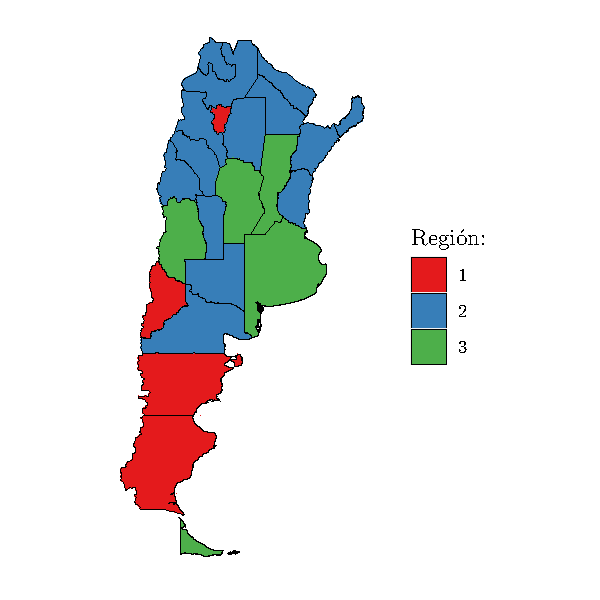
\includegraphics[scale=0.7]{./graficos/mapa_regiones.pdf}
\label{figure:mapa_reg}
\end{center}
\end{figure}

\subsection{Flujos migratorios}

Dentro de las regiones existen provincias de las cuales salen una gran cantidad de emigrantes, al igual que existen provincias que son receptoras de estos mismos, estos configuran los flujos migratorios internos del país. En primer lugar se caracterizará a las regiones según el nivel de expulsión de migrantes interprovinciales.
\begin{table}[!htbp] \centering 
\footnotesize
  \caption{\\Regiones de origen de los migrantes} 
  \label{cuadro:origen_mig} 
\begin{tabular}{@{\extracolsep{5pt}} ccc} 
\\[-1.8ex]\hline 
\hline \\[-1.8ex] 
Región & Porcentaje \\ 
\\[-1.8ex]\hline 
\hline \\[-1.8ex] 

 Sur & 16.68\%\\ 
 Norte & 49.87\%\\ 
 Centro & 33.45\%\\ 
\hline \\[-1.8ex] 
\end{tabular} 
\begin{flushleft}
\begin{scriptsize}
Fuente: Elaboración propia en base a EPH.\\
Nota: Los migrantes están definidos como personas que vivían hace cinco años en otra provincia.\\
Las estimaciones corresponden al período desde el segundo trimestre de 2016 hasta el cuarto trimestre de 2019.\\
\end{scriptsize}
\end{flushleft}
\end{table} 

En la Tabla \ref{cuadro:origen_mig} se puede notar que las provincias de la  \textbf{Región Norte} son las que mayor nivel de expulsión poseen, seguidas por las provincias pertenecientes a la Región Centro, y por úlitmo se encuentran las pertenecientes a la Región Sur.

Analizando cuales son las regiones de destino  con mayor porcentaje  de migrantes, se puede encontrar en la Tabla \ref{cuadro:destino_mig} que la \textbf{Región Centro} es la que mayor nivel de atracción posee por elevada diferencia (55.28\%), seguida por la Región Norte y en último lugar la Región Sur.

\begin{table}[!htbp] \centering 
\footnotesize
  \caption{\\Regiones de destino de los migrantes} 
  \label{cuadro:destino_mig} 
\begin{tabular}{@{\extracolsep{5pt}} ccc} 
\\[-1.8ex]\hline 
\hline \\[-1.8ex] 
Región & Porcentaje \\ 
\\[-1.8ex]\hline 
\hline \\[-1.8ex]
Sur & 14.93\%\\ 
Norte & 29.79\%\\ 
Centro & 55.28\%\\ 
\hline \\[-1.8ex] 
\end{tabular} 
\begin{flushleft}
\begin{scriptsize}
Fuente: Elaboración propia en base a EPH.\\
Nota: Los migrantes están definidos como personas que vivían hace cinco años en otra provincia.\\
Las estimaciones corresponden al período desde el segundo trimestre de 2016 hasta el cuarto trimestre de 2019.\\
\end{scriptsize}
\end{flushleft}
\end{table} 


Esta relación entre regiones con mayor atracción y expulsión de migrantes tambien puede ser vista a nivel provincial. Para ello se definen la tasa de emigración, que es el cociente entre la cantidad de emigrantes nativos de la provincia ``$x$'' sobre la cantidad de residentes de la provincia ``$x$'' y la tasa de inmigración que indica la cantidad de inmigrantes que habitan la provincia ``$x$'' sobre la cantidad de residentes de la provincia ``$x$''.

\begin{figure}[htbp!]
\begin{center}
\caption{\\Tasa de inmigración y emigración por provincia}
% Created by tikzDevice version 0.12.3.1 on 2021-05-21 22:18:04
% !TEX encoding = UTF-8 Unicode
\begin{tikzpicture}[x=1pt,y=1pt]
\definecolor{fillColor}{RGB}{255,255,255}
\path[use as bounding box,fill=fillColor,fill opacity=0.00] (0,0) rectangle (433.62,289.08);
\begin{scope}
\path[clip] (  0.00,  0.00) rectangle (433.62,289.08);
\definecolor{drawColor}{RGB}{255,255,255}
\definecolor{fillColor}{RGB}{255,255,255}

\path[draw=drawColor,line width= 0.6pt,line join=round,line cap=round,fill=fillColor] (  0.00,  0.00) rectangle (433.62,289.08);
\end{scope}
\begin{scope}
\path[clip] ( 26.79, 22.04) rectangle (364.14,266.40);
\definecolor{drawColor}{RGB}{255,255,255}

\path[draw=drawColor,line width= 0.3pt,line join=round] ( 26.79, 62.77) --
	(364.14, 62.77);

\path[draw=drawColor,line width= 0.3pt,line join=round] ( 26.79,122.01) --
	(364.14,122.01);

\path[draw=drawColor,line width= 0.3pt,line join=round] ( 26.79,181.25) --
	(364.14,181.25);

\path[draw=drawColor,line width= 0.3pt,line join=round] ( 26.79,240.49) --
	(364.14,240.49);

\path[draw=drawColor,line width= 0.3pt,line join=round] ( 83.01, 22.04) --
	( 83.01,266.40);

\path[draw=drawColor,line width= 0.3pt,line join=round] (164.79, 22.04) --
	(164.79,266.40);

\path[draw=drawColor,line width= 0.3pt,line join=round] (246.58, 22.04) --
	(246.58,266.40);

\path[draw=drawColor,line width= 0.3pt,line join=round] (328.36, 22.04) --
	(328.36,266.40);

\path[draw=drawColor,line width= 0.6pt,line join=round] ( 26.79, 33.15) --
	(364.14, 33.15);

\path[draw=drawColor,line width= 0.6pt,line join=round] ( 26.79, 92.39) --
	(364.14, 92.39);

\path[draw=drawColor,line width= 0.6pt,line join=round] ( 26.79,151.63) --
	(364.14,151.63);

\path[draw=drawColor,line width= 0.6pt,line join=round] ( 26.79,210.87) --
	(364.14,210.87);

\path[draw=drawColor,line width= 0.6pt,line join=round] ( 42.12, 22.04) --
	( 42.12,266.40);

\path[draw=drawColor,line width= 0.6pt,line join=round] (123.90, 22.04) --
	(123.90,266.40);

\path[draw=drawColor,line width= 0.6pt,line join=round] (205.69, 22.04) --
	(205.69,266.40);

\path[draw=drawColor,line width= 0.6pt,line join=round] (287.47, 22.04) --
	(287.47,266.40);
\definecolor{drawColor}{RGB}{77,175,74}
\definecolor{fillColor}{RGB}{77,175,74}

\path[draw=drawColor,line width= 0.4pt,line join=round,line cap=round,fill=fillColor] ( 82.21, 38.37) circle (  1.96);
\definecolor{drawColor}{RGB}{55,126,184}
\definecolor{fillColor}{RGB}{55,126,184}

\path[draw=drawColor,line width= 0.4pt,line join=round,line cap=round,fill=fillColor] ( 76.90,111.06) circle (  1.96);

\path[draw=drawColor,line width= 0.4pt,line join=round,line cap=round,fill=fillColor] ( 63.50,247.09) circle (  1.96);
\definecolor{drawColor}{RGB}{228,26,28}
\definecolor{fillColor}{RGB}{228,26,28}

\path[draw=drawColor,line width= 0.4pt,line join=round,line cap=round,fill=fillColor] (113.40, 61.30) circle (  1.96);
\definecolor{drawColor}{RGB}{77,175,74}
\definecolor{fillColor}{RGB}{77,175,74}

\path[draw=drawColor,line width= 0.4pt,line join=round,line cap=round,fill=fillColor] ( 80.08, 37.28) circle (  1.96);

\path[draw=drawColor,line width= 0.4pt,line join=round,line cap=round,fill=fillColor] ( 78.84, 63.57) circle (  1.96);
\definecolor{drawColor}{RGB}{55,126,184}
\definecolor{fillColor}{RGB}{55,126,184}

\path[draw=drawColor,line width= 0.4pt,line join=round,line cap=round,fill=fillColor] ( 73.72,220.69) circle (  1.96);

\path[draw=drawColor,line width= 0.4pt,line join=round,line cap=round,fill=fillColor] ( 66.53,195.39) circle (  1.96);

\path[draw=drawColor,line width= 0.4pt,line join=round,line cap=round,fill=fillColor] ( 58.75,132.92) circle (  1.96);

\path[draw=drawColor,line width= 0.4pt,line join=round,line cap=round,fill=fillColor] ( 73.94,111.78) circle (  1.96);

\path[draw=drawColor,line width= 0.4pt,line join=round,line cap=round,fill=fillColor] (104.00,111.07) circle (  1.96);

\path[draw=drawColor,line width= 0.4pt,line join=round,line cap=round,fill=fillColor] ( 93.60, 80.40) circle (  1.96);
\definecolor{drawColor}{RGB}{77,175,74}
\definecolor{fillColor}{RGB}{77,175,74}

\path[draw=drawColor,line width= 0.4pt,line join=round,line cap=round,fill=fillColor] ( 71.56, 62.83) circle (  1.96);
\definecolor{drawColor}{RGB}{55,126,184}
\definecolor{fillColor}{RGB}{55,126,184}

\path[draw=drawColor,line width= 0.4pt,line join=round,line cap=round,fill=fillColor] ( 77.61,148.97) circle (  1.96);
\definecolor{drawColor}{RGB}{228,26,28}
\definecolor{fillColor}{RGB}{228,26,28}

\path[draw=drawColor,line width= 0.4pt,line join=round,line cap=round,fill=fillColor] (124.03, 56.87) circle (  1.96);
\definecolor{drawColor}{RGB}{55,126,184}
\definecolor{fillColor}{RGB}{55,126,184}

\path[draw=drawColor,line width= 0.4pt,line join=round,line cap=round,fill=fillColor] ( 92.65,212.40) circle (  1.96);

\path[draw=drawColor,line width= 0.4pt,line join=round,line cap=round,fill=fillColor] ( 75.42, 87.58) circle (  1.96);

\path[draw=drawColor,line width= 0.4pt,line join=round,line cap=round,fill=fillColor] ( 58.18, 76.60) circle (  1.96);

\path[draw=drawColor,line width= 0.4pt,line join=round,line cap=round,fill=fillColor] (112.49, 76.36) circle (  1.96);
\definecolor{drawColor}{RGB}{228,26,28}
\definecolor{fillColor}{RGB}{228,26,28}

\path[draw=drawColor,line width= 0.4pt,line join=round,line cap=round,fill=fillColor] (143.72, 83.37) circle (  1.96);
\definecolor{drawColor}{RGB}{77,175,74}
\definecolor{fillColor}{RGB}{77,175,74}

\path[draw=drawColor,line width= 0.4pt,line join=round,line cap=round,fill=fillColor] ( 77.75, 60.23) circle (  1.96);
\definecolor{drawColor}{RGB}{55,126,184}
\definecolor{fillColor}{RGB}{55,126,184}

\path[draw=drawColor,line width= 0.4pt,line join=round,line cap=round,fill=fillColor] ( 60.79,201.99) circle (  1.96);
\definecolor{drawColor}{RGB}{77,175,74}
\definecolor{fillColor}{RGB}{77,175,74}

\path[draw=drawColor,line width= 0.4pt,line join=round,line cap=round,fill=fillColor] (204.97, 49.35) circle (  1.96);
\definecolor{drawColor}{RGB}{228,26,28}
\definecolor{fillColor}{RGB}{228,26,28}

\path[draw=drawColor,line width= 0.4pt,line join=round,line cap=round,fill=fillColor] ( 67.48, 98.80) circle (  1.96);
\definecolor{drawColor}{RGB}{0,0,0}

\path[draw=drawColor,line width= 0.6pt,line join=round] ( 26.79, 22.04) -- (364.14,266.40);
\definecolor{drawColor}{RGB}{77,175,74}

\node[text=drawColor,anchor=base,inner sep=0pt, outer sep=0pt, scale=  0.57] at ( 90.17, 42.22) {Buenos Aires};
\definecolor{drawColor}{RGB}{55,126,184}

\node[text=drawColor,anchor=base,inner sep=0pt, outer sep=0pt, scale=  0.57] at ( 89.81,103.30) {Catamarca};

\node[text=drawColor,anchor=base,inner sep=0pt, outer sep=0pt, scale=  0.57] at ( 71.59,250.96) {Chaco};
\definecolor{drawColor}{RGB}{228,26,28}

\node[text=drawColor,anchor=base,inner sep=0pt, outer sep=0pt, scale=  0.57] at (105.42, 53.52) {Chubut};
\definecolor{drawColor}{RGB}{77,175,74}

\node[text=drawColor,anchor=base,inner sep=0pt, outer sep=0pt, scale=  0.57] at ( 73.93, 29.53) {Ciudad Autónoma de Buenos Aires};

\node[text=drawColor,anchor=base,inner sep=0pt, outer sep=0pt, scale=  0.57] at ( 89.16, 67.42) {Córdoba};
\definecolor{drawColor}{RGB}{55,126,184}

\node[text=drawColor,anchor=base,inner sep=0pt, outer sep=0pt, scale=  0.57] at ( 65.65,224.55) {Corrientes};

\node[text=drawColor,anchor=base,inner sep=0pt, outer sep=0pt, scale=  0.57] at ( 74.51,187.64) {Entre Ríos};

\node[text=drawColor,anchor=base,inner sep=0pt, outer sep=0pt, scale=  0.57] at ( 64.29,135.11) {Formosa};

\node[text=drawColor,anchor=base,inner sep=0pt, outer sep=0pt, scale=  0.57] at ( 66.01,115.59) {Jujuy};

\node[text=drawColor,anchor=base,inner sep=0pt, outer sep=0pt, scale=  0.57] at (111.99,114.90) {La Pampa};

\node[text=drawColor,anchor=base,inner sep=0pt, outer sep=0pt, scale=  0.57] at (101.69, 84.31) {La Rioja};
\definecolor{drawColor}{RGB}{77,175,74}

\node[text=drawColor,anchor=base,inner sep=0pt, outer sep=0pt, scale=  0.57] at ( 61.33, 66.71) {Mendoza};
\definecolor{drawColor}{RGB}{55,126,184}

\node[text=drawColor,anchor=base,inner sep=0pt, outer sep=0pt, scale=  0.57] at ( 72.00,142.91) {Misiones};
\definecolor{drawColor}{RGB}{228,26,28}

\node[text=drawColor,anchor=base,inner sep=0pt, outer sep=0pt, scale=  0.57] at (132.05, 49.09) {Neuquén};
\definecolor{drawColor}{RGB}{55,126,184}

\node[text=drawColor,anchor=base,inner sep=0pt, outer sep=0pt, scale=  0.57] at (100.66,204.63) {Río Negro};

\node[text=drawColor,anchor=base,inner sep=0pt, outer sep=0pt, scale=  0.57] at ( 65.08, 91.01) {Salta};

\node[text=drawColor,anchor=base,inner sep=0pt, outer sep=0pt, scale=  0.57] at ( 50.13, 80.49) {San Juan};

\node[text=drawColor,anchor=base,inner sep=0pt, outer sep=0pt, scale=  0.57] at (120.56, 68.58) {San Luis};
\definecolor{drawColor}{RGB}{228,26,28}

\node[text=drawColor,anchor=base,inner sep=0pt, outer sep=0pt, scale=  0.57] at (151.77, 87.27) {Santa Cruz};
\definecolor{drawColor}{RGB}{77,175,74}

\node[text=drawColor,anchor=base,inner sep=0pt, outer sep=0pt, scale=  0.57] at ( 69.80, 52.48) {Santa Fe};
\definecolor{drawColor}{RGB}{55,126,184}

\node[text=drawColor,anchor=base,inner sep=0pt, outer sep=0pt, scale=  0.57] at ( 53.96,205.85) {Santiago del Estero};
\definecolor{drawColor}{RGB}{77,175,74}

\node[text=drawColor,anchor=base,inner sep=0pt, outer sep=0pt, scale=  0.57] at (214.31, 41.49) {Tierra del Fuego, Antártida e Islas del Atlántico Sur};
\definecolor{drawColor}{RGB}{228,26,28}

\node[text=drawColor,anchor=base,inner sep=0pt, outer sep=0pt, scale=  0.57] at ( 58.51,102.70) {Tucumán};
\end{scope}
\begin{scope}
\path[clip] (  0.00,  0.00) rectangle (433.62,289.08);
\definecolor{drawColor}{RGB}{0,0,0}

\path[draw=drawColor,line width= 0.6pt,line join=round] ( 26.79, 22.04) --
	( 26.79,266.40);
\end{scope}
\begin{scope}
\path[clip] (  0.00,  0.00) rectangle (433.62,289.08);
\definecolor{drawColor}{RGB}{0,0,0}

\node[text=drawColor,anchor=base east,inner sep=0pt, outer sep=0pt, scale=  0.50] at ( 21.84, 31.42) {0{\%}};

\node[text=drawColor,anchor=base east,inner sep=0pt, outer sep=0pt, scale=  0.50] at ( 21.84, 90.66) {20{\%}};

\node[text=drawColor,anchor=base east,inner sep=0pt, outer sep=0pt, scale=  0.50] at ( 21.84,149.90) {40{\%}};

\node[text=drawColor,anchor=base east,inner sep=0pt, outer sep=0pt, scale=  0.50] at ( 21.84,209.14) {60{\%}};
\end{scope}
\begin{scope}
\path[clip] (  0.00,  0.00) rectangle (433.62,289.08);
\definecolor{drawColor}{gray}{0.20}

\path[draw=drawColor,line width= 0.6pt,line join=round] ( 24.04, 33.15) --
	( 26.79, 33.15);

\path[draw=drawColor,line width= 0.6pt,line join=round] ( 24.04, 92.39) --
	( 26.79, 92.39);

\path[draw=drawColor,line width= 0.6pt,line join=round] ( 24.04,151.63) --
	( 26.79,151.63);

\path[draw=drawColor,line width= 0.6pt,line join=round] ( 24.04,210.87) --
	( 26.79,210.87);
\end{scope}
\begin{scope}
\path[clip] (  0.00,  0.00) rectangle (433.62,289.08);
\definecolor{drawColor}{RGB}{0,0,0}

\path[draw=drawColor,line width= 0.6pt,line join=round] ( 26.79, 22.04) --
	(364.14, 22.04);
\end{scope}
\begin{scope}
\path[clip] (  0.00,  0.00) rectangle (433.62,289.08);
\definecolor{drawColor}{gray}{0.20}

\path[draw=drawColor,line width= 0.6pt,line join=round] ( 42.12, 19.29) --
	( 42.12, 22.04);

\path[draw=drawColor,line width= 0.6pt,line join=round] (123.90, 19.29) --
	(123.90, 22.04);

\path[draw=drawColor,line width= 0.6pt,line join=round] (205.69, 19.29) --
	(205.69, 22.04);

\path[draw=drawColor,line width= 0.6pt,line join=round] (287.47, 19.29) --
	(287.47, 22.04);
\end{scope}
\begin{scope}
\path[clip] (  0.00,  0.00) rectangle (433.62,289.08);
\definecolor{drawColor}{RGB}{0,0,0}

\node[text=drawColor,anchor=base,inner sep=0pt, outer sep=0pt, scale=  0.50] at ( 42.12, 13.64) {0{\%}};

\node[text=drawColor,anchor=base,inner sep=0pt, outer sep=0pt, scale=  0.50] at (123.90, 13.64) {20{\%}};

\node[text=drawColor,anchor=base,inner sep=0pt, outer sep=0pt, scale=  0.50] at (205.69, 13.64) {40{\%}};

\node[text=drawColor,anchor=base,inner sep=0pt, outer sep=0pt, scale=  0.50] at (287.47, 13.64) {60{\%}};
\end{scope}
\begin{scope}
\path[clip] (  0.00,  0.00) rectangle (433.62,289.08);
\definecolor{drawColor}{RGB}{0,0,0}

\node[text=drawColor,anchor=base,inner sep=0pt, outer sep=0pt, scale=  0.50] at (195.46,  6.47) {\bfseries Tasa de inmigración};
\end{scope}
\begin{scope}
\path[clip] (  0.00,  0.00) rectangle (433.62,289.08);
\definecolor{drawColor}{RGB}{0,0,0}

\node[text=drawColor,rotate= 90.00,anchor=base,inner sep=0pt, outer sep=0pt, scale=  0.50] at (  8.95,144.22) {\bfseries Tasa de emigración};
\end{scope}
\begin{scope}
\path[clip] (  0.00,  0.00) rectangle (433.62,289.08);
\definecolor{fillColor}{RGB}{255,255,255}

\path[fill=fillColor] (375.14,109.43) rectangle (428.12,179.02);
\end{scope}
\begin{scope}
\path[clip] (  0.00,  0.00) rectangle (433.62,289.08);
\definecolor{drawColor}{RGB}{0,0,0}

\node[text=drawColor,anchor=base west,inner sep=0pt, outer sep=0pt, scale=  1.10] at (380.64,164.86) {\bfseries Región:};
\end{scope}
\begin{scope}
\path[clip] (  0.00,  0.00) rectangle (433.62,289.08);
\definecolor{drawColor}{RGB}{228,26,28}
\definecolor{fillColor}{RGB}{228,26,28}

\path[draw=drawColor,line width= 0.4pt,line join=round,line cap=round,fill=fillColor] (387.87,151.06) circle (  1.96);
\end{scope}
\begin{scope}
\path[clip] (  0.00,  0.00) rectangle (433.62,289.08);
\definecolor{drawColor}{RGB}{55,126,184}
\definecolor{fillColor}{RGB}{55,126,184}

\path[draw=drawColor,line width= 0.4pt,line join=round,line cap=round,fill=fillColor] (387.87,136.61) circle (  1.96);
\end{scope}
\begin{scope}
\path[clip] (  0.00,  0.00) rectangle (433.62,289.08);
\definecolor{drawColor}{RGB}{77,175,74}
\definecolor{fillColor}{RGB}{77,175,74}

\path[draw=drawColor,line width= 0.4pt,line join=round,line cap=round,fill=fillColor] (387.87,122.15) circle (  1.96);
\end{scope}
\begin{scope}
\path[clip] (  0.00,  0.00) rectangle (433.62,289.08);
\definecolor{drawColor}{RGB}{0,0,0}

\node[text=drawColor,anchor=base west,inner sep=0pt, outer sep=0pt, scale=  0.88] at (400.59,148.03) {1};
\end{scope}
\begin{scope}
\path[clip] (  0.00,  0.00) rectangle (433.62,289.08);
\definecolor{drawColor}{RGB}{0,0,0}

\node[text=drawColor,anchor=base west,inner sep=0pt, outer sep=0pt, scale=  0.88] at (400.59,133.58) {2};
\end{scope}
\begin{scope}
\path[clip] (  0.00,  0.00) rectangle (433.62,289.08);
\definecolor{drawColor}{RGB}{0,0,0}

\node[text=drawColor,anchor=base west,inner sep=0pt, outer sep=0pt, scale=  0.88] at (400.59,119.12) {3};
\end{scope}
\end{tikzpicture}

\label{figure:emig_inmig_prov}
\end{center}
\begin{flushleft}
\begin{scriptsize}
Fuente: Elaboración propia en base a EPH.\\
Nota: Los migrantes están definidos como personas que vivían hace cinco años en otra provincia.\\
Las estimaciones corresponden al período desde el segundo trimestre de 2016 hasta el cuarto trimestre de 2019.\\
\end{scriptsize}
\end{flushleft}
\end{figure}

En la Figura \ref{figure:emig_inmig_prov} se puede observar la relación entre la tasa de emigración e inmigración de las provincias, diferenciadas por la región a la cual pertenecen.

La bisectriz divide el plano en dos zonas, todas las provincias que se encuentran por encima de ella son aquellas en la que la tasa de emigración es superior a la tasa de inmigración, mientras que las que se encuentran por debajo son quellas en la que existe una mayor tasa de inmigración que de emigración. 

Las provincias pertenecientes a la Región Norte se ubican en casi su totalidad por encima de la bisectriz, indicando que son provincias en donde la expulsión de migrantes es mucho mayor que la atracción de los mismos. Las provincias de la Región Sur tienen una mayor tendencia a ubicarse por encima de la linea diagonal, con excepción de Neuquén y Tierra del Fuego. Por último, en la Región Centro todas las provincias se encuentran por debajo de la diagonal, en donde la atracción de migrantes es mayor que su nivel de expulsión.

Estas diferencias entre tasa de emigración e inmigración pueden ser vistas desde un punto de vista geográfico en la Figura \ref{figure:emig_inmig_prov_mapa}. Se observa la diferencia en la distribución de las provincias con mayor tasa de migración e inmigración, las provincias de Rio Negro, Santa Cruz y La Pampa son las que mayores tasa de emigración poseen, mientras que Tierra del Fuego, Santa Cruz y Neuquén son  las provincias en donde la tasa de inmigración es más elevada.
\begin{figure}[htbp!]
\begin{center}
\caption{\\Mapa de tasas de emigración e inmigración por provincia}
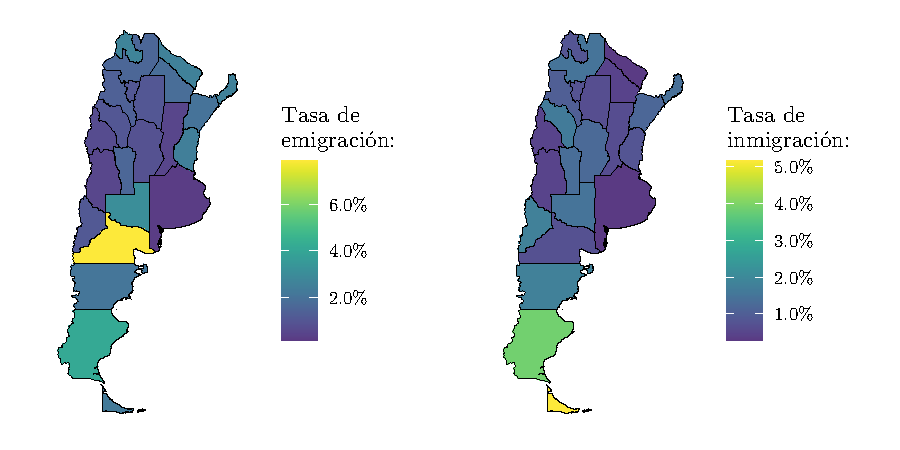
\includegraphics[scale=1.1]{./graficos/emig_inmig_por_prov.pdf}
\label{figure:emig_inmig_prov_mapa}
\end{center}
\begin{flushleft}
\begin{scriptsize}
Fuente: Elaboración propia en base a EPH.\\
Nota: Los migrantes están definidos como personas que vivían hace cinco años en otra provincia.\\
Las estimaciones corresponden al período desde el segundo trimestre de 2016 hasta el cuarto trimestre de 2019.\\
\end{scriptsize}
\end{flushleft}
\end{figure}
\newpage
\section{Migrantes}
Un migrante es toda persona que se traslada fuera de su localidad de residencia habitual de manera temporal o permanente. En este trabajo solamente se tienen en cuenta los casos en los que este movimiento migratorio se realiza dentro del mismo país, y considerando que el mismo haya sido emprendido hace cinco años o menos. El último punto es importante para que las características que se tomen como determinantes de la migración tengan un correlato con la decisión migratoria. Un nativo, como figura contrapuesta al migrante, será la persona que haya nacido y este viviendo en la misma provincia en los últimos cinco años desde el relevamiento.

Las características individuales o familiares de las personas que toman la decisión de emprender un proceso migratorio forman parte de los microdeterminantes de las migraciones. Si bien estos no deben ser tomados como los principales impulsores de la decisión del éxodo, funcionan como mediadores en la decisión migratoria y tienen una elevada influencia en la auto-selección de los migrantes para cada una de las regiones.

En las siguientes subsecciones se analizará si existen características que provoquen que ciertas personas posean una mayor propensión a migrar hacia determinadas localizaciones. Para ello se indagará en las diferencias entre los migrantes y los nativos de las distintas regiones con respecto a los microdeterminantes que se consideran relevantes, los cuales serán explicitados y desarrollados en los siguientes apartados.


\subsection{Género y edad}
El género y la edad de las personas son considerados dentro de los microfactores que pueden afectar considerablemente a la decisión migratoria, es por ello que se analizan estas características para los nativos y migrantes de cada región.

En las últimas decadas la dimensión del género en la migración ha tomado un sendero particular, en gran parte por la participación más activa de la mujer en el mercado laboral y el acceso a la posibilidad de una mayor independencia económica. Todo esto provocó que la mujer tome un rol más activo en la decisión migratoria individual, permitiendole desligarse de la decisión migratoria respondiendo a estrategias  familiares.


En la Figura \ref{figure:sexo_mig_} se puede ver el género de los migrantes y nativos. En las tres regiones los migrantes son en su mayoría mujeres, siendo la Región Sur la que mayor cantidad de migrantes mujeres posee con un $51.07\%$, mientras que la Región Norte es la que menor proporción de migrantes mujeres posee, con un $50.47\%$ de migrantes mujeres.

La edad de las personas no solo afecta el horizonte temporal en el que toman las decisiones, sino que también condiciona el nivel de aversión al riesgo, escalas de incentivos e inclusive determina preferencias y hábitos.

\begin{figure}[ht!]
\begin{center}
 	\caption{\\Sexo de los nativos y migrantes por regiones}
% Created by tikzDevice version 0.12.3.1 on 2021-05-22 21:10:22
% !TEX encoding = UTF-8 Unicode
\begin{tikzpicture}[x=1pt,y=1pt]
\definecolor{fillColor}{RGB}{255,255,255}
\path[use as bounding box,fill=fillColor,fill opacity=0.00] (0,0) rectangle (433.62,289.08);
\begin{scope}
\path[clip] (  0.00,  0.00) rectangle (433.62,289.08);
\definecolor{drawColor}{RGB}{255,255,255}
\definecolor{fillColor}{RGB}{255,255,255}

\path[draw=drawColor,line width= 0.6pt,line join=round,line cap=round,fill=fillColor] (  0.00,  0.00) rectangle (433.62,289.08);
\end{scope}
\begin{scope}
\path[clip] ( 61.11,202.95) rectangle (335.80,283.58);
\definecolor{drawColor}{RGB}{255,255,255}

\path[draw=drawColor,line width= 0.3pt,line join=round] (104.81,202.95) --
	(104.81,283.58);

\path[draw=drawColor,line width= 0.3pt,line join=round] (167.24,202.95) --
	(167.24,283.58);

\path[draw=drawColor,line width= 0.3pt,line join=round] (229.67,202.95) --
	(229.67,283.58);

\path[draw=drawColor,line width= 0.3pt,line join=round] (292.10,202.95) --
	(292.10,283.58);

\path[draw=drawColor,line width= 0.6pt,line join=round] ( 61.11,224.94) --
	(335.80,224.94);

\path[draw=drawColor,line width= 0.6pt,line join=round] ( 61.11,261.59) --
	(335.80,261.59);

\path[draw=drawColor,line width= 0.6pt,line join=round] ( 73.60,202.95) --
	( 73.60,283.58);

\path[draw=drawColor,line width= 0.6pt,line join=round] (136.03,202.95) --
	(136.03,283.58);

\path[draw=drawColor,line width= 0.6pt,line join=round] (198.45,202.95) --
	(198.45,283.58);

\path[draw=drawColor,line width= 0.6pt,line join=round] (260.88,202.95) --
	(260.88,283.58);

\path[draw=drawColor,line width= 0.6pt,line join=round] (323.31,202.95) --
	(323.31,283.58);
\definecolor{fillColor}{RGB}{228,26,28}

\path[fill=fillColor] (205.44,213.94) rectangle (323.31,235.93);
\definecolor{fillColor}{RGB}{55,126,184}

\path[fill=fillColor] ( 73.60,213.94) rectangle (205.44,235.93);
\definecolor{fillColor}{RGB}{228,26,28}

\path[fill=fillColor] (202.38,250.59) rectangle (323.31,272.58);
\definecolor{fillColor}{RGB}{55,126,184}

\path[fill=fillColor] ( 73.60,250.59) rectangle (202.38,272.58);
\definecolor{drawColor}{RGB}{0,0,0}

\node[text=drawColor,anchor=base,inner sep=0pt, outer sep=0pt, scale=  0.85] at (252.59,222.00) {47.20{\%}};

\node[text=drawColor,anchor=base,inner sep=0pt, outer sep=0pt, scale=  0.85] at (126.33,222.00) {52.80{\%}};

\node[text=drawColor,anchor=base,inner sep=0pt, outer sep=0pt, scale=  0.85] at (250.75,258.65) {48.43{\%}};

\node[text=drawColor,anchor=base,inner sep=0pt, outer sep=0pt, scale=  0.85] at (125.11,258.65) {51.57{\%}};
\end{scope}
\begin{scope}
\path[clip] ( 61.11,116.82) rectangle (335.80,197.45);
\definecolor{drawColor}{RGB}{255,255,255}

\path[draw=drawColor,line width= 0.3pt,line join=round] (104.81,116.82) --
	(104.81,197.45);

\path[draw=drawColor,line width= 0.3pt,line join=round] (167.24,116.82) --
	(167.24,197.45);

\path[draw=drawColor,line width= 0.3pt,line join=round] (229.67,116.82) --
	(229.67,197.45);

\path[draw=drawColor,line width= 0.3pt,line join=round] (292.10,116.82) --
	(292.10,197.45);

\path[draw=drawColor,line width= 0.6pt,line join=round] ( 61.11,138.81) --
	(335.80,138.81);

\path[draw=drawColor,line width= 0.6pt,line join=round] ( 61.11,175.46) --
	(335.80,175.46);

\path[draw=drawColor,line width= 0.6pt,line join=round] ( 73.60,116.82) --
	( 73.60,197.45);

\path[draw=drawColor,line width= 0.6pt,line join=round] (136.03,116.82) --
	(136.03,197.45);

\path[draw=drawColor,line width= 0.6pt,line join=round] (198.45,116.82) --
	(198.45,197.45);

\path[draw=drawColor,line width= 0.6pt,line join=round] (260.88,116.82) --
	(260.88,197.45);

\path[draw=drawColor,line width= 0.6pt,line join=round] (323.31,116.82) --
	(323.31,197.45);
\definecolor{fillColor}{RGB}{228,26,28}

\path[fill=fillColor] (207.27,127.81) rectangle (323.31,149.80);
\definecolor{fillColor}{RGB}{55,126,184}

\path[fill=fillColor] ( 73.60,127.81) rectangle (207.27,149.80);
\definecolor{fillColor}{RGB}{228,26,28}

\path[fill=fillColor] (203.16,164.46) rectangle (323.31,186.45);
\definecolor{fillColor}{RGB}{55,126,184}

\path[fill=fillColor] ( 73.60,164.46) rectangle (203.16,186.45);
\definecolor{drawColor}{RGB}{0,0,0}

\node[text=drawColor,anchor=base,inner sep=0pt, outer sep=0pt, scale=  0.85] at (253.68,135.87) {46.47{\%}};

\node[text=drawColor,anchor=base,inner sep=0pt, outer sep=0pt, scale=  0.85] at (127.07,135.87) {53.53{\%}};

\node[text=drawColor,anchor=base,inner sep=0pt, outer sep=0pt, scale=  0.85] at (251.22,172.52) {48.11{\%}};

\node[text=drawColor,anchor=base,inner sep=0pt, outer sep=0pt, scale=  0.85] at (125.42,172.52) {51.89{\%}};
\end{scope}
\begin{scope}
\path[clip] ( 61.11, 30.69) rectangle (335.80,111.32);
\definecolor{drawColor}{RGB}{255,255,255}

\path[draw=drawColor,line width= 0.3pt,line join=round] (104.81, 30.69) --
	(104.81,111.32);

\path[draw=drawColor,line width= 0.3pt,line join=round] (167.24, 30.69) --
	(167.24,111.32);

\path[draw=drawColor,line width= 0.3pt,line join=round] (229.67, 30.69) --
	(229.67,111.32);

\path[draw=drawColor,line width= 0.3pt,line join=round] (292.10, 30.69) --
	(292.10,111.32);

\path[draw=drawColor,line width= 0.6pt,line join=round] ( 61.11, 52.68) --
	(335.80, 52.68);

\path[draw=drawColor,line width= 0.6pt,line join=round] ( 61.11, 89.33) --
	(335.80, 89.33);

\path[draw=drawColor,line width= 0.6pt,line join=round] ( 73.60, 30.69) --
	( 73.60,111.32);

\path[draw=drawColor,line width= 0.6pt,line join=round] (136.03, 30.69) --
	(136.03,111.32);

\path[draw=drawColor,line width= 0.6pt,line join=round] (198.45, 30.69) --
	(198.45,111.32);

\path[draw=drawColor,line width= 0.6pt,line join=round] (260.88, 30.69) --
	(260.88,111.32);

\path[draw=drawColor,line width= 0.6pt,line join=round] (323.31, 30.69) --
	(323.31,111.32);
\definecolor{fillColor}{RGB}{228,26,28}

\path[fill=fillColor] (212.48, 41.68) rectangle (323.31, 63.67);
\definecolor{fillColor}{RGB}{55,126,184}

\path[fill=fillColor] ( 73.60, 41.68) rectangle (212.48, 63.67);
\definecolor{fillColor}{RGB}{228,26,28}

\path[fill=fillColor] (201.44, 78.33) rectangle (323.31,100.32);
\definecolor{fillColor}{RGB}{55,126,184}

\path[fill=fillColor] ( 73.60, 78.33) rectangle (201.44,100.32);
\definecolor{drawColor}{RGB}{0,0,0}

\node[text=drawColor,anchor=base,inner sep=0pt, outer sep=0pt, scale=  0.85] at (256.81, 49.74) {44.38{\%}};

\node[text=drawColor,anchor=base,inner sep=0pt, outer sep=0pt, scale=  0.85] at (129.15, 49.74) {55.62{\%}};

\node[text=drawColor,anchor=base,inner sep=0pt, outer sep=0pt, scale=  0.85] at (250.19, 86.39) {48.80{\%}};

\node[text=drawColor,anchor=base,inner sep=0pt, outer sep=0pt, scale=  0.85] at (124.74, 86.39) {51.20{\%}};
\end{scope}
\begin{scope}
\path[clip] (335.80,202.95) rectangle (352.37,283.58);
\definecolor{drawColor}{gray}{0.10}

\node[text=drawColor,rotate=-90.00,anchor=base,inner sep=0pt, outer sep=0pt, scale=  0.88] at (341.05,243.26) {\textbf{\{}Región1{\}}};
\end{scope}
\begin{scope}
\path[clip] (335.80,116.82) rectangle (352.37,197.45);
\definecolor{drawColor}{gray}{0.10}

\node[text=drawColor,rotate=-90.00,anchor=base,inner sep=0pt, outer sep=0pt, scale=  0.88] at (341.05,157.13) {\textbf{\{}Región2{\}}};
\end{scope}
\begin{scope}
\path[clip] (335.80, 30.69) rectangle (352.37,111.32);
\definecolor{drawColor}{gray}{0.10}

\node[text=drawColor,rotate=-90.00,anchor=base,inner sep=0pt, outer sep=0pt, scale=  0.88] at (341.05, 71.00) {\textbf{\{}Región3{\}}};
\end{scope}
\begin{scope}
\path[clip] (  0.00,  0.00) rectangle (433.62,289.08);
\definecolor{drawColor}{gray}{0.20}

\path[draw=drawColor,line width= 0.6pt,line join=round] ( 73.60, 27.94) --
	( 73.60, 30.69);

\path[draw=drawColor,line width= 0.6pt,line join=round] (136.03, 27.94) --
	(136.03, 30.69);

\path[draw=drawColor,line width= 0.6pt,line join=round] (198.45, 27.94) --
	(198.45, 30.69);

\path[draw=drawColor,line width= 0.6pt,line join=round] (260.88, 27.94) --
	(260.88, 30.69);

\path[draw=drawColor,line width= 0.6pt,line join=round] (323.31, 27.94) --
	(323.31, 30.69);
\end{scope}
\begin{scope}
\path[clip] (  0.00,  0.00) rectangle (433.62,289.08);
\definecolor{drawColor}{RGB}{0,0,0}

\node[text=drawColor,anchor=base,inner sep=0pt, outer sep=0pt, scale=  0.88] at ( 73.60, 19.68) {0{\%}};

\node[text=drawColor,anchor=base,inner sep=0pt, outer sep=0pt, scale=  0.88] at (136.03, 19.68) {25{\%}};

\node[text=drawColor,anchor=base,inner sep=0pt, outer sep=0pt, scale=  0.88] at (198.45, 19.68) {50{\%}};

\node[text=drawColor,anchor=base,inner sep=0pt, outer sep=0pt, scale=  0.88] at (260.88, 19.68) {75{\%}};

\node[text=drawColor,anchor=base,inner sep=0pt, outer sep=0pt, scale=  0.88] at (323.31, 19.68) {100{\%}};
\end{scope}
\begin{scope}
\path[clip] (  0.00,  0.00) rectangle (433.62,289.08);
\definecolor{drawColor}{RGB}{0,0,0}

\node[text=drawColor,anchor=base east,inner sep=0pt, outer sep=0pt, scale=  0.88] at ( 56.16,221.91) {Migrantes};

\node[text=drawColor,anchor=base east,inner sep=0pt, outer sep=0pt, scale=  0.88] at ( 56.16,258.56) {Nativos};
\end{scope}
\begin{scope}
\path[clip] (  0.00,  0.00) rectangle (433.62,289.08);
\definecolor{drawColor}{gray}{0.20}

\path[draw=drawColor,line width= 0.6pt,line join=round] ( 58.36,224.94) --
	( 61.11,224.94);

\path[draw=drawColor,line width= 0.6pt,line join=round] ( 58.36,261.59) --
	( 61.11,261.59);
\end{scope}
\begin{scope}
\path[clip] (  0.00,  0.00) rectangle (433.62,289.08);
\definecolor{drawColor}{RGB}{0,0,0}

\node[text=drawColor,anchor=base east,inner sep=0pt, outer sep=0pt, scale=  0.88] at ( 56.16,135.78) {Migrantes};

\node[text=drawColor,anchor=base east,inner sep=0pt, outer sep=0pt, scale=  0.88] at ( 56.16,172.43) {Nativos};
\end{scope}
\begin{scope}
\path[clip] (  0.00,  0.00) rectangle (433.62,289.08);
\definecolor{drawColor}{gray}{0.20}

\path[draw=drawColor,line width= 0.6pt,line join=round] ( 58.36,138.81) --
	( 61.11,138.81);

\path[draw=drawColor,line width= 0.6pt,line join=round] ( 58.36,175.46) --
	( 61.11,175.46);
\end{scope}
\begin{scope}
\path[clip] (  0.00,  0.00) rectangle (433.62,289.08);
\definecolor{drawColor}{RGB}{0,0,0}

\node[text=drawColor,anchor=base east,inner sep=0pt, outer sep=0pt, scale=  0.88] at ( 56.16, 49.65) {Migrantes};

\node[text=drawColor,anchor=base east,inner sep=0pt, outer sep=0pt, scale=  0.88] at ( 56.16, 86.30) {Nativos};
\end{scope}
\begin{scope}
\path[clip] (  0.00,  0.00) rectangle (433.62,289.08);
\definecolor{drawColor}{gray}{0.20}

\path[draw=drawColor,line width= 0.6pt,line join=round] ( 58.36, 52.68) --
	( 61.11, 52.68);

\path[draw=drawColor,line width= 0.6pt,line join=round] ( 58.36, 89.33) --
	( 61.11, 89.33);
\end{scope}
\begin{scope}
\path[clip] (  0.00,  0.00) rectangle (433.62,289.08);
\definecolor{fillColor}{RGB}{255,255,255}

\path[fill=fillColor] (363.37,129.57) rectangle (428.12,184.69);
\end{scope}
\begin{scope}
\path[clip] (  0.00,  0.00) rectangle (433.62,289.08);
\definecolor{fillColor}{gray}{0.95}

\path[fill=fillColor] (368.87,149.53) rectangle (383.32,163.98);
\end{scope}
\begin{scope}
\path[clip] (  0.00,  0.00) rectangle (433.62,289.08);
\definecolor{fillColor}{RGB}{228,26,28}

\path[fill=fillColor] (369.58,150.24) rectangle (382.61,163.27);
\end{scope}
\begin{scope}
\path[clip] (  0.00,  0.00) rectangle (433.62,289.08);
\definecolor{fillColor}{gray}{0.95}

\path[fill=fillColor] (368.87,135.07) rectangle (383.32,149.53);
\end{scope}
\begin{scope}
\path[clip] (  0.00,  0.00) rectangle (433.62,289.08);
\definecolor{fillColor}{RGB}{55,126,184}

\path[fill=fillColor] (369.58,135.78) rectangle (382.61,148.81);
\end{scope}
\begin{scope}
\path[clip] (  0.00,  0.00) rectangle (433.62,289.08);
\definecolor{drawColor}{RGB}{0,0,0}

\node[text=drawColor,anchor=base west,inner sep=0pt, outer sep=0pt, scale=  0.88] at (388.82,153.72) {Hombres};
\end{scope}
\begin{scope}
\path[clip] (  0.00,  0.00) rectangle (433.62,289.08);
\definecolor{drawColor}{RGB}{0,0,0}

\node[text=drawColor,anchor=base west,inner sep=0pt, outer sep=0pt, scale=  0.88] at (388.82,139.27) {Mujeres};
\end{scope}
\end{tikzpicture}
 
 	\label{figure:sexo_mig_}
\begin{flushleft}
\begin{scriptsize}
Fuente: Elaboración propia en base a EPH.\\
Nota: Los migrantes están definidos como personas que vivían hace cinco años en otra provincia. Los nativos están definidos como personas que nacieron y viven en la misma provincia. Las estimaciones corresponden al período desde el segundo trimestre de 2016 hasta el cuarto trimestre de 2019.\\
\end{scriptsize}
\end{flushleft}
\end{center}
\end{figure}
\newpage


En la Figura \ref{figure:edad_mig} se puede observar la función de densidad de la edad de los nativos y migrantes para cada una de las tres regiones. La densidad de la edad de los migrantes presenta una mayor acumulación en valores de edad considerablemente menores que la de los nativos, y esta relación se cumple para las tres regiones. En la Región Centro es en donde esta característica es más notoria, aquí la población migrante presenta un perfil etario considerablemente más juvenil en comparación con las cualidades etarias de la población nativa, la cual deja entrever una población más avejentada en término relativos.

La mayoría de los migrantes se encuentran dentro del rango etario de la Población Económicamente Activa. Las personas que se encuentran dentro de la edad laboral tienen una mayor probabilidad de sortear los obstáculos de conseguir un trabajo una vez que deciden migrar, lo que reduce sustancialmente los costos del éxodo migratorio.


\begin{figure}[ht!]
\begin{center}
\caption{\\Edad de los nativos y migrantes por regiones}
% Created by tikzDevice version 0.12.3.1 on 2021-07-01 11:54:32
% !TEX encoding = UTF-8 Unicode
\begin{tikzpicture}[x=1pt,y=1pt]
\definecolor{fillColor}{RGB}{255,255,255}
\path[use as bounding box,fill=fillColor,fill opacity=0.00] (0,0) rectangle (433.62,289.08);
\begin{scope}
\path[clip] (  0.00,  0.00) rectangle (433.62,289.08);
\definecolor{drawColor}{RGB}{255,255,255}
\definecolor{fillColor}{RGB}{255,255,255}

\path[draw=drawColor,line width= 0.6pt,line join=round,line cap=round,fill=fillColor] (  0.00, -0.00) rectangle (433.62,289.08);
\end{scope}
\begin{scope}
\path[clip] ( 41.49, 67.14) rectangle (166.70,267.01);
\definecolor{drawColor}{RGB}{255,255,255}

\path[draw=drawColor,line width= 0.3pt,line join=round] ( 41.49,104.00) --
	(166.70,104.00);

\path[draw=drawColor,line width= 0.3pt,line join=round] ( 41.49,159.56) --
	(166.70,159.56);

\path[draw=drawColor,line width= 0.3pt,line join=round] ( 41.49,215.11) --
	(166.70,215.11);

\path[draw=drawColor,line width= 0.3pt,line join=round] ( 52.87, 67.14) --
	( 52.87,267.01);

\path[draw=drawColor,line width= 0.3pt,line join=round] ( 87.02, 67.14) --
	( 87.02,267.01);

\path[draw=drawColor,line width= 0.3pt,line join=round] (121.17, 67.14) --
	(121.17,267.01);

\path[draw=drawColor,line width= 0.3pt,line join=round] (155.32, 67.14) --
	(155.32,267.01);

\path[draw=drawColor,line width= 0.6pt,line join=round] ( 41.49, 76.22) --
	(166.70, 76.22);

\path[draw=drawColor,line width= 0.6pt,line join=round] ( 41.49,131.78) --
	(166.70,131.78);

\path[draw=drawColor,line width= 0.6pt,line join=round] ( 41.49,187.33) --
	(166.70,187.33);

\path[draw=drawColor,line width= 0.6pt,line join=round] ( 41.49,242.89) --
	(166.70,242.89);

\path[draw=drawColor,line width= 0.6pt,line join=round] ( 69.94, 67.14) --
	( 69.94,267.01);

\path[draw=drawColor,line width= 0.6pt,line join=round] (104.09, 67.14) --
	(104.09,267.01);

\path[draw=drawColor,line width= 0.6pt,line join=round] (138.24, 67.14) --
	(138.24,267.01);
\definecolor{fillColor}{RGB}{228,26,28}

\path[fill=fillColor,fill opacity=0.50] ( 47.18, 76.25) --
	( 47.40, 76.26) --
	( 47.62, 76.28) --
	( 47.85, 76.30) --
	( 48.07, 76.33) --
	( 48.29, 76.37) --
	( 48.52, 76.42) --
	( 48.74, 76.49) --
	( 48.96, 76.58) --
	( 49.18, 76.69) --
	( 49.41, 76.84) --
	( 49.63, 77.04) --
	( 49.85, 77.29) --
	( 50.07, 77.60) --
	( 50.30, 77.99) --
	( 50.52, 78.46) --
	( 50.74, 79.04) --
	( 50.97, 79.76) --
	( 51.19, 80.64) --
	( 51.41, 81.69) --
	( 51.63, 82.93) --
	( 51.86, 84.39) --
	( 52.08, 86.09) --
	( 52.30, 88.06) --
	( 52.53, 90.38) --
	( 52.75, 93.03) --
	( 52.97, 96.03) --
	( 53.19, 99.38) --
	( 53.42,103.12) --
	( 53.64,107.25) --
	( 53.86,111.79) --
	( 54.08,116.80) --
	( 54.31,122.20) --
	( 54.53,127.99) --
	( 54.75,134.13) --
	( 54.98,140.62) --
	( 55.20,147.40) --
	( 55.42,154.47) --
	( 55.64,161.77) --
	( 55.87,169.21) --
	( 56.09,176.74) --
	( 56.31,184.30) --
	( 56.53,191.82) --
	( 56.76,199.25) --
	( 56.98,206.48) --
	( 57.20,213.43) --
	( 57.43,220.07) --
	( 57.65,226.32) --
	( 57.87,232.13) --
	( 58.09,237.46) --
	( 58.32,242.27) --
	( 58.54,246.43) --
	( 58.76,249.93) --
	( 58.99,252.81) --
	( 59.21,255.05) --
	( 59.43,256.64) --
	( 59.65,257.60) --
	( 59.88,257.92) --
	( 60.10,257.54) --
	( 60.32,256.56) --
	( 60.54,255.05) --
	( 60.77,253.04) --
	( 60.99,250.58) --
	( 61.21,247.71) --
	( 61.44,244.49) --
	( 61.66,240.91) --
	( 61.88,237.12) --
	( 62.10,233.15) --
	( 62.33,229.07) --
	( 62.55,224.92) --
	( 62.77,220.74) --
	( 62.99,216.58) --
	( 63.22,212.51) --
	( 63.44,208.54) --
	( 63.66,204.70) --
	( 63.89,201.02) --
	( 64.11,197.50) --
	( 64.33,194.16) --
	( 64.55,191.03) --
	( 64.78,188.10) --
	( 65.00,185.36) --
	( 65.22,182.79) --
	( 65.44,180.38) --
	( 65.67,178.11) --
	( 65.89,175.99) --
	( 66.11,173.99) --
	( 66.34,172.09) --
	( 66.56,170.27) --
	( 66.78,168.52) --
	( 67.00,166.81) --
	( 67.23,165.14) --
	( 67.45,163.49) --
	( 67.67,161.87) --
	( 67.90,160.25) --
	( 68.12,158.63) --
	( 68.34,157.02) --
	( 68.56,155.42) --
	( 68.79,153.82) --
	( 69.01,152.22) --
	( 69.23,150.65) --
	( 69.45,149.10) --
	( 69.68,147.58) --
	( 69.90,146.09) --
	( 70.12,144.65) --
	( 70.35,143.26) --
	( 70.57,141.92) --
	( 70.79,140.65) --
	( 71.01,139.44) --
	( 71.24,138.31) --
	( 71.46,137.24) --
	( 71.68,136.25) --
	( 71.90,135.32) --
	( 72.13,134.47) --
	( 72.35,133.69) --
	( 72.57,132.97) --
	( 72.80,132.31) --
	( 73.02,131.70) --
	( 73.24,131.14) --
	( 73.46,130.62) --
	( 73.69,130.13) --
	( 73.91,129.66) --
	( 74.13,129.21) --
	( 74.36,128.77) --
	( 74.58,128.33) --
	( 74.80,127.88) --
	( 75.02,127.42) --
	( 75.25,126.93) --
	( 75.47,126.42) --
	( 75.69,125.88) --
	( 75.91,125.31) --
	( 76.14,124.69) --
	( 76.36,124.05) --
	( 76.58,123.36) --
	( 76.81,122.63) --
	( 77.03,121.86) --
	( 77.25,121.07) --
	( 77.47,120.24) --
	( 77.70,119.39) --
	( 77.92,118.52) --
	( 78.14,117.63) --
	( 78.36,116.74) --
	( 78.59,115.85) --
	( 78.81,114.96) --
	( 79.03,114.08) --
	( 79.26,113.22) --
	( 79.48,112.39) --
	( 79.70,111.58) --
	( 79.92,110.81) --
	( 80.15,110.07) --
	( 80.37,109.38) --
	( 80.59,108.72) --
	( 80.82,108.10) --
	( 81.04,107.53) --
	( 81.26,107.00) --
	( 81.48,106.51) --
	( 81.71,106.06) --
	( 81.93,105.65) --
	( 82.15,105.27) --
	( 82.37,104.92) --
	( 82.60,104.60) --
	( 82.82,104.30) --
	( 83.04,104.02) --
	( 83.27,103.77) --
	( 83.49,103.52) --
	( 83.71,103.29) --
	( 83.93,103.06) --
	( 84.16,102.84) --
	( 84.38,102.62) --
	( 84.60,102.40) --
	( 84.82,102.17) --
	( 85.05,101.94) --
	( 85.27,101.71) --
	( 85.49,101.47) --
	( 85.72,101.21) --
	( 85.94,100.95) --
	( 86.16,100.68) --
	( 86.38,100.39) --
	( 86.61,100.09) --
	( 86.83, 99.78) --
	( 87.05, 99.46) --
	( 87.28, 99.13) --
	( 87.50, 98.78) --
	( 87.72, 98.43) --
	( 87.94, 98.07) --
	( 88.17, 97.70) --
	( 88.39, 97.32) --
	( 88.61, 96.95) --
	( 88.83, 96.57) --
	( 89.06, 96.19) --
	( 89.28, 95.82) --
	( 89.50, 95.45) --
	( 89.73, 95.10) --
	( 89.95, 94.76) --
	( 90.17, 94.43) --
	( 90.39, 94.11) --
	( 90.62, 93.82) --
	( 90.84, 93.54) --
	( 91.06, 93.29) --
	( 91.28, 93.06) --
	( 91.51, 92.84) --
	( 91.73, 92.65) --
	( 91.95, 92.47) --
	( 92.18, 92.32) --
	( 92.40, 92.18) --
	( 92.62, 92.05) --
	( 92.84, 91.93) --
	( 93.07, 91.83) --
	( 93.29, 91.73) --
	( 93.51, 91.64) --
	( 93.73, 91.54) --
	( 93.96, 91.45) --
	( 94.18, 91.36) --
	( 94.40, 91.26) --
	( 94.63, 91.16) --
	( 94.85, 91.06) --
	( 95.07, 90.95) --
	( 95.29, 90.83) --
	( 95.52, 90.71) --
	( 95.74, 90.59) --
	( 95.96, 90.46) --
	( 96.19, 90.33) --
	( 96.41, 90.20) --
	( 96.63, 90.07) --
	( 96.85, 89.94) --
	( 97.08, 89.82) --
	( 97.30, 89.69) --
	( 97.52, 89.57) --
	( 97.74, 89.45) --
	( 97.97, 89.34) --
	( 98.19, 89.23) --
	( 98.41, 89.13) --
	( 98.64, 89.03) --
	( 98.86, 88.94) --
	( 99.08, 88.85) --
	( 99.30, 88.76) --
	( 99.53, 88.68) --
	( 99.75, 88.61) --
	( 99.97, 88.54) --
	(100.19, 88.48) --
	(100.42, 88.42) --
	(100.64, 88.37) --
	(100.86, 88.33) --
	(101.09, 88.29) --
	(101.31, 88.26) --
	(101.53, 88.23) --
	(101.75, 88.21) --
	(101.98, 88.20) --
	(102.20, 88.18) --
	(102.42, 88.18) --
	(102.65, 88.18) --
	(102.87, 88.18) --
	(103.09, 88.18) --
	(103.31, 88.19) --
	(103.54, 88.20) --
	(103.76, 88.22) --
	(103.98, 88.23) --
	(104.20, 88.25) --
	(104.43, 88.28) --
	(104.65, 88.31) --
	(104.87, 88.34) --
	(105.10, 88.38) --
	(105.32, 88.43) --
	(105.54, 88.48) --
	(105.76, 88.53) --
	(105.99, 88.59) --
	(106.21, 88.65) --
	(106.43, 88.71) --
	(106.65, 88.78) --
	(106.88, 88.84) --
	(107.10, 88.89) --
	(107.32, 88.94) --
	(107.55, 88.97) --
	(107.77, 88.99) --
	(107.99, 88.99) --
	(108.21, 88.97) --
	(108.44, 88.93) --
	(108.66, 88.87) --
	(108.88, 88.78) --
	(109.11, 88.66) --
	(109.33, 88.52) --
	(109.55, 88.35) --
	(109.77, 88.16) --
	(110.00, 87.94) --
	(110.22, 87.71) --
	(110.44, 87.46) --
	(110.66, 87.19) --
	(110.89, 86.91) --
	(111.11, 86.62) --
	(111.33, 86.33) --
	(111.56, 86.04) --
	(111.78, 85.75) --
	(112.00, 85.46) --
	(112.22, 85.19) --
	(112.45, 84.92) --
	(112.67, 84.67) --
	(112.89, 84.42) --
	(113.11, 84.19) --
	(113.34, 83.98) --
	(113.56, 83.78) --
	(113.78, 83.60) --
	(114.01, 83.43) --
	(114.23, 83.28) --
	(114.45, 83.14) --
	(114.67, 83.01) --
	(114.90, 82.90) --
	(115.12, 82.80) --
	(115.34, 82.71) --
	(115.56, 82.63) --
	(115.79, 82.56) --
	(116.01, 82.50) --
	(116.23, 82.44) --
	(116.46, 82.41) --
	(116.68, 82.38) --
	(116.90, 82.36) --
	(117.12, 82.35) --
	(117.35, 82.35) --
	(117.57, 82.36) --
	(117.79, 82.39) --
	(118.02, 82.42) --
	(118.24, 82.46) --
	(118.46, 82.51) --
	(118.68, 82.56) --
	(118.91, 82.62) --
	(119.13, 82.68) --
	(119.35, 82.75) --
	(119.57, 82.81) --
	(119.80, 82.86) --
	(120.02, 82.91) --
	(120.24, 82.95) --
	(120.47, 82.98) --
	(120.69, 83.00) --
	(120.91, 83.01) --
	(121.13, 83.00) --
	(121.36, 82.97) --
	(121.58, 82.93) --
	(121.80, 82.88) --
	(122.02, 82.81) --
	(122.25, 82.72) --
	(122.47, 82.62) --
	(122.69, 82.51) --
	(122.92, 82.39) --
	(123.14, 82.26) --
	(123.36, 82.13) --
	(123.58, 81.98) --
	(123.81, 81.83) --
	(124.03, 81.68) --
	(124.25, 81.53) --
	(124.48, 81.38) --
	(124.70, 81.23) --
	(124.92, 81.08) --
	(125.14, 80.94) --
	(125.37, 80.80) --
	(125.59, 80.66) --
	(125.81, 80.53) --
	(126.03, 80.41) --
	(126.26, 80.30) --
	(126.48, 80.19) --
	(126.70, 80.08) --
	(126.93, 79.99) --
	(127.15, 79.90) --
	(127.37, 79.83) --
	(127.59, 79.76) --
	(127.82, 79.70) --
	(128.04, 79.65) --
	(128.26, 79.60) --
	(128.48, 79.57) --
	(128.71, 79.55) --
	(128.93, 79.53) --
	(129.15, 79.53) --
	(129.38, 79.53) --
	(129.60, 79.55) --
	(129.82, 79.57) --
	(130.04, 79.60) --
	(130.27, 79.63) --
	(130.49, 79.68) --
	(130.71, 79.72) --
	(130.94, 79.77) --
	(131.16, 79.82) --
	(131.38, 79.88) --
	(131.60, 79.93) --
	(131.83, 79.97) --
	(132.05, 80.02) --
	(132.27, 80.05) --
	(132.49, 80.08) --
	(132.72, 80.10) --
	(132.94, 80.10) --
	(133.16, 80.09) --
	(133.39, 80.07) --
	(133.61, 80.04) --
	(133.83, 79.99) --
	(134.05, 79.93) --
	(134.28, 79.85) --
	(134.50, 79.77) --
	(134.72, 79.67) --
	(134.94, 79.56) --
	(135.17, 79.44) --
	(135.39, 79.32) --
	(135.61, 79.19) --
	(135.84, 79.05) --
	(136.06, 78.92) --
	(136.28, 78.78) --
	(136.50, 78.65) --
	(136.73, 78.52) --
	(136.95, 78.39) --
	(137.17, 78.26) --
	(137.39, 78.14) --
	(137.62, 78.03) --
	(137.84, 77.92) --
	(138.06, 77.82) --
	(138.29, 77.73) --
	(138.51, 77.64) --
	(138.73, 77.56) --
	(138.95, 77.48) --
	(139.18, 77.41) --
	(139.40, 77.34) --
	(139.62, 77.28) --
	(139.85, 77.22) --
	(140.07, 77.16) --
	(140.29, 77.10) --
	(140.51, 77.05) --
	(140.74, 77.00) --
	(140.96, 76.95) --
	(141.18, 76.90) --
	(141.40, 76.85) --
	(141.63, 76.80) --
	(141.85, 76.76) --
	(142.07, 76.71) --
	(142.30, 76.67) --
	(142.52, 76.63) --
	(142.74, 76.59) --
	(142.96, 76.55) --
	(143.19, 76.52) --
	(143.41, 76.49) --
	(143.63, 76.45) --
	(143.85, 76.43) --
	(144.08, 76.40) --
	(144.30, 76.38) --
	(144.52, 76.35) --
	(144.75, 76.33) --
	(144.97, 76.32) --
	(145.19, 76.30) --
	(145.41, 76.29) --
	(145.64, 76.28) --
	(145.86, 76.27) --
	(146.08, 76.26) --
	(146.31, 76.25) --
	(146.53, 76.25) --
	(146.75, 76.24) --
	(146.97, 76.24) --
	(147.20, 76.24) --
	(147.42, 76.23) --
	(147.64, 76.23) --
	(147.86, 76.23) --
	(148.09, 76.23) --
	(148.31, 76.23) --
	(148.53, 76.23) --
	(148.76, 76.23) --
	(148.98, 76.23) --
	(149.20, 76.23) --
	(149.42, 76.23) --
	(149.65, 76.23) --
	(149.87, 76.23) --
	(150.09, 76.22) --
	(150.31, 76.22) --
	(150.54, 76.22) --
	(150.76, 76.22) --
	(150.98, 76.22) --
	(151.21, 76.22) --
	(151.43, 76.22) --
	(151.65, 76.22) --
	(151.87, 76.22) --
	(152.10, 76.22) --
	(152.32, 76.22) --
	(152.54, 76.22) --
	(152.77, 76.22) --
	(152.99, 76.22) --
	(153.21, 76.22) --
	(153.43, 76.22) --
	(153.66, 76.22) --
	(153.88, 76.22) --
	(154.10, 76.22) --
	(154.32, 76.22) --
	(154.55, 76.22) --
	(154.77, 76.22) --
	(154.99, 76.22) --
	(155.22, 76.22) --
	(155.44, 76.22) --
	(155.66, 76.22) --
	(155.88, 76.22) --
	(156.11, 76.22) --
	(156.33, 76.22) --
	(156.55, 76.22) --
	(156.77, 76.22) --
	(157.00, 76.22) --
	(157.22, 76.22) --
	(157.44, 76.22) --
	(157.67, 76.22) --
	(157.89, 76.22) --
	(158.11, 76.22) --
	(158.33, 76.22) --
	(158.56, 76.22) --
	(158.78, 76.22) --
	(159.00, 76.22) --
	(159.22, 76.22) --
	(159.45, 76.22) --
	(159.67, 76.22) --
	(159.89, 76.22) --
	(160.12, 76.22) --
	(160.34, 76.22) --
	(160.56, 76.22) --
	(160.78, 76.22) --
	(161.01, 76.22) --
	(161.01, 76.22) --
	(160.78, 76.22) --
	(160.56, 76.22) --
	(160.34, 76.22) --
	(160.12, 76.22) --
	(159.89, 76.22) --
	(159.67, 76.22) --
	(159.45, 76.22) --
	(159.22, 76.22) --
	(159.00, 76.22) --
	(158.78, 76.22) --
	(158.56, 76.22) --
	(158.33, 76.22) --
	(158.11, 76.22) --
	(157.89, 76.22) --
	(157.67, 76.22) --
	(157.44, 76.22) --
	(157.22, 76.22) --
	(157.00, 76.22) --
	(156.77, 76.22) --
	(156.55, 76.22) --
	(156.33, 76.22) --
	(156.11, 76.22) --
	(155.88, 76.22) --
	(155.66, 76.22) --
	(155.44, 76.22) --
	(155.22, 76.22) --
	(154.99, 76.22) --
	(154.77, 76.22) --
	(154.55, 76.22) --
	(154.32, 76.22) --
	(154.10, 76.22) --
	(153.88, 76.22) --
	(153.66, 76.22) --
	(153.43, 76.22) --
	(153.21, 76.22) --
	(152.99, 76.22) --
	(152.77, 76.22) --
	(152.54, 76.22) --
	(152.32, 76.22) --
	(152.10, 76.22) --
	(151.87, 76.22) --
	(151.65, 76.22) --
	(151.43, 76.22) --
	(151.21, 76.22) --
	(150.98, 76.22) --
	(150.76, 76.22) --
	(150.54, 76.22) --
	(150.31, 76.22) --
	(150.09, 76.22) --
	(149.87, 76.22) --
	(149.65, 76.22) --
	(149.42, 76.22) --
	(149.20, 76.22) --
	(148.98, 76.22) --
	(148.76, 76.22) --
	(148.53, 76.22) --
	(148.31, 76.22) --
	(148.09, 76.22) --
	(147.86, 76.22) --
	(147.64, 76.22) --
	(147.42, 76.22) --
	(147.20, 76.22) --
	(146.97, 76.22) --
	(146.75, 76.22) --
	(146.53, 76.22) --
	(146.31, 76.22) --
	(146.08, 76.22) --
	(145.86, 76.22) --
	(145.64, 76.22) --
	(145.41, 76.22) --
	(145.19, 76.22) --
	(144.97, 76.22) --
	(144.75, 76.22) --
	(144.52, 76.22) --
	(144.30, 76.22) --
	(144.08, 76.22) --
	(143.85, 76.22) --
	(143.63, 76.22) --
	(143.41, 76.22) --
	(143.19, 76.22) --
	(142.96, 76.22) --
	(142.74, 76.22) --
	(142.52, 76.22) --
	(142.30, 76.22) --
	(142.07, 76.22) --
	(141.85, 76.22) --
	(141.63, 76.22) --
	(141.40, 76.22) --
	(141.18, 76.22) --
	(140.96, 76.22) --
	(140.74, 76.22) --
	(140.51, 76.22) --
	(140.29, 76.22) --
	(140.07, 76.22) --
	(139.85, 76.22) --
	(139.62, 76.22) --
	(139.40, 76.22) --
	(139.18, 76.22) --
	(138.95, 76.22) --
	(138.73, 76.22) --
	(138.51, 76.22) --
	(138.29, 76.22) --
	(138.06, 76.22) --
	(137.84, 76.22) --
	(137.62, 76.22) --
	(137.39, 76.22) --
	(137.17, 76.22) --
	(136.95, 76.22) --
	(136.73, 76.22) --
	(136.50, 76.22) --
	(136.28, 76.22) --
	(136.06, 76.22) --
	(135.84, 76.22) --
	(135.61, 76.22) --
	(135.39, 76.22) --
	(135.17, 76.22) --
	(134.94, 76.22) --
	(134.72, 76.22) --
	(134.50, 76.22) --
	(134.28, 76.22) --
	(134.05, 76.22) --
	(133.83, 76.22) --
	(133.61, 76.22) --
	(133.39, 76.22) --
	(133.16, 76.22) --
	(132.94, 76.22) --
	(132.72, 76.22) --
	(132.49, 76.22) --
	(132.27, 76.22) --
	(132.05, 76.22) --
	(131.83, 76.22) --
	(131.60, 76.22) --
	(131.38, 76.22) --
	(131.16, 76.22) --
	(130.94, 76.22) --
	(130.71, 76.22) --
	(130.49, 76.22) --
	(130.27, 76.22) --
	(130.04, 76.22) --
	(129.82, 76.22) --
	(129.60, 76.22) --
	(129.38, 76.22) --
	(129.15, 76.22) --
	(128.93, 76.22) --
	(128.71, 76.22) --
	(128.48, 76.22) --
	(128.26, 76.22) --
	(128.04, 76.22) --
	(127.82, 76.22) --
	(127.59, 76.22) --
	(127.37, 76.22) --
	(127.15, 76.22) --
	(126.93, 76.22) --
	(126.70, 76.22) --
	(126.48, 76.22) --
	(126.26, 76.22) --
	(126.03, 76.22) --
	(125.81, 76.22) --
	(125.59, 76.22) --
	(125.37, 76.22) --
	(125.14, 76.22) --
	(124.92, 76.22) --
	(124.70, 76.22) --
	(124.48, 76.22) --
	(124.25, 76.22) --
	(124.03, 76.22) --
	(123.81, 76.22) --
	(123.58, 76.22) --
	(123.36, 76.22) --
	(123.14, 76.22) --
	(122.92, 76.22) --
	(122.69, 76.22) --
	(122.47, 76.22) --
	(122.25, 76.22) --
	(122.02, 76.22) --
	(121.80, 76.22) --
	(121.58, 76.22) --
	(121.36, 76.22) --
	(121.13, 76.22) --
	(120.91, 76.22) --
	(120.69, 76.22) --
	(120.47, 76.22) --
	(120.24, 76.22) --
	(120.02, 76.22) --
	(119.80, 76.22) --
	(119.57, 76.22) --
	(119.35, 76.22) --
	(119.13, 76.22) --
	(118.91, 76.22) --
	(118.68, 76.22) --
	(118.46, 76.22) --
	(118.24, 76.22) --
	(118.02, 76.22) --
	(117.79, 76.22) --
	(117.57, 76.22) --
	(117.35, 76.22) --
	(117.12, 76.22) --
	(116.90, 76.22) --
	(116.68, 76.22) --
	(116.46, 76.22) --
	(116.23, 76.22) --
	(116.01, 76.22) --
	(115.79, 76.22) --
	(115.56, 76.22) --
	(115.34, 76.22) --
	(115.12, 76.22) --
	(114.90, 76.22) --
	(114.67, 76.22) --
	(114.45, 76.22) --
	(114.23, 76.22) --
	(114.01, 76.22) --
	(113.78, 76.22) --
	(113.56, 76.22) --
	(113.34, 76.22) --
	(113.11, 76.22) --
	(112.89, 76.22) --
	(112.67, 76.22) --
	(112.45, 76.22) --
	(112.22, 76.22) --
	(112.00, 76.22) --
	(111.78, 76.22) --
	(111.56, 76.22) --
	(111.33, 76.22) --
	(111.11, 76.22) --
	(110.89, 76.22) --
	(110.66, 76.22) --
	(110.44, 76.22) --
	(110.22, 76.22) --
	(110.00, 76.22) --
	(109.77, 76.22) --
	(109.55, 76.22) --
	(109.33, 76.22) --
	(109.11, 76.22) --
	(108.88, 76.22) --
	(108.66, 76.22) --
	(108.44, 76.22) --
	(108.21, 76.22) --
	(107.99, 76.22) --
	(107.77, 76.22) --
	(107.55, 76.22) --
	(107.32, 76.22) --
	(107.10, 76.22) --
	(106.88, 76.22) --
	(106.65, 76.22) --
	(106.43, 76.22) --
	(106.21, 76.22) --
	(105.99, 76.22) --
	(105.76, 76.22) --
	(105.54, 76.22) --
	(105.32, 76.22) --
	(105.10, 76.22) --
	(104.87, 76.22) --
	(104.65, 76.22) --
	(104.43, 76.22) --
	(104.20, 76.22) --
	(103.98, 76.22) --
	(103.76, 76.22) --
	(103.54, 76.22) --
	(103.31, 76.22) --
	(103.09, 76.22) --
	(102.87, 76.22) --
	(102.65, 76.22) --
	(102.42, 76.22) --
	(102.20, 76.22) --
	(101.98, 76.22) --
	(101.75, 76.22) --
	(101.53, 76.22) --
	(101.31, 76.22) --
	(101.09, 76.22) --
	(100.86, 76.22) --
	(100.64, 76.22) --
	(100.42, 76.22) --
	(100.19, 76.22) --
	( 99.97, 76.22) --
	( 99.75, 76.22) --
	( 99.53, 76.22) --
	( 99.30, 76.22) --
	( 99.08, 76.22) --
	( 98.86, 76.22) --
	( 98.64, 76.22) --
	( 98.41, 76.22) --
	( 98.19, 76.22) --
	( 97.97, 76.22) --
	( 97.74, 76.22) --
	( 97.52, 76.22) --
	( 97.30, 76.22) --
	( 97.08, 76.22) --
	( 96.85, 76.22) --
	( 96.63, 76.22) --
	( 96.41, 76.22) --
	( 96.19, 76.22) --
	( 95.96, 76.22) --
	( 95.74, 76.22) --
	( 95.52, 76.22) --
	( 95.29, 76.22) --
	( 95.07, 76.22) --
	( 94.85, 76.22) --
	( 94.63, 76.22) --
	( 94.40, 76.22) --
	( 94.18, 76.22) --
	( 93.96, 76.22) --
	( 93.73, 76.22) --
	( 93.51, 76.22) --
	( 93.29, 76.22) --
	( 93.07, 76.22) --
	( 92.84, 76.22) --
	( 92.62, 76.22) --
	( 92.40, 76.22) --
	( 92.18, 76.22) --
	( 91.95, 76.22) --
	( 91.73, 76.22) --
	( 91.51, 76.22) --
	( 91.28, 76.22) --
	( 91.06, 76.22) --
	( 90.84, 76.22) --
	( 90.62, 76.22) --
	( 90.39, 76.22) --
	( 90.17, 76.22) --
	( 89.95, 76.22) --
	( 89.73, 76.22) --
	( 89.50, 76.22) --
	( 89.28, 76.22) --
	( 89.06, 76.22) --
	( 88.83, 76.22) --
	( 88.61, 76.22) --
	( 88.39, 76.22) --
	( 88.17, 76.22) --
	( 87.94, 76.22) --
	( 87.72, 76.22) --
	( 87.50, 76.22) --
	( 87.28, 76.22) --
	( 87.05, 76.22) --
	( 86.83, 76.22) --
	( 86.61, 76.22) --
	( 86.38, 76.22) --
	( 86.16, 76.22) --
	( 85.94, 76.22) --
	( 85.72, 76.22) --
	( 85.49, 76.22) --
	( 85.27, 76.22) --
	( 85.05, 76.22) --
	( 84.82, 76.22) --
	( 84.60, 76.22) --
	( 84.38, 76.22) --
	( 84.16, 76.22) --
	( 83.93, 76.22) --
	( 83.71, 76.22) --
	( 83.49, 76.22) --
	( 83.27, 76.22) --
	( 83.04, 76.22) --
	( 82.82, 76.22) --
	( 82.60, 76.22) --
	( 82.37, 76.22) --
	( 82.15, 76.22) --
	( 81.93, 76.22) --
	( 81.71, 76.22) --
	( 81.48, 76.22) --
	( 81.26, 76.22) --
	( 81.04, 76.22) --
	( 80.82, 76.22) --
	( 80.59, 76.22) --
	( 80.37, 76.22) --
	( 80.15, 76.22) --
	( 79.92, 76.22) --
	( 79.70, 76.22) --
	( 79.48, 76.22) --
	( 79.26, 76.22) --
	( 79.03, 76.22) --
	( 78.81, 76.22) --
	( 78.59, 76.22) --
	( 78.36, 76.22) --
	( 78.14, 76.22) --
	( 77.92, 76.22) --
	( 77.70, 76.22) --
	( 77.47, 76.22) --
	( 77.25, 76.22) --
	( 77.03, 76.22) --
	( 76.81, 76.22) --
	( 76.58, 76.22) --
	( 76.36, 76.22) --
	( 76.14, 76.22) --
	( 75.91, 76.22) --
	( 75.69, 76.22) --
	( 75.47, 76.22) --
	( 75.25, 76.22) --
	( 75.02, 76.22) --
	( 74.80, 76.22) --
	( 74.58, 76.22) --
	( 74.36, 76.22) --
	( 74.13, 76.22) --
	( 73.91, 76.22) --
	( 73.69, 76.22) --
	( 73.46, 76.22) --
	( 73.24, 76.22) --
	( 73.02, 76.22) --
	( 72.80, 76.22) --
	( 72.57, 76.22) --
	( 72.35, 76.22) --
	( 72.13, 76.22) --
	( 71.90, 76.22) --
	( 71.68, 76.22) --
	( 71.46, 76.22) --
	( 71.24, 76.22) --
	( 71.01, 76.22) --
	( 70.79, 76.22) --
	( 70.57, 76.22) --
	( 70.35, 76.22) --
	( 70.12, 76.22) --
	( 69.90, 76.22) --
	( 69.68, 76.22) --
	( 69.45, 76.22) --
	( 69.23, 76.22) --
	( 69.01, 76.22) --
	( 68.79, 76.22) --
	( 68.56, 76.22) --
	( 68.34, 76.22) --
	( 68.12, 76.22) --
	( 67.90, 76.22) --
	( 67.67, 76.22) --
	( 67.45, 76.22) --
	( 67.23, 76.22) --
	( 67.00, 76.22) --
	( 66.78, 76.22) --
	( 66.56, 76.22) --
	( 66.34, 76.22) --
	( 66.11, 76.22) --
	( 65.89, 76.22) --
	( 65.67, 76.22) --
	( 65.44, 76.22) --
	( 65.22, 76.22) --
	( 65.00, 76.22) --
	( 64.78, 76.22) --
	( 64.55, 76.22) --
	( 64.33, 76.22) --
	( 64.11, 76.22) --
	( 63.89, 76.22) --
	( 63.66, 76.22) --
	( 63.44, 76.22) --
	( 63.22, 76.22) --
	( 62.99, 76.22) --
	( 62.77, 76.22) --
	( 62.55, 76.22) --
	( 62.33, 76.22) --
	( 62.10, 76.22) --
	( 61.88, 76.22) --
	( 61.66, 76.22) --
	( 61.44, 76.22) --
	( 61.21, 76.22) --
	( 60.99, 76.22) --
	( 60.77, 76.22) --
	( 60.54, 76.22) --
	( 60.32, 76.22) --
	( 60.10, 76.22) --
	( 59.88, 76.22) --
	( 59.65, 76.22) --
	( 59.43, 76.22) --
	( 59.21, 76.22) --
	( 58.99, 76.22) --
	( 58.76, 76.22) --
	( 58.54, 76.22) --
	( 58.32, 76.22) --
	( 58.09, 76.22) --
	( 57.87, 76.22) --
	( 57.65, 76.22) --
	( 57.43, 76.22) --
	( 57.20, 76.22) --
	( 56.98, 76.22) --
	( 56.76, 76.22) --
	( 56.53, 76.22) --
	( 56.31, 76.22) --
	( 56.09, 76.22) --
	( 55.87, 76.22) --
	( 55.64, 76.22) --
	( 55.42, 76.22) --
	( 55.20, 76.22) --
	( 54.98, 76.22) --
	( 54.75, 76.22) --
	( 54.53, 76.22) --
	( 54.31, 76.22) --
	( 54.08, 76.22) --
	( 53.86, 76.22) --
	( 53.64, 76.22) --
	( 53.42, 76.22) --
	( 53.19, 76.22) --
	( 52.97, 76.22) --
	( 52.75, 76.22) --
	( 52.53, 76.22) --
	( 52.30, 76.22) --
	( 52.08, 76.22) --
	( 51.86, 76.22) --
	( 51.63, 76.22) --
	( 51.41, 76.22) --
	( 51.19, 76.22) --
	( 50.97, 76.22) --
	( 50.74, 76.22) --
	( 50.52, 76.22) --
	( 50.30, 76.22) --
	( 50.07, 76.22) --
	( 49.85, 76.22) --
	( 49.63, 76.22) --
	( 49.41, 76.22) --
	( 49.18, 76.22) --
	( 48.96, 76.22) --
	( 48.74, 76.22) --
	( 48.52, 76.22) --
	( 48.29, 76.22) --
	( 48.07, 76.22) --
	( 47.85, 76.22) --
	( 47.62, 76.22) --
	( 47.40, 76.22) --
	( 47.18, 76.22) --
	cycle;
\definecolor{drawColor}{RGB}{0,0,0}

\path[draw=drawColor,line width= 0.6pt,line join=round,line cap=round] ( 47.18, 76.25) --
	( 47.40, 76.26) --
	( 47.62, 76.28) --
	( 47.85, 76.30) --
	( 48.07, 76.33) --
	( 48.29, 76.37) --
	( 48.52, 76.42) --
	( 48.74, 76.49) --
	( 48.96, 76.58) --
	( 49.18, 76.69) --
	( 49.41, 76.84) --
	( 49.63, 77.04) --
	( 49.85, 77.29) --
	( 50.07, 77.60) --
	( 50.30, 77.99) --
	( 50.52, 78.46) --
	( 50.74, 79.04) --
	( 50.97, 79.76) --
	( 51.19, 80.64) --
	( 51.41, 81.69) --
	( 51.63, 82.93) --
	( 51.86, 84.39) --
	( 52.08, 86.09) --
	( 52.30, 88.06) --
	( 52.53, 90.38) --
	( 52.75, 93.03) --
	( 52.97, 96.03) --
	( 53.19, 99.38) --
	( 53.42,103.12) --
	( 53.64,107.25) --
	( 53.86,111.79) --
	( 54.08,116.80) --
	( 54.31,122.20) --
	( 54.53,127.99) --
	( 54.75,134.13) --
	( 54.98,140.62) --
	( 55.20,147.40) --
	( 55.42,154.47) --
	( 55.64,161.77) --
	( 55.87,169.21) --
	( 56.09,176.74) --
	( 56.31,184.30) --
	( 56.53,191.82) --
	( 56.76,199.25) --
	( 56.98,206.48) --
	( 57.20,213.43) --
	( 57.43,220.07) --
	( 57.65,226.32) --
	( 57.87,232.13) --
	( 58.09,237.46) --
	( 58.32,242.27) --
	( 58.54,246.43) --
	( 58.76,249.93) --
	( 58.99,252.81) --
	( 59.21,255.05) --
	( 59.43,256.64) --
	( 59.65,257.60) --
	( 59.88,257.92) --
	( 60.10,257.54) --
	( 60.32,256.56) --
	( 60.54,255.05) --
	( 60.77,253.04) --
	( 60.99,250.58) --
	( 61.21,247.71) --
	( 61.44,244.49) --
	( 61.66,240.91) --
	( 61.88,237.12) --
	( 62.10,233.15) --
	( 62.33,229.07) --
	( 62.55,224.92) --
	( 62.77,220.74) --
	( 62.99,216.58) --
	( 63.22,212.51) --
	( 63.44,208.54) --
	( 63.66,204.70) --
	( 63.89,201.02) --
	( 64.11,197.50) --
	( 64.33,194.16) --
	( 64.55,191.03) --
	( 64.78,188.10) --
	( 65.00,185.36) --
	( 65.22,182.79) --
	( 65.44,180.38) --
	( 65.67,178.11) --
	( 65.89,175.99) --
	( 66.11,173.99) --
	( 66.34,172.09) --
	( 66.56,170.27) --
	( 66.78,168.52) --
	( 67.00,166.81) --
	( 67.23,165.14) --
	( 67.45,163.49) --
	( 67.67,161.87) --
	( 67.90,160.25) --
	( 68.12,158.63) --
	( 68.34,157.02) --
	( 68.56,155.42) --
	( 68.79,153.82) --
	( 69.01,152.22) --
	( 69.23,150.65) --
	( 69.45,149.10) --
	( 69.68,147.58) --
	( 69.90,146.09) --
	( 70.12,144.65) --
	( 70.35,143.26) --
	( 70.57,141.92) --
	( 70.79,140.65) --
	( 71.01,139.44) --
	( 71.24,138.31) --
	( 71.46,137.24) --
	( 71.68,136.25) --
	( 71.90,135.32) --
	( 72.13,134.47) --
	( 72.35,133.69) --
	( 72.57,132.97) --
	( 72.80,132.31) --
	( 73.02,131.70) --
	( 73.24,131.14) --
	( 73.46,130.62) --
	( 73.69,130.13) --
	( 73.91,129.66) --
	( 74.13,129.21) --
	( 74.36,128.77) --
	( 74.58,128.33) --
	( 74.80,127.88) --
	( 75.02,127.42) --
	( 75.25,126.93) --
	( 75.47,126.42) --
	( 75.69,125.88) --
	( 75.91,125.31) --
	( 76.14,124.69) --
	( 76.36,124.05) --
	( 76.58,123.36) --
	( 76.81,122.63) --
	( 77.03,121.86) --
	( 77.25,121.07) --
	( 77.47,120.24) --
	( 77.70,119.39) --
	( 77.92,118.52) --
	( 78.14,117.63) --
	( 78.36,116.74) --
	( 78.59,115.85) --
	( 78.81,114.96) --
	( 79.03,114.08) --
	( 79.26,113.22) --
	( 79.48,112.39) --
	( 79.70,111.58) --
	( 79.92,110.81) --
	( 80.15,110.07) --
	( 80.37,109.38) --
	( 80.59,108.72) --
	( 80.82,108.10) --
	( 81.04,107.53) --
	( 81.26,107.00) --
	( 81.48,106.51) --
	( 81.71,106.06) --
	( 81.93,105.65) --
	( 82.15,105.27) --
	( 82.37,104.92) --
	( 82.60,104.60) --
	( 82.82,104.30) --
	( 83.04,104.02) --
	( 83.27,103.77) --
	( 83.49,103.52) --
	( 83.71,103.29) --
	( 83.93,103.06) --
	( 84.16,102.84) --
	( 84.38,102.62) --
	( 84.60,102.40) --
	( 84.82,102.17) --
	( 85.05,101.94) --
	( 85.27,101.71) --
	( 85.49,101.47) --
	( 85.72,101.21) --
	( 85.94,100.95) --
	( 86.16,100.68) --
	( 86.38,100.39) --
	( 86.61,100.09) --
	( 86.83, 99.78) --
	( 87.05, 99.46) --
	( 87.28, 99.13) --
	( 87.50, 98.78) --
	( 87.72, 98.43) --
	( 87.94, 98.07) --
	( 88.17, 97.70) --
	( 88.39, 97.32) --
	( 88.61, 96.95) --
	( 88.83, 96.57) --
	( 89.06, 96.19) --
	( 89.28, 95.82) --
	( 89.50, 95.45) --
	( 89.73, 95.10) --
	( 89.95, 94.76) --
	( 90.17, 94.43) --
	( 90.39, 94.11) --
	( 90.62, 93.82) --
	( 90.84, 93.54) --
	( 91.06, 93.29) --
	( 91.28, 93.06) --
	( 91.51, 92.84) --
	( 91.73, 92.65) --
	( 91.95, 92.47) --
	( 92.18, 92.32) --
	( 92.40, 92.18) --
	( 92.62, 92.05) --
	( 92.84, 91.93) --
	( 93.07, 91.83) --
	( 93.29, 91.73) --
	( 93.51, 91.64) --
	( 93.73, 91.54) --
	( 93.96, 91.45) --
	( 94.18, 91.36) --
	( 94.40, 91.26) --
	( 94.63, 91.16) --
	( 94.85, 91.06) --
	( 95.07, 90.95) --
	( 95.29, 90.83) --
	( 95.52, 90.71) --
	( 95.74, 90.59) --
	( 95.96, 90.46) --
	( 96.19, 90.33) --
	( 96.41, 90.20) --
	( 96.63, 90.07) --
	( 96.85, 89.94) --
	( 97.08, 89.82) --
	( 97.30, 89.69) --
	( 97.52, 89.57) --
	( 97.74, 89.45) --
	( 97.97, 89.34) --
	( 98.19, 89.23) --
	( 98.41, 89.13) --
	( 98.64, 89.03) --
	( 98.86, 88.94) --
	( 99.08, 88.85) --
	( 99.30, 88.76) --
	( 99.53, 88.68) --
	( 99.75, 88.61) --
	( 99.97, 88.54) --
	(100.19, 88.48) --
	(100.42, 88.42) --
	(100.64, 88.37) --
	(100.86, 88.33) --
	(101.09, 88.29) --
	(101.31, 88.26) --
	(101.53, 88.23) --
	(101.75, 88.21) --
	(101.98, 88.20) --
	(102.20, 88.18) --
	(102.42, 88.18) --
	(102.65, 88.18) --
	(102.87, 88.18) --
	(103.09, 88.18) --
	(103.31, 88.19) --
	(103.54, 88.20) --
	(103.76, 88.22) --
	(103.98, 88.23) --
	(104.20, 88.25) --
	(104.43, 88.28) --
	(104.65, 88.31) --
	(104.87, 88.34) --
	(105.10, 88.38) --
	(105.32, 88.43) --
	(105.54, 88.48) --
	(105.76, 88.53) --
	(105.99, 88.59) --
	(106.21, 88.65) --
	(106.43, 88.71) --
	(106.65, 88.78) --
	(106.88, 88.84) --
	(107.10, 88.89) --
	(107.32, 88.94) --
	(107.55, 88.97) --
	(107.77, 88.99) --
	(107.99, 88.99) --
	(108.21, 88.97) --
	(108.44, 88.93) --
	(108.66, 88.87) --
	(108.88, 88.78) --
	(109.11, 88.66) --
	(109.33, 88.52) --
	(109.55, 88.35) --
	(109.77, 88.16) --
	(110.00, 87.94) --
	(110.22, 87.71) --
	(110.44, 87.46) --
	(110.66, 87.19) --
	(110.89, 86.91) --
	(111.11, 86.62) --
	(111.33, 86.33) --
	(111.56, 86.04) --
	(111.78, 85.75) --
	(112.00, 85.46) --
	(112.22, 85.19) --
	(112.45, 84.92) --
	(112.67, 84.67) --
	(112.89, 84.42) --
	(113.11, 84.19) --
	(113.34, 83.98) --
	(113.56, 83.78) --
	(113.78, 83.60) --
	(114.01, 83.43) --
	(114.23, 83.28) --
	(114.45, 83.14) --
	(114.67, 83.01) --
	(114.90, 82.90) --
	(115.12, 82.80) --
	(115.34, 82.71) --
	(115.56, 82.63) --
	(115.79, 82.56) --
	(116.01, 82.50) --
	(116.23, 82.44) --
	(116.46, 82.41) --
	(116.68, 82.38) --
	(116.90, 82.36) --
	(117.12, 82.35) --
	(117.35, 82.35) --
	(117.57, 82.36) --
	(117.79, 82.39) --
	(118.02, 82.42) --
	(118.24, 82.46) --
	(118.46, 82.51) --
	(118.68, 82.56) --
	(118.91, 82.62) --
	(119.13, 82.68) --
	(119.35, 82.75) --
	(119.57, 82.81) --
	(119.80, 82.86) --
	(120.02, 82.91) --
	(120.24, 82.95) --
	(120.47, 82.98) --
	(120.69, 83.00) --
	(120.91, 83.01) --
	(121.13, 83.00) --
	(121.36, 82.97) --
	(121.58, 82.93) --
	(121.80, 82.88) --
	(122.02, 82.81) --
	(122.25, 82.72) --
	(122.47, 82.62) --
	(122.69, 82.51) --
	(122.92, 82.39) --
	(123.14, 82.26) --
	(123.36, 82.13) --
	(123.58, 81.98) --
	(123.81, 81.83) --
	(124.03, 81.68) --
	(124.25, 81.53) --
	(124.48, 81.38) --
	(124.70, 81.23) --
	(124.92, 81.08) --
	(125.14, 80.94) --
	(125.37, 80.80) --
	(125.59, 80.66) --
	(125.81, 80.53) --
	(126.03, 80.41) --
	(126.26, 80.30) --
	(126.48, 80.19) --
	(126.70, 80.08) --
	(126.93, 79.99) --
	(127.15, 79.90) --
	(127.37, 79.83) --
	(127.59, 79.76) --
	(127.82, 79.70) --
	(128.04, 79.65) --
	(128.26, 79.60) --
	(128.48, 79.57) --
	(128.71, 79.55) --
	(128.93, 79.53) --
	(129.15, 79.53) --
	(129.38, 79.53) --
	(129.60, 79.55) --
	(129.82, 79.57) --
	(130.04, 79.60) --
	(130.27, 79.63) --
	(130.49, 79.68) --
	(130.71, 79.72) --
	(130.94, 79.77) --
	(131.16, 79.82) --
	(131.38, 79.88) --
	(131.60, 79.93) --
	(131.83, 79.97) --
	(132.05, 80.02) --
	(132.27, 80.05) --
	(132.49, 80.08) --
	(132.72, 80.10) --
	(132.94, 80.10) --
	(133.16, 80.09) --
	(133.39, 80.07) --
	(133.61, 80.04) --
	(133.83, 79.99) --
	(134.05, 79.93) --
	(134.28, 79.85) --
	(134.50, 79.77) --
	(134.72, 79.67) --
	(134.94, 79.56) --
	(135.17, 79.44) --
	(135.39, 79.32) --
	(135.61, 79.19) --
	(135.84, 79.05) --
	(136.06, 78.92) --
	(136.28, 78.78) --
	(136.50, 78.65) --
	(136.73, 78.52) --
	(136.95, 78.39) --
	(137.17, 78.26) --
	(137.39, 78.14) --
	(137.62, 78.03) --
	(137.84, 77.92) --
	(138.06, 77.82) --
	(138.29, 77.73) --
	(138.51, 77.64) --
	(138.73, 77.56) --
	(138.95, 77.48) --
	(139.18, 77.41) --
	(139.40, 77.34) --
	(139.62, 77.28) --
	(139.85, 77.22) --
	(140.07, 77.16) --
	(140.29, 77.10) --
	(140.51, 77.05) --
	(140.74, 77.00) --
	(140.96, 76.95) --
	(141.18, 76.90) --
	(141.40, 76.85) --
	(141.63, 76.80) --
	(141.85, 76.76) --
	(142.07, 76.71) --
	(142.30, 76.67) --
	(142.52, 76.63) --
	(142.74, 76.59) --
	(142.96, 76.55) --
	(143.19, 76.52) --
	(143.41, 76.49) --
	(143.63, 76.45) --
	(143.85, 76.43) --
	(144.08, 76.40) --
	(144.30, 76.38) --
	(144.52, 76.35) --
	(144.75, 76.33) --
	(144.97, 76.32) --
	(145.19, 76.30) --
	(145.41, 76.29) --
	(145.64, 76.28) --
	(145.86, 76.27) --
	(146.08, 76.26) --
	(146.31, 76.25) --
	(146.53, 76.25) --
	(146.75, 76.24) --
	(146.97, 76.24) --
	(147.20, 76.24) --
	(147.42, 76.23) --
	(147.64, 76.23) --
	(147.86, 76.23) --
	(148.09, 76.23) --
	(148.31, 76.23) --
	(148.53, 76.23) --
	(148.76, 76.23) --
	(148.98, 76.23) --
	(149.20, 76.23) --
	(149.42, 76.23) --
	(149.65, 76.23) --
	(149.87, 76.23) --
	(150.09, 76.22) --
	(150.31, 76.22) --
	(150.54, 76.22) --
	(150.76, 76.22) --
	(150.98, 76.22) --
	(151.21, 76.22) --
	(151.43, 76.22) --
	(151.65, 76.22) --
	(151.87, 76.22) --
	(152.10, 76.22) --
	(152.32, 76.22) --
	(152.54, 76.22) --
	(152.77, 76.22) --
	(152.99, 76.22) --
	(153.21, 76.22) --
	(153.43, 76.22) --
	(153.66, 76.22) --
	(153.88, 76.22) --
	(154.10, 76.22) --
	(154.32, 76.22) --
	(154.55, 76.22) --
	(154.77, 76.22) --
	(154.99, 76.22) --
	(155.22, 76.22) --
	(155.44, 76.22) --
	(155.66, 76.22) --
	(155.88, 76.22) --
	(156.11, 76.22) --
	(156.33, 76.22) --
	(156.55, 76.22) --
	(156.77, 76.22) --
	(157.00, 76.22) --
	(157.22, 76.22) --
	(157.44, 76.22) --
	(157.67, 76.22) --
	(157.89, 76.22) --
	(158.11, 76.22) --
	(158.33, 76.22) --
	(158.56, 76.22) --
	(158.78, 76.22) --
	(159.00, 76.22) --
	(159.22, 76.22) --
	(159.45, 76.22) --
	(159.67, 76.22) --
	(159.89, 76.22) --
	(160.12, 76.22) --
	(160.34, 76.22) --
	(160.56, 76.22) --
	(160.78, 76.22) --
	(161.01, 76.22);
\definecolor{fillColor}{RGB}{55,126,184}

\path[fill=fillColor,fill opacity=0.50] ( 47.18, 76.22) --
	( 47.40, 76.22) --
	( 47.62, 76.22) --
	( 47.85, 76.22) --
	( 48.07, 76.22) --
	( 48.29, 76.22) --
	( 48.52, 76.22) --
	( 48.74, 76.23) --
	( 48.96, 76.23) --
	( 49.18, 76.23) --
	( 49.41, 76.23) --
	( 49.63, 76.23) --
	( 49.85, 76.23) --
	( 50.07, 76.24) --
	( 50.30, 76.25) --
	( 50.52, 76.26) --
	( 50.74, 76.29) --
	( 50.97, 76.32) --
	( 51.19, 76.38) --
	( 51.41, 76.46) --
	( 51.63, 76.59) --
	( 51.86, 76.76) --
	( 52.08, 77.02) --
	( 52.30, 77.36) --
	( 52.53, 77.83) --
	( 52.75, 78.45) --
	( 52.97, 79.25) --
	( 53.19, 80.26) --
	( 53.42, 81.53) --
	( 53.64, 83.07) --
	( 53.86, 84.97) --
	( 54.08, 87.20) --
	( 54.31, 89.77) --
	( 54.53, 92.66) --
	( 54.75, 95.87) --
	( 54.98, 99.36) --
	( 55.20,103.08) --
	( 55.42,106.97) --
	( 55.64,110.97) --
	( 55.87,114.99) --
	( 56.09,118.95) --
	( 56.31,122.76) --
	( 56.53,126.37) --
	( 56.76,129.73) --
	( 56.98,132.78) --
	( 57.20,135.52) --
	( 57.43,137.92) --
	( 57.65,139.98) --
	( 57.87,141.71) --
	( 58.09,143.14) --
	( 58.32,144.26) --
	( 58.54,145.14) --
	( 58.76,145.81) --
	( 58.99,146.30) --
	( 59.21,146.64) --
	( 59.43,146.85) --
	( 59.65,146.94) --
	( 59.88,146.95) --
	( 60.10,146.87) --
	( 60.32,146.72) --
	( 60.54,146.51) --
	( 60.77,146.24) --
	( 60.99,145.93) --
	( 61.21,145.57) --
	( 61.44,145.17) --
	( 61.66,144.75) --
	( 61.88,144.30) --
	( 62.10,143.83) --
	( 62.33,143.35) --
	( 62.55,142.87) --
	( 62.77,142.39) --
	( 62.99,141.93) --
	( 63.22,141.49) --
	( 63.44,141.07) --
	( 63.66,140.67) --
	( 63.89,140.30) --
	( 64.11,139.96) --
	( 64.33,139.64) --
	( 64.55,139.34) --
	( 64.78,139.06) --
	( 65.00,138.79) --
	( 65.22,138.53) --
	( 65.44,138.26) --
	( 65.67,137.98) --
	( 65.89,137.69) --
	( 66.11,137.38) --
	( 66.34,137.04) --
	( 66.56,136.69) --
	( 66.78,136.31) --
	( 67.00,135.90) --
	( 67.23,135.47) --
	( 67.45,135.04) --
	( 67.67,134.59) --
	( 67.90,134.14) --
	( 68.12,133.69) --
	( 68.34,133.25) --
	( 68.56,132.83) --
	( 68.79,132.42) --
	( 69.01,132.03) --
	( 69.23,131.66) --
	( 69.45,131.32) --
	( 69.68,131.00) --
	( 69.90,130.71) --
	( 70.12,130.44) --
	( 70.35,130.20) --
	( 70.57,129.98) --
	( 70.79,129.79) --
	( 71.01,129.62) --
	( 71.24,129.48) --
	( 71.46,129.35) --
	( 71.68,129.25) --
	( 71.90,129.17) --
	( 72.13,129.10) --
	( 72.35,129.04) --
	( 72.57,128.99) --
	( 72.80,128.96) --
	( 73.02,128.94) --
	( 73.24,128.92) --
	( 73.46,128.93) --
	( 73.69,128.94) --
	( 73.91,128.97) --
	( 74.13,129.02) --
	( 74.36,129.09) --
	( 74.58,129.17) --
	( 74.80,129.27) --
	( 75.02,129.39) --
	( 75.25,129.52) --
	( 75.47,129.66) --
	( 75.69,129.81) --
	( 75.91,129.95) --
	( 76.14,130.10) --
	( 76.36,130.23) --
	( 76.58,130.36) --
	( 76.81,130.47) --
	( 77.03,130.56) --
	( 77.25,130.64) --
	( 77.47,130.70) --
	( 77.70,130.73) --
	( 77.92,130.75) --
	( 78.14,130.75) --
	( 78.36,130.73) --
	( 78.59,130.70) --
	( 78.81,130.66) --
	( 79.03,130.60) --
	( 79.26,130.54) --
	( 79.48,130.47) --
	( 79.70,130.39) --
	( 79.92,130.30) --
	( 80.15,130.20) --
	( 80.37,130.10) --
	( 80.59,129.98) --
	( 80.82,129.86) --
	( 81.04,129.72) --
	( 81.26,129.57) --
	( 81.48,129.40) --
	( 81.71,129.22) --
	( 81.93,129.03) --
	( 82.15,128.82) --
	( 82.37,128.60) --
	( 82.60,128.37) --
	( 82.82,128.13) --
	( 83.04,127.88) --
	( 83.27,127.63) --
	( 83.49,127.37) --
	( 83.71,127.10) --
	( 83.93,126.84) --
	( 84.16,126.57) --
	( 84.38,126.31) --
	( 84.60,126.04) --
	( 84.82,125.79) --
	( 85.05,125.54) --
	( 85.27,125.29) --
	( 85.49,125.06) --
	( 85.72,124.83) --
	( 85.94,124.61) --
	( 86.16,124.40) --
	( 86.38,124.19) --
	( 86.61,124.00) --
	( 86.83,123.80) --
	( 87.05,123.61) --
	( 87.28,123.41) --
	( 87.50,123.21) --
	( 87.72,123.01) --
	( 87.94,122.79) --
	( 88.17,122.56) --
	( 88.39,122.32) --
	( 88.61,122.07) --
	( 88.83,121.80) --
	( 89.06,121.52) --
	( 89.28,121.23) --
	( 89.50,120.94) --
	( 89.73,120.64) --
	( 89.95,120.34) --
	( 90.17,120.05) --
	( 90.39,119.76) --
	( 90.62,119.48) --
	( 90.84,119.22) --
	( 91.06,118.97) --
	( 91.28,118.74) --
	( 91.51,118.53) --
	( 91.73,118.34) --
	( 91.95,118.16) --
	( 92.18,118.00) --
	( 92.40,117.86) --
	( 92.62,117.72) --
	( 92.84,117.60) --
	( 93.07,117.48) --
	( 93.29,117.38) --
	( 93.51,117.27) --
	( 93.73,117.17) --
	( 93.96,117.07) --
	( 94.18,116.97) --
	( 94.40,116.88) --
	( 94.63,116.78) --
	( 94.85,116.68) --
	( 95.07,116.57) --
	( 95.29,116.46) --
	( 95.52,116.35) --
	( 95.74,116.24) --
	( 95.96,116.13) --
	( 96.19,116.01) --
	( 96.41,115.89) --
	( 96.63,115.77) --
	( 96.85,115.65) --
	( 97.08,115.53) --
	( 97.30,115.42) --
	( 97.52,115.30) --
	( 97.74,115.18) --
	( 97.97,115.06) --
	( 98.19,114.95) --
	( 98.41,114.82) --
	( 98.64,114.70) --
	( 98.86,114.57) --
	( 99.08,114.43) --
	( 99.30,114.29) --
	( 99.53,114.14) --
	( 99.75,113.98) --
	( 99.97,113.82) --
	(100.19,113.65) --
	(100.42,113.47) --
	(100.64,113.29) --
	(100.86,113.10) --
	(101.09,112.92) --
	(101.31,112.73) --
	(101.53,112.54) --
	(101.75,112.34) --
	(101.98,112.15) --
	(102.20,111.95) --
	(102.42,111.76) --
	(102.65,111.55) --
	(102.87,111.35) --
	(103.09,111.14) --
	(103.31,110.92) --
	(103.54,110.70) --
	(103.76,110.47) --
	(103.98,110.24) --
	(104.20,110.00) --
	(104.43,109.75) --
	(104.65,109.51) --
	(104.87,109.26) --
	(105.10,109.01) --
	(105.32,108.77) --
	(105.54,108.52) --
	(105.76,108.29) --
	(105.99,108.07) --
	(106.21,107.86) --
	(106.43,107.66) --
	(106.65,107.47) --
	(106.88,107.30) --
	(107.10,107.15) --
	(107.32,107.01) --
	(107.55,106.88) --
	(107.77,106.77) --
	(107.99,106.66) --
	(108.21,106.57) --
	(108.44,106.48) --
	(108.66,106.40) --
	(108.88,106.32) --
	(109.11,106.24) --
	(109.33,106.15) --
	(109.55,106.06) --
	(109.77,105.96) --
	(110.00,105.84) --
	(110.22,105.72) --
	(110.44,105.59) --
	(110.66,105.44) --
	(110.89,105.28) --
	(111.11,105.10) --
	(111.33,104.92) --
	(111.56,104.72) --
	(111.78,104.51) --
	(112.00,104.30) --
	(112.22,104.08) --
	(112.45,103.85) --
	(112.67,103.62) --
	(112.89,103.39) --
	(113.11,103.15) --
	(113.34,102.91) --
	(113.56,102.68) --
	(113.78,102.44) --
	(114.01,102.20) --
	(114.23,101.95) --
	(114.45,101.71) --
	(114.67,101.47) --
	(114.90,101.22) --
	(115.12,100.97) --
	(115.34,100.72) --
	(115.56,100.47) --
	(115.79,100.22) --
	(116.01, 99.96) --
	(116.23, 99.71) --
	(116.46, 99.46) --
	(116.68, 99.21) --
	(116.90, 98.96) --
	(117.12, 98.71) --
	(117.35, 98.47) --
	(117.57, 98.23) --
	(117.79, 98.00) --
	(118.02, 97.77) --
	(118.24, 97.55) --
	(118.46, 97.33) --
	(118.68, 97.12) --
	(118.91, 96.91) --
	(119.13, 96.71) --
	(119.35, 96.51) --
	(119.57, 96.31) --
	(119.80, 96.11) --
	(120.02, 95.91) --
	(120.24, 95.71) --
	(120.47, 95.51) --
	(120.69, 95.30) --
	(120.91, 95.09) --
	(121.13, 94.86) --
	(121.36, 94.64) --
	(121.58, 94.40) --
	(121.80, 94.15) --
	(122.02, 93.90) --
	(122.25, 93.65) --
	(122.47, 93.39) --
	(122.69, 93.12) --
	(122.92, 92.86) --
	(123.14, 92.59) --
	(123.36, 92.33) --
	(123.58, 92.07) --
	(123.81, 91.81) --
	(124.03, 91.56) --
	(124.25, 91.32) --
	(124.48, 91.08) --
	(124.70, 90.85) --
	(124.92, 90.62) --
	(125.14, 90.41) --
	(125.37, 90.20) --
	(125.59, 89.99) --
	(125.81, 89.80) --
	(126.03, 89.61) --
	(126.26, 89.43) --
	(126.48, 89.25) --
	(126.70, 89.08) --
	(126.93, 88.91) --
	(127.15, 88.75) --
	(127.37, 88.58) --
	(127.59, 88.41) --
	(127.82, 88.24) --
	(128.04, 88.07) --
	(128.26, 87.89) --
	(128.48, 87.71) --
	(128.71, 87.52) --
	(128.93, 87.33) --
	(129.15, 87.14) --
	(129.38, 86.93) --
	(129.60, 86.73) --
	(129.82, 86.52) --
	(130.04, 86.32) --
	(130.27, 86.11) --
	(130.49, 85.90) --
	(130.71, 85.69) --
	(130.94, 85.49) --
	(131.16, 85.29) --
	(131.38, 85.09) --
	(131.60, 84.89) --
	(131.83, 84.69) --
	(132.05, 84.50) --
	(132.27, 84.31) --
	(132.49, 84.12) --
	(132.72, 83.94) --
	(132.94, 83.75) --
	(133.16, 83.57) --
	(133.39, 83.39) --
	(133.61, 83.22) --
	(133.83, 83.04) --
	(134.05, 82.87) --
	(134.28, 82.70) --
	(134.50, 82.53) --
	(134.72, 82.36) --
	(134.94, 82.20) --
	(135.17, 82.03) --
	(135.39, 81.87) --
	(135.61, 81.70) --
	(135.84, 81.54) --
	(136.06, 81.38) --
	(136.28, 81.22) --
	(136.50, 81.06) --
	(136.73, 80.90) --
	(136.95, 80.74) --
	(137.17, 80.59) --
	(137.39, 80.43) --
	(137.62, 80.28) --
	(137.84, 80.13) --
	(138.06, 79.98) --
	(138.29, 79.84) --
	(138.51, 79.70) --
	(138.73, 79.56) --
	(138.95, 79.42) --
	(139.18, 79.29) --
	(139.40, 79.17) --
	(139.62, 79.04) --
	(139.85, 78.92) --
	(140.07, 78.81) --
	(140.29, 78.69) --
	(140.51, 78.58) --
	(140.74, 78.48) --
	(140.96, 78.37) --
	(141.18, 78.27) --
	(141.40, 78.17) --
	(141.63, 78.06) --
	(141.85, 77.96) --
	(142.07, 77.86) --
	(142.30, 77.76) --
	(142.52, 77.67) --
	(142.74, 77.57) --
	(142.96, 77.48) --
	(143.19, 77.38) --
	(143.41, 77.30) --
	(143.63, 77.21) --
	(143.85, 77.13) --
	(144.08, 77.06) --
	(144.30, 76.99) --
	(144.52, 76.92) --
	(144.75, 76.86) --
	(144.97, 76.81) --
	(145.19, 76.76) --
	(145.41, 76.71) --
	(145.64, 76.67) --
	(145.86, 76.64) --
	(146.08, 76.61) --
	(146.31, 76.58) --
	(146.53, 76.56) --
	(146.75, 76.54) --
	(146.97, 76.52) --
	(147.20, 76.50) --
	(147.42, 76.48) --
	(147.64, 76.47) --
	(147.86, 76.45) --
	(148.09, 76.44) --
	(148.31, 76.42) --
	(148.53, 76.41) --
	(148.76, 76.39) --
	(148.98, 76.38) --
	(149.20, 76.36) --
	(149.42, 76.35) --
	(149.65, 76.33) --
	(149.87, 76.32) --
	(150.09, 76.31) --
	(150.31, 76.30) --
	(150.54, 76.29) --
	(150.76, 76.28) --
	(150.98, 76.27) --
	(151.21, 76.26) --
	(151.43, 76.26) --
	(151.65, 76.25) --
	(151.87, 76.25) --
	(152.10, 76.24) --
	(152.32, 76.24) --
	(152.54, 76.24) --
	(152.77, 76.23) --
	(152.99, 76.23) --
	(153.21, 76.23) --
	(153.43, 76.23) --
	(153.66, 76.23) --
	(153.88, 76.23) --
	(154.10, 76.23) --
	(154.32, 76.23) --
	(154.55, 76.23) --
	(154.77, 76.23) --
	(154.99, 76.23) --
	(155.22, 76.23) --
	(155.44, 76.23) --
	(155.66, 76.23) --
	(155.88, 76.22) --
	(156.11, 76.22) --
	(156.33, 76.22) --
	(156.55, 76.22) --
	(156.77, 76.22) --
	(157.00, 76.22) --
	(157.22, 76.22) --
	(157.44, 76.22) --
	(157.67, 76.22) --
	(157.89, 76.22) --
	(158.11, 76.22) --
	(158.33, 76.22) --
	(158.56, 76.22) --
	(158.78, 76.22) --
	(159.00, 76.22) --
	(159.22, 76.22) --
	(159.45, 76.22) --
	(159.67, 76.22) --
	(159.89, 76.22) --
	(160.12, 76.22) --
	(160.34, 76.22) --
	(160.56, 76.22) --
	(160.78, 76.22) --
	(161.01, 76.22) --
	(161.01, 76.22) --
	(160.78, 76.22) --
	(160.56, 76.22) --
	(160.34, 76.22) --
	(160.12, 76.22) --
	(159.89, 76.22) --
	(159.67, 76.22) --
	(159.45, 76.22) --
	(159.22, 76.22) --
	(159.00, 76.22) --
	(158.78, 76.22) --
	(158.56, 76.22) --
	(158.33, 76.22) --
	(158.11, 76.22) --
	(157.89, 76.22) --
	(157.67, 76.22) --
	(157.44, 76.22) --
	(157.22, 76.22) --
	(157.00, 76.22) --
	(156.77, 76.22) --
	(156.55, 76.22) --
	(156.33, 76.22) --
	(156.11, 76.22) --
	(155.88, 76.22) --
	(155.66, 76.22) --
	(155.44, 76.22) --
	(155.22, 76.22) --
	(154.99, 76.22) --
	(154.77, 76.22) --
	(154.55, 76.22) --
	(154.32, 76.22) --
	(154.10, 76.22) --
	(153.88, 76.22) --
	(153.66, 76.22) --
	(153.43, 76.22) --
	(153.21, 76.22) --
	(152.99, 76.22) --
	(152.77, 76.22) --
	(152.54, 76.22) --
	(152.32, 76.22) --
	(152.10, 76.22) --
	(151.87, 76.22) --
	(151.65, 76.22) --
	(151.43, 76.22) --
	(151.21, 76.22) --
	(150.98, 76.22) --
	(150.76, 76.22) --
	(150.54, 76.22) --
	(150.31, 76.22) --
	(150.09, 76.22) --
	(149.87, 76.22) --
	(149.65, 76.22) --
	(149.42, 76.22) --
	(149.20, 76.22) --
	(148.98, 76.22) --
	(148.76, 76.22) --
	(148.53, 76.22) --
	(148.31, 76.22) --
	(148.09, 76.22) --
	(147.86, 76.22) --
	(147.64, 76.22) --
	(147.42, 76.22) --
	(147.20, 76.22) --
	(146.97, 76.22) --
	(146.75, 76.22) --
	(146.53, 76.22) --
	(146.31, 76.22) --
	(146.08, 76.22) --
	(145.86, 76.22) --
	(145.64, 76.22) --
	(145.41, 76.22) --
	(145.19, 76.22) --
	(144.97, 76.22) --
	(144.75, 76.22) --
	(144.52, 76.22) --
	(144.30, 76.22) --
	(144.08, 76.22) --
	(143.85, 76.22) --
	(143.63, 76.22) --
	(143.41, 76.22) --
	(143.19, 76.22) --
	(142.96, 76.22) --
	(142.74, 76.22) --
	(142.52, 76.22) --
	(142.30, 76.22) --
	(142.07, 76.22) --
	(141.85, 76.22) --
	(141.63, 76.22) --
	(141.40, 76.22) --
	(141.18, 76.22) --
	(140.96, 76.22) --
	(140.74, 76.22) --
	(140.51, 76.22) --
	(140.29, 76.22) --
	(140.07, 76.22) --
	(139.85, 76.22) --
	(139.62, 76.22) --
	(139.40, 76.22) --
	(139.18, 76.22) --
	(138.95, 76.22) --
	(138.73, 76.22) --
	(138.51, 76.22) --
	(138.29, 76.22) --
	(138.06, 76.22) --
	(137.84, 76.22) --
	(137.62, 76.22) --
	(137.39, 76.22) --
	(137.17, 76.22) --
	(136.95, 76.22) --
	(136.73, 76.22) --
	(136.50, 76.22) --
	(136.28, 76.22) --
	(136.06, 76.22) --
	(135.84, 76.22) --
	(135.61, 76.22) --
	(135.39, 76.22) --
	(135.17, 76.22) --
	(134.94, 76.22) --
	(134.72, 76.22) --
	(134.50, 76.22) --
	(134.28, 76.22) --
	(134.05, 76.22) --
	(133.83, 76.22) --
	(133.61, 76.22) --
	(133.39, 76.22) --
	(133.16, 76.22) --
	(132.94, 76.22) --
	(132.72, 76.22) --
	(132.49, 76.22) --
	(132.27, 76.22) --
	(132.05, 76.22) --
	(131.83, 76.22) --
	(131.60, 76.22) --
	(131.38, 76.22) --
	(131.16, 76.22) --
	(130.94, 76.22) --
	(130.71, 76.22) --
	(130.49, 76.22) --
	(130.27, 76.22) --
	(130.04, 76.22) --
	(129.82, 76.22) --
	(129.60, 76.22) --
	(129.38, 76.22) --
	(129.15, 76.22) --
	(128.93, 76.22) --
	(128.71, 76.22) --
	(128.48, 76.22) --
	(128.26, 76.22) --
	(128.04, 76.22) --
	(127.82, 76.22) --
	(127.59, 76.22) --
	(127.37, 76.22) --
	(127.15, 76.22) --
	(126.93, 76.22) --
	(126.70, 76.22) --
	(126.48, 76.22) --
	(126.26, 76.22) --
	(126.03, 76.22) --
	(125.81, 76.22) --
	(125.59, 76.22) --
	(125.37, 76.22) --
	(125.14, 76.22) --
	(124.92, 76.22) --
	(124.70, 76.22) --
	(124.48, 76.22) --
	(124.25, 76.22) --
	(124.03, 76.22) --
	(123.81, 76.22) --
	(123.58, 76.22) --
	(123.36, 76.22) --
	(123.14, 76.22) --
	(122.92, 76.22) --
	(122.69, 76.22) --
	(122.47, 76.22) --
	(122.25, 76.22) --
	(122.02, 76.22) --
	(121.80, 76.22) --
	(121.58, 76.22) --
	(121.36, 76.22) --
	(121.13, 76.22) --
	(120.91, 76.22) --
	(120.69, 76.22) --
	(120.47, 76.22) --
	(120.24, 76.22) --
	(120.02, 76.22) --
	(119.80, 76.22) --
	(119.57, 76.22) --
	(119.35, 76.22) --
	(119.13, 76.22) --
	(118.91, 76.22) --
	(118.68, 76.22) --
	(118.46, 76.22) --
	(118.24, 76.22) --
	(118.02, 76.22) --
	(117.79, 76.22) --
	(117.57, 76.22) --
	(117.35, 76.22) --
	(117.12, 76.22) --
	(116.90, 76.22) --
	(116.68, 76.22) --
	(116.46, 76.22) --
	(116.23, 76.22) --
	(116.01, 76.22) --
	(115.79, 76.22) --
	(115.56, 76.22) --
	(115.34, 76.22) --
	(115.12, 76.22) --
	(114.90, 76.22) --
	(114.67, 76.22) --
	(114.45, 76.22) --
	(114.23, 76.22) --
	(114.01, 76.22) --
	(113.78, 76.22) --
	(113.56, 76.22) --
	(113.34, 76.22) --
	(113.11, 76.22) --
	(112.89, 76.22) --
	(112.67, 76.22) --
	(112.45, 76.22) --
	(112.22, 76.22) --
	(112.00, 76.22) --
	(111.78, 76.22) --
	(111.56, 76.22) --
	(111.33, 76.22) --
	(111.11, 76.22) --
	(110.89, 76.22) --
	(110.66, 76.22) --
	(110.44, 76.22) --
	(110.22, 76.22) --
	(110.00, 76.22) --
	(109.77, 76.22) --
	(109.55, 76.22) --
	(109.33, 76.22) --
	(109.11, 76.22) --
	(108.88, 76.22) --
	(108.66, 76.22) --
	(108.44, 76.22) --
	(108.21, 76.22) --
	(107.99, 76.22) --
	(107.77, 76.22) --
	(107.55, 76.22) --
	(107.32, 76.22) --
	(107.10, 76.22) --
	(106.88, 76.22) --
	(106.65, 76.22) --
	(106.43, 76.22) --
	(106.21, 76.22) --
	(105.99, 76.22) --
	(105.76, 76.22) --
	(105.54, 76.22) --
	(105.32, 76.22) --
	(105.10, 76.22) --
	(104.87, 76.22) --
	(104.65, 76.22) --
	(104.43, 76.22) --
	(104.20, 76.22) --
	(103.98, 76.22) --
	(103.76, 76.22) --
	(103.54, 76.22) --
	(103.31, 76.22) --
	(103.09, 76.22) --
	(102.87, 76.22) --
	(102.65, 76.22) --
	(102.42, 76.22) --
	(102.20, 76.22) --
	(101.98, 76.22) --
	(101.75, 76.22) --
	(101.53, 76.22) --
	(101.31, 76.22) --
	(101.09, 76.22) --
	(100.86, 76.22) --
	(100.64, 76.22) --
	(100.42, 76.22) --
	(100.19, 76.22) --
	( 99.97, 76.22) --
	( 99.75, 76.22) --
	( 99.53, 76.22) --
	( 99.30, 76.22) --
	( 99.08, 76.22) --
	( 98.86, 76.22) --
	( 98.64, 76.22) --
	( 98.41, 76.22) --
	( 98.19, 76.22) --
	( 97.97, 76.22) --
	( 97.74, 76.22) --
	( 97.52, 76.22) --
	( 97.30, 76.22) --
	( 97.08, 76.22) --
	( 96.85, 76.22) --
	( 96.63, 76.22) --
	( 96.41, 76.22) --
	( 96.19, 76.22) --
	( 95.96, 76.22) --
	( 95.74, 76.22) --
	( 95.52, 76.22) --
	( 95.29, 76.22) --
	( 95.07, 76.22) --
	( 94.85, 76.22) --
	( 94.63, 76.22) --
	( 94.40, 76.22) --
	( 94.18, 76.22) --
	( 93.96, 76.22) --
	( 93.73, 76.22) --
	( 93.51, 76.22) --
	( 93.29, 76.22) --
	( 93.07, 76.22) --
	( 92.84, 76.22) --
	( 92.62, 76.22) --
	( 92.40, 76.22) --
	( 92.18, 76.22) --
	( 91.95, 76.22) --
	( 91.73, 76.22) --
	( 91.51, 76.22) --
	( 91.28, 76.22) --
	( 91.06, 76.22) --
	( 90.84, 76.22) --
	( 90.62, 76.22) --
	( 90.39, 76.22) --
	( 90.17, 76.22) --
	( 89.95, 76.22) --
	( 89.73, 76.22) --
	( 89.50, 76.22) --
	( 89.28, 76.22) --
	( 89.06, 76.22) --
	( 88.83, 76.22) --
	( 88.61, 76.22) --
	( 88.39, 76.22) --
	( 88.17, 76.22) --
	( 87.94, 76.22) --
	( 87.72, 76.22) --
	( 87.50, 76.22) --
	( 87.28, 76.22) --
	( 87.05, 76.22) --
	( 86.83, 76.22) --
	( 86.61, 76.22) --
	( 86.38, 76.22) --
	( 86.16, 76.22) --
	( 85.94, 76.22) --
	( 85.72, 76.22) --
	( 85.49, 76.22) --
	( 85.27, 76.22) --
	( 85.05, 76.22) --
	( 84.82, 76.22) --
	( 84.60, 76.22) --
	( 84.38, 76.22) --
	( 84.16, 76.22) --
	( 83.93, 76.22) --
	( 83.71, 76.22) --
	( 83.49, 76.22) --
	( 83.27, 76.22) --
	( 83.04, 76.22) --
	( 82.82, 76.22) --
	( 82.60, 76.22) --
	( 82.37, 76.22) --
	( 82.15, 76.22) --
	( 81.93, 76.22) --
	( 81.71, 76.22) --
	( 81.48, 76.22) --
	( 81.26, 76.22) --
	( 81.04, 76.22) --
	( 80.82, 76.22) --
	( 80.59, 76.22) --
	( 80.37, 76.22) --
	( 80.15, 76.22) --
	( 79.92, 76.22) --
	( 79.70, 76.22) --
	( 79.48, 76.22) --
	( 79.26, 76.22) --
	( 79.03, 76.22) --
	( 78.81, 76.22) --
	( 78.59, 76.22) --
	( 78.36, 76.22) --
	( 78.14, 76.22) --
	( 77.92, 76.22) --
	( 77.70, 76.22) --
	( 77.47, 76.22) --
	( 77.25, 76.22) --
	( 77.03, 76.22) --
	( 76.81, 76.22) --
	( 76.58, 76.22) --
	( 76.36, 76.22) --
	( 76.14, 76.22) --
	( 75.91, 76.22) --
	( 75.69, 76.22) --
	( 75.47, 76.22) --
	( 75.25, 76.22) --
	( 75.02, 76.22) --
	( 74.80, 76.22) --
	( 74.58, 76.22) --
	( 74.36, 76.22) --
	( 74.13, 76.22) --
	( 73.91, 76.22) --
	( 73.69, 76.22) --
	( 73.46, 76.22) --
	( 73.24, 76.22) --
	( 73.02, 76.22) --
	( 72.80, 76.22) --
	( 72.57, 76.22) --
	( 72.35, 76.22) --
	( 72.13, 76.22) --
	( 71.90, 76.22) --
	( 71.68, 76.22) --
	( 71.46, 76.22) --
	( 71.24, 76.22) --
	( 71.01, 76.22) --
	( 70.79, 76.22) --
	( 70.57, 76.22) --
	( 70.35, 76.22) --
	( 70.12, 76.22) --
	( 69.90, 76.22) --
	( 69.68, 76.22) --
	( 69.45, 76.22) --
	( 69.23, 76.22) --
	( 69.01, 76.22) --
	( 68.79, 76.22) --
	( 68.56, 76.22) --
	( 68.34, 76.22) --
	( 68.12, 76.22) --
	( 67.90, 76.22) --
	( 67.67, 76.22) --
	( 67.45, 76.22) --
	( 67.23, 76.22) --
	( 67.00, 76.22) --
	( 66.78, 76.22) --
	( 66.56, 76.22) --
	( 66.34, 76.22) --
	( 66.11, 76.22) --
	( 65.89, 76.22) --
	( 65.67, 76.22) --
	( 65.44, 76.22) --
	( 65.22, 76.22) --
	( 65.00, 76.22) --
	( 64.78, 76.22) --
	( 64.55, 76.22) --
	( 64.33, 76.22) --
	( 64.11, 76.22) --
	( 63.89, 76.22) --
	( 63.66, 76.22) --
	( 63.44, 76.22) --
	( 63.22, 76.22) --
	( 62.99, 76.22) --
	( 62.77, 76.22) --
	( 62.55, 76.22) --
	( 62.33, 76.22) --
	( 62.10, 76.22) --
	( 61.88, 76.22) --
	( 61.66, 76.22) --
	( 61.44, 76.22) --
	( 61.21, 76.22) --
	( 60.99, 76.22) --
	( 60.77, 76.22) --
	( 60.54, 76.22) --
	( 60.32, 76.22) --
	( 60.10, 76.22) --
	( 59.88, 76.22) --
	( 59.65, 76.22) --
	( 59.43, 76.22) --
	( 59.21, 76.22) --
	( 58.99, 76.22) --
	( 58.76, 76.22) --
	( 58.54, 76.22) --
	( 58.32, 76.22) --
	( 58.09, 76.22) --
	( 57.87, 76.22) --
	( 57.65, 76.22) --
	( 57.43, 76.22) --
	( 57.20, 76.22) --
	( 56.98, 76.22) --
	( 56.76, 76.22) --
	( 56.53, 76.22) --
	( 56.31, 76.22) --
	( 56.09, 76.22) --
	( 55.87, 76.22) --
	( 55.64, 76.22) --
	( 55.42, 76.22) --
	( 55.20, 76.22) --
	( 54.98, 76.22) --
	( 54.75, 76.22) --
	( 54.53, 76.22) --
	( 54.31, 76.22) --
	( 54.08, 76.22) --
	( 53.86, 76.22) --
	( 53.64, 76.22) --
	( 53.42, 76.22) --
	( 53.19, 76.22) --
	( 52.97, 76.22) --
	( 52.75, 76.22) --
	( 52.53, 76.22) --
	( 52.30, 76.22) --
	( 52.08, 76.22) --
	( 51.86, 76.22) --
	( 51.63, 76.22) --
	( 51.41, 76.22) --
	( 51.19, 76.22) --
	( 50.97, 76.22) --
	( 50.74, 76.22) --
	( 50.52, 76.22) --
	( 50.30, 76.22) --
	( 50.07, 76.22) --
	( 49.85, 76.22) --
	( 49.63, 76.22) --
	( 49.41, 76.22) --
	( 49.18, 76.22) --
	( 48.96, 76.22) --
	( 48.74, 76.22) --
	( 48.52, 76.22) --
	( 48.29, 76.22) --
	( 48.07, 76.22) --
	( 47.85, 76.22) --
	( 47.62, 76.22) --
	( 47.40, 76.22) --
	( 47.18, 76.22) --
	cycle;

\path[draw=drawColor,line width= 0.6pt,line join=round,line cap=round] ( 47.18, 76.22) --
	( 47.40, 76.22) --
	( 47.62, 76.22) --
	( 47.85, 76.22) --
	( 48.07, 76.22) --
	( 48.29, 76.22) --
	( 48.52, 76.22) --
	( 48.74, 76.23) --
	( 48.96, 76.23) --
	( 49.18, 76.23) --
	( 49.41, 76.23) --
	( 49.63, 76.23) --
	( 49.85, 76.23) --
	( 50.07, 76.24) --
	( 50.30, 76.25) --
	( 50.52, 76.26) --
	( 50.74, 76.29) --
	( 50.97, 76.32) --
	( 51.19, 76.38) --
	( 51.41, 76.46) --
	( 51.63, 76.59) --
	( 51.86, 76.76) --
	( 52.08, 77.02) --
	( 52.30, 77.36) --
	( 52.53, 77.83) --
	( 52.75, 78.45) --
	( 52.97, 79.25) --
	( 53.19, 80.26) --
	( 53.42, 81.53) --
	( 53.64, 83.07) --
	( 53.86, 84.97) --
	( 54.08, 87.20) --
	( 54.31, 89.77) --
	( 54.53, 92.66) --
	( 54.75, 95.87) --
	( 54.98, 99.36) --
	( 55.20,103.08) --
	( 55.42,106.97) --
	( 55.64,110.97) --
	( 55.87,114.99) --
	( 56.09,118.95) --
	( 56.31,122.76) --
	( 56.53,126.37) --
	( 56.76,129.73) --
	( 56.98,132.78) --
	( 57.20,135.52) --
	( 57.43,137.92) --
	( 57.65,139.98) --
	( 57.87,141.71) --
	( 58.09,143.14) --
	( 58.32,144.26) --
	( 58.54,145.14) --
	( 58.76,145.81) --
	( 58.99,146.30) --
	( 59.21,146.64) --
	( 59.43,146.85) --
	( 59.65,146.94) --
	( 59.88,146.95) --
	( 60.10,146.87) --
	( 60.32,146.72) --
	( 60.54,146.51) --
	( 60.77,146.24) --
	( 60.99,145.93) --
	( 61.21,145.57) --
	( 61.44,145.17) --
	( 61.66,144.75) --
	( 61.88,144.30) --
	( 62.10,143.83) --
	( 62.33,143.35) --
	( 62.55,142.87) --
	( 62.77,142.39) --
	( 62.99,141.93) --
	( 63.22,141.49) --
	( 63.44,141.07) --
	( 63.66,140.67) --
	( 63.89,140.30) --
	( 64.11,139.96) --
	( 64.33,139.64) --
	( 64.55,139.34) --
	( 64.78,139.06) --
	( 65.00,138.79) --
	( 65.22,138.53) --
	( 65.44,138.26) --
	( 65.67,137.98) --
	( 65.89,137.69) --
	( 66.11,137.38) --
	( 66.34,137.04) --
	( 66.56,136.69) --
	( 66.78,136.31) --
	( 67.00,135.90) --
	( 67.23,135.47) --
	( 67.45,135.04) --
	( 67.67,134.59) --
	( 67.90,134.14) --
	( 68.12,133.69) --
	( 68.34,133.25) --
	( 68.56,132.83) --
	( 68.79,132.42) --
	( 69.01,132.03) --
	( 69.23,131.66) --
	( 69.45,131.32) --
	( 69.68,131.00) --
	( 69.90,130.71) --
	( 70.12,130.44) --
	( 70.35,130.20) --
	( 70.57,129.98) --
	( 70.79,129.79) --
	( 71.01,129.62) --
	( 71.24,129.48) --
	( 71.46,129.35) --
	( 71.68,129.25) --
	( 71.90,129.17) --
	( 72.13,129.10) --
	( 72.35,129.04) --
	( 72.57,128.99) --
	( 72.80,128.96) --
	( 73.02,128.94) --
	( 73.24,128.92) --
	( 73.46,128.93) --
	( 73.69,128.94) --
	( 73.91,128.97) --
	( 74.13,129.02) --
	( 74.36,129.09) --
	( 74.58,129.17) --
	( 74.80,129.27) --
	( 75.02,129.39) --
	( 75.25,129.52) --
	( 75.47,129.66) --
	( 75.69,129.81) --
	( 75.91,129.95) --
	( 76.14,130.10) --
	( 76.36,130.23) --
	( 76.58,130.36) --
	( 76.81,130.47) --
	( 77.03,130.56) --
	( 77.25,130.64) --
	( 77.47,130.70) --
	( 77.70,130.73) --
	( 77.92,130.75) --
	( 78.14,130.75) --
	( 78.36,130.73) --
	( 78.59,130.70) --
	( 78.81,130.66) --
	( 79.03,130.60) --
	( 79.26,130.54) --
	( 79.48,130.47) --
	( 79.70,130.39) --
	( 79.92,130.30) --
	( 80.15,130.20) --
	( 80.37,130.10) --
	( 80.59,129.98) --
	( 80.82,129.86) --
	( 81.04,129.72) --
	( 81.26,129.57) --
	( 81.48,129.40) --
	( 81.71,129.22) --
	( 81.93,129.03) --
	( 82.15,128.82) --
	( 82.37,128.60) --
	( 82.60,128.37) --
	( 82.82,128.13) --
	( 83.04,127.88) --
	( 83.27,127.63) --
	( 83.49,127.37) --
	( 83.71,127.10) --
	( 83.93,126.84) --
	( 84.16,126.57) --
	( 84.38,126.31) --
	( 84.60,126.04) --
	( 84.82,125.79) --
	( 85.05,125.54) --
	( 85.27,125.29) --
	( 85.49,125.06) --
	( 85.72,124.83) --
	( 85.94,124.61) --
	( 86.16,124.40) --
	( 86.38,124.19) --
	( 86.61,124.00) --
	( 86.83,123.80) --
	( 87.05,123.61) --
	( 87.28,123.41) --
	( 87.50,123.21) --
	( 87.72,123.01) --
	( 87.94,122.79) --
	( 88.17,122.56) --
	( 88.39,122.32) --
	( 88.61,122.07) --
	( 88.83,121.80) --
	( 89.06,121.52) --
	( 89.28,121.23) --
	( 89.50,120.94) --
	( 89.73,120.64) --
	( 89.95,120.34) --
	( 90.17,120.05) --
	( 90.39,119.76) --
	( 90.62,119.48) --
	( 90.84,119.22) --
	( 91.06,118.97) --
	( 91.28,118.74) --
	( 91.51,118.53) --
	( 91.73,118.34) --
	( 91.95,118.16) --
	( 92.18,118.00) --
	( 92.40,117.86) --
	( 92.62,117.72) --
	( 92.84,117.60) --
	( 93.07,117.48) --
	( 93.29,117.38) --
	( 93.51,117.27) --
	( 93.73,117.17) --
	( 93.96,117.07) --
	( 94.18,116.97) --
	( 94.40,116.88) --
	( 94.63,116.78) --
	( 94.85,116.68) --
	( 95.07,116.57) --
	( 95.29,116.46) --
	( 95.52,116.35) --
	( 95.74,116.24) --
	( 95.96,116.13) --
	( 96.19,116.01) --
	( 96.41,115.89) --
	( 96.63,115.77) --
	( 96.85,115.65) --
	( 97.08,115.53) --
	( 97.30,115.42) --
	( 97.52,115.30) --
	( 97.74,115.18) --
	( 97.97,115.06) --
	( 98.19,114.95) --
	( 98.41,114.82) --
	( 98.64,114.70) --
	( 98.86,114.57) --
	( 99.08,114.43) --
	( 99.30,114.29) --
	( 99.53,114.14) --
	( 99.75,113.98) --
	( 99.97,113.82) --
	(100.19,113.65) --
	(100.42,113.47) --
	(100.64,113.29) --
	(100.86,113.10) --
	(101.09,112.92) --
	(101.31,112.73) --
	(101.53,112.54) --
	(101.75,112.34) --
	(101.98,112.15) --
	(102.20,111.95) --
	(102.42,111.76) --
	(102.65,111.55) --
	(102.87,111.35) --
	(103.09,111.14) --
	(103.31,110.92) --
	(103.54,110.70) --
	(103.76,110.47) --
	(103.98,110.24) --
	(104.20,110.00) --
	(104.43,109.75) --
	(104.65,109.51) --
	(104.87,109.26) --
	(105.10,109.01) --
	(105.32,108.77) --
	(105.54,108.52) --
	(105.76,108.29) --
	(105.99,108.07) --
	(106.21,107.86) --
	(106.43,107.66) --
	(106.65,107.47) --
	(106.88,107.30) --
	(107.10,107.15) --
	(107.32,107.01) --
	(107.55,106.88) --
	(107.77,106.77) --
	(107.99,106.66) --
	(108.21,106.57) --
	(108.44,106.48) --
	(108.66,106.40) --
	(108.88,106.32) --
	(109.11,106.24) --
	(109.33,106.15) --
	(109.55,106.06) --
	(109.77,105.96) --
	(110.00,105.84) --
	(110.22,105.72) --
	(110.44,105.59) --
	(110.66,105.44) --
	(110.89,105.28) --
	(111.11,105.10) --
	(111.33,104.92) --
	(111.56,104.72) --
	(111.78,104.51) --
	(112.00,104.30) --
	(112.22,104.08) --
	(112.45,103.85) --
	(112.67,103.62) --
	(112.89,103.39) --
	(113.11,103.15) --
	(113.34,102.91) --
	(113.56,102.68) --
	(113.78,102.44) --
	(114.01,102.20) --
	(114.23,101.95) --
	(114.45,101.71) --
	(114.67,101.47) --
	(114.90,101.22) --
	(115.12,100.97) --
	(115.34,100.72) --
	(115.56,100.47) --
	(115.79,100.22) --
	(116.01, 99.96) --
	(116.23, 99.71) --
	(116.46, 99.46) --
	(116.68, 99.21) --
	(116.90, 98.96) --
	(117.12, 98.71) --
	(117.35, 98.47) --
	(117.57, 98.23) --
	(117.79, 98.00) --
	(118.02, 97.77) --
	(118.24, 97.55) --
	(118.46, 97.33) --
	(118.68, 97.12) --
	(118.91, 96.91) --
	(119.13, 96.71) --
	(119.35, 96.51) --
	(119.57, 96.31) --
	(119.80, 96.11) --
	(120.02, 95.91) --
	(120.24, 95.71) --
	(120.47, 95.51) --
	(120.69, 95.30) --
	(120.91, 95.09) --
	(121.13, 94.86) --
	(121.36, 94.64) --
	(121.58, 94.40) --
	(121.80, 94.15) --
	(122.02, 93.90) --
	(122.25, 93.65) --
	(122.47, 93.39) --
	(122.69, 93.12) --
	(122.92, 92.86) --
	(123.14, 92.59) --
	(123.36, 92.33) --
	(123.58, 92.07) --
	(123.81, 91.81) --
	(124.03, 91.56) --
	(124.25, 91.32) --
	(124.48, 91.08) --
	(124.70, 90.85) --
	(124.92, 90.62) --
	(125.14, 90.41) --
	(125.37, 90.20) --
	(125.59, 89.99) --
	(125.81, 89.80) --
	(126.03, 89.61) --
	(126.26, 89.43) --
	(126.48, 89.25) --
	(126.70, 89.08) --
	(126.93, 88.91) --
	(127.15, 88.75) --
	(127.37, 88.58) --
	(127.59, 88.41) --
	(127.82, 88.24) --
	(128.04, 88.07) --
	(128.26, 87.89) --
	(128.48, 87.71) --
	(128.71, 87.52) --
	(128.93, 87.33) --
	(129.15, 87.14) --
	(129.38, 86.93) --
	(129.60, 86.73) --
	(129.82, 86.52) --
	(130.04, 86.32) --
	(130.27, 86.11) --
	(130.49, 85.90) --
	(130.71, 85.69) --
	(130.94, 85.49) --
	(131.16, 85.29) --
	(131.38, 85.09) --
	(131.60, 84.89) --
	(131.83, 84.69) --
	(132.05, 84.50) --
	(132.27, 84.31) --
	(132.49, 84.12) --
	(132.72, 83.94) --
	(132.94, 83.75) --
	(133.16, 83.57) --
	(133.39, 83.39) --
	(133.61, 83.22) --
	(133.83, 83.04) --
	(134.05, 82.87) --
	(134.28, 82.70) --
	(134.50, 82.53) --
	(134.72, 82.36) --
	(134.94, 82.20) --
	(135.17, 82.03) --
	(135.39, 81.87) --
	(135.61, 81.70) --
	(135.84, 81.54) --
	(136.06, 81.38) --
	(136.28, 81.22) --
	(136.50, 81.06) --
	(136.73, 80.90) --
	(136.95, 80.74) --
	(137.17, 80.59) --
	(137.39, 80.43) --
	(137.62, 80.28) --
	(137.84, 80.13) --
	(138.06, 79.98) --
	(138.29, 79.84) --
	(138.51, 79.70) --
	(138.73, 79.56) --
	(138.95, 79.42) --
	(139.18, 79.29) --
	(139.40, 79.17) --
	(139.62, 79.04) --
	(139.85, 78.92) --
	(140.07, 78.81) --
	(140.29, 78.69) --
	(140.51, 78.58) --
	(140.74, 78.48) --
	(140.96, 78.37) --
	(141.18, 78.27) --
	(141.40, 78.17) --
	(141.63, 78.06) --
	(141.85, 77.96) --
	(142.07, 77.86) --
	(142.30, 77.76) --
	(142.52, 77.67) --
	(142.74, 77.57) --
	(142.96, 77.48) --
	(143.19, 77.38) --
	(143.41, 77.30) --
	(143.63, 77.21) --
	(143.85, 77.13) --
	(144.08, 77.06) --
	(144.30, 76.99) --
	(144.52, 76.92) --
	(144.75, 76.86) --
	(144.97, 76.81) --
	(145.19, 76.76) --
	(145.41, 76.71) --
	(145.64, 76.67) --
	(145.86, 76.64) --
	(146.08, 76.61) --
	(146.31, 76.58) --
	(146.53, 76.56) --
	(146.75, 76.54) --
	(146.97, 76.52) --
	(147.20, 76.50) --
	(147.42, 76.48) --
	(147.64, 76.47) --
	(147.86, 76.45) --
	(148.09, 76.44) --
	(148.31, 76.42) --
	(148.53, 76.41) --
	(148.76, 76.39) --
	(148.98, 76.38) --
	(149.20, 76.36) --
	(149.42, 76.35) --
	(149.65, 76.33) --
	(149.87, 76.32) --
	(150.09, 76.31) --
	(150.31, 76.30) --
	(150.54, 76.29) --
	(150.76, 76.28) --
	(150.98, 76.27) --
	(151.21, 76.26) --
	(151.43, 76.26) --
	(151.65, 76.25) --
	(151.87, 76.25) --
	(152.10, 76.24) --
	(152.32, 76.24) --
	(152.54, 76.24) --
	(152.77, 76.23) --
	(152.99, 76.23) --
	(153.21, 76.23) --
	(153.43, 76.23) --
	(153.66, 76.23) --
	(153.88, 76.23) --
	(154.10, 76.23) --
	(154.32, 76.23) --
	(154.55, 76.23) --
	(154.77, 76.23) --
	(154.99, 76.23) --
	(155.22, 76.23) --
	(155.44, 76.23) --
	(155.66, 76.23) --
	(155.88, 76.22) --
	(156.11, 76.22) --
	(156.33, 76.22) --
	(156.55, 76.22) --
	(156.77, 76.22) --
	(157.00, 76.22) --
	(157.22, 76.22) --
	(157.44, 76.22) --
	(157.67, 76.22) --
	(157.89, 76.22) --
	(158.11, 76.22) --
	(158.33, 76.22) --
	(158.56, 76.22) --
	(158.78, 76.22) --
	(159.00, 76.22) --
	(159.22, 76.22) --
	(159.45, 76.22) --
	(159.67, 76.22) --
	(159.89, 76.22) --
	(160.12, 76.22) --
	(160.34, 76.22) --
	(160.56, 76.22) --
	(160.78, 76.22) --
	(161.01, 76.22);
\end{scope}
\begin{scope}
\path[clip] (172.20, 67.14) rectangle (297.41,267.01);
\definecolor{drawColor}{RGB}{255,255,255}

\path[draw=drawColor,line width= 0.3pt,line join=round] (172.20,104.00) --
	(297.41,104.00);

\path[draw=drawColor,line width= 0.3pt,line join=round] (172.20,159.56) --
	(297.41,159.56);

\path[draw=drawColor,line width= 0.3pt,line join=round] (172.20,215.11) --
	(297.41,215.11);

\path[draw=drawColor,line width= 0.3pt,line join=round] (183.58, 67.14) --
	(183.58,267.01);

\path[draw=drawColor,line width= 0.3pt,line join=round] (217.73, 67.14) --
	(217.73,267.01);

\path[draw=drawColor,line width= 0.3pt,line join=round] (251.88, 67.14) --
	(251.88,267.01);

\path[draw=drawColor,line width= 0.3pt,line join=round] (286.03, 67.14) --
	(286.03,267.01);

\path[draw=drawColor,line width= 0.6pt,line join=round] (172.20, 76.22) --
	(297.41, 76.22);

\path[draw=drawColor,line width= 0.6pt,line join=round] (172.20,131.78) --
	(297.41,131.78);

\path[draw=drawColor,line width= 0.6pt,line join=round] (172.20,187.33) --
	(297.41,187.33);

\path[draw=drawColor,line width= 0.6pt,line join=round] (172.20,242.89) --
	(297.41,242.89);

\path[draw=drawColor,line width= 0.6pt,line join=round] (200.66, 67.14) --
	(200.66,267.01);

\path[draw=drawColor,line width= 0.6pt,line join=round] (234.80, 67.14) --
	(234.80,267.01);

\path[draw=drawColor,line width= 0.6pt,line join=round] (268.95, 67.14) --
	(268.95,267.01);
\definecolor{fillColor}{RGB}{228,26,28}

\path[fill=fillColor,fill opacity=0.50] (177.89, 76.25) --
	(178.11, 76.27) --
	(178.34, 76.28) --
	(178.56, 76.30) --
	(178.78, 76.33) --
	(179.00, 76.36) --
	(179.23, 76.41) --
	(179.45, 76.47) --
	(179.67, 76.55) --
	(179.89, 76.65) --
	(180.12, 76.77) --
	(180.34, 76.92) --
	(180.56, 77.12) --
	(180.79, 77.36) --
	(181.01, 77.66) --
	(181.23, 78.02) --
	(181.45, 78.46) --
	(181.68, 78.99) --
	(181.90, 79.61) --
	(182.12, 80.37) --
	(182.34, 81.26) --
	(182.57, 82.30) --
	(182.79, 83.50) --
	(183.01, 84.89) --
	(183.24, 86.46) --
	(183.46, 88.25) --
	(183.68, 90.30) --
	(183.90, 92.59) --
	(184.13, 95.13) --
	(184.35, 97.93) --
	(184.57,100.99) --
	(184.80,104.31) --
	(185.02,107.92) --
	(185.24,111.82) --
	(185.46,115.95) --
	(185.69,120.31) --
	(185.91,124.87) --
	(186.13,129.62) --
	(186.35,134.52) --
	(186.58,139.57) --
	(186.80,144.69) --
	(187.02,149.84) --
	(187.25,154.98) --
	(187.47,160.08) --
	(187.69,165.10) --
	(187.91,169.96) --
	(188.14,174.61) --
	(188.36,179.03) --
	(188.58,183.19) --
	(188.80,187.04) --
	(189.03,190.56) --
	(189.25,193.73) --
	(189.47,196.45) --
	(189.70,198.76) --
	(189.92,200.67) --
	(190.14,202.17) --
	(190.36,203.27) --
	(190.59,203.98) --
	(190.81,204.28) --
	(191.03,204.16) --
	(191.26,203.70) --
	(191.48,202.94) --
	(191.70,201.89) --
	(191.92,200.59) --
	(192.15,199.06) --
	(192.37,197.33) --
	(192.59,195.43) --
	(192.81,193.43) --
	(193.04,191.34) --
	(193.26,189.19) --
	(193.48,187.01) --
	(193.71,184.83) --
	(193.93,182.67) --
	(194.15,180.56) --
	(194.37,178.50) --
	(194.60,176.53) --
	(194.82,174.63) --
	(195.04,172.83) --
	(195.26,171.14) --
	(195.49,169.56) --
	(195.71,168.09) --
	(195.93,166.74) --
	(196.16,165.48) --
	(196.38,164.34) --
	(196.60,163.30) --
	(196.82,162.38) --
	(197.05,161.55) --
	(197.27,160.82) --
	(197.49,160.18) --
	(197.72,159.61) --
	(197.94,159.13) --
	(198.16,158.73) --
	(198.38,158.40) --
	(198.61,158.14) --
	(198.83,157.93) --
	(199.05,157.77) --
	(199.27,157.66) --
	(199.50,157.59) --
	(199.72,157.56) --
	(199.94,157.56) --
	(200.17,157.58) --
	(200.39,157.61) --
	(200.61,157.66) --
	(200.83,157.70) --
	(201.06,157.75) --
	(201.28,157.79) --
	(201.50,157.82) --
	(201.72,157.83) --
	(201.95,157.82) --
	(202.17,157.80) --
	(202.39,157.75) --
	(202.62,157.67) --
	(202.84,157.56) --
	(203.06,157.42) --
	(203.28,157.25) --
	(203.51,157.05) --
	(203.73,156.82) --
	(203.95,156.55) --
	(204.17,156.24) --
	(204.40,155.90) --
	(204.62,155.52) --
	(204.84,155.10) --
	(205.07,154.65) --
	(205.29,154.15) --
	(205.51,153.62) --
	(205.73,153.04) --
	(205.96,152.43) --
	(206.18,151.78) --
	(206.40,151.09) --
	(206.63,150.38) --
	(206.85,149.63) --
	(207.07,148.85) --
	(207.29,148.04) --
	(207.52,147.22) --
	(207.74,146.38) --
	(207.96,145.52) --
	(208.18,144.66) --
	(208.41,143.79) --
	(208.63,142.92) --
	(208.85,142.05) --
	(209.08,141.19) --
	(209.30,140.32) --
	(209.52,139.46) --
	(209.74,138.61) --
	(209.97,137.76) --
	(210.19,136.91) --
	(210.41,136.07) --
	(210.63,135.23) --
	(210.86,134.38) --
	(211.08,133.54) --
	(211.30,132.69) --
	(211.53,131.84) --
	(211.75,130.98) --
	(211.97,130.12) --
	(212.19,129.25) --
	(212.42,128.37) --
	(212.64,127.49) --
	(212.86,126.60) --
	(213.09,125.71) --
	(213.31,124.82) --
	(213.53,123.94) --
	(213.75,123.06) --
	(213.98,122.18) --
	(214.20,121.31) --
	(214.42,120.46) --
	(214.64,119.63) --
	(214.87,118.81) --
	(215.09,118.01) --
	(215.31,117.23) --
	(215.54,116.48) --
	(215.76,115.75) --
	(215.98,115.05) --
	(216.20,114.37) --
	(216.43,113.72) --
	(216.65,113.09) --
	(216.87,112.49) --
	(217.09,111.91) --
	(217.32,111.35) --
	(217.54,110.82) --
	(217.76,110.31) --
	(217.99,109.81) --
	(218.21,109.33) --
	(218.43,108.86) --
	(218.65,108.41) --
	(218.88,107.97) --
	(219.10,107.53) --
	(219.32,107.10) --
	(219.55,106.68) --
	(219.77,106.26) --
	(219.99,105.83) --
	(220.21,105.41) --
	(220.44,104.98) --
	(220.66,104.54) --
	(220.88,104.10) --
	(221.10,103.65) --
	(221.33,103.19) --
	(221.55,102.72) --
	(221.77,102.24) --
	(222.00,101.76) --
	(222.22,101.26) --
	(222.44,100.76) --
	(222.66,100.25) --
	(222.89, 99.73) --
	(223.11, 99.21) --
	(223.33, 98.70) --
	(223.55, 98.19) --
	(223.78, 97.69) --
	(224.00, 97.19) --
	(224.22, 96.72) --
	(224.45, 96.26) --
	(224.67, 95.82) --
	(224.89, 95.41) --
	(225.11, 95.03) --
	(225.34, 94.67) --
	(225.56, 94.35) --
	(225.78, 94.06) --
	(226.00, 93.81) --
	(226.23, 93.59) --
	(226.45, 93.41) --
	(226.67, 93.26) --
	(226.90, 93.14) --
	(227.12, 93.04) --
	(227.34, 92.98) --
	(227.56, 92.93) --
	(227.79, 92.91) --
	(228.01, 92.89) --
	(228.23, 92.89) --
	(228.46, 92.90) --
	(228.68, 92.90) --
	(228.90, 92.91) --
	(229.12, 92.91) --
	(229.35, 92.91) --
	(229.57, 92.89) --
	(229.79, 92.87) --
	(230.01, 92.83) --
	(230.24, 92.78) --
	(230.46, 92.71) --
	(230.68, 92.63) --
	(230.91, 92.53) --
	(231.13, 92.42) --
	(231.35, 92.29) --
	(231.57, 92.16) --
	(231.80, 92.01) --
	(232.02, 91.85) --
	(232.24, 91.69) --
	(232.46, 91.52) --
	(232.69, 91.34) --
	(232.91, 91.16) --
	(233.13, 90.98) --
	(233.36, 90.80) --
	(233.58, 90.62) --
	(233.80, 90.44) --
	(234.02, 90.27) --
	(234.25, 90.10) --
	(234.47, 89.94) --
	(234.69, 89.78) --
	(234.92, 89.63) --
	(235.14, 89.48) --
	(235.36, 89.35) --
	(235.58, 89.22) --
	(235.81, 89.10) --
	(236.03, 88.99) --
	(236.25, 88.89) --
	(236.47, 88.79) --
	(236.70, 88.70) --
	(236.92, 88.62) --
	(237.14, 88.54) --
	(237.37, 88.47) --
	(237.59, 88.40) --
	(237.81, 88.33) --
	(238.03, 88.27) --
	(238.26, 88.20) --
	(238.48, 88.14) --
	(238.70, 88.07) --
	(238.92, 88.01) --
	(239.15, 87.93) --
	(239.37, 87.86) --
	(239.59, 87.78) --
	(239.82, 87.70) --
	(240.04, 87.61) --
	(240.26, 87.52) --
	(240.48, 87.42) --
	(240.71, 87.32) --
	(240.93, 87.22) --
	(241.15, 87.11) --
	(241.38, 87.00) --
	(241.60, 86.89) --
	(241.82, 86.78) --
	(242.04, 86.67) --
	(242.27, 86.56) --
	(242.49, 86.45) --
	(242.71, 86.34) --
	(242.93, 86.23) --
	(243.16, 86.13) --
	(243.38, 86.03) --
	(243.60, 85.92) --
	(243.83, 85.82) --
	(244.05, 85.73) --
	(244.27, 85.63) --
	(244.49, 85.53) --
	(244.72, 85.43) --
	(244.94, 85.34) --
	(245.16, 85.24) --
	(245.38, 85.13) --
	(245.61, 85.03) --
	(245.83, 84.91) --
	(246.05, 84.80) --
	(246.28, 84.68) --
	(246.50, 84.55) --
	(246.72, 84.42) --
	(246.94, 84.29) --
	(247.17, 84.15) --
	(247.39, 84.00) --
	(247.61, 83.85) --
	(247.84, 83.69) --
	(248.06, 83.53) --
	(248.28, 83.37) --
	(248.50, 83.21) --
	(248.73, 83.04) --
	(248.95, 82.87) --
	(249.17, 82.71) --
	(249.39, 82.54) --
	(249.62, 82.38) --
	(249.84, 82.22) --
	(250.06, 82.07) --
	(250.29, 81.92) --
	(250.51, 81.78) --
	(250.73, 81.64) --
	(250.95, 81.51) --
	(251.18, 81.39) --
	(251.40, 81.28) --
	(251.62, 81.17) --
	(251.84, 81.07) --
	(252.07, 80.99) --
	(252.29, 80.91) --
	(252.51, 80.84) --
	(252.74, 80.77) --
	(252.96, 80.72) --
	(253.18, 80.66) --
	(253.40, 80.62) --
	(253.63, 80.58) --
	(253.85, 80.54) --
	(254.07, 80.50) --
	(254.29, 80.46) --
	(254.52, 80.42) --
	(254.74, 80.37) --
	(254.96, 80.33) --
	(255.19, 80.28) --
	(255.41, 80.22) --
	(255.63, 80.16) --
	(255.85, 80.09) --
	(256.08, 80.01) --
	(256.30, 79.93) --
	(256.52, 79.85) --
	(256.75, 79.76) --
	(256.97, 79.66) --
	(257.19, 79.57) --
	(257.41, 79.47) --
	(257.64, 79.37) --
	(257.86, 79.27) --
	(258.08, 79.17) --
	(258.30, 79.08) --
	(258.53, 78.99) --
	(258.75, 78.91) --
	(258.97, 78.83) --
	(259.20, 78.76) --
	(259.42, 78.70) --
	(259.64, 78.64) --
	(259.86, 78.59) --
	(260.09, 78.55) --
	(260.31, 78.52) --
	(260.53, 78.50) --
	(260.75, 78.48) --
	(260.98, 78.47) --
	(261.20, 78.46) --
	(261.42, 78.46) --
	(261.65, 78.46) --
	(261.87, 78.46) --
	(262.09, 78.46) --
	(262.31, 78.46) --
	(262.54, 78.47) --
	(262.76, 78.47) --
	(262.98, 78.47) --
	(263.21, 78.47) --
	(263.43, 78.46) --
	(263.65, 78.46) --
	(263.87, 78.45) --
	(264.10, 78.44) --
	(264.32, 78.43) --
	(264.54, 78.42) --
	(264.76, 78.40) --
	(264.99, 78.39) --
	(265.21, 78.37) --
	(265.43, 78.36) --
	(265.66, 78.35) --
	(265.88, 78.33) --
	(266.10, 78.32) --
	(266.32, 78.30) --
	(266.55, 78.29) --
	(266.77, 78.28) --
	(266.99, 78.26) --
	(267.21, 78.25) --
	(267.44, 78.24) --
	(267.66, 78.22) --
	(267.88, 78.20) --
	(268.11, 78.18) --
	(268.33, 78.16) --
	(268.55, 78.14) --
	(268.77, 78.11) --
	(269.00, 78.08) --
	(269.22, 78.05) --
	(269.44, 78.01) --
	(269.67, 77.97) --
	(269.89, 77.93) --
	(270.11, 77.88) --
	(270.33, 77.82) --
	(270.56, 77.77) --
	(270.78, 77.71) --
	(271.00, 77.64) --
	(271.22, 77.57) --
	(271.45, 77.51) --
	(271.67, 77.44) --
	(271.89, 77.36) --
	(272.12, 77.29) --
	(272.34, 77.22) --
	(272.56, 77.15) --
	(272.78, 77.08) --
	(273.01, 77.01) --
	(273.23, 76.95) --
	(273.45, 76.88) --
	(273.67, 76.82) --
	(273.90, 76.77) --
	(274.12, 76.72) --
	(274.34, 76.67) --
	(274.57, 76.63) --
	(274.79, 76.59) --
	(275.01, 76.56) --
	(275.23, 76.53) --
	(275.46, 76.50) --
	(275.68, 76.48) --
	(275.90, 76.46) --
	(276.12, 76.45) --
	(276.35, 76.44) --
	(276.57, 76.43) --
	(276.79, 76.42) --
	(277.02, 76.41) --
	(277.24, 76.40) --
	(277.46, 76.40) --
	(277.68, 76.39) --
	(277.91, 76.39) --
	(278.13, 76.38) --
	(278.35, 76.38) --
	(278.58, 76.37) --
	(278.80, 76.37) --
	(279.02, 76.36) --
	(279.24, 76.36) --
	(279.47, 76.35) --
	(279.69, 76.34) --
	(279.91, 76.34) --
	(280.13, 76.33) --
	(280.36, 76.32) --
	(280.58, 76.31) --
	(280.80, 76.31) --
	(281.03, 76.30) --
	(281.25, 76.29) --
	(281.47, 76.28) --
	(281.69, 76.28) --
	(281.92, 76.27) --
	(282.14, 76.26) --
	(282.36, 76.26) --
	(282.58, 76.25) --
	(282.81, 76.25) --
	(283.03, 76.25) --
	(283.25, 76.24) --
	(283.48, 76.24) --
	(283.70, 76.24) --
	(283.92, 76.23) --
	(284.14, 76.23) --
	(284.37, 76.23) --
	(284.59, 76.23) --
	(284.81, 76.23) --
	(285.04, 76.23) --
	(285.26, 76.23) --
	(285.48, 76.23) --
	(285.70, 76.23) --
	(285.93, 76.23) --
	(286.15, 76.23) --
	(286.37, 76.23) --
	(286.59, 76.23) --
	(286.82, 76.23) --
	(287.04, 76.23) --
	(287.26, 76.22) --
	(287.49, 76.22) --
	(287.71, 76.22) --
	(287.93, 76.22) --
	(288.15, 76.22) --
	(288.38, 76.22) --
	(288.60, 76.22) --
	(288.82, 76.22) --
	(289.04, 76.22) --
	(289.27, 76.22) --
	(289.49, 76.22) --
	(289.71, 76.22) --
	(289.94, 76.22) --
	(290.16, 76.22) --
	(290.38, 76.22) --
	(290.60, 76.22) --
	(290.83, 76.22) --
	(291.05, 76.22) --
	(291.27, 76.22) --
	(291.50, 76.22) --
	(291.72, 76.22) --
	(291.72, 76.22) --
	(291.50, 76.22) --
	(291.27, 76.22) --
	(291.05, 76.22) --
	(290.83, 76.22) --
	(290.60, 76.22) --
	(290.38, 76.22) --
	(290.16, 76.22) --
	(289.94, 76.22) --
	(289.71, 76.22) --
	(289.49, 76.22) --
	(289.27, 76.22) --
	(289.04, 76.22) --
	(288.82, 76.22) --
	(288.60, 76.22) --
	(288.38, 76.22) --
	(288.15, 76.22) --
	(287.93, 76.22) --
	(287.71, 76.22) --
	(287.49, 76.22) --
	(287.26, 76.22) --
	(287.04, 76.22) --
	(286.82, 76.22) --
	(286.59, 76.22) --
	(286.37, 76.22) --
	(286.15, 76.22) --
	(285.93, 76.22) --
	(285.70, 76.22) --
	(285.48, 76.22) --
	(285.26, 76.22) --
	(285.04, 76.22) --
	(284.81, 76.22) --
	(284.59, 76.22) --
	(284.37, 76.22) --
	(284.14, 76.22) --
	(283.92, 76.22) --
	(283.70, 76.22) --
	(283.48, 76.22) --
	(283.25, 76.22) --
	(283.03, 76.22) --
	(282.81, 76.22) --
	(282.58, 76.22) --
	(282.36, 76.22) --
	(282.14, 76.22) --
	(281.92, 76.22) --
	(281.69, 76.22) --
	(281.47, 76.22) --
	(281.25, 76.22) --
	(281.03, 76.22) --
	(280.80, 76.22) --
	(280.58, 76.22) --
	(280.36, 76.22) --
	(280.13, 76.22) --
	(279.91, 76.22) --
	(279.69, 76.22) --
	(279.47, 76.22) --
	(279.24, 76.22) --
	(279.02, 76.22) --
	(278.80, 76.22) --
	(278.58, 76.22) --
	(278.35, 76.22) --
	(278.13, 76.22) --
	(277.91, 76.22) --
	(277.68, 76.22) --
	(277.46, 76.22) --
	(277.24, 76.22) --
	(277.02, 76.22) --
	(276.79, 76.22) --
	(276.57, 76.22) --
	(276.35, 76.22) --
	(276.12, 76.22) --
	(275.90, 76.22) --
	(275.68, 76.22) --
	(275.46, 76.22) --
	(275.23, 76.22) --
	(275.01, 76.22) --
	(274.79, 76.22) --
	(274.57, 76.22) --
	(274.34, 76.22) --
	(274.12, 76.22) --
	(273.90, 76.22) --
	(273.67, 76.22) --
	(273.45, 76.22) --
	(273.23, 76.22) --
	(273.01, 76.22) --
	(272.78, 76.22) --
	(272.56, 76.22) --
	(272.34, 76.22) --
	(272.12, 76.22) --
	(271.89, 76.22) --
	(271.67, 76.22) --
	(271.45, 76.22) --
	(271.22, 76.22) --
	(271.00, 76.22) --
	(270.78, 76.22) --
	(270.56, 76.22) --
	(270.33, 76.22) --
	(270.11, 76.22) --
	(269.89, 76.22) --
	(269.67, 76.22) --
	(269.44, 76.22) --
	(269.22, 76.22) --
	(269.00, 76.22) --
	(268.77, 76.22) --
	(268.55, 76.22) --
	(268.33, 76.22) --
	(268.11, 76.22) --
	(267.88, 76.22) --
	(267.66, 76.22) --
	(267.44, 76.22) --
	(267.21, 76.22) --
	(266.99, 76.22) --
	(266.77, 76.22) --
	(266.55, 76.22) --
	(266.32, 76.22) --
	(266.10, 76.22) --
	(265.88, 76.22) --
	(265.66, 76.22) --
	(265.43, 76.22) --
	(265.21, 76.22) --
	(264.99, 76.22) --
	(264.76, 76.22) --
	(264.54, 76.22) --
	(264.32, 76.22) --
	(264.10, 76.22) --
	(263.87, 76.22) --
	(263.65, 76.22) --
	(263.43, 76.22) --
	(263.21, 76.22) --
	(262.98, 76.22) --
	(262.76, 76.22) --
	(262.54, 76.22) --
	(262.31, 76.22) --
	(262.09, 76.22) --
	(261.87, 76.22) --
	(261.65, 76.22) --
	(261.42, 76.22) --
	(261.20, 76.22) --
	(260.98, 76.22) --
	(260.75, 76.22) --
	(260.53, 76.22) --
	(260.31, 76.22) --
	(260.09, 76.22) --
	(259.86, 76.22) --
	(259.64, 76.22) --
	(259.42, 76.22) --
	(259.20, 76.22) --
	(258.97, 76.22) --
	(258.75, 76.22) --
	(258.53, 76.22) --
	(258.30, 76.22) --
	(258.08, 76.22) --
	(257.86, 76.22) --
	(257.64, 76.22) --
	(257.41, 76.22) --
	(257.19, 76.22) --
	(256.97, 76.22) --
	(256.75, 76.22) --
	(256.52, 76.22) --
	(256.30, 76.22) --
	(256.08, 76.22) --
	(255.85, 76.22) --
	(255.63, 76.22) --
	(255.41, 76.22) --
	(255.19, 76.22) --
	(254.96, 76.22) --
	(254.74, 76.22) --
	(254.52, 76.22) --
	(254.29, 76.22) --
	(254.07, 76.22) --
	(253.85, 76.22) --
	(253.63, 76.22) --
	(253.40, 76.22) --
	(253.18, 76.22) --
	(252.96, 76.22) --
	(252.74, 76.22) --
	(252.51, 76.22) --
	(252.29, 76.22) --
	(252.07, 76.22) --
	(251.84, 76.22) --
	(251.62, 76.22) --
	(251.40, 76.22) --
	(251.18, 76.22) --
	(250.95, 76.22) --
	(250.73, 76.22) --
	(250.51, 76.22) --
	(250.29, 76.22) --
	(250.06, 76.22) --
	(249.84, 76.22) --
	(249.62, 76.22) --
	(249.39, 76.22) --
	(249.17, 76.22) --
	(248.95, 76.22) --
	(248.73, 76.22) --
	(248.50, 76.22) --
	(248.28, 76.22) --
	(248.06, 76.22) --
	(247.84, 76.22) --
	(247.61, 76.22) --
	(247.39, 76.22) --
	(247.17, 76.22) --
	(246.94, 76.22) --
	(246.72, 76.22) --
	(246.50, 76.22) --
	(246.28, 76.22) --
	(246.05, 76.22) --
	(245.83, 76.22) --
	(245.61, 76.22) --
	(245.38, 76.22) --
	(245.16, 76.22) --
	(244.94, 76.22) --
	(244.72, 76.22) --
	(244.49, 76.22) --
	(244.27, 76.22) --
	(244.05, 76.22) --
	(243.83, 76.22) --
	(243.60, 76.22) --
	(243.38, 76.22) --
	(243.16, 76.22) --
	(242.93, 76.22) --
	(242.71, 76.22) --
	(242.49, 76.22) --
	(242.27, 76.22) --
	(242.04, 76.22) --
	(241.82, 76.22) --
	(241.60, 76.22) --
	(241.38, 76.22) --
	(241.15, 76.22) --
	(240.93, 76.22) --
	(240.71, 76.22) --
	(240.48, 76.22) --
	(240.26, 76.22) --
	(240.04, 76.22) --
	(239.82, 76.22) --
	(239.59, 76.22) --
	(239.37, 76.22) --
	(239.15, 76.22) --
	(238.92, 76.22) --
	(238.70, 76.22) --
	(238.48, 76.22) --
	(238.26, 76.22) --
	(238.03, 76.22) --
	(237.81, 76.22) --
	(237.59, 76.22) --
	(237.37, 76.22) --
	(237.14, 76.22) --
	(236.92, 76.22) --
	(236.70, 76.22) --
	(236.47, 76.22) --
	(236.25, 76.22) --
	(236.03, 76.22) --
	(235.81, 76.22) --
	(235.58, 76.22) --
	(235.36, 76.22) --
	(235.14, 76.22) --
	(234.92, 76.22) --
	(234.69, 76.22) --
	(234.47, 76.22) --
	(234.25, 76.22) --
	(234.02, 76.22) --
	(233.80, 76.22) --
	(233.58, 76.22) --
	(233.36, 76.22) --
	(233.13, 76.22) --
	(232.91, 76.22) --
	(232.69, 76.22) --
	(232.46, 76.22) --
	(232.24, 76.22) --
	(232.02, 76.22) --
	(231.80, 76.22) --
	(231.57, 76.22) --
	(231.35, 76.22) --
	(231.13, 76.22) --
	(230.91, 76.22) --
	(230.68, 76.22) --
	(230.46, 76.22) --
	(230.24, 76.22) --
	(230.01, 76.22) --
	(229.79, 76.22) --
	(229.57, 76.22) --
	(229.35, 76.22) --
	(229.12, 76.22) --
	(228.90, 76.22) --
	(228.68, 76.22) --
	(228.46, 76.22) --
	(228.23, 76.22) --
	(228.01, 76.22) --
	(227.79, 76.22) --
	(227.56, 76.22) --
	(227.34, 76.22) --
	(227.12, 76.22) --
	(226.90, 76.22) --
	(226.67, 76.22) --
	(226.45, 76.22) --
	(226.23, 76.22) --
	(226.00, 76.22) --
	(225.78, 76.22) --
	(225.56, 76.22) --
	(225.34, 76.22) --
	(225.11, 76.22) --
	(224.89, 76.22) --
	(224.67, 76.22) --
	(224.45, 76.22) --
	(224.22, 76.22) --
	(224.00, 76.22) --
	(223.78, 76.22) --
	(223.55, 76.22) --
	(223.33, 76.22) --
	(223.11, 76.22) --
	(222.89, 76.22) --
	(222.66, 76.22) --
	(222.44, 76.22) --
	(222.22, 76.22) --
	(222.00, 76.22) --
	(221.77, 76.22) --
	(221.55, 76.22) --
	(221.33, 76.22) --
	(221.10, 76.22) --
	(220.88, 76.22) --
	(220.66, 76.22) --
	(220.44, 76.22) --
	(220.21, 76.22) --
	(219.99, 76.22) --
	(219.77, 76.22) --
	(219.55, 76.22) --
	(219.32, 76.22) --
	(219.10, 76.22) --
	(218.88, 76.22) --
	(218.65, 76.22) --
	(218.43, 76.22) --
	(218.21, 76.22) --
	(217.99, 76.22) --
	(217.76, 76.22) --
	(217.54, 76.22) --
	(217.32, 76.22) --
	(217.09, 76.22) --
	(216.87, 76.22) --
	(216.65, 76.22) --
	(216.43, 76.22) --
	(216.20, 76.22) --
	(215.98, 76.22) --
	(215.76, 76.22) --
	(215.54, 76.22) --
	(215.31, 76.22) --
	(215.09, 76.22) --
	(214.87, 76.22) --
	(214.64, 76.22) --
	(214.42, 76.22) --
	(214.20, 76.22) --
	(213.98, 76.22) --
	(213.75, 76.22) --
	(213.53, 76.22) --
	(213.31, 76.22) --
	(213.09, 76.22) --
	(212.86, 76.22) --
	(212.64, 76.22) --
	(212.42, 76.22) --
	(212.19, 76.22) --
	(211.97, 76.22) --
	(211.75, 76.22) --
	(211.53, 76.22) --
	(211.30, 76.22) --
	(211.08, 76.22) --
	(210.86, 76.22) --
	(210.63, 76.22) --
	(210.41, 76.22) --
	(210.19, 76.22) --
	(209.97, 76.22) --
	(209.74, 76.22) --
	(209.52, 76.22) --
	(209.30, 76.22) --
	(209.08, 76.22) --
	(208.85, 76.22) --
	(208.63, 76.22) --
	(208.41, 76.22) --
	(208.18, 76.22) --
	(207.96, 76.22) --
	(207.74, 76.22) --
	(207.52, 76.22) --
	(207.29, 76.22) --
	(207.07, 76.22) --
	(206.85, 76.22) --
	(206.63, 76.22) --
	(206.40, 76.22) --
	(206.18, 76.22) --
	(205.96, 76.22) --
	(205.73, 76.22) --
	(205.51, 76.22) --
	(205.29, 76.22) --
	(205.07, 76.22) --
	(204.84, 76.22) --
	(204.62, 76.22) --
	(204.40, 76.22) --
	(204.17, 76.22) --
	(203.95, 76.22) --
	(203.73, 76.22) --
	(203.51, 76.22) --
	(203.28, 76.22) --
	(203.06, 76.22) --
	(202.84, 76.22) --
	(202.62, 76.22) --
	(202.39, 76.22) --
	(202.17, 76.22) --
	(201.95, 76.22) --
	(201.72, 76.22) --
	(201.50, 76.22) --
	(201.28, 76.22) --
	(201.06, 76.22) --
	(200.83, 76.22) --
	(200.61, 76.22) --
	(200.39, 76.22) --
	(200.17, 76.22) --
	(199.94, 76.22) --
	(199.72, 76.22) --
	(199.50, 76.22) --
	(199.27, 76.22) --
	(199.05, 76.22) --
	(198.83, 76.22) --
	(198.61, 76.22) --
	(198.38, 76.22) --
	(198.16, 76.22) --
	(197.94, 76.22) --
	(197.72, 76.22) --
	(197.49, 76.22) --
	(197.27, 76.22) --
	(197.05, 76.22) --
	(196.82, 76.22) --
	(196.60, 76.22) --
	(196.38, 76.22) --
	(196.16, 76.22) --
	(195.93, 76.22) --
	(195.71, 76.22) --
	(195.49, 76.22) --
	(195.26, 76.22) --
	(195.04, 76.22) --
	(194.82, 76.22) --
	(194.60, 76.22) --
	(194.37, 76.22) --
	(194.15, 76.22) --
	(193.93, 76.22) --
	(193.71, 76.22) --
	(193.48, 76.22) --
	(193.26, 76.22) --
	(193.04, 76.22) --
	(192.81, 76.22) --
	(192.59, 76.22) --
	(192.37, 76.22) --
	(192.15, 76.22) --
	(191.92, 76.22) --
	(191.70, 76.22) --
	(191.48, 76.22) --
	(191.26, 76.22) --
	(191.03, 76.22) --
	(190.81, 76.22) --
	(190.59, 76.22) --
	(190.36, 76.22) --
	(190.14, 76.22) --
	(189.92, 76.22) --
	(189.70, 76.22) --
	(189.47, 76.22) --
	(189.25, 76.22) --
	(189.03, 76.22) --
	(188.80, 76.22) --
	(188.58, 76.22) --
	(188.36, 76.22) --
	(188.14, 76.22) --
	(187.91, 76.22) --
	(187.69, 76.22) --
	(187.47, 76.22) --
	(187.25, 76.22) --
	(187.02, 76.22) --
	(186.80, 76.22) --
	(186.58, 76.22) --
	(186.35, 76.22) --
	(186.13, 76.22) --
	(185.91, 76.22) --
	(185.69, 76.22) --
	(185.46, 76.22) --
	(185.24, 76.22) --
	(185.02, 76.22) --
	(184.80, 76.22) --
	(184.57, 76.22) --
	(184.35, 76.22) --
	(184.13, 76.22) --
	(183.90, 76.22) --
	(183.68, 76.22) --
	(183.46, 76.22) --
	(183.24, 76.22) --
	(183.01, 76.22) --
	(182.79, 76.22) --
	(182.57, 76.22) --
	(182.34, 76.22) --
	(182.12, 76.22) --
	(181.90, 76.22) --
	(181.68, 76.22) --
	(181.45, 76.22) --
	(181.23, 76.22) --
	(181.01, 76.22) --
	(180.79, 76.22) --
	(180.56, 76.22) --
	(180.34, 76.22) --
	(180.12, 76.22) --
	(179.89, 76.22) --
	(179.67, 76.22) --
	(179.45, 76.22) --
	(179.23, 76.22) --
	(179.00, 76.22) --
	(178.78, 76.22) --
	(178.56, 76.22) --
	(178.34, 76.22) --
	(178.11, 76.22) --
	(177.89, 76.22) --
	cycle;
\definecolor{drawColor}{RGB}{0,0,0}

\path[draw=drawColor,line width= 0.6pt,line join=round,line cap=round] (177.89, 76.25) --
	(178.11, 76.27) --
	(178.34, 76.28) --
	(178.56, 76.30) --
	(178.78, 76.33) --
	(179.00, 76.36) --
	(179.23, 76.41) --
	(179.45, 76.47) --
	(179.67, 76.55) --
	(179.89, 76.65) --
	(180.12, 76.77) --
	(180.34, 76.92) --
	(180.56, 77.12) --
	(180.79, 77.36) --
	(181.01, 77.66) --
	(181.23, 78.02) --
	(181.45, 78.46) --
	(181.68, 78.99) --
	(181.90, 79.61) --
	(182.12, 80.37) --
	(182.34, 81.26) --
	(182.57, 82.30) --
	(182.79, 83.50) --
	(183.01, 84.89) --
	(183.24, 86.46) --
	(183.46, 88.25) --
	(183.68, 90.30) --
	(183.90, 92.59) --
	(184.13, 95.13) --
	(184.35, 97.93) --
	(184.57,100.99) --
	(184.80,104.31) --
	(185.02,107.92) --
	(185.24,111.82) --
	(185.46,115.95) --
	(185.69,120.31) --
	(185.91,124.87) --
	(186.13,129.62) --
	(186.35,134.52) --
	(186.58,139.57) --
	(186.80,144.69) --
	(187.02,149.84) --
	(187.25,154.98) --
	(187.47,160.08) --
	(187.69,165.10) --
	(187.91,169.96) --
	(188.14,174.61) --
	(188.36,179.03) --
	(188.58,183.19) --
	(188.80,187.04) --
	(189.03,190.56) --
	(189.25,193.73) --
	(189.47,196.45) --
	(189.70,198.76) --
	(189.92,200.67) --
	(190.14,202.17) --
	(190.36,203.27) --
	(190.59,203.98) --
	(190.81,204.28) --
	(191.03,204.16) --
	(191.26,203.70) --
	(191.48,202.94) --
	(191.70,201.89) --
	(191.92,200.59) --
	(192.15,199.06) --
	(192.37,197.33) --
	(192.59,195.43) --
	(192.81,193.43) --
	(193.04,191.34) --
	(193.26,189.19) --
	(193.48,187.01) --
	(193.71,184.83) --
	(193.93,182.67) --
	(194.15,180.56) --
	(194.37,178.50) --
	(194.60,176.53) --
	(194.82,174.63) --
	(195.04,172.83) --
	(195.26,171.14) --
	(195.49,169.56) --
	(195.71,168.09) --
	(195.93,166.74) --
	(196.16,165.48) --
	(196.38,164.34) --
	(196.60,163.30) --
	(196.82,162.38) --
	(197.05,161.55) --
	(197.27,160.82) --
	(197.49,160.18) --
	(197.72,159.61) --
	(197.94,159.13) --
	(198.16,158.73) --
	(198.38,158.40) --
	(198.61,158.14) --
	(198.83,157.93) --
	(199.05,157.77) --
	(199.27,157.66) --
	(199.50,157.59) --
	(199.72,157.56) --
	(199.94,157.56) --
	(200.17,157.58) --
	(200.39,157.61) --
	(200.61,157.66) --
	(200.83,157.70) --
	(201.06,157.75) --
	(201.28,157.79) --
	(201.50,157.82) --
	(201.72,157.83) --
	(201.95,157.82) --
	(202.17,157.80) --
	(202.39,157.75) --
	(202.62,157.67) --
	(202.84,157.56) --
	(203.06,157.42) --
	(203.28,157.25) --
	(203.51,157.05) --
	(203.73,156.82) --
	(203.95,156.55) --
	(204.17,156.24) --
	(204.40,155.90) --
	(204.62,155.52) --
	(204.84,155.10) --
	(205.07,154.65) --
	(205.29,154.15) --
	(205.51,153.62) --
	(205.73,153.04) --
	(205.96,152.43) --
	(206.18,151.78) --
	(206.40,151.09) --
	(206.63,150.38) --
	(206.85,149.63) --
	(207.07,148.85) --
	(207.29,148.04) --
	(207.52,147.22) --
	(207.74,146.38) --
	(207.96,145.52) --
	(208.18,144.66) --
	(208.41,143.79) --
	(208.63,142.92) --
	(208.85,142.05) --
	(209.08,141.19) --
	(209.30,140.32) --
	(209.52,139.46) --
	(209.74,138.61) --
	(209.97,137.76) --
	(210.19,136.91) --
	(210.41,136.07) --
	(210.63,135.23) --
	(210.86,134.38) --
	(211.08,133.54) --
	(211.30,132.69) --
	(211.53,131.84) --
	(211.75,130.98) --
	(211.97,130.12) --
	(212.19,129.25) --
	(212.42,128.37) --
	(212.64,127.49) --
	(212.86,126.60) --
	(213.09,125.71) --
	(213.31,124.82) --
	(213.53,123.94) --
	(213.75,123.06) --
	(213.98,122.18) --
	(214.20,121.31) --
	(214.42,120.46) --
	(214.64,119.63) --
	(214.87,118.81) --
	(215.09,118.01) --
	(215.31,117.23) --
	(215.54,116.48) --
	(215.76,115.75) --
	(215.98,115.05) --
	(216.20,114.37) --
	(216.43,113.72) --
	(216.65,113.09) --
	(216.87,112.49) --
	(217.09,111.91) --
	(217.32,111.35) --
	(217.54,110.82) --
	(217.76,110.31) --
	(217.99,109.81) --
	(218.21,109.33) --
	(218.43,108.86) --
	(218.65,108.41) --
	(218.88,107.97) --
	(219.10,107.53) --
	(219.32,107.10) --
	(219.55,106.68) --
	(219.77,106.26) --
	(219.99,105.83) --
	(220.21,105.41) --
	(220.44,104.98) --
	(220.66,104.54) --
	(220.88,104.10) --
	(221.10,103.65) --
	(221.33,103.19) --
	(221.55,102.72) --
	(221.77,102.24) --
	(222.00,101.76) --
	(222.22,101.26) --
	(222.44,100.76) --
	(222.66,100.25) --
	(222.89, 99.73) --
	(223.11, 99.21) --
	(223.33, 98.70) --
	(223.55, 98.19) --
	(223.78, 97.69) --
	(224.00, 97.19) --
	(224.22, 96.72) --
	(224.45, 96.26) --
	(224.67, 95.82) --
	(224.89, 95.41) --
	(225.11, 95.03) --
	(225.34, 94.67) --
	(225.56, 94.35) --
	(225.78, 94.06) --
	(226.00, 93.81) --
	(226.23, 93.59) --
	(226.45, 93.41) --
	(226.67, 93.26) --
	(226.90, 93.14) --
	(227.12, 93.04) --
	(227.34, 92.98) --
	(227.56, 92.93) --
	(227.79, 92.91) --
	(228.01, 92.89) --
	(228.23, 92.89) --
	(228.46, 92.90) --
	(228.68, 92.90) --
	(228.90, 92.91) --
	(229.12, 92.91) --
	(229.35, 92.91) --
	(229.57, 92.89) --
	(229.79, 92.87) --
	(230.01, 92.83) --
	(230.24, 92.78) --
	(230.46, 92.71) --
	(230.68, 92.63) --
	(230.91, 92.53) --
	(231.13, 92.42) --
	(231.35, 92.29) --
	(231.57, 92.16) --
	(231.80, 92.01) --
	(232.02, 91.85) --
	(232.24, 91.69) --
	(232.46, 91.52) --
	(232.69, 91.34) --
	(232.91, 91.16) --
	(233.13, 90.98) --
	(233.36, 90.80) --
	(233.58, 90.62) --
	(233.80, 90.44) --
	(234.02, 90.27) --
	(234.25, 90.10) --
	(234.47, 89.94) --
	(234.69, 89.78) --
	(234.92, 89.63) --
	(235.14, 89.48) --
	(235.36, 89.35) --
	(235.58, 89.22) --
	(235.81, 89.10) --
	(236.03, 88.99) --
	(236.25, 88.89) --
	(236.47, 88.79) --
	(236.70, 88.70) --
	(236.92, 88.62) --
	(237.14, 88.54) --
	(237.37, 88.47) --
	(237.59, 88.40) --
	(237.81, 88.33) --
	(238.03, 88.27) --
	(238.26, 88.20) --
	(238.48, 88.14) --
	(238.70, 88.07) --
	(238.92, 88.01) --
	(239.15, 87.93) --
	(239.37, 87.86) --
	(239.59, 87.78) --
	(239.82, 87.70) --
	(240.04, 87.61) --
	(240.26, 87.52) --
	(240.48, 87.42) --
	(240.71, 87.32) --
	(240.93, 87.22) --
	(241.15, 87.11) --
	(241.38, 87.00) --
	(241.60, 86.89) --
	(241.82, 86.78) --
	(242.04, 86.67) --
	(242.27, 86.56) --
	(242.49, 86.45) --
	(242.71, 86.34) --
	(242.93, 86.23) --
	(243.16, 86.13) --
	(243.38, 86.03) --
	(243.60, 85.92) --
	(243.83, 85.82) --
	(244.05, 85.73) --
	(244.27, 85.63) --
	(244.49, 85.53) --
	(244.72, 85.43) --
	(244.94, 85.34) --
	(245.16, 85.24) --
	(245.38, 85.13) --
	(245.61, 85.03) --
	(245.83, 84.91) --
	(246.05, 84.80) --
	(246.28, 84.68) --
	(246.50, 84.55) --
	(246.72, 84.42) --
	(246.94, 84.29) --
	(247.17, 84.15) --
	(247.39, 84.00) --
	(247.61, 83.85) --
	(247.84, 83.69) --
	(248.06, 83.53) --
	(248.28, 83.37) --
	(248.50, 83.21) --
	(248.73, 83.04) --
	(248.95, 82.87) --
	(249.17, 82.71) --
	(249.39, 82.54) --
	(249.62, 82.38) --
	(249.84, 82.22) --
	(250.06, 82.07) --
	(250.29, 81.92) --
	(250.51, 81.78) --
	(250.73, 81.64) --
	(250.95, 81.51) --
	(251.18, 81.39) --
	(251.40, 81.28) --
	(251.62, 81.17) --
	(251.84, 81.07) --
	(252.07, 80.99) --
	(252.29, 80.91) --
	(252.51, 80.84) --
	(252.74, 80.77) --
	(252.96, 80.72) --
	(253.18, 80.66) --
	(253.40, 80.62) --
	(253.63, 80.58) --
	(253.85, 80.54) --
	(254.07, 80.50) --
	(254.29, 80.46) --
	(254.52, 80.42) --
	(254.74, 80.37) --
	(254.96, 80.33) --
	(255.19, 80.28) --
	(255.41, 80.22) --
	(255.63, 80.16) --
	(255.85, 80.09) --
	(256.08, 80.01) --
	(256.30, 79.93) --
	(256.52, 79.85) --
	(256.75, 79.76) --
	(256.97, 79.66) --
	(257.19, 79.57) --
	(257.41, 79.47) --
	(257.64, 79.37) --
	(257.86, 79.27) --
	(258.08, 79.17) --
	(258.30, 79.08) --
	(258.53, 78.99) --
	(258.75, 78.91) --
	(258.97, 78.83) --
	(259.20, 78.76) --
	(259.42, 78.70) --
	(259.64, 78.64) --
	(259.86, 78.59) --
	(260.09, 78.55) --
	(260.31, 78.52) --
	(260.53, 78.50) --
	(260.75, 78.48) --
	(260.98, 78.47) --
	(261.20, 78.46) --
	(261.42, 78.46) --
	(261.65, 78.46) --
	(261.87, 78.46) --
	(262.09, 78.46) --
	(262.31, 78.46) --
	(262.54, 78.47) --
	(262.76, 78.47) --
	(262.98, 78.47) --
	(263.21, 78.47) --
	(263.43, 78.46) --
	(263.65, 78.46) --
	(263.87, 78.45) --
	(264.10, 78.44) --
	(264.32, 78.43) --
	(264.54, 78.42) --
	(264.76, 78.40) --
	(264.99, 78.39) --
	(265.21, 78.37) --
	(265.43, 78.36) --
	(265.66, 78.35) --
	(265.88, 78.33) --
	(266.10, 78.32) --
	(266.32, 78.30) --
	(266.55, 78.29) --
	(266.77, 78.28) --
	(266.99, 78.26) --
	(267.21, 78.25) --
	(267.44, 78.24) --
	(267.66, 78.22) --
	(267.88, 78.20) --
	(268.11, 78.18) --
	(268.33, 78.16) --
	(268.55, 78.14) --
	(268.77, 78.11) --
	(269.00, 78.08) --
	(269.22, 78.05) --
	(269.44, 78.01) --
	(269.67, 77.97) --
	(269.89, 77.93) --
	(270.11, 77.88) --
	(270.33, 77.82) --
	(270.56, 77.77) --
	(270.78, 77.71) --
	(271.00, 77.64) --
	(271.22, 77.57) --
	(271.45, 77.51) --
	(271.67, 77.44) --
	(271.89, 77.36) --
	(272.12, 77.29) --
	(272.34, 77.22) --
	(272.56, 77.15) --
	(272.78, 77.08) --
	(273.01, 77.01) --
	(273.23, 76.95) --
	(273.45, 76.88) --
	(273.67, 76.82) --
	(273.90, 76.77) --
	(274.12, 76.72) --
	(274.34, 76.67) --
	(274.57, 76.63) --
	(274.79, 76.59) --
	(275.01, 76.56) --
	(275.23, 76.53) --
	(275.46, 76.50) --
	(275.68, 76.48) --
	(275.90, 76.46) --
	(276.12, 76.45) --
	(276.35, 76.44) --
	(276.57, 76.43) --
	(276.79, 76.42) --
	(277.02, 76.41) --
	(277.24, 76.40) --
	(277.46, 76.40) --
	(277.68, 76.39) --
	(277.91, 76.39) --
	(278.13, 76.38) --
	(278.35, 76.38) --
	(278.58, 76.37) --
	(278.80, 76.37) --
	(279.02, 76.36) --
	(279.24, 76.36) --
	(279.47, 76.35) --
	(279.69, 76.34) --
	(279.91, 76.34) --
	(280.13, 76.33) --
	(280.36, 76.32) --
	(280.58, 76.31) --
	(280.80, 76.31) --
	(281.03, 76.30) --
	(281.25, 76.29) --
	(281.47, 76.28) --
	(281.69, 76.28) --
	(281.92, 76.27) --
	(282.14, 76.26) --
	(282.36, 76.26) --
	(282.58, 76.25) --
	(282.81, 76.25) --
	(283.03, 76.25) --
	(283.25, 76.24) --
	(283.48, 76.24) --
	(283.70, 76.24) --
	(283.92, 76.23) --
	(284.14, 76.23) --
	(284.37, 76.23) --
	(284.59, 76.23) --
	(284.81, 76.23) --
	(285.04, 76.23) --
	(285.26, 76.23) --
	(285.48, 76.23) --
	(285.70, 76.23) --
	(285.93, 76.23) --
	(286.15, 76.23) --
	(286.37, 76.23) --
	(286.59, 76.23) --
	(286.82, 76.23) --
	(287.04, 76.23) --
	(287.26, 76.22) --
	(287.49, 76.22) --
	(287.71, 76.22) --
	(287.93, 76.22) --
	(288.15, 76.22) --
	(288.38, 76.22) --
	(288.60, 76.22) --
	(288.82, 76.22) --
	(289.04, 76.22) --
	(289.27, 76.22) --
	(289.49, 76.22) --
	(289.71, 76.22) --
	(289.94, 76.22) --
	(290.16, 76.22) --
	(290.38, 76.22) --
	(290.60, 76.22) --
	(290.83, 76.22) --
	(291.05, 76.22) --
	(291.27, 76.22) --
	(291.50, 76.22) --
	(291.72, 76.22);
\definecolor{fillColor}{RGB}{55,126,184}

\path[fill=fillColor,fill opacity=0.50] (177.89, 76.22) --
	(178.11, 76.22) --
	(178.34, 76.22) --
	(178.56, 76.22) --
	(178.78, 76.22) --
	(179.00, 76.22) --
	(179.23, 76.22) --
	(179.45, 76.22) --
	(179.67, 76.22) --
	(179.89, 76.23) --
	(180.12, 76.23) --
	(180.34, 76.23) --
	(180.56, 76.23) --
	(180.79, 76.23) --
	(181.01, 76.24) --
	(181.23, 76.24) --
	(181.45, 76.26) --
	(181.68, 76.28) --
	(181.90, 76.32) --
	(182.12, 76.38) --
	(182.34, 76.47) --
	(182.57, 76.60) --
	(182.79, 76.80) --
	(183.01, 77.09) --
	(183.24, 77.48) --
	(183.46, 78.03) --
	(183.68, 78.76) --
	(183.90, 79.75) --
	(184.13, 81.03) --
	(184.35, 82.64) --
	(184.57, 84.62) --
	(184.80, 86.99) --
	(185.02, 89.78) --
	(185.24, 92.99) --
	(185.46, 96.59) --
	(185.69,100.55) --
	(185.91,104.82) --
	(186.13,109.31) --
	(186.35,113.93) --
	(186.58,118.56) --
	(186.80,123.10) --
	(187.02,127.44) --
	(187.25,131.51) --
	(187.47,135.24) --
	(187.69,138.57) --
	(187.91,141.48) --
	(188.14,143.96) --
	(188.36,146.02) --
	(188.58,147.65) --
	(188.80,148.93) --
	(189.03,149.90) --
	(189.25,150.63) --
	(189.47,151.14) --
	(189.70,151.48) --
	(189.92,151.69) --
	(190.14,151.80) --
	(190.36,151.84) --
	(190.59,151.81) --
	(190.81,151.73) --
	(191.03,151.61) --
	(191.26,151.46) --
	(191.48,151.28) --
	(191.70,151.07) --
	(191.92,150.83) --
	(192.15,150.57) --
	(192.37,150.28) --
	(192.59,149.97) --
	(192.81,149.65) --
	(193.04,149.30) --
	(193.26,148.95) --
	(193.48,148.57) --
	(193.71,148.19) --
	(193.93,147.78) --
	(194.15,147.37) --
	(194.37,146.94) --
	(194.60,146.49) --
	(194.82,146.01) --
	(195.04,145.52) --
	(195.26,145.00) --
	(195.49,144.46) --
	(195.71,143.90) --
	(195.93,143.32) --
	(196.16,142.71) --
	(196.38,142.10) --
	(196.60,141.47) --
	(196.82,140.84) --
	(197.05,140.20) --
	(197.27,139.56) --
	(197.49,138.93) --
	(197.72,138.30) --
	(197.94,137.69) --
	(198.16,137.10) --
	(198.38,136.54) --
	(198.61,136.00) --
	(198.83,135.50) --
	(199.05,135.03) --
	(199.27,134.60) --
	(199.50,134.21) --
	(199.72,133.85) --
	(199.94,133.52) --
	(200.17,133.23) --
	(200.39,132.95) --
	(200.61,132.70) --
	(200.83,132.45) --
	(201.06,132.22) --
	(201.28,132.00) --
	(201.50,131.78) --
	(201.72,131.57) --
	(201.95,131.36) --
	(202.17,131.16) --
	(202.39,130.97) --
	(202.62,130.77) --
	(202.84,130.58) --
	(203.06,130.39) --
	(203.28,130.21) --
	(203.51,130.03) --
	(203.73,129.85) --
	(203.95,129.68) --
	(204.17,129.53) --
	(204.40,129.39) --
	(204.62,129.27) --
	(204.84,129.18) --
	(205.07,129.11) --
	(205.29,129.08) --
	(205.51,129.07) --
	(205.73,129.10) --
	(205.96,129.15) --
	(206.18,129.23) --
	(206.40,129.33) --
	(206.63,129.45) --
	(206.85,129.59) --
	(207.07,129.74) --
	(207.29,129.90) --
	(207.52,130.07) --
	(207.74,130.25) --
	(207.96,130.43) --
	(208.18,130.61) --
	(208.41,130.78) --
	(208.63,130.95) --
	(208.85,131.10) --
	(209.08,131.24) --
	(209.30,131.35) --
	(209.52,131.43) --
	(209.74,131.47) --
	(209.97,131.48) --
	(210.19,131.45) --
	(210.41,131.38) --
	(210.63,131.27) --
	(210.86,131.12) --
	(211.08,130.93) --
	(211.30,130.71) --
	(211.53,130.45) --
	(211.75,130.16) --
	(211.97,129.85) --
	(212.19,129.51) --
	(212.42,129.17) --
	(212.64,128.81) --
	(212.86,128.45) --
	(213.09,128.08) --
	(213.31,127.72) --
	(213.53,127.35) --
	(213.75,126.99) --
	(213.98,126.62) --
	(214.20,126.25) --
	(214.42,125.87) --
	(214.64,125.49) --
	(214.87,125.09) --
	(215.09,124.68) --
	(215.31,124.26) --
	(215.54,123.83) --
	(215.76,123.41) --
	(215.98,122.98) --
	(216.20,122.56) --
	(216.43,122.15) --
	(216.65,121.76) --
	(216.87,121.39) --
	(217.09,121.03) --
	(217.32,120.69) --
	(217.54,120.37) --
	(217.76,120.07) --
	(217.99,119.78) --
	(218.21,119.50) --
	(218.43,119.23) --
	(218.65,118.97) --
	(218.88,118.71) --
	(219.10,118.47) --
	(219.32,118.24) --
	(219.55,118.01) --
	(219.77,117.80) --
	(219.99,117.61) --
	(220.21,117.43) --
	(220.44,117.26) --
	(220.66,117.11) --
	(220.88,116.98) --
	(221.10,116.87) --
	(221.33,116.77) --
	(221.55,116.67) --
	(221.77,116.59) --
	(222.00,116.50) --
	(222.22,116.42) --
	(222.44,116.33) --
	(222.66,116.23) --
	(222.89,116.13) --
	(223.11,116.02) --
	(223.33,115.90) --
	(223.55,115.77) --
	(223.78,115.64) --
	(224.00,115.51) --
	(224.22,115.39) --
	(224.45,115.28) --
	(224.67,115.19) --
	(224.89,115.11) --
	(225.11,115.05) --
	(225.34,115.01) --
	(225.56,114.99) --
	(225.78,114.98) --
	(226.00,114.98) --
	(226.23,114.99) --
	(226.45,114.99) --
	(226.67,114.99) --
	(226.90,114.97) --
	(227.12,114.95) --
	(227.34,114.91) --
	(227.56,114.86) --
	(227.79,114.78) --
	(228.01,114.69) --
	(228.23,114.59) --
	(228.46,114.47) --
	(228.68,114.35) --
	(228.90,114.21) --
	(229.12,114.06) --
	(229.35,113.90) --
	(229.57,113.74) --
	(229.79,113.57) --
	(230.01,113.39) --
	(230.24,113.21) --
	(230.46,113.03) --
	(230.68,112.85) --
	(230.91,112.68) --
	(231.13,112.50) --
	(231.35,112.34) --
	(231.57,112.18) --
	(231.80,112.03) --
	(232.02,111.89) --
	(232.24,111.77) --
	(232.46,111.65) --
	(232.69,111.56) --
	(232.91,111.47) --
	(233.13,111.39) --
	(233.36,111.32) --
	(233.58,111.25) --
	(233.80,111.19) --
	(234.02,111.12) --
	(234.25,111.06) --
	(234.47,110.99) --
	(234.69,110.91) --
	(234.92,110.82) --
	(235.14,110.73) --
	(235.36,110.63) --
	(235.58,110.52) --
	(235.81,110.40) --
	(236.03,110.28) --
	(236.25,110.16) --
	(236.47,110.03) --
	(236.70,109.90) --
	(236.92,109.77) --
	(237.14,109.64) --
	(237.37,109.50) --
	(237.59,109.36) --
	(237.81,109.22) --
	(238.03,109.08) --
	(238.26,108.93) --
	(238.48,108.77) --
	(238.70,108.61) --
	(238.92,108.45) --
	(239.15,108.28) --
	(239.37,108.10) --
	(239.59,107.92) --
	(239.82,107.73) --
	(240.04,107.52) --
	(240.26,107.31) --
	(240.48,107.09) --
	(240.71,106.85) --
	(240.93,106.61) --
	(241.15,106.35) --
	(241.38,106.08) --
	(241.60,105.81) --
	(241.82,105.53) --
	(242.04,105.24) --
	(242.27,104.95) --
	(242.49,104.66) --
	(242.71,104.36) --
	(242.93,104.07) --
	(243.16,103.78) --
	(243.38,103.49) --
	(243.60,103.20) --
	(243.83,102.92) --
	(244.05,102.63) --
	(244.27,102.34) --
	(244.49,102.06) --
	(244.72,101.77) --
	(244.94,101.48) --
	(245.16,101.19) --
	(245.38,100.89) --
	(245.61,100.60) --
	(245.83,100.30) --
	(246.05, 99.99) --
	(246.28, 99.69) --
	(246.50, 99.39) --
	(246.72, 99.08) --
	(246.94, 98.78) --
	(247.17, 98.48) --
	(247.39, 98.19) --
	(247.61, 97.90) --
	(247.84, 97.62) --
	(248.06, 97.33) --
	(248.28, 97.05) --
	(248.50, 96.77) --
	(248.73, 96.49) --
	(248.95, 96.21) --
	(249.17, 95.92) --
	(249.39, 95.63) --
	(249.62, 95.33) --
	(249.84, 95.03) --
	(250.06, 94.72) --
	(250.29, 94.41) --
	(250.51, 94.09) --
	(250.73, 93.78) --
	(250.95, 93.46) --
	(251.18, 93.14) --
	(251.40, 92.83) --
	(251.62, 92.51) --
	(251.84, 92.21) --
	(252.07, 91.90) --
	(252.29, 91.61) --
	(252.51, 91.32) --
	(252.74, 91.04) --
	(252.96, 90.76) --
	(253.18, 90.50) --
	(253.40, 90.24) --
	(253.63, 90.00) --
	(253.85, 89.76) --
	(254.07, 89.53) --
	(254.29, 89.32) --
	(254.52, 89.11) --
	(254.74, 88.91) --
	(254.96, 88.72) --
	(255.19, 88.54) --
	(255.41, 88.37) --
	(255.63, 88.20) --
	(255.85, 88.04) --
	(256.08, 87.88) --
	(256.30, 87.72) --
	(256.52, 87.56) --
	(256.75, 87.41) --
	(256.97, 87.25) --
	(257.19, 87.09) --
	(257.41, 86.92) --
	(257.64, 86.76) --
	(257.86, 86.59) --
	(258.08, 86.41) --
	(258.30, 86.24) --
	(258.53, 86.06) --
	(258.75, 85.89) --
	(258.97, 85.71) --
	(259.20, 85.54) --
	(259.42, 85.37) --
	(259.64, 85.20) --
	(259.86, 85.04) --
	(260.09, 84.87) --
	(260.31, 84.71) --
	(260.53, 84.55) --
	(260.75, 84.39) --
	(260.98, 84.24) --
	(261.20, 84.09) --
	(261.42, 83.94) --
	(261.65, 83.80) --
	(261.87, 83.66) --
	(262.09, 83.52) --
	(262.31, 83.38) --
	(262.54, 83.25) --
	(262.76, 83.12) --
	(262.98, 82.98) --
	(263.21, 82.85) --
	(263.43, 82.72) --
	(263.65, 82.58) --
	(263.87, 82.44) --
	(264.10, 82.29) --
	(264.32, 82.14) --
	(264.54, 81.99) --
	(264.76, 81.82) --
	(264.99, 81.65) --
	(265.21, 81.48) --
	(265.43, 81.30) --
	(265.66, 81.12) --
	(265.88, 80.93) --
	(266.10, 80.74) --
	(266.32, 80.56) --
	(266.55, 80.37) --
	(266.77, 80.19) --
	(266.99, 80.02) --
	(267.21, 79.85) --
	(267.44, 79.69) --
	(267.66, 79.54) --
	(267.88, 79.39) --
	(268.11, 79.25) --
	(268.33, 79.12) --
	(268.55, 79.00) --
	(268.77, 78.88) --
	(269.00, 78.76) --
	(269.22, 78.65) --
	(269.44, 78.55) --
	(269.67, 78.44) --
	(269.89, 78.35) --
	(270.11, 78.25) --
	(270.33, 78.16) --
	(270.56, 78.07) --
	(270.78, 77.98) --
	(271.00, 77.90) --
	(271.22, 77.82) --
	(271.45, 77.75) --
	(271.67, 77.68) --
	(271.89, 77.61) --
	(272.12, 77.55) --
	(272.34, 77.49) --
	(272.56, 77.43) --
	(272.78, 77.38) --
	(273.01, 77.33) --
	(273.23, 77.28) --
	(273.45, 77.23) --
	(273.67, 77.18) --
	(273.90, 77.14) --
	(274.12, 77.09) --
	(274.34, 77.04) --
	(274.57, 77.00) --
	(274.79, 76.96) --
	(275.01, 76.91) --
	(275.23, 76.87) --
	(275.46, 76.83) --
	(275.68, 76.78) --
	(275.90, 76.74) --
	(276.12, 76.70) --
	(276.35, 76.67) --
	(276.57, 76.63) --
	(276.79, 76.60) --
	(277.02, 76.57) --
	(277.24, 76.54) --
	(277.46, 76.51) --
	(277.68, 76.49) --
	(277.91, 76.47) --
	(278.13, 76.44) --
	(278.35, 76.42) --
	(278.58, 76.41) --
	(278.80, 76.39) --
	(279.02, 76.37) --
	(279.24, 76.36) --
	(279.47, 76.35) --
	(279.69, 76.34) --
	(279.91, 76.33) --
	(280.13, 76.32) --
	(280.36, 76.31) --
	(280.58, 76.30) --
	(280.80, 76.29) --
	(281.03, 76.29) --
	(281.25, 76.28) --
	(281.47, 76.28) --
	(281.69, 76.27) --
	(281.92, 76.27) --
	(282.14, 76.26) --
	(282.36, 76.26) --
	(282.58, 76.26) --
	(282.81, 76.26) --
	(283.03, 76.25) --
	(283.25, 76.25) --
	(283.48, 76.25) --
	(283.70, 76.25) --
	(283.92, 76.24) --
	(284.14, 76.24) --
	(284.37, 76.24) --
	(284.59, 76.24) --
	(284.81, 76.24) --
	(285.04, 76.24) --
	(285.26, 76.23) --
	(285.48, 76.23) --
	(285.70, 76.23) --
	(285.93, 76.23) --
	(286.15, 76.23) --
	(286.37, 76.23) --
	(286.59, 76.23) --
	(286.82, 76.23) --
	(287.04, 76.23) --
	(287.26, 76.23) --
	(287.49, 76.23) --
	(287.71, 76.23) --
	(287.93, 76.23) --
	(288.15, 76.23) --
	(288.38, 76.23) --
	(288.60, 76.23) --
	(288.82, 76.22) --
	(289.04, 76.22) --
	(289.27, 76.22) --
	(289.49, 76.22) --
	(289.71, 76.22) --
	(289.94, 76.22) --
	(290.16, 76.22) --
	(290.38, 76.22) --
	(290.60, 76.22) --
	(290.83, 76.22) --
	(291.05, 76.22) --
	(291.27, 76.22) --
	(291.50, 76.22) --
	(291.72, 76.22) --
	(291.72, 76.22) --
	(291.50, 76.22) --
	(291.27, 76.22) --
	(291.05, 76.22) --
	(290.83, 76.22) --
	(290.60, 76.22) --
	(290.38, 76.22) --
	(290.16, 76.22) --
	(289.94, 76.22) --
	(289.71, 76.22) --
	(289.49, 76.22) --
	(289.27, 76.22) --
	(289.04, 76.22) --
	(288.82, 76.22) --
	(288.60, 76.22) --
	(288.38, 76.22) --
	(288.15, 76.22) --
	(287.93, 76.22) --
	(287.71, 76.22) --
	(287.49, 76.22) --
	(287.26, 76.22) --
	(287.04, 76.22) --
	(286.82, 76.22) --
	(286.59, 76.22) --
	(286.37, 76.22) --
	(286.15, 76.22) --
	(285.93, 76.22) --
	(285.70, 76.22) --
	(285.48, 76.22) --
	(285.26, 76.22) --
	(285.04, 76.22) --
	(284.81, 76.22) --
	(284.59, 76.22) --
	(284.37, 76.22) --
	(284.14, 76.22) --
	(283.92, 76.22) --
	(283.70, 76.22) --
	(283.48, 76.22) --
	(283.25, 76.22) --
	(283.03, 76.22) --
	(282.81, 76.22) --
	(282.58, 76.22) --
	(282.36, 76.22) --
	(282.14, 76.22) --
	(281.92, 76.22) --
	(281.69, 76.22) --
	(281.47, 76.22) --
	(281.25, 76.22) --
	(281.03, 76.22) --
	(280.80, 76.22) --
	(280.58, 76.22) --
	(280.36, 76.22) --
	(280.13, 76.22) --
	(279.91, 76.22) --
	(279.69, 76.22) --
	(279.47, 76.22) --
	(279.24, 76.22) --
	(279.02, 76.22) --
	(278.80, 76.22) --
	(278.58, 76.22) --
	(278.35, 76.22) --
	(278.13, 76.22) --
	(277.91, 76.22) --
	(277.68, 76.22) --
	(277.46, 76.22) --
	(277.24, 76.22) --
	(277.02, 76.22) --
	(276.79, 76.22) --
	(276.57, 76.22) --
	(276.35, 76.22) --
	(276.12, 76.22) --
	(275.90, 76.22) --
	(275.68, 76.22) --
	(275.46, 76.22) --
	(275.23, 76.22) --
	(275.01, 76.22) --
	(274.79, 76.22) --
	(274.57, 76.22) --
	(274.34, 76.22) --
	(274.12, 76.22) --
	(273.90, 76.22) --
	(273.67, 76.22) --
	(273.45, 76.22) --
	(273.23, 76.22) --
	(273.01, 76.22) --
	(272.78, 76.22) --
	(272.56, 76.22) --
	(272.34, 76.22) --
	(272.12, 76.22) --
	(271.89, 76.22) --
	(271.67, 76.22) --
	(271.45, 76.22) --
	(271.22, 76.22) --
	(271.00, 76.22) --
	(270.78, 76.22) --
	(270.56, 76.22) --
	(270.33, 76.22) --
	(270.11, 76.22) --
	(269.89, 76.22) --
	(269.67, 76.22) --
	(269.44, 76.22) --
	(269.22, 76.22) --
	(269.00, 76.22) --
	(268.77, 76.22) --
	(268.55, 76.22) --
	(268.33, 76.22) --
	(268.11, 76.22) --
	(267.88, 76.22) --
	(267.66, 76.22) --
	(267.44, 76.22) --
	(267.21, 76.22) --
	(266.99, 76.22) --
	(266.77, 76.22) --
	(266.55, 76.22) --
	(266.32, 76.22) --
	(266.10, 76.22) --
	(265.88, 76.22) --
	(265.66, 76.22) --
	(265.43, 76.22) --
	(265.21, 76.22) --
	(264.99, 76.22) --
	(264.76, 76.22) --
	(264.54, 76.22) --
	(264.32, 76.22) --
	(264.10, 76.22) --
	(263.87, 76.22) --
	(263.65, 76.22) --
	(263.43, 76.22) --
	(263.21, 76.22) --
	(262.98, 76.22) --
	(262.76, 76.22) --
	(262.54, 76.22) --
	(262.31, 76.22) --
	(262.09, 76.22) --
	(261.87, 76.22) --
	(261.65, 76.22) --
	(261.42, 76.22) --
	(261.20, 76.22) --
	(260.98, 76.22) --
	(260.75, 76.22) --
	(260.53, 76.22) --
	(260.31, 76.22) --
	(260.09, 76.22) --
	(259.86, 76.22) --
	(259.64, 76.22) --
	(259.42, 76.22) --
	(259.20, 76.22) --
	(258.97, 76.22) --
	(258.75, 76.22) --
	(258.53, 76.22) --
	(258.30, 76.22) --
	(258.08, 76.22) --
	(257.86, 76.22) --
	(257.64, 76.22) --
	(257.41, 76.22) --
	(257.19, 76.22) --
	(256.97, 76.22) --
	(256.75, 76.22) --
	(256.52, 76.22) --
	(256.30, 76.22) --
	(256.08, 76.22) --
	(255.85, 76.22) --
	(255.63, 76.22) --
	(255.41, 76.22) --
	(255.19, 76.22) --
	(254.96, 76.22) --
	(254.74, 76.22) --
	(254.52, 76.22) --
	(254.29, 76.22) --
	(254.07, 76.22) --
	(253.85, 76.22) --
	(253.63, 76.22) --
	(253.40, 76.22) --
	(253.18, 76.22) --
	(252.96, 76.22) --
	(252.74, 76.22) --
	(252.51, 76.22) --
	(252.29, 76.22) --
	(252.07, 76.22) --
	(251.84, 76.22) --
	(251.62, 76.22) --
	(251.40, 76.22) --
	(251.18, 76.22) --
	(250.95, 76.22) --
	(250.73, 76.22) --
	(250.51, 76.22) --
	(250.29, 76.22) --
	(250.06, 76.22) --
	(249.84, 76.22) --
	(249.62, 76.22) --
	(249.39, 76.22) --
	(249.17, 76.22) --
	(248.95, 76.22) --
	(248.73, 76.22) --
	(248.50, 76.22) --
	(248.28, 76.22) --
	(248.06, 76.22) --
	(247.84, 76.22) --
	(247.61, 76.22) --
	(247.39, 76.22) --
	(247.17, 76.22) --
	(246.94, 76.22) --
	(246.72, 76.22) --
	(246.50, 76.22) --
	(246.28, 76.22) --
	(246.05, 76.22) --
	(245.83, 76.22) --
	(245.61, 76.22) --
	(245.38, 76.22) --
	(245.16, 76.22) --
	(244.94, 76.22) --
	(244.72, 76.22) --
	(244.49, 76.22) --
	(244.27, 76.22) --
	(244.05, 76.22) --
	(243.83, 76.22) --
	(243.60, 76.22) --
	(243.38, 76.22) --
	(243.16, 76.22) --
	(242.93, 76.22) --
	(242.71, 76.22) --
	(242.49, 76.22) --
	(242.27, 76.22) --
	(242.04, 76.22) --
	(241.82, 76.22) --
	(241.60, 76.22) --
	(241.38, 76.22) --
	(241.15, 76.22) --
	(240.93, 76.22) --
	(240.71, 76.22) --
	(240.48, 76.22) --
	(240.26, 76.22) --
	(240.04, 76.22) --
	(239.82, 76.22) --
	(239.59, 76.22) --
	(239.37, 76.22) --
	(239.15, 76.22) --
	(238.92, 76.22) --
	(238.70, 76.22) --
	(238.48, 76.22) --
	(238.26, 76.22) --
	(238.03, 76.22) --
	(237.81, 76.22) --
	(237.59, 76.22) --
	(237.37, 76.22) --
	(237.14, 76.22) --
	(236.92, 76.22) --
	(236.70, 76.22) --
	(236.47, 76.22) --
	(236.25, 76.22) --
	(236.03, 76.22) --
	(235.81, 76.22) --
	(235.58, 76.22) --
	(235.36, 76.22) --
	(235.14, 76.22) --
	(234.92, 76.22) --
	(234.69, 76.22) --
	(234.47, 76.22) --
	(234.25, 76.22) --
	(234.02, 76.22) --
	(233.80, 76.22) --
	(233.58, 76.22) --
	(233.36, 76.22) --
	(233.13, 76.22) --
	(232.91, 76.22) --
	(232.69, 76.22) --
	(232.46, 76.22) --
	(232.24, 76.22) --
	(232.02, 76.22) --
	(231.80, 76.22) --
	(231.57, 76.22) --
	(231.35, 76.22) --
	(231.13, 76.22) --
	(230.91, 76.22) --
	(230.68, 76.22) --
	(230.46, 76.22) --
	(230.24, 76.22) --
	(230.01, 76.22) --
	(229.79, 76.22) --
	(229.57, 76.22) --
	(229.35, 76.22) --
	(229.12, 76.22) --
	(228.90, 76.22) --
	(228.68, 76.22) --
	(228.46, 76.22) --
	(228.23, 76.22) --
	(228.01, 76.22) --
	(227.79, 76.22) --
	(227.56, 76.22) --
	(227.34, 76.22) --
	(227.12, 76.22) --
	(226.90, 76.22) --
	(226.67, 76.22) --
	(226.45, 76.22) --
	(226.23, 76.22) --
	(226.00, 76.22) --
	(225.78, 76.22) --
	(225.56, 76.22) --
	(225.34, 76.22) --
	(225.11, 76.22) --
	(224.89, 76.22) --
	(224.67, 76.22) --
	(224.45, 76.22) --
	(224.22, 76.22) --
	(224.00, 76.22) --
	(223.78, 76.22) --
	(223.55, 76.22) --
	(223.33, 76.22) --
	(223.11, 76.22) --
	(222.89, 76.22) --
	(222.66, 76.22) --
	(222.44, 76.22) --
	(222.22, 76.22) --
	(222.00, 76.22) --
	(221.77, 76.22) --
	(221.55, 76.22) --
	(221.33, 76.22) --
	(221.10, 76.22) --
	(220.88, 76.22) --
	(220.66, 76.22) --
	(220.44, 76.22) --
	(220.21, 76.22) --
	(219.99, 76.22) --
	(219.77, 76.22) --
	(219.55, 76.22) --
	(219.32, 76.22) --
	(219.10, 76.22) --
	(218.88, 76.22) --
	(218.65, 76.22) --
	(218.43, 76.22) --
	(218.21, 76.22) --
	(217.99, 76.22) --
	(217.76, 76.22) --
	(217.54, 76.22) --
	(217.32, 76.22) --
	(217.09, 76.22) --
	(216.87, 76.22) --
	(216.65, 76.22) --
	(216.43, 76.22) --
	(216.20, 76.22) --
	(215.98, 76.22) --
	(215.76, 76.22) --
	(215.54, 76.22) --
	(215.31, 76.22) --
	(215.09, 76.22) --
	(214.87, 76.22) --
	(214.64, 76.22) --
	(214.42, 76.22) --
	(214.20, 76.22) --
	(213.98, 76.22) --
	(213.75, 76.22) --
	(213.53, 76.22) --
	(213.31, 76.22) --
	(213.09, 76.22) --
	(212.86, 76.22) --
	(212.64, 76.22) --
	(212.42, 76.22) --
	(212.19, 76.22) --
	(211.97, 76.22) --
	(211.75, 76.22) --
	(211.53, 76.22) --
	(211.30, 76.22) --
	(211.08, 76.22) --
	(210.86, 76.22) --
	(210.63, 76.22) --
	(210.41, 76.22) --
	(210.19, 76.22) --
	(209.97, 76.22) --
	(209.74, 76.22) --
	(209.52, 76.22) --
	(209.30, 76.22) --
	(209.08, 76.22) --
	(208.85, 76.22) --
	(208.63, 76.22) --
	(208.41, 76.22) --
	(208.18, 76.22) --
	(207.96, 76.22) --
	(207.74, 76.22) --
	(207.52, 76.22) --
	(207.29, 76.22) --
	(207.07, 76.22) --
	(206.85, 76.22) --
	(206.63, 76.22) --
	(206.40, 76.22) --
	(206.18, 76.22) --
	(205.96, 76.22) --
	(205.73, 76.22) --
	(205.51, 76.22) --
	(205.29, 76.22) --
	(205.07, 76.22) --
	(204.84, 76.22) --
	(204.62, 76.22) --
	(204.40, 76.22) --
	(204.17, 76.22) --
	(203.95, 76.22) --
	(203.73, 76.22) --
	(203.51, 76.22) --
	(203.28, 76.22) --
	(203.06, 76.22) --
	(202.84, 76.22) --
	(202.62, 76.22) --
	(202.39, 76.22) --
	(202.17, 76.22) --
	(201.95, 76.22) --
	(201.72, 76.22) --
	(201.50, 76.22) --
	(201.28, 76.22) --
	(201.06, 76.22) --
	(200.83, 76.22) --
	(200.61, 76.22) --
	(200.39, 76.22) --
	(200.17, 76.22) --
	(199.94, 76.22) --
	(199.72, 76.22) --
	(199.50, 76.22) --
	(199.27, 76.22) --
	(199.05, 76.22) --
	(198.83, 76.22) --
	(198.61, 76.22) --
	(198.38, 76.22) --
	(198.16, 76.22) --
	(197.94, 76.22) --
	(197.72, 76.22) --
	(197.49, 76.22) --
	(197.27, 76.22) --
	(197.05, 76.22) --
	(196.82, 76.22) --
	(196.60, 76.22) --
	(196.38, 76.22) --
	(196.16, 76.22) --
	(195.93, 76.22) --
	(195.71, 76.22) --
	(195.49, 76.22) --
	(195.26, 76.22) --
	(195.04, 76.22) --
	(194.82, 76.22) --
	(194.60, 76.22) --
	(194.37, 76.22) --
	(194.15, 76.22) --
	(193.93, 76.22) --
	(193.71, 76.22) --
	(193.48, 76.22) --
	(193.26, 76.22) --
	(193.04, 76.22) --
	(192.81, 76.22) --
	(192.59, 76.22) --
	(192.37, 76.22) --
	(192.15, 76.22) --
	(191.92, 76.22) --
	(191.70, 76.22) --
	(191.48, 76.22) --
	(191.26, 76.22) --
	(191.03, 76.22) --
	(190.81, 76.22) --
	(190.59, 76.22) --
	(190.36, 76.22) --
	(190.14, 76.22) --
	(189.92, 76.22) --
	(189.70, 76.22) --
	(189.47, 76.22) --
	(189.25, 76.22) --
	(189.03, 76.22) --
	(188.80, 76.22) --
	(188.58, 76.22) --
	(188.36, 76.22) --
	(188.14, 76.22) --
	(187.91, 76.22) --
	(187.69, 76.22) --
	(187.47, 76.22) --
	(187.25, 76.22) --
	(187.02, 76.22) --
	(186.80, 76.22) --
	(186.58, 76.22) --
	(186.35, 76.22) --
	(186.13, 76.22) --
	(185.91, 76.22) --
	(185.69, 76.22) --
	(185.46, 76.22) --
	(185.24, 76.22) --
	(185.02, 76.22) --
	(184.80, 76.22) --
	(184.57, 76.22) --
	(184.35, 76.22) --
	(184.13, 76.22) --
	(183.90, 76.22) --
	(183.68, 76.22) --
	(183.46, 76.22) --
	(183.24, 76.22) --
	(183.01, 76.22) --
	(182.79, 76.22) --
	(182.57, 76.22) --
	(182.34, 76.22) --
	(182.12, 76.22) --
	(181.90, 76.22) --
	(181.68, 76.22) --
	(181.45, 76.22) --
	(181.23, 76.22) --
	(181.01, 76.22) --
	(180.79, 76.22) --
	(180.56, 76.22) --
	(180.34, 76.22) --
	(180.12, 76.22) --
	(179.89, 76.22) --
	(179.67, 76.22) --
	(179.45, 76.22) --
	(179.23, 76.22) --
	(179.00, 76.22) --
	(178.78, 76.22) --
	(178.56, 76.22) --
	(178.34, 76.22) --
	(178.11, 76.22) --
	(177.89, 76.22) --
	cycle;

\path[draw=drawColor,line width= 0.6pt,line join=round,line cap=round] (177.89, 76.22) --
	(178.11, 76.22) --
	(178.34, 76.22) --
	(178.56, 76.22) --
	(178.78, 76.22) --
	(179.00, 76.22) --
	(179.23, 76.22) --
	(179.45, 76.22) --
	(179.67, 76.22) --
	(179.89, 76.23) --
	(180.12, 76.23) --
	(180.34, 76.23) --
	(180.56, 76.23) --
	(180.79, 76.23) --
	(181.01, 76.24) --
	(181.23, 76.24) --
	(181.45, 76.26) --
	(181.68, 76.28) --
	(181.90, 76.32) --
	(182.12, 76.38) --
	(182.34, 76.47) --
	(182.57, 76.60) --
	(182.79, 76.80) --
	(183.01, 77.09) --
	(183.24, 77.48) --
	(183.46, 78.03) --
	(183.68, 78.76) --
	(183.90, 79.75) --
	(184.13, 81.03) --
	(184.35, 82.64) --
	(184.57, 84.62) --
	(184.80, 86.99) --
	(185.02, 89.78) --
	(185.24, 92.99) --
	(185.46, 96.59) --
	(185.69,100.55) --
	(185.91,104.82) --
	(186.13,109.31) --
	(186.35,113.93) --
	(186.58,118.56) --
	(186.80,123.10) --
	(187.02,127.44) --
	(187.25,131.51) --
	(187.47,135.24) --
	(187.69,138.57) --
	(187.91,141.48) --
	(188.14,143.96) --
	(188.36,146.02) --
	(188.58,147.65) --
	(188.80,148.93) --
	(189.03,149.90) --
	(189.25,150.63) --
	(189.47,151.14) --
	(189.70,151.48) --
	(189.92,151.69) --
	(190.14,151.80) --
	(190.36,151.84) --
	(190.59,151.81) --
	(190.81,151.73) --
	(191.03,151.61) --
	(191.26,151.46) --
	(191.48,151.28) --
	(191.70,151.07) --
	(191.92,150.83) --
	(192.15,150.57) --
	(192.37,150.28) --
	(192.59,149.97) --
	(192.81,149.65) --
	(193.04,149.30) --
	(193.26,148.95) --
	(193.48,148.57) --
	(193.71,148.19) --
	(193.93,147.78) --
	(194.15,147.37) --
	(194.37,146.94) --
	(194.60,146.49) --
	(194.82,146.01) --
	(195.04,145.52) --
	(195.26,145.00) --
	(195.49,144.46) --
	(195.71,143.90) --
	(195.93,143.32) --
	(196.16,142.71) --
	(196.38,142.10) --
	(196.60,141.47) --
	(196.82,140.84) --
	(197.05,140.20) --
	(197.27,139.56) --
	(197.49,138.93) --
	(197.72,138.30) --
	(197.94,137.69) --
	(198.16,137.10) --
	(198.38,136.54) --
	(198.61,136.00) --
	(198.83,135.50) --
	(199.05,135.03) --
	(199.27,134.60) --
	(199.50,134.21) --
	(199.72,133.85) --
	(199.94,133.52) --
	(200.17,133.23) --
	(200.39,132.95) --
	(200.61,132.70) --
	(200.83,132.45) --
	(201.06,132.22) --
	(201.28,132.00) --
	(201.50,131.78) --
	(201.72,131.57) --
	(201.95,131.36) --
	(202.17,131.16) --
	(202.39,130.97) --
	(202.62,130.77) --
	(202.84,130.58) --
	(203.06,130.39) --
	(203.28,130.21) --
	(203.51,130.03) --
	(203.73,129.85) --
	(203.95,129.68) --
	(204.17,129.53) --
	(204.40,129.39) --
	(204.62,129.27) --
	(204.84,129.18) --
	(205.07,129.11) --
	(205.29,129.08) --
	(205.51,129.07) --
	(205.73,129.10) --
	(205.96,129.15) --
	(206.18,129.23) --
	(206.40,129.33) --
	(206.63,129.45) --
	(206.85,129.59) --
	(207.07,129.74) --
	(207.29,129.90) --
	(207.52,130.07) --
	(207.74,130.25) --
	(207.96,130.43) --
	(208.18,130.61) --
	(208.41,130.78) --
	(208.63,130.95) --
	(208.85,131.10) --
	(209.08,131.24) --
	(209.30,131.35) --
	(209.52,131.43) --
	(209.74,131.47) --
	(209.97,131.48) --
	(210.19,131.45) --
	(210.41,131.38) --
	(210.63,131.27) --
	(210.86,131.12) --
	(211.08,130.93) --
	(211.30,130.71) --
	(211.53,130.45) --
	(211.75,130.16) --
	(211.97,129.85) --
	(212.19,129.51) --
	(212.42,129.17) --
	(212.64,128.81) --
	(212.86,128.45) --
	(213.09,128.08) --
	(213.31,127.72) --
	(213.53,127.35) --
	(213.75,126.99) --
	(213.98,126.62) --
	(214.20,126.25) --
	(214.42,125.87) --
	(214.64,125.49) --
	(214.87,125.09) --
	(215.09,124.68) --
	(215.31,124.26) --
	(215.54,123.83) --
	(215.76,123.41) --
	(215.98,122.98) --
	(216.20,122.56) --
	(216.43,122.15) --
	(216.65,121.76) --
	(216.87,121.39) --
	(217.09,121.03) --
	(217.32,120.69) --
	(217.54,120.37) --
	(217.76,120.07) --
	(217.99,119.78) --
	(218.21,119.50) --
	(218.43,119.23) --
	(218.65,118.97) --
	(218.88,118.71) --
	(219.10,118.47) --
	(219.32,118.24) --
	(219.55,118.01) --
	(219.77,117.80) --
	(219.99,117.61) --
	(220.21,117.43) --
	(220.44,117.26) --
	(220.66,117.11) --
	(220.88,116.98) --
	(221.10,116.87) --
	(221.33,116.77) --
	(221.55,116.67) --
	(221.77,116.59) --
	(222.00,116.50) --
	(222.22,116.42) --
	(222.44,116.33) --
	(222.66,116.23) --
	(222.89,116.13) --
	(223.11,116.02) --
	(223.33,115.90) --
	(223.55,115.77) --
	(223.78,115.64) --
	(224.00,115.51) --
	(224.22,115.39) --
	(224.45,115.28) --
	(224.67,115.19) --
	(224.89,115.11) --
	(225.11,115.05) --
	(225.34,115.01) --
	(225.56,114.99) --
	(225.78,114.98) --
	(226.00,114.98) --
	(226.23,114.99) --
	(226.45,114.99) --
	(226.67,114.99) --
	(226.90,114.97) --
	(227.12,114.95) --
	(227.34,114.91) --
	(227.56,114.86) --
	(227.79,114.78) --
	(228.01,114.69) --
	(228.23,114.59) --
	(228.46,114.47) --
	(228.68,114.35) --
	(228.90,114.21) --
	(229.12,114.06) --
	(229.35,113.90) --
	(229.57,113.74) --
	(229.79,113.57) --
	(230.01,113.39) --
	(230.24,113.21) --
	(230.46,113.03) --
	(230.68,112.85) --
	(230.91,112.68) --
	(231.13,112.50) --
	(231.35,112.34) --
	(231.57,112.18) --
	(231.80,112.03) --
	(232.02,111.89) --
	(232.24,111.77) --
	(232.46,111.65) --
	(232.69,111.56) --
	(232.91,111.47) --
	(233.13,111.39) --
	(233.36,111.32) --
	(233.58,111.25) --
	(233.80,111.19) --
	(234.02,111.12) --
	(234.25,111.06) --
	(234.47,110.99) --
	(234.69,110.91) --
	(234.92,110.82) --
	(235.14,110.73) --
	(235.36,110.63) --
	(235.58,110.52) --
	(235.81,110.40) --
	(236.03,110.28) --
	(236.25,110.16) --
	(236.47,110.03) --
	(236.70,109.90) --
	(236.92,109.77) --
	(237.14,109.64) --
	(237.37,109.50) --
	(237.59,109.36) --
	(237.81,109.22) --
	(238.03,109.08) --
	(238.26,108.93) --
	(238.48,108.77) --
	(238.70,108.61) --
	(238.92,108.45) --
	(239.15,108.28) --
	(239.37,108.10) --
	(239.59,107.92) --
	(239.82,107.73) --
	(240.04,107.52) --
	(240.26,107.31) --
	(240.48,107.09) --
	(240.71,106.85) --
	(240.93,106.61) --
	(241.15,106.35) --
	(241.38,106.08) --
	(241.60,105.81) --
	(241.82,105.53) --
	(242.04,105.24) --
	(242.27,104.95) --
	(242.49,104.66) --
	(242.71,104.36) --
	(242.93,104.07) --
	(243.16,103.78) --
	(243.38,103.49) --
	(243.60,103.20) --
	(243.83,102.92) --
	(244.05,102.63) --
	(244.27,102.34) --
	(244.49,102.06) --
	(244.72,101.77) --
	(244.94,101.48) --
	(245.16,101.19) --
	(245.38,100.89) --
	(245.61,100.60) --
	(245.83,100.30) --
	(246.05, 99.99) --
	(246.28, 99.69) --
	(246.50, 99.39) --
	(246.72, 99.08) --
	(246.94, 98.78) --
	(247.17, 98.48) --
	(247.39, 98.19) --
	(247.61, 97.90) --
	(247.84, 97.62) --
	(248.06, 97.33) --
	(248.28, 97.05) --
	(248.50, 96.77) --
	(248.73, 96.49) --
	(248.95, 96.21) --
	(249.17, 95.92) --
	(249.39, 95.63) --
	(249.62, 95.33) --
	(249.84, 95.03) --
	(250.06, 94.72) --
	(250.29, 94.41) --
	(250.51, 94.09) --
	(250.73, 93.78) --
	(250.95, 93.46) --
	(251.18, 93.14) --
	(251.40, 92.83) --
	(251.62, 92.51) --
	(251.84, 92.21) --
	(252.07, 91.90) --
	(252.29, 91.61) --
	(252.51, 91.32) --
	(252.74, 91.04) --
	(252.96, 90.76) --
	(253.18, 90.50) --
	(253.40, 90.24) --
	(253.63, 90.00) --
	(253.85, 89.76) --
	(254.07, 89.53) --
	(254.29, 89.32) --
	(254.52, 89.11) --
	(254.74, 88.91) --
	(254.96, 88.72) --
	(255.19, 88.54) --
	(255.41, 88.37) --
	(255.63, 88.20) --
	(255.85, 88.04) --
	(256.08, 87.88) --
	(256.30, 87.72) --
	(256.52, 87.56) --
	(256.75, 87.41) --
	(256.97, 87.25) --
	(257.19, 87.09) --
	(257.41, 86.92) --
	(257.64, 86.76) --
	(257.86, 86.59) --
	(258.08, 86.41) --
	(258.30, 86.24) --
	(258.53, 86.06) --
	(258.75, 85.89) --
	(258.97, 85.71) --
	(259.20, 85.54) --
	(259.42, 85.37) --
	(259.64, 85.20) --
	(259.86, 85.04) --
	(260.09, 84.87) --
	(260.31, 84.71) --
	(260.53, 84.55) --
	(260.75, 84.39) --
	(260.98, 84.24) --
	(261.20, 84.09) --
	(261.42, 83.94) --
	(261.65, 83.80) --
	(261.87, 83.66) --
	(262.09, 83.52) --
	(262.31, 83.38) --
	(262.54, 83.25) --
	(262.76, 83.12) --
	(262.98, 82.98) --
	(263.21, 82.85) --
	(263.43, 82.72) --
	(263.65, 82.58) --
	(263.87, 82.44) --
	(264.10, 82.29) --
	(264.32, 82.14) --
	(264.54, 81.99) --
	(264.76, 81.82) --
	(264.99, 81.65) --
	(265.21, 81.48) --
	(265.43, 81.30) --
	(265.66, 81.12) --
	(265.88, 80.93) --
	(266.10, 80.74) --
	(266.32, 80.56) --
	(266.55, 80.37) --
	(266.77, 80.19) --
	(266.99, 80.02) --
	(267.21, 79.85) --
	(267.44, 79.69) --
	(267.66, 79.54) --
	(267.88, 79.39) --
	(268.11, 79.25) --
	(268.33, 79.12) --
	(268.55, 79.00) --
	(268.77, 78.88) --
	(269.00, 78.76) --
	(269.22, 78.65) --
	(269.44, 78.55) --
	(269.67, 78.44) --
	(269.89, 78.35) --
	(270.11, 78.25) --
	(270.33, 78.16) --
	(270.56, 78.07) --
	(270.78, 77.98) --
	(271.00, 77.90) --
	(271.22, 77.82) --
	(271.45, 77.75) --
	(271.67, 77.68) --
	(271.89, 77.61) --
	(272.12, 77.55) --
	(272.34, 77.49) --
	(272.56, 77.43) --
	(272.78, 77.38) --
	(273.01, 77.33) --
	(273.23, 77.28) --
	(273.45, 77.23) --
	(273.67, 77.18) --
	(273.90, 77.14) --
	(274.12, 77.09) --
	(274.34, 77.04) --
	(274.57, 77.00) --
	(274.79, 76.96) --
	(275.01, 76.91) --
	(275.23, 76.87) --
	(275.46, 76.83) --
	(275.68, 76.78) --
	(275.90, 76.74) --
	(276.12, 76.70) --
	(276.35, 76.67) --
	(276.57, 76.63) --
	(276.79, 76.60) --
	(277.02, 76.57) --
	(277.24, 76.54) --
	(277.46, 76.51) --
	(277.68, 76.49) --
	(277.91, 76.47) --
	(278.13, 76.44) --
	(278.35, 76.42) --
	(278.58, 76.41) --
	(278.80, 76.39) --
	(279.02, 76.37) --
	(279.24, 76.36) --
	(279.47, 76.35) --
	(279.69, 76.34) --
	(279.91, 76.33) --
	(280.13, 76.32) --
	(280.36, 76.31) --
	(280.58, 76.30) --
	(280.80, 76.29) --
	(281.03, 76.29) --
	(281.25, 76.28) --
	(281.47, 76.28) --
	(281.69, 76.27) --
	(281.92, 76.27) --
	(282.14, 76.26) --
	(282.36, 76.26) --
	(282.58, 76.26) --
	(282.81, 76.26) --
	(283.03, 76.25) --
	(283.25, 76.25) --
	(283.48, 76.25) --
	(283.70, 76.25) --
	(283.92, 76.24) --
	(284.14, 76.24) --
	(284.37, 76.24) --
	(284.59, 76.24) --
	(284.81, 76.24) --
	(285.04, 76.24) --
	(285.26, 76.23) --
	(285.48, 76.23) --
	(285.70, 76.23) --
	(285.93, 76.23) --
	(286.15, 76.23) --
	(286.37, 76.23) --
	(286.59, 76.23) --
	(286.82, 76.23) --
	(287.04, 76.23) --
	(287.26, 76.23) --
	(287.49, 76.23) --
	(287.71, 76.23) --
	(287.93, 76.23) --
	(288.15, 76.23) --
	(288.38, 76.23) --
	(288.60, 76.23) --
	(288.82, 76.22) --
	(289.04, 76.22) --
	(289.27, 76.22) --
	(289.49, 76.22) --
	(289.71, 76.22) --
	(289.94, 76.22) --
	(290.16, 76.22) --
	(290.38, 76.22) --
	(290.60, 76.22) --
	(290.83, 76.22) --
	(291.05, 76.22) --
	(291.27, 76.22) --
	(291.50, 76.22) --
	(291.72, 76.22);
\end{scope}
\begin{scope}
\path[clip] (302.91, 67.14) rectangle (428.12,267.01);
\definecolor{drawColor}{RGB}{255,255,255}

\path[draw=drawColor,line width= 0.3pt,line join=round] (302.91,104.00) --
	(428.12,104.00);

\path[draw=drawColor,line width= 0.3pt,line join=round] (302.91,159.56) --
	(428.12,159.56);

\path[draw=drawColor,line width= 0.3pt,line join=round] (302.91,215.11) --
	(428.12,215.11);

\path[draw=drawColor,line width= 0.3pt,line join=round] (314.29, 67.14) --
	(314.29,267.01);

\path[draw=drawColor,line width= 0.3pt,line join=round] (348.44, 67.14) --
	(348.44,267.01);

\path[draw=drawColor,line width= 0.3pt,line join=round] (382.59, 67.14) --
	(382.59,267.01);

\path[draw=drawColor,line width= 0.3pt,line join=round] (416.74, 67.14) --
	(416.74,267.01);

\path[draw=drawColor,line width= 0.6pt,line join=round] (302.91, 76.22) --
	(428.12, 76.22);

\path[draw=drawColor,line width= 0.6pt,line join=round] (302.91,131.78) --
	(428.12,131.78);

\path[draw=drawColor,line width= 0.6pt,line join=round] (302.91,187.33) --
	(428.12,187.33);

\path[draw=drawColor,line width= 0.6pt,line join=round] (302.91,242.89) --
	(428.12,242.89);

\path[draw=drawColor,line width= 0.6pt,line join=round] (331.37, 67.14) --
	(331.37,267.01);

\path[draw=drawColor,line width= 0.6pt,line join=round] (365.51, 67.14) --
	(365.51,267.01);

\path[draw=drawColor,line width= 0.6pt,line join=round] (399.66, 67.14) --
	(399.66,267.01);
\definecolor{fillColor}{RGB}{228,26,28}

\path[fill=fillColor,fill opacity=0.50] (308.60, 76.23) --
	(308.82, 76.23) --
	(309.05, 76.23) --
	(309.27, 76.23) --
	(309.49, 76.24) --
	(309.71, 76.24) --
	(309.94, 76.25) --
	(310.16, 76.27) --
	(310.38, 76.28) --
	(310.61, 76.30) --
	(310.83, 76.33) --
	(311.05, 76.38) --
	(311.27, 76.43) --
	(311.50, 76.50) --
	(311.72, 76.60) --
	(311.94, 76.72) --
	(312.16, 76.87) --
	(312.39, 77.06) --
	(312.61, 77.30) --
	(312.83, 77.60) --
	(313.06, 77.97) --
	(313.28, 78.41) --
	(313.50, 78.94) --
	(313.72, 79.57) --
	(313.95, 80.30) --
	(314.17, 81.15) --
	(314.39, 82.16) --
	(314.62, 83.31) --
	(314.84, 84.60) --
	(315.06, 86.05) --
	(315.28, 87.66) --
	(315.51, 89.43) --
	(315.73, 91.36) --
	(315.95, 93.46) --
	(316.17, 95.73) --
	(316.40, 98.13) --
	(316.62,100.67) --
	(316.84,103.33) --
	(317.07,106.09) --
	(317.29,108.94) --
	(317.51,111.86) --
	(317.73,114.84) --
	(317.96,117.86) --
	(318.18,120.89) --
	(318.40,123.93) --
	(318.62,126.95) --
	(318.85,129.94) --
	(319.07,132.89) --
	(319.29,135.78) --
	(319.52,138.59) --
	(319.74,141.34) --
	(319.96,144.01) --
	(320.18,146.58) --
	(320.41,149.07) --
	(320.63,151.47) --
	(320.85,153.77) --
	(321.07,155.96) --
	(321.30,158.05) --
	(321.52,160.06) --
	(321.74,161.97) --
	(321.97,163.81) --
	(322.19,165.56) --
	(322.41,167.24) --
	(322.63,168.84) --
	(322.86,170.37) --
	(323.08,171.86) --
	(323.30,173.29) --
	(323.53,174.68) --
	(323.75,176.04) --
	(323.97,177.36) --
	(324.19,178.65) --
	(324.42,179.91) --
	(324.64,181.14) --
	(324.86,182.35) --
	(325.08,183.54) --
	(325.31,184.71) --
	(325.53,185.85) --
	(325.75,186.97) --
	(325.98,188.06) --
	(326.20,189.12) --
	(326.42,190.15) --
	(326.64,191.15) --
	(326.87,192.12) --
	(327.09,193.05) --
	(327.31,193.95) --
	(327.53,194.81) --
	(327.76,195.62) --
	(327.98,196.38) --
	(328.20,197.10) --
	(328.43,197.76) --
	(328.65,198.36) --
	(328.87,198.89) --
	(329.09,199.36) --
	(329.32,199.73) --
	(329.54,200.01) --
	(329.76,200.20) --
	(329.99,200.29) --
	(330.21,200.27) --
	(330.43,200.14) --
	(330.65,199.90) --
	(330.88,199.52) --
	(331.10,199.00) --
	(331.32,198.36) --
	(331.54,197.60) --
	(331.77,196.72) --
	(331.99,195.71) --
	(332.21,194.59) --
	(332.44,193.36) --
	(332.66,192.02) --
	(332.88,190.59) --
	(333.10,189.08) --
	(333.33,187.50) --
	(333.55,185.86) --
	(333.77,184.18) --
	(333.99,182.47) --
	(334.22,180.73) --
	(334.44,178.98) --
	(334.66,177.24) --
	(334.89,175.51) --
	(335.11,173.80) --
	(335.33,172.13) --
	(335.55,170.48) --
	(335.78,168.88) --
	(336.00,167.34) --
	(336.22,165.84) --
	(336.45,164.39) --
	(336.67,162.99) --
	(336.89,161.63) --
	(337.11,160.33) --
	(337.34,159.07) --
	(337.56,157.86) --
	(337.78,156.70) --
	(338.00,155.57) --
	(338.23,154.48) --
	(338.45,153.43) --
	(338.67,152.42) --
	(338.90,151.44) --
	(339.12,150.50) --
	(339.34,149.60) --
	(339.56,148.74) --
	(339.79,147.93) --
	(340.01,147.15) --
	(340.23,146.42) --
	(340.45,145.73) --
	(340.68,145.08) --
	(340.90,144.48) --
	(341.12,143.92) --
	(341.35,143.39) --
	(341.57,142.89) --
	(341.79,142.41) --
	(342.01,141.96) --
	(342.24,141.52) --
	(342.46,141.08) --
	(342.68,140.64) --
	(342.90,140.19) --
	(343.13,139.72) --
	(343.35,139.22) --
	(343.57,138.70) --
	(343.80,138.13) --
	(344.02,137.53) --
	(344.24,136.87) --
	(344.46,136.16) --
	(344.69,135.39) --
	(344.91,134.57) --
	(345.13,133.69) --
	(345.36,132.77) --
	(345.58,131.78) --
	(345.80,130.74) --
	(346.02,129.66) --
	(346.25,128.53) --
	(346.47,127.37) --
	(346.69,126.18) --
	(346.91,124.97) --
	(347.14,123.74) --
	(347.36,122.50) --
	(347.58,121.27) --
	(347.81,120.04) --
	(348.03,118.83) --
	(348.25,117.64) --
	(348.47,116.47) --
	(348.70,115.33) --
	(348.92,114.23) --
	(349.14,113.17) --
	(349.36,112.16) --
	(349.59,111.18) --
	(349.81,110.25) --
	(350.03,109.36) --
	(350.26,108.51) --
	(350.48,107.70) --
	(350.70,106.94) --
	(350.92,106.22) --
	(351.15,105.53) --
	(351.37,104.88) --
	(351.59,104.26) --
	(351.82,103.67) --
	(352.04,103.11) --
	(352.26,102.58) --
	(352.48,102.07) --
	(352.71,101.59) --
	(352.93,101.13) --
	(353.15,100.69) --
	(353.37,100.27) --
	(353.60, 99.85) --
	(353.82, 99.46) --
	(354.04, 99.07) --
	(354.27, 98.69) --
	(354.49, 98.31) --
	(354.71, 97.94) --
	(354.93, 97.57) --
	(355.16, 97.19) --
	(355.38, 96.81) --
	(355.60, 96.43) --
	(355.82, 96.04) --
	(356.05, 95.64) --
	(356.27, 95.24) --
	(356.49, 94.82) --
	(356.72, 94.40) --
	(356.94, 93.96) --
	(357.16, 93.52) --
	(357.38, 93.07) --
	(357.61, 92.62) --
	(357.83, 92.16) --
	(358.05, 91.70) --
	(358.28, 91.24) --
	(358.50, 90.78) --
	(358.72, 90.32) --
	(358.94, 89.88) --
	(359.17, 89.44) --
	(359.39, 89.01) --
	(359.61, 88.60) --
	(359.83, 88.20) --
	(360.06, 87.82) --
	(360.28, 87.45) --
	(360.50, 87.11) --
	(360.73, 86.79) --
	(360.95, 86.49) --
	(361.17, 86.21) --
	(361.39, 85.95) --
	(361.62, 85.72) --
	(361.84, 85.51) --
	(362.06, 85.31) --
	(362.28, 85.14) --
	(362.51, 84.99) --
	(362.73, 84.85) --
	(362.95, 84.73) --
	(363.18, 84.62) --
	(363.40, 84.52) --
	(363.62, 84.42) --
	(363.84, 84.34) --
	(364.07, 84.26) --
	(364.29, 84.18) --
	(364.51, 84.10) --
	(364.73, 84.02) --
	(364.96, 83.95) --
	(365.18, 83.88) --
	(365.40, 83.81) --
	(365.63, 83.74) --
	(365.85, 83.67) --
	(366.07, 83.62) --
	(366.29, 83.57) --
	(366.52, 83.52) --
	(366.74, 83.49) --
	(366.96, 83.47) --
	(367.19, 83.46) --
	(367.41, 83.47) --
	(367.63, 83.48) --
	(367.85, 83.50) --
	(368.08, 83.53) --
	(368.30, 83.57) --
	(368.52, 83.61) --
	(368.74, 83.65) --
	(368.97, 83.69) --
	(369.19, 83.72) --
	(369.41, 83.74) --
	(369.64, 83.75) --
	(369.86, 83.75) --
	(370.08, 83.73) --
	(370.30, 83.70) --
	(370.53, 83.65) --
	(370.75, 83.58) --
	(370.97, 83.51) --
	(371.19, 83.42) --
	(371.42, 83.32) --
	(371.64, 83.22) --
	(371.86, 83.12) --
	(372.09, 83.01) --
	(372.31, 82.91) --
	(372.53, 82.81) --
	(372.75, 82.72) --
	(372.98, 82.64) --
	(373.20, 82.57) --
	(373.42, 82.51) --
	(373.65, 82.46) --
	(373.87, 82.42) --
	(374.09, 82.39) --
	(374.31, 82.36) --
	(374.54, 82.35) --
	(374.76, 82.33) --
	(374.98, 82.31) --
	(375.20, 82.30) --
	(375.43, 82.28) --
	(375.65, 82.25) --
	(375.87, 82.22) --
	(376.10, 82.18) --
	(376.32, 82.13) --
	(376.54, 82.07) --
	(376.76, 82.00) --
	(376.99, 81.92) --
	(377.21, 81.83) --
	(377.43, 81.73) --
	(377.65, 81.61) --
	(377.88, 81.48) --
	(378.10, 81.34) --
	(378.32, 81.19) --
	(378.55, 81.03) --
	(378.77, 80.86) --
	(378.99, 80.69) --
	(379.21, 80.50) --
	(379.44, 80.31) --
	(379.66, 80.11) --
	(379.88, 79.91) --
	(380.11, 79.71) --
	(380.33, 79.51) --
	(380.55, 79.31) --
	(380.77, 79.11) --
	(381.00, 78.92) --
	(381.22, 78.74) --
	(381.44, 78.57) --
	(381.66, 78.40) --
	(381.89, 78.25) --
	(382.11, 78.11) --
	(382.33, 77.99) --
	(382.56, 77.88) --
	(382.78, 77.78) --
	(383.00, 77.69) --
	(383.22, 77.62) --
	(383.45, 77.57) --
	(383.67, 77.52) --
	(383.89, 77.49) --
	(384.11, 77.47) --
	(384.34, 77.47) --
	(384.56, 77.47) --
	(384.78, 77.48) --
	(385.01, 77.51) --
	(385.23, 77.54) --
	(385.45, 77.58) --
	(385.67, 77.63) --
	(385.90, 77.69) --
	(386.12, 77.75) --
	(386.34, 77.82) --
	(386.56, 77.90) --
	(386.79, 77.98) --
	(387.01, 78.06) --
	(387.23, 78.14) --
	(387.46, 78.22) --
	(387.68, 78.30) --
	(387.90, 78.37) --
	(388.12, 78.44) --
	(388.35, 78.51) --
	(388.57, 78.56) --
	(388.79, 78.61) --
	(389.02, 78.65) --
	(389.24, 78.68) --
	(389.46, 78.70) --
	(389.68, 78.70) --
	(389.91, 78.70) --
	(390.13, 78.69) --
	(390.35, 78.67) --
	(390.57, 78.64) --
	(390.80, 78.60) --
	(391.02, 78.55) --
	(391.24, 78.50) --
	(391.47, 78.44) --
	(391.69, 78.38) --
	(391.91, 78.32) --
	(392.13, 78.25) --
	(392.36, 78.19) --
	(392.58, 78.13) --
	(392.80, 78.06) --
	(393.02, 78.00) --
	(393.25, 77.95) --
	(393.47, 77.89) --
	(393.69, 77.84) --
	(393.92, 77.80) --
	(394.14, 77.76) --
	(394.36, 77.72) --
	(394.58, 77.69) --
	(394.81, 77.66) --
	(395.03, 77.63) --
	(395.25, 77.60) --
	(395.48, 77.58) --
	(395.70, 77.55) --
	(395.92, 77.53) --
	(396.14, 77.50) --
	(396.37, 77.47) --
	(396.59, 77.44) --
	(396.81, 77.41) --
	(397.03, 77.38) --
	(397.26, 77.34) --
	(397.48, 77.30) --
	(397.70, 77.25) --
	(397.93, 77.20) --
	(398.15, 77.15) --
	(398.37, 77.10) --
	(398.59, 77.05) --
	(398.82, 76.99) --
	(399.04, 76.93) --
	(399.26, 76.88) --
	(399.48, 76.82) --
	(399.71, 76.76) --
	(399.93, 76.71) --
	(400.15, 76.66) --
	(400.38, 76.61) --
	(400.60, 76.56) --
	(400.82, 76.52) --
	(401.04, 76.48) --
	(401.27, 76.44) --
	(401.49, 76.41) --
	(401.71, 76.38) --
	(401.94, 76.36) --
	(402.16, 76.34) --
	(402.38, 76.32) --
	(402.60, 76.31) --
	(402.83, 76.30) --
	(403.05, 76.30) --
	(403.27, 76.29) --
	(403.49, 76.29) --
	(403.72, 76.29) --
	(403.94, 76.30) --
	(404.16, 76.30) --
	(404.39, 76.31) --
	(404.61, 76.32) --
	(404.83, 76.33) --
	(405.05, 76.34) --
	(405.28, 76.35) --
	(405.50, 76.36) --
	(405.72, 76.37) --
	(405.94, 76.39) --
	(406.17, 76.40) --
	(406.39, 76.41) --
	(406.61, 76.42) --
	(406.84, 76.43) --
	(407.06, 76.43) --
	(407.28, 76.44) --
	(407.50, 76.44) --
	(407.73, 76.44) --
	(407.95, 76.44) --
	(408.17, 76.43) --
	(408.40, 76.43) --
	(408.62, 76.42) --
	(408.84, 76.41) --
	(409.06, 76.40) --
	(409.29, 76.39) --
	(409.51, 76.37) --
	(409.73, 76.36) --
	(409.95, 76.35) --
	(410.18, 76.34) --
	(410.40, 76.32) --
	(410.62, 76.31) --
	(410.85, 76.30) --
	(411.07, 76.29) --
	(411.29, 76.28) --
	(411.51, 76.27) --
	(411.74, 76.26) --
	(411.96, 76.26) --
	(412.18, 76.25) --
	(412.40, 76.25) --
	(412.63, 76.24) --
	(412.85, 76.24) --
	(413.07, 76.24) --
	(413.30, 76.23) --
	(413.52, 76.23) --
	(413.74, 76.23) --
	(413.96, 76.23) --
	(414.19, 76.23) --
	(414.41, 76.23) --
	(414.63, 76.23) --
	(414.85, 76.23) --
	(415.08, 76.23) --
	(415.30, 76.23) --
	(415.52, 76.23) --
	(415.75, 76.23) --
	(415.97, 76.22) --
	(416.19, 76.22) --
	(416.41, 76.22) --
	(416.64, 76.22) --
	(416.86, 76.22) --
	(417.08, 76.22) --
	(417.31, 76.22) --
	(417.53, 76.22) --
	(417.75, 76.22) --
	(417.97, 76.22) --
	(418.20, 76.22) --
	(418.42, 76.22) --
	(418.64, 76.22) --
	(418.86, 76.22) --
	(419.09, 76.22) --
	(419.31, 76.22) --
	(419.53, 76.22) --
	(419.76, 76.22) --
	(419.98, 76.22) --
	(420.20, 76.22) --
	(420.42, 76.22) --
	(420.65, 76.22) --
	(420.87, 76.22) --
	(421.09, 76.22) --
	(421.31, 76.22) --
	(421.54, 76.22) --
	(421.76, 76.22) --
	(421.98, 76.22) --
	(422.21, 76.22) --
	(422.43, 76.22) --
	(422.43, 76.22) --
	(422.21, 76.22) --
	(421.98, 76.22) --
	(421.76, 76.22) --
	(421.54, 76.22) --
	(421.31, 76.22) --
	(421.09, 76.22) --
	(420.87, 76.22) --
	(420.65, 76.22) --
	(420.42, 76.22) --
	(420.20, 76.22) --
	(419.98, 76.22) --
	(419.76, 76.22) --
	(419.53, 76.22) --
	(419.31, 76.22) --
	(419.09, 76.22) --
	(418.86, 76.22) --
	(418.64, 76.22) --
	(418.42, 76.22) --
	(418.20, 76.22) --
	(417.97, 76.22) --
	(417.75, 76.22) --
	(417.53, 76.22) --
	(417.31, 76.22) --
	(417.08, 76.22) --
	(416.86, 76.22) --
	(416.64, 76.22) --
	(416.41, 76.22) --
	(416.19, 76.22) --
	(415.97, 76.22) --
	(415.75, 76.22) --
	(415.52, 76.22) --
	(415.30, 76.22) --
	(415.08, 76.22) --
	(414.85, 76.22) --
	(414.63, 76.22) --
	(414.41, 76.22) --
	(414.19, 76.22) --
	(413.96, 76.22) --
	(413.74, 76.22) --
	(413.52, 76.22) --
	(413.30, 76.22) --
	(413.07, 76.22) --
	(412.85, 76.22) --
	(412.63, 76.22) --
	(412.40, 76.22) --
	(412.18, 76.22) --
	(411.96, 76.22) --
	(411.74, 76.22) --
	(411.51, 76.22) --
	(411.29, 76.22) --
	(411.07, 76.22) --
	(410.85, 76.22) --
	(410.62, 76.22) --
	(410.40, 76.22) --
	(410.18, 76.22) --
	(409.95, 76.22) --
	(409.73, 76.22) --
	(409.51, 76.22) --
	(409.29, 76.22) --
	(409.06, 76.22) --
	(408.84, 76.22) --
	(408.62, 76.22) --
	(408.40, 76.22) --
	(408.17, 76.22) --
	(407.95, 76.22) --
	(407.73, 76.22) --
	(407.50, 76.22) --
	(407.28, 76.22) --
	(407.06, 76.22) --
	(406.84, 76.22) --
	(406.61, 76.22) --
	(406.39, 76.22) --
	(406.17, 76.22) --
	(405.94, 76.22) --
	(405.72, 76.22) --
	(405.50, 76.22) --
	(405.28, 76.22) --
	(405.05, 76.22) --
	(404.83, 76.22) --
	(404.61, 76.22) --
	(404.39, 76.22) --
	(404.16, 76.22) --
	(403.94, 76.22) --
	(403.72, 76.22) --
	(403.49, 76.22) --
	(403.27, 76.22) --
	(403.05, 76.22) --
	(402.83, 76.22) --
	(402.60, 76.22) --
	(402.38, 76.22) --
	(402.16, 76.22) --
	(401.94, 76.22) --
	(401.71, 76.22) --
	(401.49, 76.22) --
	(401.27, 76.22) --
	(401.04, 76.22) --
	(400.82, 76.22) --
	(400.60, 76.22) --
	(400.38, 76.22) --
	(400.15, 76.22) --
	(399.93, 76.22) --
	(399.71, 76.22) --
	(399.48, 76.22) --
	(399.26, 76.22) --
	(399.04, 76.22) --
	(398.82, 76.22) --
	(398.59, 76.22) --
	(398.37, 76.22) --
	(398.15, 76.22) --
	(397.93, 76.22) --
	(397.70, 76.22) --
	(397.48, 76.22) --
	(397.26, 76.22) --
	(397.03, 76.22) --
	(396.81, 76.22) --
	(396.59, 76.22) --
	(396.37, 76.22) --
	(396.14, 76.22) --
	(395.92, 76.22) --
	(395.70, 76.22) --
	(395.48, 76.22) --
	(395.25, 76.22) --
	(395.03, 76.22) --
	(394.81, 76.22) --
	(394.58, 76.22) --
	(394.36, 76.22) --
	(394.14, 76.22) --
	(393.92, 76.22) --
	(393.69, 76.22) --
	(393.47, 76.22) --
	(393.25, 76.22) --
	(393.02, 76.22) --
	(392.80, 76.22) --
	(392.58, 76.22) --
	(392.36, 76.22) --
	(392.13, 76.22) --
	(391.91, 76.22) --
	(391.69, 76.22) --
	(391.47, 76.22) --
	(391.24, 76.22) --
	(391.02, 76.22) --
	(390.80, 76.22) --
	(390.57, 76.22) --
	(390.35, 76.22) --
	(390.13, 76.22) --
	(389.91, 76.22) --
	(389.68, 76.22) --
	(389.46, 76.22) --
	(389.24, 76.22) --
	(389.02, 76.22) --
	(388.79, 76.22) --
	(388.57, 76.22) --
	(388.35, 76.22) --
	(388.12, 76.22) --
	(387.90, 76.22) --
	(387.68, 76.22) --
	(387.46, 76.22) --
	(387.23, 76.22) --
	(387.01, 76.22) --
	(386.79, 76.22) --
	(386.56, 76.22) --
	(386.34, 76.22) --
	(386.12, 76.22) --
	(385.90, 76.22) --
	(385.67, 76.22) --
	(385.45, 76.22) --
	(385.23, 76.22) --
	(385.01, 76.22) --
	(384.78, 76.22) --
	(384.56, 76.22) --
	(384.34, 76.22) --
	(384.11, 76.22) --
	(383.89, 76.22) --
	(383.67, 76.22) --
	(383.45, 76.22) --
	(383.22, 76.22) --
	(383.00, 76.22) --
	(382.78, 76.22) --
	(382.56, 76.22) --
	(382.33, 76.22) --
	(382.11, 76.22) --
	(381.89, 76.22) --
	(381.66, 76.22) --
	(381.44, 76.22) --
	(381.22, 76.22) --
	(381.00, 76.22) --
	(380.77, 76.22) --
	(380.55, 76.22) --
	(380.33, 76.22) --
	(380.11, 76.22) --
	(379.88, 76.22) --
	(379.66, 76.22) --
	(379.44, 76.22) --
	(379.21, 76.22) --
	(378.99, 76.22) --
	(378.77, 76.22) --
	(378.55, 76.22) --
	(378.32, 76.22) --
	(378.10, 76.22) --
	(377.88, 76.22) --
	(377.65, 76.22) --
	(377.43, 76.22) --
	(377.21, 76.22) --
	(376.99, 76.22) --
	(376.76, 76.22) --
	(376.54, 76.22) --
	(376.32, 76.22) --
	(376.10, 76.22) --
	(375.87, 76.22) --
	(375.65, 76.22) --
	(375.43, 76.22) --
	(375.20, 76.22) --
	(374.98, 76.22) --
	(374.76, 76.22) --
	(374.54, 76.22) --
	(374.31, 76.22) --
	(374.09, 76.22) --
	(373.87, 76.22) --
	(373.65, 76.22) --
	(373.42, 76.22) --
	(373.20, 76.22) --
	(372.98, 76.22) --
	(372.75, 76.22) --
	(372.53, 76.22) --
	(372.31, 76.22) --
	(372.09, 76.22) --
	(371.86, 76.22) --
	(371.64, 76.22) --
	(371.42, 76.22) --
	(371.19, 76.22) --
	(370.97, 76.22) --
	(370.75, 76.22) --
	(370.53, 76.22) --
	(370.30, 76.22) --
	(370.08, 76.22) --
	(369.86, 76.22) --
	(369.64, 76.22) --
	(369.41, 76.22) --
	(369.19, 76.22) --
	(368.97, 76.22) --
	(368.74, 76.22) --
	(368.52, 76.22) --
	(368.30, 76.22) --
	(368.08, 76.22) --
	(367.85, 76.22) --
	(367.63, 76.22) --
	(367.41, 76.22) --
	(367.19, 76.22) --
	(366.96, 76.22) --
	(366.74, 76.22) --
	(366.52, 76.22) --
	(366.29, 76.22) --
	(366.07, 76.22) --
	(365.85, 76.22) --
	(365.63, 76.22) --
	(365.40, 76.22) --
	(365.18, 76.22) --
	(364.96, 76.22) --
	(364.73, 76.22) --
	(364.51, 76.22) --
	(364.29, 76.22) --
	(364.07, 76.22) --
	(363.84, 76.22) --
	(363.62, 76.22) --
	(363.40, 76.22) --
	(363.18, 76.22) --
	(362.95, 76.22) --
	(362.73, 76.22) --
	(362.51, 76.22) --
	(362.28, 76.22) --
	(362.06, 76.22) --
	(361.84, 76.22) --
	(361.62, 76.22) --
	(361.39, 76.22) --
	(361.17, 76.22) --
	(360.95, 76.22) --
	(360.73, 76.22) --
	(360.50, 76.22) --
	(360.28, 76.22) --
	(360.06, 76.22) --
	(359.83, 76.22) --
	(359.61, 76.22) --
	(359.39, 76.22) --
	(359.17, 76.22) --
	(358.94, 76.22) --
	(358.72, 76.22) --
	(358.50, 76.22) --
	(358.28, 76.22) --
	(358.05, 76.22) --
	(357.83, 76.22) --
	(357.61, 76.22) --
	(357.38, 76.22) --
	(357.16, 76.22) --
	(356.94, 76.22) --
	(356.72, 76.22) --
	(356.49, 76.22) --
	(356.27, 76.22) --
	(356.05, 76.22) --
	(355.82, 76.22) --
	(355.60, 76.22) --
	(355.38, 76.22) --
	(355.16, 76.22) --
	(354.93, 76.22) --
	(354.71, 76.22) --
	(354.49, 76.22) --
	(354.27, 76.22) --
	(354.04, 76.22) --
	(353.82, 76.22) --
	(353.60, 76.22) --
	(353.37, 76.22) --
	(353.15, 76.22) --
	(352.93, 76.22) --
	(352.71, 76.22) --
	(352.48, 76.22) --
	(352.26, 76.22) --
	(352.04, 76.22) --
	(351.82, 76.22) --
	(351.59, 76.22) --
	(351.37, 76.22) --
	(351.15, 76.22) --
	(350.92, 76.22) --
	(350.70, 76.22) --
	(350.48, 76.22) --
	(350.26, 76.22) --
	(350.03, 76.22) --
	(349.81, 76.22) --
	(349.59, 76.22) --
	(349.36, 76.22) --
	(349.14, 76.22) --
	(348.92, 76.22) --
	(348.70, 76.22) --
	(348.47, 76.22) --
	(348.25, 76.22) --
	(348.03, 76.22) --
	(347.81, 76.22) --
	(347.58, 76.22) --
	(347.36, 76.22) --
	(347.14, 76.22) --
	(346.91, 76.22) --
	(346.69, 76.22) --
	(346.47, 76.22) --
	(346.25, 76.22) --
	(346.02, 76.22) --
	(345.80, 76.22) --
	(345.58, 76.22) --
	(345.36, 76.22) --
	(345.13, 76.22) --
	(344.91, 76.22) --
	(344.69, 76.22) --
	(344.46, 76.22) --
	(344.24, 76.22) --
	(344.02, 76.22) --
	(343.80, 76.22) --
	(343.57, 76.22) --
	(343.35, 76.22) --
	(343.13, 76.22) --
	(342.90, 76.22) --
	(342.68, 76.22) --
	(342.46, 76.22) --
	(342.24, 76.22) --
	(342.01, 76.22) --
	(341.79, 76.22) --
	(341.57, 76.22) --
	(341.35, 76.22) --
	(341.12, 76.22) --
	(340.90, 76.22) --
	(340.68, 76.22) --
	(340.45, 76.22) --
	(340.23, 76.22) --
	(340.01, 76.22) --
	(339.79, 76.22) --
	(339.56, 76.22) --
	(339.34, 76.22) --
	(339.12, 76.22) --
	(338.90, 76.22) --
	(338.67, 76.22) --
	(338.45, 76.22) --
	(338.23, 76.22) --
	(338.00, 76.22) --
	(337.78, 76.22) --
	(337.56, 76.22) --
	(337.34, 76.22) --
	(337.11, 76.22) --
	(336.89, 76.22) --
	(336.67, 76.22) --
	(336.45, 76.22) --
	(336.22, 76.22) --
	(336.00, 76.22) --
	(335.78, 76.22) --
	(335.55, 76.22) --
	(335.33, 76.22) --
	(335.11, 76.22) --
	(334.89, 76.22) --
	(334.66, 76.22) --
	(334.44, 76.22) --
	(334.22, 76.22) --
	(333.99, 76.22) --
	(333.77, 76.22) --
	(333.55, 76.22) --
	(333.33, 76.22) --
	(333.10, 76.22) --
	(332.88, 76.22) --
	(332.66, 76.22) --
	(332.44, 76.22) --
	(332.21, 76.22) --
	(331.99, 76.22) --
	(331.77, 76.22) --
	(331.54, 76.22) --
	(331.32, 76.22) --
	(331.10, 76.22) --
	(330.88, 76.22) --
	(330.65, 76.22) --
	(330.43, 76.22) --
	(330.21, 76.22) --
	(329.99, 76.22) --
	(329.76, 76.22) --
	(329.54, 76.22) --
	(329.32, 76.22) --
	(329.09, 76.22) --
	(328.87, 76.22) --
	(328.65, 76.22) --
	(328.43, 76.22) --
	(328.20, 76.22) --
	(327.98, 76.22) --
	(327.76, 76.22) --
	(327.53, 76.22) --
	(327.31, 76.22) --
	(327.09, 76.22) --
	(326.87, 76.22) --
	(326.64, 76.22) --
	(326.42, 76.22) --
	(326.20, 76.22) --
	(325.98, 76.22) --
	(325.75, 76.22) --
	(325.53, 76.22) --
	(325.31, 76.22) --
	(325.08, 76.22) --
	(324.86, 76.22) --
	(324.64, 76.22) --
	(324.42, 76.22) --
	(324.19, 76.22) --
	(323.97, 76.22) --
	(323.75, 76.22) --
	(323.53, 76.22) --
	(323.30, 76.22) --
	(323.08, 76.22) --
	(322.86, 76.22) --
	(322.63, 76.22) --
	(322.41, 76.22) --
	(322.19, 76.22) --
	(321.97, 76.22) --
	(321.74, 76.22) --
	(321.52, 76.22) --
	(321.30, 76.22) --
	(321.07, 76.22) --
	(320.85, 76.22) --
	(320.63, 76.22) --
	(320.41, 76.22) --
	(320.18, 76.22) --
	(319.96, 76.22) --
	(319.74, 76.22) --
	(319.52, 76.22) --
	(319.29, 76.22) --
	(319.07, 76.22) --
	(318.85, 76.22) --
	(318.62, 76.22) --
	(318.40, 76.22) --
	(318.18, 76.22) --
	(317.96, 76.22) --
	(317.73, 76.22) --
	(317.51, 76.22) --
	(317.29, 76.22) --
	(317.07, 76.22) --
	(316.84, 76.22) --
	(316.62, 76.22) --
	(316.40, 76.22) --
	(316.17, 76.22) --
	(315.95, 76.22) --
	(315.73, 76.22) --
	(315.51, 76.22) --
	(315.28, 76.22) --
	(315.06, 76.22) --
	(314.84, 76.22) --
	(314.62, 76.22) --
	(314.39, 76.22) --
	(314.17, 76.22) --
	(313.95, 76.22) --
	(313.72, 76.22) --
	(313.50, 76.22) --
	(313.28, 76.22) --
	(313.06, 76.22) --
	(312.83, 76.22) --
	(312.61, 76.22) --
	(312.39, 76.22) --
	(312.16, 76.22) --
	(311.94, 76.22) --
	(311.72, 76.22) --
	(311.50, 76.22) --
	(311.27, 76.22) --
	(311.05, 76.22) --
	(310.83, 76.22) --
	(310.61, 76.22) --
	(310.38, 76.22) --
	(310.16, 76.22) --
	(309.94, 76.22) --
	(309.71, 76.22) --
	(309.49, 76.22) --
	(309.27, 76.22) --
	(309.05, 76.22) --
	(308.82, 76.22) --
	(308.60, 76.22) --
	cycle;
\definecolor{drawColor}{RGB}{0,0,0}

\path[draw=drawColor,line width= 0.6pt,line join=round,line cap=round] (308.60, 76.23) --
	(308.82, 76.23) --
	(309.05, 76.23) --
	(309.27, 76.23) --
	(309.49, 76.24) --
	(309.71, 76.24) --
	(309.94, 76.25) --
	(310.16, 76.27) --
	(310.38, 76.28) --
	(310.61, 76.30) --
	(310.83, 76.33) --
	(311.05, 76.38) --
	(311.27, 76.43) --
	(311.50, 76.50) --
	(311.72, 76.60) --
	(311.94, 76.72) --
	(312.16, 76.87) --
	(312.39, 77.06) --
	(312.61, 77.30) --
	(312.83, 77.60) --
	(313.06, 77.97) --
	(313.28, 78.41) --
	(313.50, 78.94) --
	(313.72, 79.57) --
	(313.95, 80.30) --
	(314.17, 81.15) --
	(314.39, 82.16) --
	(314.62, 83.31) --
	(314.84, 84.60) --
	(315.06, 86.05) --
	(315.28, 87.66) --
	(315.51, 89.43) --
	(315.73, 91.36) --
	(315.95, 93.46) --
	(316.17, 95.73) --
	(316.40, 98.13) --
	(316.62,100.67) --
	(316.84,103.33) --
	(317.07,106.09) --
	(317.29,108.94) --
	(317.51,111.86) --
	(317.73,114.84) --
	(317.96,117.86) --
	(318.18,120.89) --
	(318.40,123.93) --
	(318.62,126.95) --
	(318.85,129.94) --
	(319.07,132.89) --
	(319.29,135.78) --
	(319.52,138.59) --
	(319.74,141.34) --
	(319.96,144.01) --
	(320.18,146.58) --
	(320.41,149.07) --
	(320.63,151.47) --
	(320.85,153.77) --
	(321.07,155.96) --
	(321.30,158.05) --
	(321.52,160.06) --
	(321.74,161.97) --
	(321.97,163.81) --
	(322.19,165.56) --
	(322.41,167.24) --
	(322.63,168.84) --
	(322.86,170.37) --
	(323.08,171.86) --
	(323.30,173.29) --
	(323.53,174.68) --
	(323.75,176.04) --
	(323.97,177.36) --
	(324.19,178.65) --
	(324.42,179.91) --
	(324.64,181.14) --
	(324.86,182.35) --
	(325.08,183.54) --
	(325.31,184.71) --
	(325.53,185.85) --
	(325.75,186.97) --
	(325.98,188.06) --
	(326.20,189.12) --
	(326.42,190.15) --
	(326.64,191.15) --
	(326.87,192.12) --
	(327.09,193.05) --
	(327.31,193.95) --
	(327.53,194.81) --
	(327.76,195.62) --
	(327.98,196.38) --
	(328.20,197.10) --
	(328.43,197.76) --
	(328.65,198.36) --
	(328.87,198.89) --
	(329.09,199.36) --
	(329.32,199.73) --
	(329.54,200.01) --
	(329.76,200.20) --
	(329.99,200.29) --
	(330.21,200.27) --
	(330.43,200.14) --
	(330.65,199.90) --
	(330.88,199.52) --
	(331.10,199.00) --
	(331.32,198.36) --
	(331.54,197.60) --
	(331.77,196.72) --
	(331.99,195.71) --
	(332.21,194.59) --
	(332.44,193.36) --
	(332.66,192.02) --
	(332.88,190.59) --
	(333.10,189.08) --
	(333.33,187.50) --
	(333.55,185.86) --
	(333.77,184.18) --
	(333.99,182.47) --
	(334.22,180.73) --
	(334.44,178.98) --
	(334.66,177.24) --
	(334.89,175.51) --
	(335.11,173.80) --
	(335.33,172.13) --
	(335.55,170.48) --
	(335.78,168.88) --
	(336.00,167.34) --
	(336.22,165.84) --
	(336.45,164.39) --
	(336.67,162.99) --
	(336.89,161.63) --
	(337.11,160.33) --
	(337.34,159.07) --
	(337.56,157.86) --
	(337.78,156.70) --
	(338.00,155.57) --
	(338.23,154.48) --
	(338.45,153.43) --
	(338.67,152.42) --
	(338.90,151.44) --
	(339.12,150.50) --
	(339.34,149.60) --
	(339.56,148.74) --
	(339.79,147.93) --
	(340.01,147.15) --
	(340.23,146.42) --
	(340.45,145.73) --
	(340.68,145.08) --
	(340.90,144.48) --
	(341.12,143.92) --
	(341.35,143.39) --
	(341.57,142.89) --
	(341.79,142.41) --
	(342.01,141.96) --
	(342.24,141.52) --
	(342.46,141.08) --
	(342.68,140.64) --
	(342.90,140.19) --
	(343.13,139.72) --
	(343.35,139.22) --
	(343.57,138.70) --
	(343.80,138.13) --
	(344.02,137.53) --
	(344.24,136.87) --
	(344.46,136.16) --
	(344.69,135.39) --
	(344.91,134.57) --
	(345.13,133.69) --
	(345.36,132.77) --
	(345.58,131.78) --
	(345.80,130.74) --
	(346.02,129.66) --
	(346.25,128.53) --
	(346.47,127.37) --
	(346.69,126.18) --
	(346.91,124.97) --
	(347.14,123.74) --
	(347.36,122.50) --
	(347.58,121.27) --
	(347.81,120.04) --
	(348.03,118.83) --
	(348.25,117.64) --
	(348.47,116.47) --
	(348.70,115.33) --
	(348.92,114.23) --
	(349.14,113.17) --
	(349.36,112.16) --
	(349.59,111.18) --
	(349.81,110.25) --
	(350.03,109.36) --
	(350.26,108.51) --
	(350.48,107.70) --
	(350.70,106.94) --
	(350.92,106.22) --
	(351.15,105.53) --
	(351.37,104.88) --
	(351.59,104.26) --
	(351.82,103.67) --
	(352.04,103.11) --
	(352.26,102.58) --
	(352.48,102.07) --
	(352.71,101.59) --
	(352.93,101.13) --
	(353.15,100.69) --
	(353.37,100.27) --
	(353.60, 99.85) --
	(353.82, 99.46) --
	(354.04, 99.07) --
	(354.27, 98.69) --
	(354.49, 98.31) --
	(354.71, 97.94) --
	(354.93, 97.57) --
	(355.16, 97.19) --
	(355.38, 96.81) --
	(355.60, 96.43) --
	(355.82, 96.04) --
	(356.05, 95.64) --
	(356.27, 95.24) --
	(356.49, 94.82) --
	(356.72, 94.40) --
	(356.94, 93.96) --
	(357.16, 93.52) --
	(357.38, 93.07) --
	(357.61, 92.62) --
	(357.83, 92.16) --
	(358.05, 91.70) --
	(358.28, 91.24) --
	(358.50, 90.78) --
	(358.72, 90.32) --
	(358.94, 89.88) --
	(359.17, 89.44) --
	(359.39, 89.01) --
	(359.61, 88.60) --
	(359.83, 88.20) --
	(360.06, 87.82) --
	(360.28, 87.45) --
	(360.50, 87.11) --
	(360.73, 86.79) --
	(360.95, 86.49) --
	(361.17, 86.21) --
	(361.39, 85.95) --
	(361.62, 85.72) --
	(361.84, 85.51) --
	(362.06, 85.31) --
	(362.28, 85.14) --
	(362.51, 84.99) --
	(362.73, 84.85) --
	(362.95, 84.73) --
	(363.18, 84.62) --
	(363.40, 84.52) --
	(363.62, 84.42) --
	(363.84, 84.34) --
	(364.07, 84.26) --
	(364.29, 84.18) --
	(364.51, 84.10) --
	(364.73, 84.02) --
	(364.96, 83.95) --
	(365.18, 83.88) --
	(365.40, 83.81) --
	(365.63, 83.74) --
	(365.85, 83.67) --
	(366.07, 83.62) --
	(366.29, 83.57) --
	(366.52, 83.52) --
	(366.74, 83.49) --
	(366.96, 83.47) --
	(367.19, 83.46) --
	(367.41, 83.47) --
	(367.63, 83.48) --
	(367.85, 83.50) --
	(368.08, 83.53) --
	(368.30, 83.57) --
	(368.52, 83.61) --
	(368.74, 83.65) --
	(368.97, 83.69) --
	(369.19, 83.72) --
	(369.41, 83.74) --
	(369.64, 83.75) --
	(369.86, 83.75) --
	(370.08, 83.73) --
	(370.30, 83.70) --
	(370.53, 83.65) --
	(370.75, 83.58) --
	(370.97, 83.51) --
	(371.19, 83.42) --
	(371.42, 83.32) --
	(371.64, 83.22) --
	(371.86, 83.12) --
	(372.09, 83.01) --
	(372.31, 82.91) --
	(372.53, 82.81) --
	(372.75, 82.72) --
	(372.98, 82.64) --
	(373.20, 82.57) --
	(373.42, 82.51) --
	(373.65, 82.46) --
	(373.87, 82.42) --
	(374.09, 82.39) --
	(374.31, 82.36) --
	(374.54, 82.35) --
	(374.76, 82.33) --
	(374.98, 82.31) --
	(375.20, 82.30) --
	(375.43, 82.28) --
	(375.65, 82.25) --
	(375.87, 82.22) --
	(376.10, 82.18) --
	(376.32, 82.13) --
	(376.54, 82.07) --
	(376.76, 82.00) --
	(376.99, 81.92) --
	(377.21, 81.83) --
	(377.43, 81.73) --
	(377.65, 81.61) --
	(377.88, 81.48) --
	(378.10, 81.34) --
	(378.32, 81.19) --
	(378.55, 81.03) --
	(378.77, 80.86) --
	(378.99, 80.69) --
	(379.21, 80.50) --
	(379.44, 80.31) --
	(379.66, 80.11) --
	(379.88, 79.91) --
	(380.11, 79.71) --
	(380.33, 79.51) --
	(380.55, 79.31) --
	(380.77, 79.11) --
	(381.00, 78.92) --
	(381.22, 78.74) --
	(381.44, 78.57) --
	(381.66, 78.40) --
	(381.89, 78.25) --
	(382.11, 78.11) --
	(382.33, 77.99) --
	(382.56, 77.88) --
	(382.78, 77.78) --
	(383.00, 77.69) --
	(383.22, 77.62) --
	(383.45, 77.57) --
	(383.67, 77.52) --
	(383.89, 77.49) --
	(384.11, 77.47) --
	(384.34, 77.47) --
	(384.56, 77.47) --
	(384.78, 77.48) --
	(385.01, 77.51) --
	(385.23, 77.54) --
	(385.45, 77.58) --
	(385.67, 77.63) --
	(385.90, 77.69) --
	(386.12, 77.75) --
	(386.34, 77.82) --
	(386.56, 77.90) --
	(386.79, 77.98) --
	(387.01, 78.06) --
	(387.23, 78.14) --
	(387.46, 78.22) --
	(387.68, 78.30) --
	(387.90, 78.37) --
	(388.12, 78.44) --
	(388.35, 78.51) --
	(388.57, 78.56) --
	(388.79, 78.61) --
	(389.02, 78.65) --
	(389.24, 78.68) --
	(389.46, 78.70) --
	(389.68, 78.70) --
	(389.91, 78.70) --
	(390.13, 78.69) --
	(390.35, 78.67) --
	(390.57, 78.64) --
	(390.80, 78.60) --
	(391.02, 78.55) --
	(391.24, 78.50) --
	(391.47, 78.44) --
	(391.69, 78.38) --
	(391.91, 78.32) --
	(392.13, 78.25) --
	(392.36, 78.19) --
	(392.58, 78.13) --
	(392.80, 78.06) --
	(393.02, 78.00) --
	(393.25, 77.95) --
	(393.47, 77.89) --
	(393.69, 77.84) --
	(393.92, 77.80) --
	(394.14, 77.76) --
	(394.36, 77.72) --
	(394.58, 77.69) --
	(394.81, 77.66) --
	(395.03, 77.63) --
	(395.25, 77.60) --
	(395.48, 77.58) --
	(395.70, 77.55) --
	(395.92, 77.53) --
	(396.14, 77.50) --
	(396.37, 77.47) --
	(396.59, 77.44) --
	(396.81, 77.41) --
	(397.03, 77.38) --
	(397.26, 77.34) --
	(397.48, 77.30) --
	(397.70, 77.25) --
	(397.93, 77.20) --
	(398.15, 77.15) --
	(398.37, 77.10) --
	(398.59, 77.05) --
	(398.82, 76.99) --
	(399.04, 76.93) --
	(399.26, 76.88) --
	(399.48, 76.82) --
	(399.71, 76.76) --
	(399.93, 76.71) --
	(400.15, 76.66) --
	(400.38, 76.61) --
	(400.60, 76.56) --
	(400.82, 76.52) --
	(401.04, 76.48) --
	(401.27, 76.44) --
	(401.49, 76.41) --
	(401.71, 76.38) --
	(401.94, 76.36) --
	(402.16, 76.34) --
	(402.38, 76.32) --
	(402.60, 76.31) --
	(402.83, 76.30) --
	(403.05, 76.30) --
	(403.27, 76.29) --
	(403.49, 76.29) --
	(403.72, 76.29) --
	(403.94, 76.30) --
	(404.16, 76.30) --
	(404.39, 76.31) --
	(404.61, 76.32) --
	(404.83, 76.33) --
	(405.05, 76.34) --
	(405.28, 76.35) --
	(405.50, 76.36) --
	(405.72, 76.37) --
	(405.94, 76.39) --
	(406.17, 76.40) --
	(406.39, 76.41) --
	(406.61, 76.42) --
	(406.84, 76.43) --
	(407.06, 76.43) --
	(407.28, 76.44) --
	(407.50, 76.44) --
	(407.73, 76.44) --
	(407.95, 76.44) --
	(408.17, 76.43) --
	(408.40, 76.43) --
	(408.62, 76.42) --
	(408.84, 76.41) --
	(409.06, 76.40) --
	(409.29, 76.39) --
	(409.51, 76.37) --
	(409.73, 76.36) --
	(409.95, 76.35) --
	(410.18, 76.34) --
	(410.40, 76.32) --
	(410.62, 76.31) --
	(410.85, 76.30) --
	(411.07, 76.29) --
	(411.29, 76.28) --
	(411.51, 76.27) --
	(411.74, 76.26) --
	(411.96, 76.26) --
	(412.18, 76.25) --
	(412.40, 76.25) --
	(412.63, 76.24) --
	(412.85, 76.24) --
	(413.07, 76.24) --
	(413.30, 76.23) --
	(413.52, 76.23) --
	(413.74, 76.23) --
	(413.96, 76.23) --
	(414.19, 76.23) --
	(414.41, 76.23) --
	(414.63, 76.23) --
	(414.85, 76.23) --
	(415.08, 76.23) --
	(415.30, 76.23) --
	(415.52, 76.23) --
	(415.75, 76.23) --
	(415.97, 76.22) --
	(416.19, 76.22) --
	(416.41, 76.22) --
	(416.64, 76.22) --
	(416.86, 76.22) --
	(417.08, 76.22) --
	(417.31, 76.22) --
	(417.53, 76.22) --
	(417.75, 76.22) --
	(417.97, 76.22) --
	(418.20, 76.22) --
	(418.42, 76.22) --
	(418.64, 76.22) --
	(418.86, 76.22) --
	(419.09, 76.22) --
	(419.31, 76.22) --
	(419.53, 76.22) --
	(419.76, 76.22) --
	(419.98, 76.22) --
	(420.20, 76.22) --
	(420.42, 76.22) --
	(420.65, 76.22) --
	(420.87, 76.22) --
	(421.09, 76.22) --
	(421.31, 76.22) --
	(421.54, 76.22) --
	(421.76, 76.22) --
	(421.98, 76.22) --
	(422.21, 76.22) --
	(422.43, 76.22);
\definecolor{fillColor}{RGB}{55,126,184}

\path[fill=fillColor,fill opacity=0.50] (308.60, 76.23) --
	(308.82, 76.23) --
	(309.05, 76.23) --
	(309.27, 76.23) --
	(309.49, 76.23) --
	(309.71, 76.23) --
	(309.94, 76.24) --
	(310.16, 76.24) --
	(310.38, 76.25) --
	(310.61, 76.27) --
	(310.83, 76.29) --
	(311.05, 76.31) --
	(311.27, 76.35) --
	(311.50, 76.41) --
	(311.72, 76.49) --
	(311.94, 76.60) --
	(312.16, 76.74) --
	(312.39, 76.93) --
	(312.61, 77.17) --
	(312.83, 77.49) --
	(313.06, 77.89) --
	(313.28, 78.40) --
	(313.50, 79.05) --
	(313.72, 79.83) --
	(313.95, 80.79) --
	(314.17, 81.93) --
	(314.39, 83.27) --
	(314.62, 84.83) --
	(314.84, 86.63) --
	(315.06, 88.70) --
	(315.28, 91.04) --
	(315.51, 93.63) --
	(315.73, 96.47) --
	(315.95, 99.53) --
	(316.17,102.80) --
	(316.40,106.26) --
	(316.62,109.87) --
	(316.84,113.60) --
	(317.07,117.39) --
	(317.29,121.18) --
	(317.51,124.95) --
	(317.73,128.64) --
	(317.96,132.20) --
	(318.18,135.61) --
	(318.40,138.83) --
	(318.62,141.81) --
	(318.85,144.53) --
	(319.07,146.98) --
	(319.29,149.18) --
	(319.52,151.11) --
	(319.74,152.78) --
	(319.96,154.19) --
	(320.18,155.37) --
	(320.41,156.31) --
	(320.63,157.03) --
	(320.85,157.56) --
	(321.07,157.92) --
	(321.30,158.13) --
	(321.52,158.21) --
	(321.74,158.17) --
	(321.97,158.03) --
	(322.19,157.79) --
	(322.41,157.47) --
	(322.63,157.08) --
	(322.86,156.64) --
	(323.08,156.15) --
	(323.30,155.62) --
	(323.53,155.06) --
	(323.75,154.47) --
	(323.97,153.87) --
	(324.19,153.25) --
	(324.42,152.63) --
	(324.64,152.01) --
	(324.86,151.38) --
	(325.08,150.77) --
	(325.31,150.16) --
	(325.53,149.56) --
	(325.75,148.97) --
	(325.98,148.40) --
	(326.20,147.84) --
	(326.42,147.30) --
	(326.64,146.78) --
	(326.87,146.26) --
	(327.09,145.77) --
	(327.31,145.28) --
	(327.53,144.81) --
	(327.76,144.36) --
	(327.98,143.92) --
	(328.20,143.50) --
	(328.43,143.10) --
	(328.65,142.72) --
	(328.87,142.35) --
	(329.09,142.01) --
	(329.32,141.70) --
	(329.54,141.41) --
	(329.76,141.15) --
	(329.99,140.91) --
	(330.21,140.70) --
	(330.43,140.50) --
	(330.65,140.33) --
	(330.88,140.17) --
	(331.10,140.03) --
	(331.32,139.89) --
	(331.54,139.75) --
	(331.77,139.60) --
	(331.99,139.44) --
	(332.21,139.26) --
	(332.44,139.05) --
	(332.66,138.82) --
	(332.88,138.57) --
	(333.10,138.27) --
	(333.33,137.95) --
	(333.55,137.59) --
	(333.77,137.21) --
	(333.99,136.80) --
	(334.22,136.38) --
	(334.44,135.94) --
	(334.66,135.49) --
	(334.89,135.04) --
	(335.11,134.59) --
	(335.33,134.15) --
	(335.55,133.73) --
	(335.78,133.32) --
	(336.00,132.94) --
	(336.22,132.57) --
	(336.45,132.23) --
	(336.67,131.92) --
	(336.89,131.64) --
	(337.11,131.37) --
	(337.34,131.14) --
	(337.56,130.92) --
	(337.78,130.73) --
	(338.00,130.55) --
	(338.23,130.40) --
	(338.45,130.26) --
	(338.67,130.15) --
	(338.90,130.06) --
	(339.12,129.98) --
	(339.34,129.93) --
	(339.56,129.89) --
	(339.79,129.88) --
	(340.01,129.88) --
	(340.23,129.91) --
	(340.45,129.95) --
	(340.68,130.01) --
	(340.90,130.08) --
	(341.12,130.16) --
	(341.35,130.25) --
	(341.57,130.34) --
	(341.79,130.43) --
	(342.01,130.52) --
	(342.24,130.60) --
	(342.46,130.67) --
	(342.68,130.72) --
	(342.90,130.77) --
	(343.13,130.79) --
	(343.35,130.80) --
	(343.57,130.78) --
	(343.80,130.75) --
	(344.02,130.69) --
	(344.24,130.61) --
	(344.46,130.51) --
	(344.69,130.39) --
	(344.91,130.24) --
	(345.13,130.07) --
	(345.36,129.88) --
	(345.58,129.66) --
	(345.80,129.42) --
	(346.02,129.16) --
	(346.25,128.88) --
	(346.47,128.57) --
	(346.69,128.25) --
	(346.91,127.91) --
	(347.14,127.55) --
	(347.36,127.17) --
	(347.58,126.78) --
	(347.81,126.38) --
	(348.03,125.96) --
	(348.25,125.54) --
	(348.47,125.11) --
	(348.70,124.67) --
	(348.92,124.22) --
	(349.14,123.77) --
	(349.36,123.31) --
	(349.59,122.86) --
	(349.81,122.40) --
	(350.03,121.95) --
	(350.26,121.49) --
	(350.48,121.05) --
	(350.70,120.61) --
	(350.92,120.17) --
	(351.15,119.75) --
	(351.37,119.35) --
	(351.59,118.95) --
	(351.82,118.57) --
	(352.04,118.21) --
	(352.26,117.86) --
	(352.48,117.53) --
	(352.71,117.22) --
	(352.93,116.92) --
	(353.15,116.64) --
	(353.37,116.37) --
	(353.60,116.12) --
	(353.82,115.87) --
	(354.04,115.64) --
	(354.27,115.42) --
	(354.49,115.20) --
	(354.71,114.99) --
	(354.93,114.79) --
	(355.16,114.60) --
	(355.38,114.41) --
	(355.60,114.22) --
	(355.82,114.04) --
	(356.05,113.87) --
	(356.27,113.70) --
	(356.49,113.53) --
	(356.72,113.37) --
	(356.94,113.21) --
	(357.16,113.06) --
	(357.38,112.90) --
	(357.61,112.75) --
	(357.83,112.60) --
	(358.05,112.44) --
	(358.28,112.28) --
	(358.50,112.12) --
	(358.72,111.95) --
	(358.94,111.76) --
	(359.17,111.57) --
	(359.39,111.35) --
	(359.61,111.13) --
	(359.83,110.88) --
	(360.06,110.62) --
	(360.28,110.33) --
	(360.50,110.02) --
	(360.73,109.69) --
	(360.95,109.34) --
	(361.17,108.98) --
	(361.39,108.61) --
	(361.62,108.23) --
	(361.84,107.84) --
	(362.06,107.46) --
	(362.28,107.08) --
	(362.51,106.72) --
	(362.73,106.37) --
	(362.95,106.05) --
	(363.18,105.74) --
	(363.40,105.46) --
	(363.62,105.21) --
	(363.84,105.00) --
	(364.07,104.81) --
	(364.29,104.65) --
	(364.51,104.51) --
	(364.73,104.40) --
	(364.96,104.30) --
	(365.18,104.22) --
	(365.40,104.16) --
	(365.63,104.10) --
	(365.85,104.04) --
	(366.07,103.99) --
	(366.29,103.93) --
	(366.52,103.86) --
	(366.74,103.79) --
	(366.96,103.70) --
	(367.19,103.61) --
	(367.41,103.50) --
	(367.63,103.38) --
	(367.85,103.25) --
	(368.08,103.11) --
	(368.30,102.96) --
	(368.52,102.80) --
	(368.74,102.63) --
	(368.97,102.45) --
	(369.19,102.27) --
	(369.41,102.08) --
	(369.64,101.88) --
	(369.86,101.69) --
	(370.08,101.49) --
	(370.30,101.29) --
	(370.53,101.08) --
	(370.75,100.88) --
	(370.97,100.68) --
	(371.19,100.47) --
	(371.42,100.27) --
	(371.64,100.06) --
	(371.86, 99.86) --
	(372.09, 99.67) --
	(372.31, 99.47) --
	(372.53, 99.28) --
	(372.75, 99.10) --
	(372.98, 98.93) --
	(373.20, 98.76) --
	(373.42, 98.60) --
	(373.65, 98.44) --
	(373.87, 98.30) --
	(374.09, 98.15) --
	(374.31, 98.02) --
	(374.54, 97.88) --
	(374.76, 97.75) --
	(374.98, 97.61) --
	(375.20, 97.48) --
	(375.43, 97.33) --
	(375.65, 97.18) --
	(375.87, 97.02) --
	(376.10, 96.85) --
	(376.32, 96.67) --
	(376.54, 96.48) --
	(376.76, 96.28) --
	(376.99, 96.07) --
	(377.21, 95.85) --
	(377.43, 95.62) --
	(377.65, 95.38) --
	(377.88, 95.14) --
	(378.10, 94.90) --
	(378.32, 94.66) --
	(378.55, 94.42) --
	(378.77, 94.18) --
	(378.99, 93.95) --
	(379.21, 93.72) --
	(379.44, 93.49) --
	(379.66, 93.26) --
	(379.88, 93.03) --
	(380.11, 92.80) --
	(380.33, 92.57) --
	(380.55, 92.34) --
	(380.77, 92.10) --
	(381.00, 91.86) --
	(381.22, 91.61) --
	(381.44, 91.36) --
	(381.66, 91.10) --
	(381.89, 90.84) --
	(382.11, 90.57) --
	(382.33, 90.30) --
	(382.56, 90.02) --
	(382.78, 89.75) --
	(383.00, 89.48) --
	(383.22, 89.21) --
	(383.45, 88.95) --
	(383.67, 88.70) --
	(383.89, 88.46) --
	(384.11, 88.22) --
	(384.34, 88.00) --
	(384.56, 87.78) --
	(384.78, 87.57) --
	(385.01, 87.38) --
	(385.23, 87.18) --
	(385.45, 87.00) --
	(385.67, 86.82) --
	(385.90, 86.65) --
	(386.12, 86.48) --
	(386.34, 86.31) --
	(386.56, 86.15) --
	(386.79, 85.98) --
	(387.01, 85.81) --
	(387.23, 85.64) --
	(387.46, 85.48) --
	(387.68, 85.31) --
	(387.90, 85.13) --
	(388.12, 84.96) --
	(388.35, 84.79) --
	(388.57, 84.62) --
	(388.79, 84.45) --
	(389.02, 84.27) --
	(389.24, 84.10) --
	(389.46, 83.93) --
	(389.68, 83.76) --
	(389.91, 83.60) --
	(390.13, 83.43) --
	(390.35, 83.27) --
	(390.57, 83.11) --
	(390.80, 82.95) --
	(391.02, 82.79) --
	(391.24, 82.64) --
	(391.47, 82.49) --
	(391.69, 82.34) --
	(391.91, 82.20) --
	(392.13, 82.06) --
	(392.36, 81.93) --
	(392.58, 81.80) --
	(392.80, 81.68) --
	(393.02, 81.56) --
	(393.25, 81.44) --
	(393.47, 81.33) --
	(393.69, 81.23) --
	(393.92, 81.12) --
	(394.14, 81.03) --
	(394.36, 80.93) --
	(394.58, 80.84) --
	(394.81, 80.74) --
	(395.03, 80.65) --
	(395.25, 80.56) --
	(395.48, 80.47) --
	(395.70, 80.38) --
	(395.92, 80.28) --
	(396.14, 80.19) --
	(396.37, 80.09) --
	(396.59, 79.99) --
	(396.81, 79.89) --
	(397.03, 79.79) --
	(397.26, 79.69) --
	(397.48, 79.58) --
	(397.70, 79.48) --
	(397.93, 79.37) --
	(398.15, 79.26) --
	(398.37, 79.16) --
	(398.59, 79.05) --
	(398.82, 78.94) --
	(399.04, 78.84) --
	(399.26, 78.73) --
	(399.48, 78.63) --
	(399.71, 78.53) --
	(399.93, 78.44) --
	(400.15, 78.35) --
	(400.38, 78.26) --
	(400.60, 78.17) --
	(400.82, 78.09) --
	(401.04, 78.01) --
	(401.27, 77.94) --
	(401.49, 77.87) --
	(401.71, 77.81) --
	(401.94, 77.75) --
	(402.16, 77.69) --
	(402.38, 77.64) --
	(402.60, 77.58) --
	(402.83, 77.53) --
	(403.05, 77.49) --
	(403.27, 77.44) --
	(403.49, 77.40) --
	(403.72, 77.35) --
	(403.94, 77.31) --
	(404.16, 77.27) --
	(404.39, 77.22) --
	(404.61, 77.18) --
	(404.83, 77.14) --
	(405.05, 77.09) --
	(405.28, 77.05) --
	(405.50, 77.01) --
	(405.72, 76.97) --
	(405.94, 76.93) --
	(406.17, 76.89) --
	(406.39, 76.85) --
	(406.61, 76.82) --
	(406.84, 76.78) --
	(407.06, 76.75) --
	(407.28, 76.72) --
	(407.50, 76.69) --
	(407.73, 76.66) --
	(407.95, 76.64) --
	(408.17, 76.61) --
	(408.40, 76.59) --
	(408.62, 76.57) --
	(408.84, 76.55) --
	(409.06, 76.52) --
	(409.29, 76.50) --
	(409.51, 76.48) --
	(409.73, 76.47) --
	(409.95, 76.45) --
	(410.18, 76.43) --
	(410.40, 76.41) --
	(410.62, 76.39) --
	(410.85, 76.38) --
	(411.07, 76.36) --
	(411.29, 76.34) --
	(411.51, 76.33) --
	(411.74, 76.32) --
	(411.96, 76.30) --
	(412.18, 76.29) --
	(412.40, 76.28) --
	(412.63, 76.27) --
	(412.85, 76.26) --
	(413.07, 76.26) --
	(413.30, 76.25) --
	(413.52, 76.25) --
	(413.74, 76.24) --
	(413.96, 76.24) --
	(414.19, 76.23) --
	(414.41, 76.23) --
	(414.63, 76.23) --
	(414.85, 76.23) --
	(415.08, 76.23) --
	(415.30, 76.23) --
	(415.52, 76.23) --
	(415.75, 76.23) --
	(415.97, 76.23) --
	(416.19, 76.23) --
	(416.41, 76.23) --
	(416.64, 76.23) --
	(416.86, 76.23) --
	(417.08, 76.23) --
	(417.31, 76.23) --
	(417.53, 76.23) --
	(417.75, 76.23) --
	(417.97, 76.23) --
	(418.20, 76.23) --
	(418.42, 76.23) --
	(418.64, 76.23) --
	(418.86, 76.23) --
	(419.09, 76.23) --
	(419.31, 76.23) --
	(419.53, 76.23) --
	(419.76, 76.23) --
	(419.98, 76.24) --
	(420.20, 76.24) --
	(420.42, 76.24) --
	(420.65, 76.24) --
	(420.87, 76.24) --
	(421.09, 76.24) --
	(421.31, 76.25) --
	(421.54, 76.25) --
	(421.76, 76.25) --
	(421.98, 76.25) --
	(422.21, 76.25) --
	(422.43, 76.25) --
	(422.43, 76.22) --
	(422.21, 76.22) --
	(421.98, 76.22) --
	(421.76, 76.22) --
	(421.54, 76.22) --
	(421.31, 76.22) --
	(421.09, 76.22) --
	(420.87, 76.22) --
	(420.65, 76.22) --
	(420.42, 76.22) --
	(420.20, 76.22) --
	(419.98, 76.22) --
	(419.76, 76.22) --
	(419.53, 76.22) --
	(419.31, 76.22) --
	(419.09, 76.22) --
	(418.86, 76.22) --
	(418.64, 76.22) --
	(418.42, 76.22) --
	(418.20, 76.22) --
	(417.97, 76.22) --
	(417.75, 76.22) --
	(417.53, 76.22) --
	(417.31, 76.22) --
	(417.08, 76.22) --
	(416.86, 76.22) --
	(416.64, 76.22) --
	(416.41, 76.22) --
	(416.19, 76.22) --
	(415.97, 76.22) --
	(415.75, 76.22) --
	(415.52, 76.22) --
	(415.30, 76.22) --
	(415.08, 76.22) --
	(414.85, 76.22) --
	(414.63, 76.22) --
	(414.41, 76.22) --
	(414.19, 76.22) --
	(413.96, 76.22) --
	(413.74, 76.22) --
	(413.52, 76.22) --
	(413.30, 76.22) --
	(413.07, 76.22) --
	(412.85, 76.22) --
	(412.63, 76.22) --
	(412.40, 76.22) --
	(412.18, 76.22) --
	(411.96, 76.22) --
	(411.74, 76.22) --
	(411.51, 76.22) --
	(411.29, 76.22) --
	(411.07, 76.22) --
	(410.85, 76.22) --
	(410.62, 76.22) --
	(410.40, 76.22) --
	(410.18, 76.22) --
	(409.95, 76.22) --
	(409.73, 76.22) --
	(409.51, 76.22) --
	(409.29, 76.22) --
	(409.06, 76.22) --
	(408.84, 76.22) --
	(408.62, 76.22) --
	(408.40, 76.22) --
	(408.17, 76.22) --
	(407.95, 76.22) --
	(407.73, 76.22) --
	(407.50, 76.22) --
	(407.28, 76.22) --
	(407.06, 76.22) --
	(406.84, 76.22) --
	(406.61, 76.22) --
	(406.39, 76.22) --
	(406.17, 76.22) --
	(405.94, 76.22) --
	(405.72, 76.22) --
	(405.50, 76.22) --
	(405.28, 76.22) --
	(405.05, 76.22) --
	(404.83, 76.22) --
	(404.61, 76.22) --
	(404.39, 76.22) --
	(404.16, 76.22) --
	(403.94, 76.22) --
	(403.72, 76.22) --
	(403.49, 76.22) --
	(403.27, 76.22) --
	(403.05, 76.22) --
	(402.83, 76.22) --
	(402.60, 76.22) --
	(402.38, 76.22) --
	(402.16, 76.22) --
	(401.94, 76.22) --
	(401.71, 76.22) --
	(401.49, 76.22) --
	(401.27, 76.22) --
	(401.04, 76.22) --
	(400.82, 76.22) --
	(400.60, 76.22) --
	(400.38, 76.22) --
	(400.15, 76.22) --
	(399.93, 76.22) --
	(399.71, 76.22) --
	(399.48, 76.22) --
	(399.26, 76.22) --
	(399.04, 76.22) --
	(398.82, 76.22) --
	(398.59, 76.22) --
	(398.37, 76.22) --
	(398.15, 76.22) --
	(397.93, 76.22) --
	(397.70, 76.22) --
	(397.48, 76.22) --
	(397.26, 76.22) --
	(397.03, 76.22) --
	(396.81, 76.22) --
	(396.59, 76.22) --
	(396.37, 76.22) --
	(396.14, 76.22) --
	(395.92, 76.22) --
	(395.70, 76.22) --
	(395.48, 76.22) --
	(395.25, 76.22) --
	(395.03, 76.22) --
	(394.81, 76.22) --
	(394.58, 76.22) --
	(394.36, 76.22) --
	(394.14, 76.22) --
	(393.92, 76.22) --
	(393.69, 76.22) --
	(393.47, 76.22) --
	(393.25, 76.22) --
	(393.02, 76.22) --
	(392.80, 76.22) --
	(392.58, 76.22) --
	(392.36, 76.22) --
	(392.13, 76.22) --
	(391.91, 76.22) --
	(391.69, 76.22) --
	(391.47, 76.22) --
	(391.24, 76.22) --
	(391.02, 76.22) --
	(390.80, 76.22) --
	(390.57, 76.22) --
	(390.35, 76.22) --
	(390.13, 76.22) --
	(389.91, 76.22) --
	(389.68, 76.22) --
	(389.46, 76.22) --
	(389.24, 76.22) --
	(389.02, 76.22) --
	(388.79, 76.22) --
	(388.57, 76.22) --
	(388.35, 76.22) --
	(388.12, 76.22) --
	(387.90, 76.22) --
	(387.68, 76.22) --
	(387.46, 76.22) --
	(387.23, 76.22) --
	(387.01, 76.22) --
	(386.79, 76.22) --
	(386.56, 76.22) --
	(386.34, 76.22) --
	(386.12, 76.22) --
	(385.90, 76.22) --
	(385.67, 76.22) --
	(385.45, 76.22) --
	(385.23, 76.22) --
	(385.01, 76.22) --
	(384.78, 76.22) --
	(384.56, 76.22) --
	(384.34, 76.22) --
	(384.11, 76.22) --
	(383.89, 76.22) --
	(383.67, 76.22) --
	(383.45, 76.22) --
	(383.22, 76.22) --
	(383.00, 76.22) --
	(382.78, 76.22) --
	(382.56, 76.22) --
	(382.33, 76.22) --
	(382.11, 76.22) --
	(381.89, 76.22) --
	(381.66, 76.22) --
	(381.44, 76.22) --
	(381.22, 76.22) --
	(381.00, 76.22) --
	(380.77, 76.22) --
	(380.55, 76.22) --
	(380.33, 76.22) --
	(380.11, 76.22) --
	(379.88, 76.22) --
	(379.66, 76.22) --
	(379.44, 76.22) --
	(379.21, 76.22) --
	(378.99, 76.22) --
	(378.77, 76.22) --
	(378.55, 76.22) --
	(378.32, 76.22) --
	(378.10, 76.22) --
	(377.88, 76.22) --
	(377.65, 76.22) --
	(377.43, 76.22) --
	(377.21, 76.22) --
	(376.99, 76.22) --
	(376.76, 76.22) --
	(376.54, 76.22) --
	(376.32, 76.22) --
	(376.10, 76.22) --
	(375.87, 76.22) --
	(375.65, 76.22) --
	(375.43, 76.22) --
	(375.20, 76.22) --
	(374.98, 76.22) --
	(374.76, 76.22) --
	(374.54, 76.22) --
	(374.31, 76.22) --
	(374.09, 76.22) --
	(373.87, 76.22) --
	(373.65, 76.22) --
	(373.42, 76.22) --
	(373.20, 76.22) --
	(372.98, 76.22) --
	(372.75, 76.22) --
	(372.53, 76.22) --
	(372.31, 76.22) --
	(372.09, 76.22) --
	(371.86, 76.22) --
	(371.64, 76.22) --
	(371.42, 76.22) --
	(371.19, 76.22) --
	(370.97, 76.22) --
	(370.75, 76.22) --
	(370.53, 76.22) --
	(370.30, 76.22) --
	(370.08, 76.22) --
	(369.86, 76.22) --
	(369.64, 76.22) --
	(369.41, 76.22) --
	(369.19, 76.22) --
	(368.97, 76.22) --
	(368.74, 76.22) --
	(368.52, 76.22) --
	(368.30, 76.22) --
	(368.08, 76.22) --
	(367.85, 76.22) --
	(367.63, 76.22) --
	(367.41, 76.22) --
	(367.19, 76.22) --
	(366.96, 76.22) --
	(366.74, 76.22) --
	(366.52, 76.22) --
	(366.29, 76.22) --
	(366.07, 76.22) --
	(365.85, 76.22) --
	(365.63, 76.22) --
	(365.40, 76.22) --
	(365.18, 76.22) --
	(364.96, 76.22) --
	(364.73, 76.22) --
	(364.51, 76.22) --
	(364.29, 76.22) --
	(364.07, 76.22) --
	(363.84, 76.22) --
	(363.62, 76.22) --
	(363.40, 76.22) --
	(363.18, 76.22) --
	(362.95, 76.22) --
	(362.73, 76.22) --
	(362.51, 76.22) --
	(362.28, 76.22) --
	(362.06, 76.22) --
	(361.84, 76.22) --
	(361.62, 76.22) --
	(361.39, 76.22) --
	(361.17, 76.22) --
	(360.95, 76.22) --
	(360.73, 76.22) --
	(360.50, 76.22) --
	(360.28, 76.22) --
	(360.06, 76.22) --
	(359.83, 76.22) --
	(359.61, 76.22) --
	(359.39, 76.22) --
	(359.17, 76.22) --
	(358.94, 76.22) --
	(358.72, 76.22) --
	(358.50, 76.22) --
	(358.28, 76.22) --
	(358.05, 76.22) --
	(357.83, 76.22) --
	(357.61, 76.22) --
	(357.38, 76.22) --
	(357.16, 76.22) --
	(356.94, 76.22) --
	(356.72, 76.22) --
	(356.49, 76.22) --
	(356.27, 76.22) --
	(356.05, 76.22) --
	(355.82, 76.22) --
	(355.60, 76.22) --
	(355.38, 76.22) --
	(355.16, 76.22) --
	(354.93, 76.22) --
	(354.71, 76.22) --
	(354.49, 76.22) --
	(354.27, 76.22) --
	(354.04, 76.22) --
	(353.82, 76.22) --
	(353.60, 76.22) --
	(353.37, 76.22) --
	(353.15, 76.22) --
	(352.93, 76.22) --
	(352.71, 76.22) --
	(352.48, 76.22) --
	(352.26, 76.22) --
	(352.04, 76.22) --
	(351.82, 76.22) --
	(351.59, 76.22) --
	(351.37, 76.22) --
	(351.15, 76.22) --
	(350.92, 76.22) --
	(350.70, 76.22) --
	(350.48, 76.22) --
	(350.26, 76.22) --
	(350.03, 76.22) --
	(349.81, 76.22) --
	(349.59, 76.22) --
	(349.36, 76.22) --
	(349.14, 76.22) --
	(348.92, 76.22) --
	(348.70, 76.22) --
	(348.47, 76.22) --
	(348.25, 76.22) --
	(348.03, 76.22) --
	(347.81, 76.22) --
	(347.58, 76.22) --
	(347.36, 76.22) --
	(347.14, 76.22) --
	(346.91, 76.22) --
	(346.69, 76.22) --
	(346.47, 76.22) --
	(346.25, 76.22) --
	(346.02, 76.22) --
	(345.80, 76.22) --
	(345.58, 76.22) --
	(345.36, 76.22) --
	(345.13, 76.22) --
	(344.91, 76.22) --
	(344.69, 76.22) --
	(344.46, 76.22) --
	(344.24, 76.22) --
	(344.02, 76.22) --
	(343.80, 76.22) --
	(343.57, 76.22) --
	(343.35, 76.22) --
	(343.13, 76.22) --
	(342.90, 76.22) --
	(342.68, 76.22) --
	(342.46, 76.22) --
	(342.24, 76.22) --
	(342.01, 76.22) --
	(341.79, 76.22) --
	(341.57, 76.22) --
	(341.35, 76.22) --
	(341.12, 76.22) --
	(340.90, 76.22) --
	(340.68, 76.22) --
	(340.45, 76.22) --
	(340.23, 76.22) --
	(340.01, 76.22) --
	(339.79, 76.22) --
	(339.56, 76.22) --
	(339.34, 76.22) --
	(339.12, 76.22) --
	(338.90, 76.22) --
	(338.67, 76.22) --
	(338.45, 76.22) --
	(338.23, 76.22) --
	(338.00, 76.22) --
	(337.78, 76.22) --
	(337.56, 76.22) --
	(337.34, 76.22) --
	(337.11, 76.22) --
	(336.89, 76.22) --
	(336.67, 76.22) --
	(336.45, 76.22) --
	(336.22, 76.22) --
	(336.00, 76.22) --
	(335.78, 76.22) --
	(335.55, 76.22) --
	(335.33, 76.22) --
	(335.11, 76.22) --
	(334.89, 76.22) --
	(334.66, 76.22) --
	(334.44, 76.22) --
	(334.22, 76.22) --
	(333.99, 76.22) --
	(333.77, 76.22) --
	(333.55, 76.22) --
	(333.33, 76.22) --
	(333.10, 76.22) --
	(332.88, 76.22) --
	(332.66, 76.22) --
	(332.44, 76.22) --
	(332.21, 76.22) --
	(331.99, 76.22) --
	(331.77, 76.22) --
	(331.54, 76.22) --
	(331.32, 76.22) --
	(331.10, 76.22) --
	(330.88, 76.22) --
	(330.65, 76.22) --
	(330.43, 76.22) --
	(330.21, 76.22) --
	(329.99, 76.22) --
	(329.76, 76.22) --
	(329.54, 76.22) --
	(329.32, 76.22) --
	(329.09, 76.22) --
	(328.87, 76.22) --
	(328.65, 76.22) --
	(328.43, 76.22) --
	(328.20, 76.22) --
	(327.98, 76.22) --
	(327.76, 76.22) --
	(327.53, 76.22) --
	(327.31, 76.22) --
	(327.09, 76.22) --
	(326.87, 76.22) --
	(326.64, 76.22) --
	(326.42, 76.22) --
	(326.20, 76.22) --
	(325.98, 76.22) --
	(325.75, 76.22) --
	(325.53, 76.22) --
	(325.31, 76.22) --
	(325.08, 76.22) --
	(324.86, 76.22) --
	(324.64, 76.22) --
	(324.42, 76.22) --
	(324.19, 76.22) --
	(323.97, 76.22) --
	(323.75, 76.22) --
	(323.53, 76.22) --
	(323.30, 76.22) --
	(323.08, 76.22) --
	(322.86, 76.22) --
	(322.63, 76.22) --
	(322.41, 76.22) --
	(322.19, 76.22) --
	(321.97, 76.22) --
	(321.74, 76.22) --
	(321.52, 76.22) --
	(321.30, 76.22) --
	(321.07, 76.22) --
	(320.85, 76.22) --
	(320.63, 76.22) --
	(320.41, 76.22) --
	(320.18, 76.22) --
	(319.96, 76.22) --
	(319.74, 76.22) --
	(319.52, 76.22) --
	(319.29, 76.22) --
	(319.07, 76.22) --
	(318.85, 76.22) --
	(318.62, 76.22) --
	(318.40, 76.22) --
	(318.18, 76.22) --
	(317.96, 76.22) --
	(317.73, 76.22) --
	(317.51, 76.22) --
	(317.29, 76.22) --
	(317.07, 76.22) --
	(316.84, 76.22) --
	(316.62, 76.22) --
	(316.40, 76.22) --
	(316.17, 76.22) --
	(315.95, 76.22) --
	(315.73, 76.22) --
	(315.51, 76.22) --
	(315.28, 76.22) --
	(315.06, 76.22) --
	(314.84, 76.22) --
	(314.62, 76.22) --
	(314.39, 76.22) --
	(314.17, 76.22) --
	(313.95, 76.22) --
	(313.72, 76.22) --
	(313.50, 76.22) --
	(313.28, 76.22) --
	(313.06, 76.22) --
	(312.83, 76.22) --
	(312.61, 76.22) --
	(312.39, 76.22) --
	(312.16, 76.22) --
	(311.94, 76.22) --
	(311.72, 76.22) --
	(311.50, 76.22) --
	(311.27, 76.22) --
	(311.05, 76.22) --
	(310.83, 76.22) --
	(310.61, 76.22) --
	(310.38, 76.22) --
	(310.16, 76.22) --
	(309.94, 76.22) --
	(309.71, 76.22) --
	(309.49, 76.22) --
	(309.27, 76.22) --
	(309.05, 76.22) --
	(308.82, 76.22) --
	(308.60, 76.22) --
	cycle;

\path[draw=drawColor,line width= 0.6pt,line join=round,line cap=round] (308.60, 76.23) --
	(308.82, 76.23) --
	(309.05, 76.23) --
	(309.27, 76.23) --
	(309.49, 76.23) --
	(309.71, 76.23) --
	(309.94, 76.24) --
	(310.16, 76.24) --
	(310.38, 76.25) --
	(310.61, 76.27) --
	(310.83, 76.29) --
	(311.05, 76.31) --
	(311.27, 76.35) --
	(311.50, 76.41) --
	(311.72, 76.49) --
	(311.94, 76.60) --
	(312.16, 76.74) --
	(312.39, 76.93) --
	(312.61, 77.17) --
	(312.83, 77.49) --
	(313.06, 77.89) --
	(313.28, 78.40) --
	(313.50, 79.05) --
	(313.72, 79.83) --
	(313.95, 80.79) --
	(314.17, 81.93) --
	(314.39, 83.27) --
	(314.62, 84.83) --
	(314.84, 86.63) --
	(315.06, 88.70) --
	(315.28, 91.04) --
	(315.51, 93.63) --
	(315.73, 96.47) --
	(315.95, 99.53) --
	(316.17,102.80) --
	(316.40,106.26) --
	(316.62,109.87) --
	(316.84,113.60) --
	(317.07,117.39) --
	(317.29,121.18) --
	(317.51,124.95) --
	(317.73,128.64) --
	(317.96,132.20) --
	(318.18,135.61) --
	(318.40,138.83) --
	(318.62,141.81) --
	(318.85,144.53) --
	(319.07,146.98) --
	(319.29,149.18) --
	(319.52,151.11) --
	(319.74,152.78) --
	(319.96,154.19) --
	(320.18,155.37) --
	(320.41,156.31) --
	(320.63,157.03) --
	(320.85,157.56) --
	(321.07,157.92) --
	(321.30,158.13) --
	(321.52,158.21) --
	(321.74,158.17) --
	(321.97,158.03) --
	(322.19,157.79) --
	(322.41,157.47) --
	(322.63,157.08) --
	(322.86,156.64) --
	(323.08,156.15) --
	(323.30,155.62) --
	(323.53,155.06) --
	(323.75,154.47) --
	(323.97,153.87) --
	(324.19,153.25) --
	(324.42,152.63) --
	(324.64,152.01) --
	(324.86,151.38) --
	(325.08,150.77) --
	(325.31,150.16) --
	(325.53,149.56) --
	(325.75,148.97) --
	(325.98,148.40) --
	(326.20,147.84) --
	(326.42,147.30) --
	(326.64,146.78) --
	(326.87,146.26) --
	(327.09,145.77) --
	(327.31,145.28) --
	(327.53,144.81) --
	(327.76,144.36) --
	(327.98,143.92) --
	(328.20,143.50) --
	(328.43,143.10) --
	(328.65,142.72) --
	(328.87,142.35) --
	(329.09,142.01) --
	(329.32,141.70) --
	(329.54,141.41) --
	(329.76,141.15) --
	(329.99,140.91) --
	(330.21,140.70) --
	(330.43,140.50) --
	(330.65,140.33) --
	(330.88,140.17) --
	(331.10,140.03) --
	(331.32,139.89) --
	(331.54,139.75) --
	(331.77,139.60) --
	(331.99,139.44) --
	(332.21,139.26) --
	(332.44,139.05) --
	(332.66,138.82) --
	(332.88,138.57) --
	(333.10,138.27) --
	(333.33,137.95) --
	(333.55,137.59) --
	(333.77,137.21) --
	(333.99,136.80) --
	(334.22,136.38) --
	(334.44,135.94) --
	(334.66,135.49) --
	(334.89,135.04) --
	(335.11,134.59) --
	(335.33,134.15) --
	(335.55,133.73) --
	(335.78,133.32) --
	(336.00,132.94) --
	(336.22,132.57) --
	(336.45,132.23) --
	(336.67,131.92) --
	(336.89,131.64) --
	(337.11,131.37) --
	(337.34,131.14) --
	(337.56,130.92) --
	(337.78,130.73) --
	(338.00,130.55) --
	(338.23,130.40) --
	(338.45,130.26) --
	(338.67,130.15) --
	(338.90,130.06) --
	(339.12,129.98) --
	(339.34,129.93) --
	(339.56,129.89) --
	(339.79,129.88) --
	(340.01,129.88) --
	(340.23,129.91) --
	(340.45,129.95) --
	(340.68,130.01) --
	(340.90,130.08) --
	(341.12,130.16) --
	(341.35,130.25) --
	(341.57,130.34) --
	(341.79,130.43) --
	(342.01,130.52) --
	(342.24,130.60) --
	(342.46,130.67) --
	(342.68,130.72) --
	(342.90,130.77) --
	(343.13,130.79) --
	(343.35,130.80) --
	(343.57,130.78) --
	(343.80,130.75) --
	(344.02,130.69) --
	(344.24,130.61) --
	(344.46,130.51) --
	(344.69,130.39) --
	(344.91,130.24) --
	(345.13,130.07) --
	(345.36,129.88) --
	(345.58,129.66) --
	(345.80,129.42) --
	(346.02,129.16) --
	(346.25,128.88) --
	(346.47,128.57) --
	(346.69,128.25) --
	(346.91,127.91) --
	(347.14,127.55) --
	(347.36,127.17) --
	(347.58,126.78) --
	(347.81,126.38) --
	(348.03,125.96) --
	(348.25,125.54) --
	(348.47,125.11) --
	(348.70,124.67) --
	(348.92,124.22) --
	(349.14,123.77) --
	(349.36,123.31) --
	(349.59,122.86) --
	(349.81,122.40) --
	(350.03,121.95) --
	(350.26,121.49) --
	(350.48,121.05) --
	(350.70,120.61) --
	(350.92,120.17) --
	(351.15,119.75) --
	(351.37,119.35) --
	(351.59,118.95) --
	(351.82,118.57) --
	(352.04,118.21) --
	(352.26,117.86) --
	(352.48,117.53) --
	(352.71,117.22) --
	(352.93,116.92) --
	(353.15,116.64) --
	(353.37,116.37) --
	(353.60,116.12) --
	(353.82,115.87) --
	(354.04,115.64) --
	(354.27,115.42) --
	(354.49,115.20) --
	(354.71,114.99) --
	(354.93,114.79) --
	(355.16,114.60) --
	(355.38,114.41) --
	(355.60,114.22) --
	(355.82,114.04) --
	(356.05,113.87) --
	(356.27,113.70) --
	(356.49,113.53) --
	(356.72,113.37) --
	(356.94,113.21) --
	(357.16,113.06) --
	(357.38,112.90) --
	(357.61,112.75) --
	(357.83,112.60) --
	(358.05,112.44) --
	(358.28,112.28) --
	(358.50,112.12) --
	(358.72,111.95) --
	(358.94,111.76) --
	(359.17,111.57) --
	(359.39,111.35) --
	(359.61,111.13) --
	(359.83,110.88) --
	(360.06,110.62) --
	(360.28,110.33) --
	(360.50,110.02) --
	(360.73,109.69) --
	(360.95,109.34) --
	(361.17,108.98) --
	(361.39,108.61) --
	(361.62,108.23) --
	(361.84,107.84) --
	(362.06,107.46) --
	(362.28,107.08) --
	(362.51,106.72) --
	(362.73,106.37) --
	(362.95,106.05) --
	(363.18,105.74) --
	(363.40,105.46) --
	(363.62,105.21) --
	(363.84,105.00) --
	(364.07,104.81) --
	(364.29,104.65) --
	(364.51,104.51) --
	(364.73,104.40) --
	(364.96,104.30) --
	(365.18,104.22) --
	(365.40,104.16) --
	(365.63,104.10) --
	(365.85,104.04) --
	(366.07,103.99) --
	(366.29,103.93) --
	(366.52,103.86) --
	(366.74,103.79) --
	(366.96,103.70) --
	(367.19,103.61) --
	(367.41,103.50) --
	(367.63,103.38) --
	(367.85,103.25) --
	(368.08,103.11) --
	(368.30,102.96) --
	(368.52,102.80) --
	(368.74,102.63) --
	(368.97,102.45) --
	(369.19,102.27) --
	(369.41,102.08) --
	(369.64,101.88) --
	(369.86,101.69) --
	(370.08,101.49) --
	(370.30,101.29) --
	(370.53,101.08) --
	(370.75,100.88) --
	(370.97,100.68) --
	(371.19,100.47) --
	(371.42,100.27) --
	(371.64,100.06) --
	(371.86, 99.86) --
	(372.09, 99.67) --
	(372.31, 99.47) --
	(372.53, 99.28) --
	(372.75, 99.10) --
	(372.98, 98.93) --
	(373.20, 98.76) --
	(373.42, 98.60) --
	(373.65, 98.44) --
	(373.87, 98.30) --
	(374.09, 98.15) --
	(374.31, 98.02) --
	(374.54, 97.88) --
	(374.76, 97.75) --
	(374.98, 97.61) --
	(375.20, 97.48) --
	(375.43, 97.33) --
	(375.65, 97.18) --
	(375.87, 97.02) --
	(376.10, 96.85) --
	(376.32, 96.67) --
	(376.54, 96.48) --
	(376.76, 96.28) --
	(376.99, 96.07) --
	(377.21, 95.85) --
	(377.43, 95.62) --
	(377.65, 95.38) --
	(377.88, 95.14) --
	(378.10, 94.90) --
	(378.32, 94.66) --
	(378.55, 94.42) --
	(378.77, 94.18) --
	(378.99, 93.95) --
	(379.21, 93.72) --
	(379.44, 93.49) --
	(379.66, 93.26) --
	(379.88, 93.03) --
	(380.11, 92.80) --
	(380.33, 92.57) --
	(380.55, 92.34) --
	(380.77, 92.10) --
	(381.00, 91.86) --
	(381.22, 91.61) --
	(381.44, 91.36) --
	(381.66, 91.10) --
	(381.89, 90.84) --
	(382.11, 90.57) --
	(382.33, 90.30) --
	(382.56, 90.02) --
	(382.78, 89.75) --
	(383.00, 89.48) --
	(383.22, 89.21) --
	(383.45, 88.95) --
	(383.67, 88.70) --
	(383.89, 88.46) --
	(384.11, 88.22) --
	(384.34, 88.00) --
	(384.56, 87.78) --
	(384.78, 87.57) --
	(385.01, 87.38) --
	(385.23, 87.18) --
	(385.45, 87.00) --
	(385.67, 86.82) --
	(385.90, 86.65) --
	(386.12, 86.48) --
	(386.34, 86.31) --
	(386.56, 86.15) --
	(386.79, 85.98) --
	(387.01, 85.81) --
	(387.23, 85.64) --
	(387.46, 85.48) --
	(387.68, 85.31) --
	(387.90, 85.13) --
	(388.12, 84.96) --
	(388.35, 84.79) --
	(388.57, 84.62) --
	(388.79, 84.45) --
	(389.02, 84.27) --
	(389.24, 84.10) --
	(389.46, 83.93) --
	(389.68, 83.76) --
	(389.91, 83.60) --
	(390.13, 83.43) --
	(390.35, 83.27) --
	(390.57, 83.11) --
	(390.80, 82.95) --
	(391.02, 82.79) --
	(391.24, 82.64) --
	(391.47, 82.49) --
	(391.69, 82.34) --
	(391.91, 82.20) --
	(392.13, 82.06) --
	(392.36, 81.93) --
	(392.58, 81.80) --
	(392.80, 81.68) --
	(393.02, 81.56) --
	(393.25, 81.44) --
	(393.47, 81.33) --
	(393.69, 81.23) --
	(393.92, 81.12) --
	(394.14, 81.03) --
	(394.36, 80.93) --
	(394.58, 80.84) --
	(394.81, 80.74) --
	(395.03, 80.65) --
	(395.25, 80.56) --
	(395.48, 80.47) --
	(395.70, 80.38) --
	(395.92, 80.28) --
	(396.14, 80.19) --
	(396.37, 80.09) --
	(396.59, 79.99) --
	(396.81, 79.89) --
	(397.03, 79.79) --
	(397.26, 79.69) --
	(397.48, 79.58) --
	(397.70, 79.48) --
	(397.93, 79.37) --
	(398.15, 79.26) --
	(398.37, 79.16) --
	(398.59, 79.05) --
	(398.82, 78.94) --
	(399.04, 78.84) --
	(399.26, 78.73) --
	(399.48, 78.63) --
	(399.71, 78.53) --
	(399.93, 78.44) --
	(400.15, 78.35) --
	(400.38, 78.26) --
	(400.60, 78.17) --
	(400.82, 78.09) --
	(401.04, 78.01) --
	(401.27, 77.94) --
	(401.49, 77.87) --
	(401.71, 77.81) --
	(401.94, 77.75) --
	(402.16, 77.69) --
	(402.38, 77.64) --
	(402.60, 77.58) --
	(402.83, 77.53) --
	(403.05, 77.49) --
	(403.27, 77.44) --
	(403.49, 77.40) --
	(403.72, 77.35) --
	(403.94, 77.31) --
	(404.16, 77.27) --
	(404.39, 77.22) --
	(404.61, 77.18) --
	(404.83, 77.14) --
	(405.05, 77.09) --
	(405.28, 77.05) --
	(405.50, 77.01) --
	(405.72, 76.97) --
	(405.94, 76.93) --
	(406.17, 76.89) --
	(406.39, 76.85) --
	(406.61, 76.82) --
	(406.84, 76.78) --
	(407.06, 76.75) --
	(407.28, 76.72) --
	(407.50, 76.69) --
	(407.73, 76.66) --
	(407.95, 76.64) --
	(408.17, 76.61) --
	(408.40, 76.59) --
	(408.62, 76.57) --
	(408.84, 76.55) --
	(409.06, 76.52) --
	(409.29, 76.50) --
	(409.51, 76.48) --
	(409.73, 76.47) --
	(409.95, 76.45) --
	(410.18, 76.43) --
	(410.40, 76.41) --
	(410.62, 76.39) --
	(410.85, 76.38) --
	(411.07, 76.36) --
	(411.29, 76.34) --
	(411.51, 76.33) --
	(411.74, 76.32) --
	(411.96, 76.30) --
	(412.18, 76.29) --
	(412.40, 76.28) --
	(412.63, 76.27) --
	(412.85, 76.26) --
	(413.07, 76.26) --
	(413.30, 76.25) --
	(413.52, 76.25) --
	(413.74, 76.24) --
	(413.96, 76.24) --
	(414.19, 76.23) --
	(414.41, 76.23) --
	(414.63, 76.23) --
	(414.85, 76.23) --
	(415.08, 76.23) --
	(415.30, 76.23) --
	(415.52, 76.23) --
	(415.75, 76.23) --
	(415.97, 76.23) --
	(416.19, 76.23) --
	(416.41, 76.23) --
	(416.64, 76.23) --
	(416.86, 76.23) --
	(417.08, 76.23) --
	(417.31, 76.23) --
	(417.53, 76.23) --
	(417.75, 76.23) --
	(417.97, 76.23) --
	(418.20, 76.23) --
	(418.42, 76.23) --
	(418.64, 76.23) --
	(418.86, 76.23) --
	(419.09, 76.23) --
	(419.31, 76.23) --
	(419.53, 76.23) --
	(419.76, 76.23) --
	(419.98, 76.24) --
	(420.20, 76.24) --
	(420.42, 76.24) --
	(420.65, 76.24) --
	(420.87, 76.24) --
	(421.09, 76.24) --
	(421.31, 76.25) --
	(421.54, 76.25) --
	(421.76, 76.25) --
	(421.98, 76.25) --
	(422.21, 76.25) --
	(422.43, 76.25);
\end{scope}
\begin{scope}
\path[clip] ( 41.49,267.01) rectangle (166.70,283.58);
\definecolor{drawColor}{gray}{0.10}

\node[text=drawColor,anchor=base,inner sep=0pt, outer sep=0pt, scale=  0.70] at (104.09,272.26) {\textbf{Región Centro}};
\end{scope}
\begin{scope}
\path[clip] (172.20,267.01) rectangle (297.41,283.58);
\definecolor{drawColor}{gray}{0.10}

\node[text=drawColor,anchor=base,inner sep=0pt, outer sep=0pt, scale=  0.70] at (234.80,272.26) {\textbf{Región Norte}};
\end{scope}
\begin{scope}
\path[clip] (302.91,267.01) rectangle (428.12,283.58);
\definecolor{drawColor}{gray}{0.10}

\node[text=drawColor,anchor=base,inner sep=0pt, outer sep=0pt, scale=  0.70] at (365.51,272.26) {\textbf{Región Sur}};
\end{scope}
\begin{scope}
\path[clip] (  0.00,  0.00) rectangle (433.62,289.08);
\definecolor{drawColor}{RGB}{0,0,0}

\path[draw=drawColor,line width= 0.6pt,line join=round] ( 41.49, 67.14) --
	(166.70, 67.14);
\end{scope}
\begin{scope}
\path[clip] (  0.00,  0.00) rectangle (433.62,289.08);
\definecolor{drawColor}{gray}{0.20}

\path[draw=drawColor,line width= 0.6pt,line join=round] ( 69.94, 64.39) --
	( 69.94, 67.14);

\path[draw=drawColor,line width= 0.6pt,line join=round] (104.09, 64.39) --
	(104.09, 67.14);

\path[draw=drawColor,line width= 0.6pt,line join=round] (138.24, 64.39) --
	(138.24, 67.14);
\end{scope}
\begin{scope}
\path[clip] (  0.00,  0.00) rectangle (433.62,289.08);
\definecolor{drawColor}{RGB}{0,0,0}

\node[text=drawColor,anchor=base,inner sep=0pt, outer sep=0pt, scale=  0.88] at ( 69.94, 56.13) {30};

\node[text=drawColor,anchor=base,inner sep=0pt, outer sep=0pt, scale=  0.88] at (104.09, 56.13) {60};

\node[text=drawColor,anchor=base,inner sep=0pt, outer sep=0pt, scale=  0.88] at (138.24, 56.13) {90};
\end{scope}
\begin{scope}
\path[clip] (  0.00,  0.00) rectangle (433.62,289.08);
\definecolor{drawColor}{RGB}{0,0,0}

\path[draw=drawColor,line width= 0.6pt,line join=round] (172.20, 67.14) --
	(297.41, 67.14);
\end{scope}
\begin{scope}
\path[clip] (  0.00,  0.00) rectangle (433.62,289.08);
\definecolor{drawColor}{gray}{0.20}

\path[draw=drawColor,line width= 0.6pt,line join=round] (200.66, 64.39) --
	(200.66, 67.14);

\path[draw=drawColor,line width= 0.6pt,line join=round] (234.80, 64.39) --
	(234.80, 67.14);

\path[draw=drawColor,line width= 0.6pt,line join=round] (268.95, 64.39) --
	(268.95, 67.14);
\end{scope}
\begin{scope}
\path[clip] (  0.00,  0.00) rectangle (433.62,289.08);
\definecolor{drawColor}{RGB}{0,0,0}

\node[text=drawColor,anchor=base,inner sep=0pt, outer sep=0pt, scale=  0.88] at (200.66, 56.13) {30};

\node[text=drawColor,anchor=base,inner sep=0pt, outer sep=0pt, scale=  0.88] at (234.80, 56.13) {60};

\node[text=drawColor,anchor=base,inner sep=0pt, outer sep=0pt, scale=  0.88] at (268.95, 56.13) {90};
\end{scope}
\begin{scope}
\path[clip] (  0.00,  0.00) rectangle (433.62,289.08);
\definecolor{drawColor}{RGB}{0,0,0}

\path[draw=drawColor,line width= 0.6pt,line join=round] (302.91, 67.14) --
	(428.12, 67.14);
\end{scope}
\begin{scope}
\path[clip] (  0.00,  0.00) rectangle (433.62,289.08);
\definecolor{drawColor}{gray}{0.20}

\path[draw=drawColor,line width= 0.6pt,line join=round] (331.37, 64.39) --
	(331.37, 67.14);

\path[draw=drawColor,line width= 0.6pt,line join=round] (365.51, 64.39) --
	(365.51, 67.14);

\path[draw=drawColor,line width= 0.6pt,line join=round] (399.66, 64.39) --
	(399.66, 67.14);
\end{scope}
\begin{scope}
\path[clip] (  0.00,  0.00) rectangle (433.62,289.08);
\definecolor{drawColor}{RGB}{0,0,0}

\node[text=drawColor,anchor=base,inner sep=0pt, outer sep=0pt, scale=  0.88] at (331.37, 56.13) {30};

\node[text=drawColor,anchor=base,inner sep=0pt, outer sep=0pt, scale=  0.88] at (365.51, 56.13) {60};

\node[text=drawColor,anchor=base,inner sep=0pt, outer sep=0pt, scale=  0.88] at (399.66, 56.13) {90};
\end{scope}
\begin{scope}
\path[clip] (  0.00,  0.00) rectangle (433.62,289.08);
\definecolor{drawColor}{RGB}{0,0,0}

\path[draw=drawColor,line width= 0.6pt,line join=round] ( 41.49, 67.14) --
	( 41.49,267.01);
\end{scope}
\begin{scope}
\path[clip] (  0.00,  0.00) rectangle (433.62,289.08);
\definecolor{drawColor}{RGB}{0,0,0}

\node[text=drawColor,anchor=base east,inner sep=0pt, outer sep=0pt, scale=  0.88] at ( 36.54, 73.19) {0.0{\%}};

\node[text=drawColor,anchor=base east,inner sep=0pt, outer sep=0pt, scale=  0.88] at ( 36.54,128.75) {2.0{\%}};

\node[text=drawColor,anchor=base east,inner sep=0pt, outer sep=0pt, scale=  0.88] at ( 36.54,184.30) {4.0{\%}};

\node[text=drawColor,anchor=base east,inner sep=0pt, outer sep=0pt, scale=  0.88] at ( 36.54,239.86) {6.0{\%}};
\end{scope}
\begin{scope}
\path[clip] (  0.00,  0.00) rectangle (433.62,289.08);
\definecolor{drawColor}{gray}{0.20}

\path[draw=drawColor,line width= 0.6pt,line join=round] ( 38.74, 76.22) --
	( 41.49, 76.22);

\path[draw=drawColor,line width= 0.6pt,line join=round] ( 38.74,131.78) --
	( 41.49,131.78);

\path[draw=drawColor,line width= 0.6pt,line join=round] ( 38.74,187.33) --
	( 41.49,187.33);

\path[draw=drawColor,line width= 0.6pt,line join=round] ( 38.74,242.89) --
	( 41.49,242.89);
\end{scope}
\begin{scope}
\path[clip] (  0.00,  0.00) rectangle (433.62,289.08);
\definecolor{drawColor}{RGB}{0,0,0}

\node[text=drawColor,anchor=base,inner sep=0pt, outer sep=0pt, scale=  0.60] at (234.80, 44.09) {Edad};
\end{scope}
\begin{scope}
\path[clip] (  0.00,  0.00) rectangle (433.62,289.08);
\definecolor{drawColor}{RGB}{0,0,0}

\node[text=drawColor,rotate= 90.00,anchor=base,inner sep=0pt, outer sep=0pt, scale=  0.60] at ( 13.08,167.07) {Densidad};
\end{scope}
\begin{scope}
\path[clip] (  0.00,  0.00) rectangle (433.62,289.08);
\definecolor{fillColor}{RGB}{255,255,255}

\path[fill=fillColor] (170.19,  5.50) rectangle (299.42, 30.95);
\end{scope}
\begin{scope}
\path[clip] (  0.00,  0.00) rectangle (433.62,289.08);
\definecolor{fillColor}{gray}{0.95}

\path[fill=fillColor] (181.19, 11.00) rectangle (195.64, 25.45);
\end{scope}
\begin{scope}
\path[clip] (  0.00,  0.00) rectangle (433.62,289.08);
\definecolor{drawColor}{RGB}{0,0,0}
\definecolor{fillColor}{RGB}{228,26,28}

\path[draw=drawColor,line width= 0.6pt,line cap=rect,fill=fillColor,fill opacity=0.50] (181.90, 11.71) rectangle (194.93, 24.74);
\end{scope}
\begin{scope}
\path[clip] (  0.00,  0.00) rectangle (433.62,289.08);
\definecolor{fillColor}{gray}{0.95}

\path[fill=fillColor] (244.84, 11.00) rectangle (259.29, 25.45);
\end{scope}
\begin{scope}
\path[clip] (  0.00,  0.00) rectangle (433.62,289.08);
\definecolor{drawColor}{RGB}{0,0,0}
\definecolor{fillColor}{RGB}{55,126,184}

\path[draw=drawColor,line width= 0.6pt,line cap=rect,fill=fillColor,fill opacity=0.50] (245.55, 11.71) rectangle (258.58, 24.74);
\end{scope}
\begin{scope}
\path[clip] (  0.00,  0.00) rectangle (433.62,289.08);
\definecolor{drawColor}{RGB}{0,0,0}

\node[text=drawColor,anchor=base west,inner sep=0pt, outer sep=0pt, scale=  0.70] at (201.14, 15.20) {Migrantes};
\end{scope}
\begin{scope}
\path[clip] (  0.00,  0.00) rectangle (433.62,289.08);
\definecolor{drawColor}{RGB}{0,0,0}

\node[text=drawColor,anchor=base west,inner sep=0pt, outer sep=0pt, scale=  0.70] at (264.79, 15.20) {Nativos};
\end{scope}
\end{tikzpicture}
 
\label{figure:edad_mig}
\begin{flushleft}
\begin{scriptsize}
Fuente: Elaboración propia en base a EPH.\\
Nota: Solamente se tienen en cuenta nativos y migrantes mayores a 18 años. Los migrantes están definidos como personas que vivían hace cinco años en otra provincia. Los nativos están definidos como personas que nacieron y viven en la misma provincia. Las estimaciones corresponden al período desde el segundo trimestre de 2016 hasta el cuarto trimestre de 2019.\\
\end{scriptsize}
\end{flushleft}
\end{center}
\end{figure}

\newpage
Como se puede observar en la Tabla \ref{cuadro:edad_mig}, la mitad de los migrantes en las regiones Norte y Sur tienen menos de 30 o 31 años. Si se observa a la Región Centro la mitad de los migrantes tienen 26 años o menos, siendo considerablemente menor a la edad mediana de la población nativa, la cual gira en torno a los 39 a 42 años.

La diferencia de edad entre los nativos y migrantes no presenta, en este caso, una dimensión distinta dependiendo del género de la persona. Para los hombres y las mujeres de todas las regiones la edad mediana de los migrantes es considerablemente inferior que la de los nativos. 

Los indicadores etarios de los migrantes internos presentados anteriormente refuerzan la teoría de que la edad tiene una relación negativa con la decisión del éxodo, particularmente en donde más marcada se encuentra esta relación es en la Región Centro.

\begin{table}[htbp!]
\caption{\\Edad y género de los migrantes por regiones} 
\centering
\footnotesize
\begin{tabular}{lllc}
  \hline
  \hline
Región & Condición & Género & Mediana de Edad \\ 
  \hline
  \hline
 Centro & Migrantes & Hombres & 26 \\ 
 Centro & Migrantes & Mujeres & 26 \\ 
 Centro & Nativos & Hombres & 39 \\ 
 Centro & Nativos & Mujeres & 42 \\ 
 Norte & Migrantes & Hombres & 31\\ 
 Norte & Migrantes & Mujeres & 30 \\ 
 Norte & Nativos & Hombres & 38 \\ 
 Norte & Nativos & Mujeres & 41 \\ 
 Sur & Migrantes & Hombres & 31 \\ 
 Sur & Migrantes & Mujeres & 31 \\ 
 Sur & Nativos & Hombres & 36\\ 
 Sur & Nativos & Mujeres & 39 \\ 
   \hline
\end{tabular}
\label{cuadro:edad_mig}
\begin{flushleft}
\begin{scriptsize}
Fuente: Elaboración propia en base a EPH.\\
Nota: Solamente se tienen en cuenta nativos y migrantes mayores a 18 años. Los migrantes están definidos como personas que vivían hace cinco años en otra provincia. Los nativos están definidos como personas que nacieron y viven en la misma provincia. Las estimaciones corresponden al período desde el segundo trimestre de 2016 hasta el cuarto trimestre de 2019.\\
\end{scriptsize}
\end{flushleft}
\end{table}


\newpage
\subsection{Pobreza y patrimonio}

Uno de los principales factores económicos de la migración es la búsqueda de un estándar de vida más elevado del que se podría costear en la localidad de origen. Este factor económico de expulsión puede verse reflejado en los ingresos que percibe una persona, laborales y no laborales (subsidios y transferencias), como en la posibilidad de acumulación de activos patrimoniales, como por ejemplo el acceso a la vivienda propia.

En la Figura \ref{figure:pobre_mig} se puede observar como la incidencia en la pobreza de los migrantes es considerablemente menor que la de los nativos para las tres regiones analizadas. Esta diferencia brinda un indicio de un mejor pasar económico, en promedio, de las personas que decidieron migrar con respecto de la población nativa para cada una de las regiones analizadas.

La percepción de subsidios y la contribución a las arcas públicas por parte de la población migrante posee mucha relevancia en la literatura de migraciones. Esto puede ser analizado al nivel de migraciones regionales considerando la recepción de ingresos no laborales (subsidios) de los migrantes y nativos para cada región. 

El acceso a transferencias o subsidios puede actuar como un determinante para la migración de las personas. Se puede observar en la Tabla \ref{cuadro:subsidio_mig} que es más probable que un nativo reciba algún tipo de subsidio que un migrante, siendo estos los que menor participación en la percepción de subsidios poseen en promedio. En la región Norte es en donde la brecha entre los nativos y migrantes que reciben subsidios es más amplia.

\newpage
\begin{figure}[ht!]
\begin{center}
\caption{\\Incidencia en la pobreza de los nativos y migrantes por regiones}
\label{figure:pobre_mig}
% Created by tikzDevice version 0.12.3.1 on 2021-07-01 12:50:32
% !TEX encoding = UTF-8 Unicode
\begin{tikzpicture}[x=1pt,y=1pt]
\definecolor{fillColor}{RGB}{255,255,255}
\path[use as bounding box,fill=fillColor,fill opacity=0.00] (0,0) rectangle (433.62,289.08);
\begin{scope}
\path[clip] (  0.00,  0.00) rectangle (433.62,289.08);
\definecolor{drawColor}{RGB}{255,255,255}
\definecolor{fillColor}{RGB}{255,255,255}

\path[draw=drawColor,line width= 0.6pt,line join=round,line cap=round,fill=fillColor] (  0.00, -0.00) rectangle (433.62,289.08);
\end{scope}
\begin{scope}
\path[clip] ( 43.44, 67.14) rectangle (168.00,267.01);
\definecolor{drawColor}{RGB}{255,255,255}

\path[draw=drawColor,line width= 0.3pt,line join=round] ( 43.44, 98.94) --
	(168.00, 98.94);

\path[draw=drawColor,line width= 0.3pt,line join=round] ( 43.44,144.36) --
	(168.00,144.36);

\path[draw=drawColor,line width= 0.3pt,line join=round] ( 43.44,189.79) --
	(168.00,189.79);

\path[draw=drawColor,line width= 0.3pt,line join=round] ( 43.44,235.21) --
	(168.00,235.21);

\path[draw=drawColor,line width= 0.6pt,line join=round] ( 43.44, 76.22) --
	(168.00, 76.22);

\path[draw=drawColor,line width= 0.6pt,line join=round] ( 43.44,121.65) --
	(168.00,121.65);

\path[draw=drawColor,line width= 0.6pt,line join=round] ( 43.44,167.07) --
	(168.00,167.07);

\path[draw=drawColor,line width= 0.6pt,line join=round] ( 43.44,212.50) --
	(168.00,212.50);

\path[draw=drawColor,line width= 0.6pt,line join=round] ( 43.44,257.92) --
	(168.00,257.92);

\path[draw=drawColor,line width= 0.6pt,line join=round] ( 77.41, 67.14) --
	( 77.41,267.01);

\path[draw=drawColor,line width= 0.6pt,line join=round] (134.03, 67.14) --
	(134.03,267.01);
\definecolor{fillColor}{RGB}{228,26,28}

\path[fill=fillColor] ( 54.77,149.74) rectangle (100.06,257.92);
\definecolor{fillColor}{RGB}{55,126,184}

\path[fill=fillColor] ( 54.77, 76.22) rectangle (100.06,149.74);
\definecolor{fillColor}{RGB}{228,26,28}

\path[fill=fillColor] (111.38,176.68) rectangle (156.68,257.92);
\definecolor{fillColor}{RGB}{55,126,184}

\path[fill=fillColor] (111.38, 76.22) rectangle (156.68,176.68);
\definecolor{drawColor}{RGB}{0,0,0}

\node[text=drawColor,anchor=base,inner sep=0pt, outer sep=0pt, scale=  0.85] at ( 77.41,190.07) {59.54{\%}};

\node[text=drawColor,anchor=base,inner sep=0pt, outer sep=0pt, scale=  0.85] at ( 77.41,102.69) {40.46{\%}};

\node[text=drawColor,anchor=base,inner sep=0pt, outer sep=0pt, scale=  0.85] at (134.03,206.24) {44.72{\%}};

\node[text=drawColor,anchor=base,inner sep=0pt, outer sep=0pt, scale=  0.85] at (134.03,113.47) {55.28{\%}};
\end{scope}
\begin{scope}
\path[clip] (173.50, 67.14) rectangle (298.06,267.01);
\definecolor{drawColor}{RGB}{255,255,255}

\path[draw=drawColor,line width= 0.3pt,line join=round] (173.50, 98.94) --
	(298.06, 98.94);

\path[draw=drawColor,line width= 0.3pt,line join=round] (173.50,144.36) --
	(298.06,144.36);

\path[draw=drawColor,line width= 0.3pt,line join=round] (173.50,189.79) --
	(298.06,189.79);

\path[draw=drawColor,line width= 0.3pt,line join=round] (173.50,235.21) --
	(298.06,235.21);

\path[draw=drawColor,line width= 0.6pt,line join=round] (173.50, 76.22) --
	(298.06, 76.22);

\path[draw=drawColor,line width= 0.6pt,line join=round] (173.50,121.65) --
	(298.06,121.65);

\path[draw=drawColor,line width= 0.6pt,line join=round] (173.50,167.07) --
	(298.06,167.07);

\path[draw=drawColor,line width= 0.6pt,line join=round] (173.50,212.50) --
	(298.06,212.50);

\path[draw=drawColor,line width= 0.6pt,line join=round] (173.50,257.92) --
	(298.06,257.92);

\path[draw=drawColor,line width= 0.6pt,line join=round] (207.47, 67.14) --
	(207.47,267.01);

\path[draw=drawColor,line width= 0.6pt,line join=round] (264.09, 67.14) --
	(264.09,267.01);
\definecolor{fillColor}{RGB}{228,26,28}

\path[fill=fillColor] (184.83,137.47) rectangle (230.12,257.92);
\definecolor{fillColor}{RGB}{55,126,184}

\path[fill=fillColor] (184.83, 76.22) rectangle (230.12,137.47);
\definecolor{fillColor}{RGB}{228,26,28}

\path[fill=fillColor] (241.44,153.36) rectangle (286.74,257.92);
\definecolor{fillColor}{RGB}{55,126,184}

\path[fill=fillColor] (241.44, 76.22) rectangle (286.74,153.36);
\definecolor{drawColor}{RGB}{0,0,0}

\node[text=drawColor,anchor=base,inner sep=0pt, outer sep=0pt, scale=  0.85] at (207.47,182.71) {66.29{\%}};

\node[text=drawColor,anchor=base,inner sep=0pt, outer sep=0pt, scale=  0.85] at (207.47, 97.78) {33.71{\%}};

\node[text=drawColor,anchor=base,inner sep=0pt, outer sep=0pt, scale=  0.85] at (264.09,192.25) {57.55{\%}};

\node[text=drawColor,anchor=base,inner sep=0pt, outer sep=0pt, scale=  0.85] at (264.09,104.14) {42.45{\%}};
\end{scope}
\begin{scope}
\path[clip] (303.56, 67.14) rectangle (428.12,267.01);
\definecolor{drawColor}{RGB}{255,255,255}

\path[draw=drawColor,line width= 0.3pt,line join=round] (303.56, 98.94) --
	(428.12, 98.94);

\path[draw=drawColor,line width= 0.3pt,line join=round] (303.56,144.36) --
	(428.12,144.36);

\path[draw=drawColor,line width= 0.3pt,line join=round] (303.56,189.79) --
	(428.12,189.79);

\path[draw=drawColor,line width= 0.3pt,line join=round] (303.56,235.21) --
	(428.12,235.21);

\path[draw=drawColor,line width= 0.6pt,line join=round] (303.56, 76.22) --
	(428.12, 76.22);

\path[draw=drawColor,line width= 0.6pt,line join=round] (303.56,121.65) --
	(428.12,121.65);

\path[draw=drawColor,line width= 0.6pt,line join=round] (303.56,167.07) --
	(428.12,167.07);

\path[draw=drawColor,line width= 0.6pt,line join=round] (303.56,212.50) --
	(428.12,212.50);

\path[draw=drawColor,line width= 0.6pt,line join=round] (303.56,257.92) --
	(428.12,257.92);

\path[draw=drawColor,line width= 0.6pt,line join=round] (337.53, 67.14) --
	(337.53,267.01);

\path[draw=drawColor,line width= 0.6pt,line join=round] (394.15, 67.14) --
	(394.15,267.01);
\definecolor{fillColor}{RGB}{228,26,28}

\path[fill=fillColor] (314.88,139.29) rectangle (360.18,257.92);
\definecolor{fillColor}{RGB}{55,126,184}

\path[fill=fillColor] (314.88, 76.22) rectangle (360.18,139.29);
\definecolor{fillColor}{RGB}{228,26,28}

\path[fill=fillColor] (371.50,154.69) rectangle (416.80,257.92);
\definecolor{fillColor}{RGB}{55,126,184}

\path[fill=fillColor] (371.50, 76.22) rectangle (416.80,154.69);
\definecolor{drawColor}{RGB}{0,0,0}

\node[text=drawColor,anchor=base,inner sep=0pt, outer sep=0pt, scale=  0.85] at (337.53,183.80) {65.29{\%}};

\node[text=drawColor,anchor=base,inner sep=0pt, outer sep=0pt, scale=  0.85] at (337.53, 98.51) {34.71{\%}};

\node[text=drawColor,anchor=base,inner sep=0pt, outer sep=0pt, scale=  0.85] at (394.15,193.05) {56.81{\%}};

\node[text=drawColor,anchor=base,inner sep=0pt, outer sep=0pt, scale=  0.85] at (394.15,104.67) {43.19{\%}};
\end{scope}
\begin{scope}
\path[clip] ( 43.44,267.01) rectangle (168.00,283.58);
\definecolor{drawColor}{gray}{0.10}

\node[text=drawColor,anchor=base,inner sep=0pt, outer sep=0pt, scale=  0.88] at (105.72,272.26) {\textbf{Región Centro}};
\end{scope}
\begin{scope}
\path[clip] (173.50,267.01) rectangle (298.06,283.58);
\definecolor{drawColor}{gray}{0.10}

\node[text=drawColor,anchor=base,inner sep=0pt, outer sep=0pt, scale=  0.88] at (235.78,272.26) {\textbf{Región Norte}};
\end{scope}
\begin{scope}
\path[clip] (303.56,267.01) rectangle (428.12,283.58);
\definecolor{drawColor}{gray}{0.10}

\node[text=drawColor,anchor=base,inner sep=0pt, outer sep=0pt, scale=  0.88] at (365.84,272.26) {\textbf{Región Sur}};
\end{scope}
\begin{scope}
\path[clip] (  0.00,  0.00) rectangle (433.62,289.08);
\definecolor{drawColor}{gray}{0.20}

\path[draw=drawColor,line width= 0.6pt,line join=round] ( 77.41, 64.39) --
	( 77.41, 67.14);

\path[draw=drawColor,line width= 0.6pt,line join=round] (134.03, 64.39) --
	(134.03, 67.14);
\end{scope}
\begin{scope}
\path[clip] (  0.00,  0.00) rectangle (433.62,289.08);
\definecolor{drawColor}{RGB}{0,0,0}

\node[text=drawColor,anchor=base,inner sep=0pt, outer sep=0pt, scale=  0.88] at ( 77.41, 56.13) {Migrantes};

\node[text=drawColor,anchor=base,inner sep=0pt, outer sep=0pt, scale=  0.88] at (134.03, 56.13) {Nativos};
\end{scope}
\begin{scope}
\path[clip] (  0.00,  0.00) rectangle (433.62,289.08);
\definecolor{drawColor}{gray}{0.20}

\path[draw=drawColor,line width= 0.6pt,line join=round] (207.47, 64.39) --
	(207.47, 67.14);

\path[draw=drawColor,line width= 0.6pt,line join=round] (264.09, 64.39) --
	(264.09, 67.14);
\end{scope}
\begin{scope}
\path[clip] (  0.00,  0.00) rectangle (433.62,289.08);
\definecolor{drawColor}{RGB}{0,0,0}

\node[text=drawColor,anchor=base,inner sep=0pt, outer sep=0pt, scale=  0.88] at (207.47, 56.13) {Migrantes};

\node[text=drawColor,anchor=base,inner sep=0pt, outer sep=0pt, scale=  0.88] at (264.09, 56.13) {Nativos};
\end{scope}
\begin{scope}
\path[clip] (  0.00,  0.00) rectangle (433.62,289.08);
\definecolor{drawColor}{gray}{0.20}

\path[draw=drawColor,line width= 0.6pt,line join=round] (337.53, 64.39) --
	(337.53, 67.14);

\path[draw=drawColor,line width= 0.6pt,line join=round] (394.15, 64.39) --
	(394.15, 67.14);
\end{scope}
\begin{scope}
\path[clip] (  0.00,  0.00) rectangle (433.62,289.08);
\definecolor{drawColor}{RGB}{0,0,0}

\node[text=drawColor,anchor=base,inner sep=0pt, outer sep=0pt, scale=  0.88] at (337.53, 56.13) {Migrantes};

\node[text=drawColor,anchor=base,inner sep=0pt, outer sep=0pt, scale=  0.88] at (394.15, 56.13) {Nativos};
\end{scope}
\begin{scope}
\path[clip] (  0.00,  0.00) rectangle (433.62,289.08);
\definecolor{drawColor}{RGB}{0,0,0}

\node[text=drawColor,anchor=base east,inner sep=0pt, outer sep=0pt, scale=  0.88] at ( 38.49, 73.19) {0{\%}};

\node[text=drawColor,anchor=base east,inner sep=0pt, outer sep=0pt, scale=  0.88] at ( 38.49,118.62) {25{\%}};

\node[text=drawColor,anchor=base east,inner sep=0pt, outer sep=0pt, scale=  0.88] at ( 38.49,164.04) {50{\%}};

\node[text=drawColor,anchor=base east,inner sep=0pt, outer sep=0pt, scale=  0.88] at ( 38.49,209.47) {75{\%}};

\node[text=drawColor,anchor=base east,inner sep=0pt, outer sep=0pt, scale=  0.88] at ( 38.49,254.89) {100{\%}};
\end{scope}
\begin{scope}
\path[clip] (  0.00,  0.00) rectangle (433.62,289.08);
\definecolor{drawColor}{gray}{0.20}

\path[draw=drawColor,line width= 0.6pt,line join=round] ( 40.69, 76.22) --
	( 43.44, 76.22);

\path[draw=drawColor,line width= 0.6pt,line join=round] ( 40.69,121.65) --
	( 43.44,121.65);

\path[draw=drawColor,line width= 0.6pt,line join=round] ( 40.69,167.07) --
	( 43.44,167.07);

\path[draw=drawColor,line width= 0.6pt,line join=round] ( 40.69,212.50) --
	( 43.44,212.50);

\path[draw=drawColor,line width= 0.6pt,line join=round] ( 40.69,257.92) --
	( 43.44,257.92);
\end{scope}
\begin{scope}
\path[clip] (  0.00,  0.00) rectangle (433.62,289.08);
\definecolor{fillColor}{RGB}{255,255,255}

\path[fill=fillColor] (175.78,  5.50) rectangle (295.78, 30.95);
\end{scope}
\begin{scope}
\path[clip] (  0.00,  0.00) rectangle (433.62,289.08);
\definecolor{fillColor}{gray}{0.95}

\path[fill=fillColor] (186.78, 11.00) rectangle (201.24, 25.45);
\end{scope}
\begin{scope}
\path[clip] (  0.00,  0.00) rectangle (433.62,289.08);
\definecolor{fillColor}{RGB}{228,26,28}

\path[fill=fillColor] (187.49, 11.71) rectangle (200.52, 24.74);
\end{scope}
\begin{scope}
\path[clip] (  0.00,  0.00) rectangle (433.62,289.08);
\definecolor{fillColor}{gray}{0.95}

\path[fill=fillColor] (247.94, 11.00) rectangle (262.39, 25.45);
\end{scope}
\begin{scope}
\path[clip] (  0.00,  0.00) rectangle (433.62,289.08);
\definecolor{fillColor}{RGB}{55,126,184}

\path[fill=fillColor] (248.65, 11.71) rectangle (261.68, 24.74);
\end{scope}
\begin{scope}
\path[clip] (  0.00,  0.00) rectangle (433.62,289.08);
\definecolor{drawColor}{RGB}{0,0,0}

\node[text=drawColor,anchor=base west,inner sep=0pt, outer sep=0pt, scale=  0.70] at (206.74, 15.20) {No pobre};
\end{scope}
\begin{scope}
\path[clip] (  0.00,  0.00) rectangle (433.62,289.08);
\definecolor{drawColor}{RGB}{0,0,0}

\node[text=drawColor,anchor=base west,inner sep=0pt, outer sep=0pt, scale=  0.70] at (267.89, 15.20) {Pobre};
\end{scope}
\end{tikzpicture}
 
\end{center}
\begin{flushleft}
\begin{scriptsize}
Fuente: Elaboración propia en base a EPH.\\
Nota: Se consideran pobres las personas que viven en un hogar en donde el ingreso total familiar es menor a la canasta básica total. Los migrantes están definidos como personas que vivían hace cinco años en otra provincia. Los nativos están definidos como personas que nacieron y viven en la misma provincia. Las estimaciones corresponden al período desde el segundo trimestre de 2016 hasta el cuarto trimestre de 2019.\\
\end{scriptsize}
\end{flushleft}
\end{figure}

\begin{table}[htbp!]
\caption{\\Percepción de subsidios de los nativos y migrantes por regiones} 
\label{cuadro:subsidio_mig}
\centering
\begin{tabular}{lcccc}
\hline
\multicolumn{1}{c}{Región} & \multicolumn{2}{c}{Migrante} & \multicolumn{2}{c}{Nativo} \\ \cline{2-5} 
                           & No recibe      & Recibe      & No recibe     & Recibe     \\ \hline
Centro                     & 91.78\%        & 8.22\%      & 87.32\%       & 12.68\%    \\ 
Norte                      & 85.42\%        & 14.58\%     & 77.51\%       & 22.49\%    \\ 
Sur                        & 89.12\%        & 10.88\%     & 88.37\%       & 11.63\%    \\ \hline
\end{tabular}
\begin{flushleft}
\begin{scriptsize}
Fuente: Elaboración propia en base a EPH.\\
Nota: Se considera que las personas reciben subsidios si en los últimos tres meses desde el día del relevamiento el hogar recibio subsidios o ayuda social en dinero. Los migrantes están definidos como personas que vivían hace cinco años en otra provincia. Los nativos están definidos como personas que nacieron y viven en la misma provincia. Las estimaciones corresponden al período desde el segundo trimestre de 2016 hasta el cuarto trimestre de 2019.\\
\end{scriptsize}
\end{flushleft}
\end{table}

En la Figura \ref{figure:vivienda_mig} se encuentran las diferencias en el acceso a la vivienda propia de los nativos y migrantes  en las distintas regiones. La posibilidad de ser propietario de una vivienda brinda mayores niveles de estabilidad en la planificación individual y familiar de la persona, lo cual puede desencadenar en un mayor costo de migrar a la hora de planificar la decisión del éxodo. En este aspecto para las regiones Norte, Centro y Sur los nativos tienen un mayor acceso a la vivienda propia que los migrantes, esta diferencia es más marcada en la región Sur, en donde solo el 9.5\% de los migrantes tienen acceso a una vivienda propia.

\begin{figure}[htbp!]
\begin{center}
\caption{\\Propiedad de la vivienda de los nativos y migrantes por regiones}
\label{figure:vivienda_mig}
% Created by tikzDevice version 0.12.3.1 on 2021-07-01 13:00:27
% !TEX encoding = UTF-8 Unicode
\begin{tikzpicture}[x=1pt,y=1pt]
\definecolor{fillColor}{RGB}{255,255,255}
\path[use as bounding box,fill=fillColor,fill opacity=0.00] (0,0) rectangle (433.62,289.08);
\begin{scope}
\path[clip] (136.97,191.21) rectangle (227.08,281.31);
\definecolor{fillColor}{RGB}{228,26,28}

\path[fill=fillColor] (182.03,236.26) --
	(180.97,236.92) --
	(179.92,237.58) --
	(178.87,238.24) --
	(177.82,238.90) --
	(176.76,239.56) --
	(175.71,240.22) --
	(174.66,240.88) --
	(173.60,241.54) --
	(172.55,242.20) --
	(171.50,242.86) --
	(170.45,243.52) --
	(169.39,244.18) --
	(168.34,244.84) --
	(167.29,245.50) --
	(166.23,246.16) --
	(165.18,246.82) --
	(164.13,247.48) --
	(163.08,248.14) --
	(162.02,248.80) --
	(160.97,249.46) --
	(159.92,250.12) --
	(158.86,250.79) --
	(157.81,251.45) --
	(156.76,252.11) --
	(155.71,252.77) --
	(154.65,253.43) --
	(153.60,254.09) --
	(152.55,254.75) --
	(151.49,255.41) --
	(150.86,254.36) --
	(150.26,253.29) --
	(149.70,252.20) --
	(149.18,251.09) --
	(148.69,249.96) --
	(148.25,248.82) --
	(147.84,247.67) --
	(147.47,246.50) --
	(147.14,245.32) --
	(146.85,244.12) --
	(146.61,242.92) --
	(146.40,241.71) --
	(146.24,240.50) --
	(146.11,239.28) --
	(146.03,238.06) --
	(145.99,236.83) --
	(145.99,235.61) --
	(146.03,234.38) --
	(146.12,233.16) --
	(146.25,231.94) --
	(146.41,230.72) --
	(146.62,229.52) --
	(146.87,228.31) --
	(147.16,227.12) --
	(147.49,225.94) --
	(147.86,224.77) --
	(148.27,223.62) --
	(148.72,222.48) --
	(149.21,221.35) --
	(149.74,220.25) --
	(150.30,219.16) --
	(150.90,218.09) --
	(151.54,217.04) --
	(152.21,216.01) --
	(152.91,215.01) --
	(153.65,214.03) --
	(154.42,213.08) --
	(155.23,212.16) --
	(156.06,211.26) --
	(156.93,210.39) --
	(157.82,209.55) --
	(158.74,208.74) --
	(159.69,207.97) --
	(160.67,207.23) --
	(161.67,206.52) --
	(162.69,205.84) --
	(163.74,205.20) --
	(164.80,204.60) --
	(165.89,204.03) --
	(167.00,203.50) --
	(168.12,203.01) --
	(169.26,202.55) --
	(170.41,202.14) --
	(171.58,201.76) --
	(172.76,201.43) --
	(173.95,201.13) --
	(175.15,200.88) --
	(176.35,200.67) --
	(177.57,200.49) --
	(178.79,200.36) --
	(180.01,200.27) --
	(181.24,200.22) --
	(182.46,200.22) --
	(183.69,200.25) --
	(184.91,200.33) --
	(186.13,200.45) --
	(187.35,200.61) --
	(188.55,200.81) --
	(189.76,201.05) --
	(190.95,201.34) --
	(192.13,201.66) --
	(193.30,202.03) --
	(194.46,202.43) --
	(195.60,202.87) --
	(196.73,203.35) --
	(197.84,203.87) --
	(198.93,204.43) --
	(200.01,205.02) --
	(201.06,205.65) --
	(202.09,206.32) --
	(203.10,207.02) --
	(204.08,207.75) --
	(205.03,208.52) --
	(205.96,209.31) --
	(206.87,210.14) --
	(207.74,211.00) --
	(208.58,211.89) --
	(209.40,212.81) --
	(210.18,213.75) --
	(210.93,214.73) --
	(211.64,215.72) --
	(212.33,216.74) --
	(212.97,217.78) --
	(213.58,218.84) --
	(214.16,219.93) --
	(214.69,221.03) --
	(215.19,222.15) --
	(215.65,223.29) --
	(216.07,224.44) --
	(216.46,225.60) --
	(216.80,226.78) --
	(217.10,227.97) --
	(217.36,229.16) --
	(217.58,230.37) --
	(217.76,231.58) --
	(217.90,232.80) --
	(218.00,234.02) --
	(218.05,235.25) --
	(218.07,236.47) --
	(218.04,237.70) --
	(217.97,238.92) --
	(217.86,240.14) --
	(217.70,241.36) --
	(217.51,242.57) --
	(217.27,243.77) --
	(217.00,244.97) --
	(216.68,246.15) --
	(216.33,247.33) --
	(215.93,248.49) --
	(215.49,249.63) --
	(215.02,250.76) --
	(214.51,251.88) --
	(213.96,252.97) --
	(213.37,254.05) --
	(212.75,255.10) --
	(212.09,256.14) --
	(211.39,257.15) --
	(210.67,258.14) --
	(209.91,259.10) --
	(209.11,260.03) --
	(208.29,260.94) --
	(207.43,261.82) --
	(206.55,262.67) --
	(205.64,263.49) --
	(204.70,264.27) --
	(203.73,265.03) --
	(202.74,265.75) --
	(201.73,266.44) --
	(200.69,267.09) --
	(199.63,267.71) --
	(198.55,268.29) --
	(197.45,268.83) --
	(196.33,269.34) --
	(195.20,269.80) --
	(194.05,270.23) --
	(192.89,270.62) --
	(191.71,270.97) --
	(190.53,271.28) --
	(189.33,271.55) --
	(188.13,271.78) --
	(186.92,271.97) --
	(185.70,272.11) --
	(184.48,272.21) --
	(183.25,272.28) --
	(182.03,272.30) --
	(182.03,271.06) --
	(182.03,269.81) --
	(182.03,268.57) --
	(182.03,267.33) --
	(182.03,266.08) --
	(182.03,264.84) --
	(182.03,263.60) --
	(182.03,262.36) --
	(182.03,261.11) --
	(182.03,259.87) --
	(182.03,258.63) --
	(182.03,257.38) --
	(182.03,256.14) --
	(182.03,254.90) --
	(182.03,253.66) --
	(182.03,252.41) --
	(182.03,251.17) --
	(182.03,249.93) --
	(182.03,248.69) --
	(182.03,247.44) --
	(182.03,246.20) --
	(182.03,244.96) --
	(182.03,243.71) --
	(182.03,242.47) --
	(182.03,241.23) --
	(182.03,239.99) --
	(182.03,238.74) --
	(182.03,237.50) --
	(182.03,236.26) --
	(182.03,236.26) --
	cycle;
\definecolor{fillColor}{RGB}{55,126,184}

\path[fill=fillColor] (182.03,236.26) --
	(182.03,237.50) --
	(182.03,238.74) --
	(182.03,239.99) --
	(182.03,241.23) --
	(182.03,242.47) --
	(182.03,243.71) --
	(182.03,244.96) --
	(182.03,246.20) --
	(182.03,247.44) --
	(182.03,248.69) --
	(182.03,249.93) --
	(182.03,251.17) --
	(182.03,252.41) --
	(182.03,253.66) --
	(182.03,254.90) --
	(182.03,256.14) --
	(182.03,257.38) --
	(182.03,258.63) --
	(182.03,259.87) --
	(182.03,261.11) --
	(182.03,262.36) --
	(182.03,263.60) --
	(182.03,264.84) --
	(182.03,266.08) --
	(182.03,267.33) --
	(182.03,268.57) --
	(182.03,269.81) --
	(182.03,271.06) --
	(182.03,272.30) --
	(180.77,272.28) --
	(179.52,272.21) --
	(178.27,272.10) --
	(177.02,271.95) --
	(175.78,271.75) --
	(174.55,271.51) --
	(173.32,271.23) --
	(172.11,270.91) --
	(170.91,270.54) --
	(169.72,270.13) --
	(168.55,269.68) --
	(167.39,269.19) --
	(166.25,268.66) --
	(165.13,268.09) --
	(164.03,267.49) --
	(162.96,266.84) --
	(161.90,266.16) --
	(160.87,265.44) --
	(159.87,264.68) --
	(158.89,263.89) --
	(157.94,263.07) --
	(157.02,262.22) --
	(156.13,261.33) --
	(155.28,260.41) --
	(154.45,259.46) --
	(153.66,258.49) --
	(152.90,257.49) --
	(152.18,256.46) --
	(151.49,255.41) --
	(152.55,254.75) --
	(153.60,254.09) --
	(154.65,253.43) --
	(155.71,252.77) --
	(156.76,252.11) --
	(157.81,251.45) --
	(158.86,250.79) --
	(159.92,250.12) --
	(160.97,249.46) --
	(162.02,248.80) --
	(163.08,248.14) --
	(164.13,247.48) --
	(165.18,246.82) --
	(166.23,246.16) --
	(167.29,245.50) --
	(168.34,244.84) --
	(169.39,244.18) --
	(170.45,243.52) --
	(171.50,242.86) --
	(172.55,242.20) --
	(173.60,241.54) --
	(174.66,240.88) --
	(175.71,240.22) --
	(176.76,239.56) --
	(177.82,238.90) --
	(178.87,238.24) --
	(179.92,237.58) --
	(180.97,236.92) --
	(182.03,236.26) --
	(182.03,236.26) --
	cycle;
\definecolor{drawColor}{RGB}{0,0,0}

\node[text=drawColor,anchor=base,inner sep=0pt, outer sep=0pt, scale=  0.60] at (190.75,218.04) {83.9{\%}};

\node[text=drawColor,anchor=base,inner sep=0pt, outer sep=0pt, scale=  0.60] at (173.30,249.58) {16.1{\%}};
\end{scope}
\begin{scope}
\path[clip] (136.97, 95.60) rectangle (227.08,185.71);
\definecolor{fillColor}{RGB}{228,26,28}

\path[fill=fillColor] (182.03,140.65) --
	(180.79,140.51) --
	(179.56,140.36) --
	(178.32,140.22) --
	(177.09,140.07) --
	(175.86,139.93) --
	(174.62,139.78) --
	(173.39,139.64) --
	(172.15,139.49) --
	(170.92,139.34) --
	(169.68,139.20) --
	(168.45,139.05) --
	(167.22,138.91) --
	(165.98,138.76) --
	(164.75,138.62) --
	(163.51,138.47) --
	(162.28,138.32) --
	(161.04,138.18) --
	(159.81,138.03) --
	(158.58,137.89) --
	(157.34,137.74) --
	(156.11,137.60) --
	(154.87,137.45) --
	(153.64,137.31) --
	(152.40,137.16) --
	(151.17,137.01) --
	(149.94,136.87) --
	(148.70,136.72) --
	(147.47,136.58) --
	(146.23,136.43) --
	(146.40,135.22) --
	(146.60,134.01) --
	(146.85,132.81) --
	(147.14,131.61) --
	(147.47,130.43) --
	(147.83,129.26) --
	(148.24,128.10) --
	(148.69,126.96) --
	(149.17,125.83) --
	(149.70,124.73) --
	(150.26,123.63) --
	(150.85,122.56) --
	(151.49,121.51) --
	(152.16,120.48) --
	(152.86,119.48) --
	(153.60,118.50) --
	(154.37,117.55) --
	(155.17,116.62) --
	(156.01,115.72) --
	(156.87,114.85) --
	(157.76,114.01) --
	(158.68,113.19) --
	(159.63,112.42) --
	(160.60,111.67) --
	(161.60,110.96) --
	(162.63,110.28) --
	(163.67,109.64) --
	(164.74,109.03) --
	(165.82,108.46) --
	(166.93,107.93) --
	(168.05,107.43) --
	(169.19,106.98) --
	(170.34,106.56) --
	(171.51,106.18) --
	(172.69,105.84) --
	(173.88,105.55) --
	(175.08,105.29) --
	(176.29,105.07) --
	(177.50,104.90) --
	(178.72,104.77) --
	(179.94,104.67) --
	(181.17,104.62) --
	(182.39,104.62) --
	(183.62,104.65) --
	(184.84,104.72) --
	(186.07,104.84) --
	(187.28,105.00) --
	(188.49,105.20) --
	(189.70,105.44) --
	(190.89,105.72) --
	(192.07,106.04) --
	(193.25,106.40) --
	(194.40,106.81) --
	(195.55,107.25) --
	(196.68,107.73) --
	(197.79,108.24) --
	(198.88,108.80) --
	(199.96,109.39) --
	(201.01,110.02) --
	(202.04,110.68) --
	(203.05,111.38) --
	(204.04,112.11) --
	(204.99,112.88) --
	(205.93,113.68) --
	(206.83,114.51) --
	(207.71,115.37) --
	(208.55,116.25) --
	(209.37,117.17) --
	(210.15,118.11) --
	(210.90,119.08) --
	(211.62,120.08) --
	(212.30,121.10) --
	(212.95,122.14) --
	(213.56,123.20) --
	(214.14,124.29) --
	(214.67,125.39) --
	(215.18,126.51) --
	(215.64,127.64) --
	(216.06,128.80) --
	(216.44,129.96) --
	(216.79,131.14) --
	(217.09,132.33) --
	(217.36,133.53) --
	(217.58,134.73) --
	(217.76,135.94) --
	(217.90,137.16) --
	(218.00,138.39) --
	(218.05,139.61) --
	(218.07,140.84) --
	(218.04,142.06) --
	(217.97,143.29) --
	(217.86,144.51) --
	(217.71,145.73) --
	(217.52,146.94) --
	(217.28,148.14) --
	(217.01,149.34) --
	(216.69,150.52) --
	(216.33,151.70) --
	(215.94,152.86) --
	(215.50,154.01) --
	(215.03,155.14) --
	(214.52,156.25) --
	(213.97,157.35) --
	(213.38,158.43) --
	(212.76,159.48) --
	(212.10,160.52) --
	(211.41,161.53) --
	(210.68,162.52) --
	(209.92,163.48) --
	(209.13,164.42) --
	(208.30,165.32) --
	(207.45,166.20) --
	(206.56,167.05) --
	(205.65,167.87) --
	(204.71,168.66) --
	(203.74,169.42) --
	(202.75,170.14) --
	(201.74,170.83) --
	(200.70,171.48) --
	(199.64,172.10) --
	(198.56,172.68) --
	(197.46,173.22) --
	(196.34,173.73) --
	(195.21,174.20) --
	(194.06,174.63) --
	(192.90,175.02) --
	(191.72,175.37) --
	(190.53,175.68) --
	(189.34,175.95) --
	(188.13,176.17) --
	(186.92,176.36) --
	(185.70,176.51) --
	(184.48,176.61) --
	(183.25,176.67) --
	(182.03,176.70) --
	(182.03,175.45) --
	(182.03,174.21) --
	(182.03,172.97) --
	(182.03,171.72) --
	(182.03,170.48) --
	(182.03,169.24) --
	(182.03,168.00) --
	(182.03,166.75) --
	(182.03,165.51) --
	(182.03,164.27) --
	(182.03,163.02) --
	(182.03,161.78) --
	(182.03,160.54) --
	(182.03,159.30) --
	(182.03,158.05) --
	(182.03,156.81) --
	(182.03,155.57) --
	(182.03,154.33) --
	(182.03,153.08) --
	(182.03,151.84) --
	(182.03,150.60) --
	(182.03,149.35) --
	(182.03,148.11) --
	(182.03,146.87) --
	(182.03,145.63) --
	(182.03,144.38) --
	(182.03,143.14) --
	(182.03,141.90) --
	(182.03,140.65) --
	(182.03,140.65) --
	cycle;
\definecolor{fillColor}{RGB}{55,126,184}

\path[fill=fillColor] (182.03,140.65) --
	(182.03,141.90) --
	(182.03,143.14) --
	(182.03,144.38) --
	(182.03,145.63) --
	(182.03,146.87) --
	(182.03,148.11) --
	(182.03,149.35) --
	(182.03,150.60) --
	(182.03,151.84) --
	(182.03,153.08) --
	(182.03,154.33) --
	(182.03,155.57) --
	(182.03,156.81) --
	(182.03,158.05) --
	(182.03,159.30) --
	(182.03,160.54) --
	(182.03,161.78) --
	(182.03,163.02) --
	(182.03,164.27) --
	(182.03,165.51) --
	(182.03,166.75) --
	(182.03,168.00) --
	(182.03,169.24) --
	(182.03,170.48) --
	(182.03,171.72) --
	(182.03,172.97) --
	(182.03,174.21) --
	(182.03,175.45) --
	(182.03,176.70) --
	(180.78,176.67) --
	(179.54,176.61) --
	(178.31,176.50) --
	(177.08,176.35) --
	(175.85,176.16) --
	(174.63,175.93) --
	(173.42,175.65) --
	(172.22,175.34) --
	(171.03,174.98) --
	(169.85,174.58) --
	(168.69,174.14) --
	(167.55,173.66) --
	(166.42,173.14) --
	(165.31,172.58) --
	(164.22,171.99) --
	(163.15,171.36) --
	(162.10,170.69) --
	(161.08,169.98) --
	(160.08,169.25) --
	(159.11,168.47) --
	(158.17,167.67) --
	(157.25,166.83) --
	(156.36,165.96) --
	(155.51,165.06) --
	(154.68,164.13) --
	(153.89,163.18) --
	(153.13,162.19) --
	(152.41,161.19) --
	(151.72,160.15) --
	(151.06,159.10) --
	(150.44,158.02) --
	(149.87,156.92) --
	(149.32,155.80) --
	(148.82,154.67) --
	(148.36,153.52) --
	(147.94,152.35) --
	(147.55,151.17) --
	(147.21,149.97) --
	(146.91,148.77) --
	(146.65,147.55) --
	(146.44,146.33) --
	(146.26,145.10) --
	(146.13,143.87) --
	(146.04,142.63) --
	(145.99,141.39) --
	(145.99,140.15) --
	(146.03,138.91) --
	(146.11,137.67) --
	(146.23,136.43) --
	(147.47,136.58) --
	(148.70,136.72) --
	(149.94,136.87) --
	(151.17,137.01) --
	(152.40,137.16) --
	(153.64,137.31) --
	(154.87,137.45) --
	(156.11,137.60) --
	(157.34,137.74) --
	(158.58,137.89) --
	(159.81,138.03) --
	(161.04,138.18) --
	(162.28,138.32) --
	(163.51,138.47) --
	(164.75,138.62) --
	(165.98,138.76) --
	(167.22,138.91) --
	(168.45,139.05) --
	(169.68,139.20) --
	(170.92,139.34) --
	(172.15,139.49) --
	(173.39,139.64) --
	(174.62,139.78) --
	(175.86,139.93) --
	(177.09,140.07) --
	(178.32,140.22) --
	(179.56,140.36) --
	(180.79,140.51) --
	(182.03,140.65) --
	(182.03,140.65) --
	cycle;
\definecolor{drawColor}{RGB}{0,0,0}

\node[text=drawColor,anchor=base,inner sep=0pt, outer sep=0pt, scale=  0.60] at (195.49,126.23) {73.1{\%}};

\node[text=drawColor,anchor=base,inner sep=0pt, outer sep=0pt, scale=  0.60] at (168.56,150.18) {26.9{\%}};
\end{scope}
\begin{scope}
\path[clip] (136.97,  0.00) rectangle (227.08, 90.10);
\definecolor{fillColor}{RGB}{228,26,28}

\path[fill=fillColor] (182.03, 45.05) --
	(181.33, 46.08) --
	(180.63, 47.11) --
	(179.93, 48.13) --
	(179.23, 49.16) --
	(178.53, 50.19) --
	(177.83, 51.21) --
	(177.13, 52.24) --
	(176.43, 53.27) --
	(175.73, 54.29) --
	(175.03, 55.32) --
	(174.33, 56.35) --
	(173.63, 57.38) --
	(172.93, 58.40) --
	(172.23, 59.43) --
	(171.53, 60.46) --
	(170.83, 61.48) --
	(170.13, 62.51) --
	(169.43, 63.54) --
	(168.73, 64.57) --
	(168.03, 65.59) --
	(167.33, 66.62) --
	(166.63, 67.65) --
	(165.93, 68.67) --
	(165.23, 69.70) --
	(164.53, 70.73) --
	(163.83, 71.75) --
	(163.13, 72.78) --
	(162.43, 73.81) --
	(161.73, 74.84) --
	(160.74, 74.13) --
	(159.76, 73.39) --
	(158.82, 72.63) --
	(157.90, 71.82) --
	(157.01, 70.99) --
	(156.14, 70.13) --
	(155.31, 69.24) --
	(154.51, 68.32) --
	(153.73, 67.38) --
	(153.00, 66.41) --
	(152.29, 65.41) --
	(151.62, 64.40) --
	(150.98, 63.36) --
	(150.38, 62.30) --
	(149.81, 61.22) --
	(149.28, 60.12) --
	(148.79, 59.00) --
	(148.34, 57.87) --
	(147.93, 56.72) --
	(147.55, 55.56) --
	(147.22, 54.39) --
	(146.92, 53.20) --
	(146.66, 52.01) --
	(146.45, 50.81) --
	(146.27, 49.60) --
	(146.14, 48.39) --
	(146.05, 47.18) --
	(146.00, 45.96) --
	(145.99, 44.74) --
	(146.02, 43.52) --
	(146.09, 42.30) --
	(146.20, 41.09) --
	(146.36, 39.88) --
	(146.55, 38.67) --
	(146.79, 37.48) --
	(147.07, 36.29) --
	(147.38, 35.11) --
	(147.74, 33.95) --
	(148.13, 32.79) --
	(148.57, 31.65) --
	(149.04, 30.53) --
	(149.55, 29.42) --
	(150.10, 28.33) --
	(150.68, 27.26) --
	(151.30, 26.21) --
	(151.96, 25.18) --
	(152.65, 24.17) --
	(153.37, 23.19) --
	(154.13, 22.24) --
	(154.91, 21.30) --
	(155.73, 20.40) --
	(156.58, 19.53) --
	(157.46, 18.68) --
	(158.37, 17.86) --
	(159.30, 17.08) --
	(160.26, 16.33) --
	(161.24, 15.61) --
	(162.25, 14.92) --
	(163.28, 14.27) --
	(164.33, 13.65) --
	(165.41, 13.07) --
	(166.50, 12.53) --
	(167.61, 12.02) --
	(168.73, 11.55) --
	(169.88, 11.12) --
	(171.03, 10.73) --
	(172.20, 10.38) --
	(173.38, 10.06) --
	(174.57,  9.79) --
	(175.76,  9.56) --
	(176.97,  9.37) --
	(178.18,  9.22) --
	(179.39,  9.11) --
	(180.61,  9.04) --
	(181.83,  9.01) --
	(183.05,  9.02) --
	(184.27,  9.08) --
	(185.48,  9.18) --
	(186.69,  9.31) --
	(187.90,  9.49) --
	(189.10,  9.71) --
	(190.29,  9.97) --
	(191.47, 10.27) --
	(192.65, 10.61) --
	(193.80, 10.99) --
	(194.95, 11.41) --
	(196.08, 11.86) --
	(197.20, 12.36) --
	(198.29, 12.89) --
	(199.37, 13.46) --
	(200.43, 14.06) --
	(201.47, 14.70) --
	(202.48, 15.38) --
	(203.48, 16.09) --
	(204.44, 16.83) --
	(205.39, 17.61) --
	(206.30, 18.41) --
	(207.19, 19.25) --
	(208.05, 20.11) --
	(208.88, 21.01) --
	(209.67, 21.93) --
	(210.44, 22.88) --
	(211.17, 23.85) --
	(211.88, 24.85) --
	(212.54, 25.87) --
	(213.17, 26.92) --
	(213.77, 27.98) --
	(214.33, 29.06) --
	(214.85, 30.17) --
	(215.34, 31.29) --
	(215.78, 32.42) --
	(216.19, 33.57) --
	(216.56, 34.73) --
	(216.89, 35.91) --
	(217.18, 37.09) --
	(217.43, 38.28) --
	(217.64, 39.49) --
	(217.80, 40.69) --
	(217.93, 41.91) --
	(218.02, 43.12) --
	(218.06, 44.34) --
	(218.06, 45.56) --
	(218.03, 46.78) --
	(217.95, 48.00) --
	(217.83, 49.21) --
	(217.67, 50.42) --
	(217.46, 51.62) --
	(217.22, 52.82) --
	(216.94, 54.00) --
	(216.61, 55.18) --
	(216.25, 56.35) --
	(215.85, 57.50) --
	(215.41, 58.63) --
	(214.93, 59.76) --
	(214.42, 60.86) --
	(213.86, 61.95) --
	(213.27, 63.01) --
	(212.65, 64.06) --
	(211.99, 65.09) --
	(211.29, 66.09) --
	(210.56, 67.07) --
	(209.80, 68.02) --
	(209.01, 68.95) --
	(208.18, 69.85) --
	(207.33, 70.72) --
	(206.45, 71.56) --
	(205.54, 72.37) --
	(204.60, 73.15) --
	(203.64, 73.90) --
	(202.65, 74.61) --
	(201.64, 75.29) --
	(200.60, 75.94) --
	(199.55, 76.55) --
	(198.47, 77.12) --
	(197.37, 77.66) --
	(196.26, 78.16) --
	(195.13, 78.62) --
	(193.99, 79.05) --
	(192.83, 79.43) --
	(191.66, 79.78) --
	(190.48, 80.09) --
	(189.29, 80.35) --
	(188.10, 80.58) --
	(186.89, 80.76) --
	(185.68, 80.91) --
	(184.46, 81.01) --
	(183.25, 81.07) --
	(182.03, 81.09) --
	(182.03, 79.85) --
	(182.03, 78.61) --
	(182.03, 77.36) --
	(182.03, 76.12) --
	(182.03, 74.88) --
	(182.03, 73.64) --
	(182.03, 72.39) --
	(182.03, 71.15) --
	(182.03, 69.91) --
	(182.03, 68.66) --
	(182.03, 67.42) --
	(182.03, 66.18) --
	(182.03, 64.94) --
	(182.03, 63.69) --
	(182.03, 62.45) --
	(182.03, 61.21) --
	(182.03, 59.96) --
	(182.03, 58.72) --
	(182.03, 57.48) --
	(182.03, 56.24) --
	(182.03, 54.99) --
	(182.03, 53.75) --
	(182.03, 52.51) --
	(182.03, 51.27) --
	(182.03, 50.02) --
	(182.03, 48.78) --
	(182.03, 47.54) --
	(182.03, 46.29) --
	(182.03, 45.05) --
	(182.03, 45.05) --
	cycle;
\definecolor{fillColor}{RGB}{55,126,184}

\path[fill=fillColor] (182.03, 45.05) --
	(182.03, 46.29) --
	(182.03, 47.54) --
	(182.03, 48.78) --
	(182.03, 50.02) --
	(182.03, 51.27) --
	(182.03, 52.51) --
	(182.03, 53.75) --
	(182.03, 54.99) --
	(182.03, 56.24) --
	(182.03, 57.48) --
	(182.03, 58.72) --
	(182.03, 59.96) --
	(182.03, 61.21) --
	(182.03, 62.45) --
	(182.03, 63.69) --
	(182.03, 64.94) --
	(182.03, 66.18) --
	(182.03, 67.42) --
	(182.03, 68.66) --
	(182.03, 69.91) --
	(182.03, 71.15) --
	(182.03, 72.39) --
	(182.03, 73.64) --
	(182.03, 74.88) --
	(182.03, 76.12) --
	(182.03, 77.36) --
	(182.03, 78.61) --
	(182.03, 79.85) --
	(182.03, 81.09) --
	(180.76, 81.07) --
	(179.49, 81.00) --
	(178.23, 80.89) --
	(176.97, 80.74) --
	(175.72, 80.54) --
	(174.47, 80.29) --
	(173.24, 80.00) --
	(172.02, 79.67) --
	(170.80, 79.30) --
	(169.61, 78.88) --
	(168.42, 78.43) --
	(167.26, 77.93) --
	(166.11, 77.39) --
	(164.98, 76.81) --
	(163.88, 76.19) --
	(162.79, 75.53) --
	(161.73, 74.84) --
	(162.43, 73.81) --
	(163.13, 72.78) --
	(163.83, 71.75) --
	(164.53, 70.73) --
	(165.23, 69.70) --
	(165.93, 68.67) --
	(166.63, 67.65) --
	(167.33, 66.62) --
	(168.03, 65.59) --
	(168.73, 64.57) --
	(169.43, 63.54) --
	(170.13, 62.51) --
	(170.83, 61.48) --
	(171.53, 60.46) --
	(172.23, 59.43) --
	(172.93, 58.40) --
	(173.63, 57.38) --
	(174.33, 56.35) --
	(175.03, 55.32) --
	(175.73, 54.29) --
	(176.43, 53.27) --
	(177.13, 52.24) --
	(177.83, 51.21) --
	(178.53, 50.19) --
	(179.23, 49.16) --
	(179.93, 48.13) --
	(180.63, 47.11) --
	(181.33, 46.08) --
	(182.03, 45.05) --
	(182.03, 45.05) --
	cycle;
\definecolor{drawColor}{RGB}{0,0,0}

\node[text=drawColor,anchor=base,inner sep=0pt, outer sep=0pt, scale=  0.60] at (187.34, 25.38) {90.5{\%}};

\node[text=drawColor,anchor=base,inner sep=0pt, outer sep=0pt, scale=  0.60] at (176.72, 59.82) {9.5{\%}};
\end{scope}
\begin{scope}
\path[clip] (232.58,191.21) rectangle (322.68,281.31);
\definecolor{fillColor}{RGB}{228,26,28}

\path[fill=fillColor] (277.63,236.26) --
	(277.25,235.07) --
	(276.87,233.89) --
	(276.48,232.71) --
	(276.10,231.53) --
	(275.72,230.34) --
	(275.34,229.16) --
	(274.96,227.98) --
	(274.57,226.80) --
	(274.19,225.61) --
	(273.81,224.43) --
	(273.43,223.25) --
	(273.05,222.07) --
	(272.66,220.88) --
	(272.28,219.70) --
	(271.90,218.52) --
	(271.52,217.34) --
	(271.13,216.15) --
	(270.75,214.97) --
	(270.37,213.79) --
	(269.99,212.60) --
	(269.61,211.42) --
	(269.22,210.24) --
	(268.84,209.06) --
	(268.46,207.87) --
	(268.08,206.69) --
	(267.70,205.51) --
	(267.31,204.33) --
	(266.93,203.14) --
	(266.55,201.96) --
	(267.72,201.61) --
	(268.90,201.29) --
	(270.09,201.01) --
	(271.28,200.78) --
	(272.49,200.58) --
	(273.70,200.43) --
	(274.91,200.32) --
	(276.13,200.25) --
	(277.35,200.22) --
	(278.57,200.23) --
	(279.79,200.28) --
	(281.01,200.37) --
	(282.22,200.51) --
	(283.43,200.69) --
	(284.63,200.90) --
	(285.82,201.16) --
	(287.01,201.46) --
	(288.18,201.79) --
	(289.34,202.17) --
	(290.49,202.59) --
	(291.62,203.04) --
	(292.74,203.54) --
	(293.84,204.07) --
	(294.92,204.63) --
	(295.98,205.24) --
	(297.02,205.88) --
	(298.03,206.55) --
	(299.03,207.26) --
	(300.00,208.00) --
	(300.94,208.77) --
	(301.86,209.58) --
	(302.75,210.41) --
	(303.61,211.28) --
	(304.44,212.17) --
	(305.24,213.09) --
	(306.01,214.04) --
	(306.74,215.01) --
	(307.45,216.01) --
	(308.12,217.03) --
	(308.75,218.08) --
	(309.35,219.14) --
	(309.91,220.22) --
	(310.43,221.33) --
	(310.92,222.45) --
	(311.37,223.58) --
	(311.78,224.73) --
	(312.15,225.89) --
	(312.48,227.07) --
	(312.77,228.25) --
	(313.02,229.45) --
	(313.23,230.65) --
	(313.40,231.86) --
	(313.53,233.07) --
	(313.62,234.29) --
	(313.66,235.51) --
	(313.67,236.73) --
	(313.63,237.95) --
	(313.55,239.17) --
	(313.43,240.38) --
	(313.27,241.59) --
	(313.07,242.79) --
	(312.83,243.99) --
	(312.55,245.18) --
	(312.23,246.36) --
	(311.86,247.52) --
	(311.46,248.67) --
	(311.02,249.81) --
	(310.55,250.94) --
	(310.03,252.04) --
	(309.48,253.13) --
	(308.89,254.20) --
	(308.26,255.25) --
	(307.60,256.27) --
	(306.91,257.28) --
	(306.18,258.25) --
	(305.42,259.21) --
	(304.62,260.14) --
	(303.80,261.04) --
	(302.95,261.91) --
	(302.06,262.75) --
	(301.15,263.56) --
	(300.21,264.34) --
	(299.25,265.09) --
	(298.26,265.81) --
	(297.25,266.49) --
	(296.22,267.14) --
	(295.16,267.75) --
	(294.08,268.32) --
	(292.99,268.86) --
	(291.88,269.36) --
	(290.75,269.83) --
	(289.60,270.25) --
	(288.44,270.64) --
	(287.27,270.98) --
	(286.09,271.29) --
	(284.90,271.56) --
	(283.70,271.78) --
	(282.50,271.97) --
	(281.28,272.11) --
	(280.07,272.22) --
	(278.85,272.28) --
	(277.63,272.30) --
	(277.63,271.06) --
	(277.63,269.81) --
	(277.63,268.57) --
	(277.63,267.33) --
	(277.63,266.08) --
	(277.63,264.84) --
	(277.63,263.60) --
	(277.63,262.36) --
	(277.63,261.11) --
	(277.63,259.87) --
	(277.63,258.63) --
	(277.63,257.38) --
	(277.63,256.14) --
	(277.63,254.90) --
	(277.63,253.66) --
	(277.63,252.41) --
	(277.63,251.17) --
	(277.63,249.93) --
	(277.63,248.69) --
	(277.63,247.44) --
	(277.63,246.20) --
	(277.63,244.96) --
	(277.63,243.71) --
	(277.63,242.47) --
	(277.63,241.23) --
	(277.63,239.99) --
	(277.63,238.74) --
	(277.63,237.50) --
	(277.63,236.26) --
	(277.63,236.26) --
	cycle;
\definecolor{fillColor}{RGB}{55,126,184}

\path[fill=fillColor] (277.63,236.26) --
	(277.63,237.50) --
	(277.63,238.74) --
	(277.63,239.99) --
	(277.63,241.23) --
	(277.63,242.47) --
	(277.63,243.71) --
	(277.63,244.96) --
	(277.63,246.20) --
	(277.63,247.44) --
	(277.63,248.69) --
	(277.63,249.93) --
	(277.63,251.17) --
	(277.63,252.41) --
	(277.63,253.66) --
	(277.63,254.90) --
	(277.63,256.14) --
	(277.63,257.38) --
	(277.63,258.63) --
	(277.63,259.87) --
	(277.63,261.11) --
	(277.63,262.36) --
	(277.63,263.60) --
	(277.63,264.84) --
	(277.63,266.08) --
	(277.63,267.33) --
	(277.63,268.57) --
	(277.63,269.81) --
	(277.63,271.06) --
	(277.63,272.30) --
	(276.40,272.28) --
	(275.17,272.21) --
	(273.95,272.11) --
	(272.73,271.96) --
	(271.52,271.78) --
	(270.31,271.55) --
	(269.11,271.28) --
	(267.92,270.97) --
	(266.75,270.62) --
	(265.58,270.22) --
	(264.43,269.79) --
	(263.29,269.33) --
	(262.18,268.82) --
	(261.08,268.27) --
	(259.99,267.69) --
	(258.93,267.07) --
	(257.89,266.41) --
	(256.88,265.72) --
	(255.89,265.00) --
	(254.92,264.24) --
	(253.98,263.45) --
	(253.06,262.63) --
	(252.18,261.78) --
	(251.33,260.90) --
	(250.50,259.99) --
	(249.71,259.05) --
	(248.95,258.08) --
	(248.22,257.09) --
	(247.53,256.08) --
	(246.87,255.04) --
	(246.25,253.98) --
	(245.66,252.90) --
	(245.11,251.80) --
	(244.60,250.69) --
	(244.13,249.55) --
	(243.70,248.40) --
	(243.30,247.24) --
	(242.95,246.06) --
	(242.63,244.87) --
	(242.36,243.68) --
	(242.13,242.47) --
	(241.94,241.26) --
	(241.79,240.04) --
	(241.68,238.81) --
	(241.61,237.59) --
	(241.59,236.36) --
	(241.61,235.13) --
	(241.66,233.90) --
	(241.77,232.68) --
	(241.91,231.46) --
	(242.09,230.24) --
	(242.32,229.04) --
	(242.59,227.84) --
	(242.89,226.65) --
	(243.24,225.47) --
	(243.63,224.30) --
	(244.05,223.15) --
	(244.52,222.02) --
	(245.03,220.90) --
	(245.57,219.79) --
	(246.15,218.71) --
	(246.76,217.65) --
	(247.42,216.61) --
	(248.10,215.59) --
	(248.82,214.59) --
	(249.58,213.63) --
	(250.37,212.68) --
	(251.19,211.77) --
	(252.04,210.88) --
	(252.92,210.02) --
	(253.82,209.20) --
	(254.76,208.40) --
	(255.72,207.64) --
	(256.71,206.91) --
	(257.72,206.21) --
	(258.76,205.55) --
	(259.82,204.93) --
	(260.89,204.34) --
	(261.99,203.78) --
	(263.11,203.27) --
	(264.24,202.80) --
	(265.39,202.36) --
	(266.55,201.96) --
	(266.93,203.14) --
	(267.31,204.33) --
	(267.70,205.51) --
	(268.08,206.69) --
	(268.46,207.87) --
	(268.84,209.06) --
	(269.22,210.24) --
	(269.61,211.42) --
	(269.99,212.60) --
	(270.37,213.79) --
	(270.75,214.97) --
	(271.13,216.15) --
	(271.52,217.34) --
	(271.90,218.52) --
	(272.28,219.70) --
	(272.66,220.88) --
	(273.05,222.07) --
	(273.43,223.25) --
	(273.81,224.43) --
	(274.19,225.61) --
	(274.57,226.80) --
	(274.96,227.98) --
	(275.34,229.16) --
	(275.72,230.34) --
	(276.10,231.53) --
	(276.48,232.71) --
	(276.87,233.89) --
	(277.25,235.07) --
	(277.63,236.26) --
	(277.63,236.26) --
	cycle;
\definecolor{drawColor}{RGB}{0,0,0}

\node[text=drawColor,anchor=base,inner sep=0pt, outer sep=0pt, scale=  0.71] at (295.43,231.00) {55.0{\%}};

\node[text=drawColor,anchor=base,inner sep=0pt, outer sep=0pt, scale=  0.71] at (259.83,236.61) {45.0{\%}};
\end{scope}
\begin{scope}
\path[clip] (232.58, 95.60) rectangle (322.68,185.71);
\definecolor{fillColor}{RGB}{228,26,28}

\path[fill=fillColor] (277.63,140.65) --
	(278.55,139.82) --
	(279.46,138.98) --
	(280.38,138.14) --
	(281.30,137.30) --
	(282.22,136.46) --
	(283.14,135.63) --
	(284.05,134.79) --
	(284.97,133.95) --
	(285.89,133.11) --
	(286.81,132.28) --
	(287.73,131.44) --
	(288.64,130.60) --
	(289.56,129.76) --
	(290.48,128.92) --
	(291.40,128.09) --
	(292.32,127.25) --
	(293.23,126.41) --
	(294.15,125.57) --
	(295.07,124.73) --
	(295.99,123.90) --
	(296.90,123.06) --
	(297.82,122.22) --
	(298.74,121.38) --
	(299.66,120.55) --
	(300.58,119.71) --
	(301.49,118.87) --
	(302.41,118.03) --
	(303.33,117.19) --
	(304.25,116.36) --
	(305.06,117.27) --
	(305.84,118.22) --
	(306.58,119.19) --
	(307.29,120.19) --
	(307.97,121.21) --
	(308.62,122.25) --
	(309.22,123.31) --
	(309.79,124.40) --
	(310.33,125.50) --
	(310.82,126.62) --
	(311.28,127.75) --
	(311.70,128.90) --
	(312.08,130.07) --
	(312.42,131.24) --
	(312.72,132.43) --
	(312.98,133.63) --
	(313.20,134.83) --
	(313.37,136.05) --
	(313.51,137.26) --
	(313.60,138.48) --
	(313.66,139.71) --
	(313.67,140.93) --
	(313.64,142.16) --
	(313.57,143.38) --
	(313.45,144.60) --
	(313.30,145.81) --
	(313.10,147.02) --
	(312.87,148.22) --
	(312.59,149.42) --
	(312.27,150.60) --
	(311.91,151.77) --
	(311.52,152.93) --
	(311.08,154.07) --
	(310.60,155.20) --
	(310.09,156.31) --
	(309.54,157.41) --
	(308.95,158.48) --
	(308.33,159.54) --
	(307.67,160.57) --
	(306.98,161.58) --
	(306.25,162.56) --
	(305.49,163.52) --
	(304.69,164.45) --
	(303.87,165.36) --
	(303.02,166.24) --
	(302.13,167.08) --
	(301.22,167.90) --
	(300.28,168.69) --
	(299.32,169.44) --
	(298.32,170.16) --
	(297.31,170.85) --
	(296.27,171.50) --
	(295.21,172.11) --
	(294.14,172.69) --
	(293.04,173.24) --
	(291.92,173.74) --
	(290.79,174.21) --
	(289.64,174.63) --
	(288.48,175.02) --
	(287.31,175.37) --
	(286.12,175.68) --
	(284.93,175.95) --
	(283.72,176.18) --
	(282.51,176.36) --
	(281.30,176.51) --
	(280.08,176.61) --
	(278.85,176.67) --
	(277.63,176.70) --
	(277.63,175.45) --
	(277.63,174.21) --
	(277.63,172.97) --
	(277.63,171.72) --
	(277.63,170.48) --
	(277.63,169.24) --
	(277.63,168.00) --
	(277.63,166.75) --
	(277.63,165.51) --
	(277.63,164.27) --
	(277.63,163.02) --
	(277.63,161.78) --
	(277.63,160.54) --
	(277.63,159.30) --
	(277.63,158.05) --
	(277.63,156.81) --
	(277.63,155.57) --
	(277.63,154.33) --
	(277.63,153.08) --
	(277.63,151.84) --
	(277.63,150.60) --
	(277.63,149.35) --
	(277.63,148.11) --
	(277.63,146.87) --
	(277.63,145.63) --
	(277.63,144.38) --
	(277.63,143.14) --
	(277.63,141.90) --
	(277.63,140.65) --
	(277.63,140.65) --
	cycle;
\definecolor{fillColor}{RGB}{55,126,184}

\path[fill=fillColor] (277.63,140.65) --
	(277.63,141.90) --
	(277.63,143.14) --
	(277.63,144.38) --
	(277.63,145.63) --
	(277.63,146.87) --
	(277.63,148.11) --
	(277.63,149.35) --
	(277.63,150.60) --
	(277.63,151.84) --
	(277.63,153.08) --
	(277.63,154.33) --
	(277.63,155.57) --
	(277.63,156.81) --
	(277.63,158.05) --
	(277.63,159.30) --
	(277.63,160.54) --
	(277.63,161.78) --
	(277.63,163.02) --
	(277.63,164.27) --
	(277.63,165.51) --
	(277.63,166.75) --
	(277.63,168.00) --
	(277.63,169.24) --
	(277.63,170.48) --
	(277.63,171.72) --
	(277.63,172.97) --
	(277.63,174.21) --
	(277.63,175.45) --
	(277.63,176.70) --
	(276.41,176.67) --
	(275.18,176.61) --
	(273.96,176.51) --
	(272.75,176.36) --
	(271.54,176.18) --
	(270.34,175.95) --
	(269.14,175.68) --
	(267.96,175.37) --
	(266.79,175.03) --
	(265.63,174.64) --
	(264.48,174.21) --
	(263.35,173.75) --
	(262.23,173.24) --
	(261.14,172.70) --
	(260.06,172.12) --
	(259.00,171.51) --
	(257.96,170.86) --
	(256.95,170.17) --
	(255.96,169.45) --
	(254.99,168.70) --
	(254.05,167.92) --
	(253.14,167.10) --
	(252.26,166.25) --
	(251.40,165.38) --
	(250.58,164.47) --
	(249.79,163.54) --
	(249.03,162.58) --
	(248.30,161.60) --
	(247.60,160.59) --
	(246.94,159.56) --
	(246.32,158.51) --
	(245.73,157.43) --
	(245.18,156.34) --
	(244.67,155.23) --
	(244.19,154.10) --
	(243.75,152.96) --
	(243.36,151.80) --
	(243.00,150.63) --
	(242.68,149.45) --
	(242.40,148.26) --
	(242.16,147.06) --
	(241.97,145.85) --
	(241.81,144.64) --
	(241.69,143.42) --
	(241.62,142.20) --
	(241.59,140.98) --
	(241.60,139.75) --
	(241.65,138.53) --
	(241.74,137.31) --
	(241.88,136.09) --
	(242.05,134.88) --
	(242.27,133.68) --
	(242.53,132.48) --
	(242.82,131.30) --
	(243.16,130.12) --
	(243.54,128.96) --
	(243.96,127.81) --
	(244.41,126.67) --
	(244.91,125.55) --
	(245.44,124.45) --
	(246.01,123.36) --
	(246.61,122.30) --
	(247.25,121.26) --
	(247.93,120.24) --
	(248.64,119.24) --
	(249.38,118.27) --
	(250.16,117.32) --
	(250.97,116.40) --
	(251.80,115.51) --
	(252.67,114.65) --
	(253.57,113.82) --
	(254.49,113.02) --
	(255.45,112.25) --
	(256.42,111.51) --
	(257.42,110.81) --
	(258.45,110.14) --
	(259.50,109.51) --
	(260.56,108.91) --
	(261.65,108.35) --
	(262.76,107.82) --
	(263.88,107.34) --
	(265.02,106.89) --
	(266.17,106.48) --
	(267.34,106.11) --
	(268.52,105.78) --
	(269.71,105.49) --
	(270.91,105.25) --
	(272.11,105.04) --
	(273.32,104.87) --
	(274.54,104.75) --
	(275.76,104.66) --
	(276.98,104.62) --
	(278.21,104.62) --
	(279.43,104.66) --
	(280.65,104.74) --
	(281.87,104.86) --
	(283.08,105.03) --
	(284.29,105.23) --
	(285.49,105.48) --
	(286.68,105.77) --
	(287.85,106.09) --
	(289.02,106.46) --
	(290.18,106.87) --
	(291.32,107.31) --
	(292.44,107.80) --
	(293.55,108.32) --
	(294.64,108.88) --
	(295.70,109.47) --
	(296.75,110.10) --
	(297.78,110.77) --
	(298.78,111.47) --
	(299.76,112.21) --
	(300.71,112.98) --
	(301.64,113.77) --
	(302.54,114.61) --
	(303.41,115.47) --
	(304.25,116.36) --
	(303.33,117.19) --
	(302.41,118.03) --
	(301.49,118.87) --
	(300.58,119.71) --
	(299.66,120.55) --
	(298.74,121.38) --
	(297.82,122.22) --
	(296.90,123.06) --
	(295.99,123.90) --
	(295.07,124.73) --
	(294.15,125.57) --
	(293.23,126.41) --
	(292.32,127.25) --
	(291.40,128.09) --
	(290.48,128.92) --
	(289.56,129.76) --
	(288.64,130.60) --
	(287.73,131.44) --
	(286.81,132.28) --
	(285.89,133.11) --
	(284.97,133.95) --
	(284.05,134.79) --
	(283.14,135.63) --
	(282.22,136.46) --
	(281.30,137.30) --
	(280.38,138.14) --
	(279.46,138.98) --
	(278.55,139.82) --
	(277.63,140.65) --
	(277.63,140.65) --
	cycle;
\definecolor{drawColor}{RGB}{0,0,0}

\node[text=drawColor,anchor=base,inner sep=0pt, outer sep=0pt, scale=  0.71] at (294.12,145.48) {36.8{\%}};

\node[text=drawColor,anchor=base,inner sep=0pt, outer sep=0pt, scale=  0.71] at (261.14,130.93) {63.2{\%}};
\end{scope}
\begin{scope}
\path[clip] (232.58,  0.00) rectangle (322.68, 90.10);
\definecolor{fillColor}{RGB}{228,26,28}

\path[fill=fillColor] (277.63, 45.05) --
	(278.00, 43.86) --
	(278.37, 42.68) --
	(278.73, 41.49) --
	(279.10, 40.30) --
	(279.47, 39.12) --
	(279.84, 37.93) --
	(280.21, 36.74) --
	(280.57, 35.56) --
	(280.94, 34.37) --
	(281.31, 33.18) --
	(281.68, 31.99) --
	(282.05, 30.81) --
	(282.41, 29.62) --
	(282.78, 28.43) --
	(283.15, 27.25) --
	(283.52, 26.06) --
	(283.89, 24.87) --
	(284.26, 23.68) --
	(284.62, 22.50) --
	(284.99, 21.31) --
	(285.36, 20.12) --
	(285.73, 18.94) --
	(286.10, 17.75) --
	(286.46, 16.56) --
	(286.83, 15.38) --
	(287.20, 14.19) --
	(287.57, 13.00) --
	(287.94, 11.81) --
	(288.30, 10.63) --
	(289.48, 11.01) --
	(290.63, 11.44) --
	(291.78, 11.90) --
	(292.90, 12.41) --
	(294.01, 12.95) --
	(295.10, 13.53) --
	(296.17, 14.14) --
	(297.22, 14.80) --
	(298.24, 15.48) --
	(299.24, 16.21) --
	(300.21, 16.96) --
	(301.16, 17.75) --
	(302.08, 18.57) --
	(302.97, 19.43) --
	(303.84, 20.31) --
	(304.67, 21.22) --
	(305.47, 22.16) --
	(306.23, 23.13) --
	(306.97, 24.12) --
	(307.67, 25.13) --
	(308.33, 26.17) --
	(308.96, 27.23) --
	(309.55, 28.32) --
	(310.10, 29.42) --
	(310.62, 30.54) --
	(311.10, 31.68) --
	(311.54, 32.83) --
	(311.93, 34.00) --
	(312.29, 35.18) --
	(312.61, 36.37) --
	(312.89, 37.57) --
	(313.12, 38.78) --
	(313.31, 40.00) --
	(313.47, 41.23) --
	(313.58, 42.45) --
	(313.64, 43.69) --
	(313.67, 44.92) --
	(313.65, 46.15) --
	(313.59, 47.38) --
	(313.49, 48.61) --
	(313.35, 49.84) --
	(313.17, 51.06) --
	(312.94, 52.27) --
	(312.67, 53.48) --
	(312.36, 54.67) --
	(312.01, 55.85) --
	(311.62, 57.02) --
	(311.19, 58.18) --
	(310.73, 59.32) --
	(310.22, 60.44) --
	(309.67, 61.55) --
	(309.09, 62.64) --
	(308.47, 63.70) --
	(307.81, 64.75) --
	(307.12, 65.77) --
	(306.39, 66.77) --
	(305.63, 67.74) --
	(304.84, 68.68) --
	(304.02, 69.60) --
	(303.16, 70.49) --
	(302.28, 71.35) --
	(301.36, 72.18) --
	(300.42, 72.97) --
	(299.45, 73.74) --
	(298.46, 74.47) --
	(297.44, 75.16) --
	(296.39, 75.82) --
	(295.33, 76.45) --
	(294.25, 77.03) --
	(293.14, 77.58) --
	(292.02, 78.10) --
	(290.88, 78.57) --
	(289.73, 79.00) --
	(288.56, 79.40) --
	(287.38, 79.75) --
	(286.18, 80.06) --
	(284.98, 80.34) --
	(283.77, 80.57) --
	(282.55, 80.76) --
	(281.32, 80.90) --
	(280.09, 81.01) --
	(278.86, 81.07) --
	(277.63, 81.09) --
	(277.63, 79.85) --
	(277.63, 78.61) --
	(277.63, 77.36) --
	(277.63, 76.12) --
	(277.63, 74.88) --
	(277.63, 73.64) --
	(277.63, 72.39) --
	(277.63, 71.15) --
	(277.63, 69.91) --
	(277.63, 68.66) --
	(277.63, 67.42) --
	(277.63, 66.18) --
	(277.63, 64.94) --
	(277.63, 63.69) --
	(277.63, 62.45) --
	(277.63, 61.21) --
	(277.63, 59.96) --
	(277.63, 58.72) --
	(277.63, 57.48) --
	(277.63, 56.24) --
	(277.63, 54.99) --
	(277.63, 53.75) --
	(277.63, 52.51) --
	(277.63, 51.27) --
	(277.63, 50.02) --
	(277.63, 48.78) --
	(277.63, 47.54) --
	(277.63, 46.29) --
	(277.63, 45.05) --
	(277.63, 45.05) --
	cycle;
\definecolor{fillColor}{RGB}{55,126,184}

\path[fill=fillColor] (277.63, 45.05) --
	(277.63, 46.29) --
	(277.63, 47.54) --
	(277.63, 48.78) --
	(277.63, 50.02) --
	(277.63, 51.27) --
	(277.63, 52.51) --
	(277.63, 53.75) --
	(277.63, 54.99) --
	(277.63, 56.24) --
	(277.63, 57.48) --
	(277.63, 58.72) --
	(277.63, 59.96) --
	(277.63, 61.21) --
	(277.63, 62.45) --
	(277.63, 63.69) --
	(277.63, 64.94) --
	(277.63, 66.18) --
	(277.63, 67.42) --
	(277.63, 68.66) --
	(277.63, 69.91) --
	(277.63, 71.15) --
	(277.63, 72.39) --
	(277.63, 73.64) --
	(277.63, 74.88) --
	(277.63, 76.12) --
	(277.63, 77.36) --
	(277.63, 78.61) --
	(277.63, 79.85) --
	(277.63, 81.09) --
	(276.40, 81.07) --
	(275.17, 81.01) --
	(273.95, 80.90) --
	(272.73, 80.76) --
	(271.52, 80.57) --
	(270.31, 80.34) --
	(269.11, 80.07) --
	(267.92, 79.76) --
	(266.75, 79.41) --
	(265.58, 79.02) --
	(264.43, 78.59) --
	(263.30, 78.12) --
	(262.18, 77.61) --
	(261.08, 77.07) --
	(260.00, 76.48) --
	(258.94, 75.87) --
	(257.90, 75.21) --
	(256.88, 74.52) --
	(255.89, 73.80) --
	(254.92, 73.04) --
	(253.98, 72.25) --
	(253.07, 71.43) --
	(252.18, 70.57) --
	(251.33, 69.69) --
	(250.50, 68.78) --
	(249.71, 67.84) --
	(248.95, 66.88) --
	(248.22, 65.89) --
	(247.53, 64.88) --
	(246.87, 63.84) --
	(246.25, 62.78) --
	(245.66, 61.70) --
	(245.11, 60.60) --
	(244.60, 59.48) --
	(244.13, 58.35) --
	(243.70, 57.20) --
	(243.30, 56.04) --
	(242.95, 54.86) --
	(242.63, 53.67) --
	(242.36, 52.48) --
	(242.13, 51.27) --
	(241.94, 50.06) --
	(241.79, 48.84) --
	(241.68, 47.61) --
	(241.61, 46.39) --
	(241.59, 45.16) --
	(241.61, 43.93) --
	(241.66, 42.70) --
	(241.77, 41.48) --
	(241.91, 40.26) --
	(242.09, 39.05) --
	(242.32, 37.84) --
	(242.58, 36.64) --
	(242.89, 35.45) --
	(243.24, 34.27) --
	(243.63, 33.11) --
	(244.05, 31.95) --
	(244.52, 30.82) --
	(245.02, 29.70) --
	(245.56, 28.60) --
	(246.14, 27.51) --
	(246.76, 26.45) --
	(247.41, 25.41) --
	(248.10, 24.39) --
	(248.82, 23.40) --
	(249.57, 22.43) --
	(250.36, 21.48) --
	(251.18, 20.57) --
	(252.03, 19.68) --
	(252.91, 18.82) --
	(253.82, 18.00) --
	(254.75, 17.20) --
	(255.71, 16.44) --
	(256.70, 15.71) --
	(257.71, 15.01) --
	(258.75, 14.35) --
	(259.81, 13.73) --
	(260.88, 13.14) --
	(261.98, 12.58) --
	(263.10, 12.07) --
	(264.23, 11.59) --
	(265.38, 11.16) --
	(266.54, 10.76) --
	(267.71, 10.40) --
	(268.90, 10.08) --
	(270.10,  9.81) --
	(271.30,  9.57) --
	(272.52,  9.37) --
	(273.73,  9.22) --
	(274.96,  9.11) --
	(276.18,  9.04) --
	(277.41,  9.01) --
	(278.64,  9.02) --
	(279.87,  9.08) --
	(281.09,  9.18) --
	(282.31,  9.32) --
	(283.53,  9.50) --
	(284.74,  9.72) --
	(285.94,  9.98) --
	(287.13, 10.28) --
	(288.30, 10.63) --
	(287.94, 11.81) --
	(287.57, 13.00) --
	(287.20, 14.19) --
	(286.83, 15.38) --
	(286.46, 16.56) --
	(286.10, 17.75) --
	(285.73, 18.94) --
	(285.36, 20.12) --
	(284.99, 21.31) --
	(284.62, 22.50) --
	(284.26, 23.68) --
	(283.89, 24.87) --
	(283.52, 26.06) --
	(283.15, 27.25) --
	(282.78, 28.43) --
	(282.41, 29.62) --
	(282.05, 30.81) --
	(281.68, 31.99) --
	(281.31, 33.18) --
	(280.94, 34.37) --
	(280.57, 35.56) --
	(280.21, 36.74) --
	(279.84, 37.93) --
	(279.47, 39.12) --
	(279.10, 40.30) --
	(278.73, 41.49) --
	(278.37, 42.68) --
	(278.00, 43.86) --
	(277.63, 45.05) --
	(277.63, 45.05) --
	cycle;
\definecolor{drawColor}{RGB}{0,0,0}

\node[text=drawColor,anchor=base,inner sep=0pt, outer sep=0pt, scale=  0.71] at (295.45, 45.30) {45.2{\%}};

\node[text=drawColor,anchor=base,inner sep=0pt, outer sep=0pt, scale=  0.71] at (259.81, 39.90) {54.8{\%}};
\end{scope}
\begin{scope}
\path[clip] (136.97,281.31) rectangle (227.08,289.08);
\definecolor{drawColor}{RGB}{0,0,0}

\node[text=drawColor,anchor=base,inner sep=0pt, outer sep=0pt, scale=  0.88] at (182.03,282.16) {Migrantes};
\end{scope}
\begin{scope}
\path[clip] (232.58,281.31) rectangle (322.68,289.08);
\definecolor{drawColor}{RGB}{0,0,0}

\node[text=drawColor,anchor=base,inner sep=0pt, outer sep=0pt, scale=  0.88] at (277.63,282.16) {Nativos};
\end{scope}
\begin{scope}
\path[clip] (322.68,191.21) rectangle (378.30,281.31);
\definecolor{drawColor}{RGB}{0,0,0}

\node[text=drawColor,anchor=base,inner sep=0pt, outer sep=0pt, scale=  0.65] at (350.49,233.23) {\textbf{Región Centro}};
\end{scope}
\begin{scope}
\path[clip] (322.68, 95.60) rectangle (378.30,185.71);
\definecolor{drawColor}{RGB}{0,0,0}

\node[text=drawColor,anchor=base,inner sep=0pt, outer sep=0pt, scale=  0.65] at (350.49,137.62) {\textbf{Región Norte}};
\end{scope}
\begin{scope}
\path[clip] (322.68,  0.00) rectangle (378.30, 90.10);
\definecolor{drawColor}{RGB}{0,0,0}

\node[text=drawColor,anchor=base,inner sep=0pt, outer sep=0pt, scale=  0.65] at (350.49, 42.02) {\textbf{Región Sur}};
\end{scope}
\begin{scope}
\path[clip] (  0.00,  0.00) rectangle (433.62,289.08);
\definecolor{fillColor}{RGB}{228,26,28}

\path[fill=fillColor] ( 56.03,133.76) rectangle ( 69.06,146.79);
\end{scope}
\begin{scope}
\path[clip] (  0.00,  0.00) rectangle (433.62,289.08);
\definecolor{fillColor}{RGB}{55,126,184}

\path[fill=fillColor] ( 56.03,119.30) rectangle ( 69.06,132.34);
\end{scope}
\begin{scope}
\path[clip] (  0.00,  0.00) rectangle (433.62,289.08);
\definecolor{drawColor}{RGB}{0,0,0}

\node[text=drawColor,anchor=base west,inner sep=0pt, outer sep=0pt, scale=  0.60] at ( 75.27,137.24) {No propietario};
\end{scope}
\begin{scope}
\path[clip] (  0.00,  0.00) rectangle (433.62,289.08);
\definecolor{drawColor}{RGB}{0,0,0}

\node[text=drawColor,anchor=base west,inner sep=0pt, outer sep=0pt, scale=  0.60] at ( 75.27,122.79) {Propietario};
\end{scope}
\end{tikzpicture}
 
\end{center}
\begin{flushleft}
\begin{scriptsize}
Fuente: Elaboración propia en base a EPH.\\
Nota: Los migrantes están definidos como personas que vivían hace cinco años en otra provincia. Los nativos están definidos como personas que nacieron y viven en la misma provincia. Las estimaciones corresponden al período desde el segundo trimestre de 2016 hasta el cuarto trimestre de 2019.\\
\end{scriptsize}
\end{flushleft}
\end{figure}
 


%\begin{figure}[ht!]
%\begin{center}
%\caption{\\Percepción de subsidios de los nativos y migrantes por regiones}
%\label{figure:subsidio_mig}
%% Created by tikzDevice version 0.12.3.1 on 2021-05-24 11:49:00
% !TEX encoding = UTF-8 Unicode
\begin{tikzpicture}[x=1pt,y=1pt]
\definecolor{fillColor}{RGB}{255,255,255}
\path[use as bounding box,fill=fillColor,fill opacity=0.00] (0,0) rectangle (433.62,289.08);
\begin{scope}
\path[clip] (  0.00,  0.00) rectangle (433.62,289.08);
\definecolor{drawColor}{RGB}{255,255,255}
\definecolor{fillColor}{RGB}{255,255,255}

\path[draw=drawColor,line width= 0.6pt,line join=round,line cap=round,fill=fillColor] (  0.00,  0.00) rectangle (433.62,289.08);
\end{scope}
\begin{scope}
\path[clip] ( 43.44, 30.69) rectangle (141.79,267.01);
\definecolor{drawColor}{RGB}{255,255,255}

\path[draw=drawColor,line width= 0.3pt,line join=round] ( 43.44, 68.28) --
	(141.79, 68.28);

\path[draw=drawColor,line width= 0.3pt,line join=round] ( 43.44,121.99) --
	(141.79,121.99);

\path[draw=drawColor,line width= 0.3pt,line join=round] ( 43.44,175.70) --
	(141.79,175.70);

\path[draw=drawColor,line width= 0.3pt,line join=round] ( 43.44,229.41) --
	(141.79,229.41);

\path[draw=drawColor,line width= 0.6pt,line join=round] ( 43.44, 41.43) --
	(141.79, 41.43);

\path[draw=drawColor,line width= 0.6pt,line join=round] ( 43.44, 95.14) --
	(141.79, 95.14);

\path[draw=drawColor,line width= 0.6pt,line join=round] ( 43.44,148.85) --
	(141.79,148.85);

\path[draw=drawColor,line width= 0.6pt,line join=round] ( 43.44,202.56) --
	(141.79,202.56);

\path[draw=drawColor,line width= 0.6pt,line join=round] ( 43.44,256.27) --
	(141.79,256.27);

\path[draw=drawColor,line width= 0.6pt,line join=round] ( 70.26, 30.69) --
	( 70.26,267.01);

\path[draw=drawColor,line width= 0.6pt,line join=round] (114.97, 30.69) --
	(114.97,267.01);
\definecolor{fillColor}{RGB}{228,26,28}

\path[fill=fillColor] ( 52.38, 61.44) rectangle ( 88.15,256.27);
\definecolor{fillColor}{RGB}{55,126,184}

\path[fill=fillColor] ( 52.38, 41.43) rectangle ( 88.15, 61.44);
\definecolor{fillColor}{RGB}{228,26,28}

\path[fill=fillColor] ( 97.09, 86.94) rectangle (132.85,256.27);
\definecolor{fillColor}{RGB}{55,126,184}

\path[fill=fillColor] ( 97.09, 41.43) rectangle (132.85, 86.94);
\definecolor{drawColor}{RGB}{0,0,0}

\node[text=drawColor,anchor=base,inner sep=0pt, outer sep=0pt, scale=  0.85] at ( 70.26,136.43) {90.69{\%}};

\node[text=drawColor,anchor=base,inner sep=0pt, outer sep=0pt, scale=  0.85] at ( 70.26, 46.49) {9.31{\%}};

\node[text=drawColor,anchor=base,inner sep=0pt, outer sep=0pt, scale=  0.85] at (114.97,151.73) {78.81{\%}};

\node[text=drawColor,anchor=base,inner sep=0pt, outer sep=0pt, scale=  0.85] at (114.97, 56.70) {21.19{\%}};
\end{scope}
\begin{scope}
\path[clip] (147.29, 30.69) rectangle (245.64,267.01);
\definecolor{drawColor}{RGB}{255,255,255}

\path[draw=drawColor,line width= 0.3pt,line join=round] (147.29, 68.28) --
	(245.64, 68.28);

\path[draw=drawColor,line width= 0.3pt,line join=round] (147.29,121.99) --
	(245.64,121.99);

\path[draw=drawColor,line width= 0.3pt,line join=round] (147.29,175.70) --
	(245.64,175.70);

\path[draw=drawColor,line width= 0.3pt,line join=round] (147.29,229.41) --
	(245.64,229.41);

\path[draw=drawColor,line width= 0.6pt,line join=round] (147.29, 41.43) --
	(245.64, 41.43);

\path[draw=drawColor,line width= 0.6pt,line join=round] (147.29, 95.14) --
	(245.64, 95.14);

\path[draw=drawColor,line width= 0.6pt,line join=round] (147.29,148.85) --
	(245.64,148.85);

\path[draw=drawColor,line width= 0.6pt,line join=round] (147.29,202.56) --
	(245.64,202.56);

\path[draw=drawColor,line width= 0.6pt,line join=round] (147.29,256.27) --
	(245.64,256.27);

\path[draw=drawColor,line width= 0.6pt,line join=round] (174.11, 30.69) --
	(174.11,267.01);

\path[draw=drawColor,line width= 0.6pt,line join=round] (218.81, 30.69) --
	(218.81,267.01);
\definecolor{fillColor}{RGB}{228,26,28}

\path[fill=fillColor] (156.23, 73.34) rectangle (191.99,256.27);
\definecolor{fillColor}{RGB}{55,126,184}

\path[fill=fillColor] (156.23, 41.43) rectangle (191.99, 73.34);
\definecolor{fillColor}{RGB}{228,26,28}

\path[fill=fillColor] (200.93, 93.47) rectangle (236.70,256.27);
\definecolor{fillColor}{RGB}{55,126,184}

\path[fill=fillColor] (200.93, 41.43) rectangle (236.70, 93.47);
\definecolor{drawColor}{RGB}{0,0,0}

\node[text=drawColor,anchor=base,inner sep=0pt, outer sep=0pt, scale=  0.85] at (174.11,143.57) {85.14{\%}};

\node[text=drawColor,anchor=base,inner sep=0pt, outer sep=0pt, scale=  0.85] at (174.11, 51.25) {14.86{\%}};

\node[text=drawColor,anchor=base,inner sep=0pt, outer sep=0pt, scale=  0.85] at (218.81,155.65) {75.78{\%}};

\node[text=drawColor,anchor=base,inner sep=0pt, outer sep=0pt, scale=  0.85] at (218.81, 59.30) {24.22{\%}};
\end{scope}
\begin{scope}
\path[clip] (251.14, 30.69) rectangle (349.48,267.01);
\definecolor{drawColor}{RGB}{255,255,255}

\path[draw=drawColor,line width= 0.3pt,line join=round] (251.14, 68.28) --
	(349.48, 68.28);

\path[draw=drawColor,line width= 0.3pt,line join=round] (251.14,121.99) --
	(349.48,121.99);

\path[draw=drawColor,line width= 0.3pt,line join=round] (251.14,175.70) --
	(349.48,175.70);

\path[draw=drawColor,line width= 0.3pt,line join=round] (251.14,229.41) --
	(349.48,229.41);

\path[draw=drawColor,line width= 0.6pt,line join=round] (251.14, 41.43) --
	(349.48, 41.43);

\path[draw=drawColor,line width= 0.6pt,line join=round] (251.14, 95.14) --
	(349.48, 95.14);

\path[draw=drawColor,line width= 0.6pt,line join=round] (251.14,148.85) --
	(349.48,148.85);

\path[draw=drawColor,line width= 0.6pt,line join=round] (251.14,202.56) --
	(349.48,202.56);

\path[draw=drawColor,line width= 0.6pt,line join=round] (251.14,256.27) --
	(349.48,256.27);

\path[draw=drawColor,line width= 0.6pt,line join=round] (277.96, 30.69) --
	(277.96,267.01);

\path[draw=drawColor,line width= 0.6pt,line join=round] (322.66, 30.69) --
	(322.66,267.01);
\definecolor{fillColor}{RGB}{228,26,28}

\path[fill=fillColor] (260.08, 57.70) rectangle (295.84,256.27);
\definecolor{fillColor}{RGB}{55,126,184}

\path[fill=fillColor] (260.08, 41.43) rectangle (295.84, 57.70);
\definecolor{fillColor}{RGB}{228,26,28}

\path[fill=fillColor] (304.78, 71.95) rectangle (340.54,256.27);
\definecolor{fillColor}{RGB}{55,126,184}

\path[fill=fillColor] (304.78, 41.43) rectangle (340.54, 71.95);
\definecolor{drawColor}{RGB}{0,0,0}

\node[text=drawColor,anchor=base,inner sep=0pt, outer sep=0pt, scale=  0.85] at (277.96,134.19) {92.43{\%}};

\node[text=drawColor,anchor=base,inner sep=0pt, outer sep=0pt, scale=  0.85] at (277.96, 45.00) {7.57{\%}};

\node[text=drawColor,anchor=base,inner sep=0pt, outer sep=0pt, scale=  0.85] at (322.66,142.74) {85.79{\%}};

\node[text=drawColor,anchor=base,inner sep=0pt, outer sep=0pt, scale=  0.85] at (322.66, 50.70) {14.21{\%}};
\end{scope}
\begin{scope}
\path[clip] ( 43.44,267.01) rectangle (141.79,283.58);
\definecolor{drawColor}{gray}{0.10}

\node[text=drawColor,anchor=base,inner sep=0pt, outer sep=0pt, scale=  0.88] at ( 92.62,272.26) {\textbf{Región 1}};
\end{scope}
\begin{scope}
\path[clip] (147.29,267.01) rectangle (245.64,283.58);
\definecolor{drawColor}{gray}{0.10}

\node[text=drawColor,anchor=base,inner sep=0pt, outer sep=0pt, scale=  0.88] at (196.46,272.26) {\textbf{Región 2}};
\end{scope}
\begin{scope}
\path[clip] (251.14,267.01) rectangle (349.48,283.58);
\definecolor{drawColor}{gray}{0.10}

\node[text=drawColor,anchor=base,inner sep=0pt, outer sep=0pt, scale=  0.88] at (300.31,272.26) {\textbf{Región 3}};
\end{scope}
\begin{scope}
\path[clip] (  0.00,  0.00) rectangle (433.62,289.08);
\definecolor{drawColor}{gray}{0.20}

\path[draw=drawColor,line width= 0.6pt,line join=round] ( 70.26, 27.94) --
	( 70.26, 30.69);

\path[draw=drawColor,line width= 0.6pt,line join=round] (114.97, 27.94) --
	(114.97, 30.69);
\end{scope}
\begin{scope}
\path[clip] (  0.00,  0.00) rectangle (433.62,289.08);
\definecolor{drawColor}{RGB}{0,0,0}

\node[text=drawColor,anchor=base,inner sep=0pt, outer sep=0pt, scale=  0.88] at ( 70.26, 19.68) {Migrantes};

\node[text=drawColor,anchor=base,inner sep=0pt, outer sep=0pt, scale=  0.88] at (114.97, 19.68) {Nativos};
\end{scope}
\begin{scope}
\path[clip] (  0.00,  0.00) rectangle (433.62,289.08);
\definecolor{drawColor}{gray}{0.20}

\path[draw=drawColor,line width= 0.6pt,line join=round] (174.11, 27.94) --
	(174.11, 30.69);

\path[draw=drawColor,line width= 0.6pt,line join=round] (218.81, 27.94) --
	(218.81, 30.69);
\end{scope}
\begin{scope}
\path[clip] (  0.00,  0.00) rectangle (433.62,289.08);
\definecolor{drawColor}{RGB}{0,0,0}

\node[text=drawColor,anchor=base,inner sep=0pt, outer sep=0pt, scale=  0.88] at (174.11, 19.68) {Migrantes};

\node[text=drawColor,anchor=base,inner sep=0pt, outer sep=0pt, scale=  0.88] at (218.81, 19.68) {Nativos};
\end{scope}
\begin{scope}
\path[clip] (  0.00,  0.00) rectangle (433.62,289.08);
\definecolor{drawColor}{gray}{0.20}

\path[draw=drawColor,line width= 0.6pt,line join=round] (277.96, 27.94) --
	(277.96, 30.69);

\path[draw=drawColor,line width= 0.6pt,line join=round] (322.66, 27.94) --
	(322.66, 30.69);
\end{scope}
\begin{scope}
\path[clip] (  0.00,  0.00) rectangle (433.62,289.08);
\definecolor{drawColor}{RGB}{0,0,0}

\node[text=drawColor,anchor=base,inner sep=0pt, outer sep=0pt, scale=  0.88] at (277.96, 19.68) {Migrantes};

\node[text=drawColor,anchor=base,inner sep=0pt, outer sep=0pt, scale=  0.88] at (322.66, 19.68) {Nativos};
\end{scope}
\begin{scope}
\path[clip] (  0.00,  0.00) rectangle (433.62,289.08);
\definecolor{drawColor}{RGB}{0,0,0}

\node[text=drawColor,anchor=base east,inner sep=0pt, outer sep=0pt, scale=  0.88] at ( 38.49, 38.40) {0{\%}};

\node[text=drawColor,anchor=base east,inner sep=0pt, outer sep=0pt, scale=  0.88] at ( 38.49, 92.11) {25{\%}};

\node[text=drawColor,anchor=base east,inner sep=0pt, outer sep=0pt, scale=  0.88] at ( 38.49,145.82) {50{\%}};

\node[text=drawColor,anchor=base east,inner sep=0pt, outer sep=0pt, scale=  0.88] at ( 38.49,199.53) {75{\%}};

\node[text=drawColor,anchor=base east,inner sep=0pt, outer sep=0pt, scale=  0.88] at ( 38.49,253.24) {100{\%}};
\end{scope}
\begin{scope}
\path[clip] (  0.00,  0.00) rectangle (433.62,289.08);
\definecolor{drawColor}{gray}{0.20}

\path[draw=drawColor,line width= 0.6pt,line join=round] ( 40.69, 41.43) --
	( 43.44, 41.43);

\path[draw=drawColor,line width= 0.6pt,line join=round] ( 40.69, 95.14) --
	( 43.44, 95.14);

\path[draw=drawColor,line width= 0.6pt,line join=round] ( 40.69,148.85) --
	( 43.44,148.85);

\path[draw=drawColor,line width= 0.6pt,line join=round] ( 40.69,202.56) --
	( 43.44,202.56);

\path[draw=drawColor,line width= 0.6pt,line join=round] ( 40.69,256.27) --
	( 43.44,256.27);
\end{scope}
\begin{scope}
\path[clip] (  0.00,  0.00) rectangle (433.62,289.08);
\definecolor{fillColor}{RGB}{255,255,255}

\path[fill=fillColor] (360.48,118.46) rectangle (428.12,179.23);
\end{scope}
\begin{scope}
\path[clip] (  0.00,  0.00) rectangle (433.62,289.08);
\definecolor{fillColor}{gray}{0.95}

\path[fill=fillColor] (365.98,141.24) rectangle (380.44,158.52);
\end{scope}
\begin{scope}
\path[clip] (  0.00,  0.00) rectangle (433.62,289.08);
\definecolor{fillColor}{RGB}{228,26,28}

\path[fill=fillColor] (366.69,141.95) rectangle (379.73,157.80);
\end{scope}
\begin{scope}
\path[clip] (  0.00,  0.00) rectangle (433.62,289.08);
\definecolor{fillColor}{gray}{0.95}

\path[fill=fillColor] (365.98,123.96) rectangle (380.44,141.24);
\end{scope}
\begin{scope}
\path[clip] (  0.00,  0.00) rectangle (433.62,289.08);
\definecolor{fillColor}{RGB}{55,126,184}

\path[fill=fillColor] (366.69,124.68) rectangle (379.73,140.53);
\end{scope}
\begin{scope}
\path[clip] (  0.00,  0.00) rectangle (433.62,289.08);
\definecolor{drawColor}{RGB}{0,0,0}

\node[text=drawColor,anchor=base west,inner sep=0pt, outer sep=0pt, scale=  0.60] at (385.94,151.60) {No recibe};

\node[text=drawColor,anchor=base west,inner sep=0pt, outer sep=0pt, scale=  0.60] at (385.94,142.10) {subsidio};
\end{scope}
\begin{scope}
\path[clip] (  0.00,  0.00) rectangle (433.62,289.08);
\definecolor{drawColor}{RGB}{0,0,0}

\node[text=drawColor,anchor=base west,inner sep=0pt, outer sep=0pt, scale=  0.60] at (385.94,134.32) {Recibe};

\node[text=drawColor,anchor=base west,inner sep=0pt, outer sep=0pt, scale=  0.60] at (385.94,124.82) {subsidio};
\end{scope}
\end{tikzpicture}
 
%\end{center}
%\begin{flushleft}
%\begin{scriptsize}
%Fuente: Elaboración propia en base a EPH
%\end{scriptsize}
%\end{flushleft}
%\end{figure}
\subsection{Ocupación y calificación}
La busqueda de acceso a oportunidades laborales o una mayor demanda laboral para determinados niveles de calificación funcionan como incentivos para abandonar la localidad de origen de las personas.

En la Tabla \ref{cuadro:tasaactiv_mig} se pude ver la tasa de actividad de  los migrantes y nativos para las distintas regiones. Los migrantes de la región Sur tienen una tasa de actividad superior a la de los nativos, sin embargo en la región Centro y Norte esta situación es inversa, en donde los nativos forman parte de la fuerza de trabajo en una en una mayor proporción que los migrantes.
\begin{table}[htbp!]
\centering
\caption{\\Tasa de actividad de nativos y migrantes} 
\begin{tabular}{lcc}
  \hline
 Región & Migrantes & Nativos \\ 
  \hline
Centro & 49.87\% & 50.81\% \\ 
Norte & 43.90\% & 45.69\% \\ 
Sur & 55.81\%  & 42.82\% \\
   \hline
\end{tabular}
\label{cuadro:tasaactiv_mig}
\begin{flushleft}
\begin{scriptsize}
Fuente: Elaboración propia en base a EPH.\\
Nota: Los migrantes están definidos como personas que vivían hace cinco años en otra provincia. Los nativos están definidos como personas que nacieron y viven en la misma provincia. Las estimaciones corresponden al período desde el segundo trimestre de 2016 hasta el cuarto trimestre de 2019.\\
\end{scriptsize}
\end{flushleft}
\end{table}

\begin{figure}[htbp!]
\begin{center}
\caption{\\Calificación de la ocupación los nativos y migrantes}
\label{figure:calif_mig}
% Created by tikzDevice version 0.12.3.1 on 2021-05-24 17:14:22
% !TEX encoding = UTF-8 Unicode
\begin{tikzpicture}[x=1pt,y=1pt]
\definecolor{fillColor}{RGB}{255,255,255}
\path[use as bounding box,fill=fillColor,fill opacity=0.00] (0,0) rectangle (433.62,289.08);
\begin{scope}
\path[clip] (  0.46,153.48) rectangle (128.30,281.31);
\definecolor{fillColor}{RGB}{228,26,28}

\path[fill=fillColor] ( 64.38,217.39) --
	( 65.85,216.42) --
	( 67.32,215.45) --
	( 68.79,214.48) --
	( 70.26,213.50) --
	( 71.73,212.53) --
	( 73.21,211.56) --
	( 74.68,210.59) --
	( 76.15,209.62) --
	( 77.62,208.65) --
	( 79.09,207.67) --
	( 80.56,206.70) --
	( 82.03,205.73) --
	( 83.50,204.76) --
	( 84.98,203.79) --
	( 86.45,202.81) --
	( 87.92,201.84) --
	( 89.39,200.87) --
	( 90.86,199.90) --
	( 92.33,198.93) --
	( 93.80,197.95) --
	( 95.27,196.98) --
	( 96.74,196.01) --
	( 98.22,195.04) --
	( 99.69,194.07) --
	(101.16,193.09) --
	(102.63,192.12) --
	(104.10,191.15) --
	(105.57,190.18) --
	(107.04,189.21) --
	(107.98,190.68) --
	(108.87,192.19) --
	(109.70,193.72) --
	(110.49,195.29) --
	(111.22,196.88) --
	(111.89,198.49) --
	(112.51,200.13) --
	(113.07,201.78) --
	(113.58,203.46) --
	(114.02,205.15) --
	(114.41,206.85) --
	(114.74,208.57) --
	(115.02,210.30) --
	(115.23,212.03) --
	(115.38,213.77) --
	(115.48,215.52) --
	(115.51,217.27) --
	(115.49,219.02) --
	(115.40,220.76) --
	(115.26,222.51) --
	(115.05,224.24) --
	(114.79,225.97) --
	(114.46,227.69) --
	(114.08,229.40) --
	(113.64,231.09) --
	(113.15,232.77) --
	(112.59,234.42) --
	(111.98,236.06) --
	(111.32,237.68) --
	(110.59,239.27) --
	(109.82,240.84) --
	(108.99,242.38) --
	(108.11,243.89) --
	(107.18,245.37) --
	(106.20,246.82) --
	(105.17,248.23) --
	(104.09,249.61) --
	(102.96,250.95) --
	(101.79,252.25) --
	(100.58,253.50) --
	( 99.32,254.72) --
	( 98.03,255.89) --
	( 96.69,257.02) --
	( 95.32,258.10) --
	( 93.91,259.14) --
	( 92.46,260.12) --
	( 90.98,261.06) --
	( 89.48,261.94) --
	( 87.94,262.78) --
	( 86.37,263.55) --
	( 84.78,264.28) --
	( 83.17,264.95) --
	( 81.53,265.56) --
	( 79.87,266.12) --
	( 78.20,266.62) --
	( 76.50,267.07) --
	( 74.80,267.45) --
	( 73.08,267.78) --
	( 71.35,268.05) --
	( 69.62,268.26) --
	( 67.87,268.41) --
	( 66.13,268.50) --
	( 64.38,268.53) --
	( 64.38,266.76) --
	( 64.38,265.00) --
	( 64.38,263.24) --
	( 64.38,261.47) --
	( 64.38,259.71) --
	( 64.38,257.95) --
	( 64.38,256.18) --
	( 64.38,254.42) --
	( 64.38,252.66) --
	( 64.38,250.89) --
	( 64.38,249.13) --
	( 64.38,247.37) --
	( 64.38,245.60) --
	( 64.38,243.84) --
	( 64.38,242.08) --
	( 64.38,240.31) --
	( 64.38,238.55) --
	( 64.38,236.79) --
	( 64.38,235.02) --
	( 64.38,233.26) --
	( 64.38,231.50) --
	( 64.38,229.73) --
	( 64.38,227.97) --
	( 64.38,226.21) --
	( 64.38,224.45) --
	( 64.38,222.68) --
	( 64.38,220.92) --
	( 64.38,219.16) --
	( 64.38,217.39) --
	( 64.38,217.39) --
	cycle;
\definecolor{fillColor}{RGB}{55,126,184}

\path[fill=fillColor] ( 64.38,217.39) --
	( 64.38,219.16) --
	( 64.38,220.92) --
	( 64.38,222.68) --
	( 64.38,224.45) --
	( 64.38,226.21) --
	( 64.38,227.97) --
	( 64.38,229.73) --
	( 64.38,231.50) --
	( 64.38,233.26) --
	( 64.38,235.02) --
	( 64.38,236.79) --
	( 64.38,238.55) --
	( 64.38,240.31) --
	( 64.38,242.08) --
	( 64.38,243.84) --
	( 64.38,245.60) --
	( 64.38,247.37) --
	( 64.38,249.13) --
	( 64.38,250.89) --
	( 64.38,252.66) --
	( 64.38,254.42) --
	( 64.38,256.18) --
	( 64.38,257.95) --
	( 64.38,259.71) --
	( 64.38,261.47) --
	( 64.38,263.24) --
	( 64.38,265.00) --
	( 64.38,266.76) --
	( 64.38,268.53) --
	( 62.65,268.50) --
	( 60.92,268.41) --
	( 59.20,268.26) --
	( 57.48,268.06) --
	( 55.77,267.80) --
	( 54.07,267.47) --
	( 52.38,267.10) --
	( 50.70,266.66) --
	( 49.05,266.17) --
	( 47.40,265.63) --
	( 45.78,265.02) --
	( 44.18,264.37) --
	( 42.60,263.66) --
	( 41.05,262.89) --
	( 39.52,262.08) --
	( 38.03,261.21) --
	( 36.56,260.29) --
	( 35.12,259.33) --
	( 33.72,258.31) --
	( 32.35,257.25) --
	( 31.02,256.15) --
	( 29.73,255.00) --
	( 28.48,253.80) --
	( 27.27,252.57) --
	( 26.10,251.29) --
	( 24.97,249.98) --
	( 23.89,248.63) --
	( 22.86,247.24) --
	( 21.87,245.82) --
	( 20.94,244.36) --
	( 20.05,242.88) --
	( 19.21,241.36) --
	( 18.43,239.82) --
	( 17.69,238.25) --
	( 17.02,236.66) --
	( 16.39,235.05) --
	( 15.82,233.41) --
	( 15.31,231.76) --
	( 14.85,230.09) --
	( 14.45,228.41) --
	( 14.10,226.71) --
	( 13.82,225.01) --
	( 13.59,223.29) --
	( 13.42,221.57) --
	( 13.31,219.84) --
	( 13.25,218.11) --
	( 13.26,216.38) --
	( 13.32,214.66) --
	( 13.44,212.93) --
	( 13.62,211.21) --
	( 13.86,209.49) --
	( 14.16,207.79) --
	( 14.51,206.10) --
	( 14.92,204.42) --
	( 15.39,202.75) --
	( 15.91,201.10) --
	( 16.49,199.47) --
	( 17.12,197.86) --
	( 17.81,196.27) --
	( 18.55,194.71) --
	( 19.35,193.17) --
	( 20.19,191.66) --
	( 21.09,190.18) --
	( 22.03,188.73) --
	( 23.03,187.32) --
	( 24.07,185.93) --
	( 25.16,184.59) --
	( 26.29,183.28) --
	( 27.46,182.01) --
	( 28.68,180.78) --
	( 29.94,179.59) --
	( 31.24,178.45) --
	( 32.58,177.35) --
	( 33.95,176.30) --
	( 35.36,175.29) --
	( 36.80,174.34) --
	( 38.27,173.43) --
	( 39.77,172.57) --
	( 41.30,171.76) --
	( 42.86,171.01) --
	( 44.44,170.31) --
	( 46.05,169.66) --
	( 47.67,169.07) --
	( 49.32,168.53) --
	( 50.98,168.05) --
	( 52.66,167.62) --
	( 54.35,167.25) --
	( 56.05,166.94) --
	( 57.76,166.69) --
	( 59.48,166.49) --
	( 61.21,166.36) --
	( 62.93,166.28) --
	( 64.66,166.26) --
	( 66.39,166.30) --
	( 68.12,166.40) --
	( 69.85,166.55) --
	( 71.56,166.77) --
	( 73.27,167.04) --
	( 74.97,167.37) --
	( 76.66,167.76) --
	( 78.33,168.20) --
	( 79.99,168.70) --
	( 81.62,169.26) --
	( 83.24,169.87) --
	( 84.84,170.53) --
	( 86.41,171.25) --
	( 87.96,172.02) --
	( 89.48,172.85) --
	( 90.98,173.72) --
	( 92.44,174.65) --
	( 93.87,175.62) --
	( 95.27,176.64) --
	( 96.63,177.71) --
	( 97.95,178.82) --
	( 99.24,179.98) --
	(100.48,181.18) --
	(101.69,182.42) --
	(102.85,183.71) --
	(103.97,185.03) --
	(105.04,186.39) --
	(106.06,187.78) --
	(107.04,189.21) --
	(105.57,190.18) --
	(104.10,191.15) --
	(102.63,192.12) --
	(101.16,193.09) --
	( 99.69,194.07) --
	( 98.22,195.04) --
	( 96.74,196.01) --
	( 95.27,196.98) --
	( 93.80,197.95) --
	( 92.33,198.93) --
	( 90.86,199.90) --
	( 89.39,200.87) --
	( 87.92,201.84) --
	( 86.45,202.81) --
	( 84.98,203.79) --
	( 83.50,204.76) --
	( 82.03,205.73) --
	( 80.56,206.70) --
	( 79.09,207.67) --
	( 77.62,208.65) --
	( 76.15,209.62) --
	( 74.68,210.59) --
	( 73.21,211.56) --
	( 71.73,212.53) --
	( 70.26,213.50) --
	( 68.79,214.48) --
	( 67.32,215.45) --
	( 65.85,216.42) --
	( 64.38,217.39) --
	( 64.38,217.39) --
	cycle;
\definecolor{drawColor}{RGB}{0,0,0}

\node[text=drawColor,anchor=base,inner sep=0pt, outer sep=0pt, scale=  0.71] at ( 86.90,227.05) {34.29{\%}};

\node[text=drawColor,anchor=base,inner sep=0pt, outer sep=0pt, scale=  0.71] at ( 41.86,202.83) {65.71{\%}};
\end{scope}
\begin{scope}
\path[clip] (  0.46, 20.14) rectangle (128.30,147.98);
\definecolor{fillColor}{RGB}{228,26,28}

\path[fill=fillColor] ( 64.38, 84.06) --
	( 66.14, 84.11) --
	( 67.90, 84.16) --
	( 69.67, 84.21) --
	( 71.43, 84.26) --
	( 73.19, 84.31) --
	( 74.95, 84.37) --
	( 76.72, 84.42) --
	( 78.48, 84.47) --
	( 80.24, 84.52) --
	( 82.00, 84.57) --
	( 83.77, 84.62) --
	( 85.53, 84.67) --
	( 87.29, 84.72) --
	( 89.05, 84.77) --
	( 90.82, 84.82) --
	( 92.58, 84.87) --
	( 94.34, 84.93) --
	( 96.10, 84.98) --
	( 97.87, 85.03) --
	( 99.63, 85.08) --
	(101.39, 85.13) --
	(103.15, 85.18) --
	(104.92, 85.23) --
	(106.68, 85.28) --
	(108.44, 85.33) --
	(110.20, 85.38) --
	(111.97, 85.43) --
	(113.73, 85.48) --
	(115.49, 85.54) --
	(115.41, 87.29) --
	(115.27, 89.03) --
	(115.07, 90.77) --
	(114.81, 92.51) --
	(114.49, 94.23) --
	(114.11, 95.94) --
	(113.68, 97.64) --
	(113.18, 99.32) --
	(112.63,100.98) --
	(112.02,102.62) --
	(111.36,104.24) --
	(110.64,105.84) --
	(109.87,107.41) --
	(109.04,108.96) --
	(108.16,110.47) --
	(107.23,111.96) --
	(106.25,113.41) --
	(105.22,114.83) --
	(104.14,116.21) --
	(103.02,117.55) --
	(101.85,118.86) --
	(100.63,120.12) --
	( 99.38,121.34) --
	( 98.08,122.52) --
	( 96.74,123.65) --
	( 95.37,124.73) --
	( 93.96,125.77) --
	( 92.51,126.76) --
	( 91.03,127.70) --
	( 89.52,128.59) --
	( 87.98,129.42) --
	( 86.41,130.20) --
	( 84.82,130.93) --
	( 83.20,131.60) --
	( 81.56,132.22) --
	( 79.90,132.78) --
	( 78.22,133.28) --
	( 76.53,133.73) --
	( 74.82,134.12) --
	( 73.10,134.44) --
	( 71.37,134.71) --
	( 69.63,134.92) --
	( 67.88,135.07) --
	( 66.13,135.16) --
	( 64.38,135.19) --
	( 64.38,133.43) --
	( 64.38,131.67) --
	( 64.38,129.90) --
	( 64.38,128.14) --
	( 64.38,126.38) --
	( 64.38,124.61) --
	( 64.38,122.85) --
	( 64.38,121.09) --
	( 64.38,119.32) --
	( 64.38,117.56) --
	( 64.38,115.80) --
	( 64.38,114.03) --
	( 64.38,112.27) --
	( 64.38,110.51) --
	( 64.38,108.75) --
	( 64.38,106.98) --
	( 64.38,105.22) --
	( 64.38,103.46) --
	( 64.38,101.69) --
	( 64.38, 99.93) --
	( 64.38, 98.17) --
	( 64.38, 96.40) --
	( 64.38, 94.64) --
	( 64.38, 92.88) --
	( 64.38, 91.11) --
	( 64.38, 89.35) --
	( 64.38, 87.59) --
	( 64.38, 85.82) --
	( 64.38, 84.06) --
	( 64.38, 84.06) --
	cycle;
\definecolor{fillColor}{RGB}{55,126,184}

\path[fill=fillColor] ( 64.38, 84.06) --
	( 64.38, 85.82) --
	( 64.38, 87.59) --
	( 64.38, 89.35) --
	( 64.38, 91.11) --
	( 64.38, 92.88) --
	( 64.38, 94.64) --
	( 64.38, 96.40) --
	( 64.38, 98.17) --
	( 64.38, 99.93) --
	( 64.38,101.69) --
	( 64.38,103.46) --
	( 64.38,105.22) --
	( 64.38,106.98) --
	( 64.38,108.75) --
	( 64.38,110.51) --
	( 64.38,112.27) --
	( 64.38,114.03) --
	( 64.38,115.80) --
	( 64.38,117.56) --
	( 64.38,119.32) --
	( 64.38,121.09) --
	( 64.38,122.85) --
	( 64.38,124.61) --
	( 64.38,126.38) --
	( 64.38,128.14) --
	( 64.38,129.90) --
	( 64.38,131.67) --
	( 64.38,133.43) --
	( 64.38,135.19) --
	( 62.65,135.16) --
	( 60.92,135.08) --
	( 59.19,134.93) --
	( 57.47,134.72) --
	( 55.76,134.46) --
	( 54.06,134.14) --
	( 52.37,133.76) --
	( 50.69,133.33) --
	( 49.03,132.84) --
	( 47.39,132.29) --
	( 45.77,131.69) --
	( 44.17,131.03) --
	( 42.59,130.32) --
	( 41.03,129.55) --
	( 39.51,128.74) --
	( 38.01,127.87) --
	( 36.54,126.95) --
	( 35.10,125.98) --
	( 33.70,124.97) --
	( 32.33,123.91) --
	( 31.00,122.80) --
	( 29.71,121.65) --
	( 28.46,120.45) --
	( 27.25,119.21) --
	( 26.08,117.94) --
	( 24.95,116.62) --
	( 23.87,115.27) --
	( 22.84,113.88) --
	( 21.85,112.45) --
	( 20.92,111.00) --
	( 20.03,109.51) --
	( 19.19,107.99) --
	( 18.41,106.45) --
	( 17.68,104.88) --
	( 17.00,103.29) --
	( 16.37,101.67) --
	( 15.81,100.04) --
	( 15.29, 98.38) --
	( 14.84, 96.71) --
	( 14.44, 95.03) --
	( 14.09, 93.33) --
	( 13.81, 91.62) --
	( 13.58, 89.91) --
	( 13.41, 88.18) --
	( 13.30, 86.45) --
	( 13.25, 84.72) --
	( 13.26, 82.99) --
	( 13.32, 81.26) --
	( 13.45, 79.53) --
	( 13.63, 77.81) --
	( 13.87, 76.10) --
	( 14.17, 74.39) --
	( 14.53, 72.70) --
	( 14.94, 71.02) --
	( 15.41, 69.35) --
	( 15.93, 67.70) --
	( 16.52, 66.07) --
	( 17.15, 64.46) --
	( 17.84, 62.87) --
	( 18.59, 61.31) --
	( 19.38, 59.77) --
	( 20.23, 58.26) --
	( 21.13, 56.78) --
	( 22.08, 55.33) --
	( 23.08, 53.92) --
	( 24.12, 52.53) --
	( 25.21, 51.19) --
	( 26.35, 49.88) --
	( 27.53, 48.61) --
	( 28.75, 47.39) --
	( 30.01, 46.20) --
	( 31.31, 45.06) --
	( 32.65, 43.96) --
	( 34.03, 42.91) --
	( 35.44, 41.91) --
	( 36.88, 40.95) --
	( 38.36, 40.04) --
	( 39.86, 39.19) --
	( 41.40, 38.38) --
	( 42.96, 37.63) --
	( 44.54, 36.93) --
	( 46.15, 36.29) --
	( 47.78, 35.70) --
	( 49.42, 35.16) --
	( 51.09, 34.69) --
	( 52.77, 34.26) --
	( 54.46, 33.90) --
	( 56.16, 33.59) --
	( 57.88, 33.34) --
	( 59.60, 33.15) --
	( 61.32, 33.02) --
	( 63.05, 32.94) --
	( 64.79, 32.93) --
	( 66.52, 32.97) --
	( 68.24, 33.07) --
	( 69.97, 33.23) --
	( 71.69, 33.45) --
	( 73.40, 33.73) --
	( 75.10, 34.06) --
	( 76.78, 34.45) --
	( 78.45, 34.90) --
	( 80.11, 35.41) --
	( 81.75, 35.97) --
	( 83.37, 36.58) --
	( 84.96, 37.25) --
	( 86.54, 37.98) --
	( 88.08, 38.75) --
	( 89.61, 39.58) --
	( 91.10, 40.46) --
	( 92.56, 41.39) --
	( 93.99, 42.37) --
	( 95.38, 43.40) --
	( 96.74, 44.47) --
	( 98.06, 45.59) --
	( 99.35, 46.75) --
	(100.59, 47.96) --
	(101.79, 49.20) --
	(102.95, 50.49) --
	(104.06, 51.82) --
	(105.13, 53.18) --
	(106.15, 54.58) --
	(107.13, 56.01) --
	(108.05, 57.47) --
	(108.93, 58.96) --
	(109.75, 60.49) --
	(110.53, 62.04) --
	(111.25, 63.61) --
	(111.91, 65.21) --
	(112.52, 66.83) --
	(113.08, 68.47) --
	(113.58, 70.13) --
	(114.02, 71.80) --
	(114.41, 73.49) --
	(114.74, 75.19) --
	(115.01, 76.90) --
	(115.22, 78.62) --
	(115.38, 80.34) --
	(115.47, 82.07) --
	(115.51, 83.80) --
	(115.49, 85.54) --
	(113.73, 85.48) --
	(111.97, 85.43) --
	(110.20, 85.38) --
	(108.44, 85.33) --
	(106.68, 85.28) --
	(104.92, 85.23) --
	(103.15, 85.18) --
	(101.39, 85.13) --
	( 99.63, 85.08) --
	( 97.87, 85.03) --
	( 96.10, 84.98) --
	( 94.34, 84.93) --
	( 92.58, 84.87) --
	( 90.82, 84.82) --
	( 89.05, 84.77) --
	( 87.29, 84.72) --
	( 85.53, 84.67) --
	( 83.77, 84.62) --
	( 82.00, 84.57) --
	( 80.24, 84.52) --
	( 78.48, 84.47) --
	( 76.72, 84.42) --
	( 74.95, 84.37) --
	( 73.19, 84.31) --
	( 71.43, 84.26) --
	( 69.67, 84.21) --
	( 67.90, 84.16) --
	( 66.14, 84.11) --
	( 64.38, 84.06) --
	( 64.38, 84.06) --
	cycle;
\definecolor{drawColor}{RGB}{0,0,0}

\node[text=drawColor,anchor=base,inner sep=0pt, outer sep=0pt, scale=  0.71] at ( 82.19, 99.95) {24.54{\%}};

\node[text=drawColor,anchor=base,inner sep=0pt, outer sep=0pt, scale=  0.71] at ( 46.56, 63.27) {75.46{\%}};
\end{scope}
\begin{scope}
\path[clip] (133.80,153.48) rectangle (261.63,281.31);
\definecolor{fillColor}{RGB}{228,26,28}

\path[fill=fillColor] (197.71,217.39) --
	(199.12,216.34) --
	(200.54,215.29) --
	(201.95,214.23) --
	(203.37,213.18) --
	(204.78,212.12) --
	(206.19,211.07) --
	(207.61,210.02) --
	(209.02,208.96) --
	(210.43,207.91) --
	(211.85,206.86) --
	(213.26,205.80) --
	(214.68,204.75) --
	(216.09,203.69) --
	(217.50,202.64) --
	(218.92,201.59) --
	(220.33,200.53) --
	(221.74,199.48) --
	(223.16,198.43) --
	(224.57,197.37) --
	(225.99,196.32) --
	(227.40,195.27) --
	(228.81,194.21) --
	(230.23,193.16) --
	(231.64,192.10) --
	(233.05,191.05) --
	(234.47,190.00) --
	(235.88,188.94) --
	(237.30,187.89) --
	(238.71,186.84) --
	(239.72,188.25) --
	(240.69,189.69) --
	(241.61,191.17) --
	(242.48,192.68) --
	(243.29,194.22) --
	(244.05,195.78) --
	(244.76,197.37) --
	(245.41,198.98) --
	(246.01,200.61) --
	(246.56,202.27) --
	(247.04,203.94) --
	(247.47,205.62) --
	(247.84,207.32) --
	(248.16,209.03) --
	(248.41,210.75) --
	(248.61,212.48) --
	(248.75,214.22) --
	(248.82,215.95) --
	(248.84,217.69) --
	(248.80,219.43) --
	(248.70,221.17) --
	(248.55,222.90) --
	(248.33,224.63) --
	(248.05,226.34) --
	(247.72,228.05) --
	(247.33,229.75) --
	(246.88,231.43) --
	(246.37,233.09) --
	(245.81,234.74) --
	(245.19,236.36) --
	(244.52,237.97) --
	(243.79,239.55) --
	(243.01,241.10) --
	(242.18,242.63) --
	(241.30,244.13) --
	(240.36,245.59) --
	(239.38,247.03) --
	(238.35,248.43) --
	(237.27,249.79) --
	(236.14,251.12) --
	(234.97,252.41) --
	(233.76,253.65) --
	(232.51,254.86) --
	(231.21,256.02) --
	(229.88,257.14) --
	(228.51,258.21) --
	(227.10,259.23) --
	(225.66,260.21) --
	(224.19,261.14) --
	(222.69,262.01) --
	(221.15,262.83) --
	(219.60,263.61) --
	(218.01,264.32) --
	(216.40,264.99) --
	(214.77,265.59) --
	(213.12,266.15) --
	(211.46,266.64) --
	(209.77,267.08) --
	(208.08,267.46) --
	(206.37,267.79) --
	(204.65,268.05) --
	(202.92,268.26) --
	(201.19,268.41) --
	(199.45,268.50) --
	(197.71,268.53) --
	(197.71,266.76) --
	(197.71,265.00) --
	(197.71,263.24) --
	(197.71,261.47) --
	(197.71,259.71) --
	(197.71,257.95) --
	(197.71,256.18) --
	(197.71,254.42) --
	(197.71,252.66) --
	(197.71,250.89) --
	(197.71,249.13) --
	(197.71,247.37) --
	(197.71,245.60) --
	(197.71,243.84) --
	(197.71,242.08) --
	(197.71,240.31) --
	(197.71,238.55) --
	(197.71,236.79) --
	(197.71,235.02) --
	(197.71,233.26) --
	(197.71,231.50) --
	(197.71,229.73) --
	(197.71,227.97) --
	(197.71,226.21) --
	(197.71,224.45) --
	(197.71,222.68) --
	(197.71,220.92) --
	(197.71,219.16) --
	(197.71,217.39) --
	(197.71,217.39) --
	cycle;
\definecolor{fillColor}{RGB}{55,126,184}

\path[fill=fillColor] (197.71,217.39) --
	(197.71,219.16) --
	(197.71,220.92) --
	(197.71,222.68) --
	(197.71,224.45) --
	(197.71,226.21) --
	(197.71,227.97) --
	(197.71,229.73) --
	(197.71,231.50) --
	(197.71,233.26) --
	(197.71,235.02) --
	(197.71,236.79) --
	(197.71,238.55) --
	(197.71,240.31) --
	(197.71,242.08) --
	(197.71,243.84) --
	(197.71,245.60) --
	(197.71,247.37) --
	(197.71,249.13) --
	(197.71,250.89) --
	(197.71,252.66) --
	(197.71,254.42) --
	(197.71,256.18) --
	(197.71,257.95) --
	(197.71,259.71) --
	(197.71,261.47) --
	(197.71,263.24) --
	(197.71,265.00) --
	(197.71,266.76) --
	(197.71,268.53) --
	(195.98,268.50) --
	(194.24,268.41) --
	(192.52,268.26) --
	(190.79,268.06) --
	(189.08,267.79) --
	(187.37,267.47) --
	(185.68,267.09) --
	(184.00,266.65) --
	(182.34,266.16) --
	(180.69,265.61) --
	(179.07,265.00) --
	(177.46,264.34) --
	(175.88,263.63) --
	(174.32,262.86) --
	(172.79,262.04) --
	(171.29,261.17) --
	(169.82,260.25) --
	(168.39,259.28) --
	(166.98,258.26) --
	(165.61,257.20) --
	(164.28,256.08) --
	(162.99,254.93) --
	(161.73,253.73) --
	(160.52,252.49) --
	(159.35,251.20) --
	(158.23,249.88) --
	(157.15,248.53) --
	(156.12,247.13) --
	(155.13,245.70) --
	(154.19,244.24) --
	(153.31,242.75) --
	(152.47,241.23) --
	(151.69,239.68) --
	(150.96,238.11) --
	(150.29,236.51) --
	(149.67,234.89) --
	(149.10,233.25) --
	(148.59,231.59) --
	(148.14,229.92) --
	(147.74,228.23) --
	(147.40,226.53) --
	(147.12,224.81) --
	(146.90,223.09) --
	(146.73,221.37) --
	(146.63,219.63) --
	(146.58,217.90) --
	(146.59,216.16) --
	(146.66,214.43) --
	(146.79,212.70) --
	(146.98,210.98) --
	(147.23,209.26) --
	(147.53,207.55) --
	(147.90,205.85) --
	(148.32,204.17) --
	(148.79,202.50) --
	(149.33,200.85) --
	(149.92,199.22) --
	(150.56,197.61) --
	(151.26,196.02) --
	(152.01,194.46) --
	(152.82,192.92) --
	(153.67,191.41) --
	(154.58,189.93) --
	(155.53,188.48) --
	(156.54,187.07) --
	(157.59,185.69) --
	(158.69,184.35) --
	(159.83,183.04) --
	(161.02,181.78) --
	(162.25,180.55) --
	(163.52,179.37) --
	(164.83,178.23) --
	(166.18,177.14) --
	(167.56,176.09) --
	(168.98,175.09) --
	(170.43,174.14) --
	(171.91,173.24) --
	(173.43,172.39) --
	(174.97,171.60) --
	(176.53,170.85) --
	(178.13,170.16) --
	(179.74,169.52) --
	(181.37,168.94) --
	(183.03,168.41) --
	(184.70,167.94) --
	(186.38,167.53) --
	(188.08,167.17) --
	(189.79,166.88) --
	(191.51,166.64) --
	(193.23,166.46) --
	(194.96,166.33) --
	(196.70,166.27) --
	(198.43,166.26) --
	(200.17,166.32) --
	(201.90,166.43) --
	(203.62,166.60) --
	(205.34,166.83) --
	(207.06,167.12) --
	(208.76,167.47) --
	(210.44,167.87) --
	(212.12,168.33) --
	(213.77,168.85) --
	(215.41,169.42) --
	(217.03,170.05) --
	(218.62,170.73) --
	(220.19,171.47) --
	(221.74,172.26) --
	(223.26,173.10) --
	(224.74,173.99) --
	(226.20,174.93) --
	(227.62,175.92) --
	(229.01,176.96) --
	(230.37,178.05) --
	(231.68,179.18) --
	(232.96,180.35) --
	(234.20,181.57) --
	(235.39,182.83) --
	(236.54,184.13) --
	(237.65,185.46) --
	(238.71,186.84) --
	(237.30,187.89) --
	(235.88,188.94) --
	(234.47,190.00) --
	(233.05,191.05) --
	(231.64,192.10) --
	(230.23,193.16) --
	(228.81,194.21) --
	(227.40,195.27) --
	(225.99,196.32) --
	(224.57,197.37) --
	(223.16,198.43) --
	(221.74,199.48) --
	(220.33,200.53) --
	(218.92,201.59) --
	(217.50,202.64) --
	(216.09,203.69) --
	(214.68,204.75) --
	(213.26,205.80) --
	(211.85,206.86) --
	(210.43,207.91) --
	(209.02,208.96) --
	(207.61,210.02) --
	(206.19,211.07) --
	(204.78,212.12) --
	(203.37,213.18) --
	(201.95,214.23) --
	(200.54,215.29) --
	(199.12,216.34) --
	(197.71,217.39) --
	(197.71,217.39) --
	cycle;
\definecolor{drawColor}{RGB}{0,0,0}

\node[text=drawColor,anchor=base,inner sep=0pt, outer sep=0pt, scale=  0.71] at (220.56,226.41) {35.19{\%}};

\node[text=drawColor,anchor=base,inner sep=0pt, outer sep=0pt, scale=  0.71] at (174.86,203.48) {64.81{\%}};
\end{scope}
\begin{scope}
\path[clip] (133.80, 20.14) rectangle (261.63,147.98);
\definecolor{fillColor}{RGB}{228,26,28}

\path[fill=fillColor] (197.71, 84.06) --
	(199.47, 84.07) --
	(201.24, 84.07) --
	(203.00, 84.08) --
	(204.76, 84.08) --
	(206.53, 84.09) --
	(208.29, 84.09) --
	(210.05, 84.10) --
	(211.82, 84.10) --
	(213.58, 84.11) --
	(215.34, 84.12) --
	(217.11, 84.12) --
	(218.87, 84.13) --
	(220.63, 84.13) --
	(222.40, 84.14) --
	(224.16, 84.14) --
	(225.92, 84.15) --
	(227.69, 84.15) --
	(229.45, 84.16) --
	(231.21, 84.17) --
	(232.98, 84.17) --
	(234.74, 84.18) --
	(236.50, 84.18) --
	(238.26, 84.19) --
	(240.03, 84.19) --
	(241.79, 84.20) --
	(243.55, 84.20) --
	(245.32, 84.21) --
	(247.08, 84.22) --
	(248.84, 84.22) --
	(248.81, 85.96) --
	(248.71, 87.70) --
	(248.56, 89.44) --
	(248.35, 91.17) --
	(248.08, 92.89) --
	(247.75, 94.60) --
	(247.36, 96.30) --
	(246.91, 97.98) --
	(246.41, 99.65) --
	(245.85,101.30) --
	(245.23,102.93) --
	(244.56,104.54) --
	(243.84,106.12) --
	(243.06,107.68) --
	(242.23,109.22) --
	(241.35,110.72) --
	(240.41,112.19) --
	(239.43,113.63) --
	(238.40,115.03) --
	(237.32,116.40) --
	(236.19,117.73) --
	(235.02,119.02) --
	(233.81,120.27) --
	(232.56,121.48) --
	(231.26,122.65) --
	(229.93,123.77) --
	(228.55,124.84) --
	(227.15,125.87) --
	(225.71,126.85) --
	(224.23,127.78) --
	(222.73,128.66) --
	(221.19,129.48) --
	(219.63,130.26) --
	(218.04,130.98) --
	(216.43,131.64) --
	(214.80,132.25) --
	(213.15,132.81) --
	(211.48,133.30) --
	(209.79,133.75) --
	(208.09,134.13) --
	(206.38,134.45) --
	(204.66,134.72) --
	(202.93,134.93) --
	(201.19,135.07) --
	(199.45,135.16) --
	(197.71,135.19) --
	(197.71,133.43) --
	(197.71,131.67) --
	(197.71,129.90) --
	(197.71,128.14) --
	(197.71,126.38) --
	(197.71,124.61) --
	(197.71,122.85) --
	(197.71,121.09) --
	(197.71,119.32) --
	(197.71,117.56) --
	(197.71,115.80) --
	(197.71,114.03) --
	(197.71,112.27) --
	(197.71,110.51) --
	(197.71,108.75) --
	(197.71,106.98) --
	(197.71,105.22) --
	(197.71,103.46) --
	(197.71,101.69) --
	(197.71, 99.93) --
	(197.71, 98.17) --
	(197.71, 96.40) --
	(197.71, 94.64) --
	(197.71, 92.88) --
	(197.71, 91.11) --
	(197.71, 89.35) --
	(197.71, 87.59) --
	(197.71, 85.82) --
	(197.71, 84.06) --
	(197.71, 84.06) --
	cycle;
\definecolor{fillColor}{RGB}{55,126,184}

\path[fill=fillColor] (197.71, 84.06) --
	(197.71, 85.82) --
	(197.71, 87.59) --
	(197.71, 89.35) --
	(197.71, 91.11) --
	(197.71, 92.88) --
	(197.71, 94.64) --
	(197.71, 96.40) --
	(197.71, 98.17) --
	(197.71, 99.93) --
	(197.71,101.69) --
	(197.71,103.46) --
	(197.71,105.22) --
	(197.71,106.98) --
	(197.71,108.75) --
	(197.71,110.51) --
	(197.71,112.27) --
	(197.71,114.03) --
	(197.71,115.80) --
	(197.71,117.56) --
	(197.71,119.32) --
	(197.71,121.09) --
	(197.71,122.85) --
	(197.71,124.61) --
	(197.71,126.38) --
	(197.71,128.14) --
	(197.71,129.90) --
	(197.71,131.67) --
	(197.71,133.43) --
	(197.71,135.19) --
	(195.98,135.16) --
	(194.24,135.08) --
	(192.52,134.93) --
	(190.79,134.72) --
	(189.08,134.46) --
	(187.37,134.14) --
	(185.68,133.76) --
	(184.00,133.32) --
	(182.34,132.83) --
	(180.70,132.28) --
	(179.07,131.67) --
	(177.47,131.01) --
	(175.88,130.30) --
	(174.33,129.53) --
	(172.80,128.71) --
	(171.30,127.84) --
	(169.83,126.92) --
	(168.39,125.95) --
	(166.99,124.93) --
	(165.62,123.87) --
	(164.29,122.76) --
	(162.99,121.60) --
	(161.74,120.40) --
	(160.53,119.16) --
	(159.36,117.88) --
	(158.23,116.56) --
	(157.16,115.20) --
	(156.12,113.81) --
	(155.14,112.38) --
	(154.20,110.92) --
	(153.32,109.43) --
	(152.48,107.91) --
	(151.70,106.36) --
	(150.97,104.79) --
	(150.29,103.19) --
	(149.67,101.57) --
	(149.10, 99.93) --
	(148.59, 98.27) --
	(148.14, 96.60) --
	(147.74, 94.91) --
	(147.40, 93.21) --
	(147.12, 91.50) --
	(146.90, 89.78) --
	(146.73, 88.05) --
	(146.63, 86.32) --
	(146.58, 84.59) --
	(146.59, 82.85) --
	(146.66, 81.12) --
	(146.79, 79.39) --
	(146.98, 77.66) --
	(147.23, 75.95) --
	(147.53, 74.24) --
	(147.89, 72.54) --
	(148.31, 70.86) --
	(148.79, 69.19) --
	(149.32, 67.54) --
	(149.91, 65.91) --
	(150.55, 64.30) --
	(151.25, 62.71) --
	(152.00, 61.15) --
	(152.80, 59.61) --
	(153.66, 58.10) --
	(154.56, 56.62) --
	(155.52, 55.17) --
	(156.52, 53.76) --
	(157.58, 52.38) --
	(158.67, 51.04) --
	(159.82, 49.73) --
	(161.00, 48.47) --
	(162.23, 47.24) --
	(163.50, 46.06) --
	(164.81, 44.92) --
	(166.16, 43.83) --
	(167.54, 42.78) --
	(168.96, 41.78) --
	(170.41, 40.83) --
	(171.89, 39.93) --
	(173.40, 39.08) --
	(174.94, 38.28) --
	(176.51, 37.53) --
	(178.10, 36.84) --
	(179.71, 36.20) --
	(181.34, 35.62) --
	(183.00, 35.09) --
	(184.66, 34.62) --
	(186.35, 34.21) --
	(188.05, 33.85) --
	(189.76, 33.55) --
	(191.47, 33.31) --
	(193.20, 33.13) --
	(194.93, 33.00) --
	(196.66, 32.94) --
	(198.40, 32.93) --
	(200.13, 32.98) --
	(201.86, 33.10) --
	(203.59, 33.27) --
	(205.31, 33.50) --
	(207.02, 33.78) --
	(208.72, 34.13) --
	(210.40, 34.53) --
	(212.08, 34.99) --
	(213.73, 35.50) --
	(215.37, 36.07) --
	(216.99, 36.70) --
	(218.58, 37.38) --
	(220.16, 38.12) --
	(221.70, 38.90) --
	(223.22, 39.74) --
	(224.71, 40.63) --
	(226.16, 41.58) --
	(227.59, 42.56) --
	(228.98, 43.60) --
	(230.33, 44.69) --
	(231.65, 45.82) --
	(232.93, 46.99) --
	(234.17, 48.20) --
	(235.36, 49.46) --
	(236.51, 50.76) --
	(237.62, 52.09) --
	(238.68, 53.47) --
	(239.69, 54.87) --
	(240.66, 56.31) --
	(241.58, 57.79) --
	(242.44, 59.29) --
	(243.26, 60.82) --
	(244.02, 62.38) --
	(244.73, 63.96) --
	(245.38, 65.57) --
	(245.98, 67.20) --
	(246.53, 68.84) --
	(247.02, 70.51) --
	(247.45, 72.19) --
	(247.82, 73.88) --
	(248.14, 75.59) --
	(248.40, 77.30) --
	(248.60, 79.02) --
	(248.74, 80.75) --
	(248.82, 82.49) --
	(248.84, 84.22) --
	(247.08, 84.22) --
	(245.32, 84.21) --
	(243.55, 84.20) --
	(241.79, 84.20) --
	(240.03, 84.19) --
	(238.26, 84.19) --
	(236.50, 84.18) --
	(234.74, 84.18) --
	(232.98, 84.17) --
	(231.21, 84.17) --
	(229.45, 84.16) --
	(227.69, 84.15) --
	(225.92, 84.15) --
	(224.16, 84.14) --
	(222.40, 84.14) --
	(220.63, 84.13) --
	(218.87, 84.13) --
	(217.11, 84.12) --
	(215.34, 84.12) --
	(213.58, 84.11) --
	(211.82, 84.10) --
	(210.05, 84.10) --
	(208.29, 84.09) --
	(206.53, 84.09) --
	(204.76, 84.08) --
	(203.00, 84.08) --
	(201.24, 84.07) --
	(199.47, 84.07) --
	(197.71, 84.06) --
	(197.71, 84.06) --
	cycle;
\definecolor{drawColor}{RGB}{0,0,0}

\node[text=drawColor,anchor=base,inner sep=0pt, outer sep=0pt, scale=  0.71] at (215.76, 99.72) {24.95{\%}};

\node[text=drawColor,anchor=base,inner sep=0pt, outer sep=0pt, scale=  0.71] at (179.66, 63.50) {75.05{\%}};
\end{scope}
\begin{scope}
\path[clip] (267.13,153.48) rectangle (394.96,281.31);
\definecolor{fillColor}{RGB}{228,26,28}

\path[fill=fillColor] (331.04,217.39) --
	(332.80,217.59) --
	(334.55,217.78) --
	(336.30,217.97) --
	(338.05,218.16) --
	(339.81,218.36) --
	(341.56,218.55) --
	(343.31,218.74) --
	(345.06,218.94) --
	(346.82,219.13) --
	(348.57,219.32) --
	(350.32,219.52) --
	(352.07,219.71) --
	(353.83,219.90) --
	(355.58,220.09) --
	(357.33,220.29) --
	(359.08,220.48) --
	(360.84,220.67) --
	(362.59,220.87) --
	(364.34,221.06) --
	(366.10,221.25) --
	(367.85,221.44) --
	(369.60,221.64) --
	(371.35,221.83) --
	(373.11,222.02) --
	(374.86,222.22) --
	(376.61,222.41) --
	(378.36,222.60) --
	(380.12,222.80) --
	(381.87,222.99) --
	(381.65,224.71) --
	(381.37,226.43) --
	(381.04,228.13) --
	(380.64,229.82) --
	(380.19,231.50) --
	(379.68,233.16) --
	(379.12,234.81) --
	(378.50,236.43) --
	(377.83,238.03) --
	(377.10,239.61) --
	(376.32,241.16) --
	(375.48,242.68) --
	(374.60,244.18) --
	(373.66,245.64) --
	(372.68,247.08) --
	(371.65,248.47) --
	(370.57,249.83) --
	(369.44,251.16) --
	(368.27,252.44) --
	(367.06,253.69) --
	(365.81,254.89) --
	(364.51,256.05) --
	(363.18,257.16) --
	(361.81,258.23) --
	(360.40,259.26) --
	(358.96,260.23) --
	(357.49,261.15) --
	(355.99,262.03) --
	(354.46,262.85) --
	(352.90,263.62) --
	(351.32,264.33) --
	(349.71,264.99) --
	(348.09,265.60) --
	(346.44,266.15) --
	(344.77,266.65) --
	(343.09,267.09) --
	(341.40,267.47) --
	(339.69,267.79) --
	(337.97,268.05) --
	(336.25,268.26) --
	(334.52,268.41) --
	(332.78,268.50) --
	(331.04,268.53) --
	(331.04,266.76) --
	(331.04,265.00) --
	(331.04,263.24) --
	(331.04,261.47) --
	(331.04,259.71) --
	(331.04,257.95) --
	(331.04,256.18) --
	(331.04,254.42) --
	(331.04,252.66) --
	(331.04,250.89) --
	(331.04,249.13) --
	(331.04,247.37) --
	(331.04,245.60) --
	(331.04,243.84) --
	(331.04,242.08) --
	(331.04,240.31) --
	(331.04,238.55) --
	(331.04,236.79) --
	(331.04,235.02) --
	(331.04,233.26) --
	(331.04,231.50) --
	(331.04,229.73) --
	(331.04,227.97) --
	(331.04,226.21) --
	(331.04,224.45) --
	(331.04,222.68) --
	(331.04,220.92) --
	(331.04,219.16) --
	(331.04,217.39) --
	(331.04,217.39) --
	cycle;
\definecolor{fillColor}{RGB}{55,126,184}

\path[fill=fillColor] (331.04,217.39) --
	(331.04,219.16) --
	(331.04,220.92) --
	(331.04,222.68) --
	(331.04,224.45) --
	(331.04,226.21) --
	(331.04,227.97) --
	(331.04,229.73) --
	(331.04,231.50) --
	(331.04,233.26) --
	(331.04,235.02) --
	(331.04,236.79) --
	(331.04,238.55) --
	(331.04,240.31) --
	(331.04,242.08) --
	(331.04,243.84) --
	(331.04,245.60) --
	(331.04,247.37) --
	(331.04,249.13) --
	(331.04,250.89) --
	(331.04,252.66) --
	(331.04,254.42) --
	(331.04,256.18) --
	(331.04,257.95) --
	(331.04,259.71) --
	(331.04,261.47) --
	(331.04,263.24) --
	(331.04,265.00) --
	(331.04,266.76) --
	(331.04,268.53) --
	(329.31,268.50) --
	(327.57,268.41) --
	(325.84,268.26) --
	(324.12,268.05) --
	(322.40,267.79) --
	(320.70,267.47) --
	(319.00,267.09) --
	(317.32,266.65) --
	(315.66,266.16) --
	(314.01,265.61) --
	(312.38,265.00) --
	(310.78,264.34) --
	(309.20,263.62) --
	(307.64,262.85) --
	(306.11,262.03) --
	(304.61,261.16) --
	(303.14,260.24) --
	(301.70,259.27) --
	(300.29,258.25) --
	(298.92,257.18) --
	(297.59,256.07) --
	(296.30,254.91) --
	(295.04,253.71) --
	(293.83,252.46) --
	(292.66,251.18) --
	(291.54,249.86) --
	(290.46,248.50) --
	(289.43,247.10) --
	(288.44,245.67) --
	(287.51,244.21) --
	(286.62,242.71) --
	(285.79,241.19) --
	(285.00,239.64) --
	(284.28,238.07) --
	(283.60,236.47) --
	(282.98,234.84) --
	(282.42,233.20) --
	(281.91,231.54) --
	(281.46,229.87) --
	(281.06,228.18) --
	(280.72,226.47) --
	(280.44,224.76) --
	(280.22,223.04) --
	(280.06,221.31) --
	(279.96,219.57) --
	(279.91,217.84) --
	(279.93,216.10) --
	(280.00,214.37) --
	(280.13,212.64) --
	(280.32,210.91) --
	(280.57,209.19) --
	(280.88,207.48) --
	(281.25,205.79) --
	(281.67,204.10) --
	(282.15,202.43) --
	(282.68,200.78) --
	(283.28,199.15) --
	(283.92,197.54) --
	(284.62,195.95) --
	(285.38,194.39) --
	(286.19,192.85) --
	(287.05,191.34) --
	(287.95,189.86) --
	(288.91,188.41) --
	(289.92,187.00) --
	(290.98,185.62) --
	(292.08,184.28) --
	(293.23,182.98) --
	(294.42,181.71) --
	(295.65,180.49) --
	(296.92,179.31) --
	(298.24,178.17) --
	(299.59,177.08) --
	(300.97,176.04) --
	(302.39,175.04) --
	(303.85,174.09) --
	(305.33,173.19) --
	(306.85,172.35) --
	(308.39,171.55) --
	(309.96,170.81) --
	(311.56,170.12) --
	(313.17,169.48) --
	(314.81,168.91) --
	(316.47,168.38) --
	(318.14,167.92) --
	(319.82,167.51) --
	(321.53,167.15) --
	(323.24,166.86) --
	(324.96,166.62) --
	(326.68,166.45) --
	(328.42,166.33) --
	(330.15,166.27) --
	(331.89,166.27) --
	(333.62,166.32) --
	(335.36,166.44) --
	(337.08,166.62) --
	(338.80,166.85) --
	(340.51,167.14) --
	(342.21,167.50) --
	(343.90,167.90) --
	(345.58,168.37) --
	(347.23,168.89) --
	(348.87,169.47) --
	(350.49,170.10) --
	(352.08,170.79) --
	(353.65,171.53) --
	(355.19,172.32) --
	(356.71,173.17) --
	(358.20,174.07) --
	(359.65,175.01) --
	(361.08,176.01) --
	(362.46,177.05) --
	(363.81,178.14) --
	(365.13,179.28) --
	(366.40,180.46) --
	(367.64,181.68) --
	(368.83,182.94) --
	(369.98,184.24) --
	(371.08,185.58) --
	(372.14,186.96) --
	(373.14,188.37) --
	(374.11,189.82) --
	(375.02,191.30) --
	(375.88,192.81) --
	(376.69,194.34) --
	(377.44,195.91) --
	(378.15,197.49) --
	(378.79,199.10) --
	(379.39,200.74) --
	(379.92,202.39) --
	(380.41,204.06) --
	(380.83,205.74) --
	(381.20,207.44) --
	(381.51,209.15) --
	(381.76,210.86) --
	(381.95,212.59) --
	(382.08,214.32) --
	(382.16,216.05) --
	(382.17,217.79) --
	(382.13,219.53) --
	(382.03,221.26) --
	(381.87,222.99) --
	(380.12,222.80) --
	(378.36,222.60) --
	(376.61,222.41) --
	(374.86,222.22) --
	(373.11,222.02) --
	(371.35,221.83) --
	(369.60,221.64) --
	(367.85,221.44) --
	(366.10,221.25) --
	(364.34,221.06) --
	(362.59,220.87) --
	(360.84,220.67) --
	(359.08,220.48) --
	(357.33,220.29) --
	(355.58,220.09) --
	(353.83,219.90) --
	(352.07,219.71) --
	(350.32,219.52) --
	(348.57,219.32) --
	(346.82,219.13) --
	(345.06,218.94) --
	(343.31,218.74) --
	(341.56,218.55) --
	(339.81,218.36) --
	(338.05,218.16) --
	(336.30,217.97) --
	(334.55,217.78) --
	(332.80,217.59) --
	(331.04,217.39) --
	(331.04,217.39) --
	cycle;
\definecolor{drawColor}{RGB}{0,0,0}

\node[text=drawColor,anchor=base,inner sep=0pt, outer sep=0pt, scale=  0.71] at (348.10,233.98) {23.25{\%}};

\node[text=drawColor,anchor=base,inner sep=0pt, outer sep=0pt, scale=  0.71] at (313.98,195.90) {76.75{\%}};
\end{scope}
\begin{scope}
\path[clip] (267.13, 20.14) rectangle (394.96,147.98);
\definecolor{fillColor}{RGB}{228,26,28}

\path[fill=fillColor] (331.04, 84.06) --
	(332.71, 83.49) --
	(334.38, 82.91) --
	(336.05, 82.34) --
	(337.71, 81.77) --
	(339.38, 81.20) --
	(341.05, 80.62) --
	(342.72, 80.05) --
	(344.38, 79.48) --
	(346.05, 78.90) --
	(347.72, 78.33) --
	(349.39, 77.76) --
	(351.05, 77.18) --
	(352.72, 76.61) --
	(354.39, 76.04) --
	(356.06, 75.46) --
	(357.72, 74.89) --
	(359.39, 74.32) --
	(361.06, 73.75) --
	(362.73, 73.17) --
	(364.39, 72.60) --
	(366.06, 72.03) --
	(367.73, 71.45) --
	(369.40, 70.88) --
	(371.06, 70.31) --
	(372.73, 69.73) --
	(374.40, 69.16) --
	(376.07, 68.59) --
	(377.73, 68.02) --
	(379.40, 67.44) --
	(379.94, 69.09) --
	(380.42, 70.76) --
	(380.84, 72.45) --
	(381.21, 74.14) --
	(381.51, 75.85) --
	(381.76, 77.57) --
	(381.95, 79.30) --
	(382.09, 81.03) --
	(382.16, 82.76) --
	(382.17, 84.50) --
	(382.13, 86.24) --
	(382.03, 87.97) --
	(381.86, 89.70) --
	(381.64, 91.42) --
	(381.36, 93.13) --
	(381.03, 94.84) --
	(380.63, 96.53) --
	(380.18, 98.21) --
	(379.67, 99.87) --
	(379.11,101.51) --
	(378.49,103.13) --
	(377.81,104.73) --
	(377.08,106.31) --
	(376.30,107.86) --
	(375.47,109.38) --
	(374.58,110.87) --
	(373.65,112.34) --
	(372.66,113.77) --
	(371.63,115.16) --
	(370.55,116.52) --
	(369.43,117.84) --
	(368.26,119.13) --
	(367.04,120.37) --
	(365.79,121.57) --
	(364.50,122.73) --
	(363.16,123.85) --
	(361.79,124.91) --
	(360.39,125.93) --
	(358.95,126.91) --
	(357.48,127.83) --
	(355.98,128.70) --
	(354.45,129.52) --
	(352.89,130.29) --
	(351.31,131.01) --
	(349.70,131.67) --
	(348.08,132.27) --
	(346.43,132.82) --
	(344.77,133.32) --
	(343.08,133.76) --
	(341.39,134.14) --
	(339.68,134.46) --
	(337.97,134.72) --
	(336.24,134.93) --
	(334.51,135.08) --
	(332.78,135.16) --
	(331.04,135.19) --
	(331.04,133.43) --
	(331.04,131.67) --
	(331.04,129.90) --
	(331.04,128.14) --
	(331.04,126.38) --
	(331.04,124.61) --
	(331.04,122.85) --
	(331.04,121.09) --
	(331.04,119.32) --
	(331.04,117.56) --
	(331.04,115.80) --
	(331.04,114.03) --
	(331.04,112.27) --
	(331.04,110.51) --
	(331.04,108.75) --
	(331.04,106.98) --
	(331.04,105.22) --
	(331.04,103.46) --
	(331.04,101.69) --
	(331.04, 99.93) --
	(331.04, 98.17) --
	(331.04, 96.40) --
	(331.04, 94.64) --
	(331.04, 92.88) --
	(331.04, 91.11) --
	(331.04, 89.35) --
	(331.04, 87.59) --
	(331.04, 85.82) --
	(331.04, 84.06) --
	(331.04, 84.06) --
	cycle;
\definecolor{fillColor}{RGB}{55,126,184}

\path[fill=fillColor] (331.04, 84.06) --
	(331.04, 85.82) --
	(331.04, 87.59) --
	(331.04, 89.35) --
	(331.04, 91.11) --
	(331.04, 92.88) --
	(331.04, 94.64) --
	(331.04, 96.40) --
	(331.04, 98.17) --
	(331.04, 99.93) --
	(331.04,101.69) --
	(331.04,103.46) --
	(331.04,105.22) --
	(331.04,106.98) --
	(331.04,108.75) --
	(331.04,110.51) --
	(331.04,112.27) --
	(331.04,114.03) --
	(331.04,115.80) --
	(331.04,117.56) --
	(331.04,119.32) --
	(331.04,121.09) --
	(331.04,122.85) --
	(331.04,124.61) --
	(331.04,126.38) --
	(331.04,128.14) --
	(331.04,129.90) --
	(331.04,131.67) --
	(331.04,133.43) --
	(331.04,135.19) --
	(329.31,135.16) --
	(327.57,135.08) --
	(325.84,134.93) --
	(324.12,134.72) --
	(322.40,134.46) --
	(320.70,134.14) --
	(319.00,133.75) --
	(317.32,133.32) --
	(315.66,132.82) --
	(314.01,132.27) --
	(312.38,131.67) --
	(310.78,131.00) --
	(309.19,130.29) --
	(307.64,129.52) --
	(306.11,128.70) --
	(304.60,127.83) --
	(303.13,126.90) --
	(301.69,125.93) --
	(300.29,124.91) --
	(298.92,123.84) --
	(297.59,122.73) --
	(296.29,121.57) --
	(295.04,120.37) --
	(293.83,119.13) --
	(292.66,117.84) --
	(291.53,116.52) --
	(290.45,115.16) --
	(289.42,113.76) --
	(288.44,112.33) --
	(287.50,110.87) --
	(286.62,109.37) --
	(285.78,107.85) --
	(285.00,106.30) --
	(284.27,104.72) --
	(283.60,103.12) --
	(282.98,101.50) --
	(282.41, 99.86) --
	(281.90, 98.20) --
	(281.45, 96.52) --
	(281.06, 94.83) --
	(280.72, 93.13) --
	(280.44, 91.41) --
	(280.22, 89.69) --
	(280.06, 87.96) --
	(279.96, 86.23) --
	(279.91, 84.49) --
	(279.93, 82.76) --
	(280.00, 81.02) --
	(280.13, 79.29) --
	(280.32, 77.56) --
	(280.57, 75.84) --
	(280.88, 74.14) --
	(281.25, 72.44) --
	(281.67, 70.75) --
	(282.15, 69.09) --
	(282.69, 67.43) --
	(283.28, 65.80) --
	(283.93, 64.19) --
	(284.63, 62.60) --
	(285.39, 61.04) --
	(286.19, 59.50) --
	(287.05, 57.99) --
	(287.97, 56.51) --
	(288.93, 55.07) --
	(289.93, 53.65) --
	(290.99, 52.27) --
	(292.09, 50.93) --
	(293.24, 49.63) --
	(294.43, 48.37) --
	(295.67, 47.14) --
	(296.94, 45.96) --
	(298.25, 44.83) --
	(299.60, 43.74) --
	(300.99, 42.69) --
	(302.41, 41.69) --
	(303.87, 40.75) --
	(305.35, 39.85) --
	(306.87, 39.00) --
	(308.42, 38.21) --
	(309.99, 37.47) --
	(311.58, 36.78) --
	(313.20, 36.14) --
	(314.83, 35.56) --
	(316.49, 35.04) --
	(318.16, 34.58) --
	(319.85, 34.17) --
	(321.55, 33.82) --
	(323.26, 33.52) --
	(324.98, 33.29) --
	(326.71, 33.11) --
	(328.44, 32.99) --
	(330.18, 32.94) --
	(331.92, 32.94) --
	(333.65, 32.99) --
	(335.38, 33.11) --
	(337.11, 33.29) --
	(338.83, 33.52) --
	(340.54, 33.82) --
	(342.24, 34.17) --
	(343.93, 34.58) --
	(345.61, 35.05) --
	(347.26, 35.57) --
	(348.90, 36.15) --
	(350.52, 36.78) --
	(352.11, 37.47) --
	(353.68, 38.21) --
	(355.22, 39.01) --
	(356.74, 39.85) --
	(358.23, 40.75) --
	(359.68, 41.70) --
	(361.10, 42.70) --
	(362.49, 43.74) --
	(363.84, 44.83) --
	(365.15, 45.97) --
	(366.43, 47.15) --
	(367.66, 48.37) --
	(368.85, 49.64) --
	(370.00, 50.94) --
	(371.10, 52.28) --
	(372.16, 53.66) --
	(373.17, 55.07) --
	(374.13, 56.52) --
	(375.04, 58.00) --
	(375.90, 59.51) --
	(376.70, 61.05) --
	(377.46, 62.61) --
	(378.16, 64.20) --
	(378.81, 65.81) --
	(379.40, 67.44) --
	(377.73, 68.02) --
	(376.07, 68.59) --
	(374.40, 69.16) --
	(372.73, 69.73) --
	(371.06, 70.31) --
	(369.40, 70.88) --
	(367.73, 71.45) --
	(366.06, 72.03) --
	(364.39, 72.60) --
	(362.73, 73.17) --
	(361.06, 73.75) --
	(359.39, 74.32) --
	(357.72, 74.89) --
	(356.06, 75.46) --
	(354.39, 76.04) --
	(352.72, 76.61) --
	(351.05, 77.18) --
	(349.39, 77.76) --
	(347.72, 78.33) --
	(346.05, 78.90) --
	(344.38, 79.48) --
	(342.72, 80.05) --
	(341.05, 80.62) --
	(339.38, 81.20) --
	(337.71, 81.77) --
	(336.05, 82.34) --
	(334.38, 82.91) --
	(332.71, 83.49) --
	(331.04, 84.06) --
	(331.04, 84.06) --
	cycle;
\definecolor{drawColor}{RGB}{0,0,0}

\node[text=drawColor,anchor=base,inner sep=0pt, outer sep=0pt, scale=  0.71] at (351.85, 96.46) {30.27{\%}};

\node[text=drawColor,anchor=base,inner sep=0pt, outer sep=0pt, scale=  0.71] at (310.23, 66.76) {69.73{\%}};
\end{scope}
\begin{scope}
\path[clip] (  0.46,281.31) rectangle (128.30,289.08);
\definecolor{drawColor}{RGB}{0,0,0}

\node[text=drawColor,anchor=base,inner sep=0pt, outer sep=0pt, scale=  0.70] at ( 64.38,283) {\textbf{Región 1}};
\end{scope}
\begin{scope}
\path[clip] (133.80,281.31) rectangle (261.63,289.08);
\definecolor{drawColor}{RGB}{0,0,0}

\node[text=drawColor,anchor=base,inner sep=0pt, outer sep=0pt, scale=  0.70] at (197.71,283) {\textbf{Región 2}};
\end{scope}
\begin{scope}
\path[clip] (267.13,281.31) rectangle (394.96,289.08);
\definecolor{drawColor}{RGB}{0,0,0}

\node[text=drawColor,anchor=base,inner sep=0pt, outer sep=0pt, scale=  0.70] at (331.04,283) {\textbf{Región 3}};
\end{scope}
\begin{scope}
\path[clip] (394.96,153.48) rectangle (433.16,281.31);
\definecolor{drawColor}{RGB}{0,0,0}

\node[text=drawColor,anchor=base,inner sep=0pt, outer sep=0pt, scale=  0.70] at (414.06,214.36) {Migrantes};
\end{scope}
\begin{scope}
\path[clip] (394.96, 20.14) rectangle (433.16,147.98);
\definecolor{drawColor}{RGB}{0,0,0}

\node[text=drawColor,anchor=base,inner sep=0pt, outer sep=0pt, scale=  0.70] at (414.06, 81.03) {Nativos};
\end{scope}
\begin{scope}
\path[clip] (  0.00,  0.00) rectangle (433.62,289.08);
\definecolor{fillColor}{RGB}{228,26,28}

\path[fill=fillColor] (115.29,  0.71) rectangle (128.33, 13.74);
\end{scope}
\begin{scope}
\path[clip] (  0.00,  0.00) rectangle (433.62,289.08);
\definecolor{fillColor}{RGB}{55,126,184}

\path[fill=fillColor] (202.82,  0.71) rectangle (215.85, 13.74);
\end{scope}
\begin{scope}
\path[clip] (  0.00,  0.00) rectangle (433.62,289.08);
\definecolor{drawColor}{RGB}{0,0,0}

\node[text=drawColor,anchor=base west,inner sep=0pt, outer sep=0pt, scale=  0.60] at (134.54,  4.20) {Calificación alta};
\end{scope}
\begin{scope}
\path[clip] (  0.00,  0.00) rectangle (433.62,289.08);
\definecolor{drawColor}{RGB}{0,0,0}

\node[text=drawColor,anchor=base west,inner sep=0pt, outer sep=0pt, scale=  0.60] at (222.07,  4.20) {Calificación baja};
\end{scope}
\end{tikzpicture}
 
\end{center}
\begin{flushleft}
\begin{scriptsize}
Fuente: Elaboración propia en base a EPH.\\
Nota: Los profesionales y técnicos son considerados de calificación alta mientras que los operativos y no calificados son considerados de calificación baja. Los migrantes están definidos como personas que vivían hace cinco años en otra provincia. Los nativos están definidos como personas que nacieron y viven en la misma provincia. Las estimaciones corresponden al período desde el segundo trimestre de 2016 hasta el cuarto trimestre de 2019.\\
\end{scriptsize}
\end{flushleft}
\end{figure}

Tomando como referencia a la población ocupada, dentro de la población activa considerada anteriormente, se puede observar en la Figura \ref{figure:calif_mig} la calificación de los empleados nativos y migrantes. Para todas las regiones los migrantes ocupan puestos de mayor calificación que los nativos, en donde es más notoria esta diferencia es en la Región Sur.

Estas diferencias en calificación muestran una migración interna de personas con un nivel de calificación que es más elevado, en promedio, que el de las personas que habitan sus localidades de destino. La migración de personas altamente calificadas puede darse en respuesta de una ineficiencia del mercado laboral de origen para absorber esta mano de obra profesional o técnica, ya sea por falta de puestos laborales como por salarios bajos que no brinden un retorno acorde a la idoneidad de los trabajadores.

\subsection{Prima salarial}
La decisión de la migración está vinculada con la maximización de la utilidad, la cual está intimamente ligada con los ingresos potenciales que puede llegar a percibir la persona. Mientras más elevada sea la brecha salarial entre la región de origen y la de destino, mayores serán los incentivos economicos para migrar.

Se analiza en la Figura \ref{figure:prima_sal} los salarios promedios de los nativos y migrantes de las regiones para distintas calificaciones. 

Los Técnicos, Operativos y No calificados que nacieron y viven en la Región Sur tienen una remuneración mayor que los que decidieron vivir en la Región Norte o Centro. Los profesionales que nacieron en la Región Sur encuentran un retorno superior viviendo en la Región Norte, lo que implicaría a priori un incentivo salarial para migrar hacia la misma.

Los Técnicos, Operativos y No calificados que nacieron y viven en la Región Norte tienen una remuneración menor que los que decidieron vivir en la Región Centro o Sur. Los profesionales que nacieron y viven en la Región Norte poseen una retribución superior que los que decidieron vivir en la región Centro, sin embargo, menor que los que decidieron vivir en la región Sur.

Por último, los No calificados, Operativos y Técnicos que nacieron y viven en la Región Centro tienen un salario superior que los que decidieron vivir en la región Norte. Por otro lado, para las mismas calificaciones mencionadas anteriormente, los que decidieron vivir en el Sur poseen una remuneración mayor en términos relativos a las otras regiones. Los profesionales nacidos en la región Centro tienen una remuneración muy similar independientemente de la región donde habitan, siendo levemente superior la de los que viven en la Region Sur.

\begin{figure}[!htbp]
\begin{center}
\caption{\\Diferencia de ingreso laboral por hora de nativos y migrantes}
\label{figure:prima_sal}
% Created by tikzDevice version 0.12.3.1 on 2021-07-16 19:43:28
% !TEX encoding = UTF-8 Unicode
\begin{tikzpicture}[x=1pt,y=1pt]
\definecolor{fillColor}{RGB}{255,255,255}
\path[use as bounding box,fill=fillColor,fill opacity=0.00] (0,0) rectangle (361.35,180.67);
\begin{scope}
\path[clip] (  0.00,  0.00) rectangle (361.35,180.67);
\definecolor{drawColor}{RGB}{255,255,255}
\definecolor{fillColor}{RGB}{255,255,255}

\path[draw=drawColor,line width= 0.6pt,line join=round,line cap=round,fill=fillColor] (  0.00,  0.00) rectangle (361.35,180.68);
\end{scope}
\begin{scope}
\path[clip] ( 36.11, 78.54) rectangle (111.92,158.60);
\definecolor{drawColor}{RGB}{255,255,255}

\path[draw=drawColor,line width= 0.3pt,line join=round] ( 36.11, 92.57) --
	(111.92, 92.57);

\path[draw=drawColor,line width= 0.3pt,line join=round] ( 36.11,113.37) --
	(111.92,113.37);

\path[draw=drawColor,line width= 0.3pt,line join=round] ( 36.11,134.17) --
	(111.92,134.17);

\path[draw=drawColor,line width= 0.3pt,line join=round] ( 36.11,154.96) --
	(111.92,154.96);

\path[draw=drawColor,line width= 0.6pt,line join=round] ( 36.11, 82.18) --
	(111.92, 82.18);

\path[draw=drawColor,line width= 0.6pt,line join=round] ( 36.11,102.97) --
	(111.92,102.97);

\path[draw=drawColor,line width= 0.6pt,line join=round] ( 36.11,123.77) --
	(111.92,123.77);

\path[draw=drawColor,line width= 0.6pt,line join=round] ( 36.11,144.57) --
	(111.92,144.57);

\path[draw=drawColor,line width= 0.6pt,line join=round] ( 50.33, 78.54) --
	( 50.33,158.60);

\path[draw=drawColor,line width= 0.6pt,line join=round] ( 74.02, 78.54) --
	( 74.02,158.60);

\path[draw=drawColor,line width= 0.6pt,line join=round] ( 97.71, 78.54) --
	( 97.71,158.60);
\definecolor{drawColor}{gray}{0.20}
\definecolor{fillColor}{gray}{0.20}

\path[draw=drawColor,line width= 0.4pt,line join=round,line cap=round,fill=fillColor] ( 50.33,145.48) circle (  1.96);

\path[draw=drawColor,line width= 0.4pt,line join=round,line cap=round,fill=fillColor] ( 50.33,148.26) circle (  1.96);

\path[draw=drawColor,line width= 0.4pt,line join=round,line cap=round,fill=fillColor] ( 50.33,145.48) circle (  1.96);

\path[draw=drawColor,line width= 0.4pt,line join=round,line cap=round,fill=fillColor] ( 50.33,148.64) circle (  1.96);

\path[draw=drawColor,line width= 0.4pt,line join=round,line cap=round,fill=fillColor] ( 50.33,146.91) circle (  1.96);

\path[draw=drawColor,line width= 0.4pt,line join=round,line cap=round,fill=fillColor] ( 50.33,154.11) circle (  1.96);

\path[draw=drawColor,line width= 0.4pt,line join=round,line cap=round,fill=fillColor] ( 50.33,152.05) circle (  1.96);

\path[draw=drawColor,line width= 0.4pt,line join=round,line cap=round,fill=fillColor] ( 50.33,142.60) circle (  1.96);

\path[draw=drawColor,line width= 0.4pt,line join=round,line cap=round,fill=fillColor] ( 50.33,141.59) circle (  1.96);

\path[draw=drawColor,line width= 0.4pt,line join=round,line cap=round,fill=fillColor] ( 50.33,141.59) circle (  1.96);

\path[draw=drawColor,line width= 0.4pt,line join=round,line cap=round,fill=fillColor] ( 50.33,141.59) circle (  1.96);

\path[draw=drawColor,line width= 0.4pt,line join=round,line cap=round,fill=fillColor] ( 50.33,145.55) circle (  1.96);

\path[draw=drawColor,line width= 0.4pt,line join=round,line cap=round,fill=fillColor] ( 50.33,147.15) circle (  1.96);

\path[draw=drawColor,line width= 0.4pt,line join=round,line cap=round,fill=fillColor] ( 50.33,141.87) circle (  1.96);

\path[draw=drawColor,line width= 0.4pt,line join=round,line cap=round,fill=fillColor] ( 50.33,141.21) circle (  1.96);

\path[draw=drawColor,line width= 0.4pt,line join=round,line cap=round,fill=fillColor] ( 50.33,141.21) circle (  1.96);

\path[draw=drawColor,line width= 0.4pt,line join=round,line cap=round,fill=fillColor] ( 50.33,149.72) circle (  1.96);

\path[draw=drawColor,line width= 0.4pt,line join=round,line cap=round,fill=fillColor] ( 50.33,149.72) circle (  1.96);

\path[draw=drawColor,line width= 0.4pt,line join=round,line cap=round,fill=fillColor] ( 50.33,149.72) circle (  1.96);

\path[draw=drawColor,line width= 0.4pt,line join=round,line cap=round,fill=fillColor] ( 50.33,143.93) circle (  1.96);

\path[draw=drawColor,line width= 0.4pt,line join=round,line cap=round,fill=fillColor] ( 50.33,145.22) circle (  1.96);

\path[draw=drawColor,line width= 0.4pt,line join=round,line cap=round,fill=fillColor] ( 50.33,146.35) circle (  1.96);

\path[draw=drawColor,line width= 0.4pt,line join=round,line cap=round,fill=fillColor] ( 50.33,146.35) circle (  1.96);

\path[draw=drawColor,line width= 0.4pt,line join=round,line cap=round,fill=fillColor] ( 50.33,144.32) circle (  1.96);

\path[draw=drawColor,line width= 0.4pt,line join=round,line cap=round,fill=fillColor] ( 50.33,148.33) circle (  1.96);

\path[draw=drawColor,line width= 0.4pt,line join=round,line cap=round,fill=fillColor] ( 50.33,146.98) circle (  1.96);

\path[draw=drawColor,line width= 0.4pt,line join=round,line cap=round,fill=fillColor] ( 50.33,144.82) circle (  1.96);

\path[draw=drawColor,line width= 0.4pt,line join=round,line cap=round,fill=fillColor] ( 50.33,142.66) circle (  1.96);

\path[draw=drawColor,line width= 0.4pt,line join=round,line cap=round,fill=fillColor] ( 50.33,145.18) circle (  1.96);

\path[draw=drawColor,line width= 0.4pt,line join=round,line cap=round,fill=fillColor] ( 50.33,150.16) circle (  1.96);

\path[draw=drawColor,line width= 0.4pt,line join=round,line cap=round,fill=fillColor] ( 50.33,152.10) circle (  1.96);

\path[draw=drawColor,line width= 0.4pt,line join=round,line cap=round,fill=fillColor] ( 50.33,152.10) circle (  1.96);

\path[draw=drawColor,line width= 0.4pt,line join=round,line cap=round,fill=fillColor] ( 50.33,152.10) circle (  1.96);

\path[draw=drawColor,line width= 0.4pt,line join=round,line cap=round,fill=fillColor] ( 50.33,150.16) circle (  1.96);

\path[draw=drawColor,line width= 0.4pt,line join=round,line cap=round,fill=fillColor] ( 50.33,147.44) circle (  1.96);

\path[draw=drawColor,line width= 0.4pt,line join=round,line cap=round,fill=fillColor] ( 50.33,150.16) circle (  1.96);

\path[draw=drawColor,line width= 0.4pt,line join=round,line cap=round,fill=fillColor] ( 50.33,143.36) circle (  1.96);

\path[draw=drawColor,line width= 0.4pt,line join=round,line cap=round,fill=fillColor] ( 50.33,144.09) circle (  1.96);

\path[draw=drawColor,line width= 0.4pt,line join=round,line cap=round,fill=fillColor] ( 50.33,151.52) circle (  1.96);

\path[draw=drawColor,line width= 0.4pt,line join=round,line cap=round,fill=fillColor] ( 50.33,151.52) circle (  1.96);

\path[draw=drawColor,line width= 0.4pt,line join=round,line cap=round,fill=fillColor] ( 50.33,149.05) circle (  1.96);

\path[draw=drawColor,line width= 0.4pt,line join=round,line cap=round,fill=fillColor] ( 50.33,146.57) circle (  1.96);

\path[draw=drawColor,line width= 0.4pt,line join=round,line cap=round,fill=fillColor] ( 50.33,144.09) circle (  1.96);

\path[draw=drawColor,line width= 0.4pt,line join=round,line cap=round,fill=fillColor] ( 50.33,154.41) circle (  1.96);

\path[draw=drawColor,line width= 0.4pt,line join=round,line cap=round,fill=fillColor] ( 50.33,142.59) circle (  1.96);

\path[draw=drawColor,line width= 0.4pt,line join=round,line cap=round,fill=fillColor] ( 50.33,146.37) circle (  1.96);

\path[draw=drawColor,line width= 0.4pt,line join=round,line cap=round,fill=fillColor] ( 50.33,154.67) circle (  1.96);

\path[draw=drawColor,line width= 0.4pt,line join=round,line cap=round,fill=fillColor] ( 50.33,142.59) circle (  1.96);

\path[draw=drawColor,line width= 0.4pt,line join=round,line cap=round,fill=fillColor] ( 50.33,141.02) circle (  1.96);

\path[draw=drawColor,line width= 0.4pt,line join=round,line cap=round,fill=fillColor] ( 50.33,145.61) circle (  1.96);

\path[draw=drawColor,line width= 0.4pt,line join=round,line cap=round,fill=fillColor] ( 50.33,152.09) circle (  1.96);

\path[draw=drawColor,line width= 0.4pt,line join=round,line cap=round,fill=fillColor] ( 50.33,146.91) circle (  1.96);

\path[draw=drawColor,line width= 0.4pt,line join=round,line cap=round,fill=fillColor] ( 50.33,152.09) circle (  1.96);

\path[draw=drawColor,line width= 0.4pt,line join=round,line cap=round,fill=fillColor] ( 50.33,154.67) circle (  1.96);

\path[draw=drawColor,line width= 0.4pt,line join=round,line cap=round,fill=fillColor] ( 50.33,144.16) circle (  1.96);

\path[draw=drawColor,line width= 0.4pt,line join=round,line cap=round,fill=fillColor] ( 50.33,150.09) circle (  1.96);

\path[draw=drawColor,line width= 0.4pt,line join=round,line cap=round,fill=fillColor] ( 50.33,145.06) circle (  1.96);

\path[draw=drawColor,line width= 0.4pt,line join=round,line cap=round,fill=fillColor] ( 50.33,148.20) circle (  1.96);

\path[draw=drawColor,line width= 0.4pt,line join=round,line cap=round,fill=fillColor] ( 50.33,149.55) circle (  1.96);

\path[draw=drawColor,line width= 0.4pt,line join=round,line cap=round,fill=fillColor] ( 50.33,145.06) circle (  1.96);

\path[draw=drawColor,line width= 0.4pt,line join=round,line cap=round,fill=fillColor] ( 50.33,151.35) circle (  1.96);

\path[draw=drawColor,line width= 0.4pt,line join=round,line cap=round,fill=fillColor] ( 50.33,152.92) circle (  1.96);

\path[draw=drawColor,line width= 0.4pt,line join=round,line cap=round,fill=fillColor] ( 50.33,152.92) circle (  1.96);

\path[draw=drawColor,line width= 0.4pt,line join=round,line cap=round,fill=fillColor] ( 50.33,145.06) circle (  1.96);

\path[draw=drawColor,line width= 0.4pt,line join=round,line cap=round,fill=fillColor] ( 50.33,150.30) circle (  1.96);

\path[draw=drawColor,line width= 0.4pt,line join=round,line cap=round,fill=fillColor] ( 50.33,149.02) circle (  1.96);

\path[draw=drawColor,line width= 0.4pt,line join=round,line cap=round,fill=fillColor] ( 50.33,149.86) circle (  1.96);

\path[draw=drawColor,line width= 0.4pt,line join=round,line cap=round,fill=fillColor] ( 50.33,144.84) circle (  1.96);

\path[draw=drawColor,line width= 0.4pt,line join=round,line cap=round,fill=fillColor] ( 50.33,147.98) circle (  1.96);

\path[draw=drawColor,line width= 0.4pt,line join=round,line cap=round,fill=fillColor] ( 50.33,142.34) circle (  1.96);

\path[draw=drawColor,line width= 0.4pt,line join=round,line cap=round,fill=fillColor] ( 50.33,153.48) circle (  1.96);

\path[draw=drawColor,line width= 0.4pt,line join=round,line cap=round,fill=fillColor] ( 50.33,144.57) circle (  1.96);

\path[draw=drawColor,line width= 0.4pt,line join=round,line cap=round,fill=fillColor] ( 50.33,142.83) circle (  1.96);

\path[draw=drawColor,line width= 0.4pt,line join=round,line cap=round,fill=fillColor] ( 50.33,147.17) circle (  1.96);

\path[draw=drawColor,line width= 0.4pt,line join=round,line cap=round,fill=fillColor] ( 50.33,147.17) circle (  1.96);

\path[draw=drawColor,line width= 0.4pt,line join=round,line cap=round,fill=fillColor] ( 50.33,151.50) circle (  1.96);

\path[draw=drawColor,line width= 0.4pt,line join=round,line cap=round,fill=fillColor] ( 50.33,151.50) circle (  1.96);

\path[draw=drawColor,line width= 0.4pt,line join=round,line cap=round,fill=fillColor] ( 50.33,144.57) circle (  1.96);

\path[draw=drawColor,line width= 0.4pt,line join=round,line cap=round,fill=fillColor] ( 50.33,147.17) circle (  1.96);

\path[draw=drawColor,line width= 0.4pt,line join=round,line cap=round,fill=fillColor] ( 50.33,142.83) circle (  1.96);

\path[draw=drawColor,line width= 0.4pt,line join=round,line cap=round,fill=fillColor] ( 50.33,142.83) circle (  1.96);

\path[draw=drawColor,line width= 0.4pt,line join=round,line cap=round,fill=fillColor] ( 50.33,147.17) circle (  1.96);

\path[draw=drawColor,line width= 0.4pt,line join=round,line cap=round,fill=fillColor] ( 50.33,144.57) circle (  1.96);

\path[draw=drawColor,line width= 0.4pt,line join=round,line cap=round,fill=fillColor] ( 50.33,141.59) circle (  1.96);

\path[draw=drawColor,line width= 0.4pt,line join=round,line cap=round,fill=fillColor] ( 50.33,151.50) circle (  1.96);

\path[draw=drawColor,line width= 0.4pt,line join=round,line cap=round,fill=fillColor] ( 50.33,151.50) circle (  1.96);

\path[draw=drawColor,line width= 0.4pt,line join=round,line cap=round,fill=fillColor] ( 50.33,147.17) circle (  1.96);

\path[draw=drawColor,line width= 0.4pt,line join=round,line cap=round,fill=fillColor] ( 50.33,144.57) circle (  1.96);

\path[draw=drawColor,line width= 0.4pt,line join=round,line cap=round,fill=fillColor] ( 50.33,154.96) circle (  1.96);

\path[draw=drawColor,line width= 0.4pt,line join=round,line cap=round,fill=fillColor] ( 50.33,154.96) circle (  1.96);

\path[draw=drawColor,line width= 0.4pt,line join=round,line cap=round,fill=fillColor] ( 50.33,144.57) circle (  1.96);

\path[draw=drawColor,line width= 0.4pt,line join=round,line cap=round,fill=fillColor] ( 50.33,144.57) circle (  1.96);

\path[draw=drawColor,line width= 0.6pt,line join=round] ( 50.33,115.68) -- ( 50.33,140.46);

\path[draw=drawColor,line width= 0.6pt,line join=round] ( 50.33, 99.07) -- ( 50.33, 84.13);
\definecolor{fillColor}{RGB}{228,26,28}

\path[draw=drawColor,line width= 0.6pt,line join=round,line cap=round,fill=fillColor] ( 41.44,115.68) --
	( 41.44, 99.07) --
	( 59.21, 99.07) --
	( 59.21,115.68) --
	( 41.44,115.68) --
	cycle;

\path[draw=drawColor,line width= 1.1pt,line join=round] ( 41.44,106.34) -- ( 59.21,106.34);

\path[draw=drawColor,line width= 0.6pt,line join=round] ( 74.02,116.70) -- ( 74.02,119.91);

\path[draw=drawColor,line width= 0.6pt,line join=round] ( 74.02, 87.86) -- ( 74.02, 83.86);
\definecolor{fillColor}{RGB}{55,126,184}

\path[draw=drawColor,line width= 0.6pt,line join=round,line cap=round,fill=fillColor] ( 65.13,116.70) --
	( 65.13, 87.86) --
	( 82.90, 87.86) --
	( 82.90,116.70) --
	( 65.13,116.70) --
	cycle;

\path[draw=drawColor,line width= 1.1pt,line join=round] ( 65.13, 96.25) -- ( 82.90, 96.25);

\path[draw=drawColor,line width= 0.6pt,line join=round] ( 97.71,109.69) -- ( 97.71,115.78);

\path[draw=drawColor,line width= 0.6pt,line join=round] ( 97.71, 91.88) -- ( 97.71, 88.00);
\definecolor{fillColor}{RGB}{77,175,74}

\path[draw=drawColor,line width= 0.6pt,line join=round,line cap=round,fill=fillColor] ( 88.82,109.69) --
	( 88.82, 91.88) --
	(106.59, 91.88) --
	(106.59,109.69) --
	( 88.82,109.69) --
	cycle;

\path[draw=drawColor,line width= 1.1pt,line join=round] ( 88.82, 96.35) -- (106.59, 96.35);
\end{scope}
\begin{scope}
\path[clip] (117.42, 78.54) rectangle (193.23,158.60);
\definecolor{drawColor}{RGB}{255,255,255}

\path[draw=drawColor,line width= 0.3pt,line join=round] (117.42, 92.57) --
	(193.23, 92.57);

\path[draw=drawColor,line width= 0.3pt,line join=round] (117.42,113.37) --
	(193.23,113.37);

\path[draw=drawColor,line width= 0.3pt,line join=round] (117.42,134.17) --
	(193.23,134.17);

\path[draw=drawColor,line width= 0.3pt,line join=round] (117.42,154.96) --
	(193.23,154.96);

\path[draw=drawColor,line width= 0.6pt,line join=round] (117.42, 82.18) --
	(193.23, 82.18);

\path[draw=drawColor,line width= 0.6pt,line join=round] (117.42,102.97) --
	(193.23,102.97);

\path[draw=drawColor,line width= 0.6pt,line join=round] (117.42,123.77) --
	(193.23,123.77);

\path[draw=drawColor,line width= 0.6pt,line join=round] (117.42,144.57) --
	(193.23,144.57);

\path[draw=drawColor,line width= 0.6pt,line join=round] (131.64, 78.54) --
	(131.64,158.60);

\path[draw=drawColor,line width= 0.6pt,line join=round] (155.33, 78.54) --
	(155.33,158.60);

\path[draw=drawColor,line width= 0.6pt,line join=round] (179.02, 78.54) --
	(179.02,158.60);
\definecolor{drawColor}{gray}{0.20}

\path[draw=drawColor,line width= 0.6pt,line join=round] (131.64,126.28) -- (131.64,154.96);

\path[draw=drawColor,line width= 0.6pt,line join=round] (131.64,104.57) -- (131.64, 82.93);
\definecolor{fillColor}{RGB}{228,26,28}

\path[draw=drawColor,line width= 0.6pt,line join=round,line cap=round,fill=fillColor] (122.75,126.28) --
	(122.75,104.57) --
	(140.52,104.57) --
	(140.52,126.28) --
	(122.75,126.28) --
	cycle;

\path[draw=drawColor,line width= 1.1pt,line join=round] (122.75,114.68) -- (140.52,114.68);
\definecolor{fillColor}{gray}{0.20}

\path[draw=drawColor,line width= 0.4pt,line join=round,line cap=round,fill=fillColor] (155.33,145.55) circle (  1.96);

\path[draw=drawColor,line width= 0.4pt,line join=round,line cap=round,fill=fillColor] (155.33,142.82) circle (  1.96);

\path[draw=drawColor,line width= 0.4pt,line join=round,line cap=round,fill=fillColor] (155.33,139.82) circle (  1.96);

\path[draw=drawColor,line width= 0.6pt,line join=round] (155.33,111.71) -- (155.33,132.58);

\path[draw=drawColor,line width= 0.6pt,line join=round] (155.33, 96.58) -- (155.33, 88.25);
\definecolor{fillColor}{RGB}{55,126,184}

\path[draw=drawColor,line width= 0.6pt,line join=round,line cap=round,fill=fillColor] (146.44,111.71) --
	(146.44, 96.58) --
	(164.21, 96.58) --
	(164.21,111.71) --
	(146.44,111.71) --
	cycle;

\path[draw=drawColor,line width= 1.1pt,line join=round] (146.44,105.36) -- (164.21,105.36);
\definecolor{fillColor}{gray}{0.20}

\path[draw=drawColor,line width= 0.4pt,line join=round,line cap=round,fill=fillColor] (179.02,153.10) circle (  1.96);

\path[draw=drawColor,line width= 0.4pt,line join=round,line cap=round,fill=fillColor] (179.02,148.33) circle (  1.96);

\path[draw=drawColor,line width= 0.4pt,line join=round,line cap=round,fill=fillColor] (179.02,151.65) circle (  1.96);

\path[draw=drawColor,line width= 0.4pt,line join=round,line cap=round,fill=fillColor] (179.02,145.06) circle (  1.96);

\path[draw=drawColor,line width= 0.6pt,line join=round] (179.02,111.69) -- (179.02,125.34);

\path[draw=drawColor,line width= 0.6pt,line join=round] (179.02, 94.70) -- (179.02, 87.57);
\definecolor{fillColor}{RGB}{77,175,74}

\path[draw=drawColor,line width= 0.6pt,line join=round,line cap=round,fill=fillColor] (170.13,111.69) --
	(170.13, 94.70) --
	(187.90, 94.70) --
	(187.90,111.69) --
	(170.13,111.69) --
	cycle;

\path[draw=drawColor,line width= 1.1pt,line join=round] (170.13,105.05) -- (187.90,105.05);
\end{scope}
\begin{scope}
\path[clip] (198.73, 78.54) rectangle (274.54,158.60);
\definecolor{drawColor}{RGB}{255,255,255}

\path[draw=drawColor,line width= 0.3pt,line join=round] (198.73, 92.57) --
	(274.54, 92.57);

\path[draw=drawColor,line width= 0.3pt,line join=round] (198.73,113.37) --
	(274.54,113.37);

\path[draw=drawColor,line width= 0.3pt,line join=round] (198.73,134.17) --
	(274.54,134.17);

\path[draw=drawColor,line width= 0.3pt,line join=round] (198.73,154.96) --
	(274.54,154.96);

\path[draw=drawColor,line width= 0.6pt,line join=round] (198.73, 82.18) --
	(274.54, 82.18);

\path[draw=drawColor,line width= 0.6pt,line join=round] (198.73,102.97) --
	(274.54,102.97);

\path[draw=drawColor,line width= 0.6pt,line join=round] (198.73,123.77) --
	(274.54,123.77);

\path[draw=drawColor,line width= 0.6pt,line join=round] (198.73,144.57) --
	(274.54,144.57);

\path[draw=drawColor,line width= 0.6pt,line join=round] (212.94, 78.54) --
	(212.94,158.60);

\path[draw=drawColor,line width= 0.6pt,line join=round] (236.64, 78.54) --
	(236.64,158.60);

\path[draw=drawColor,line width= 0.6pt,line join=round] (260.33, 78.54) --
	(260.33,158.60);
\definecolor{drawColor}{gray}{0.20}

\path[draw=drawColor,line width= 0.6pt,line join=round] (212.94,135.32) -- (212.94,154.96);

\path[draw=drawColor,line width= 0.6pt,line join=round] (212.94,111.88) -- (212.94, 82.98);
\definecolor{fillColor}{RGB}{228,26,28}

\path[draw=drawColor,line width= 0.6pt,line join=round,line cap=round,fill=fillColor] (204.06,135.32) --
	(204.06,111.88) --
	(221.83,111.88) --
	(221.83,135.32) --
	(204.06,135.32) --
	cycle;

\path[draw=drawColor,line width= 1.1pt,line join=round] (204.06,123.50) -- (221.83,123.50);

\path[draw=drawColor,line width= 0.6pt,line join=round] (236.64,135.23) -- (236.64,139.28);

\path[draw=drawColor,line width= 0.6pt,line join=round] (236.64,111.69) -- (236.64,101.85);
\definecolor{fillColor}{RGB}{55,126,184}

\path[draw=drawColor,line width= 0.6pt,line join=round,line cap=round,fill=fillColor] (227.75,135.23) --
	(227.75,111.69) --
	(245.52,111.69) --
	(245.52,135.23) --
	(227.75,135.23) --
	cycle;

\path[draw=drawColor,line width= 1.1pt,line join=round] (227.75,113.07) -- (245.52,113.07);

\path[draw=drawColor,line width= 0.6pt,line join=round] (260.33,131.86) -- (260.33,152.66);

\path[draw=drawColor,line width= 0.6pt,line join=round] (260.33,109.90) -- (260.33, 88.22);
\definecolor{fillColor}{RGB}{77,175,74}

\path[draw=drawColor,line width= 0.6pt,line join=round,line cap=round,fill=fillColor] (251.44,131.86) --
	(251.44,109.90) --
	(269.21,109.90) --
	(269.21,131.86) --
	(251.44,131.86) --
	cycle;

\path[draw=drawColor,line width= 1.1pt,line join=round] (251.44,120.13) -- (269.21,120.13);
\end{scope}
\begin{scope}
\path[clip] (280.04, 78.54) rectangle (355.85,158.60);
\definecolor{drawColor}{RGB}{255,255,255}

\path[draw=drawColor,line width= 0.3pt,line join=round] (280.04, 92.57) --
	(355.85, 92.57);

\path[draw=drawColor,line width= 0.3pt,line join=round] (280.04,113.37) --
	(355.85,113.37);

\path[draw=drawColor,line width= 0.3pt,line join=round] (280.04,134.17) --
	(355.85,134.17);

\path[draw=drawColor,line width= 0.3pt,line join=round] (280.04,154.96) --
	(355.85,154.96);

\path[draw=drawColor,line width= 0.6pt,line join=round] (280.04, 82.18) --
	(355.85, 82.18);

\path[draw=drawColor,line width= 0.6pt,line join=round] (280.04,102.97) --
	(355.85,102.97);

\path[draw=drawColor,line width= 0.6pt,line join=round] (280.04,123.77) --
	(355.85,123.77);

\path[draw=drawColor,line width= 0.6pt,line join=round] (280.04,144.57) --
	(355.85,144.57);

\path[draw=drawColor,line width= 0.6pt,line join=round] (294.25, 78.54) --
	(294.25,158.60);

\path[draw=drawColor,line width= 0.6pt,line join=round] (317.95, 78.54) --
	(317.95,158.60);

\path[draw=drawColor,line width= 0.6pt,line join=round] (341.64, 78.54) --
	(341.64,158.60);
\definecolor{drawColor}{gray}{0.20}

\path[draw=drawColor,line width= 0.6pt,line join=round] (294.25,141.92) -- (294.25,154.96);

\path[draw=drawColor,line width= 0.6pt,line join=round] (294.25,118.14) -- (294.25, 83.99);
\definecolor{fillColor}{RGB}{228,26,28}

\path[draw=drawColor,line width= 0.6pt,line join=round,line cap=round,fill=fillColor] (285.37,141.92) --
	(285.37,118.14) --
	(303.14,118.14) --
	(303.14,141.92) --
	(285.37,141.92) --
	cycle;

\path[draw=drawColor,line width= 1.1pt,line join=round] (285.37,129.71) -- (303.14,129.71);

\path[draw=drawColor,line width= 0.6pt,line join=round] (317.95,128.29) -- (317.95,138.88);

\path[draw=drawColor,line width= 0.6pt,line join=round] (317.95,103.40) -- (317.95, 96.61);
\definecolor{fillColor}{RGB}{55,126,184}

\path[draw=drawColor,line width= 0.6pt,line join=round,line cap=round,fill=fillColor] (309.06,128.29) --
	(309.06,103.40) --
	(326.83,103.40) --
	(326.83,128.29) --
	(309.06,128.29) --
	cycle;

\path[draw=drawColor,line width= 1.1pt,line join=round] (309.06,126.50) -- (326.83,126.50);

\path[draw=drawColor,line width= 0.6pt,line join=round] (341.64,144.02) -- (341.64,151.05);

\path[draw=drawColor,line width= 0.6pt,line join=round] (341.64,127.71) -- (341.64,119.07);
\definecolor{fillColor}{RGB}{77,175,74}

\path[draw=drawColor,line width= 0.6pt,line join=round,line cap=round,fill=fillColor] (332.75,144.02) --
	(332.75,127.71) --
	(350.52,127.71) --
	(350.52,144.02) --
	(332.75,144.02) --
	cycle;

\path[draw=drawColor,line width= 1.1pt,line join=round] (332.75,136.56) -- (350.52,136.56);
\end{scope}
\begin{scope}
\path[clip] ( 36.11,158.60) rectangle (111.92,175.17);
\definecolor{drawColor}{RGB}{0,0,0}

\node[text=drawColor,anchor=base,inner sep=0pt, outer sep=0pt, scale=  0.70] at ( 74.02,163.86) {No Calificados};
\end{scope}
\begin{scope}
\path[clip] (117.42,158.60) rectangle (193.23,175.17);
\definecolor{drawColor}{RGB}{0,0,0}

\node[text=drawColor,anchor=base,inner sep=0pt, outer sep=0pt, scale=  0.70] at (155.33,163.86) {Operativos};
\end{scope}
\begin{scope}
\path[clip] (198.73,158.60) rectangle (274.54,175.17);
\definecolor{drawColor}{RGB}{0,0,0}

\node[text=drawColor,anchor=base,inner sep=0pt, outer sep=0pt, scale=  0.70] at (236.64,163.86) {Técnicos};
\end{scope}
\begin{scope}
\path[clip] (280.04,158.60) rectangle (355.85,175.17);
\definecolor{drawColor}{RGB}{0,0,0}

\node[text=drawColor,anchor=base,inner sep=0pt, outer sep=0pt, scale=  0.70] at (317.95,163.86) {Profesionales};
\end{scope}
\begin{scope}
\path[clip] (  0.00,  0.00) rectangle (361.35,180.67);
\definecolor{drawColor}{gray}{0.20}

\path[draw=drawColor,line width= 0.6pt,line join=round] ( 50.33, 75.79) --
	( 50.33, 78.54);

\path[draw=drawColor,line width= 0.6pt,line join=round] ( 74.02, 75.79) --
	( 74.02, 78.54);

\path[draw=drawColor,line width= 0.6pt,line join=round] ( 97.71, 75.79) --
	( 97.71, 78.54);
\end{scope}
\begin{scope}
\path[clip] (  0.00,  0.00) rectangle (361.35,180.67);
\definecolor{drawColor}{RGB}{0,0,0}

\node[text=drawColor,rotate= 90.00,anchor=base,inner sep=0pt, outer sep=0pt, scale=  0.60] at ( 54.39, 45.78) {Nació y vive};

\node[text=drawColor,rotate= 90.00,anchor=base,inner sep=0pt, outer sep=0pt, scale=  0.60] at ( 63.89, 45.78) {en Sur};

\node[text=drawColor,rotate= 90.00,anchor=base,inner sep=0pt, outer sep=0pt, scale=  0.60] at ( 78.08, 45.78) {Nació en Sur};

\node[text=drawColor,rotate= 90.00,anchor=base,inner sep=0pt, outer sep=0pt, scale=  0.60] at ( 87.58, 45.78) {vive en Centro};

\node[text=drawColor,rotate= 90.00,anchor=base,inner sep=0pt, outer sep=0pt, scale=  0.60] at (101.77, 45.78) {Nació en Sur};

\node[text=drawColor,rotate= 90.00,anchor=base,inner sep=0pt, outer sep=0pt, scale=  0.60] at (111.27, 45.78) {vive en Norte};
\end{scope}
\begin{scope}
\path[clip] (  0.00,  0.00) rectangle (361.35,180.67);
\definecolor{drawColor}{gray}{0.20}

\path[draw=drawColor,line width= 0.6pt,line join=round] (131.64, 75.79) --
	(131.64, 78.54);

\path[draw=drawColor,line width= 0.6pt,line join=round] (155.33, 75.79) --
	(155.33, 78.54);

\path[draw=drawColor,line width= 0.6pt,line join=round] (179.02, 75.79) --
	(179.02, 78.54);
\end{scope}
\begin{scope}
\path[clip] (  0.00,  0.00) rectangle (361.35,180.67);
\definecolor{drawColor}{RGB}{0,0,0}

\node[text=drawColor,rotate= 90.00,anchor=base,inner sep=0pt, outer sep=0pt, scale=  0.60] at (135.70, 45.78) {Nació y vive};

\node[text=drawColor,rotate= 90.00,anchor=base,inner sep=0pt, outer sep=0pt, scale=  0.60] at (145.20, 45.78) {en Sur};

\node[text=drawColor,rotate= 90.00,anchor=base,inner sep=0pt, outer sep=0pt, scale=  0.60] at (159.39, 45.78) {Nació en Sur};

\node[text=drawColor,rotate= 90.00,anchor=base,inner sep=0pt, outer sep=0pt, scale=  0.60] at (168.89, 45.78) {vive en Centro};

\node[text=drawColor,rotate= 90.00,anchor=base,inner sep=0pt, outer sep=0pt, scale=  0.60] at (183.08, 45.78) {Nació en Sur};

\node[text=drawColor,rotate= 90.00,anchor=base,inner sep=0pt, outer sep=0pt, scale=  0.60] at (192.58, 45.78) {vive en Norte};
\end{scope}
\begin{scope}
\path[clip] (  0.00,  0.00) rectangle (361.35,180.67);
\definecolor{drawColor}{gray}{0.20}

\path[draw=drawColor,line width= 0.6pt,line join=round] (212.94, 75.79) --
	(212.94, 78.54);

\path[draw=drawColor,line width= 0.6pt,line join=round] (236.64, 75.79) --
	(236.64, 78.54);

\path[draw=drawColor,line width= 0.6pt,line join=round] (260.33, 75.79) --
	(260.33, 78.54);
\end{scope}
\begin{scope}
\path[clip] (  0.00,  0.00) rectangle (361.35,180.67);
\definecolor{drawColor}{RGB}{0,0,0}

\node[text=drawColor,rotate= 90.00,anchor=base,inner sep=0pt, outer sep=0pt, scale=  0.60] at (217.01, 45.78) {Nació y vive};

\node[text=drawColor,rotate= 90.00,anchor=base,inner sep=0pt, outer sep=0pt, scale=  0.60] at (226.51, 45.78)  {en Sur};

\node[text=drawColor,rotate= 90.00,anchor=base,inner sep=0pt, outer sep=0pt, scale=  0.60] at (240.70, 45.78)  {Nació en Sur};

\node[text=drawColor,rotate= 90.00,anchor=base,inner sep=0pt, outer sep=0pt, scale=  0.60] at (250.20, 45.78) {vive en Centro};

\node[text=drawColor,rotate= 90.00,anchor=base,inner sep=0pt, outer sep=0pt, scale=  0.60] at (264.39, 45.78) {Nació en Sur};

\node[text=drawColor,rotate= 90.00,anchor=base,inner sep=0pt, outer sep=0pt, scale=  0.60] at (273.89, 45.78) {vive en Norte};
\end{scope}
\begin{scope}
\path[clip] (  0.00,  0.00) rectangle (361.35,180.67);
\definecolor{drawColor}{gray}{0.20}

\path[draw=drawColor,line width= 0.6pt,line join=round] (294.25, 75.79) --
	(294.25, 78.54);

\path[draw=drawColor,line width= 0.6pt,line join=round] (317.95, 75.79) --
	(317.95, 78.54);

\path[draw=drawColor,line width= 0.6pt,line join=round] (341.64, 75.79) --
	(341.64, 78.54);
\end{scope}
\begin{scope}
\path[clip] (  0.00,  0.00) rectangle (361.35,180.67);
\definecolor{drawColor}{RGB}{0,0,0}

\node[text=drawColor,rotate= 90.00,anchor=base,inner sep=0pt, outer sep=0pt, scale=  0.60] at (298.32, 45.78) {Nació y vive};

\node[text=drawColor,rotate= 90.00,anchor=base,inner sep=0pt, outer sep=0pt, scale=  0.60] at (307.82, 45.78) {en Sur};

\node[text=drawColor,rotate= 90.00,anchor=base,inner sep=0pt, outer sep=0pt, scale=  0.60] at (322.01, 45.78) {Nació en Sur};

\node[text=drawColor,rotate= 90.00,anchor=base,inner sep=0pt, outer sep=0pt, scale=  0.60] at (331.51, 45.78) {vive en Centro};

\node[text=drawColor,rotate= 90.00,anchor=base,inner sep=0pt, outer sep=0pt, scale=  0.60] at (345.70, 45.78) {Nació en Sur};

\node[text=drawColor,rotate= 90.00,anchor=base,inner sep=0pt, outer sep=0pt, scale=  0.60] at (355.20, 45.78) {vive en Norte};
\end{scope}
\begin{scope}
\path[clip] (  0.00,  0.00) rectangle (361.35,180.67);
\definecolor{drawColor}{RGB}{0,0,0}

\node[text=drawColor,anchor=base east,inner sep=0pt, outer sep=0pt, scale=  0.88] at ( 31.16, 79.15) {0};

\node[text=drawColor,anchor=base east,inner sep=0pt, outer sep=0pt, scale=  0.88] at ( 31.16, 99.94) {200};

\node[text=drawColor,anchor=base east,inner sep=0pt, outer sep=0pt, scale=  0.88] at ( 31.16,120.74) {400};

\node[text=drawColor,anchor=base east,inner sep=0pt, outer sep=0pt, scale=  0.88] at ( 31.16,141.54) {600};
\end{scope}
\begin{scope}
\path[clip] (  0.00,  0.00) rectangle (361.35,180.67);
\definecolor{drawColor}{gray}{0.20}

\path[draw=drawColor,line width= 0.6pt,line join=round] ( 33.36, 82.18) --
	( 36.11, 82.18);

\path[draw=drawColor,line width= 0.6pt,line join=round] ( 33.36,102.97) --
	( 36.11,102.97);

\path[draw=drawColor,line width= 0.6pt,line join=round] ( 33.36,123.77) --
	( 36.11,123.77);

\path[draw=drawColor,line width= 0.6pt,line join=round] ( 33.36,144.57) --
	( 36.11,144.57);
\end{scope}
\begin{scope}
\path[clip] (  0.00,  0.00) rectangle (361.35,180.67);
\definecolor{drawColor}{RGB}{0,0,0}

\node[text=drawColor,rotate= 90.00,anchor=base,inner sep=0pt, outer sep=0pt, scale=  0.6] at ( 13.08,118.57) {Ingreso laboral por hora};
\end{scope}
\end{tikzpicture}
 
% Created by tikzDevice version 0.12.3.1 on 2021-07-06 19:35:51
% !TEX encoding = UTF-8 Unicode
\begin{tikzpicture}[x=1pt,y=1pt]
\definecolor{fillColor}{RGB}{255,255,255}
\path[use as bounding box,fill=fillColor,fill opacity=0.00] (0,0) rectangle (433.62,216.81);
\begin{scope}
\path[clip] (  0.00,  0.00) rectangle (433.62,216.81);
\definecolor{drawColor}{RGB}{255,255,255}
\definecolor{fillColor}{RGB}{255,255,255}

\path[draw=drawColor,line width= 0.6pt,line join=round,line cap=round,fill=fillColor] (  0.00,  0.00) rectangle (433.62,216.81);
\end{scope}
\begin{scope}
\path[clip] ( 36.11, 78.54) rectangle (129.99,194.74);
\definecolor{drawColor}{RGB}{255,255,255}

\path[draw=drawColor,line width= 0.3pt,line join=round] ( 36.11, 98.91) --
	(129.99, 98.91);

\path[draw=drawColor,line width= 0.3pt,line join=round] ( 36.11,129.09) --
	(129.99,129.09);

\path[draw=drawColor,line width= 0.3pt,line join=round] ( 36.11,159.27) --
	(129.99,159.27);

\path[draw=drawColor,line width= 0.3pt,line join=round] ( 36.11,189.46) --
	(129.99,189.46);

\path[draw=drawColor,line width= 0.6pt,line join=round] ( 36.11, 83.82) --
	(129.99, 83.82);

\path[draw=drawColor,line width= 0.6pt,line join=round] ( 36.11,114.00) --
	(129.99,114.00);

\path[draw=drawColor,line width= 0.6pt,line join=round] ( 36.11,144.18) --
	(129.99,144.18);

\path[draw=drawColor,line width= 0.6pt,line join=round] ( 36.11,174.37) --
	(129.99,174.37);

\path[draw=drawColor,line width= 0.6pt,line join=round] ( 53.71, 78.54) --
	( 53.71,194.74);

\path[draw=drawColor,line width= 0.6pt,line join=round] ( 83.05, 78.54) --
	( 83.05,194.74);

\path[draw=drawColor,line width= 0.6pt,line join=round] (112.39, 78.54) --
	(112.39,194.74);
\definecolor{drawColor}{gray}{0.20}
\definecolor{fillColor}{gray}{0.20}

\path[draw=drawColor,line width= 0.4pt,line join=round,line cap=round,fill=fillColor] ( 53.71,153.64) circle (  1.96);

\path[draw=drawColor,line width= 0.4pt,line join=round,line cap=round,fill=fillColor] ( 53.71,143.54) circle (  1.96);

\path[draw=drawColor,line width= 0.4pt,line join=round,line cap=round,fill=fillColor] ( 53.71,160.38) circle (  1.96);

\path[draw=drawColor,line width= 0.4pt,line join=round,line cap=round,fill=fillColor] ( 53.71,157.32) circle (  1.96);

\path[draw=drawColor,line width= 0.4pt,line join=round,line cap=round,fill=fillColor] ( 53.71,152.72) circle (  1.96);

\path[draw=drawColor,line width= 0.4pt,line join=round,line cap=round,fill=fillColor] ( 53.71,157.32) circle (  1.96);

\path[draw=drawColor,line width= 0.4pt,line join=round,line cap=round,fill=fillColor] ( 53.71,166.50) circle (  1.96);

\path[draw=drawColor,line width= 0.4pt,line join=round,line cap=round,fill=fillColor] ( 53.71,147.21) circle (  1.96);

\path[draw=drawColor,line width= 0.4pt,line join=round,line cap=round,fill=fillColor] ( 53.71,152.72) circle (  1.96);

\path[draw=drawColor,line width= 0.4pt,line join=round,line cap=round,fill=fillColor] ( 53.71,152.72) circle (  1.96);

\path[draw=drawColor,line width= 0.4pt,line join=round,line cap=round,fill=fillColor] ( 53.71,144.68) circle (  1.96);

\path[draw=drawColor,line width= 0.4pt,line join=round,line cap=round,fill=fillColor] ( 53.71,157.32) circle (  1.96);

\path[draw=drawColor,line width= 0.4pt,line join=round,line cap=round,fill=fillColor] ( 53.71,163.20) circle (  1.96);

\path[draw=drawColor,line width= 0.4pt,line join=round,line cap=round,fill=fillColor] ( 53.71,149.97) circle (  1.96);

\path[draw=drawColor,line width= 0.4pt,line join=round,line cap=round,fill=fillColor] ( 53.71,168.34) circle (  1.96);

\path[draw=drawColor,line width= 0.4pt,line join=round,line cap=round,fill=fillColor] ( 53.71,157.32) circle (  1.96);

\path[draw=drawColor,line width= 0.4pt,line join=round,line cap=round,fill=fillColor] ( 53.71,149.97) circle (  1.96);

\path[draw=drawColor,line width= 0.4pt,line join=round,line cap=round,fill=fillColor] ( 53.71,149.97) circle (  1.96);

\path[draw=drawColor,line width= 0.4pt,line join=round,line cap=round,fill=fillColor] ( 53.71,166.50) circle (  1.96);

\path[draw=drawColor,line width= 0.4pt,line join=round,line cap=round,fill=fillColor] ( 53.71,180.28) circle (  1.96);

\path[draw=drawColor,line width= 0.4pt,line join=round,line cap=round,fill=fillColor] ( 53.71,149.97) circle (  1.96);

\path[draw=drawColor,line width= 0.4pt,line join=round,line cap=round,fill=fillColor] ( 53.71,152.72) circle (  1.96);

\path[draw=drawColor,line width= 0.4pt,line join=round,line cap=round,fill=fillColor] ( 53.71,163.86) circle (  1.96);

\path[draw=drawColor,line width= 0.4pt,line join=round,line cap=round,fill=fillColor] ( 53.71,158.98) circle (  1.96);

\path[draw=drawColor,line width= 0.4pt,line join=round,line cap=round,fill=fillColor] ( 53.71,146.46) circle (  1.96);

\path[draw=drawColor,line width= 0.4pt,line join=round,line cap=round,fill=fillColor] ( 53.71,177.77) circle (  1.96);

\path[draw=drawColor,line width= 0.4pt,line join=round,line cap=round,fill=fillColor] ( 53.71,146.46) circle (  1.96);

\path[draw=drawColor,line width= 0.4pt,line join=round,line cap=round,fill=fillColor] ( 53.71,167.33) circle (  1.96);

\path[draw=drawColor,line width= 0.4pt,line join=round,line cap=round,fill=fillColor] ( 53.71,146.46) circle (  1.96);

\path[draw=drawColor,line width= 0.4pt,line join=round,line cap=round,fill=fillColor] ( 53.71,148.96) circle (  1.96);

\path[draw=drawColor,line width= 0.4pt,line join=round,line cap=round,fill=fillColor] ( 53.71,154.81) circle (  1.96);

\path[draw=drawColor,line width= 0.4pt,line join=round,line cap=round,fill=fillColor] ( 53.71,146.46) circle (  1.96);

\path[draw=drawColor,line width= 0.4pt,line join=round,line cap=round,fill=fillColor] ( 53.71,144.37) circle (  1.96);

\path[draw=drawColor,line width= 0.4pt,line join=round,line cap=round,fill=fillColor] ( 53.71,149.07) circle (  1.96);

\path[draw=drawColor,line width= 0.4pt,line join=round,line cap=round,fill=fillColor] ( 53.71,146.46) circle (  1.96);

\path[draw=drawColor,line width= 0.4pt,line join=round,line cap=round,fill=fillColor] ( 53.71,154.29) circle (  1.96);

\path[draw=drawColor,line width= 0.4pt,line join=round,line cap=round,fill=fillColor] ( 53.71,143.47) circle (  1.96);

\path[draw=drawColor,line width= 0.4pt,line join=round,line cap=round,fill=fillColor] ( 53.71,155.00) circle (  1.96);

\path[draw=drawColor,line width= 0.4pt,line join=round,line cap=round,fill=fillColor] ( 53.71,144.72) circle (  1.96);

\path[draw=drawColor,line width= 0.4pt,line join=round,line cap=round,fill=fillColor] ( 53.71,163.99) circle (  1.96);

\path[draw=drawColor,line width= 0.4pt,line join=round,line cap=round,fill=fillColor] ( 53.71,162.12) circle (  1.96);

\path[draw=drawColor,line width= 0.4pt,line join=round,line cap=round,fill=fillColor] ( 53.71,153.42) circle (  1.96);

\path[draw=drawColor,line width= 0.4pt,line join=round,line cap=round,fill=fillColor] ( 53.71,149.94) circle (  1.96);

\path[draw=drawColor,line width= 0.4pt,line join=round,line cap=round,fill=fillColor] ( 53.71,146.46) circle (  1.96);

\path[draw=drawColor,line width= 0.4pt,line join=round,line cap=round,fill=fillColor] ( 53.71,156.90) circle (  1.96);

\path[draw=drawColor,line width= 0.4pt,line join=round,line cap=round,fill=fillColor] ( 53.71,166.03) circle (  1.96);

\path[draw=drawColor,line width= 0.4pt,line join=round,line cap=round,fill=fillColor] ( 53.71,188.21) circle (  1.96);

\path[draw=drawColor,line width= 0.4pt,line join=round,line cap=round,fill=fillColor] ( 53.71,146.46) circle (  1.96);

\path[draw=drawColor,line width= 0.4pt,line join=round,line cap=round,fill=fillColor] ( 53.71,146.46) circle (  1.96);

\path[draw=drawColor,line width= 0.4pt,line join=round,line cap=round,fill=fillColor] ( 53.71,154.81) circle (  1.96);

\path[draw=drawColor,line width= 0.4pt,line join=round,line cap=round,fill=fillColor] ( 53.71,148.96) circle (  1.96);

\path[draw=drawColor,line width= 0.4pt,line join=round,line cap=round,fill=fillColor] ( 53.71,162.12) circle (  1.96);

\path[draw=drawColor,line width= 0.4pt,line join=round,line cap=round,fill=fillColor] ( 53.71,162.12) circle (  1.96);

\path[draw=drawColor,line width= 0.4pt,line join=round,line cap=round,fill=fillColor] ( 53.71,146.46) circle (  1.96);

\path[draw=drawColor,line width= 0.4pt,line join=round,line cap=round,fill=fillColor] ( 53.71,143.85) circle (  1.96);

\path[draw=drawColor,line width= 0.4pt,line join=round,line cap=round,fill=fillColor] ( 53.71,146.46) circle (  1.96);

\path[draw=drawColor,line width= 0.4pt,line join=round,line cap=round,fill=fillColor] ( 53.71,188.21) circle (  1.96);

\path[draw=drawColor,line width= 0.4pt,line join=round,line cap=round,fill=fillColor] ( 53.71,143.95) circle (  1.96);

\path[draw=drawColor,line width= 0.4pt,line join=round,line cap=round,fill=fillColor] ( 53.71,158.98) circle (  1.96);

\path[draw=drawColor,line width= 0.4pt,line join=round,line cap=round,fill=fillColor] ( 53.71,166.60) circle (  1.96);

\path[draw=drawColor,line width= 0.4pt,line join=round,line cap=round,fill=fillColor] ( 53.71,145.62) circle (  1.96);

\path[draw=drawColor,line width= 0.4pt,line join=round,line cap=round,fill=fillColor] ( 53.71,142.95) circle (  1.96);

\path[draw=drawColor,line width= 0.4pt,line join=round,line cap=round,fill=fillColor] ( 53.71,152.80) circle (  1.96);

\path[draw=drawColor,line width= 0.4pt,line join=round,line cap=round,fill=fillColor] ( 53.71,152.80) circle (  1.96);

\path[draw=drawColor,line width= 0.4pt,line join=round,line cap=round,fill=fillColor] ( 53.71,152.80) circle (  1.96);

\path[draw=drawColor,line width= 0.4pt,line join=round,line cap=round,fill=fillColor] ( 53.71,152.80) circle (  1.96);

\path[draw=drawColor,line width= 0.4pt,line join=round,line cap=round,fill=fillColor] ( 53.71,152.80) circle (  1.96);

\path[draw=drawColor,line width= 0.4pt,line join=round,line cap=round,fill=fillColor] ( 53.71,152.80) circle (  1.96);

\path[draw=drawColor,line width= 0.4pt,line join=round,line cap=round,fill=fillColor] ( 53.71,152.80) circle (  1.96);

\path[draw=drawColor,line width= 0.4pt,line join=round,line cap=round,fill=fillColor] ( 53.71,170.05) circle (  1.96);

\path[draw=drawColor,line width= 0.4pt,line join=round,line cap=round,fill=fillColor] ( 53.71,144.18) circle (  1.96);

\path[draw=drawColor,line width= 0.4pt,line join=round,line cap=round,fill=fillColor] ( 53.71,144.53) circle (  1.96);

\path[draw=drawColor,line width= 0.4pt,line join=round,line cap=round,fill=fillColor] ( 53.71,170.05) circle (  1.96);

\path[draw=drawColor,line width= 0.4pt,line join=round,line cap=round,fill=fillColor] ( 53.71,152.80) circle (  1.96);

\path[draw=drawColor,line width= 0.4pt,line join=round,line cap=round,fill=fillColor] ( 53.71,187.30) circle (  1.96);

\path[draw=drawColor,line width= 0.4pt,line join=round,line cap=round,fill=fillColor] ( 53.71,147.63) circle (  1.96);

\path[draw=drawColor,line width= 0.4pt,line join=round,line cap=round,fill=fillColor] ( 53.71,144.18) circle (  1.96);

\path[draw=drawColor,line width= 0.4pt,line join=round,line cap=round,fill=fillColor] ( 53.71,166.60) circle (  1.96);

\path[draw=drawColor,line width= 0.4pt,line join=round,line cap=round,fill=fillColor] ( 53.71,170.05) circle (  1.96);

\path[draw=drawColor,line width= 0.4pt,line join=round,line cap=round,fill=fillColor] ( 53.71,149.52) circle (  1.96);

\path[draw=drawColor,line width= 0.4pt,line join=round,line cap=round,fill=fillColor] ( 53.71,145.91) circle (  1.96);

\path[draw=drawColor,line width= 0.4pt,line join=round,line cap=round,fill=fillColor] ( 53.71,145.91) circle (  1.96);

\path[draw=drawColor,line width= 0.4pt,line join=round,line cap=round,fill=fillColor] ( 53.71,157.98) circle (  1.96);

\path[draw=drawColor,line width= 0.4pt,line join=round,line cap=round,fill=fillColor] ( 53.71,147.28) circle (  1.96);

\path[draw=drawColor,line width= 0.4pt,line join=round,line cap=round,fill=fillColor] ( 53.71,152.80) circle (  1.96);

\path[draw=drawColor,line width= 0.4pt,line join=round,line cap=round,fill=fillColor] ( 53.71,145.91) circle (  1.96);

\path[draw=drawColor,line width= 0.4pt,line join=round,line cap=round,fill=fillColor] ( 53.71,166.60) circle (  1.96);

\path[draw=drawColor,line width= 0.4pt,line join=round,line cap=round,fill=fillColor] ( 53.71,171.20) circle (  1.96);

\path[draw=drawColor,line width= 0.4pt,line join=round,line cap=round,fill=fillColor] ( 53.71,148.20) circle (  1.96);

\path[draw=drawColor,line width= 0.4pt,line join=round,line cap=round,fill=fillColor] ( 53.71,151.08) circle (  1.96);

\path[draw=drawColor,line width= 0.4pt,line join=round,line cap=round,fill=fillColor] ( 53.71,145.91) circle (  1.96);

\path[draw=drawColor,line width= 0.4pt,line join=round,line cap=round,fill=fillColor] ( 53.71,161.43) circle (  1.96);

\path[draw=drawColor,line width= 0.4pt,line join=round,line cap=round,fill=fillColor] ( 53.71,158.55) circle (  1.96);

\path[draw=drawColor,line width= 0.4pt,line join=round,line cap=round,fill=fillColor] ( 53.71,152.80) circle (  1.96);

\path[draw=drawColor,line width= 0.4pt,line join=round,line cap=round,fill=fillColor] ( 53.71,173.50) circle (  1.96);

\path[draw=drawColor,line width= 0.4pt,line join=round,line cap=round,fill=fillColor] ( 53.71,170.05) circle (  1.96);

\path[draw=drawColor,line width= 0.4pt,line join=round,line cap=round,fill=fillColor] ( 53.71,187.30) circle (  1.96);

\path[draw=drawColor,line width= 0.4pt,line join=round,line cap=round,fill=fillColor] ( 53.71,150.33) circle (  1.96);

\path[draw=drawColor,line width= 0.4pt,line join=round,line cap=round,fill=fillColor] ( 53.71,144.66) circle (  1.96);

\path[draw=drawColor,line width= 0.4pt,line join=round,line cap=round,fill=fillColor] ( 53.71,156.02) circle (  1.96);

\path[draw=drawColor,line width= 0.4pt,line join=round,line cap=round,fill=fillColor] ( 53.71,145.43) circle (  1.96);

\path[draw=drawColor,line width= 0.4pt,line join=round,line cap=round,fill=fillColor] ( 53.71,160.83) circle (  1.96);

\path[draw=drawColor,line width= 0.4pt,line join=round,line cap=round,fill=fillColor] ( 53.71,149.83) circle (  1.96);

\path[draw=drawColor,line width= 0.4pt,line join=round,line cap=round,fill=fillColor] ( 53.71,156.98) circle (  1.96);

\path[draw=drawColor,line width= 0.4pt,line join=round,line cap=round,fill=fillColor] ( 53.71,160.83) circle (  1.96);

\path[draw=drawColor,line width= 0.4pt,line join=round,line cap=round,fill=fillColor] ( 53.71,145.43) circle (  1.96);

\path[draw=drawColor,line width= 0.4pt,line join=round,line cap=round,fill=fillColor] ( 53.71,153.13) circle (  1.96);

\path[draw=drawColor,line width= 0.4pt,line join=round,line cap=round,fill=fillColor] ( 53.71,150.33) circle (  1.96);

\path[draw=drawColor,line width= 0.4pt,line join=round,line cap=round,fill=fillColor] ( 53.71,145.43) circle (  1.96);

\path[draw=drawColor,line width= 0.4pt,line join=round,line cap=round,fill=fillColor] ( 53.71,151.20) circle (  1.96);

\path[draw=drawColor,line width= 0.4pt,line join=round,line cap=round,fill=fillColor] ( 53.71,180.08) circle (  1.96);

\path[draw=drawColor,line width= 0.4pt,line join=round,line cap=round,fill=fillColor] ( 53.71,180.08) circle (  1.96);

\path[draw=drawColor,line width= 0.4pt,line join=round,line cap=round,fill=fillColor] ( 53.71,147.99) circle (  1.96);

\path[draw=drawColor,line width= 0.4pt,line join=round,line cap=round,fill=fillColor] ( 53.71,180.08) circle (  1.96);

\path[draw=drawColor,line width= 0.4pt,line join=round,line cap=round,fill=fillColor] ( 53.71,172.38) circle (  1.96);

\path[draw=drawColor,line width= 0.4pt,line join=round,line cap=round,fill=fillColor] ( 53.71,145.43) circle (  1.96);

\path[draw=drawColor,line width= 0.4pt,line join=round,line cap=round,fill=fillColor] ( 53.71,180.08) circle (  1.96);

\path[draw=drawColor,line width= 0.4pt,line join=round,line cap=round,fill=fillColor] ( 53.71,186.50) circle (  1.96);

\path[draw=drawColor,line width= 0.4pt,line join=round,line cap=round,fill=fillColor] ( 53.71,146.39) circle (  1.96);

\path[draw=drawColor,line width= 0.4pt,line join=round,line cap=round,fill=fillColor] ( 53.71,160.83) circle (  1.96);

\path[draw=drawColor,line width= 0.4pt,line join=round,line cap=round,fill=fillColor] ( 53.71,144.66) circle (  1.96);

\path[draw=drawColor,line width= 0.4pt,line join=round,line cap=round,fill=fillColor] ( 53.71,145.43) circle (  1.96);

\path[draw=drawColor,line width= 0.4pt,line join=round,line cap=round,fill=fillColor] ( 53.71,147.99) circle (  1.96);

\path[draw=drawColor,line width= 0.4pt,line join=round,line cap=round,fill=fillColor] ( 53.71,147.99) circle (  1.96);

\path[draw=drawColor,line width= 0.4pt,line join=round,line cap=round,fill=fillColor] ( 53.71,150.56) circle (  1.96);

\path[draw=drawColor,line width= 0.4pt,line join=round,line cap=round,fill=fillColor] ( 53.71,147.00) circle (  1.96);

\path[draw=drawColor,line width= 0.4pt,line join=round,line cap=round,fill=fillColor] ( 53.71,152.36) circle (  1.96);

\path[draw=drawColor,line width= 0.4pt,line join=round,line cap=round,fill=fillColor] ( 53.71,180.20) circle (  1.96);

\path[draw=drawColor,line width= 0.4pt,line join=round,line cap=round,fill=fillColor] ( 53.71,163.78) circle (  1.96);

\path[draw=drawColor,line width= 0.4pt,line join=round,line cap=round,fill=fillColor] ( 53.71,163.78) circle (  1.96);

\path[draw=drawColor,line width= 0.4pt,line join=round,line cap=round,fill=fillColor] ( 53.71,169.49) circle (  1.96);

\path[draw=drawColor,line width= 0.4pt,line join=round,line cap=round,fill=fillColor] ( 53.71,145.69) circle (  1.96);

\path[draw=drawColor,line width= 0.4pt,line join=round,line cap=round,fill=fillColor] ( 53.71,179.01) circle (  1.96);

\path[draw=drawColor,line width= 0.4pt,line join=round,line cap=round,fill=fillColor] ( 53.71,152.36) circle (  1.96);

\path[draw=drawColor,line width= 0.4pt,line join=round,line cap=round,fill=fillColor] ( 53.71,148.07) circle (  1.96);

\path[draw=drawColor,line width= 0.4pt,line join=round,line cap=round,fill=fillColor] ( 53.71,166.63) circle (  1.96);

\path[draw=drawColor,line width= 0.4pt,line join=round,line cap=round,fill=fillColor] ( 53.71,148.07) circle (  1.96);

\path[draw=drawColor,line width= 0.4pt,line join=round,line cap=round,fill=fillColor] ( 53.71,155.21) circle (  1.96);

\path[draw=drawColor,line width= 0.4pt,line join=round,line cap=round,fill=fillColor] ( 53.71,148.07) circle (  1.96);

\path[draw=drawColor,line width= 0.4pt,line join=round,line cap=round,fill=fillColor] ( 53.71,152.36) circle (  1.96);

\path[draw=drawColor,line width= 0.4pt,line join=round,line cap=round,fill=fillColor] ( 53.71,155.21) circle (  1.96);

\path[draw=drawColor,line width= 0.4pt,line join=round,line cap=round,fill=fillColor] ( 53.71,152.36) circle (  1.96);

\path[draw=drawColor,line width= 0.4pt,line join=round,line cap=round,fill=fillColor] ( 53.71,145.69) circle (  1.96);

\path[draw=drawColor,line width= 0.4pt,line join=round,line cap=round,fill=fillColor] ( 53.71,152.36) circle (  1.96);

\path[draw=drawColor,line width= 0.4pt,line join=round,line cap=round,fill=fillColor] ( 53.71,155.21) circle (  1.96);

\path[draw=drawColor,line width= 0.4pt,line join=round,line cap=round,fill=fillColor] ( 53.71,152.36) circle (  1.96);

\path[draw=drawColor,line width= 0.4pt,line join=round,line cap=round,fill=fillColor] ( 53.71,148.93) circle (  1.96);

\path[draw=drawColor,line width= 0.4pt,line join=round,line cap=round,fill=fillColor] ( 53.71,169.49) circle (  1.96);

\path[draw=drawColor,line width= 0.4pt,line join=round,line cap=round,fill=fillColor] ( 53.71,163.78) circle (  1.96);

\path[draw=drawColor,line width= 0.4pt,line join=round,line cap=round,fill=fillColor] ( 53.71,148.07) circle (  1.96);

\path[draw=drawColor,line width= 0.4pt,line join=round,line cap=round,fill=fillColor] ( 53.71,148.07) circle (  1.96);

\path[draw=drawColor,line width= 0.4pt,line join=round,line cap=round,fill=fillColor] ( 53.71,149.50) circle (  1.96);

\path[draw=drawColor,line width= 0.4pt,line join=round,line cap=round,fill=fillColor] ( 53.71,145.69) circle (  1.96);

\path[draw=drawColor,line width= 0.4pt,line join=round,line cap=round,fill=fillColor] ( 53.71,186.63) circle (  1.96);

\path[draw=drawColor,line width= 0.4pt,line join=round,line cap=round,fill=fillColor] ( 53.71,152.44) circle (  1.96);

\path[draw=drawColor,line width= 0.4pt,line join=round,line cap=round,fill=fillColor] ( 53.71,154.40) circle (  1.96);

\path[draw=drawColor,line width= 0.4pt,line join=round,line cap=round,fill=fillColor] ( 53.71,181.85) circle (  1.96);

\path[draw=drawColor,line width= 0.4pt,line join=round,line cap=round,fill=fillColor] ( 53.71,151.79) circle (  1.96);

\path[draw=drawColor,line width= 0.4pt,line join=round,line cap=round,fill=fillColor] ( 53.71,145.91) circle (  1.96);

\path[draw=drawColor,line width= 0.4pt,line join=round,line cap=round,fill=fillColor] ( 53.71,145.09) circle (  1.96);

\path[draw=drawColor,line width= 0.4pt,line join=round,line cap=round,fill=fillColor] ( 53.71,152.44) circle (  1.96);

\path[draw=drawColor,line width= 0.4pt,line join=round,line cap=round,fill=fillColor] ( 53.71,160.41) circle (  1.96);

\path[draw=drawColor,line width= 0.4pt,line join=round,line cap=round,fill=fillColor] ( 53.71,160.41) circle (  1.96);

\path[draw=drawColor,line width= 0.4pt,line join=round,line cap=round,fill=fillColor] ( 53.71,152.44) circle (  1.96);

\path[draw=drawColor,line width= 0.4pt,line join=round,line cap=round,fill=fillColor] ( 53.71,145.91) circle (  1.96);

\path[draw=drawColor,line width= 0.4pt,line join=round,line cap=round,fill=fillColor] ( 53.71,146.20) circle (  1.96);

\path[draw=drawColor,line width= 0.4pt,line join=round,line cap=round,fill=fillColor] ( 53.71,145.09) circle (  1.96);

\path[draw=drawColor,line width= 0.4pt,line join=round,line cap=round,fill=fillColor] ( 53.71,157.34) circle (  1.96);

\path[draw=drawColor,line width= 0.4pt,line join=round,line cap=round,fill=fillColor] ( 53.71,145.09) circle (  1.96);

\path[draw=drawColor,line width= 0.4pt,line join=round,line cap=round,fill=fillColor] ( 53.71,162.25) circle (  1.96);

\path[draw=drawColor,line width= 0.4pt,line join=round,line cap=round,fill=fillColor] ( 53.71,173.14) circle (  1.96);

\path[draw=drawColor,line width= 0.4pt,line join=round,line cap=round,fill=fillColor] ( 53.71,149.17) circle (  1.96);

\path[draw=drawColor,line width= 0.4pt,line join=round,line cap=round,fill=fillColor] ( 53.71,157.34) circle (  1.96);

\path[draw=drawColor,line width= 0.4pt,line join=round,line cap=round,fill=fillColor] ( 53.71,143.34) circle (  1.96);

\path[draw=drawColor,line width= 0.4pt,line join=round,line cap=round,fill=fillColor] ( 53.71,143.05) circle (  1.96);

\path[draw=drawColor,line width= 0.4pt,line join=round,line cap=round,fill=fillColor] ( 53.71,149.17) circle (  1.96);

\path[draw=drawColor,line width= 0.4pt,line join=round,line cap=round,fill=fillColor] ( 53.71,155.12) circle (  1.96);

\path[draw=drawColor,line width= 0.4pt,line join=round,line cap=round,fill=fillColor] ( 53.71,173.68) circle (  1.96);

\path[draw=drawColor,line width= 0.4pt,line join=round,line cap=round,fill=fillColor] ( 53.71,157.34) circle (  1.96);

\path[draw=drawColor,line width= 0.4pt,line join=round,line cap=round,fill=fillColor] ( 53.71,175.32) circle (  1.96);

\path[draw=drawColor,line width= 0.4pt,line join=round,line cap=round,fill=fillColor] ( 53.71,145.09) circle (  1.96);

\path[draw=drawColor,line width= 0.4pt,line join=round,line cap=round,fill=fillColor] ( 53.71,149.17) circle (  1.96);

\path[draw=drawColor,line width= 0.4pt,line join=round,line cap=round,fill=fillColor] ( 53.71,145.09) circle (  1.96);

\path[draw=drawColor,line width= 0.4pt,line join=round,line cap=round,fill=fillColor] ( 53.71,152.44) circle (  1.96);

\path[draw=drawColor,line width= 0.4pt,line join=round,line cap=round,fill=fillColor] ( 53.71,157.34) circle (  1.96);

\path[draw=drawColor,line width= 0.4pt,line join=round,line cap=round,fill=fillColor] ( 53.71,143.34) circle (  1.96);

\path[draw=drawColor,line width= 0.4pt,line join=round,line cap=round,fill=fillColor] ( 53.71,185.94) circle (  1.96);

\path[draw=drawColor,line width= 0.4pt,line join=round,line cap=round,fill=fillColor] ( 53.71,176.95) circle (  1.96);

\path[draw=drawColor,line width= 0.4pt,line join=round,line cap=round,fill=fillColor] ( 53.71,145.09) circle (  1.96);

\path[draw=drawColor,line width= 0.4pt,line join=round,line cap=round,fill=fillColor] ( 53.71,145.09) circle (  1.96);

\path[draw=drawColor,line width= 0.4pt,line join=round,line cap=round,fill=fillColor] ( 53.71,188.39) circle (  1.96);

\path[draw=drawColor,line width= 0.4pt,line join=round,line cap=round,fill=fillColor] ( 53.71,186.75) circle (  1.96);

\path[draw=drawColor,line width= 0.4pt,line join=round,line cap=round,fill=fillColor] ( 53.71,149.17) circle (  1.96);

\path[draw=drawColor,line width= 0.4pt,line join=round,line cap=round,fill=fillColor] ( 53.71,162.25) circle (  1.96);

\path[draw=drawColor,line width= 0.4pt,line join=round,line cap=round,fill=fillColor] ( 53.71,165.51) circle (  1.96);

\path[draw=drawColor,line width= 0.4pt,line join=round,line cap=round,fill=fillColor] ( 53.71,152.44) circle (  1.96);

\path[draw=drawColor,line width= 0.4pt,line join=round,line cap=round,fill=fillColor] ( 53.71,145.09) circle (  1.96);

\path[draw=drawColor,line width= 0.4pt,line join=round,line cap=round,fill=fillColor] ( 53.71,176.95) circle (  1.96);

\path[draw=drawColor,line width= 0.4pt,line join=round,line cap=round,fill=fillColor] ( 53.71,154.40) circle (  1.96);

\path[draw=drawColor,line width= 0.4pt,line join=round,line cap=round,fill=fillColor] ( 53.71,162.25) circle (  1.96);

\path[draw=drawColor,line width= 0.4pt,line join=round,line cap=round,fill=fillColor] ( 53.71,158.32) circle (  1.96);

\path[draw=drawColor,line width= 0.4pt,line join=round,line cap=round,fill=fillColor] ( 53.71,155.71) circle (  1.96);

\path[draw=drawColor,line width= 0.4pt,line join=round,line cap=round,fill=fillColor] ( 53.71,175.32) circle (  1.96);

\path[draw=drawColor,line width= 0.4pt,line join=round,line cap=round,fill=fillColor] ( 53.71,170.96) circle (  1.96);

\path[draw=drawColor,line width= 0.4pt,line join=round,line cap=round,fill=fillColor] ( 53.71,149.66) circle (  1.96);

\path[draw=drawColor,line width= 0.4pt,line join=round,line cap=round,fill=fillColor] ( 53.71,152.40) circle (  1.96);

\path[draw=drawColor,line width= 0.4pt,line join=round,line cap=round,fill=fillColor] ( 53.71,156.97) circle (  1.96);

\path[draw=drawColor,line width= 0.4pt,line join=round,line cap=round,fill=fillColor] ( 53.71,167.21) circle (  1.96);

\path[draw=drawColor,line width= 0.4pt,line join=round,line cap=round,fill=fillColor] ( 53.71,143.39) circle (  1.96);

\path[draw=drawColor,line width= 0.4pt,line join=round,line cap=round,fill=fillColor] ( 53.71,149.66) circle (  1.96);

\path[draw=drawColor,line width= 0.4pt,line join=round,line cap=round,fill=fillColor] ( 53.71,149.66) circle (  1.96);

\path[draw=drawColor,line width= 0.4pt,line join=round,line cap=round,fill=fillColor] ( 53.71,147.83) circle (  1.96);

\path[draw=drawColor,line width= 0.4pt,line join=round,line cap=round,fill=fillColor] ( 53.71,170.69) circle (  1.96);

\path[draw=drawColor,line width= 0.4pt,line join=round,line cap=round,fill=fillColor] ( 53.71,156.97) circle (  1.96);

\path[draw=drawColor,line width= 0.4pt,line join=round,line cap=round,fill=fillColor] ( 53.71,162.20) circle (  1.96);

\path[draw=drawColor,line width= 0.4pt,line join=round,line cap=round,fill=fillColor] ( 53.71,166.12) circle (  1.96);

\path[draw=drawColor,line width= 0.4pt,line join=round,line cap=round,fill=fillColor] ( 53.71,144.78) circle (  1.96);

\path[draw=drawColor,line width= 0.4pt,line join=round,line cap=round,fill=fillColor] ( 53.71,147.83) circle (  1.96);

\path[draw=drawColor,line width= 0.4pt,line join=round,line cap=round,fill=fillColor] ( 53.71,166.12) circle (  1.96);

\path[draw=drawColor,line width= 0.4pt,line join=round,line cap=round,fill=fillColor] ( 53.71,152.40) circle (  1.96);

\path[draw=drawColor,line width= 0.4pt,line join=round,line cap=round,fill=fillColor] ( 53.71,166.12) circle (  1.96);

\path[draw=drawColor,line width= 0.4pt,line join=round,line cap=round,fill=fillColor] ( 53.71,146.00) circle (  1.96);

\path[draw=drawColor,line width= 0.4pt,line join=round,line cap=round,fill=fillColor] ( 53.71,182.57) circle (  1.96);

\path[draw=drawColor,line width= 0.4pt,line join=round,line cap=round,fill=fillColor] ( 53.71,156.97) circle (  1.96);

\path[draw=drawColor,line width= 0.4pt,line join=round,line cap=round,fill=fillColor] ( 53.71,156.97) circle (  1.96);

\path[draw=drawColor,line width= 0.4pt,line join=round,line cap=round,fill=fillColor] ( 53.71,146.52) circle (  1.96);

\path[draw=drawColor,line width= 0.4pt,line join=round,line cap=round,fill=fillColor] ( 53.71,166.12) circle (  1.96);

\path[draw=drawColor,line width= 0.4pt,line join=round,line cap=round,fill=fillColor] ( 53.71,143.25) circle (  1.96);

\path[draw=drawColor,line width= 0.4pt,line join=round,line cap=round,fill=fillColor] ( 53.71,145.54) circle (  1.96);

\path[draw=drawColor,line width= 0.4pt,line join=round,line cap=round,fill=fillColor] ( 53.71,143.25) circle (  1.96);

\path[draw=drawColor,line width= 0.4pt,line join=round,line cap=round,fill=fillColor] ( 53.71,144.78) circle (  1.96);

\path[draw=drawColor,line width= 0.4pt,line join=round,line cap=round,fill=fillColor] ( 53.71,177.53) circle (  1.96);

\path[draw=drawColor,line width= 0.4pt,line join=round,line cap=round,fill=fillColor] ( 53.71,149.66) circle (  1.96);

\path[draw=drawColor,line width= 0.4pt,line join=round,line cap=round,fill=fillColor] ( 53.71,149.66) circle (  1.96);

\path[draw=drawColor,line width= 0.4pt,line join=round,line cap=round,fill=fillColor] ( 53.71,147.46) circle (  1.96);

\path[draw=drawColor,line width= 0.4pt,line join=round,line cap=round,fill=fillColor] ( 53.71,153.61) circle (  1.96);

\path[draw=drawColor,line width= 0.4pt,line join=round,line cap=round,fill=fillColor] ( 53.71,147.46) circle (  1.96);

\path[draw=drawColor,line width= 0.4pt,line join=round,line cap=round,fill=fillColor] ( 53.71,149.66) circle (  1.96);

\path[draw=drawColor,line width= 0.4pt,line join=round,line cap=round,fill=fillColor] ( 53.71,144.83) circle (  1.96);

\path[draw=drawColor,line width= 0.4pt,line join=round,line cap=round,fill=fillColor] ( 53.71,143.67) circle (  1.96);

\path[draw=drawColor,line width= 0.4pt,line join=round,line cap=round,fill=fillColor] ( 53.71,159.53) circle (  1.96);

\path[draw=drawColor,line width= 0.4pt,line join=round,line cap=round,fill=fillColor] ( 53.71,144.17) circle (  1.96);

\path[draw=drawColor,line width= 0.4pt,line join=round,line cap=round,fill=fillColor] ( 53.71,166.12) circle (  1.96);

\path[draw=drawColor,line width= 0.4pt,line join=round,line cap=round,fill=fillColor] ( 53.71,162.82) circle (  1.96);

\path[draw=drawColor,line width= 0.4pt,line join=round,line cap=round,fill=fillColor] ( 53.71,171.60) circle (  1.96);

\path[draw=drawColor,line width= 0.4pt,line join=round,line cap=round,fill=fillColor] ( 53.71,147.83) circle (  1.96);

\path[draw=drawColor,line width= 0.4pt,line join=round,line cap=round,fill=fillColor] ( 53.71,148.28) circle (  1.96);

\path[draw=drawColor,line width= 0.4pt,line join=round,line cap=round,fill=fillColor] ( 53.71,162.82) circle (  1.96);

\path[draw=drawColor,line width= 0.4pt,line join=round,line cap=round,fill=fillColor] ( 53.71,149.66) circle (  1.96);

\path[draw=drawColor,line width= 0.4pt,line join=round,line cap=round,fill=fillColor] ( 53.71,169.16) circle (  1.96);

\path[draw=drawColor,line width= 0.4pt,line join=round,line cap=round,fill=fillColor] ( 53.71,144.17) circle (  1.96);

\path[draw=drawColor,line width= 0.4pt,line join=round,line cap=round,fill=fillColor] ( 53.71,143.25) circle (  1.96);

\path[draw=drawColor,line width= 0.4pt,line join=round,line cap=round,fill=fillColor] ( 53.71,149.66) circle (  1.96);

\path[draw=drawColor,line width= 0.4pt,line join=round,line cap=round,fill=fillColor] ( 53.71,146.00) circle (  1.96);

\path[draw=drawColor,line width= 0.4pt,line join=round,line cap=round,fill=fillColor] ( 53.71,166.12) circle (  1.96);

\path[draw=drawColor,line width= 0.4pt,line join=round,line cap=round,fill=fillColor] ( 53.71,146.96) circle (  1.96);

\path[draw=drawColor,line width= 0.4pt,line join=round,line cap=round,fill=fillColor] ( 53.71,151.90) circle (  1.96);

\path[draw=drawColor,line width= 0.4pt,line join=round,line cap=round,fill=fillColor] ( 53.71,158.24) circle (  1.96);

\path[draw=drawColor,line width= 0.4pt,line join=round,line cap=round,fill=fillColor] ( 53.71,157.82) circle (  1.96);

\path[draw=drawColor,line width= 0.4pt,line join=round,line cap=round,fill=fillColor] ( 53.71,167.68) circle (  1.96);

\path[draw=drawColor,line width= 0.4pt,line join=round,line cap=round,fill=fillColor] ( 53.71,158.24) circle (  1.96);

\path[draw=drawColor,line width= 0.4pt,line join=round,line cap=round,fill=fillColor] ( 53.71,143.02) circle (  1.96);

\path[draw=drawColor,line width= 0.4pt,line join=round,line cap=round,fill=fillColor] ( 53.71,154.86) circle (  1.96);

\path[draw=drawColor,line width= 0.4pt,line join=round,line cap=round,fill=fillColor] ( 53.71,143.02) circle (  1.96);

\path[draw=drawColor,line width= 0.4pt,line join=round,line cap=round,fill=fillColor] ( 53.71,162.75) circle (  1.96);

\path[draw=drawColor,line width= 0.4pt,line join=round,line cap=round,fill=fillColor] ( 53.71,143.02) circle (  1.96);

\path[draw=drawColor,line width= 0.4pt,line join=round,line cap=round,fill=fillColor] ( 53.71,143.02) circle (  1.96);

\path[draw=drawColor,line width= 0.4pt,line join=round,line cap=round,fill=fillColor] ( 53.71,158.80) circle (  1.96);

\path[draw=drawColor,line width= 0.4pt,line join=round,line cap=round,fill=fillColor] ( 53.71,154.86) circle (  1.96);

\path[draw=drawColor,line width= 0.4pt,line join=round,line cap=round,fill=fillColor] ( 53.71,143.02) circle (  1.96);

\path[draw=drawColor,line width= 0.4pt,line join=round,line cap=round,fill=fillColor] ( 53.71,143.02) circle (  1.96);

\path[draw=drawColor,line width= 0.4pt,line join=round,line cap=round,fill=fillColor] ( 53.71,143.02) circle (  1.96);

\path[draw=drawColor,line width= 0.4pt,line join=round,line cap=round,fill=fillColor] ( 53.71,148.40) circle (  1.96);

\path[draw=drawColor,line width= 0.4pt,line join=round,line cap=round,fill=fillColor] ( 53.71,143.02) circle (  1.96);

\path[draw=drawColor,line width= 0.4pt,line join=round,line cap=round,fill=fillColor] ( 53.71,154.86) circle (  1.96);

\path[draw=drawColor,line width= 0.4pt,line join=round,line cap=round,fill=fillColor] ( 53.71,168.67) circle (  1.96);

\path[draw=drawColor,line width= 0.4pt,line join=round,line cap=round,fill=fillColor] ( 53.71,157.82) circle (  1.96);

\path[draw=drawColor,line width= 0.4pt,line join=round,line cap=round,fill=fillColor] ( 53.71,152.88) circle (  1.96);

\path[draw=drawColor,line width= 0.4pt,line join=round,line cap=round,fill=fillColor] ( 53.71,166.69) circle (  1.96);

\path[draw=drawColor,line width= 0.4pt,line join=round,line cap=round,fill=fillColor] ( 53.71,146.96) circle (  1.96);

\path[draw=drawColor,line width= 0.4pt,line join=round,line cap=round,fill=fillColor] ( 53.71,151.47) circle (  1.96);

\path[draw=drawColor,line width= 0.4pt,line join=round,line cap=round,fill=fillColor] ( 53.71,151.47) circle (  1.96);

\path[draw=drawColor,line width= 0.4pt,line join=round,line cap=round,fill=fillColor] ( 53.71,165.21) circle (  1.96);

\path[draw=drawColor,line width= 0.4pt,line join=round,line cap=round,fill=fillColor] ( 53.71,143.02) circle (  1.96);

\path[draw=drawColor,line width= 0.4pt,line join=round,line cap=round,fill=fillColor] ( 53.71,143.02) circle (  1.96);

\path[draw=drawColor,line width= 0.4pt,line join=round,line cap=round,fill=fillColor] ( 53.71,157.49) circle (  1.96);

\path[draw=drawColor,line width= 0.4pt,line join=round,line cap=round,fill=fillColor] ( 53.71,147.75) circle (  1.96);

\path[draw=drawColor,line width= 0.4pt,line join=round,line cap=round,fill=fillColor] ( 53.71,149.65) circle (  1.96);

\path[draw=drawColor,line width= 0.4pt,line join=round,line cap=round,fill=fillColor] ( 53.71,149.59) circle (  1.96);

\path[draw=drawColor,line width= 0.4pt,line join=round,line cap=round,fill=fillColor] ( 53.71,143.02) circle (  1.96);

\path[draw=drawColor,line width= 0.4pt,line join=round,line cap=round,fill=fillColor] ( 53.71,143.02) circle (  1.96);

\path[draw=drawColor,line width= 0.4pt,line join=round,line cap=round,fill=fillColor] ( 53.71,154.86) circle (  1.96);

\path[draw=drawColor,line width= 0.4pt,line join=round,line cap=round,fill=fillColor] ( 53.71,143.02) circle (  1.96);

\path[draw=drawColor,line width= 0.4pt,line join=round,line cap=round,fill=fillColor] ( 53.71,147.75) circle (  1.96);

\path[draw=drawColor,line width= 0.4pt,line join=round,line cap=round,fill=fillColor] ( 53.71,145.48) circle (  1.96);

\path[draw=drawColor,line width= 0.4pt,line join=round,line cap=round,fill=fillColor] ( 53.71,154.86) circle (  1.96);

\path[draw=drawColor,line width= 0.4pt,line join=round,line cap=round,fill=fillColor] ( 53.71,154.86) circle (  1.96);

\path[draw=drawColor,line width= 0.4pt,line join=round,line cap=round,fill=fillColor] ( 53.71,164.33) circle (  1.96);

\path[draw=drawColor,line width= 0.4pt,line join=round,line cap=round,fill=fillColor] ( 53.71,146.96) circle (  1.96);

\path[draw=drawColor,line width= 0.4pt,line join=round,line cap=round,fill=fillColor] ( 53.71,143.02) circle (  1.96);

\path[draw=drawColor,line width= 0.4pt,line join=round,line cap=round,fill=fillColor] ( 53.71,145.98) circle (  1.96);

\path[draw=drawColor,line width= 0.4pt,line join=round,line cap=round,fill=fillColor] ( 53.71,158.01) circle (  1.96);

\path[draw=drawColor,line width= 0.4pt,line join=round,line cap=round,fill=fillColor] ( 53.71,154.76) circle (  1.96);

\path[draw=drawColor,line width= 0.4pt,line join=round,line cap=round,fill=fillColor] ( 53.71,150.12) circle (  1.96);

\path[draw=drawColor,line width= 0.4pt,line join=round,line cap=round,fill=fillColor] ( 53.71,143.02) circle (  1.96);

\path[draw=drawColor,line width= 0.4pt,line join=round,line cap=round,fill=fillColor] ( 53.71,156.43) circle (  1.96);

\path[draw=drawColor,line width= 0.4pt,line join=round,line cap=round,fill=fillColor] ( 53.71,182.48) circle (  1.96);

\path[draw=drawColor,line width= 0.4pt,line join=round,line cap=round,fill=fillColor] ( 53.71,175.90) circle (  1.96);

\path[draw=drawColor,line width= 0.4pt,line join=round,line cap=round,fill=fillColor] ( 53.71,143.02) circle (  1.96);

\path[draw=drawColor,line width= 0.4pt,line join=round,line cap=round,fill=fillColor] ( 53.71,144.71) circle (  1.96);

\path[draw=drawColor,line width= 0.4pt,line join=round,line cap=round,fill=fillColor] ( 53.71,149.59) circle (  1.96);

\path[draw=drawColor,line width= 0.4pt,line join=round,line cap=round,fill=fillColor] ( 53.71,172.61) circle (  1.96);

\path[draw=drawColor,line width= 0.4pt,line join=round,line cap=round,fill=fillColor] ( 53.71,154.86) circle (  1.96);

\path[draw=drawColor,line width= 0.4pt,line join=round,line cap=round,fill=fillColor] ( 53.71,156.17) circle (  1.96);

\path[draw=drawColor,line width= 0.4pt,line join=round,line cap=round,fill=fillColor] ( 53.71,143.02) circle (  1.96);

\path[draw=drawColor,line width= 0.4pt,line join=round,line cap=round,fill=fillColor] ( 53.71,145.38) circle (  1.96);

\path[draw=drawColor,line width= 0.4pt,line join=round,line cap=round,fill=fillColor] ( 53.71,146.96) circle (  1.96);

\path[draw=drawColor,line width= 0.4pt,line join=round,line cap=round,fill=fillColor] ( 53.71,154.86) circle (  1.96);

\path[draw=drawColor,line width= 0.4pt,line join=round,line cap=round,fill=fillColor] ( 53.71,162.75) circle (  1.96);

\path[draw=drawColor,line width= 0.4pt,line join=round,line cap=round,fill=fillColor] ( 53.71,160.77) circle (  1.96);

\path[draw=drawColor,line width= 0.4pt,line join=round,line cap=round,fill=fillColor] ( 53.71,173.80) circle (  1.96);

\path[draw=drawColor,line width= 0.4pt,line join=round,line cap=round,fill=fillColor] ( 53.71,159.59) circle (  1.96);

\path[draw=drawColor,line width= 0.4pt,line join=round,line cap=round,fill=fillColor] ( 53.71,184.45) circle (  1.96);

\path[draw=drawColor,line width= 0.4pt,line join=round,line cap=round,fill=fillColor] ( 53.71,148.94) circle (  1.96);

\path[draw=drawColor,line width= 0.4pt,line join=round,line cap=round,fill=fillColor] ( 53.71,162.75) circle (  1.96);

\path[draw=drawColor,line width= 0.4pt,line join=round,line cap=round,fill=fillColor] ( 53.71,164.33) circle (  1.96);

\path[draw=drawColor,line width= 0.4pt,line join=round,line cap=round,fill=fillColor] ( 53.71,160.87) circle (  1.96);

\path[draw=drawColor,line width= 0.4pt,line join=round,line cap=round,fill=fillColor] ( 53.71,149.87) circle (  1.96);

\path[draw=drawColor,line width= 0.4pt,line join=round,line cap=round,fill=fillColor] ( 53.71,149.87) circle (  1.96);

\path[draw=drawColor,line width= 0.4pt,line join=round,line cap=round,fill=fillColor] ( 53.71,143.23) circle (  1.96);

\path[draw=drawColor,line width= 0.4pt,line join=round,line cap=round,fill=fillColor] ( 53.71,143.23) circle (  1.96);

\path[draw=drawColor,line width= 0.4pt,line join=round,line cap=round,fill=fillColor] ( 53.71,184.46) circle (  1.96);

\path[draw=drawColor,line width= 0.4pt,line join=round,line cap=round,fill=fillColor] ( 53.71,184.46) circle (  1.96);

\path[draw=drawColor,line width= 0.4pt,line join=round,line cap=round,fill=fillColor] ( 53.71,149.34) circle (  1.96);

\path[draw=drawColor,line width= 0.4pt,line join=round,line cap=round,fill=fillColor] ( 53.71,149.34) circle (  1.96);

\path[draw=drawColor,line width= 0.4pt,line join=round,line cap=round,fill=fillColor] ( 53.71,146.72) circle (  1.96);

\path[draw=drawColor,line width= 0.4pt,line join=round,line cap=round,fill=fillColor] ( 53.71,149.24) circle (  1.96);

\path[draw=drawColor,line width= 0.4pt,line join=round,line cap=round,fill=fillColor] ( 53.71,149.24) circle (  1.96);

\path[draw=drawColor,line width= 0.4pt,line join=round,line cap=round,fill=fillColor] ( 53.71,167.69) circle (  1.96);

\path[draw=drawColor,line width= 0.4pt,line join=round,line cap=round,fill=fillColor] ( 53.71,167.69) circle (  1.96);

\path[draw=drawColor,line width= 0.4pt,line join=round,line cap=round,fill=fillColor] ( 53.71,159.30) circle (  1.96);

\path[draw=drawColor,line width= 0.4pt,line join=round,line cap=round,fill=fillColor] ( 53.71,162.45) circle (  1.96);

\path[draw=drawColor,line width= 0.4pt,line join=round,line cap=round,fill=fillColor] ( 53.71,146.02) circle (  1.96);

\path[draw=drawColor,line width= 0.4pt,line join=round,line cap=round,fill=fillColor] ( 53.71,146.02) circle (  1.96);

\path[draw=drawColor,line width= 0.4pt,line join=round,line cap=round,fill=fillColor] ( 53.71,174.68) circle (  1.96);

\path[draw=drawColor,line width= 0.4pt,line join=round,line cap=round,fill=fillColor] ( 53.71,174.68) circle (  1.96);

\path[draw=drawColor,line width= 0.4pt,line join=round,line cap=round,fill=fillColor] ( 53.71,162.45) circle (  1.96);

\path[draw=drawColor,line width= 0.4pt,line join=round,line cap=round,fill=fillColor] ( 53.71,162.45) circle (  1.96);

\path[draw=drawColor,line width= 0.4pt,line join=round,line cap=round,fill=fillColor] ( 53.71,146.72) circle (  1.96);

\path[draw=drawColor,line width= 0.4pt,line join=round,line cap=round,fill=fillColor] ( 53.71,146.72) circle (  1.96);

\path[draw=drawColor,line width= 0.4pt,line join=round,line cap=round,fill=fillColor] ( 53.71,146.72) circle (  1.96);

\path[draw=drawColor,line width= 0.4pt,line join=round,line cap=round,fill=fillColor] ( 53.71,146.72) circle (  1.96);

\path[draw=drawColor,line width= 0.4pt,line join=round,line cap=round,fill=fillColor] ( 53.71,146.72) circle (  1.96);

\path[draw=drawColor,line width= 0.4pt,line join=round,line cap=round,fill=fillColor] ( 53.71,146.72) circle (  1.96);

\path[draw=drawColor,line width= 0.4pt,line join=round,line cap=round,fill=fillColor] ( 53.71,169.59) circle (  1.96);

\path[draw=drawColor,line width= 0.4pt,line join=round,line cap=round,fill=fillColor] ( 53.71,155.30) circle (  1.96);

\path[draw=drawColor,line width= 0.4pt,line join=round,line cap=round,fill=fillColor] ( 53.71,167.69) circle (  1.96);

\path[draw=drawColor,line width= 0.4pt,line join=round,line cap=round,fill=fillColor] ( 53.71,146.72) circle (  1.96);

\path[draw=drawColor,line width= 0.4pt,line join=round,line cap=round,fill=fillColor] ( 53.71,155.30) circle (  1.96);

\path[draw=drawColor,line width= 0.4pt,line join=round,line cap=round,fill=fillColor] ( 53.71,178.17) circle (  1.96);

\path[draw=drawColor,line width= 0.4pt,line join=round,line cap=round,fill=fillColor] ( 53.71,146.72) circle (  1.96);

\path[draw=drawColor,line width= 0.4pt,line join=round,line cap=round,fill=fillColor] ( 53.71,150.91) circle (  1.96);

\path[draw=drawColor,line width= 0.4pt,line join=round,line cap=round,fill=fillColor] ( 53.71,153.71) circle (  1.96);

\path[draw=drawColor,line width= 0.4pt,line join=round,line cap=round,fill=fillColor] ( 53.71,150.91) circle (  1.96);

\path[draw=drawColor,line width= 0.4pt,line join=round,line cap=round,fill=fillColor] ( 53.71,162.45) circle (  1.96);

\path[draw=drawColor,line width= 0.4pt,line join=round,line cap=round,fill=fillColor] ( 53.71,146.72) circle (  1.96);

\path[draw=drawColor,line width= 0.4pt,line join=round,line cap=round,fill=fillColor] ( 53.71,143.23) circle (  1.96);

\path[draw=drawColor,line width= 0.4pt,line join=round,line cap=round,fill=fillColor] ( 53.71,146.72) circle (  1.96);

\path[draw=drawColor,line width= 0.4pt,line join=round,line cap=round,fill=fillColor] ( 53.71,142.79) circle (  1.96);

\path[draw=drawColor,line width= 0.4pt,line join=round,line cap=round,fill=fillColor] ( 53.71,146.72) circle (  1.96);

\path[draw=drawColor,line width= 0.4pt,line join=round,line cap=round,fill=fillColor] ( 53.71,146.72) circle (  1.96);

\path[draw=drawColor,line width= 0.4pt,line join=round,line cap=round,fill=fillColor] ( 53.71,165.94) circle (  1.96);

\path[draw=drawColor,line width= 0.4pt,line join=round,line cap=round,fill=fillColor] ( 53.71,159.30) circle (  1.96);

\path[draw=drawColor,line width= 0.4pt,line join=round,line cap=round,fill=fillColor] ( 53.71,159.30) circle (  1.96);

\path[draw=drawColor,line width= 0.4pt,line join=round,line cap=round,fill=fillColor] ( 53.71,159.30) circle (  1.96);

\path[draw=drawColor,line width= 0.4pt,line join=round,line cap=round,fill=fillColor] ( 53.71,146.72) circle (  1.96);

\path[draw=drawColor,line width= 0.4pt,line join=round,line cap=round,fill=fillColor] ( 53.71,188.65) circle (  1.96);

\path[draw=drawColor,line width= 0.4pt,line join=round,line cap=round,fill=fillColor] ( 53.71,159.30) circle (  1.96);

\path[draw=drawColor,line width= 0.4pt,line join=round,line cap=round,fill=fillColor] ( 53.71,159.30) circle (  1.96);

\path[draw=drawColor,line width= 0.4pt,line join=round,line cap=round,fill=fillColor] ( 53.71,159.30) circle (  1.96);

\path[draw=drawColor,line width= 0.4pt,line join=round,line cap=round,fill=fillColor] ( 53.71,146.72) circle (  1.96);

\path[draw=drawColor,line width= 0.4pt,line join=round,line cap=round,fill=fillColor] ( 53.71,146.72) circle (  1.96);

\path[draw=drawColor,line width= 0.4pt,line join=round,line cap=round,fill=fillColor] ( 53.71,184.46) circle (  1.96);

\path[draw=drawColor,line width= 0.4pt,line join=round,line cap=round,fill=fillColor] ( 53.71,154.27) circle (  1.96);

\path[draw=drawColor,line width= 0.4pt,line join=round,line cap=round,fill=fillColor] ( 53.71,167.69) circle (  1.96);

\path[draw=drawColor,line width= 0.4pt,line join=round,line cap=round,fill=fillColor] ( 53.71,159.30) circle (  1.96);

\path[draw=drawColor,line width= 0.4pt,line join=round,line cap=round,fill=fillColor] ( 53.71,159.30) circle (  1.96);

\path[draw=drawColor,line width= 0.4pt,line join=round,line cap=round,fill=fillColor] ( 53.71,155.71) circle (  1.96);

\path[draw=drawColor,line width= 0.4pt,line join=round,line cap=round,fill=fillColor] ( 53.71,169.36) circle (  1.96);

\path[draw=drawColor,line width= 0.4pt,line join=round,line cap=round,fill=fillColor] ( 53.71,146.72) circle (  1.96);

\path[draw=drawColor,line width= 0.4pt,line join=round,line cap=round,fill=fillColor] ( 53.71,155.11) circle (  1.96);

\path[draw=drawColor,line width= 0.4pt,line join=round,line cap=round,fill=fillColor] ( 53.71,155.11) circle (  1.96);

\path[draw=drawColor,line width= 0.4pt,line join=round,line cap=round,fill=fillColor] ( 53.71,146.72) circle (  1.96);

\path[draw=drawColor,line width= 0.4pt,line join=round,line cap=round,fill=fillColor] ( 53.71,146.72) circle (  1.96);

\path[draw=drawColor,line width= 0.4pt,line join=round,line cap=round,fill=fillColor] ( 53.71,159.30) circle (  1.96);

\path[draw=drawColor,line width= 0.4pt,line join=round,line cap=round,fill=fillColor] ( 53.71,162.45) circle (  1.96);

\path[draw=drawColor,line width= 0.4pt,line join=round,line cap=round,fill=fillColor] ( 53.71,154.22) circle (  1.96);

\path[draw=drawColor,line width= 0.4pt,line join=round,line cap=round,fill=fillColor] ( 53.71,143.58) circle (  1.96);

\path[draw=drawColor,line width= 0.4pt,line join=round,line cap=round,fill=fillColor] ( 53.71,146.72) circle (  1.96);

\path[draw=drawColor,line width= 0.4pt,line join=round,line cap=round,fill=fillColor] ( 53.71,146.72) circle (  1.96);

\path[draw=drawColor,line width= 0.4pt,line join=round,line cap=round,fill=fillColor] ( 53.71,149.87) circle (  1.96);

\path[draw=drawColor,line width= 0.4pt,line join=round,line cap=round,fill=fillColor] ( 53.71,146.72) circle (  1.96);

\path[draw=drawColor,line width= 0.4pt,line join=round,line cap=round,fill=fillColor] ( 53.71,146.72) circle (  1.96);

\path[draw=drawColor,line width= 0.4pt,line join=round,line cap=round,fill=fillColor] ( 53.71,184.46) circle (  1.96);

\path[draw=drawColor,line width= 0.4pt,line join=round,line cap=round,fill=fillColor] ( 53.71,154.27) circle (  1.96);

\path[draw=drawColor,line width= 0.4pt,line join=round,line cap=round,fill=fillColor] ( 53.71,159.30) circle (  1.96);

\path[draw=drawColor,line width= 0.4pt,line join=round,line cap=round,fill=fillColor] ( 53.71,150.91) circle (  1.96);

\path[draw=drawColor,line width= 0.4pt,line join=round,line cap=round,fill=fillColor] ( 53.71,146.72) circle (  1.96);

\path[draw=drawColor,line width= 0.4pt,line join=round,line cap=round,fill=fillColor] ( 53.71,146.72) circle (  1.96);

\path[draw=drawColor,line width= 0.4pt,line join=round,line cap=round,fill=fillColor] ( 53.71,146.72) circle (  1.96);

\path[draw=drawColor,line width= 0.4pt,line join=round,line cap=round,fill=fillColor] ( 53.71,146.72) circle (  1.96);

\path[draw=drawColor,line width= 0.4pt,line join=round,line cap=round,fill=fillColor] ( 53.71,144.20) circle (  1.96);

\path[draw=drawColor,line width= 0.4pt,line join=round,line cap=round,fill=fillColor] ( 53.71,159.30) circle (  1.96);

\path[draw=drawColor,line width= 0.4pt,line join=round,line cap=round,fill=fillColor] ( 53.71,146.72) circle (  1.96);

\path[draw=drawColor,line width= 0.4pt,line join=round,line cap=round,fill=fillColor] ( 53.71,153.71) circle (  1.96);

\path[draw=drawColor,line width= 0.4pt,line join=round,line cap=round,fill=fillColor] ( 53.71,146.72) circle (  1.96);

\path[draw=drawColor,line width= 0.4pt,line join=round,line cap=round,fill=fillColor] ( 53.71,167.69) circle (  1.96);

\path[draw=drawColor,line width= 0.4pt,line join=round,line cap=round,fill=fillColor] ( 53.71,178.17) circle (  1.96);

\path[draw=drawColor,line width= 0.4pt,line join=round,line cap=round,fill=fillColor] ( 53.71,151.96) circle (  1.96);

\path[draw=drawColor,line width= 0.4pt,line join=round,line cap=round,fill=fillColor] ( 53.71,147.14) circle (  1.96);

\path[draw=drawColor,line width= 0.4pt,line join=round,line cap=round,fill=fillColor] ( 53.71,180.27) circle (  1.96);

\path[draw=drawColor,line width= 0.4pt,line join=round,line cap=round,fill=fillColor] ( 53.71,178.17) circle (  1.96);

\path[draw=drawColor,line width= 0.4pt,line join=round,line cap=round,fill=fillColor] ( 53.71,171.88) circle (  1.96);

\path[draw=drawColor,line width= 0.4pt,line join=round,line cap=round,fill=fillColor] ( 53.71,162.45) circle (  1.96);

\path[draw=drawColor,line width= 0.4pt,line join=round,line cap=round,fill=fillColor] ( 53.71,159.30) circle (  1.96);

\path[draw=drawColor,line width= 0.4pt,line join=round,line cap=round,fill=fillColor] ( 53.71,149.58) circle (  1.96);

\path[draw=drawColor,line width= 0.4pt,line join=round,line cap=round,fill=fillColor] ( 53.71,148.12) circle (  1.96);

\path[draw=drawColor,line width= 0.4pt,line join=round,line cap=round,fill=fillColor] ( 53.71,160.54) circle (  1.96);

\path[draw=drawColor,line width= 0.4pt,line join=round,line cap=round,fill=fillColor] ( 53.71,149.58) circle (  1.96);

\path[draw=drawColor,line width= 0.4pt,line join=round,line cap=round,fill=fillColor] ( 53.71,162.73) circle (  1.96);

\path[draw=drawColor,line width= 0.4pt,line join=round,line cap=round,fill=fillColor] ( 53.71,157.47) circle (  1.96);

\path[draw=drawColor,line width= 0.4pt,line join=round,line cap=round,fill=fillColor] ( 53.71,182.46) circle (  1.96);

\path[draw=drawColor,line width= 0.4pt,line join=round,line cap=round,fill=fillColor] ( 53.71,145.20) circle (  1.96);

\path[draw=drawColor,line width= 0.4pt,line join=round,line cap=round,fill=fillColor] ( 53.71,152.57) circle (  1.96);

\path[draw=drawColor,line width= 0.4pt,line join=round,line cap=round,fill=fillColor] ( 53.71,156.16) circle (  1.96);

\path[draw=drawColor,line width= 0.4pt,line join=round,line cap=round,fill=fillColor] ( 53.71,144.10) circle (  1.96);

\path[draw=drawColor,line width= 0.4pt,line join=round,line cap=round,fill=fillColor] ( 53.71,149.58) circle (  1.96);

\path[draw=drawColor,line width= 0.4pt,line join=round,line cap=round,fill=fillColor] ( 53.71,149.58) circle (  1.96);

\path[draw=drawColor,line width= 0.4pt,line join=round,line cap=round,fill=fillColor] ( 53.71,162.73) circle (  1.96);

\path[draw=drawColor,line width= 0.4pt,line join=round,line cap=round,fill=fillColor] ( 53.71,156.16) circle (  1.96);

\path[draw=drawColor,line width= 0.4pt,line join=round,line cap=round,fill=fillColor] ( 53.71,156.16) circle (  1.96);

\path[draw=drawColor,line width= 0.4pt,line join=round,line cap=round,fill=fillColor] ( 53.71,157.47) circle (  1.96);

\path[draw=drawColor,line width= 0.4pt,line join=round,line cap=round,fill=fillColor] ( 53.71,143.00) circle (  1.96);

\path[draw=drawColor,line width= 0.4pt,line join=round,line cap=round,fill=fillColor] ( 53.71,151.68) circle (  1.96);

\path[draw=drawColor,line width= 0.4pt,line join=round,line cap=round,fill=fillColor] ( 53.71,146.59) circle (  1.96);

\path[draw=drawColor,line width= 0.4pt,line join=round,line cap=round,fill=fillColor] ( 53.71,146.59) circle (  1.96);

\path[draw=drawColor,line width= 0.4pt,line join=round,line cap=round,fill=fillColor] ( 53.71,154.84) circle (  1.96);

\path[draw=drawColor,line width= 0.4pt,line join=round,line cap=round,fill=fillColor] ( 53.71,152.87) circle (  1.96);

\path[draw=drawColor,line width= 0.4pt,line join=round,line cap=round,fill=fillColor] ( 53.71,158.97) circle (  1.96);

\path[draw=drawColor,line width= 0.4pt,line join=round,line cap=round,fill=fillColor] ( 53.71,158.97) circle (  1.96);

\path[draw=drawColor,line width= 0.4pt,line join=round,line cap=round,fill=fillColor] ( 53.71,142.74) circle (  1.96);

\path[draw=drawColor,line width= 0.4pt,line join=round,line cap=round,fill=fillColor] ( 53.71,142.74) circle (  1.96);

\path[draw=drawColor,line width= 0.4pt,line join=round,line cap=round,fill=fillColor] ( 53.71,156.95) circle (  1.96);

\path[draw=drawColor,line width= 0.4pt,line join=round,line cap=round,fill=fillColor] ( 53.71,145.20) circle (  1.96);

\path[draw=drawColor,line width= 0.4pt,line join=round,line cap=round,fill=fillColor] ( 53.71,145.20) circle (  1.96);

\path[draw=drawColor,line width= 0.4pt,line join=round,line cap=round,fill=fillColor] ( 53.71,171.50) circle (  1.96);

\path[draw=drawColor,line width= 0.4pt,line join=round,line cap=round,fill=fillColor] ( 53.71,166.02) circle (  1.96);

\path[draw=drawColor,line width= 0.4pt,line join=round,line cap=round,fill=fillColor] ( 53.71,149.58) circle (  1.96);

\path[draw=drawColor,line width= 0.4pt,line join=round,line cap=round,fill=fillColor] ( 53.71,147.75) circle (  1.96);

\path[draw=drawColor,line width= 0.4pt,line join=round,line cap=round,fill=fillColor] ( 53.71,179.17) circle (  1.96);

\path[draw=drawColor,line width= 0.4pt,line join=round,line cap=round,fill=fillColor] ( 53.71,143.60) circle (  1.96);

\path[draw=drawColor,line width= 0.4pt,line join=round,line cap=round,fill=fillColor] ( 53.71,153.23) circle (  1.96);

\path[draw=drawColor,line width= 0.4pt,line join=round,line cap=round,fill=fillColor] ( 53.71,142.86) circle (  1.96);

\path[draw=drawColor,line width= 0.4pt,line join=round,line cap=round,fill=fillColor] ( 53.71,176.98) circle (  1.96);

\path[draw=drawColor,line width= 0.4pt,line join=round,line cap=round,fill=fillColor] ( 53.71,161.54) circle (  1.96);

\path[draw=drawColor,line width= 0.4pt,line join=round,line cap=round,fill=fillColor] ( 53.71,145.93) circle (  1.96);

\path[draw=drawColor,line width= 0.4pt,line join=round,line cap=round,fill=fillColor] ( 53.71,158.55) circle (  1.96);

\path[draw=drawColor,line width= 0.4pt,line join=round,line cap=round,fill=fillColor] ( 53.71,149.58) circle (  1.96);

\path[draw=drawColor,line width= 0.4pt,line join=round,line cap=round,fill=fillColor] ( 53.71,149.58) circle (  1.96);

\path[draw=drawColor,line width= 0.4pt,line join=round,line cap=round,fill=fillColor] ( 53.71,143.00) circle (  1.96);

\path[draw=drawColor,line width= 0.4pt,line join=round,line cap=round,fill=fillColor] ( 53.71,158.55) circle (  1.96);

\path[draw=drawColor,line width= 0.4pt,line join=round,line cap=round,fill=fillColor] ( 53.71,153.96) circle (  1.96);

\path[draw=drawColor,line width= 0.4pt,line join=round,line cap=round,fill=fillColor] ( 53.71,143.00) circle (  1.96);

\path[draw=drawColor,line width= 0.4pt,line join=round,line cap=round,fill=fillColor] ( 53.71,152.21) circle (  1.96);

\path[draw=drawColor,line width= 0.4pt,line join=round,line cap=round,fill=fillColor] ( 53.71,154.28) circle (  1.96);

\path[draw=drawColor,line width= 0.4pt,line join=round,line cap=round,fill=fillColor] ( 53.71,146.29) circle (  1.96);

\path[draw=drawColor,line width= 0.4pt,line join=round,line cap=round,fill=fillColor] ( 53.71,143.00) circle (  1.96);

\path[draw=drawColor,line width= 0.4pt,line join=round,line cap=round,fill=fillColor] ( 53.71,155.91) circle (  1.96);

\path[draw=drawColor,line width= 0.4pt,line join=round,line cap=round,fill=fillColor] ( 53.71,149.58) circle (  1.96);

\path[draw=drawColor,line width= 0.4pt,line join=round,line cap=round,fill=fillColor] ( 53.71,152.32) circle (  1.96);

\path[draw=drawColor,line width= 0.4pt,line join=round,line cap=round,fill=fillColor] ( 53.71,153.96) circle (  1.96);

\path[draw=drawColor,line width= 0.4pt,line join=round,line cap=round,fill=fillColor] ( 53.71,162.73) circle (  1.96);

\path[draw=drawColor,line width= 0.4pt,line join=round,line cap=round,fill=fillColor] ( 53.71,171.50) circle (  1.96);

\path[draw=drawColor,line width= 0.4pt,line join=round,line cap=round,fill=fillColor] ( 53.71,146.42) circle (  1.96);

\path[draw=drawColor,line width= 0.4pt,line join=round,line cap=round,fill=fillColor] ( 53.71,171.50) circle (  1.96);

\path[draw=drawColor,line width= 0.4pt,line join=round,line cap=round,fill=fillColor] ( 53.71,160.54) circle (  1.96);

\path[draw=drawColor,line width= 0.4pt,line join=round,line cap=round,fill=fillColor] ( 53.71,160.54) circle (  1.96);

\path[draw=drawColor,line width= 0.4pt,line join=round,line cap=round,fill=fillColor] ( 53.71,143.60) circle (  1.96);

\path[draw=drawColor,line width= 0.4pt,line join=round,line cap=round,fill=fillColor] ( 53.71,143.60) circle (  1.96);

\path[draw=drawColor,line width= 0.4pt,line join=round,line cap=round,fill=fillColor] ( 53.71,149.58) circle (  1.96);

\path[draw=drawColor,line width= 0.4pt,line join=round,line cap=round,fill=fillColor] ( 53.71,162.73) circle (  1.96);

\path[draw=drawColor,line width= 0.4pt,line join=round,line cap=round,fill=fillColor] ( 53.71,162.73) circle (  1.96);

\path[draw=drawColor,line width= 0.4pt,line join=round,line cap=round,fill=fillColor] ( 53.71,145.20) circle (  1.96);

\path[draw=drawColor,line width= 0.4pt,line join=round,line cap=round,fill=fillColor] ( 53.71,149.53) circle (  1.96);

\path[draw=drawColor,line width= 0.4pt,line join=round,line cap=round,fill=fillColor] ( 53.71,149.53) circle (  1.96);

\path[draw=drawColor,line width= 0.4pt,line join=round,line cap=round,fill=fillColor] ( 53.71,142.93) circle (  1.96);

\path[draw=drawColor,line width= 0.4pt,line join=round,line cap=round,fill=fillColor] ( 53.71,142.93) circle (  1.96);

\path[draw=drawColor,line width= 0.4pt,line join=round,line cap=round,fill=fillColor] ( 53.71,156.54) circle (  1.96);

\path[draw=drawColor,line width= 0.4pt,line join=round,line cap=round,fill=fillColor] ( 53.71,156.83) circle (  1.96);

\path[draw=drawColor,line width= 0.4pt,line join=round,line cap=round,fill=fillColor] ( 53.71,167.48) circle (  1.96);

\path[draw=drawColor,line width= 0.4pt,line join=round,line cap=round,fill=fillColor] ( 53.71,167.48) circle (  1.96);

\path[draw=drawColor,line width= 0.4pt,line join=round,line cap=round,fill=fillColor] ( 53.71,145.42) circle (  1.96);

\path[draw=drawColor,line width= 0.4pt,line join=round,line cap=round,fill=fillColor] ( 53.71,152.27) circle (  1.96);

\path[draw=drawColor,line width= 0.4pt,line join=round,line cap=round,fill=fillColor] ( 53.71,148.43) circle (  1.96);

\path[draw=drawColor,line width= 0.4pt,line join=round,line cap=round,fill=fillColor] ( 53.71,148.43) circle (  1.96);

\path[draw=drawColor,line width= 0.4pt,line join=round,line cap=round,fill=fillColor] ( 53.71,152.27) circle (  1.96);

\path[draw=drawColor,line width= 0.4pt,line join=round,line cap=round,fill=fillColor] ( 53.71,156.83) circle (  1.96);

\path[draw=drawColor,line width= 0.4pt,line join=round,line cap=round,fill=fillColor] ( 53.71,143.14) circle (  1.96);

\path[draw=drawColor,line width= 0.4pt,line join=round,line cap=round,fill=fillColor] ( 53.71,156.07) circle (  1.96);

\path[draw=drawColor,line width= 0.4pt,line join=round,line cap=round,fill=fillColor] ( 53.71,152.27) circle (  1.96);

\path[draw=drawColor,line width= 0.4pt,line join=round,line cap=round,fill=fillColor] ( 53.71,186.49) circle (  1.96);

\path[draw=drawColor,line width= 0.4pt,line join=round,line cap=round,fill=fillColor] ( 53.71,145.75) circle (  1.96);

\path[draw=drawColor,line width= 0.4pt,line join=round,line cap=round,fill=fillColor] ( 53.71,159.38) circle (  1.96);

\path[draw=drawColor,line width= 0.4pt,line join=round,line cap=round,fill=fillColor] ( 53.71,143.14) circle (  1.96);

\path[draw=drawColor,line width= 0.4pt,line join=round,line cap=round,fill=fillColor] ( 53.71,143.14) circle (  1.96);

\path[draw=drawColor,line width= 0.4pt,line join=round,line cap=round,fill=fillColor] ( 53.71,172.80) circle (  1.96);

\path[draw=drawColor,line width= 0.4pt,line join=round,line cap=round,fill=fillColor] ( 53.71,172.80) circle (  1.96);

\path[draw=drawColor,line width= 0.4pt,line join=round,line cap=round,fill=fillColor] ( 53.71,145.42) circle (  1.96);

\path[draw=drawColor,line width= 0.4pt,line join=round,line cap=round,fill=fillColor] ( 53.71,147.99) circle (  1.96);

\path[draw=drawColor,line width= 0.4pt,line join=round,line cap=round,fill=fillColor] ( 53.71,143.14) circle (  1.96);

\path[draw=drawColor,line width= 0.4pt,line join=round,line cap=round,fill=fillColor] ( 53.71,159.87) circle (  1.96);

\path[draw=drawColor,line width= 0.4pt,line join=round,line cap=round,fill=fillColor] ( 53.71,169.38) circle (  1.96);

\path[draw=drawColor,line width= 0.4pt,line join=round,line cap=round,fill=fillColor] ( 53.71,161.39) circle (  1.96);

\path[draw=drawColor,line width= 0.4pt,line join=round,line cap=round,fill=fillColor] ( 53.71,143.14) circle (  1.96);

\path[draw=drawColor,line width= 0.4pt,line join=round,line cap=round,fill=fillColor] ( 53.71,159.87) circle (  1.96);

\path[draw=drawColor,line width= 0.4pt,line join=round,line cap=round,fill=fillColor] ( 53.71,152.27) circle (  1.96);

\path[draw=drawColor,line width= 0.4pt,line join=round,line cap=round,fill=fillColor] ( 53.71,145.42) circle (  1.96);

\path[draw=drawColor,line width= 0.4pt,line join=round,line cap=round,fill=fillColor] ( 53.71,152.27) circle (  1.96);

\path[draw=drawColor,line width= 0.4pt,line join=round,line cap=round,fill=fillColor] ( 53.71,160.82) circle (  1.96);

\path[draw=drawColor,line width= 0.4pt,line join=round,line cap=round,fill=fillColor] ( 53.71,183.38) circle (  1.96);

\path[draw=drawColor,line width= 0.4pt,line join=round,line cap=round,fill=fillColor] ( 53.71,147.99) circle (  1.96);

\path[draw=drawColor,line width= 0.4pt,line join=round,line cap=round,fill=fillColor] ( 53.71,152.27) circle (  1.96);

\path[draw=drawColor,line width= 0.4pt,line join=round,line cap=round,fill=fillColor] ( 53.71,177.93) circle (  1.96);

\path[draw=drawColor,line width= 0.4pt,line join=round,line cap=round,fill=fillColor] ( 53.71,143.71) circle (  1.96);

\path[draw=drawColor,line width= 0.4pt,line join=round,line cap=round,fill=fillColor] ( 53.71,161.85) circle (  1.96);

\path[draw=drawColor,line width= 0.4pt,line join=round,line cap=round,fill=fillColor] ( 53.71,146.56) circle (  1.96);

\path[draw=drawColor,line width= 0.4pt,line join=round,line cap=round,fill=fillColor] ( 53.71,152.27) circle (  1.96);

\path[draw=drawColor,line width= 0.4pt,line join=round,line cap=round,fill=fillColor] ( 53.71,152.27) circle (  1.96);

\path[draw=drawColor,line width= 0.4pt,line join=round,line cap=round,fill=fillColor] ( 53.71,155.00) circle (  1.96);

\path[draw=drawColor,line width= 0.4pt,line join=round,line cap=round,fill=fillColor] ( 53.71,165.95) circle (  1.96);

\path[draw=drawColor,line width= 0.4pt,line join=round,line cap=round,fill=fillColor] ( 53.71,148.84) circle (  1.96);

\path[draw=drawColor,line width= 0.4pt,line join=round,line cap=round,fill=fillColor] ( 53.71,148.84) circle (  1.96);

\path[draw=drawColor,line width= 0.4pt,line join=round,line cap=round,fill=fillColor] ( 53.71,148.84) circle (  1.96);

\path[draw=drawColor,line width= 0.4pt,line join=round,line cap=round,fill=fillColor] ( 53.71,148.84) circle (  1.96);

\path[draw=drawColor,line width= 0.4pt,line join=round,line cap=round,fill=fillColor] ( 53.71,147.70) circle (  1.96);

\path[draw=drawColor,line width= 0.4pt,line join=round,line cap=round,fill=fillColor] ( 53.71,143.71) circle (  1.96);

\path[draw=drawColor,line width= 0.4pt,line join=round,line cap=round,fill=fillColor] ( 53.71,167.78) circle (  1.96);

\path[draw=drawColor,line width= 0.4pt,line join=round,line cap=round,fill=fillColor] ( 53.71,167.78) circle (  1.96);

\path[draw=drawColor,line width= 0.4pt,line join=round,line cap=round,fill=fillColor] ( 53.71,149.01) circle (  1.96);

\path[draw=drawColor,line width= 0.4pt,line join=round,line cap=round,fill=fillColor] ( 53.71,149.01) circle (  1.96);

\path[draw=drawColor,line width= 0.4pt,line join=round,line cap=round,fill=fillColor] ( 53.71,149.53) circle (  1.96);

\path[draw=drawColor,line width= 0.4pt,line join=round,line cap=round,fill=fillColor] ( 53.71,149.53) circle (  1.96);

\path[draw=drawColor,line width= 0.4pt,line join=round,line cap=round,fill=fillColor] ( 53.71,144.66) circle (  1.96);

\path[draw=drawColor,line width= 0.4pt,line join=round,line cap=round,fill=fillColor] ( 53.71,143.71) circle (  1.96);

\path[draw=drawColor,line width= 0.4pt,line join=round,line cap=round,fill=fillColor] ( 53.71,175.08) circle (  1.96);

\path[draw=drawColor,line width= 0.4pt,line join=round,line cap=round,fill=fillColor] ( 53.71,175.08) circle (  1.96);

\path[draw=drawColor,line width= 0.4pt,line join=round,line cap=round,fill=fillColor] ( 53.71,143.71) circle (  1.96);

\path[draw=drawColor,line width= 0.4pt,line join=round,line cap=round,fill=fillColor] ( 53.71,155.12) circle (  1.96);

\path[draw=drawColor,line width= 0.4pt,line join=round,line cap=round,fill=fillColor] ( 53.71,145.42) circle (  1.96);

\path[draw=drawColor,line width= 0.4pt,line join=round,line cap=round,fill=fillColor] ( 53.71,152.27) circle (  1.96);

\path[draw=drawColor,line width= 0.4pt,line join=round,line cap=round,fill=fillColor] ( 53.71,149.53) circle (  1.96);

\path[draw=drawColor,line width= 0.4pt,line join=round,line cap=round,fill=fillColor] ( 53.71,148.84) circle (  1.96);

\path[draw=drawColor,line width= 0.4pt,line join=round,line cap=round,fill=fillColor] ( 53.71,148.84) circle (  1.96);

\path[draw=drawColor,line width= 0.4pt,line join=round,line cap=round,fill=fillColor] ( 53.71,145.42) circle (  1.96);

\path[draw=drawColor,line width= 0.4pt,line join=round,line cap=round,fill=fillColor] ( 53.71,145.42) circle (  1.96);

\path[draw=drawColor,line width= 0.4pt,line join=round,line cap=round,fill=fillColor] ( 53.71,144.45) circle (  1.96);

\path[draw=drawColor,line width= 0.4pt,line join=round,line cap=round,fill=fillColor] ( 53.71,170.05) circle (  1.96);

\path[draw=drawColor,line width= 0.4pt,line join=round,line cap=round,fill=fillColor] ( 53.71,156.58) circle (  1.96);

\path[draw=drawColor,line width= 0.4pt,line join=round,line cap=round,fill=fillColor] ( 53.71,166.97) circle (  1.96);

\path[draw=drawColor,line width= 0.4pt,line join=round,line cap=round,fill=fillColor] ( 53.71,142.93) circle (  1.96);

\path[draw=drawColor,line width= 0.4pt,line join=round,line cap=round,fill=fillColor] ( 53.71,156.58) circle (  1.96);

\path[draw=drawColor,line width= 0.4pt,line join=round,line cap=round,fill=fillColor] ( 53.71,156.58) circle (  1.96);

\path[draw=drawColor,line width= 0.4pt,line join=round,line cap=round,fill=fillColor] ( 53.71,156.58) circle (  1.96);

\path[draw=drawColor,line width= 0.4pt,line join=round,line cap=round,fill=fillColor] ( 53.71,164.66) circle (  1.96);

\path[draw=drawColor,line width= 0.4pt,line join=round,line cap=round,fill=fillColor] ( 53.71,153.55) circle (  1.96);

\path[draw=drawColor,line width= 0.4pt,line join=round,line cap=round,fill=fillColor] ( 53.71,143.35) circle (  1.96);

\path[draw=drawColor,line width= 0.4pt,line join=round,line cap=round,fill=fillColor] ( 53.71,168.70) circle (  1.96);

\path[draw=drawColor,line width= 0.4pt,line join=round,line cap=round,fill=fillColor] ( 53.71,176.42) circle (  1.96);

\path[draw=drawColor,line width= 0.4pt,line join=round,line cap=round,fill=fillColor] ( 53.71,144.45) circle (  1.96);

\path[draw=drawColor,line width= 0.4pt,line join=round,line cap=round,fill=fillColor] ( 53.71,171.13) circle (  1.96);

\path[draw=drawColor,line width= 0.4pt,line join=round,line cap=round,fill=fillColor] ( 53.71,150.34) circle (  1.96);

\path[draw=drawColor,line width= 0.4pt,line join=round,line cap=round,fill=fillColor] ( 53.71,156.58) circle (  1.96);

\path[draw=drawColor,line width= 0.4pt,line join=round,line cap=round,fill=fillColor] ( 53.71,166.28) circle (  1.96);

\path[draw=drawColor,line width= 0.4pt,line join=round,line cap=round,fill=fillColor] ( 53.71,162.64) circle (  1.96);

\path[draw=drawColor,line width= 0.4pt,line join=round,line cap=round,fill=fillColor] ( 53.71,153.67) circle (  1.96);

\path[draw=drawColor,line width= 0.4pt,line join=round,line cap=round,fill=fillColor] ( 53.71,149.96) circle (  1.96);

\path[draw=drawColor,line width= 0.4pt,line join=round,line cap=round,fill=fillColor] ( 53.71,149.30) circle (  1.96);

\path[draw=drawColor,line width= 0.4pt,line join=round,line cap=round,fill=fillColor] ( 53.71,169.81) circle (  1.96);

\path[draw=drawColor,line width= 0.4pt,line join=round,line cap=round,fill=fillColor] ( 53.71,156.58) circle (  1.96);

\path[draw=drawColor,line width= 0.4pt,line join=round,line cap=round,fill=fillColor] ( 53.71,144.45) circle (  1.96);

\path[draw=drawColor,line width= 0.4pt,line join=round,line cap=round,fill=fillColor] ( 53.71,156.58) circle (  1.96);

\path[draw=drawColor,line width= 0.4pt,line join=round,line cap=round,fill=fillColor] ( 53.71,156.58) circle (  1.96);

\path[draw=drawColor,line width= 0.4pt,line join=round,line cap=round,fill=fillColor] ( 53.71,144.45) circle (  1.96);

\path[draw=drawColor,line width= 0.4pt,line join=round,line cap=round,fill=fillColor] ( 53.71,152.94) circle (  1.96);

\path[draw=drawColor,line width= 0.4pt,line join=round,line cap=round,fill=fillColor] ( 53.71,157.04) circle (  1.96);

\path[draw=drawColor,line width= 0.4pt,line join=round,line cap=round,fill=fillColor] ( 53.71,143.19) circle (  1.96);

\path[draw=drawColor,line width= 0.4pt,line join=round,line cap=round,fill=fillColor] ( 53.71,160.21) circle (  1.96);

\path[draw=drawColor,line width= 0.4pt,line join=round,line cap=round,fill=fillColor] ( 53.71,145.66) circle (  1.96);

\path[draw=drawColor,line width= 0.4pt,line join=round,line cap=round,fill=fillColor] ( 53.71,156.58) circle (  1.96);

\path[draw=drawColor,line width= 0.4pt,line join=round,line cap=round,fill=fillColor] ( 53.71,166.28) circle (  1.96);

\path[draw=drawColor,line width= 0.4pt,line join=round,line cap=round,fill=fillColor] ( 53.71,144.45) circle (  1.96);

\path[draw=drawColor,line width= 0.4pt,line join=round,line cap=round,fill=fillColor] ( 53.71,144.45) circle (  1.96);

\path[draw=drawColor,line width= 0.4pt,line join=round,line cap=round,fill=fillColor] ( 53.71,144.94) circle (  1.96);

\path[draw=drawColor,line width= 0.4pt,line join=round,line cap=round,fill=fillColor] ( 53.71,153.11) circle (  1.96);

\path[draw=drawColor,line width= 0.4pt,line join=round,line cap=round,fill=fillColor] ( 53.71,174.77) circle (  1.96);

\path[draw=drawColor,line width= 0.4pt,line join=round,line cap=round,fill=fillColor] ( 53.71,144.45) circle (  1.96);

\path[draw=drawColor,line width= 0.4pt,line join=round,line cap=round,fill=fillColor] ( 53.71,150.51) circle (  1.96);

\path[draw=drawColor,line width= 0.4pt,line join=round,line cap=round,fill=fillColor] ( 53.71,156.58) circle (  1.96);

\path[draw=drawColor,line width= 0.4pt,line join=round,line cap=round,fill=fillColor] ( 53.71,165.31) circle (  1.96);

\path[draw=drawColor,line width= 0.4pt,line join=round,line cap=round,fill=fillColor] ( 53.71,159.49) circle (  1.96);

\path[draw=drawColor,line width= 0.4pt,line join=round,line cap=round,fill=fillColor] ( 53.71,146.18) circle (  1.96);

\path[draw=drawColor,line width= 0.4pt,line join=round,line cap=round,fill=fillColor] ( 53.71,159.49) circle (  1.96);

\path[draw=drawColor,line width= 0.4pt,line join=round,line cap=round,fill=fillColor] ( 53.71,146.70) circle (  1.96);

\path[draw=drawColor,line width= 0.4pt,line join=round,line cap=round,fill=fillColor] ( 53.71,149.21) circle (  1.96);

\path[draw=drawColor,line width= 0.4pt,line join=round,line cap=round,fill=fillColor] ( 53.71,147.96) circle (  1.96);

\path[draw=drawColor,line width= 0.4pt,line join=round,line cap=round,fill=fillColor] ( 53.71,159.27) circle (  1.96);

\path[draw=drawColor,line width= 0.4pt,line join=round,line cap=round,fill=fillColor] ( 53.71,147.96) circle (  1.96);

\path[draw=drawColor,line width= 0.4pt,line join=round,line cap=round,fill=fillColor] ( 53.71,151.73) circle (  1.96);

\path[draw=drawColor,line width= 0.4pt,line join=round,line cap=round,fill=fillColor] ( 53.71,144.18) circle (  1.96);

\path[draw=drawColor,line width= 0.4pt,line join=round,line cap=round,fill=fillColor] ( 53.71,144.18) circle (  1.96);

\path[draw=drawColor,line width= 0.4pt,line join=round,line cap=round,fill=fillColor] ( 53.71,165.31) circle (  1.96);

\path[draw=drawColor,line width= 0.4pt,line join=round,line cap=round,fill=fillColor] ( 53.71,144.18) circle (  1.96);

\path[draw=drawColor,line width= 0.4pt,line join=round,line cap=round,fill=fillColor] ( 53.71,159.27) circle (  1.96);

\path[draw=drawColor,line width= 0.4pt,line join=round,line cap=round,fill=fillColor] ( 53.71,165.56) circle (  1.96);

\path[draw=drawColor,line width= 0.4pt,line join=round,line cap=round,fill=fillColor] ( 53.71,144.18) circle (  1.96);

\path[draw=drawColor,line width= 0.4pt,line join=round,line cap=round,fill=fillColor] ( 53.71,144.18) circle (  1.96);

\path[draw=drawColor,line width= 0.4pt,line join=round,line cap=round,fill=fillColor] ( 53.71,144.18) circle (  1.96);

\path[draw=drawColor,line width= 0.4pt,line join=round,line cap=round,fill=fillColor] ( 53.71,143.24) circle (  1.96);

\path[draw=drawColor,line width= 0.4pt,line join=round,line cap=round,fill=fillColor] ( 53.71,164.66) circle (  1.96);

\path[draw=drawColor,line width= 0.4pt,line join=round,line cap=round,fill=fillColor] ( 53.71,150.89) circle (  1.96);

\path[draw=drawColor,line width= 0.4pt,line join=round,line cap=round,fill=fillColor] ( 53.71,169.56) circle (  1.96);

\path[draw=drawColor,line width= 0.4pt,line join=round,line cap=round,fill=fillColor] ( 53.71,159.27) circle (  1.96);

\path[draw=drawColor,line width= 0.4pt,line join=round,line cap=round,fill=fillColor] ( 53.71,165.56) circle (  1.96);

\path[draw=drawColor,line width= 0.4pt,line join=round,line cap=round,fill=fillColor] ( 53.71,144.18) circle (  1.96);

\path[draw=drawColor,line width= 0.4pt,line join=round,line cap=round,fill=fillColor] ( 53.71,152.99) circle (  1.96);

\path[draw=drawColor,line width= 0.4pt,line join=round,line cap=round,fill=fillColor] ( 53.71,153.88) circle (  1.96);

\path[draw=drawColor,line width= 0.4pt,line join=round,line cap=round,fill=fillColor] ( 53.71,152.99) circle (  1.96);

\path[draw=drawColor,line width= 0.4pt,line join=round,line cap=round,fill=fillColor] ( 53.71,155.08) circle (  1.96);

\path[draw=drawColor,line width= 0.4pt,line join=round,line cap=round,fill=fillColor] ( 53.71,144.18) circle (  1.96);

\path[draw=drawColor,line width= 0.4pt,line join=round,line cap=round,fill=fillColor] ( 53.71,164.30) circle (  1.96);

\path[draw=drawColor,line width= 0.4pt,line join=round,line cap=round,fill=fillColor] ( 53.71,143.55) circle (  1.96);

\path[draw=drawColor,line width= 0.4pt,line join=round,line cap=round,fill=fillColor] ( 53.71,144.18) circle (  1.96);

\path[draw=drawColor,line width= 0.4pt,line join=round,line cap=round,fill=fillColor] ( 53.71,155.81) circle (  1.96);

\path[draw=drawColor,line width= 0.4pt,line join=round,line cap=round,fill=fillColor] ( 53.71,174.37) circle (  1.96);

\path[draw=drawColor,line width= 0.4pt,line join=round,line cap=round,fill=fillColor] ( 53.71,149.21) circle (  1.96);

\path[draw=drawColor,line width= 0.4pt,line join=round,line cap=round,fill=fillColor] ( 53.71,144.18) circle (  1.96);

\path[draw=drawColor,line width= 0.4pt,line join=round,line cap=round,fill=fillColor] ( 53.71,144.18) circle (  1.96);

\path[draw=drawColor,line width= 0.4pt,line join=round,line cap=round,fill=fillColor] ( 53.71,149.21) circle (  1.96);

\path[draw=drawColor,line width= 0.4pt,line join=round,line cap=round,fill=fillColor] ( 53.71,156.26) circle (  1.96);

\path[draw=drawColor,line width= 0.4pt,line join=round,line cap=round,fill=fillColor] ( 53.71,144.18) circle (  1.96);

\path[draw=drawColor,line width= 0.4pt,line join=round,line cap=round,fill=fillColor] ( 53.71,147.96) circle (  1.96);

\path[draw=drawColor,line width= 0.4pt,line join=round,line cap=round,fill=fillColor] ( 53.71,159.27) circle (  1.96);

\path[draw=drawColor,line width= 0.4pt,line join=round,line cap=round,fill=fillColor] ( 53.71,152.41) circle (  1.96);

\path[draw=drawColor,line width= 0.4pt,line join=round,line cap=round,fill=fillColor] ( 53.71,159.27) circle (  1.96);

\path[draw=drawColor,line width= 0.4pt,line join=round,line cap=round,fill=fillColor] ( 53.71,144.18) circle (  1.96);

\path[draw=drawColor,line width= 0.4pt,line join=round,line cap=round,fill=fillColor] ( 53.71,143.55) circle (  1.96);

\path[draw=drawColor,line width= 0.4pt,line join=round,line cap=round,fill=fillColor] ( 53.71,184.43) circle (  1.96);

\path[draw=drawColor,line width= 0.4pt,line join=round,line cap=round,fill=fillColor] ( 53.71,144.18) circle (  1.96);

\path[draw=drawColor,line width= 0.4pt,line join=round,line cap=round,fill=fillColor] ( 53.71,149.21) circle (  1.96);

\path[draw=drawColor,line width= 0.4pt,line join=round,line cap=round,fill=fillColor] ( 53.71,174.37) circle (  1.96);

\path[draw=drawColor,line width= 0.4pt,line join=round,line cap=round,fill=fillColor] ( 53.71,178.14) circle (  1.96);

\path[draw=drawColor,line width= 0.4pt,line join=round,line cap=round,fill=fillColor] ( 53.71,144.18) circle (  1.96);

\path[draw=drawColor,line width= 0.4pt,line join=round,line cap=round,fill=fillColor] ( 53.71,146.70) circle (  1.96);

\path[draw=drawColor,line width= 0.4pt,line join=round,line cap=round,fill=fillColor] ( 53.71,152.99) circle (  1.96);

\path[draw=drawColor,line width= 0.4pt,line join=round,line cap=round,fill=fillColor] ( 53.71,151.73) circle (  1.96);

\path[draw=drawColor,line width= 0.4pt,line join=round,line cap=round,fill=fillColor] ( 53.71,144.18) circle (  1.96);

\path[draw=drawColor,line width= 0.4pt,line join=round,line cap=round,fill=fillColor] ( 53.71,159.27) circle (  1.96);

\path[draw=drawColor,line width= 0.4pt,line join=round,line cap=round,fill=fillColor] ( 53.71,150.89) circle (  1.96);

\path[draw=drawColor,line width= 0.4pt,line join=round,line cap=round,fill=fillColor] ( 53.71,144.18) circle (  1.96);

\path[draw=drawColor,line width= 0.4pt,line join=round,line cap=round,fill=fillColor] ( 53.71,153.50) circle (  1.96);

\path[draw=drawColor,line width= 0.4pt,line join=round,line cap=round,fill=fillColor] ( 53.71,154.24) circle (  1.96);

\path[draw=drawColor,line width= 0.4pt,line join=round,line cap=round,fill=fillColor] ( 53.71,151.73) circle (  1.96);

\path[draw=drawColor,line width= 0.4pt,line join=round,line cap=round,fill=fillColor] ( 53.71,146.70) circle (  1.96);

\path[draw=drawColor,line width= 0.4pt,line join=round,line cap=round,fill=fillColor] ( 53.71,149.84) circle (  1.96);

\path[draw=drawColor,line width= 0.4pt,line join=round,line cap=round,fill=fillColor] ( 53.71,144.18) circle (  1.96);

\path[draw=drawColor,line width= 0.4pt,line join=round,line cap=round,fill=fillColor] ( 53.71,159.27) circle (  1.96);

\path[draw=drawColor,line width= 0.4pt,line join=round,line cap=round,fill=fillColor] ( 53.71,144.18) circle (  1.96);

\path[draw=drawColor,line width= 0.4pt,line join=round,line cap=round,fill=fillColor] ( 53.71,144.18) circle (  1.96);

\path[draw=drawColor,line width= 0.4pt,line join=round,line cap=round,fill=fillColor] ( 53.71,146.70) circle (  1.96);

\path[draw=drawColor,line width= 0.4pt,line join=round,line cap=round,fill=fillColor] ( 53.71,159.27) circle (  1.96);

\path[draw=drawColor,line width= 0.4pt,line join=round,line cap=round,fill=fillColor] ( 53.71,144.18) circle (  1.96);

\path[draw=drawColor,line width= 0.4pt,line join=round,line cap=round,fill=fillColor] ( 53.71,156.26) circle (  1.96);

\path[draw=drawColor,line width= 0.4pt,line join=round,line cap=round,fill=fillColor] ( 53.71,169.34) circle (  1.96);

\path[draw=drawColor,line width= 0.4pt,line join=round,line cap=round,fill=fillColor] ( 53.71,181.91) circle (  1.96);

\path[draw=drawColor,line width= 0.4pt,line join=round,line cap=round,fill=fillColor] ( 53.71,174.37) circle (  1.96);

\path[draw=drawColor,line width= 0.4pt,line join=round,line cap=round,fill=fillColor] ( 53.71,174.37) circle (  1.96);

\path[draw=drawColor,line width= 0.4pt,line join=round,line cap=round,fill=fillColor] ( 53.71,155.50) circle (  1.96);

\path[draw=drawColor,line width= 0.4pt,line join=round,line cap=round,fill=fillColor] ( 53.71,144.18) circle (  1.96);

\path[draw=drawColor,line width= 0.4pt,line join=round,line cap=round,fill=fillColor] ( 53.71,151.73) circle (  1.96);

\path[draw=drawColor,line width= 0.4pt,line join=round,line cap=round,fill=fillColor] ( 53.71,144.18) circle (  1.96);

\path[draw=drawColor,line width= 0.4pt,line join=round,line cap=round,fill=fillColor] ( 53.71,159.27) circle (  1.96);

\path[draw=drawColor,line width= 0.4pt,line join=round,line cap=round,fill=fillColor] ( 53.71,147.54) circle (  1.96);

\path[draw=drawColor,line width= 0.4pt,line join=round,line cap=round,fill=fillColor] ( 53.71,144.18) circle (  1.96);

\path[draw=drawColor,line width= 0.4pt,line join=round,line cap=round,fill=fillColor] ( 53.71,179.40) circle (  1.96);

\path[draw=drawColor,line width= 0.4pt,line join=round,line cap=round,fill=fillColor] ( 53.71,146.70) circle (  1.96);

\path[draw=drawColor,line width= 0.4pt,line join=round,line cap=round,fill=fillColor] ( 53.71,159.27) circle (  1.96);

\path[draw=drawColor,line width= 0.4pt,line join=round,line cap=round,fill=fillColor] ( 53.71,144.18) circle (  1.96);

\path[draw=drawColor,line width= 0.4pt,line join=round,line cap=round,fill=fillColor] ( 53.71,144.18) circle (  1.96);

\path[draw=drawColor,line width= 0.4pt,line join=round,line cap=round,fill=fillColor] ( 53.71,152.81) circle (  1.96);

\path[draw=drawColor,line width= 0.4pt,line join=round,line cap=round,fill=fillColor] ( 53.71,151.73) circle (  1.96);

\path[draw=drawColor,line width= 0.4pt,line join=round,line cap=round,fill=fillColor] ( 53.71,144.18) circle (  1.96);

\path[draw=drawColor,line width= 0.4pt,line join=round,line cap=round,fill=fillColor] ( 53.71,144.18) circle (  1.96);

\path[draw=drawColor,line width= 0.4pt,line join=round,line cap=round,fill=fillColor] ( 53.71,144.18) circle (  1.96);

\path[draw=drawColor,line width= 0.4pt,line join=round,line cap=round,fill=fillColor] ( 53.71,174.37) circle (  1.96);

\path[draw=drawColor,line width= 0.4pt,line join=round,line cap=round,fill=fillColor] ( 53.71,144.18) circle (  1.96);

\path[draw=drawColor,line width= 0.4pt,line join=round,line cap=round,fill=fillColor] ( 53.71,187.57) circle (  1.96);

\path[draw=drawColor,line width= 0.4pt,line join=round,line cap=round,fill=fillColor] ( 53.71,145.13) circle (  1.96);

\path[draw=drawColor,line width= 0.4pt,line join=round,line cap=round,fill=fillColor] ( 53.71,144.18) circle (  1.96);

\path[draw=drawColor,line width= 0.4pt,line join=round,line cap=round,fill=fillColor] ( 53.71,149.21) circle (  1.96);

\path[draw=drawColor,line width= 0.4pt,line join=round,line cap=round,fill=fillColor] ( 53.71,174.37) circle (  1.96);

\path[draw=drawColor,line width= 0.4pt,line join=round,line cap=round,fill=fillColor] ( 53.71,159.27) circle (  1.96);

\path[draw=drawColor,line width= 0.4pt,line join=round,line cap=round,fill=fillColor] ( 53.71,146.70) circle (  1.96);

\path[draw=drawColor,line width= 0.4pt,line join=round,line cap=round,fill=fillColor] ( 53.71,144.18) circle (  1.96);

\path[draw=drawColor,line width= 0.4pt,line join=round,line cap=round,fill=fillColor] ( 53.71,159.27) circle (  1.96);

\path[draw=drawColor,line width= 0.4pt,line join=round,line cap=round,fill=fillColor] ( 53.71,146.70) circle (  1.96);

\path[draw=drawColor,line width= 0.4pt,line join=round,line cap=round,fill=fillColor] ( 53.71,146.60) circle (  1.96);

\path[draw=drawColor,line width= 0.4pt,line join=round,line cap=round,fill=fillColor] ( 53.71,167.66) circle (  1.96);

\path[draw=drawColor,line width= 0.4pt,line join=round,line cap=round,fill=fillColor] ( 53.71,144.18) circle (  1.96);

\path[draw=drawColor,line width= 0.4pt,line join=round,line cap=round,fill=fillColor] ( 53.71,178.14) circle (  1.96);

\path[draw=drawColor,line width= 0.4pt,line join=round,line cap=round,fill=fillColor] ( 53.71,174.37) circle (  1.96);

\path[draw=drawColor,line width= 0.4pt,line join=round,line cap=round,fill=fillColor] ( 53.71,146.70) circle (  1.96);

\path[draw=drawColor,line width= 0.6pt,line join=round] ( 53.71,117.64) -- ( 53.71,142.64);

\path[draw=drawColor,line width= 0.6pt,line join=round] ( 53.71,100.95) -- ( 53.71, 85.13);
\definecolor{fillColor}{RGB}{228,26,28}

\path[draw=drawColor,line width= 0.6pt,line join=round,line cap=round,fill=fillColor] ( 42.71,117.64) --
	( 42.71,100.95) --
	( 64.71,100.95) --
	( 64.71,117.64) --
	( 42.71,117.64) --
	cycle;

\path[draw=drawColor,line width= 1.1pt,line join=round] ( 42.71,108.33) -- ( 64.71,108.33);

\path[draw=drawColor,line width= 0.6pt,line join=round] ( 83.05,122.45) -- ( 83.05,137.36);

\path[draw=drawColor,line width= 0.6pt,line join=round] ( 83.05,101.04) -- ( 83.05, 84.34);
\definecolor{fillColor}{RGB}{55,126,184}

\path[draw=drawColor,line width= 0.6pt,line join=round,line cap=round,fill=fillColor] ( 72.05,122.45) --
	( 72.05,101.04) --
	( 94.05,101.04) --
	( 94.05,122.45) --
	( 72.05,122.45) --
	cycle;

\path[draw=drawColor,line width= 1.1pt,line join=round] ( 72.05,111.59) -- ( 94.05,111.59);
\definecolor{fillColor}{gray}{0.20}

\path[draw=drawColor,line width= 0.4pt,line join=round,line cap=round,fill=fillColor] (112.39,182.25) circle (  1.96);

\path[draw=drawColor,line width= 0.6pt,line join=round] (112.39,141.67) -- (112.39,172.61);

\path[draw=drawColor,line width= 0.6pt,line join=round] (112.39,116.95) -- (112.39, 93.84);
\definecolor{fillColor}{RGB}{77,175,74}

\path[draw=drawColor,line width= 0.6pt,line join=round,line cap=round,fill=fillColor] (101.39,141.67) --
	(101.39,116.95) --
	(123.39,116.95) --
	(123.39,141.67) --
	(101.39,141.67) --
	cycle;

\path[draw=drawColor,line width= 1.1pt,line join=round] (101.39,124.97) -- (123.39,124.97);
\end{scope}
\begin{scope}
\path[clip] (135.49, 78.54) rectangle (229.37,194.74);
\definecolor{drawColor}{RGB}{255,255,255}

\path[draw=drawColor,line width= 0.3pt,line join=round] (135.49, 98.91) --
	(229.37, 98.91);

\path[draw=drawColor,line width= 0.3pt,line join=round] (135.49,129.09) --
	(229.37,129.09);

\path[draw=drawColor,line width= 0.3pt,line join=round] (135.49,159.27) --
	(229.37,159.27);

\path[draw=drawColor,line width= 0.3pt,line join=round] (135.49,189.46) --
	(229.37,189.46);

\path[draw=drawColor,line width= 0.6pt,line join=round] (135.49, 83.82) --
	(229.37, 83.82);

\path[draw=drawColor,line width= 0.6pt,line join=round] (135.49,114.00) --
	(229.37,114.00);

\path[draw=drawColor,line width= 0.6pt,line join=round] (135.49,144.18) --
	(229.37,144.18);

\path[draw=drawColor,line width= 0.6pt,line join=round] (135.49,174.37) --
	(229.37,174.37);

\path[draw=drawColor,line width= 0.6pt,line join=round] (153.09, 78.54) --
	(153.09,194.74);

\path[draw=drawColor,line width= 0.6pt,line join=round] (182.43, 78.54) --
	(182.43,194.74);

\path[draw=drawColor,line width= 0.6pt,line join=round] (211.76, 78.54) --
	(211.76,194.74);
\definecolor{drawColor}{gray}{0.20}
\definecolor{fillColor}{gray}{0.20}

\path[draw=drawColor,line width= 0.4pt,line join=round,line cap=round,fill=fillColor] (153.09,168.03) circle (  1.96);

\path[draw=drawColor,line width= 0.4pt,line join=round,line cap=round,fill=fillColor] (153.09,173.39) circle (  1.96);

\path[draw=drawColor,line width= 0.4pt,line join=round,line cap=round,fill=fillColor] (153.09,166.50) circle (  1.96);

\path[draw=drawColor,line width= 0.4pt,line join=round,line cap=round,fill=fillColor] (153.09,166.50) circle (  1.96);

\path[draw=drawColor,line width= 0.4pt,line join=round,line cap=round,fill=fillColor] (153.09,184.88) circle (  1.96);

\path[draw=drawColor,line width= 0.4pt,line join=round,line cap=round,fill=fillColor] (153.09,166.50) circle (  1.96);

\path[draw=drawColor,line width= 0.4pt,line join=round,line cap=round,fill=fillColor] (153.09,165.48) circle (  1.96);

\path[draw=drawColor,line width= 0.4pt,line join=round,line cap=round,fill=fillColor] (153.09,175.69) circle (  1.96);

\path[draw=drawColor,line width= 0.4pt,line join=round,line cap=round,fill=fillColor] (153.09,173.59) circle (  1.96);

\path[draw=drawColor,line width= 0.4pt,line join=round,line cap=round,fill=fillColor] (153.09,166.50) circle (  1.96);

\path[draw=drawColor,line width= 0.4pt,line join=round,line cap=round,fill=fillColor] (153.09,175.69) circle (  1.96);

\path[draw=drawColor,line width= 0.4pt,line join=round,line cap=round,fill=fillColor] (153.09,170.44) circle (  1.96);

\path[draw=drawColor,line width= 0.4pt,line join=round,line cap=round,fill=fillColor] (153.09,172.02) circle (  1.96);

\path[draw=drawColor,line width= 0.4pt,line join=round,line cap=round,fill=fillColor] (153.09,166.50) circle (  1.96);

\path[draw=drawColor,line width= 0.4pt,line join=round,line cap=round,fill=fillColor] (153.09,165.72) circle (  1.96);

\path[draw=drawColor,line width= 0.4pt,line join=round,line cap=round,fill=fillColor] (153.09,177.53) circle (  1.96);

\path[draw=drawColor,line width= 0.4pt,line join=round,line cap=round,fill=fillColor] (153.09,175.69) circle (  1.96);

\path[draw=drawColor,line width= 0.4pt,line join=round,line cap=round,fill=fillColor] (153.09,166.50) circle (  1.96);

\path[draw=drawColor,line width= 0.4pt,line join=round,line cap=round,fill=fillColor] (153.09,175.69) circle (  1.96);

\path[draw=drawColor,line width= 0.4pt,line join=round,line cap=round,fill=fillColor] (153.09,180.28) circle (  1.96);

\path[draw=drawColor,line width= 0.4pt,line join=round,line cap=round,fill=fillColor] (153.09,175.69) circle (  1.96);

\path[draw=drawColor,line width= 0.4pt,line join=round,line cap=round,fill=fillColor] (153.09,166.50) circle (  1.96);

\path[draw=drawColor,line width= 0.4pt,line join=round,line cap=round,fill=fillColor] (153.09,175.69) circle (  1.96);

\path[draw=drawColor,line width= 0.4pt,line join=round,line cap=round,fill=fillColor] (153.09,187.17) circle (  1.96);

\path[draw=drawColor,line width= 0.4pt,line join=round,line cap=round,fill=fillColor] (153.09,166.50) circle (  1.96);

\path[draw=drawColor,line width= 0.4pt,line join=round,line cap=round,fill=fillColor] (153.09,178.32) circle (  1.96);

\path[draw=drawColor,line width= 0.4pt,line join=round,line cap=round,fill=fillColor] (153.09,166.50) circle (  1.96);

\path[draw=drawColor,line width= 0.4pt,line join=round,line cap=round,fill=fillColor] (153.09,174.38) circle (  1.96);

\path[draw=drawColor,line width= 0.4pt,line join=round,line cap=round,fill=fillColor] (153.09,166.50) circle (  1.96);

\path[draw=drawColor,line width= 0.4pt,line join=round,line cap=round,fill=fillColor] (153.09,187.17) circle (  1.96);

\path[draw=drawColor,line width= 0.4pt,line join=round,line cap=round,fill=fillColor] (153.09,166.50) circle (  1.96);

\path[draw=drawColor,line width= 0.4pt,line join=round,line cap=round,fill=fillColor] (153.09,175.69) circle (  1.96);

\path[draw=drawColor,line width= 0.4pt,line join=round,line cap=round,fill=fillColor] (153.09,166.50) circle (  1.96);

\path[draw=drawColor,line width= 0.4pt,line join=round,line cap=round,fill=fillColor] (153.09,173.39) circle (  1.96);

\path[draw=drawColor,line width= 0.4pt,line join=round,line cap=round,fill=fillColor] (153.09,169.95) circle (  1.96);

\path[draw=drawColor,line width= 0.4pt,line join=round,line cap=round,fill=fillColor] (153.09,188.55) circle (  1.96);

\path[draw=drawColor,line width= 0.4pt,line join=round,line cap=round,fill=fillColor] (153.09,172.02) circle (  1.96);

\path[draw=drawColor,line width= 0.4pt,line join=round,line cap=round,fill=fillColor] (153.09,170.44) circle (  1.96);

\path[draw=drawColor,line width= 0.4pt,line join=round,line cap=round,fill=fillColor] (153.09,175.69) circle (  1.96);

\path[draw=drawColor,line width= 0.4pt,line join=round,line cap=round,fill=fillColor] (153.09,187.17) circle (  1.96);

\path[draw=drawColor,line width= 0.4pt,line join=round,line cap=round,fill=fillColor] (153.09,175.69) circle (  1.96);

\path[draw=drawColor,line width= 0.4pt,line join=round,line cap=round,fill=fillColor] (153.09,178.32) circle (  1.96);

\path[draw=drawColor,line width= 0.4pt,line join=round,line cap=round,fill=fillColor] (153.09,180.84) circle (  1.96);

\path[draw=drawColor,line width= 0.4pt,line join=round,line cap=round,fill=fillColor] (153.09,165.40) circle (  1.96);

\path[draw=drawColor,line width= 0.4pt,line join=round,line cap=round,fill=fillColor] (153.09,166.50) circle (  1.96);

\path[draw=drawColor,line width= 0.4pt,line join=round,line cap=round,fill=fillColor] (153.09,175.69) circle (  1.96);

\path[draw=drawColor,line width= 0.4pt,line join=round,line cap=round,fill=fillColor] (153.09,175.69) circle (  1.96);

\path[draw=drawColor,line width= 0.4pt,line join=round,line cap=round,fill=fillColor] (153.09,166.23) circle (  1.96);

\path[draw=drawColor,line width= 0.4pt,line join=round,line cap=round,fill=fillColor] (153.09,173.30) circle (  1.96);

\path[draw=drawColor,line width= 0.4pt,line join=round,line cap=round,fill=fillColor] (153.09,173.30) circle (  1.96);

\path[draw=drawColor,line width= 0.4pt,line join=round,line cap=round,fill=fillColor] (153.09,167.33) circle (  1.96);

\path[draw=drawColor,line width= 0.4pt,line join=round,line cap=round,fill=fillColor] (153.09,167.33) circle (  1.96);

\path[draw=drawColor,line width= 0.4pt,line join=round,line cap=round,fill=fillColor] (153.09,188.21) circle (  1.96);

\path[draw=drawColor,line width= 0.4pt,line join=round,line cap=round,fill=fillColor] (153.09,175.16) circle (  1.96);

\path[draw=drawColor,line width= 0.4pt,line join=round,line cap=round,fill=fillColor] (153.09,185.83) circle (  1.96);

\path[draw=drawColor,line width= 0.4pt,line join=round,line cap=round,fill=fillColor] (153.09,171.51) circle (  1.96);

\path[draw=drawColor,line width= 0.4pt,line join=round,line cap=round,fill=fillColor] (153.09,171.51) circle (  1.96);

\path[draw=drawColor,line width= 0.4pt,line join=round,line cap=round,fill=fillColor] (153.09,169.94) circle (  1.96);

\path[draw=drawColor,line width= 0.4pt,line join=round,line cap=round,fill=fillColor] (153.09,167.33) circle (  1.96);

\path[draw=drawColor,line width= 0.4pt,line join=round,line cap=round,fill=fillColor] (153.09,181.25) circle (  1.96);

\path[draw=drawColor,line width= 0.4pt,line join=round,line cap=round,fill=fillColor] (153.09,170.81) circle (  1.96);

\path[draw=drawColor,line width= 0.4pt,line join=round,line cap=round,fill=fillColor] (153.09,189.31) circle (  1.96);

\path[draw=drawColor,line width= 0.4pt,line join=round,line cap=round,fill=fillColor] (153.09,188.21) circle (  1.96);

\path[draw=drawColor,line width= 0.4pt,line join=round,line cap=round,fill=fillColor] (153.09,167.33) circle (  1.96);

\path[draw=drawColor,line width= 0.4pt,line join=round,line cap=round,fill=fillColor] (153.09,182.25) circle (  1.96);

\path[draw=drawColor,line width= 0.4pt,line join=round,line cap=round,fill=fillColor] (153.09,177.77) circle (  1.96);

\path[draw=drawColor,line width= 0.4pt,line join=round,line cap=round,fill=fillColor] (153.09,169.23) circle (  1.96);

\path[draw=drawColor,line width= 0.4pt,line join=round,line cap=round,fill=fillColor] (153.09,167.33) circle (  1.96);

\path[draw=drawColor,line width= 0.4pt,line join=round,line cap=round,fill=fillColor] (153.09,167.33) circle (  1.96);

\path[draw=drawColor,line width= 0.4pt,line join=round,line cap=round,fill=fillColor] (153.09,188.21) circle (  1.96);

\path[draw=drawColor,line width= 0.4pt,line join=round,line cap=round,fill=fillColor] (153.09,177.77) circle (  1.96);

\path[draw=drawColor,line width= 0.4pt,line join=round,line cap=round,fill=fillColor] (153.09,167.33) circle (  1.96);

\path[draw=drawColor,line width= 0.4pt,line join=round,line cap=round,fill=fillColor] (153.09,184.04) circle (  1.96);

\path[draw=drawColor,line width= 0.4pt,line join=round,line cap=round,fill=fillColor] (153.09,188.21) circle (  1.96);

\path[draw=drawColor,line width= 0.4pt,line join=round,line cap=round,fill=fillColor] (153.09,169.72) circle (  1.96);

\path[draw=drawColor,line width= 0.4pt,line join=round,line cap=round,fill=fillColor] (153.09,167.33) circle (  1.96);

\path[draw=drawColor,line width= 0.4pt,line join=round,line cap=round,fill=fillColor] (153.09,186.54) circle (  1.96);

\path[draw=drawColor,line width= 0.4pt,line join=round,line cap=round,fill=fillColor] (153.09,182.25) circle (  1.96);

\path[draw=drawColor,line width= 0.4pt,line join=round,line cap=round,fill=fillColor] (153.09,167.33) circle (  1.96);

\path[draw=drawColor,line width= 0.4pt,line join=round,line cap=round,fill=fillColor] (153.09,184.04) circle (  1.96);

\path[draw=drawColor,line width= 0.4pt,line join=round,line cap=round,fill=fillColor] (153.09,177.77) circle (  1.96);

\path[draw=drawColor,line width= 0.4pt,line join=round,line cap=round,fill=fillColor] (153.09,167.33) circle (  1.96);

\path[draw=drawColor,line width= 0.4pt,line join=round,line cap=round,fill=fillColor] (153.09,174.64) circle (  1.96);

\path[draw=drawColor,line width= 0.4pt,line join=round,line cap=round,fill=fillColor] (153.09,173.30) circle (  1.96);

\path[draw=drawColor,line width= 0.4pt,line join=round,line cap=round,fill=fillColor] (153.09,173.30) circle (  1.96);

\path[draw=drawColor,line width= 0.4pt,line join=round,line cap=round,fill=fillColor] (153.09,167.33) circle (  1.96);

\path[draw=drawColor,line width= 0.4pt,line join=round,line cap=round,fill=fillColor] (153.09,165.25) circle (  1.96);

\path[draw=drawColor,line width= 0.4pt,line join=round,line cap=round,fill=fillColor] (153.09,181.25) circle (  1.96);

\path[draw=drawColor,line width= 0.4pt,line join=round,line cap=round,fill=fillColor] (153.09,177.77) circle (  1.96);

\path[draw=drawColor,line width= 0.4pt,line join=round,line cap=round,fill=fillColor] (153.09,177.77) circle (  1.96);

\path[draw=drawColor,line width= 0.4pt,line join=round,line cap=round,fill=fillColor] (153.09,167.33) circle (  1.96);

\path[draw=drawColor,line width= 0.4pt,line join=round,line cap=round,fill=fillColor] (153.09,165.94) circle (  1.96);

\path[draw=drawColor,line width= 0.4pt,line join=round,line cap=round,fill=fillColor] (153.09,170.05) circle (  1.96);

\path[draw=drawColor,line width= 0.4pt,line join=round,line cap=round,fill=fillColor] (153.09,170.05) circle (  1.96);

\path[draw=drawColor,line width= 0.4pt,line join=round,line cap=round,fill=fillColor] (153.09,175.80) circle (  1.96);

\path[draw=drawColor,line width= 0.4pt,line join=round,line cap=round,fill=fillColor] (153.09,187.30) circle (  1.96);

\path[draw=drawColor,line width= 0.4pt,line join=round,line cap=round,fill=fillColor] (153.09,181.55) circle (  1.96);

\path[draw=drawColor,line width= 0.4pt,line join=round,line cap=round,fill=fillColor] (153.09,165.94) circle (  1.96);

\path[draw=drawColor,line width= 0.4pt,line join=round,line cap=round,fill=fillColor] (153.09,175.80) circle (  1.96);

\path[draw=drawColor,line width= 0.4pt,line join=round,line cap=round,fill=fillColor] (153.09,168.13) circle (  1.96);

\path[draw=drawColor,line width= 0.4pt,line join=round,line cap=round,fill=fillColor] (153.09,184.42) circle (  1.96);

\path[draw=drawColor,line width= 0.4pt,line join=round,line cap=round,fill=fillColor] (153.09,168.13) circle (  1.96);

\path[draw=drawColor,line width= 0.4pt,line join=round,line cap=round,fill=fillColor] (153.09,170.05) circle (  1.96);

\path[draw=drawColor,line width= 0.4pt,line join=round,line cap=round,fill=fillColor] (153.09,187.30) circle (  1.96);

\path[draw=drawColor,line width= 0.4pt,line join=round,line cap=round,fill=fillColor] (153.09,175.80) circle (  1.96);

\path[draw=drawColor,line width= 0.4pt,line join=round,line cap=round,fill=fillColor] (153.09,173.36) circle (  1.96);

\path[draw=drawColor,line width= 0.4pt,line join=round,line cap=round,fill=fillColor] (153.09,170.05) circle (  1.96);

\path[draw=drawColor,line width= 0.4pt,line join=round,line cap=round,fill=fillColor] (153.09,170.05) circle (  1.96);

\path[draw=drawColor,line width= 0.4pt,line join=round,line cap=round,fill=fillColor] (153.09,166.60) circle (  1.96);

\path[draw=drawColor,line width= 0.4pt,line join=round,line cap=round,fill=fillColor] (153.09,170.05) circle (  1.96);

\path[draw=drawColor,line width= 0.4pt,line join=round,line cap=round,fill=fillColor] (153.09,170.05) circle (  1.96);

\path[draw=drawColor,line width= 0.4pt,line join=round,line cap=round,fill=fillColor] (153.09,175.80) circle (  1.96);

\path[draw=drawColor,line width= 0.4pt,line join=round,line cap=round,fill=fillColor] (153.09,166.60) circle (  1.96);

\path[draw=drawColor,line width= 0.4pt,line join=round,line cap=round,fill=fillColor] (153.09,178.67) circle (  1.96);

\path[draw=drawColor,line width= 0.4pt,line join=round,line cap=round,fill=fillColor] (153.09,166.60) circle (  1.96);

\path[draw=drawColor,line width= 0.4pt,line join=round,line cap=round,fill=fillColor] (153.09,187.30) circle (  1.96);

\path[draw=drawColor,line width= 0.4pt,line join=round,line cap=round,fill=fillColor] (153.09,170.05) circle (  1.96);

\path[draw=drawColor,line width= 0.4pt,line join=round,line cap=round,fill=fillColor] (153.09,180.40) circle (  1.96);

\path[draw=drawColor,line width= 0.4pt,line join=round,line cap=round,fill=fillColor] (153.09,174.48) circle (  1.96);

\path[draw=drawColor,line width= 0.4pt,line join=round,line cap=round,fill=fillColor] (153.09,170.05) circle (  1.96);

\path[draw=drawColor,line width= 0.4pt,line join=round,line cap=round,fill=fillColor] (153.09,175.80) circle (  1.96);

\path[draw=drawColor,line width= 0.4pt,line join=round,line cap=round,fill=fillColor] (153.09,182.37) circle (  1.96);

\path[draw=drawColor,line width= 0.4pt,line join=round,line cap=round,fill=fillColor] (153.09,165.94) circle (  1.96);

\path[draw=drawColor,line width= 0.4pt,line join=round,line cap=round,fill=fillColor] (153.09,170.05) circle (  1.96);

\path[draw=drawColor,line width= 0.4pt,line join=round,line cap=round,fill=fillColor] (153.09,170.05) circle (  1.96);

\path[draw=drawColor,line width= 0.4pt,line join=round,line cap=round,fill=fillColor] (153.09,180.40) circle (  1.96);

\path[draw=drawColor,line width= 0.4pt,line join=round,line cap=round,fill=fillColor] (153.09,175.80) circle (  1.96);

\path[draw=drawColor,line width= 0.4pt,line join=round,line cap=round,fill=fillColor] (153.09,171.20) circle (  1.96);

\path[draw=drawColor,line width= 0.4pt,line join=round,line cap=round,fill=fillColor] (153.09,177.89) circle (  1.96);

\path[draw=drawColor,line width= 0.4pt,line join=round,line cap=round,fill=fillColor] (153.09,187.30) circle (  1.96);

\path[draw=drawColor,line width= 0.4pt,line join=round,line cap=round,fill=fillColor] (153.09,180.40) circle (  1.96);

\path[draw=drawColor,line width= 0.4pt,line join=round,line cap=round,fill=fillColor] (153.09,166.60) circle (  1.96);

\path[draw=drawColor,line width= 0.4pt,line join=round,line cap=round,fill=fillColor] (153.09,187.30) circle (  1.96);

\path[draw=drawColor,line width= 0.4pt,line join=round,line cap=round,fill=fillColor] (153.09,170.05) circle (  1.96);

\path[draw=drawColor,line width= 0.4pt,line join=round,line cap=round,fill=fillColor] (153.09,183.46) circle (  1.96);

\path[draw=drawColor,line width= 0.4pt,line join=round,line cap=round,fill=fillColor] (153.09,171.97) circle (  1.96);

\path[draw=drawColor,line width= 0.4pt,line join=round,line cap=round,fill=fillColor] (153.09,175.80) circle (  1.96);

\path[draw=drawColor,line width= 0.4pt,line join=round,line cap=round,fill=fillColor] (153.09,172.51) circle (  1.96);

\path[draw=drawColor,line width= 0.4pt,line join=round,line cap=round,fill=fillColor] (153.09,180.83) circle (  1.96);

\path[draw=drawColor,line width= 0.4pt,line join=round,line cap=round,fill=fillColor] (153.09,183.46) circle (  1.96);

\path[draw=drawColor,line width= 0.4pt,line join=round,line cap=round,fill=fillColor] (153.09,175.80) circle (  1.96);

\path[draw=drawColor,line width= 0.4pt,line join=round,line cap=round,fill=fillColor] (153.09,187.30) circle (  1.96);

\path[draw=drawColor,line width= 0.4pt,line join=round,line cap=round,fill=fillColor] (153.09,175.80) circle (  1.96);

\path[draw=drawColor,line width= 0.4pt,line join=round,line cap=round,fill=fillColor] (153.09,171.20) circle (  1.96);

\path[draw=drawColor,line width= 0.4pt,line join=round,line cap=round,fill=fillColor] (153.09,170.05) circle (  1.96);

\path[draw=drawColor,line width= 0.4pt,line join=round,line cap=round,fill=fillColor] (153.09,187.30) circle (  1.96);

\path[draw=drawColor,line width= 0.4pt,line join=round,line cap=round,fill=fillColor] (153.09,187.30) circle (  1.96);

\path[draw=drawColor,line width= 0.4pt,line join=round,line cap=round,fill=fillColor] (153.09,170.05) circle (  1.96);

\path[draw=drawColor,line width= 0.4pt,line join=round,line cap=round,fill=fillColor] (153.09,175.80) circle (  1.96);

\path[draw=drawColor,line width= 0.4pt,line join=round,line cap=round,fill=fillColor] (153.09,171.20) circle (  1.96);

\path[draw=drawColor,line width= 0.4pt,line join=round,line cap=round,fill=fillColor] (153.09,171.97) circle (  1.96);

\path[draw=drawColor,line width= 0.4pt,line join=round,line cap=round,fill=fillColor] (153.09,170.05) circle (  1.96);

\path[draw=drawColor,line width= 0.4pt,line join=round,line cap=round,fill=fillColor] (153.09,166.60) circle (  1.96);

\path[draw=drawColor,line width= 0.4pt,line join=round,line cap=round,fill=fillColor] (153.09,170.05) circle (  1.96);

\path[draw=drawColor,line width= 0.4pt,line join=round,line cap=round,fill=fillColor] (153.09,166.60) circle (  1.96);

\path[draw=drawColor,line width= 0.4pt,line join=round,line cap=round,fill=fillColor] (153.09,166.60) circle (  1.96);

\path[draw=drawColor,line width= 0.4pt,line join=round,line cap=round,fill=fillColor] (153.09,187.30) circle (  1.96);

\path[draw=drawColor,line width= 0.4pt,line join=round,line cap=round,fill=fillColor] (153.09,187.30) circle (  1.96);

\path[draw=drawColor,line width= 0.4pt,line join=round,line cap=round,fill=fillColor] (153.09,180.40) circle (  1.96);

\path[draw=drawColor,line width= 0.4pt,line join=round,line cap=round,fill=fillColor] (153.09,185.00) circle (  1.96);

\path[draw=drawColor,line width= 0.4pt,line join=round,line cap=round,fill=fillColor] (153.09,170.05) circle (  1.96);

\path[draw=drawColor,line width= 0.4pt,line join=round,line cap=round,fill=fillColor] (153.09,175.80) circle (  1.96);

\path[draw=drawColor,line width= 0.4pt,line join=round,line cap=round,fill=fillColor] (153.09,165.94) circle (  1.96);

\path[draw=drawColor,line width= 0.4pt,line join=round,line cap=round,fill=fillColor] (153.09,187.30) circle (  1.96);

\path[draw=drawColor,line width= 0.4pt,line join=round,line cap=round,fill=fillColor] (153.09,170.05) circle (  1.96);

\path[draw=drawColor,line width= 0.4pt,line join=round,line cap=round,fill=fillColor] (153.09,170.05) circle (  1.96);

\path[draw=drawColor,line width= 0.4pt,line join=round,line cap=round,fill=fillColor] (153.09,187.30) circle (  1.96);

\path[draw=drawColor,line width= 0.4pt,line join=round,line cap=round,fill=fillColor] (153.09,175.80) circle (  1.96);

\path[draw=drawColor,line width= 0.4pt,line join=round,line cap=round,fill=fillColor] (153.09,170.05) circle (  1.96);

\path[draw=drawColor,line width= 0.4pt,line join=round,line cap=round,fill=fillColor] (153.09,165.22) circle (  1.96);

\path[draw=drawColor,line width= 0.4pt,line join=round,line cap=round,fill=fillColor] (153.09,166.60) circle (  1.96);

\path[draw=drawColor,line width= 0.4pt,line join=round,line cap=round,fill=fillColor] (153.09,175.80) circle (  1.96);

\path[draw=drawColor,line width= 0.4pt,line join=round,line cap=round,fill=fillColor] (153.09,170.05) circle (  1.96);

\path[draw=drawColor,line width= 0.4pt,line join=round,line cap=round,fill=fillColor] (153.09,183.46) circle (  1.96);

\path[draw=drawColor,line width= 0.4pt,line join=round,line cap=round,fill=fillColor] (153.09,170.05) circle (  1.96);

\path[draw=drawColor,line width= 0.4pt,line join=round,line cap=round,fill=fillColor] (153.09,170.05) circle (  1.96);

\path[draw=drawColor,line width= 0.4pt,line join=round,line cap=round,fill=fillColor] (153.09,170.46) circle (  1.96);

\path[draw=drawColor,line width= 0.4pt,line join=round,line cap=round,fill=fillColor] (153.09,180.08) circle (  1.96);

\path[draw=drawColor,line width= 0.4pt,line join=round,line cap=round,fill=fillColor] (153.09,168.53) circle (  1.96);

\path[draw=drawColor,line width= 0.4pt,line join=round,line cap=round,fill=fillColor] (153.09,180.08) circle (  1.96);

\path[draw=drawColor,line width= 0.4pt,line join=round,line cap=round,fill=fillColor] (153.09,173.66) circle (  1.96);

\path[draw=drawColor,line width= 0.4pt,line join=round,line cap=round,fill=fillColor] (153.09,173.66) circle (  1.96);

\path[draw=drawColor,line width= 0.4pt,line join=round,line cap=round,fill=fillColor] (153.09,180.08) circle (  1.96);

\path[draw=drawColor,line width= 0.4pt,line join=round,line cap=round,fill=fillColor] (153.09,176.23) circle (  1.96);

\path[draw=drawColor,line width= 0.4pt,line join=round,line cap=round,fill=fillColor] (153.09,166.33) circle (  1.96);

\path[draw=drawColor,line width= 0.4pt,line join=round,line cap=round,fill=fillColor] (153.09,165.96) circle (  1.96);

\path[draw=drawColor,line width= 0.4pt,line join=round,line cap=round,fill=fillColor] (153.09,165.96) circle (  1.96);

\path[draw=drawColor,line width= 0.4pt,line join=round,line cap=round,fill=fillColor] (153.09,180.08) circle (  1.96);

\path[draw=drawColor,line width= 0.4pt,line join=round,line cap=round,fill=fillColor] (153.09,180.08) circle (  1.96);

\path[draw=drawColor,line width= 0.4pt,line join=round,line cap=round,fill=fillColor] (153.09,168.34) circle (  1.96);

\path[draw=drawColor,line width= 0.4pt,line join=round,line cap=round,fill=fillColor] (153.09,168.53) circle (  1.96);

\path[draw=drawColor,line width= 0.4pt,line join=round,line cap=round,fill=fillColor] (153.09,172.38) circle (  1.96);

\path[draw=drawColor,line width= 0.4pt,line join=round,line cap=round,fill=fillColor] (153.09,180.08) circle (  1.96);

\path[draw=drawColor,line width= 0.4pt,line join=round,line cap=round,fill=fillColor] (153.09,167.25) circle (  1.96);

\path[draw=drawColor,line width= 0.4pt,line join=round,line cap=round,fill=fillColor] (153.09,170.07) circle (  1.96);

\path[draw=drawColor,line width= 0.4pt,line join=round,line cap=round,fill=fillColor] (153.09,180.08) circle (  1.96);

\path[draw=drawColor,line width= 0.4pt,line join=round,line cap=round,fill=fillColor] (153.09,180.08) circle (  1.96);

\path[draw=drawColor,line width= 0.4pt,line join=round,line cap=round,fill=fillColor] (153.09,173.66) circle (  1.96);

\path[draw=drawColor,line width= 0.4pt,line join=round,line cap=round,fill=fillColor] (153.09,168.05) circle (  1.96);

\path[draw=drawColor,line width= 0.4pt,line join=round,line cap=round,fill=fillColor] (153.09,170.46) circle (  1.96);

\path[draw=drawColor,line width= 0.4pt,line join=round,line cap=round,fill=fillColor] (153.09,173.66) circle (  1.96);

\path[draw=drawColor,line width= 0.4pt,line join=round,line cap=round,fill=fillColor] (153.09,183.93) circle (  1.96);

\path[draw=drawColor,line width= 0.4pt,line join=round,line cap=round,fill=fillColor] (153.09,183.93) circle (  1.96);

\path[draw=drawColor,line width= 0.4pt,line join=round,line cap=round,fill=fillColor] (153.09,170.46) circle (  1.96);

\path[draw=drawColor,line width= 0.4pt,line join=round,line cap=round,fill=fillColor] (153.09,180.08) circle (  1.96);

\path[draw=drawColor,line width= 0.4pt,line join=round,line cap=round,fill=fillColor] (153.09,182.22) circle (  1.96);

\path[draw=drawColor,line width= 0.4pt,line join=round,line cap=round,fill=fillColor] (153.09,186.50) circle (  1.96);

\path[draw=drawColor,line width= 0.4pt,line join=round,line cap=round,fill=fillColor] (153.09,166.33) circle (  1.96);

\path[draw=drawColor,line width= 0.4pt,line join=round,line cap=round,fill=fillColor] (153.09,186.50) circle (  1.96);

\path[draw=drawColor,line width= 0.4pt,line join=round,line cap=round,fill=fillColor] (153.09,180.08) circle (  1.96);

\path[draw=drawColor,line width= 0.4pt,line join=round,line cap=round,fill=fillColor] (153.09,171.83) circle (  1.96);

\path[draw=drawColor,line width= 0.4pt,line join=round,line cap=round,fill=fillColor] (153.09,180.08) circle (  1.96);

\path[draw=drawColor,line width= 0.4pt,line join=round,line cap=round,fill=fillColor] (153.09,171.33) circle (  1.96);

\path[draw=drawColor,line width= 0.4pt,line join=round,line cap=round,fill=fillColor] (153.09,180.08) circle (  1.96);

\path[draw=drawColor,line width= 0.4pt,line join=round,line cap=round,fill=fillColor] (153.09,170.07) circle (  1.96);

\path[draw=drawColor,line width= 0.4pt,line join=round,line cap=round,fill=fillColor] (153.09,187.78) circle (  1.96);

\path[draw=drawColor,line width= 0.4pt,line join=round,line cap=round,fill=fillColor] (153.09,168.53) circle (  1.96);

\path[draw=drawColor,line width= 0.4pt,line join=round,line cap=round,fill=fillColor] (153.09,176.23) circle (  1.96);

\path[draw=drawColor,line width= 0.4pt,line join=round,line cap=round,fill=fillColor] (153.09,171.61) circle (  1.96);

\path[draw=drawColor,line width= 0.4pt,line join=round,line cap=round,fill=fillColor] (153.09,170.46) circle (  1.96);

\path[draw=drawColor,line width= 0.4pt,line join=round,line cap=round,fill=fillColor] (153.09,169.49) circle (  1.96);

\path[draw=drawColor,line width= 0.4pt,line join=round,line cap=round,fill=fillColor] (153.09,186.63) circle (  1.96);

\path[draw=drawColor,line width= 0.4pt,line join=round,line cap=round,fill=fillColor] (153.09,178.06) circle (  1.96);

\path[draw=drawColor,line width= 0.4pt,line join=round,line cap=round,fill=fillColor] (153.09,185.55) circle (  1.96);

\path[draw=drawColor,line width= 0.4pt,line join=round,line cap=round,fill=fillColor] (153.09,180.20) circle (  1.96);

\path[draw=drawColor,line width= 0.4pt,line join=round,line cap=round,fill=fillColor] (153.09,169.49) circle (  1.96);

\path[draw=drawColor,line width= 0.4pt,line join=round,line cap=round,fill=fillColor] (153.09,175.92) circle (  1.96);

\path[draw=drawColor,line width= 0.4pt,line join=round,line cap=round,fill=fillColor] (153.09,169.49) circle (  1.96);

\path[draw=drawColor,line width= 0.4pt,line join=round,line cap=round,fill=fillColor] (153.09,175.20) circle (  1.96);

\path[draw=drawColor,line width= 0.4pt,line join=round,line cap=round,fill=fillColor] (153.09,178.06) circle (  1.96);

\path[draw=drawColor,line width= 0.4pt,line join=round,line cap=round,fill=fillColor] (153.09,166.63) circle (  1.96);

\path[draw=drawColor,line width= 0.4pt,line join=round,line cap=round,fill=fillColor] (153.09,169.49) circle (  1.96);

\path[draw=drawColor,line width= 0.4pt,line join=round,line cap=round,fill=fillColor] (153.09,183.77) circle (  1.96);

\path[draw=drawColor,line width= 0.4pt,line join=round,line cap=round,fill=fillColor] (153.09,181.73) circle (  1.96);

\path[draw=drawColor,line width= 0.4pt,line join=round,line cap=round,fill=fillColor] (153.09,186.63) circle (  1.96);

\path[draw=drawColor,line width= 0.4pt,line join=round,line cap=round,fill=fillColor] (153.09,183.77) circle (  1.96);

\path[draw=drawColor,line width= 0.4pt,line join=round,line cap=round,fill=fillColor] (153.09,181.73) circle (  1.96);

\path[draw=drawColor,line width= 0.4pt,line join=round,line cap=round,fill=fillColor] (153.09,169.49) circle (  1.96);

\path[draw=drawColor,line width= 0.4pt,line join=round,line cap=round,fill=fillColor] (153.09,183.77) circle (  1.96);

\path[draw=drawColor,line width= 0.4pt,line join=round,line cap=round,fill=fillColor] (153.09,169.49) circle (  1.96);

\path[draw=drawColor,line width= 0.4pt,line join=round,line cap=round,fill=fillColor] (153.09,169.49) circle (  1.96);

\path[draw=drawColor,line width= 0.4pt,line join=round,line cap=round,fill=fillColor] (153.09,186.63) circle (  1.96);

\path[draw=drawColor,line width= 0.4pt,line join=round,line cap=round,fill=fillColor] (153.09,169.49) circle (  1.96);

\path[draw=drawColor,line width= 0.4pt,line join=round,line cap=round,fill=fillColor] (153.09,169.49) circle (  1.96);

\path[draw=drawColor,line width= 0.4pt,line join=round,line cap=round,fill=fillColor] (153.09,174.39) circle (  1.96);

\path[draw=drawColor,line width= 0.4pt,line join=round,line cap=round,fill=fillColor] (153.09,169.49) circle (  1.96);

\path[draw=drawColor,line width= 0.4pt,line join=round,line cap=round,fill=fillColor] (153.09,173.06) circle (  1.96);

\path[draw=drawColor,line width= 0.4pt,line join=round,line cap=round,fill=fillColor] (153.09,167.71) circle (  1.96);

\path[draw=drawColor,line width= 0.4pt,line join=round,line cap=round,fill=fillColor] (153.09,169.49) circle (  1.96);

\path[draw=drawColor,line width= 0.4pt,line join=round,line cap=round,fill=fillColor] (153.09,169.49) circle (  1.96);

\path[draw=drawColor,line width= 0.4pt,line join=round,line cap=round,fill=fillColor] (153.09,181.73) circle (  1.96);

\path[draw=drawColor,line width= 0.4pt,line join=round,line cap=round,fill=fillColor] (153.09,183.77) circle (  1.96);

\path[draw=drawColor,line width= 0.4pt,line join=round,line cap=round,fill=fillColor] (153.09,169.49) circle (  1.96);

\path[draw=drawColor,line width= 0.4pt,line join=round,line cap=round,fill=fillColor] (153.09,169.49) circle (  1.96);

\path[draw=drawColor,line width= 0.4pt,line join=round,line cap=round,fill=fillColor] (153.09,172.66) circle (  1.96);

\path[draw=drawColor,line width= 0.4pt,line join=round,line cap=round,fill=fillColor] (153.09,183.77) circle (  1.96);

\path[draw=drawColor,line width= 0.4pt,line join=round,line cap=round,fill=fillColor] (153.09,169.49) circle (  1.96);

\path[draw=drawColor,line width= 0.4pt,line join=round,line cap=round,fill=fillColor] (153.09,169.49) circle (  1.96);

\path[draw=drawColor,line width= 0.4pt,line join=round,line cap=round,fill=fillColor] (153.09,175.61) circle (  1.96);

\path[draw=drawColor,line width= 0.4pt,line join=round,line cap=round,fill=fillColor] (153.09,169.49) circle (  1.96);

\path[draw=drawColor,line width= 0.4pt,line join=round,line cap=round,fill=fillColor] (153.09,169.49) circle (  1.96);

\path[draw=drawColor,line width= 0.4pt,line join=round,line cap=round,fill=fillColor] (153.09,169.49) circle (  1.96);

\path[draw=drawColor,line width= 0.4pt,line join=round,line cap=round,fill=fillColor] (153.09,183.77) circle (  1.96);

\path[draw=drawColor,line width= 0.4pt,line join=round,line cap=round,fill=fillColor] (153.09,188.53) circle (  1.96);

\path[draw=drawColor,line width= 0.4pt,line join=round,line cap=round,fill=fillColor] (153.09,181.17) circle (  1.96);

\path[draw=drawColor,line width= 0.4pt,line join=round,line cap=round,fill=fillColor] (153.09,183.77) circle (  1.96);

\path[draw=drawColor,line width= 0.4pt,line join=round,line cap=round,fill=fillColor] (153.09,166.43) circle (  1.96);

\path[draw=drawColor,line width= 0.4pt,line join=round,line cap=round,fill=fillColor] (153.09,169.49) circle (  1.96);

\path[draw=drawColor,line width= 0.4pt,line join=round,line cap=round,fill=fillColor] (153.09,166.63) circle (  1.96);

\path[draw=drawColor,line width= 0.4pt,line join=round,line cap=round,fill=fillColor] (153.09,182.88) circle (  1.96);

\path[draw=drawColor,line width= 0.4pt,line join=round,line cap=round,fill=fillColor] (153.09,173.06) circle (  1.96);

\path[draw=drawColor,line width= 0.4pt,line join=round,line cap=round,fill=fillColor] (153.09,169.49) circle (  1.96);

\path[draw=drawColor,line width= 0.4pt,line join=round,line cap=round,fill=fillColor] (153.09,169.49) circle (  1.96);

\path[draw=drawColor,line width= 0.4pt,line join=round,line cap=round,fill=fillColor] (153.09,171.94) circle (  1.96);

\path[draw=drawColor,line width= 0.4pt,line join=round,line cap=round,fill=fillColor] (153.09,179.01) circle (  1.96);

\path[draw=drawColor,line width= 0.4pt,line join=round,line cap=round,fill=fillColor] (153.09,179.57) circle (  1.96);

\path[draw=drawColor,line width= 0.4pt,line join=round,line cap=round,fill=fillColor] (153.09,169.49) circle (  1.96);

\path[draw=drawColor,line width= 0.4pt,line join=round,line cap=round,fill=fillColor] (153.09,169.49) circle (  1.96);

\path[draw=drawColor,line width= 0.4pt,line join=round,line cap=round,fill=fillColor] (153.09,169.49) circle (  1.96);

\path[draw=drawColor,line width= 0.4pt,line join=round,line cap=round,fill=fillColor] (153.09,169.49) circle (  1.96);

\path[draw=drawColor,line width= 0.4pt,line join=round,line cap=round,fill=fillColor] (153.09,177.52) circle (  1.96);

\path[draw=drawColor,line width= 0.4pt,line join=round,line cap=round,fill=fillColor] (153.09,169.49) circle (  1.96);

\path[draw=drawColor,line width= 0.4pt,line join=round,line cap=round,fill=fillColor] (153.09,174.85) circle (  1.96);

\path[draw=drawColor,line width= 0.4pt,line join=round,line cap=round,fill=fillColor] (153.09,169.49) circle (  1.96);

\path[draw=drawColor,line width= 0.4pt,line join=round,line cap=round,fill=fillColor] (153.09,169.49) circle (  1.96);

\path[draw=drawColor,line width= 0.4pt,line join=round,line cap=round,fill=fillColor] (153.09,181.73) circle (  1.96);

\path[draw=drawColor,line width= 0.4pt,line join=round,line cap=round,fill=fillColor] (153.09,169.49) circle (  1.96);

\path[draw=drawColor,line width= 0.4pt,line join=round,line cap=round,fill=fillColor] (153.09,169.49) circle (  1.96);

\path[draw=drawColor,line width= 0.4pt,line join=round,line cap=round,fill=fillColor] (153.09,180.91) circle (  1.96);

\path[draw=drawColor,line width= 0.4pt,line join=round,line cap=round,fill=fillColor] (153.09,169.49) circle (  1.96);

\path[draw=drawColor,line width= 0.4pt,line join=round,line cap=round,fill=fillColor] (153.09,169.49) circle (  1.96);

\path[draw=drawColor,line width= 0.4pt,line join=round,line cap=round,fill=fillColor] (153.09,186.63) circle (  1.96);

\path[draw=drawColor,line width= 0.4pt,line join=round,line cap=round,fill=fillColor] (153.09,169.49) circle (  1.96);

\path[draw=drawColor,line width= 0.4pt,line join=round,line cap=round,fill=fillColor] (153.09,173.77) circle (  1.96);

\path[draw=drawColor,line width= 0.4pt,line join=round,line cap=round,fill=fillColor] (153.09,169.49) circle (  1.96);

\path[draw=drawColor,line width= 0.4pt,line join=round,line cap=round,fill=fillColor] (153.09,181.17) circle (  1.96);

\path[draw=drawColor,line width= 0.4pt,line join=round,line cap=round,fill=fillColor] (153.09,169.49) circle (  1.96);

\path[draw=drawColor,line width= 0.4pt,line join=round,line cap=round,fill=fillColor] (153.09,167.85) circle (  1.96);

\path[draw=drawColor,line width= 0.4pt,line join=round,line cap=round,fill=fillColor] (153.09,171.35) circle (  1.96);

\path[draw=drawColor,line width= 0.4pt,line join=round,line cap=round,fill=fillColor] (153.09,181.85) circle (  1.96);

\path[draw=drawColor,line width= 0.4pt,line join=round,line cap=round,fill=fillColor] (153.09,167.85) circle (  1.96);

\path[draw=drawColor,line width= 0.4pt,line join=round,line cap=round,fill=fillColor] (153.09,181.85) circle (  1.96);

\path[draw=drawColor,line width= 0.4pt,line join=round,line cap=round,fill=fillColor] (153.09,169.60) circle (  1.96);

\path[draw=drawColor,line width= 0.4pt,line join=round,line cap=round,fill=fillColor] (153.09,165.51) circle (  1.96);

\path[draw=drawColor,line width= 0.4pt,line join=round,line cap=round,fill=fillColor] (153.09,172.05) circle (  1.96);

\path[draw=drawColor,line width= 0.4pt,line join=round,line cap=round,fill=fillColor] (153.09,165.51) circle (  1.96);

\path[draw=drawColor,line width= 0.4pt,line join=round,line cap=round,fill=fillColor] (153.09,167.15) circle (  1.96);

\path[draw=drawColor,line width= 0.4pt,line join=round,line cap=round,fill=fillColor] (153.09,168.78) circle (  1.96);

\path[draw=drawColor,line width= 0.4pt,line join=round,line cap=round,fill=fillColor] (153.09,181.85) circle (  1.96);

\path[draw=drawColor,line width= 0.4pt,line join=round,line cap=round,fill=fillColor] (153.09,181.85) circle (  1.96);

\path[draw=drawColor,line width= 0.4pt,line join=round,line cap=round,fill=fillColor] (153.09,168.78) circle (  1.96);

\path[draw=drawColor,line width= 0.4pt,line join=round,line cap=round,fill=fillColor] (153.09,175.32) circle (  1.96);

\path[draw=drawColor,line width= 0.4pt,line join=round,line cap=round,fill=fillColor] (153.09,165.51) circle (  1.96);

\path[draw=drawColor,line width= 0.4pt,line join=round,line cap=round,fill=fillColor] (153.09,181.85) circle (  1.96);

\path[draw=drawColor,line width= 0.4pt,line join=round,line cap=round,fill=fillColor] (153.09,188.39) circle (  1.96);

\path[draw=drawColor,line width= 0.4pt,line join=round,line cap=round,fill=fillColor] (153.09,181.85) circle (  1.96);

\path[draw=drawColor,line width= 0.4pt,line join=round,line cap=round,fill=fillColor] (153.09,179.13) circle (  1.96);

\path[draw=drawColor,line width= 0.4pt,line join=round,line cap=round,fill=fillColor] (153.09,181.85) circle (  1.96);

\path[draw=drawColor,line width= 0.4pt,line join=round,line cap=round,fill=fillColor] (153.09,176.41) circle (  1.96);

\path[draw=drawColor,line width= 0.4pt,line join=round,line cap=round,fill=fillColor] (153.09,174.01) circle (  1.96);

\path[draw=drawColor,line width= 0.4pt,line join=round,line cap=round,fill=fillColor] (153.09,179.52) circle (  1.96);

\path[draw=drawColor,line width= 0.4pt,line join=round,line cap=round,fill=fillColor] (153.09,175.73) circle (  1.96);

\path[draw=drawColor,line width= 0.4pt,line join=round,line cap=round,fill=fillColor] (153.09,165.51) circle (  1.96);

\path[draw=drawColor,line width= 0.4pt,line join=round,line cap=round,fill=fillColor] (153.09,174.59) circle (  1.96);

\path[draw=drawColor,line width= 0.4pt,line join=round,line cap=round,fill=fillColor] (153.09,181.85) circle (  1.96);

\path[draw=drawColor,line width= 0.4pt,line join=round,line cap=round,fill=fillColor] (153.09,181.85) circle (  1.96);

\path[draw=drawColor,line width= 0.4pt,line join=round,line cap=round,fill=fillColor] (153.09,188.85) circle (  1.96);

\path[draw=drawColor,line width= 0.4pt,line join=round,line cap=round,fill=fillColor] (153.09,165.51) circle (  1.96);

\path[draw=drawColor,line width= 0.4pt,line join=round,line cap=round,fill=fillColor] (153.09,165.51) circle (  1.96);

\path[draw=drawColor,line width= 0.4pt,line join=round,line cap=round,fill=fillColor] (153.09,181.85) circle (  1.96);

\path[draw=drawColor,line width= 0.4pt,line join=round,line cap=round,fill=fillColor] (153.09,181.85) circle (  1.96);

\path[draw=drawColor,line width= 0.4pt,line join=round,line cap=round,fill=fillColor] (153.09,181.85) circle (  1.96);

\path[draw=drawColor,line width= 0.4pt,line join=round,line cap=round,fill=fillColor] (153.09,168.78) circle (  1.96);

\path[draw=drawColor,line width= 0.4pt,line join=round,line cap=round,fill=fillColor] (153.09,165.51) circle (  1.96);

\path[draw=drawColor,line width= 0.4pt,line join=round,line cap=round,fill=fillColor] (153.09,188.39) circle (  1.96);

\path[draw=drawColor,line width= 0.4pt,line join=round,line cap=round,fill=fillColor] (153.09,181.85) circle (  1.96);

\path[draw=drawColor,line width= 0.4pt,line join=round,line cap=round,fill=fillColor] (153.09,165.51) circle (  1.96);

\path[draw=drawColor,line width= 0.4pt,line join=round,line cap=round,fill=fillColor] (153.09,165.51) circle (  1.96);

\path[draw=drawColor,line width= 0.4pt,line join=round,line cap=round,fill=fillColor] (153.09,181.85) circle (  1.96);

\path[draw=drawColor,line width= 0.4pt,line join=round,line cap=round,fill=fillColor] (153.09,185.94) circle (  1.96);

\path[draw=drawColor,line width= 0.4pt,line join=round,line cap=round,fill=fillColor] (153.09,181.85) circle (  1.96);

\path[draw=drawColor,line width= 0.4pt,line join=round,line cap=round,fill=fillColor] (153.09,165.51) circle (  1.96);

\path[draw=drawColor,line width= 0.4pt,line join=round,line cap=round,fill=fillColor] (153.09,165.51) circle (  1.96);

\path[draw=drawColor,line width= 0.4pt,line join=round,line cap=round,fill=fillColor] (153.09,168.78) circle (  1.96);

\path[draw=drawColor,line width= 0.4pt,line join=round,line cap=round,fill=fillColor] (153.09,176.95) circle (  1.96);

\path[draw=drawColor,line width= 0.4pt,line join=round,line cap=round,fill=fillColor] (153.09,165.51) circle (  1.96);

\path[draw=drawColor,line width= 0.4pt,line join=round,line cap=round,fill=fillColor] (153.09,181.85) circle (  1.96);

\path[draw=drawColor,line width= 0.4pt,line join=round,line cap=round,fill=fillColor] (153.09,167.15) circle (  1.96);

\path[draw=drawColor,line width= 0.4pt,line join=round,line cap=round,fill=fillColor] (153.09,169.60) circle (  1.96);

\path[draw=drawColor,line width= 0.4pt,line join=round,line cap=round,fill=fillColor] (153.09,169.60) circle (  1.96);

\path[draw=drawColor,line width= 0.4pt,line join=round,line cap=round,fill=fillColor] (153.09,181.85) circle (  1.96);

\path[draw=drawColor,line width= 0.4pt,line join=round,line cap=round,fill=fillColor] (153.09,169.60) circle (  1.96);

\path[draw=drawColor,line width= 0.4pt,line join=round,line cap=round,fill=fillColor] (153.09,175.32) circle (  1.96);

\path[draw=drawColor,line width= 0.4pt,line join=round,line cap=round,fill=fillColor] (153.09,165.51) circle (  1.96);

\path[draw=drawColor,line width= 0.4pt,line join=round,line cap=round,fill=fillColor] (153.09,165.51) circle (  1.96);

\path[draw=drawColor,line width= 0.4pt,line join=round,line cap=round,fill=fillColor] (153.09,165.51) circle (  1.96);

\path[draw=drawColor,line width= 0.4pt,line join=round,line cap=round,fill=fillColor] (153.09,175.73) circle (  1.96);

\path[draw=drawColor,line width= 0.4pt,line join=round,line cap=round,fill=fillColor] (153.09,175.73) circle (  1.96);

\path[draw=drawColor,line width= 0.4pt,line join=round,line cap=round,fill=fillColor] (153.09,186.75) circle (  1.96);

\path[draw=drawColor,line width= 0.4pt,line join=round,line cap=round,fill=fillColor] (153.09,169.60) circle (  1.96);

\path[draw=drawColor,line width= 0.4pt,line join=round,line cap=round,fill=fillColor] (153.09,172.05) circle (  1.96);

\path[draw=drawColor,line width= 0.4pt,line join=round,line cap=round,fill=fillColor] (153.09,181.85) circle (  1.96);

\path[draw=drawColor,line width= 0.4pt,line join=round,line cap=round,fill=fillColor] (153.09,181.85) circle (  1.96);

\path[draw=drawColor,line width= 0.4pt,line join=round,line cap=round,fill=fillColor] (153.09,169.60) circle (  1.96);

\path[draw=drawColor,line width= 0.4pt,line join=round,line cap=round,fill=fillColor] (153.09,169.60) circle (  1.96);

\path[draw=drawColor,line width= 0.4pt,line join=round,line cap=round,fill=fillColor] (153.09,181.85) circle (  1.96);

\path[draw=drawColor,line width= 0.4pt,line join=round,line cap=round,fill=fillColor] (153.09,165.51) circle (  1.96);

\path[draw=drawColor,line width= 0.4pt,line join=round,line cap=round,fill=fillColor] (153.09,168.78) circle (  1.96);

\path[draw=drawColor,line width= 0.4pt,line join=round,line cap=round,fill=fillColor] (153.09,181.85) circle (  1.96);

\path[draw=drawColor,line width= 0.4pt,line join=round,line cap=round,fill=fillColor] (153.09,185.77) circle (  1.96);

\path[draw=drawColor,line width= 0.4pt,line join=round,line cap=round,fill=fillColor] (153.09,165.51) circle (  1.96);

\path[draw=drawColor,line width= 0.4pt,line join=round,line cap=round,fill=fillColor] (153.09,181.85) circle (  1.96);

\path[draw=drawColor,line width= 0.4pt,line join=round,line cap=round,fill=fillColor] (153.09,174.01) circle (  1.96);

\path[draw=drawColor,line width= 0.4pt,line join=round,line cap=round,fill=fillColor] (153.09,181.85) circle (  1.96);

\path[draw=drawColor,line width= 0.4pt,line join=round,line cap=round,fill=fillColor] (153.09,176.95) circle (  1.96);

\path[draw=drawColor,line width= 0.4pt,line join=round,line cap=round,fill=fillColor] (153.09,173.68) circle (  1.96);

\path[draw=drawColor,line width= 0.4pt,line join=round,line cap=round,fill=fillColor] (153.09,165.51) circle (  1.96);

\path[draw=drawColor,line width= 0.4pt,line join=round,line cap=round,fill=fillColor] (153.09,170.09) circle (  1.96);

\path[draw=drawColor,line width= 0.4pt,line join=round,line cap=round,fill=fillColor] (153.09,167.15) circle (  1.96);

\path[draw=drawColor,line width= 0.4pt,line join=round,line cap=round,fill=fillColor] (153.09,173.45) circle (  1.96);

\path[draw=drawColor,line width= 0.4pt,line join=round,line cap=round,fill=fillColor] (153.09,169.60) circle (  1.96);

\path[draw=drawColor,line width= 0.4pt,line join=round,line cap=round,fill=fillColor] (153.09,165.51) circle (  1.96);

\path[draw=drawColor,line width= 0.4pt,line join=round,line cap=round,fill=fillColor] (153.09,175.32) circle (  1.96);

\path[draw=drawColor,line width= 0.4pt,line join=round,line cap=round,fill=fillColor] (153.09,174.01) circle (  1.96);

\path[draw=drawColor,line width= 0.4pt,line join=round,line cap=round,fill=fillColor] (153.09,167.15) circle (  1.96);

\path[draw=drawColor,line width= 0.4pt,line join=round,line cap=round,fill=fillColor] (153.09,172.05) circle (  1.96);

\path[draw=drawColor,line width= 0.4pt,line join=round,line cap=round,fill=fillColor] (153.09,175.73) circle (  1.96);

\path[draw=drawColor,line width= 0.4pt,line join=round,line cap=round,fill=fillColor] (153.09,165.51) circle (  1.96);

\path[draw=drawColor,line width= 0.4pt,line join=round,line cap=round,fill=fillColor] (153.09,181.85) circle (  1.96);

\path[draw=drawColor,line width= 0.4pt,line join=round,line cap=round,fill=fillColor] (153.09,165.51) circle (  1.96);

\path[draw=drawColor,line width= 0.4pt,line join=round,line cap=round,fill=fillColor] (153.09,165.51) circle (  1.96);

\path[draw=drawColor,line width= 0.4pt,line join=round,line cap=round,fill=fillColor] (153.09,165.51) circle (  1.96);

\path[draw=drawColor,line width= 0.4pt,line join=round,line cap=round,fill=fillColor] (153.09,175.32) circle (  1.96);

\path[draw=drawColor,line width= 0.4pt,line join=round,line cap=round,fill=fillColor] (153.09,165.51) circle (  1.96);

\path[draw=drawColor,line width= 0.4pt,line join=round,line cap=round,fill=fillColor] (153.09,166.12) circle (  1.96);

\path[draw=drawColor,line width= 0.4pt,line join=round,line cap=round,fill=fillColor] (153.09,186.69) circle (  1.96);

\path[draw=drawColor,line width= 0.4pt,line join=round,line cap=round,fill=fillColor] (153.09,186.69) circle (  1.96);

\path[draw=drawColor,line width= 0.4pt,line join=round,line cap=round,fill=fillColor] (153.09,168.23) circle (  1.96);

\path[draw=drawColor,line width= 0.4pt,line join=round,line cap=round,fill=fillColor] (153.09,175.26) circle (  1.96);

\path[draw=drawColor,line width= 0.4pt,line join=round,line cap=round,fill=fillColor] (153.09,166.12) circle (  1.96);

\path[draw=drawColor,line width= 0.4pt,line join=round,line cap=round,fill=fillColor] (153.09,174.34) circle (  1.96);

\path[draw=drawColor,line width= 0.4pt,line join=round,line cap=round,fill=fillColor] (153.09,171.60) circle (  1.96);

\path[draw=drawColor,line width= 0.4pt,line join=round,line cap=round,fill=fillColor] (153.09,166.12) circle (  1.96);

\path[draw=drawColor,line width= 0.4pt,line join=round,line cap=round,fill=fillColor] (153.09,166.12) circle (  1.96);

\path[draw=drawColor,line width= 0.4pt,line join=round,line cap=round,fill=fillColor] (153.09,182.57) circle (  1.96);

\path[draw=drawColor,line width= 0.4pt,line join=round,line cap=round,fill=fillColor] (153.09,166.12) circle (  1.96);

\path[draw=drawColor,line width= 0.4pt,line join=round,line cap=round,fill=fillColor] (153.09,166.12) circle (  1.96);

\path[draw=drawColor,line width= 0.4pt,line join=round,line cap=round,fill=fillColor] (153.09,171.60) circle (  1.96);

\path[draw=drawColor,line width= 0.4pt,line join=round,line cap=round,fill=fillColor] (153.09,166.12) circle (  1.96);

\path[draw=drawColor,line width= 0.4pt,line join=round,line cap=round,fill=fillColor] (153.09,175.26) circle (  1.96);

\path[draw=drawColor,line width= 0.4pt,line join=round,line cap=round,fill=fillColor] (153.09,186.69) circle (  1.96);

\path[draw=drawColor,line width= 0.4pt,line join=round,line cap=round,fill=fillColor] (153.09,178.92) circle (  1.96);

\path[draw=drawColor,line width= 0.4pt,line join=round,line cap=round,fill=fillColor] (153.09,171.60) circle (  1.96);

\path[draw=drawColor,line width= 0.4pt,line join=round,line cap=round,fill=fillColor] (153.09,186.23) circle (  1.96);

\path[draw=drawColor,line width= 0.4pt,line join=round,line cap=round,fill=fillColor] (153.09,175.26) circle (  1.96);

\path[draw=drawColor,line width= 0.4pt,line join=round,line cap=round,fill=fillColor] (153.09,171.60) circle (  1.96);

\path[draw=drawColor,line width= 0.4pt,line join=round,line cap=round,fill=fillColor] (153.09,169.54) circle (  1.96);

\path[draw=drawColor,line width= 0.4pt,line join=round,line cap=round,fill=fillColor] (153.09,177.09) circle (  1.96);

\path[draw=drawColor,line width= 0.4pt,line join=round,line cap=round,fill=fillColor] (153.09,171.60) circle (  1.96);

\path[draw=drawColor,line width= 0.4pt,line join=round,line cap=round,fill=fillColor] (153.09,171.60) circle (  1.96);

\path[draw=drawColor,line width= 0.4pt,line join=round,line cap=round,fill=fillColor] (153.09,175.26) circle (  1.96);

\path[draw=drawColor,line width= 0.4pt,line join=round,line cap=round,fill=fillColor] (153.09,168.73) circle (  1.96);

\path[draw=drawColor,line width= 0.4pt,line join=round,line cap=round,fill=fillColor] (153.09,175.99) circle (  1.96);

\path[draw=drawColor,line width= 0.4pt,line join=round,line cap=round,fill=fillColor] (153.09,175.26) circle (  1.96);

\path[draw=drawColor,line width= 0.4pt,line join=round,line cap=round,fill=fillColor] (153.09,166.12) circle (  1.96);

\path[draw=drawColor,line width= 0.4pt,line join=round,line cap=round,fill=fillColor] (153.09,186.69) circle (  1.96);

\path[draw=drawColor,line width= 0.4pt,line join=round,line cap=round,fill=fillColor] (153.09,168.07) circle (  1.96);

\path[draw=drawColor,line width= 0.4pt,line join=round,line cap=round,fill=fillColor] (153.09,177.09) circle (  1.96);

\path[draw=drawColor,line width= 0.4pt,line join=round,line cap=round,fill=fillColor] (153.09,175.26) circle (  1.96);

\path[draw=drawColor,line width= 0.4pt,line join=round,line cap=round,fill=fillColor] (153.09,170.45) circle (  1.96);

\path[draw=drawColor,line width= 0.4pt,line join=round,line cap=round,fill=fillColor] (153.09,169.54) circle (  1.96);

\path[draw=drawColor,line width= 0.4pt,line join=round,line cap=round,fill=fillColor] (153.09,177.87) circle (  1.96);

\path[draw=drawColor,line width= 0.4pt,line join=round,line cap=round,fill=fillColor] (153.09,179.83) circle (  1.96);

\path[draw=drawColor,line width= 0.4pt,line join=round,line cap=round,fill=fillColor] (153.09,181.36) circle (  1.96);

\path[draw=drawColor,line width= 0.4pt,line join=round,line cap=round,fill=fillColor] (153.09,166.12) circle (  1.96);

\path[draw=drawColor,line width= 0.4pt,line join=round,line cap=round,fill=fillColor] (153.09,179.83) circle (  1.96);

\path[draw=drawColor,line width= 0.4pt,line join=round,line cap=round,fill=fillColor] (153.09,169.54) circle (  1.96);

\path[draw=drawColor,line width= 0.4pt,line join=round,line cap=round,fill=fillColor] (153.09,166.12) circle (  1.96);

\path[draw=drawColor,line width= 0.4pt,line join=round,line cap=round,fill=fillColor] (153.09,166.12) circle (  1.96);

\path[draw=drawColor,line width= 0.4pt,line join=round,line cap=round,fill=fillColor] (153.09,186.69) circle (  1.96);

\path[draw=drawColor,line width= 0.4pt,line join=round,line cap=round,fill=fillColor] (153.09,175.26) circle (  1.96);

\path[draw=drawColor,line width= 0.4pt,line join=round,line cap=round,fill=fillColor] (153.09,166.12) circle (  1.96);

\path[draw=drawColor,line width= 0.4pt,line join=round,line cap=round,fill=fillColor] (153.09,169.54) circle (  1.96);

\path[draw=drawColor,line width= 0.4pt,line join=round,line cap=round,fill=fillColor] (153.09,184.40) circle (  1.96);

\path[draw=drawColor,line width= 0.4pt,line join=round,line cap=round,fill=fillColor] (153.09,167.94) circle (  1.96);

\path[draw=drawColor,line width= 0.4pt,line join=round,line cap=round,fill=fillColor] (153.09,175.26) circle (  1.96);

\path[draw=drawColor,line width= 0.4pt,line join=round,line cap=round,fill=fillColor] (153.09,176.62) circle (  1.96);

\path[draw=drawColor,line width= 0.4pt,line join=round,line cap=round,fill=fillColor] (153.09,177.87) circle (  1.96);

\path[draw=drawColor,line width= 0.4pt,line join=round,line cap=round,fill=fillColor] (153.09,175.26) circle (  1.96);

\path[draw=drawColor,line width= 0.4pt,line join=round,line cap=round,fill=fillColor] (153.09,166.12) circle (  1.96);

\path[draw=drawColor,line width= 0.4pt,line join=round,line cap=round,fill=fillColor] (153.09,167.21) circle (  1.96);

\path[draw=drawColor,line width= 0.4pt,line join=round,line cap=round,fill=fillColor] (153.09,177.87) circle (  1.96);

\path[draw=drawColor,line width= 0.4pt,line join=round,line cap=round,fill=fillColor] (153.09,167.94) circle (  1.96);

\path[draw=drawColor,line width= 0.4pt,line join=round,line cap=round,fill=fillColor] (153.09,175.26) circle (  1.96);

\path[draw=drawColor,line width= 0.4pt,line join=round,line cap=round,fill=fillColor] (153.09,166.12) circle (  1.96);

\path[draw=drawColor,line width= 0.4pt,line join=round,line cap=round,fill=fillColor] (153.09,166.12) circle (  1.96);

\path[draw=drawColor,line width= 0.4pt,line join=round,line cap=round,fill=fillColor] (153.09,171.60) circle (  1.96);

\path[draw=drawColor,line width= 0.4pt,line join=round,line cap=round,fill=fillColor] (153.09,184.14) circle (  1.96);

\path[draw=drawColor,line width= 0.4pt,line join=round,line cap=round,fill=fillColor] (153.09,171.60) circle (  1.96);

\path[draw=drawColor,line width= 0.4pt,line join=round,line cap=round,fill=fillColor] (153.09,166.12) circle (  1.96);

\path[draw=drawColor,line width= 0.4pt,line join=round,line cap=round,fill=fillColor] (153.09,171.60) circle (  1.96);

\path[draw=drawColor,line width= 0.4pt,line join=round,line cap=round,fill=fillColor] (153.09,175.26) circle (  1.96);

\path[draw=drawColor,line width= 0.4pt,line join=round,line cap=round,fill=fillColor] (153.09,169.16) circle (  1.96);

\path[draw=drawColor,line width= 0.4pt,line join=round,line cap=round,fill=fillColor] (153.09,175.26) circle (  1.96);

\path[draw=drawColor,line width= 0.4pt,line join=round,line cap=round,fill=fillColor] (153.09,186.69) circle (  1.96);

\path[draw=drawColor,line width= 0.4pt,line join=round,line cap=round,fill=fillColor] (153.09,166.12) circle (  1.96);

\path[draw=drawColor,line width= 0.4pt,line join=round,line cap=round,fill=fillColor] (153.09,171.60) circle (  1.96);

\path[draw=drawColor,line width= 0.4pt,line join=round,line cap=round,fill=fillColor] (153.09,186.23) circle (  1.96);

\path[draw=drawColor,line width= 0.4pt,line join=round,line cap=round,fill=fillColor] (153.09,186.23) circle (  1.96);

\path[draw=drawColor,line width= 0.4pt,line join=round,line cap=round,fill=fillColor] (153.09,171.60) circle (  1.96);

\path[draw=drawColor,line width= 0.4pt,line join=round,line cap=round,fill=fillColor] (153.09,184.40) circle (  1.96);

\path[draw=drawColor,line width= 0.4pt,line join=round,line cap=round,fill=fillColor] (153.09,181.36) circle (  1.96);

\path[draw=drawColor,line width= 0.4pt,line join=round,line cap=round,fill=fillColor] (153.09,171.10) circle (  1.96);

\path[draw=drawColor,line width= 0.4pt,line join=round,line cap=round,fill=fillColor] (153.09,172.97) circle (  1.96);

\path[draw=drawColor,line width= 0.4pt,line join=round,line cap=round,fill=fillColor] (153.09,171.60) circle (  1.96);

\path[draw=drawColor,line width= 0.4pt,line join=round,line cap=round,fill=fillColor] (153.09,182.57) circle (  1.96);

\path[draw=drawColor,line width= 0.4pt,line join=round,line cap=round,fill=fillColor] (153.09,175.26) circle (  1.96);

\path[draw=drawColor,line width= 0.4pt,line join=round,line cap=round,fill=fillColor] (153.09,181.36) circle (  1.96);

\path[draw=drawColor,line width= 0.4pt,line join=round,line cap=round,fill=fillColor] (153.09,182.57) circle (  1.96);

\path[draw=drawColor,line width= 0.4pt,line join=round,line cap=round,fill=fillColor] (153.09,184.40) circle (  1.96);

\path[draw=drawColor,line width= 0.4pt,line join=round,line cap=round,fill=fillColor] (153.09,175.26) circle (  1.96);

\path[draw=drawColor,line width= 0.4pt,line join=round,line cap=round,fill=fillColor] (153.09,180.38) circle (  1.96);

\path[draw=drawColor,line width= 0.4pt,line join=round,line cap=round,fill=fillColor] (153.09,171.60) circle (  1.96);

\path[draw=drawColor,line width= 0.4pt,line join=round,line cap=round,fill=fillColor] (153.09,175.26) circle (  1.96);

\path[draw=drawColor,line width= 0.4pt,line join=round,line cap=round,fill=fillColor] (153.09,183.57) circle (  1.96);

\path[draw=drawColor,line width= 0.4pt,line join=round,line cap=round,fill=fillColor] (153.09,184.77) circle (  1.96);

\path[draw=drawColor,line width= 0.4pt,line join=round,line cap=round,fill=fillColor] (153.09,166.12) circle (  1.96);

\path[draw=drawColor,line width= 0.4pt,line join=round,line cap=round,fill=fillColor] (153.09,186.69) circle (  1.96);

\path[draw=drawColor,line width= 0.4pt,line join=round,line cap=round,fill=fillColor] (153.09,175.26) circle (  1.96);

\path[draw=drawColor,line width= 0.4pt,line join=round,line cap=round,fill=fillColor] (153.09,174.34) circle (  1.96);

\path[draw=drawColor,line width= 0.4pt,line join=round,line cap=round,fill=fillColor] (153.09,166.12) circle (  1.96);

\path[draw=drawColor,line width= 0.4pt,line join=round,line cap=round,fill=fillColor] (153.09,168.40) circle (  1.96);

\path[draw=drawColor,line width= 0.4pt,line join=round,line cap=round,fill=fillColor] (153.09,166.12) circle (  1.96);

\path[draw=drawColor,line width= 0.4pt,line join=round,line cap=round,fill=fillColor] (153.09,181.36) circle (  1.96);

\path[draw=drawColor,line width= 0.4pt,line join=round,line cap=round,fill=fillColor] (153.09,180.38) circle (  1.96);

\path[draw=drawColor,line width= 0.4pt,line join=round,line cap=round,fill=fillColor] (153.09,175.99) circle (  1.96);

\path[draw=drawColor,line width= 0.4pt,line join=round,line cap=round,fill=fillColor] (153.09,175.26) circle (  1.96);

\path[draw=drawColor,line width= 0.4pt,line join=round,line cap=round,fill=fillColor] (153.09,166.12) circle (  1.96);

\path[draw=drawColor,line width= 0.4pt,line join=round,line cap=round,fill=fillColor] (153.09,175.99) circle (  1.96);

\path[draw=drawColor,line width= 0.4pt,line join=round,line cap=round,fill=fillColor] (153.09,185.32) circle (  1.96);

\path[draw=drawColor,line width= 0.4pt,line join=round,line cap=round,fill=fillColor] (153.09,169.54) circle (  1.96);

\path[draw=drawColor,line width= 0.4pt,line join=round,line cap=round,fill=fillColor] (153.09,166.69) circle (  1.96);

\path[draw=drawColor,line width= 0.4pt,line join=round,line cap=round,fill=fillColor] (153.09,184.45) circle (  1.96);

\path[draw=drawColor,line width= 0.4pt,line join=round,line cap=round,fill=fillColor] (153.09,166.69) circle (  1.96);

\path[draw=drawColor,line width= 0.4pt,line join=round,line cap=round,fill=fillColor] (153.09,168.39) circle (  1.96);

\path[draw=drawColor,line width= 0.4pt,line join=round,line cap=round,fill=fillColor] (153.09,168.39) circle (  1.96);

\path[draw=drawColor,line width= 0.4pt,line join=round,line cap=round,fill=fillColor] (153.09,185.30) circle (  1.96);

\path[draw=drawColor,line width= 0.4pt,line join=round,line cap=round,fill=fillColor] (153.09,182.48) circle (  1.96);

\path[draw=drawColor,line width= 0.4pt,line join=round,line cap=round,fill=fillColor] (153.09,175.90) circle (  1.96);

\path[draw=drawColor,line width= 0.4pt,line join=round,line cap=round,fill=fillColor] (153.09,183.80) circle (  1.96);

\path[draw=drawColor,line width= 0.4pt,line join=round,line cap=round,fill=fillColor] (153.09,182.48) circle (  1.96);

\path[draw=drawColor,line width= 0.4pt,line join=round,line cap=round,fill=fillColor] (153.09,182.48) circle (  1.96);

\path[draw=drawColor,line width= 0.4pt,line join=round,line cap=round,fill=fillColor] (153.09,176.31) circle (  1.96);

\path[draw=drawColor,line width= 0.4pt,line join=round,line cap=round,fill=fillColor] (153.09,172.61) circle (  1.96);

\path[draw=drawColor,line width= 0.4pt,line join=round,line cap=round,fill=fillColor] (153.09,178.53) circle (  1.96);

\path[draw=drawColor,line width= 0.4pt,line join=round,line cap=round,fill=fillColor] (153.09,174.59) circle (  1.96);

\path[draw=drawColor,line width= 0.4pt,line join=round,line cap=round,fill=fillColor] (153.09,168.39) circle (  1.96);

\path[draw=drawColor,line width= 0.4pt,line join=round,line cap=round,fill=fillColor] (153.09,172.61) circle (  1.96);

\path[draw=drawColor,line width= 0.4pt,line join=round,line cap=round,fill=fillColor] (153.09,172.61) circle (  1.96);

\path[draw=drawColor,line width= 0.4pt,line join=round,line cap=round,fill=fillColor] (153.09,187.41) circle (  1.96);

\path[draw=drawColor,line width= 0.4pt,line join=round,line cap=round,fill=fillColor] (153.09,166.69) circle (  1.96);

\path[draw=drawColor,line width= 0.4pt,line join=round,line cap=round,fill=fillColor] (153.09,166.04) circle (  1.96);

\path[draw=drawColor,line width= 0.4pt,line join=round,line cap=round,fill=fillColor] (153.09,187.41) circle (  1.96);

\path[draw=drawColor,line width= 0.4pt,line join=round,line cap=round,fill=fillColor] (153.09,172.61) circle (  1.96);

\path[draw=drawColor,line width= 0.4pt,line join=round,line cap=round,fill=fillColor] (153.09,170.15) circle (  1.96);

\path[draw=drawColor,line width= 0.4pt,line join=round,line cap=round,fill=fillColor] (153.09,172.61) circle (  1.96);

\path[draw=drawColor,line width= 0.4pt,line join=round,line cap=round,fill=fillColor] (153.09,182.48) circle (  1.96);

\path[draw=drawColor,line width= 0.4pt,line join=round,line cap=round,fill=fillColor] (153.09,168.39) circle (  1.96);

\path[draw=drawColor,line width= 0.4pt,line join=round,line cap=round,fill=fillColor] (153.09,172.61) circle (  1.96);

\path[draw=drawColor,line width= 0.4pt,line join=round,line cap=round,fill=fillColor] (153.09,176.31) circle (  1.96);

\path[draw=drawColor,line width= 0.4pt,line join=round,line cap=round,fill=fillColor] (153.09,172.61) circle (  1.96);

\path[draw=drawColor,line width= 0.4pt,line join=round,line cap=round,fill=fillColor] (153.09,172.61) circle (  1.96);

\path[draw=drawColor,line width= 0.4pt,line join=round,line cap=round,fill=fillColor] (153.09,182.48) circle (  1.96);

\path[draw=drawColor,line width= 0.4pt,line join=round,line cap=round,fill=fillColor] (153.09,181.49) circle (  1.96);

\path[draw=drawColor,line width= 0.4pt,line join=round,line cap=round,fill=fillColor] (153.09,166.04) circle (  1.96);

\path[draw=drawColor,line width= 0.4pt,line join=round,line cap=round,fill=fillColor] (153.09,171.52) circle (  1.96);

\path[draw=drawColor,line width= 0.4pt,line join=round,line cap=round,fill=fillColor] (153.09,172.61) circle (  1.96);

\path[draw=drawColor,line width= 0.4pt,line join=round,line cap=round,fill=fillColor] (153.09,172.61) circle (  1.96);

\path[draw=drawColor,line width= 0.4pt,line join=round,line cap=round,fill=fillColor] (153.09,171.77) circle (  1.96);

\path[draw=drawColor,line width= 0.4pt,line join=round,line cap=round,fill=fillColor] (153.09,171.52) circle (  1.96);

\path[draw=drawColor,line width= 0.4pt,line join=round,line cap=round,fill=fillColor] (153.09,178.53) circle (  1.96);

\path[draw=drawColor,line width= 0.4pt,line join=round,line cap=round,fill=fillColor] (153.09,172.61) circle (  1.96);

\path[draw=drawColor,line width= 0.4pt,line join=round,line cap=round,fill=fillColor] (153.09,187.41) circle (  1.96);

\path[draw=drawColor,line width= 0.4pt,line join=round,line cap=round,fill=fillColor] (153.09,171.43) circle (  1.96);

\path[draw=drawColor,line width= 0.4pt,line join=round,line cap=round,fill=fillColor] (153.09,172.61) circle (  1.96);

\path[draw=drawColor,line width= 0.4pt,line join=round,line cap=round,fill=fillColor] (153.09,182.48) circle (  1.96);

\path[draw=drawColor,line width= 0.4pt,line join=round,line cap=round,fill=fillColor] (153.09,166.69) circle (  1.96);

\path[draw=drawColor,line width= 0.4pt,line join=round,line cap=round,fill=fillColor] (153.09,166.69) circle (  1.96);

\path[draw=drawColor,line width= 0.4pt,line join=round,line cap=round,fill=fillColor] (153.09,178.53) circle (  1.96);

\path[draw=drawColor,line width= 0.4pt,line join=round,line cap=round,fill=fillColor] (153.09,170.15) circle (  1.96);

\path[draw=drawColor,line width= 0.4pt,line join=round,line cap=round,fill=fillColor] (153.09,182.48) circle (  1.96);

\path[draw=drawColor,line width= 0.4pt,line join=round,line cap=round,fill=fillColor] (153.09,172.61) circle (  1.96);

\path[draw=drawColor,line width= 0.4pt,line join=round,line cap=round,fill=fillColor] (153.09,172.61) circle (  1.96);

\path[draw=drawColor,line width= 0.4pt,line join=round,line cap=round,fill=fillColor] (153.09,178.53) circle (  1.96);

\path[draw=drawColor,line width= 0.4pt,line join=round,line cap=round,fill=fillColor] (153.09,188.01) circle (  1.96);

\path[draw=drawColor,line width= 0.4pt,line join=round,line cap=round,fill=fillColor] (153.09,166.69) circle (  1.96);

\path[draw=drawColor,line width= 0.4pt,line join=round,line cap=round,fill=fillColor] (153.09,169.65) circle (  1.96);

\path[draw=drawColor,line width= 0.4pt,line join=round,line cap=round,fill=fillColor] (153.09,176.31) circle (  1.96);

\path[draw=drawColor,line width= 0.4pt,line join=round,line cap=round,fill=fillColor] (153.09,172.61) circle (  1.96);

\path[draw=drawColor,line width= 0.4pt,line join=round,line cap=round,fill=fillColor] (153.09,182.48) circle (  1.96);

\path[draw=drawColor,line width= 0.4pt,line join=round,line cap=round,fill=fillColor] (153.09,187.41) circle (  1.96);

\path[draw=drawColor,line width= 0.4pt,line join=round,line cap=round,fill=fillColor] (153.09,182.48) circle (  1.96);

\path[draw=drawColor,line width= 0.4pt,line join=round,line cap=round,fill=fillColor] (153.09,168.67) circle (  1.96);

\path[draw=drawColor,line width= 0.4pt,line join=round,line cap=round,fill=fillColor] (153.09,170.64) circle (  1.96);

\path[draw=drawColor,line width= 0.4pt,line join=round,line cap=round,fill=fillColor] (153.09,170.15) circle (  1.96);

\path[draw=drawColor,line width= 0.4pt,line join=round,line cap=round,fill=fillColor] (153.09,170.15) circle (  1.96);

\path[draw=drawColor,line width= 0.4pt,line join=round,line cap=round,fill=fillColor] (153.09,175.90) circle (  1.96);

\path[draw=drawColor,line width= 0.4pt,line join=round,line cap=round,fill=fillColor] (153.09,184.95) circle (  1.96);

\path[draw=drawColor,line width= 0.4pt,line join=round,line cap=round,fill=fillColor] (153.09,166.04) circle (  1.96);

\path[draw=drawColor,line width= 0.4pt,line join=round,line cap=round,fill=fillColor] (153.09,187.41) circle (  1.96);

\path[draw=drawColor,line width= 0.4pt,line join=round,line cap=round,fill=fillColor] (153.09,172.61) circle (  1.96);

\path[draw=drawColor,line width= 0.4pt,line join=round,line cap=round,fill=fillColor] (153.09,166.69) circle (  1.96);

\path[draw=drawColor,line width= 0.4pt,line join=round,line cap=round,fill=fillColor] (153.09,182.48) circle (  1.96);

\path[draw=drawColor,line width= 0.4pt,line join=round,line cap=round,fill=fillColor] (153.09,176.64) circle (  1.96);

\path[draw=drawColor,line width= 0.4pt,line join=round,line cap=round,fill=fillColor] (153.09,182.48) circle (  1.96);

\path[draw=drawColor,line width= 0.4pt,line join=round,line cap=round,fill=fillColor] (153.09,178.53) circle (  1.96);

\path[draw=drawColor,line width= 0.4pt,line join=round,line cap=round,fill=fillColor] (153.09,175.90) circle (  1.96);

\path[draw=drawColor,line width= 0.4pt,line join=round,line cap=round,fill=fillColor] (153.09,177.55) circle (  1.96);

\path[draw=drawColor,line width= 0.4pt,line join=round,line cap=round,fill=fillColor] (153.09,178.53) circle (  1.96);

\path[draw=drawColor,line width= 0.4pt,line join=round,line cap=round,fill=fillColor] (153.09,182.48) circle (  1.96);

\path[draw=drawColor,line width= 0.4pt,line join=round,line cap=round,fill=fillColor] (153.09,182.48) circle (  1.96);

\path[draw=drawColor,line width= 0.4pt,line join=round,line cap=round,fill=fillColor] (153.09,168.39) circle (  1.96);

\path[draw=drawColor,line width= 0.4pt,line join=round,line cap=round,fill=fillColor] (153.09,167.68) circle (  1.96);

\path[draw=drawColor,line width= 0.4pt,line join=round,line cap=round,fill=fillColor] (153.09,169.06) circle (  1.96);

\path[draw=drawColor,line width= 0.4pt,line join=round,line cap=round,fill=fillColor] (153.09,170.64) circle (  1.96);

\path[draw=drawColor,line width= 0.4pt,line join=round,line cap=round,fill=fillColor] (153.09,168.47) circle (  1.96);

\path[draw=drawColor,line width= 0.4pt,line join=round,line cap=round,fill=fillColor] (153.09,182.48) circle (  1.96);

\path[draw=drawColor,line width= 0.4pt,line join=round,line cap=round,fill=fillColor] (153.09,169.33) circle (  1.96);

\path[draw=drawColor,line width= 0.4pt,line join=round,line cap=round,fill=fillColor] (153.09,175.90) circle (  1.96);

\path[draw=drawColor,line width= 0.4pt,line join=round,line cap=round,fill=fillColor] (153.09,166.69) circle (  1.96);

\path[draw=drawColor,line width= 0.4pt,line join=round,line cap=round,fill=fillColor] (153.09,178.53) circle (  1.96);

\path[draw=drawColor,line width= 0.4pt,line join=round,line cap=round,fill=fillColor] (153.09,174.59) circle (  1.96);

\path[draw=drawColor,line width= 0.4pt,line join=round,line cap=round,fill=fillColor] (153.09,182.48) circle (  1.96);

\path[draw=drawColor,line width= 0.4pt,line join=round,line cap=round,fill=fillColor] (153.09,175.90) circle (  1.96);

\path[draw=drawColor,line width= 0.4pt,line join=round,line cap=round,fill=fillColor] (153.09,165.21) circle (  1.96);

\path[draw=drawColor,line width= 0.4pt,line join=round,line cap=round,fill=fillColor] (153.09,172.61) circle (  1.96);

\path[draw=drawColor,line width= 0.4pt,line join=round,line cap=round,fill=fillColor] (153.09,170.15) circle (  1.96);

\path[draw=drawColor,line width= 0.4pt,line join=round,line cap=round,fill=fillColor] (153.09,184.45) circle (  1.96);

\path[draw=drawColor,line width= 0.4pt,line join=round,line cap=round,fill=fillColor] (153.09,184.95) circle (  1.96);

\path[draw=drawColor,line width= 0.4pt,line join=round,line cap=round,fill=fillColor] (153.09,172.61) circle (  1.96);

\path[draw=drawColor,line width= 0.4pt,line join=round,line cap=round,fill=fillColor] (153.09,175.90) circle (  1.96);

\path[draw=drawColor,line width= 0.4pt,line join=round,line cap=round,fill=fillColor] (153.09,166.69) circle (  1.96);

\path[draw=drawColor,line width= 0.4pt,line join=round,line cap=round,fill=fillColor] (153.09,184.45) circle (  1.96);

\path[draw=drawColor,line width= 0.4pt,line join=round,line cap=round,fill=fillColor] (153.09,173.80) circle (  1.96);

\path[draw=drawColor,line width= 0.4pt,line join=round,line cap=round,fill=fillColor] (153.09,172.61) circle (  1.96);

\path[draw=drawColor,line width= 0.4pt,line join=round,line cap=round,fill=fillColor] (153.09,177.55) circle (  1.96);

\path[draw=drawColor,line width= 0.4pt,line join=round,line cap=round,fill=fillColor] (153.09,172.61) circle (  1.96);

\path[draw=drawColor,line width= 0.4pt,line join=round,line cap=round,fill=fillColor] (153.09,172.61) circle (  1.96);

\path[draw=drawColor,line width= 0.4pt,line join=round,line cap=round,fill=fillColor] (153.09,169.06) circle (  1.96);

\path[draw=drawColor,line width= 0.4pt,line join=round,line cap=round,fill=fillColor] (153.09,169.06) circle (  1.96);

\path[draw=drawColor,line width= 0.4pt,line join=round,line cap=round,fill=fillColor] (153.09,173.80) circle (  1.96);

\path[draw=drawColor,line width= 0.4pt,line join=round,line cap=round,fill=fillColor] (153.09,178.53) circle (  1.96);

\path[draw=drawColor,line width= 0.4pt,line join=round,line cap=round,fill=fillColor] (153.09,178.53) circle (  1.96);

\path[draw=drawColor,line width= 0.4pt,line join=round,line cap=round,fill=fillColor] (153.09,166.69) circle (  1.96);

\path[draw=drawColor,line width= 0.4pt,line join=round,line cap=round,fill=fillColor] (153.09,172.61) circle (  1.96);

\path[draw=drawColor,line width= 0.4pt,line join=round,line cap=round,fill=fillColor] (153.09,169.06) circle (  1.96);

\path[draw=drawColor,line width= 0.4pt,line join=round,line cap=round,fill=fillColor] (153.09,176.07) circle (  1.96);

\path[draw=drawColor,line width= 0.4pt,line join=round,line cap=round,fill=fillColor] (153.09,176.07) circle (  1.96);

\path[draw=drawColor,line width= 0.4pt,line join=round,line cap=round,fill=fillColor] (153.09,167.69) circle (  1.96);

\path[draw=drawColor,line width= 0.4pt,line join=round,line cap=round,fill=fillColor] (153.09,167.69) circle (  1.96);

\path[draw=drawColor,line width= 0.4pt,line join=round,line cap=round,fill=fillColor] (153.09,170.31) circle (  1.96);

\path[draw=drawColor,line width= 0.4pt,line join=round,line cap=round,fill=fillColor] (153.09,170.31) circle (  1.96);

\path[draw=drawColor,line width= 0.4pt,line join=round,line cap=round,fill=fillColor] (153.09,178.17) circle (  1.96);

\path[draw=drawColor,line width= 0.4pt,line join=round,line cap=round,fill=fillColor] (153.09,178.17) circle (  1.96);

\path[draw=drawColor,line width= 0.4pt,line join=round,line cap=round,fill=fillColor] (153.09,171.18) circle (  1.96);

\path[draw=drawColor,line width= 0.4pt,line join=round,line cap=round,fill=fillColor] (153.09,171.18) circle (  1.96);

\path[draw=drawColor,line width= 0.4pt,line join=round,line cap=round,fill=fillColor] (153.09,188.65) circle (  1.96);

\path[draw=drawColor,line width= 0.4pt,line join=round,line cap=round,fill=fillColor] (153.09,188.65) circle (  1.96);

\path[draw=drawColor,line width= 0.4pt,line join=round,line cap=round,fill=fillColor] (153.09,178.17) circle (  1.96);

\path[draw=drawColor,line width= 0.4pt,line join=round,line cap=round,fill=fillColor] (153.09,188.65) circle (  1.96);

\path[draw=drawColor,line width= 0.4pt,line join=round,line cap=round,fill=fillColor] (153.09,188.65) circle (  1.96);

\path[draw=drawColor,line width= 0.4pt,line join=round,line cap=round,fill=fillColor] (153.09,178.17) circle (  1.96);

\path[draw=drawColor,line width= 0.4pt,line join=round,line cap=round,fill=fillColor] (153.09,178.17) circle (  1.96);

\path[draw=drawColor,line width= 0.4pt,line join=round,line cap=round,fill=fillColor] (153.09,178.17) circle (  1.96);

\path[draw=drawColor,line width= 0.4pt,line join=round,line cap=round,fill=fillColor] (153.09,167.69) circle (  1.96);

\path[draw=drawColor,line width= 0.4pt,line join=round,line cap=round,fill=fillColor] (153.09,167.69) circle (  1.96);

\path[draw=drawColor,line width= 0.4pt,line join=round,line cap=round,fill=fillColor] (153.09,178.17) circle (  1.96);

\path[draw=drawColor,line width= 0.4pt,line join=round,line cap=round,fill=fillColor] (153.09,178.17) circle (  1.96);

\path[draw=drawColor,line width= 0.4pt,line join=round,line cap=round,fill=fillColor] (153.09,167.69) circle (  1.96);

\path[draw=drawColor,line width= 0.4pt,line join=round,line cap=round,fill=fillColor] (153.09,167.69) circle (  1.96);

\path[draw=drawColor,line width= 0.4pt,line join=round,line cap=round,fill=fillColor] (153.09,176.07) circle (  1.96);

\path[draw=drawColor,line width= 0.4pt,line join=round,line cap=round,fill=fillColor] (153.09,176.07) circle (  1.96);

\path[draw=drawColor,line width= 0.4pt,line join=round,line cap=round,fill=fillColor] (153.09,173.68) circle (  1.96);

\path[draw=drawColor,line width= 0.4pt,line join=round,line cap=round,fill=fillColor] (153.09,167.69) circle (  1.96);

\path[draw=drawColor,line width= 0.4pt,line join=round,line cap=round,fill=fillColor] (153.09,183.41) circle (  1.96);

\path[draw=drawColor,line width= 0.4pt,line join=round,line cap=round,fill=fillColor] (153.09,184.46) circle (  1.96);

\path[draw=drawColor,line width= 0.4pt,line join=round,line cap=round,fill=fillColor] (153.09,171.88) circle (  1.96);

\path[draw=drawColor,line width= 0.4pt,line join=round,line cap=round,fill=fillColor] (153.09,165.59) circle (  1.96);

\path[draw=drawColor,line width= 0.4pt,line join=round,line cap=round,fill=fillColor] (153.09,182.57) circle (  1.96);

\path[draw=drawColor,line width= 0.4pt,line join=round,line cap=round,fill=fillColor] (153.09,180.27) circle (  1.96);

\path[draw=drawColor,line width= 0.4pt,line join=round,line cap=round,fill=fillColor] (153.09,184.46) circle (  1.96);

\path[draw=drawColor,line width= 0.4pt,line join=round,line cap=round,fill=fillColor] (153.09,188.65) circle (  1.96);

\path[draw=drawColor,line width= 0.4pt,line join=round,line cap=round,fill=fillColor] (153.09,172.93) circle (  1.96);

\path[draw=drawColor,line width= 0.4pt,line join=round,line cap=round,fill=fillColor] (153.09,167.69) circle (  1.96);

\path[draw=drawColor,line width= 0.4pt,line join=round,line cap=round,fill=fillColor] (153.09,184.46) circle (  1.96);

\path[draw=drawColor,line width= 0.4pt,line join=round,line cap=round,fill=fillColor] (153.09,167.69) circle (  1.96);

\path[draw=drawColor,line width= 0.4pt,line join=round,line cap=round,fill=fillColor] (153.09,167.69) circle (  1.96);

\path[draw=drawColor,line width= 0.4pt,line join=round,line cap=round,fill=fillColor] (153.09,173.68) circle (  1.96);

\path[draw=drawColor,line width= 0.4pt,line join=round,line cap=round,fill=fillColor] (153.09,171.88) circle (  1.96);

\path[draw=drawColor,line width= 0.4pt,line join=round,line cap=round,fill=fillColor] (153.09,178.17) circle (  1.96);

\path[draw=drawColor,line width= 0.4pt,line join=round,line cap=round,fill=fillColor] (153.09,166.58) circle (  1.96);

\path[draw=drawColor,line width= 0.4pt,line join=round,line cap=round,fill=fillColor] (153.09,169.59) circle (  1.96);

\path[draw=drawColor,line width= 0.4pt,line join=round,line cap=round,fill=fillColor] (153.09,171.88) circle (  1.96);

\path[draw=drawColor,line width= 0.4pt,line join=round,line cap=round,fill=fillColor] (153.09,167.69) circle (  1.96);

\path[draw=drawColor,line width= 0.4pt,line join=round,line cap=round,fill=fillColor] (153.09,173.68) circle (  1.96);

\path[draw=drawColor,line width= 0.4pt,line join=round,line cap=round,fill=fillColor] (153.09,178.17) circle (  1.96);

\path[draw=drawColor,line width= 0.4pt,line join=round,line cap=round,fill=fillColor] (153.09,167.69) circle (  1.96);

\path[draw=drawColor,line width= 0.4pt,line join=round,line cap=round,fill=fillColor] (153.09,188.65) circle (  1.96);

\path[draw=drawColor,line width= 0.4pt,line join=round,line cap=round,fill=fillColor] (153.09,178.17) circle (  1.96);

\path[draw=drawColor,line width= 0.4pt,line join=round,line cap=round,fill=fillColor] (153.09,171.88) circle (  1.96);

\path[draw=drawColor,line width= 0.4pt,line join=round,line cap=round,fill=fillColor] (153.09,167.69) circle (  1.96);

\path[draw=drawColor,line width= 0.4pt,line join=round,line cap=round,fill=fillColor] (153.09,167.69) circle (  1.96);

\path[draw=drawColor,line width= 0.4pt,line join=round,line cap=round,fill=fillColor] (153.09,180.87) circle (  1.96);

\path[draw=drawColor,line width= 0.4pt,line join=round,line cap=round,fill=fillColor] (153.09,170.31) circle (  1.96);

\path[draw=drawColor,line width= 0.4pt,line join=round,line cap=round,fill=fillColor] (153.09,180.27) circle (  1.96);

\path[draw=drawColor,line width= 0.4pt,line join=round,line cap=round,fill=fillColor] (153.09,167.69) circle (  1.96);

\path[draw=drawColor,line width= 0.4pt,line join=round,line cap=round,fill=fillColor] (153.09,171.18) circle (  1.96);

\path[draw=drawColor,line width= 0.4pt,line join=round,line cap=round,fill=fillColor] (153.09,167.69) circle (  1.96);

\path[draw=drawColor,line width= 0.4pt,line join=round,line cap=round,fill=fillColor] (153.09,169.36) circle (  1.96);

\path[draw=drawColor,line width= 0.4pt,line join=round,line cap=round,fill=fillColor] (153.09,184.46) circle (  1.96);

\path[draw=drawColor,line width= 0.4pt,line join=round,line cap=round,fill=fillColor] (153.09,187.61) circle (  1.96);

\path[draw=drawColor,line width= 0.4pt,line join=round,line cap=round,fill=fillColor] (153.09,179.43) circle (  1.96);

\path[draw=drawColor,line width= 0.4pt,line join=round,line cap=round,fill=fillColor] (153.09,180.27) circle (  1.96);

\path[draw=drawColor,line width= 0.4pt,line join=round,line cap=round,fill=fillColor] (153.09,180.27) circle (  1.96);

\path[draw=drawColor,line width= 0.4pt,line join=round,line cap=round,fill=fillColor] (153.09,178.17) circle (  1.96);

\path[draw=drawColor,line width= 0.4pt,line join=round,line cap=round,fill=fillColor] (153.09,188.65) circle (  1.96);

\path[draw=drawColor,line width= 0.4pt,line join=round,line cap=round,fill=fillColor] (153.09,173.68) circle (  1.96);

\path[draw=drawColor,line width= 0.4pt,line join=round,line cap=round,fill=fillColor] (153.09,176.07) circle (  1.96);

\path[draw=drawColor,line width= 0.4pt,line join=round,line cap=round,fill=fillColor] (153.09,169.36) circle (  1.96);

\path[draw=drawColor,line width= 0.4pt,line join=round,line cap=round,fill=fillColor] (153.09,167.69) circle (  1.96);

\path[draw=drawColor,line width= 0.4pt,line join=round,line cap=round,fill=fillColor] (153.09,168.86) circle (  1.96);

\path[draw=drawColor,line width= 0.4pt,line join=round,line cap=round,fill=fillColor] (153.09,168.86) circle (  1.96);

\path[draw=drawColor,line width= 0.4pt,line join=round,line cap=round,fill=fillColor] (153.09,178.17) circle (  1.96);

\path[draw=drawColor,line width= 0.4pt,line join=round,line cap=round,fill=fillColor] (153.09,178.17) circle (  1.96);

\path[draw=drawColor,line width= 0.4pt,line join=round,line cap=round,fill=fillColor] (153.09,171.88) circle (  1.96);

\path[draw=drawColor,line width= 0.4pt,line join=round,line cap=round,fill=fillColor] (153.09,167.48) circle (  1.96);

\path[draw=drawColor,line width= 0.4pt,line join=round,line cap=round,fill=fillColor] (153.09,178.17) circle (  1.96);

\path[draw=drawColor,line width= 0.4pt,line join=round,line cap=round,fill=fillColor] (153.09,175.99) circle (  1.96);

\path[draw=drawColor,line width= 0.4pt,line join=round,line cap=round,fill=fillColor] (153.09,167.16) circle (  1.96);

\path[draw=drawColor,line width= 0.4pt,line join=round,line cap=round,fill=fillColor] (153.09,183.41) circle (  1.96);

\path[draw=drawColor,line width= 0.4pt,line join=round,line cap=round,fill=fillColor] (153.09,167.69) circle (  1.96);

\path[draw=drawColor,line width= 0.4pt,line join=round,line cap=round,fill=fillColor] (153.09,167.69) circle (  1.96);

\path[draw=drawColor,line width= 0.4pt,line join=round,line cap=round,fill=fillColor] (153.09,174.40) circle (  1.96);

\path[draw=drawColor,line width= 0.4pt,line join=round,line cap=round,fill=fillColor] (153.09,188.65) circle (  1.96);

\path[draw=drawColor,line width= 0.4pt,line join=round,line cap=round,fill=fillColor] (153.09,188.65) circle (  1.96);

\path[draw=drawColor,line width= 0.4pt,line join=round,line cap=round,fill=fillColor] (153.09,188.65) circle (  1.96);

\path[draw=drawColor,line width= 0.4pt,line join=round,line cap=round,fill=fillColor] (153.09,166.49) circle (  1.96);

\path[draw=drawColor,line width= 0.4pt,line join=round,line cap=round,fill=fillColor] (153.09,166.49) circle (  1.96);

\path[draw=drawColor,line width= 0.4pt,line join=round,line cap=round,fill=fillColor] (153.09,167.69) circle (  1.96);

\path[draw=drawColor,line width= 0.4pt,line join=round,line cap=round,fill=fillColor] (153.09,167.69) circle (  1.96);

\path[draw=drawColor,line width= 0.4pt,line join=round,line cap=round,fill=fillColor] (153.09,176.32) circle (  1.96);

\path[draw=drawColor,line width= 0.4pt,line join=round,line cap=round,fill=fillColor] (153.09,165.59) circle (  1.96);

\path[draw=drawColor,line width= 0.4pt,line join=round,line cap=round,fill=fillColor] (153.09,188.65) circle (  1.96);

\path[draw=drawColor,line width= 0.4pt,line join=round,line cap=round,fill=fillColor] (153.09,188.65) circle (  1.96);

\path[draw=drawColor,line width= 0.4pt,line join=round,line cap=round,fill=fillColor] (153.09,171.18) circle (  1.96);

\path[draw=drawColor,line width= 0.4pt,line join=round,line cap=round,fill=fillColor] (153.09,171.18) circle (  1.96);

\path[draw=drawColor,line width= 0.4pt,line join=round,line cap=round,fill=fillColor] (153.09,175.55) circle (  1.96);

\path[draw=drawColor,line width= 0.4pt,line join=round,line cap=round,fill=fillColor] (153.09,175.55) circle (  1.96);

\path[draw=drawColor,line width= 0.4pt,line join=round,line cap=round,fill=fillColor] (153.09,170.31) circle (  1.96);

\path[draw=drawColor,line width= 0.4pt,line join=round,line cap=round,fill=fillColor] (153.09,171.88) circle (  1.96);

\path[draw=drawColor,line width= 0.4pt,line join=round,line cap=round,fill=fillColor] (153.09,171.88) circle (  1.96);

\path[draw=drawColor,line width= 0.4pt,line join=round,line cap=round,fill=fillColor] (153.09,167.69) circle (  1.96);

\path[draw=drawColor,line width= 0.4pt,line join=round,line cap=round,fill=fillColor] (153.09,186.03) circle (  1.96);

\path[draw=drawColor,line width= 0.4pt,line join=round,line cap=round,fill=fillColor] (153.09,178.17) circle (  1.96);

\path[draw=drawColor,line width= 0.4pt,line join=round,line cap=round,fill=fillColor] (153.09,184.46) circle (  1.96);

\path[draw=drawColor,line width= 0.4pt,line join=round,line cap=round,fill=fillColor] (153.09,169.36) circle (  1.96);

\path[draw=drawColor,line width= 0.4pt,line join=round,line cap=round,fill=fillColor] (153.09,184.46) circle (  1.96);

\path[draw=drawColor,line width= 0.4pt,line join=round,line cap=round,fill=fillColor] (153.09,167.69) circle (  1.96);

\path[draw=drawColor,line width= 0.4pt,line join=round,line cap=round,fill=fillColor] (153.09,167.69) circle (  1.96);

\path[draw=drawColor,line width= 0.4pt,line join=round,line cap=round,fill=fillColor] (153.09,173.68) circle (  1.96);

\path[draw=drawColor,line width= 0.4pt,line join=round,line cap=round,fill=fillColor] (153.09,167.41) circle (  1.96);

\path[draw=drawColor,line width= 0.4pt,line join=round,line cap=round,fill=fillColor] (153.09,167.41) circle (  1.96);

\path[draw=drawColor,line width= 0.4pt,line join=round,line cap=round,fill=fillColor] (153.09,171.88) circle (  1.96);

\path[draw=drawColor,line width= 0.4pt,line join=round,line cap=round,fill=fillColor] (153.09,171.88) circle (  1.96);

\path[draw=drawColor,line width= 0.4pt,line join=round,line cap=round,fill=fillColor] (153.09,174.40) circle (  1.96);

\path[draw=drawColor,line width= 0.4pt,line join=round,line cap=round,fill=fillColor] (153.09,167.69) circle (  1.96);

\path[draw=drawColor,line width= 0.4pt,line join=round,line cap=round,fill=fillColor] (153.09,184.46) circle (  1.96);

\path[draw=drawColor,line width= 0.4pt,line join=round,line cap=round,fill=fillColor] (153.09,184.46) circle (  1.96);

\path[draw=drawColor,line width= 0.4pt,line join=round,line cap=round,fill=fillColor] (153.09,184.46) circle (  1.96);

\path[draw=drawColor,line width= 0.4pt,line join=round,line cap=round,fill=fillColor] (153.09,188.65) circle (  1.96);

\path[draw=drawColor,line width= 0.4pt,line join=round,line cap=round,fill=fillColor] (153.09,188.65) circle (  1.96);

\path[draw=drawColor,line width= 0.4pt,line join=round,line cap=round,fill=fillColor] (153.09,169.36) circle (  1.96);

\path[draw=drawColor,line width= 0.4pt,line join=round,line cap=round,fill=fillColor] (153.09,172.93) circle (  1.96);

\path[draw=drawColor,line width= 0.4pt,line join=round,line cap=round,fill=fillColor] (153.09,167.69) circle (  1.96);

\path[draw=drawColor,line width= 0.4pt,line join=round,line cap=round,fill=fillColor] (153.09,168.92) circle (  1.96);

\path[draw=drawColor,line width= 0.4pt,line join=round,line cap=round,fill=fillColor] (153.09,165.59) circle (  1.96);

\path[draw=drawColor,line width= 0.4pt,line join=round,line cap=round,fill=fillColor] (153.09,172.93) circle (  1.96);

\path[draw=drawColor,line width= 0.4pt,line join=round,line cap=round,fill=fillColor] (153.09,174.40) circle (  1.96);

\path[draw=drawColor,line width= 0.4pt,line join=round,line cap=round,fill=fillColor] (153.09,176.07) circle (  1.96);

\path[draw=drawColor,line width= 0.4pt,line join=round,line cap=round,fill=fillColor] (153.09,178.17) circle (  1.96);

\path[draw=drawColor,line width= 0.4pt,line join=round,line cap=round,fill=fillColor] (153.09,167.69) circle (  1.96);

\path[draw=drawColor,line width= 0.4pt,line join=round,line cap=round,fill=fillColor] (153.09,183.41) circle (  1.96);

\path[draw=drawColor,line width= 0.4pt,line join=round,line cap=round,fill=fillColor] (153.09,175.55) circle (  1.96);

\path[draw=drawColor,line width= 0.4pt,line join=round,line cap=round,fill=fillColor] (153.09,179.43) circle (  1.96);

\path[draw=drawColor,line width= 0.4pt,line join=round,line cap=round,fill=fillColor] (153.09,179.43) circle (  1.96);

\path[draw=drawColor,line width= 0.4pt,line join=round,line cap=round,fill=fillColor] (153.09,183.06) circle (  1.96);

\path[draw=drawColor,line width= 0.4pt,line join=round,line cap=round,fill=fillColor] (153.09,167.69) circle (  1.96);

\path[draw=drawColor,line width= 0.4pt,line join=round,line cap=round,fill=fillColor] (153.09,176.07) circle (  1.96);

\path[draw=drawColor,line width= 0.4pt,line join=round,line cap=round,fill=fillColor] (153.09,188.65) circle (  1.96);

\path[draw=drawColor,line width= 0.4pt,line join=round,line cap=round,fill=fillColor] (153.09,178.17) circle (  1.96);

\path[draw=drawColor,line width= 0.4pt,line join=round,line cap=round,fill=fillColor] (153.09,167.69) circle (  1.96);

\path[draw=drawColor,line width= 0.4pt,line join=round,line cap=round,fill=fillColor] (153.09,171.88) circle (  1.96);

\path[draw=drawColor,line width= 0.4pt,line join=round,line cap=round,fill=fillColor] (153.09,173.68) circle (  1.96);

\path[draw=drawColor,line width= 0.4pt,line join=round,line cap=round,fill=fillColor] (153.09,184.46) circle (  1.96);

\path[draw=drawColor,line width= 0.4pt,line join=round,line cap=round,fill=fillColor] (153.09,174.40) circle (  1.96);

\path[draw=drawColor,line width= 0.4pt,line join=round,line cap=round,fill=fillColor] (153.09,175.88) circle (  1.96);

\path[draw=drawColor,line width= 0.4pt,line join=round,line cap=round,fill=fillColor] (153.09,168.76) circle (  1.96);

\path[draw=drawColor,line width= 0.4pt,line join=round,line cap=round,fill=fillColor] (153.09,167.99) circle (  1.96);

\path[draw=drawColor,line width= 0.4pt,line join=round,line cap=round,fill=fillColor] (153.09,182.46) circle (  1.96);

\path[draw=drawColor,line width= 0.4pt,line join=round,line cap=round,fill=fillColor] (153.09,189.04) circle (  1.96);

\path[draw=drawColor,line width= 0.4pt,line join=round,line cap=round,fill=fillColor] (153.09,166.02) circle (  1.96);

\path[draw=drawColor,line width= 0.4pt,line join=round,line cap=round,fill=fillColor] (153.09,167.12) circle (  1.96);

\path[draw=drawColor,line width= 0.4pt,line join=round,line cap=round,fill=fillColor] (153.09,182.46) circle (  1.96);

\path[draw=drawColor,line width= 0.4pt,line join=round,line cap=round,fill=fillColor] (153.09,167.12) circle (  1.96);

\path[draw=drawColor,line width= 0.4pt,line join=round,line cap=round,fill=fillColor] (153.09,166.02) circle (  1.96);

\path[draw=drawColor,line width= 0.4pt,line join=round,line cap=round,fill=fillColor] (153.09,182.46) circle (  1.96);

\path[draw=drawColor,line width= 0.4pt,line join=round,line cap=round,fill=fillColor] (153.09,170.25) circle (  1.96);

\path[draw=drawColor,line width= 0.4pt,line join=round,line cap=round,fill=fillColor] (153.09,171.50) circle (  1.96);

\path[draw=drawColor,line width= 0.4pt,line join=round,line cap=round,fill=fillColor] (153.09,175.88) circle (  1.96);

\path[draw=drawColor,line width= 0.4pt,line join=round,line cap=round,fill=fillColor] (153.09,183.78) circle (  1.96);

\path[draw=drawColor,line width= 0.4pt,line join=round,line cap=round,fill=fillColor] (153.09,171.50) circle (  1.96);

\path[draw=drawColor,line width= 0.4pt,line join=round,line cap=round,fill=fillColor] (153.09,173.25) circle (  1.96);

\path[draw=drawColor,line width= 0.4pt,line join=round,line cap=round,fill=fillColor] (153.09,178.51) circle (  1.96);

\path[draw=drawColor,line width= 0.4pt,line join=round,line cap=round,fill=fillColor] (153.09,167.85) circle (  1.96);

\path[draw=drawColor,line width= 0.4pt,line join=round,line cap=round,fill=fillColor] (153.09,184.65) circle (  1.96);

\path[draw=drawColor,line width= 0.4pt,line join=round,line cap=round,fill=fillColor] (153.09,171.50) circle (  1.96);

\path[draw=drawColor,line width= 0.4pt,line join=round,line cap=round,fill=fillColor] (153.09,175.88) circle (  1.96);

\path[draw=drawColor,line width= 0.4pt,line join=round,line cap=round,fill=fillColor] (153.09,166.02) circle (  1.96);

\path[draw=drawColor,line width= 0.4pt,line join=round,line cap=round,fill=fillColor] (153.09,166.02) circle (  1.96);

\path[draw=drawColor,line width= 0.4pt,line join=round,line cap=round,fill=fillColor] (153.09,167.99) circle (  1.96);

\path[draw=drawColor,line width= 0.4pt,line join=round,line cap=round,fill=fillColor] (153.09,167.99) circle (  1.96);

\path[draw=drawColor,line width= 0.4pt,line join=round,line cap=round,fill=fillColor] (153.09,178.51) circle (  1.96);

\path[draw=drawColor,line width= 0.4pt,line join=round,line cap=round,fill=fillColor] (153.09,166.02) circle (  1.96);

\path[draw=drawColor,line width= 0.4pt,line join=round,line cap=round,fill=fillColor] (153.09,166.02) circle (  1.96);

\path[draw=drawColor,line width= 0.4pt,line join=round,line cap=round,fill=fillColor] (153.09,166.02) circle (  1.96);

\path[draw=drawColor,line width= 0.4pt,line join=round,line cap=round,fill=fillColor] (153.09,166.02) circle (  1.96);

\path[draw=drawColor,line width= 0.4pt,line join=round,line cap=round,fill=fillColor] (153.09,173.78) circle (  1.96);

\path[draw=drawColor,line width= 0.4pt,line join=round,line cap=round,fill=fillColor] (153.09,177.99) circle (  1.96);

\path[draw=drawColor,line width= 0.4pt,line join=round,line cap=round,fill=fillColor] (153.09,178.51) circle (  1.96);

\path[draw=drawColor,line width= 0.4pt,line join=round,line cap=round,fill=fillColor] (153.09,166.55) circle (  1.96);

\path[draw=drawColor,line width= 0.4pt,line join=round,line cap=round,fill=fillColor] (153.09,166.02) circle (  1.96);

\path[draw=drawColor,line width= 0.4pt,line join=round,line cap=round,fill=fillColor] (153.09,184.65) circle (  1.96);

\path[draw=drawColor,line width= 0.4pt,line join=round,line cap=round,fill=fillColor] (153.09,184.65) circle (  1.96);

\path[draw=drawColor,line width= 0.4pt,line join=round,line cap=round,fill=fillColor] (153.09,169.31) circle (  1.96);

\path[draw=drawColor,line width= 0.4pt,line join=round,line cap=round,fill=fillColor] (153.09,169.31) circle (  1.96);

\path[draw=drawColor,line width= 0.4pt,line join=round,line cap=round,fill=fillColor] (153.09,166.02) circle (  1.96);

\path[draw=drawColor,line width= 0.4pt,line join=round,line cap=round,fill=fillColor] (153.09,166.02) circle (  1.96);

\path[draw=drawColor,line width= 0.4pt,line join=round,line cap=round,fill=fillColor] (153.09,166.02) circle (  1.96);

\path[draw=drawColor,line width= 0.4pt,line join=round,line cap=round,fill=fillColor] (153.09,166.02) circle (  1.96);

\path[draw=drawColor,line width= 0.4pt,line join=round,line cap=round,fill=fillColor] (153.09,167.99) circle (  1.96);

\path[draw=drawColor,line width= 0.4pt,line join=round,line cap=round,fill=fillColor] (153.09,171.50) circle (  1.96);

\path[draw=drawColor,line width= 0.4pt,line join=round,line cap=round,fill=fillColor] (153.09,182.46) circle (  1.96);

\path[draw=drawColor,line width= 0.4pt,line join=round,line cap=round,fill=fillColor] (153.09,177.76) circle (  1.96);

\path[draw=drawColor,line width= 0.4pt,line join=round,line cap=round,fill=fillColor] (153.09,171.50) circle (  1.96);

\path[draw=drawColor,line width= 0.4pt,line join=round,line cap=round,fill=fillColor] (153.09,175.88) circle (  1.96);

\path[draw=drawColor,line width= 0.4pt,line join=round,line cap=round,fill=fillColor] (153.09,176.66) circle (  1.96);

\path[draw=drawColor,line width= 0.4pt,line join=round,line cap=round,fill=fillColor] (153.09,169.31) circle (  1.96);

\path[draw=drawColor,line width= 0.4pt,line join=round,line cap=round,fill=fillColor] (153.09,182.46) circle (  1.96);

\path[draw=drawColor,line width= 0.4pt,line join=round,line cap=round,fill=fillColor] (153.09,171.50) circle (  1.96);

\path[draw=drawColor,line width= 0.4pt,line join=round,line cap=round,fill=fillColor] (153.09,171.50) circle (  1.96);

\path[draw=drawColor,line width= 0.4pt,line join=round,line cap=round,fill=fillColor] (153.09,179.72) circle (  1.96);

\path[draw=drawColor,line width= 0.4pt,line join=round,line cap=round,fill=fillColor] (153.09,179.72) circle (  1.96);

\path[draw=drawColor,line width= 0.4pt,line join=round,line cap=round,fill=fillColor] (153.09,166.02) circle (  1.96);

\path[draw=drawColor,line width= 0.4pt,line join=round,line cap=round,fill=fillColor] (153.09,184.65) circle (  1.96);

\path[draw=drawColor,line width= 0.4pt,line join=round,line cap=round,fill=fillColor] (153.09,171.50) circle (  1.96);

\path[draw=drawColor,line width= 0.4pt,line join=round,line cap=round,fill=fillColor] (153.09,169.06) circle (  1.96);

\path[draw=drawColor,line width= 0.4pt,line join=round,line cap=round,fill=fillColor] (153.09,172.60) circle (  1.96);

\path[draw=drawColor,line width= 0.4pt,line join=round,line cap=round,fill=fillColor] (153.09,171.50) circle (  1.96);

\path[draw=drawColor,line width= 0.4pt,line join=round,line cap=round,fill=fillColor] (153.09,181.52) circle (  1.96);

\path[draw=drawColor,line width= 0.4pt,line join=round,line cap=round,fill=fillColor] (153.09,177.76) circle (  1.96);

\path[draw=drawColor,line width= 0.4pt,line join=round,line cap=round,fill=fillColor] (153.09,175.88) circle (  1.96);

\path[draw=drawColor,line width= 0.4pt,line join=round,line cap=round,fill=fillColor] (153.09,175.88) circle (  1.96);

\path[draw=drawColor,line width= 0.4pt,line join=round,line cap=round,fill=fillColor] (153.09,182.46) circle (  1.96);

\path[draw=drawColor,line width= 0.4pt,line join=round,line cap=round,fill=fillColor] (153.09,182.46) circle (  1.96);

\path[draw=drawColor,line width= 0.4pt,line join=round,line cap=round,fill=fillColor] (153.09,189.04) circle (  1.96);

\path[draw=drawColor,line width= 0.4pt,line join=round,line cap=round,fill=fillColor] (153.09,189.04) circle (  1.96);

\path[draw=drawColor,line width= 0.4pt,line join=round,line cap=round,fill=fillColor] (153.09,166.02) circle (  1.96);

\path[draw=drawColor,line width= 0.4pt,line join=round,line cap=round,fill=fillColor] (153.09,170.13) circle (  1.96);

\path[draw=drawColor,line width= 0.4pt,line join=round,line cap=round,fill=fillColor] (153.09,170.13) circle (  1.96);

\path[draw=drawColor,line width= 0.4pt,line join=round,line cap=round,fill=fillColor] (153.09,170.13) circle (  1.96);

\path[draw=drawColor,line width= 0.4pt,line join=round,line cap=round,fill=fillColor] (153.09,170.13) circle (  1.96);

\path[draw=drawColor,line width= 0.4pt,line join=round,line cap=round,fill=fillColor] (153.09,166.02) circle (  1.96);

\path[draw=drawColor,line width= 0.4pt,line join=round,line cap=round,fill=fillColor] (153.09,182.46) circle (  1.96);

\path[draw=drawColor,line width= 0.4pt,line join=round,line cap=round,fill=fillColor] (153.09,182.46) circle (  1.96);

\path[draw=drawColor,line width= 0.4pt,line join=round,line cap=round,fill=fillColor] (153.09,166.02) circle (  1.96);

\path[draw=drawColor,line width= 0.4pt,line join=round,line cap=round,fill=fillColor] (153.09,166.02) circle (  1.96);

\path[draw=drawColor,line width= 0.4pt,line join=round,line cap=round,fill=fillColor] (153.09,166.02) circle (  1.96);

\path[draw=drawColor,line width= 0.4pt,line join=round,line cap=round,fill=fillColor] (153.09,171.50) circle (  1.96);

\path[draw=drawColor,line width= 0.4pt,line join=round,line cap=round,fill=fillColor] (153.09,182.46) circle (  1.96);

\path[draw=drawColor,line width= 0.4pt,line join=round,line cap=round,fill=fillColor] (153.09,173.25) circle (  1.96);

\path[draw=drawColor,line width= 0.4pt,line join=round,line cap=round,fill=fillColor] (153.09,180.27) circle (  1.96);

\path[draw=drawColor,line width= 0.4pt,line join=round,line cap=round,fill=fillColor] (153.09,182.46) circle (  1.96);

\path[draw=drawColor,line width= 0.4pt,line join=round,line cap=round,fill=fillColor] (153.09,183.78) circle (  1.96);

\path[draw=drawColor,line width= 0.4pt,line join=round,line cap=round,fill=fillColor] (153.09,166.02) circle (  1.96);

\path[draw=drawColor,line width= 0.4pt,line join=round,line cap=round,fill=fillColor] (153.09,169.31) circle (  1.96);

\path[draw=drawColor,line width= 0.4pt,line join=round,line cap=round,fill=fillColor] (153.09,178.51) circle (  1.96);

\path[draw=drawColor,line width= 0.4pt,line join=round,line cap=round,fill=fillColor] (153.09,167.12) circle (  1.96);

\path[draw=drawColor,line width= 0.4pt,line join=round,line cap=round,fill=fillColor] (153.09,171.50) circle (  1.96);

\path[draw=drawColor,line width= 0.4pt,line join=round,line cap=round,fill=fillColor] (153.09,166.02) circle (  1.96);

\path[draw=drawColor,line width= 0.4pt,line join=round,line cap=round,fill=fillColor] (153.09,167.99) circle (  1.96);

\path[draw=drawColor,line width= 0.4pt,line join=round,line cap=round,fill=fillColor] (153.09,177.99) circle (  1.96);

\path[draw=drawColor,line width= 0.4pt,line join=round,line cap=round,fill=fillColor] (153.09,182.46) circle (  1.96);

\path[draw=drawColor,line width= 0.4pt,line join=round,line cap=round,fill=fillColor] (153.09,171.50) circle (  1.96);

\path[draw=drawColor,line width= 0.4pt,line join=round,line cap=round,fill=fillColor] (153.09,171.50) circle (  1.96);

\path[draw=drawColor,line width= 0.4pt,line join=round,line cap=round,fill=fillColor] (153.09,180.27) circle (  1.96);

\path[draw=drawColor,line width= 0.4pt,line join=round,line cap=round,fill=fillColor] (153.09,166.02) circle (  1.96);

\path[draw=drawColor,line width= 0.4pt,line join=round,line cap=round,fill=fillColor] (153.09,177.35) circle (  1.96);

\path[draw=drawColor,line width= 0.4pt,line join=round,line cap=round,fill=fillColor] (153.09,166.02) circle (  1.96);

\path[draw=drawColor,line width= 0.4pt,line join=round,line cap=round,fill=fillColor] (153.09,178.51) circle (  1.96);

\path[draw=drawColor,line width= 0.4pt,line join=round,line cap=round,fill=fillColor] (153.09,173.25) circle (  1.96);

\path[draw=drawColor,line width= 0.4pt,line join=round,line cap=round,fill=fillColor] (153.09,171.50) circle (  1.96);

\path[draw=drawColor,line width= 0.4pt,line join=round,line cap=round,fill=fillColor] (153.09,171.50) circle (  1.96);

\path[draw=drawColor,line width= 0.4pt,line join=round,line cap=round,fill=fillColor] (153.09,186.11) circle (  1.96);

\path[draw=drawColor,line width= 0.4pt,line join=round,line cap=round,fill=fillColor] (153.09,186.11) circle (  1.96);

\path[draw=drawColor,line width= 0.4pt,line join=round,line cap=round,fill=fillColor] (153.09,166.02) circle (  1.96);

\path[draw=drawColor,line width= 0.4pt,line join=round,line cap=round,fill=fillColor] (153.09,182.46) circle (  1.96);

\path[draw=drawColor,line width= 0.4pt,line join=round,line cap=round,fill=fillColor] (153.09,169.31) circle (  1.96);

\path[draw=drawColor,line width= 0.4pt,line join=round,line cap=round,fill=fillColor] (153.09,182.46) circle (  1.96);

\path[draw=drawColor,line width= 0.4pt,line join=round,line cap=round,fill=fillColor] (153.09,189.04) circle (  1.96);

\path[draw=drawColor,line width= 0.4pt,line join=round,line cap=round,fill=fillColor] (153.09,189.04) circle (  1.96);

\path[draw=drawColor,line width= 0.4pt,line join=round,line cap=round,fill=fillColor] (153.09,171.50) circle (  1.96);

\path[draw=drawColor,line width= 0.4pt,line join=round,line cap=round,fill=fillColor] (153.09,171.50) circle (  1.96);

\path[draw=drawColor,line width= 0.4pt,line join=round,line cap=round,fill=fillColor] (153.09,186.57) circle (  1.96);

\path[draw=drawColor,line width= 0.4pt,line join=round,line cap=round,fill=fillColor] (153.09,176.66) circle (  1.96);

\path[draw=drawColor,line width= 0.4pt,line join=round,line cap=round,fill=fillColor] (153.09,188.44) circle (  1.96);

\path[draw=drawColor,line width= 0.4pt,line join=round,line cap=round,fill=fillColor] (153.09,188.44) circle (  1.96);

\path[draw=drawColor,line width= 0.4pt,line join=round,line cap=round,fill=fillColor] (153.09,172.80) circle (  1.96);

\path[draw=drawColor,line width= 0.4pt,line join=round,line cap=round,fill=fillColor] (153.09,172.80) circle (  1.96);

\path[draw=drawColor,line width= 0.4pt,line join=round,line cap=round,fill=fillColor] (153.09,186.49) circle (  1.96);

\path[draw=drawColor,line width= 0.4pt,line join=round,line cap=round,fill=fillColor] (153.09,186.49) circle (  1.96);

\path[draw=drawColor,line width= 0.4pt,line join=round,line cap=round,fill=fillColor] (153.09,175.08) circle (  1.96);

\path[draw=drawColor,line width= 0.4pt,line join=round,line cap=round,fill=fillColor] (153.09,175.08) circle (  1.96);

\path[draw=drawColor,line width= 0.4pt,line join=round,line cap=round,fill=fillColor] (153.09,175.08) circle (  1.96);

\path[draw=drawColor,line width= 0.4pt,line join=round,line cap=round,fill=fillColor] (153.09,169.38) circle (  1.96);

\path[draw=drawColor,line width= 0.4pt,line join=round,line cap=round,fill=fillColor] (153.09,169.38) circle (  1.96);

\path[draw=drawColor,line width= 0.4pt,line join=round,line cap=round,fill=fillColor] (153.09,169.38) circle (  1.96);

\path[draw=drawColor,line width= 0.4pt,line join=round,line cap=round,fill=fillColor] (153.09,169.38) circle (  1.96);

\path[draw=drawColor,line width= 0.4pt,line join=round,line cap=round,fill=fillColor] (153.09,165.95) circle (  1.96);

\path[draw=drawColor,line width= 0.4pt,line join=round,line cap=round,fill=fillColor] (153.09,165.95) circle (  1.96);

\path[draw=drawColor,line width= 0.4pt,line join=round,line cap=round,fill=fillColor] (153.09,169.38) circle (  1.96);

\path[draw=drawColor,line width= 0.4pt,line join=round,line cap=round,fill=fillColor] (153.09,175.08) circle (  1.96);

\path[draw=drawColor,line width= 0.4pt,line join=round,line cap=round,fill=fillColor] (153.09,181.60) circle (  1.96);

\path[draw=drawColor,line width= 0.4pt,line join=round,line cap=round,fill=fillColor] (153.09,171.82) circle (  1.96);

\path[draw=drawColor,line width= 0.4pt,line join=round,line cap=round,fill=fillColor] (153.09,171.82) circle (  1.96);

\path[draw=drawColor,line width= 0.4pt,line join=round,line cap=round,fill=fillColor] (153.09,175.08) circle (  1.96);

\path[draw=drawColor,line width= 0.4pt,line join=round,line cap=round,fill=fillColor] (153.09,166.93) circle (  1.96);

\path[draw=drawColor,line width= 0.4pt,line join=round,line cap=round,fill=fillColor] (153.09,175.08) circle (  1.96);

\path[draw=drawColor,line width= 0.4pt,line join=round,line cap=round,fill=fillColor] (153.09,175.08) circle (  1.96);

\path[draw=drawColor,line width= 0.4pt,line join=round,line cap=round,fill=fillColor] (153.09,175.08) circle (  1.96);

\path[draw=drawColor,line width= 0.4pt,line join=round,line cap=round,fill=fillColor] (153.09,180.78) circle (  1.96);

\path[draw=drawColor,line width= 0.4pt,line join=round,line cap=round,fill=fillColor] (153.09,180.78) circle (  1.96);

\path[draw=drawColor,line width= 0.4pt,line join=round,line cap=round,fill=fillColor] (153.09,175.08) circle (  1.96);

\path[draw=drawColor,line width= 0.4pt,line join=round,line cap=round,fill=fillColor] (153.09,175.08) circle (  1.96);

\path[draw=drawColor,line width= 0.4pt,line join=round,line cap=round,fill=fillColor] (153.09,169.38) circle (  1.96);

\path[draw=drawColor,line width= 0.4pt,line join=round,line cap=round,fill=fillColor] (153.09,169.38) circle (  1.96);

\path[draw=drawColor,line width= 0.4pt,line join=round,line cap=round,fill=fillColor] (153.09,181.60) circle (  1.96);

\path[draw=drawColor,line width= 0.4pt,line join=round,line cap=round,fill=fillColor] (153.09,165.95) circle (  1.96);

\path[draw=drawColor,line width= 0.4pt,line join=round,line cap=round,fill=fillColor] (153.09,176.22) circle (  1.96);

\path[draw=drawColor,line width= 0.4pt,line join=round,line cap=round,fill=fillColor] (153.09,175.08) circle (  1.96);

\path[draw=drawColor,line width= 0.4pt,line join=round,line cap=round,fill=fillColor] (153.09,169.38) circle (  1.96);

\path[draw=drawColor,line width= 0.4pt,line join=round,line cap=round,fill=fillColor] (153.09,179.64) circle (  1.96);

\path[draw=drawColor,line width= 0.4pt,line join=round,line cap=round,fill=fillColor] (153.09,169.38) circle (  1.96);

\path[draw=drawColor,line width= 0.4pt,line join=round,line cap=round,fill=fillColor] (153.09,175.08) circle (  1.96);

\path[draw=drawColor,line width= 0.4pt,line join=round,line cap=round,fill=fillColor] (153.09,169.38) circle (  1.96);

\path[draw=drawColor,line width= 0.4pt,line join=round,line cap=round,fill=fillColor] (153.09,169.38) circle (  1.96);

\path[draw=drawColor,line width= 0.4pt,line join=round,line cap=round,fill=fillColor] (153.09,165.95) circle (  1.96);

\path[draw=drawColor,line width= 0.4pt,line join=round,line cap=round,fill=fillColor] (153.09,169.38) circle (  1.96);

\path[draw=drawColor,line width= 0.4pt,line join=round,line cap=round,fill=fillColor] (153.09,165.95) circle (  1.96);

\path[draw=drawColor,line width= 0.4pt,line join=round,line cap=round,fill=fillColor] (153.09,169.38) circle (  1.96);

\path[draw=drawColor,line width= 0.4pt,line join=round,line cap=round,fill=fillColor] (153.09,171.43) circle (  1.96);

\path[draw=drawColor,line width= 0.4pt,line join=round,line cap=round,fill=fillColor] (153.09,165.95) circle (  1.96);

\path[draw=drawColor,line width= 0.4pt,line join=round,line cap=round,fill=fillColor] (153.09,165.95) circle (  1.96);

\path[draw=drawColor,line width= 0.4pt,line join=round,line cap=round,fill=fillColor] (153.09,175.08) circle (  1.96);

\path[draw=drawColor,line width= 0.4pt,line join=round,line cap=round,fill=fillColor] (153.09,165.95) circle (  1.96);

\path[draw=drawColor,line width= 0.4pt,line join=round,line cap=round,fill=fillColor] (153.09,165.95) circle (  1.96);

\path[draw=drawColor,line width= 0.4pt,line join=round,line cap=round,fill=fillColor] (153.09,175.08) circle (  1.96);

\path[draw=drawColor,line width= 0.4pt,line join=round,line cap=round,fill=fillColor] (153.09,187.86) circle (  1.96);

\path[draw=drawColor,line width= 0.4pt,line join=round,line cap=round,fill=fillColor] (153.09,175.08) circle (  1.96);

\path[draw=drawColor,line width= 0.4pt,line join=round,line cap=round,fill=fillColor] (153.09,186.49) circle (  1.96);

\path[draw=drawColor,line width= 0.4pt,line join=round,line cap=round,fill=fillColor] (153.09,169.38) circle (  1.96);

\path[draw=drawColor,line width= 0.4pt,line join=round,line cap=round,fill=fillColor] (153.09,165.95) circle (  1.96);

\path[draw=drawColor,line width= 0.4pt,line join=round,line cap=round,fill=fillColor] (153.09,169.38) circle (  1.96);

\path[draw=drawColor,line width= 0.4pt,line join=round,line cap=round,fill=fillColor] (153.09,169.38) circle (  1.96);

\path[draw=drawColor,line width= 0.4pt,line join=round,line cap=round,fill=fillColor] (153.09,176.91) circle (  1.96);

\path[draw=drawColor,line width= 0.4pt,line join=round,line cap=round,fill=fillColor] (153.09,170.88) circle (  1.96);

\path[draw=drawColor,line width= 0.4pt,line join=round,line cap=round,fill=fillColor] (153.09,169.38) circle (  1.96);

\path[draw=drawColor,line width= 0.4pt,line join=round,line cap=round,fill=fillColor] (153.09,171.43) circle (  1.96);

\path[draw=drawColor,line width= 0.4pt,line join=round,line cap=round,fill=fillColor] (153.09,166.50) circle (  1.96);

\path[draw=drawColor,line width= 0.4pt,line join=round,line cap=round,fill=fillColor] (153.09,171.43) circle (  1.96);

\path[draw=drawColor,line width= 0.4pt,line join=round,line cap=round,fill=fillColor] (153.09,185.51) circle (  1.96);

\path[draw=drawColor,line width= 0.4pt,line join=round,line cap=round,fill=fillColor] (153.09,171.43) circle (  1.96);

\path[draw=drawColor,line width= 0.4pt,line join=round,line cap=round,fill=fillColor] (153.09,186.49) circle (  1.96);

\path[draw=drawColor,line width= 0.4pt,line join=round,line cap=round,fill=fillColor] (153.09,186.49) circle (  1.96);

\path[draw=drawColor,line width= 0.4pt,line join=round,line cap=round,fill=fillColor] (153.09,167.48) circle (  1.96);

\path[draw=drawColor,line width= 0.4pt,line join=round,line cap=round,fill=fillColor] (153.09,175.08) circle (  1.96);

\path[draw=drawColor,line width= 0.4pt,line join=round,line cap=round,fill=fillColor] (153.09,169.09) circle (  1.96);

\path[draw=drawColor,line width= 0.4pt,line join=round,line cap=round,fill=fillColor] (153.09,182.38) circle (  1.96);

\path[draw=drawColor,line width= 0.4pt,line join=round,line cap=round,fill=fillColor] (153.09,176.22) circle (  1.96);

\path[draw=drawColor,line width= 0.4pt,line join=round,line cap=round,fill=fillColor] (153.09,179.64) circle (  1.96);

\path[draw=drawColor,line width= 0.4pt,line join=round,line cap=round,fill=fillColor] (153.09,185.12) circle (  1.96);

\path[draw=drawColor,line width= 0.4pt,line join=round,line cap=round,fill=fillColor] (153.09,176.91) circle (  1.96);

\path[draw=drawColor,line width= 0.4pt,line join=round,line cap=round,fill=fillColor] (153.09,186.49) circle (  1.96);

\path[draw=drawColor,line width= 0.4pt,line join=round,line cap=round,fill=fillColor] (153.09,186.49) circle (  1.96);

\path[draw=drawColor,line width= 0.4pt,line join=round,line cap=round,fill=fillColor] (153.09,186.49) circle (  1.96);

\path[draw=drawColor,line width= 0.4pt,line join=round,line cap=round,fill=fillColor] (153.09,165.95) circle (  1.96);

\path[draw=drawColor,line width= 0.4pt,line join=round,line cap=round,fill=fillColor] (153.09,187.86) circle (  1.96);

\path[draw=drawColor,line width= 0.4pt,line join=round,line cap=round,fill=fillColor] (153.09,175.08) circle (  1.96);

\path[draw=drawColor,line width= 0.4pt,line join=round,line cap=round,fill=fillColor] (153.09,177.93) circle (  1.96);

\path[draw=drawColor,line width= 0.4pt,line join=round,line cap=round,fill=fillColor] (153.09,175.08) circle (  1.96);

\path[draw=drawColor,line width= 0.4pt,line join=round,line cap=round,fill=fillColor] (153.09,186.49) circle (  1.96);

\path[draw=drawColor,line width= 0.4pt,line join=round,line cap=round,fill=fillColor] (153.09,169.38) circle (  1.96);

\path[draw=drawColor,line width= 0.4pt,line join=round,line cap=round,fill=fillColor] (153.09,167.32) circle (  1.96);

\path[draw=drawColor,line width= 0.4pt,line join=round,line cap=round,fill=fillColor] (153.09,169.38) circle (  1.96);

\path[draw=drawColor,line width= 0.4pt,line join=round,line cap=round,fill=fillColor] (153.09,165.95) circle (  1.96);

\path[draw=drawColor,line width= 0.4pt,line join=round,line cap=round,fill=fillColor] (153.09,175.08) circle (  1.96);

\path[draw=drawColor,line width= 0.4pt,line join=round,line cap=round,fill=fillColor] (153.09,170.52) circle (  1.96);

\path[draw=drawColor,line width= 0.4pt,line join=round,line cap=round,fill=fillColor] (153.09,165.95) circle (  1.96);

\path[draw=drawColor,line width= 0.4pt,line join=round,line cap=round,fill=fillColor] (153.09,168.56) circle (  1.96);

\path[draw=drawColor,line width= 0.4pt,line join=round,line cap=round,fill=fillColor] (153.09,165.95) circle (  1.96);

\path[draw=drawColor,line width= 0.4pt,line join=round,line cap=round,fill=fillColor] (153.09,175.08) circle (  1.96);

\path[draw=drawColor,line width= 0.4pt,line join=round,line cap=round,fill=fillColor] (153.09,165.95) circle (  1.96);

\path[draw=drawColor,line width= 0.4pt,line join=round,line cap=round,fill=fillColor] (153.09,172.80) circle (  1.96);

\path[draw=drawColor,line width= 0.4pt,line join=round,line cap=round,fill=fillColor] (153.09,175.08) circle (  1.96);

\path[draw=drawColor,line width= 0.4pt,line join=round,line cap=round,fill=fillColor] (153.09,169.38) circle (  1.96);

\path[draw=drawColor,line width= 0.4pt,line join=round,line cap=round,fill=fillColor] (153.09,165.95) circle (  1.96);

\path[draw=drawColor,line width= 0.4pt,line join=round,line cap=round,fill=fillColor] (153.09,175.08) circle (  1.96);

\path[draw=drawColor,line width= 0.4pt,line join=round,line cap=round,fill=fillColor] (153.09,176.22) circle (  1.96);

\path[draw=drawColor,line width= 0.4pt,line join=round,line cap=round,fill=fillColor] (153.09,165.95) circle (  1.96);

\path[draw=drawColor,line width= 0.4pt,line join=round,line cap=round,fill=fillColor] (153.09,165.95) circle (  1.96);

\path[draw=drawColor,line width= 0.4pt,line join=round,line cap=round,fill=fillColor] (153.09,179.64) circle (  1.96);

\path[draw=drawColor,line width= 0.4pt,line join=round,line cap=round,fill=fillColor] (153.09,165.95) circle (  1.96);

\path[draw=drawColor,line width= 0.4pt,line join=round,line cap=round,fill=fillColor] (153.09,169.38) circle (  1.96);

\path[draw=drawColor,line width= 0.4pt,line join=round,line cap=round,fill=fillColor] (153.09,165.95) circle (  1.96);

\path[draw=drawColor,line width= 0.4pt,line join=round,line cap=round,fill=fillColor] (153.09,171.43) circle (  1.96);

\path[draw=drawColor,line width= 0.4pt,line join=round,line cap=round,fill=fillColor] (153.09,169.38) circle (  1.96);

\path[draw=drawColor,line width= 0.4pt,line join=round,line cap=round,fill=fillColor] (153.09,186.49) circle (  1.96);

\path[draw=drawColor,line width= 0.4pt,line join=round,line cap=round,fill=fillColor] (153.09,169.38) circle (  1.96);

\path[draw=drawColor,line width= 0.4pt,line join=round,line cap=round,fill=fillColor] (153.09,175.08) circle (  1.96);

\path[draw=drawColor,line width= 0.4pt,line join=round,line cap=round,fill=fillColor] (153.09,169.38) circle (  1.96);

\path[draw=drawColor,line width= 0.4pt,line join=round,line cap=round,fill=fillColor] (153.09,165.95) circle (  1.96);

\path[draw=drawColor,line width= 0.4pt,line join=round,line cap=round,fill=fillColor] (153.09,186.49) circle (  1.96);

\path[draw=drawColor,line width= 0.4pt,line join=round,line cap=round,fill=fillColor] (153.09,186.49) circle (  1.96);

\path[draw=drawColor,line width= 0.4pt,line join=round,line cap=round,fill=fillColor] (153.09,165.95) circle (  1.96);

\path[draw=drawColor,line width= 0.4pt,line join=round,line cap=round,fill=fillColor] (153.09,165.95) circle (  1.96);

\path[draw=drawColor,line width= 0.4pt,line join=round,line cap=round,fill=fillColor] (153.09,169.38) circle (  1.96);

\path[draw=drawColor,line width= 0.4pt,line join=round,line cap=round,fill=fillColor] (153.09,175.08) circle (  1.96);

\path[draw=drawColor,line width= 0.4pt,line join=round,line cap=round,fill=fillColor] (153.09,182.69) circle (  1.96);

\path[draw=drawColor,line width= 0.4pt,line join=round,line cap=round,fill=fillColor] (153.09,180.78) circle (  1.96);

\path[draw=drawColor,line width= 0.4pt,line join=round,line cap=round,fill=fillColor] (153.09,168.69) circle (  1.96);

\path[draw=drawColor,line width= 0.4pt,line join=round,line cap=round,fill=fillColor] (153.09,184.21) circle (  1.96);

\path[draw=drawColor,line width= 0.4pt,line join=round,line cap=round,fill=fillColor] (153.09,165.95) circle (  1.96);

\path[draw=drawColor,line width= 0.4pt,line join=round,line cap=round,fill=fillColor] (153.09,186.49) circle (  1.96);

\path[draw=drawColor,line width= 0.4pt,line join=round,line cap=round,fill=fillColor] (153.09,187.86) circle (  1.96);

\path[draw=drawColor,line width= 0.4pt,line join=round,line cap=round,fill=fillColor] (153.09,187.86) circle (  1.96);

\path[draw=drawColor,line width= 0.4pt,line join=round,line cap=round,fill=fillColor] (153.09,169.38) circle (  1.96);

\path[draw=drawColor,line width= 0.4pt,line join=round,line cap=round,fill=fillColor] (153.09,169.38) circle (  1.96);

\path[draw=drawColor,line width= 0.4pt,line join=round,line cap=round,fill=fillColor] (153.09,165.95) circle (  1.96);

\path[draw=drawColor,line width= 0.4pt,line join=round,line cap=round,fill=fillColor] (153.09,165.95) circle (  1.96);

\path[draw=drawColor,line width= 0.4pt,line join=round,line cap=round,fill=fillColor] (153.09,179.64) circle (  1.96);

\path[draw=drawColor,line width= 0.4pt,line join=round,line cap=round,fill=fillColor] (153.09,169.87) circle (  1.96);

\path[draw=drawColor,line width= 0.4pt,line join=round,line cap=round,fill=fillColor] (153.09,179.64) circle (  1.96);

\path[draw=drawColor,line width= 0.4pt,line join=round,line cap=round,fill=fillColor] (153.09,179.64) circle (  1.96);

\path[draw=drawColor,line width= 0.4pt,line join=round,line cap=round,fill=fillColor] (153.09,175.08) circle (  1.96);

\path[draw=drawColor,line width= 0.4pt,line join=round,line cap=round,fill=fillColor] (153.09,167.24) circle (  1.96);

\path[draw=drawColor,line width= 0.4pt,line join=round,line cap=round,fill=fillColor] (153.09,168.70) circle (  1.96);

\path[draw=drawColor,line width= 0.4pt,line join=round,line cap=round,fill=fillColor] (153.09,174.77) circle (  1.96);

\path[draw=drawColor,line width= 0.4pt,line join=round,line cap=round,fill=fillColor] (153.09,166.97) circle (  1.96);

\path[draw=drawColor,line width= 0.4pt,line join=round,line cap=round,fill=fillColor] (153.09,174.77) circle (  1.96);

\path[draw=drawColor,line width= 0.4pt,line join=round,line cap=round,fill=fillColor] (153.09,180.83) circle (  1.96);

\path[draw=drawColor,line width= 0.4pt,line join=round,line cap=round,fill=fillColor] (153.09,174.77) circle (  1.96);

\path[draw=drawColor,line width= 0.4pt,line join=round,line cap=round,fill=fillColor] (153.09,174.77) circle (  1.96);

\path[draw=drawColor,line width= 0.4pt,line join=round,line cap=round,fill=fillColor] (153.09,180.83) circle (  1.96);

\path[draw=drawColor,line width= 0.4pt,line join=round,line cap=round,fill=fillColor] (153.09,178.40) circle (  1.96);

\path[draw=drawColor,line width= 0.4pt,line join=round,line cap=round,fill=fillColor] (153.09,165.67) circle (  1.96);

\path[draw=drawColor,line width= 0.4pt,line join=round,line cap=round,fill=fillColor] (153.09,166.97) circle (  1.96);

\path[draw=drawColor,line width= 0.4pt,line join=round,line cap=round,fill=fillColor] (153.09,175.29) circle (  1.96);

\path[draw=drawColor,line width= 0.4pt,line join=round,line cap=round,fill=fillColor] (153.09,180.83) circle (  1.96);

\path[draw=drawColor,line width= 0.4pt,line join=round,line cap=round,fill=fillColor] (153.09,187.76) circle (  1.96);

\path[draw=drawColor,line width= 0.4pt,line join=round,line cap=round,fill=fillColor] (153.09,180.83) circle (  1.96);

\path[draw=drawColor,line width= 0.4pt,line join=round,line cap=round,fill=fillColor] (153.09,180.83) circle (  1.96);

\path[draw=drawColor,line width= 0.4pt,line join=round,line cap=round,fill=fillColor] (153.09,169.05) circle (  1.96);

\path[draw=drawColor,line width= 0.4pt,line join=round,line cap=round,fill=fillColor] (153.09,182.77) circle (  1.96);

\path[draw=drawColor,line width= 0.4pt,line join=round,line cap=round,fill=fillColor] (153.09,174.77) circle (  1.96);

\path[draw=drawColor,line width= 0.4pt,line join=round,line cap=round,fill=fillColor] (153.09,172.75) circle (  1.96);

\path[draw=drawColor,line width= 0.4pt,line join=round,line cap=round,fill=fillColor] (153.09,174.77) circle (  1.96);

\path[draw=drawColor,line width= 0.4pt,line join=round,line cap=round,fill=fillColor] (153.09,188.59) circle (  1.96);

\path[draw=drawColor,line width= 0.4pt,line join=round,line cap=round,fill=fillColor] (153.09,180.83) circle (  1.96);

\path[draw=drawColor,line width= 0.4pt,line join=round,line cap=round,fill=fillColor] (153.09,166.28) circle (  1.96);

\path[draw=drawColor,line width= 0.4pt,line join=round,line cap=round,fill=fillColor] (153.09,174.77) circle (  1.96);

\path[draw=drawColor,line width= 0.4pt,line join=round,line cap=round,fill=fillColor] (153.09,166.28) circle (  1.96);

\path[draw=drawColor,line width= 0.4pt,line join=round,line cap=round,fill=fillColor] (153.09,174.77) circle (  1.96);

\path[draw=drawColor,line width= 0.4pt,line join=round,line cap=round,fill=fillColor] (153.09,171.13) circle (  1.96);

\path[draw=drawColor,line width= 0.4pt,line join=round,line cap=round,fill=fillColor] (153.09,171.13) circle (  1.96);

\path[draw=drawColor,line width= 0.4pt,line join=round,line cap=round,fill=fillColor] (153.09,171.82) circle (  1.96);

\path[draw=drawColor,line width= 0.4pt,line join=round,line cap=round,fill=fillColor] (153.09,171.13) circle (  1.96);

\path[draw=drawColor,line width= 0.4pt,line join=round,line cap=round,fill=fillColor] (153.09,171.13) circle (  1.96);

\path[draw=drawColor,line width= 0.4pt,line join=round,line cap=round,fill=fillColor] (153.09,171.13) circle (  1.96);

\path[draw=drawColor,line width= 0.4pt,line join=round,line cap=round,fill=fillColor] (153.09,171.13) circle (  1.96);

\path[draw=drawColor,line width= 0.4pt,line join=round,line cap=round,fill=fillColor] (153.09,176.95) circle (  1.96);

\path[draw=drawColor,line width= 0.4pt,line join=round,line cap=round,fill=fillColor] (153.09,178.40) circle (  1.96);

\path[draw=drawColor,line width= 0.4pt,line join=round,line cap=round,fill=fillColor] (153.09,174.77) circle (  1.96);

\path[draw=drawColor,line width= 0.4pt,line join=round,line cap=round,fill=fillColor] (153.09,168.70) circle (  1.96);

\path[draw=drawColor,line width= 0.4pt,line join=round,line cap=round,fill=fillColor] (153.09,174.77) circle (  1.96);

\path[draw=drawColor,line width= 0.4pt,line join=round,line cap=round,fill=fillColor] (153.09,180.83) circle (  1.96);

\path[draw=drawColor,line width= 0.4pt,line join=round,line cap=round,fill=fillColor] (153.09,171.13) circle (  1.96);

\path[draw=drawColor,line width= 0.4pt,line join=round,line cap=round,fill=fillColor] (153.09,186.89) circle (  1.96);

\path[draw=drawColor,line width= 0.4pt,line join=round,line cap=round,fill=fillColor] (153.09,169.42) circle (  1.96);

\path[draw=drawColor,line width= 0.4pt,line join=round,line cap=round,fill=fillColor] (153.09,178.40) circle (  1.96);

\path[draw=drawColor,line width= 0.4pt,line join=round,line cap=round,fill=fillColor] (153.09,172.75) circle (  1.96);

\path[draw=drawColor,line width= 0.4pt,line join=round,line cap=round,fill=fillColor] (153.09,180.83) circle (  1.96);

\path[draw=drawColor,line width= 0.4pt,line join=round,line cap=round,fill=fillColor] (153.09,180.83) circle (  1.96);

\path[draw=drawColor,line width= 0.4pt,line join=round,line cap=round,fill=fillColor] (153.09,171.13) circle (  1.96);

\path[draw=drawColor,line width= 0.4pt,line join=round,line cap=round,fill=fillColor] (153.09,171.13) circle (  1.96);

\path[draw=drawColor,line width= 0.4pt,line join=round,line cap=round,fill=fillColor] (153.09,178.40) circle (  1.96);

\path[draw=drawColor,line width= 0.4pt,line join=round,line cap=round,fill=fillColor] (153.09,187.76) circle (  1.96);

\path[draw=drawColor,line width= 0.4pt,line join=round,line cap=round,fill=fillColor] (153.09,171.13) circle (  1.96);

\path[draw=drawColor,line width= 0.4pt,line join=round,line cap=round,fill=fillColor] (153.09,180.83) circle (  1.96);

\path[draw=drawColor,line width= 0.4pt,line join=round,line cap=round,fill=fillColor] (153.09,174.77) circle (  1.96);

\path[draw=drawColor,line width= 0.4pt,line join=round,line cap=round,fill=fillColor] (153.09,165.67) circle (  1.96);

\path[draw=drawColor,line width= 0.4pt,line join=round,line cap=round,fill=fillColor] (153.09,182.77) circle (  1.96);

\path[draw=drawColor,line width= 0.4pt,line join=round,line cap=round,fill=fillColor] (153.09,169.96) circle (  1.96);

\path[draw=drawColor,line width= 0.4pt,line join=round,line cap=round,fill=fillColor] (153.09,176.95) circle (  1.96);

\path[draw=drawColor,line width= 0.4pt,line join=round,line cap=round,fill=fillColor] (153.09,175.78) circle (  1.96);

\path[draw=drawColor,line width= 0.4pt,line join=round,line cap=round,fill=fillColor] (153.09,184.71) circle (  1.96);

\path[draw=drawColor,line width= 0.4pt,line join=round,line cap=round,fill=fillColor] (153.09,180.44) circle (  1.96);

\path[draw=drawColor,line width= 0.4pt,line join=round,line cap=round,fill=fillColor] (153.09,171.13) circle (  1.96);

\path[draw=drawColor,line width= 0.4pt,line join=round,line cap=round,fill=fillColor] (153.09,171.13) circle (  1.96);

\path[draw=drawColor,line width= 0.4pt,line join=round,line cap=round,fill=fillColor] (153.09,174.77) circle (  1.96);

\path[draw=drawColor,line width= 0.4pt,line join=round,line cap=round,fill=fillColor] (153.09,187.76) circle (  1.96);

\path[draw=drawColor,line width= 0.4pt,line join=round,line cap=round,fill=fillColor] (153.09,180.83) circle (  1.96);

\path[draw=drawColor,line width= 0.4pt,line join=round,line cap=round,fill=fillColor] (153.09,171.13) circle (  1.96);

\path[draw=drawColor,line width= 0.4pt,line join=round,line cap=round,fill=fillColor] (153.09,166.28) circle (  1.96);

\path[draw=drawColor,line width= 0.4pt,line join=round,line cap=round,fill=fillColor] (153.09,171.13) circle (  1.96);

\path[draw=drawColor,line width= 0.4pt,line join=round,line cap=round,fill=fillColor] (153.09,168.70) circle (  1.96);

\path[draw=drawColor,line width= 0.4pt,line join=round,line cap=round,fill=fillColor] (153.09,165.31) circle (  1.96);

\path[draw=drawColor,line width= 0.4pt,line join=round,line cap=round,fill=fillColor] (153.09,171.13) circle (  1.96);

\path[draw=drawColor,line width= 0.4pt,line join=round,line cap=round,fill=fillColor] (153.09,165.31) circle (  1.96);

\path[draw=drawColor,line width= 0.4pt,line join=round,line cap=round,fill=fillColor] (153.09,182.77) circle (  1.96);

\path[draw=drawColor,line width= 0.4pt,line join=round,line cap=round,fill=fillColor] (153.09,171.13) circle (  1.96);

\path[draw=drawColor,line width= 0.4pt,line join=round,line cap=round,fill=fillColor] (153.09,185.68) circle (  1.96);

\path[draw=drawColor,line width= 0.4pt,line join=round,line cap=round,fill=fillColor] (153.09,187.76) circle (  1.96);

\path[draw=drawColor,line width= 0.4pt,line join=round,line cap=round,fill=fillColor] (153.09,171.13) circle (  1.96);

\path[draw=drawColor,line width= 0.4pt,line join=round,line cap=round,fill=fillColor] (153.09,165.31) circle (  1.96);

\path[draw=drawColor,line width= 0.4pt,line join=round,line cap=round,fill=fillColor] (153.09,180.83) circle (  1.96);

\path[draw=drawColor,line width= 0.4pt,line join=round,line cap=round,fill=fillColor] (153.09,188.59) circle (  1.96);

\path[draw=drawColor,line width= 0.4pt,line join=round,line cap=round,fill=fillColor] (153.09,165.31) circle (  1.96);

\path[draw=drawColor,line width= 0.4pt,line join=round,line cap=round,fill=fillColor] (153.09,171.13) circle (  1.96);

\path[draw=drawColor,line width= 0.4pt,line join=round,line cap=round,fill=fillColor] (153.09,178.14) circle (  1.96);

\path[draw=drawColor,line width= 0.4pt,line join=round,line cap=round,fill=fillColor] (153.09,167.66) circle (  1.96);

\path[draw=drawColor,line width= 0.4pt,line join=round,line cap=round,fill=fillColor] (153.09,184.43) circle (  1.96);

\path[draw=drawColor,line width= 0.4pt,line join=round,line cap=round,fill=fillColor] (153.09,187.57) circle (  1.96);

\path[draw=drawColor,line width= 0.4pt,line join=round,line cap=round,fill=fillColor] (153.09,175.44) circle (  1.96);

\path[draw=drawColor,line width= 0.4pt,line join=round,line cap=round,fill=fillColor] (153.09,178.14) circle (  1.96);

\path[draw=drawColor,line width= 0.4pt,line join=round,line cap=round,fill=fillColor] (153.09,178.14) circle (  1.96);

\path[draw=drawColor,line width= 0.4pt,line join=round,line cap=round,fill=fillColor] (153.09,167.66) circle (  1.96);

\path[draw=drawColor,line width= 0.4pt,line join=round,line cap=round,fill=fillColor] (153.09,186.44) circle (  1.96);

\path[draw=drawColor,line width= 0.4pt,line join=round,line cap=round,fill=fillColor] (153.09,178.14) circle (  1.96);

\path[draw=drawColor,line width= 0.4pt,line join=round,line cap=round,fill=fillColor] (153.09,174.37) circle (  1.96);

\path[draw=drawColor,line width= 0.4pt,line join=round,line cap=round,fill=fillColor] (153.09,178.14) circle (  1.96);

\path[draw=drawColor,line width= 0.4pt,line join=round,line cap=round,fill=fillColor] (153.09,178.14) circle (  1.96);

\path[draw=drawColor,line width= 0.4pt,line join=round,line cap=round,fill=fillColor] (153.09,168.33) circle (  1.96);

\path[draw=drawColor,line width= 0.4pt,line join=round,line cap=round,fill=fillColor] (153.09,174.37) circle (  1.96);

\path[draw=drawColor,line width= 0.4pt,line join=round,line cap=round,fill=fillColor] (153.09,187.57) circle (  1.96);

\path[draw=drawColor,line width= 0.4pt,line join=round,line cap=round,fill=fillColor] (153.09,174.37) circle (  1.96);

\path[draw=drawColor,line width= 0.4pt,line join=round,line cap=round,fill=fillColor] (153.09,168.71) circle (  1.96);

\path[draw=drawColor,line width= 0.4pt,line join=round,line cap=round,fill=fillColor] (153.09,169.34) circle (  1.96);

\path[draw=drawColor,line width= 0.4pt,line join=round,line cap=round,fill=fillColor] (153.09,165.56) circle (  1.96);

\path[draw=drawColor,line width= 0.4pt,line join=round,line cap=round,fill=fillColor] (153.09,178.14) circle (  1.96);

\path[draw=drawColor,line width= 0.4pt,line join=round,line cap=round,fill=fillColor] (153.09,174.37) circle (  1.96);

\path[draw=drawColor,line width= 0.4pt,line join=round,line cap=round,fill=fillColor] (153.09,174.37) circle (  1.96);

\path[draw=drawColor,line width= 0.4pt,line join=round,line cap=round,fill=fillColor] (153.09,184.43) circle (  1.96);

\path[draw=drawColor,line width= 0.4pt,line join=round,line cap=round,fill=fillColor] (153.09,174.89) circle (  1.96);

\path[draw=drawColor,line width= 0.4pt,line join=round,line cap=round,fill=fillColor] (153.09,169.56) circle (  1.96);

\path[draw=drawColor,line width= 0.4pt,line join=round,line cap=round,fill=fillColor] (153.09,178.14) circle (  1.96);

\path[draw=drawColor,line width= 0.4pt,line join=round,line cap=round,fill=fillColor] (153.09,169.34) circle (  1.96);

\path[draw=drawColor,line width= 0.4pt,line join=round,line cap=round,fill=fillColor] (153.09,174.37) circle (  1.96);

\path[draw=drawColor,line width= 0.4pt,line join=round,line cap=round,fill=fillColor] (153.09,171.85) circle (  1.96);

\path[draw=drawColor,line width= 0.4pt,line join=round,line cap=round,fill=fillColor] (153.09,178.14) circle (  1.96);

\path[draw=drawColor,line width= 0.4pt,line join=round,line cap=round,fill=fillColor] (153.09,184.43) circle (  1.96);

\path[draw=drawColor,line width= 0.4pt,line join=round,line cap=round,fill=fillColor] (153.09,177.24) circle (  1.96);

\path[draw=drawColor,line width= 0.4pt,line join=round,line cap=round,fill=fillColor] (153.09,184.43) circle (  1.96);

\path[draw=drawColor,line width= 0.4pt,line join=round,line cap=round,fill=fillColor] (153.09,167.66) circle (  1.96);

\path[draw=drawColor,line width= 0.4pt,line join=round,line cap=round,fill=fillColor] (153.09,180.40) circle (  1.96);

\path[draw=drawColor,line width= 0.4pt,line join=round,line cap=round,fill=fillColor] (153.09,165.56) circle (  1.96);

\path[draw=drawColor,line width= 0.4pt,line join=round,line cap=round,fill=fillColor] (153.09,165.56) circle (  1.96);

\path[draw=drawColor,line width= 0.4pt,line join=round,line cap=round,fill=fillColor] (153.09,170.05) circle (  1.96);

\path[draw=drawColor,line width= 0.4pt,line join=round,line cap=round,fill=fillColor] (153.09,174.37) circle (  1.96);

\path[draw=drawColor,line width= 0.4pt,line join=round,line cap=round,fill=fillColor] (153.09,169.34) circle (  1.96);

\path[draw=drawColor,line width= 0.4pt,line join=round,line cap=round,fill=fillColor] (153.09,165.56) circle (  1.96);

\path[draw=drawColor,line width= 0.4pt,line join=round,line cap=round,fill=fillColor] (153.09,178.14) circle (  1.96);

\path[draw=drawColor,line width= 0.4pt,line join=round,line cap=round,fill=fillColor] (153.09,169.34) circle (  1.96);

\path[draw=drawColor,line width= 0.4pt,line join=round,line cap=round,fill=fillColor] (153.09,174.37) circle (  1.96);

\path[draw=drawColor,line width= 0.4pt,line join=round,line cap=round,fill=fillColor] (153.09,170.59) circle (  1.96);

\path[draw=drawColor,line width= 0.4pt,line join=round,line cap=round,fill=fillColor] (153.09,184.43) circle (  1.96);

\path[draw=drawColor,line width= 0.4pt,line join=round,line cap=round,fill=fillColor] (153.09,174.37) circle (  1.96);

\path[draw=drawColor,line width= 0.4pt,line join=round,line cap=round,fill=fillColor] (153.09,166.82) circle (  1.96);

\path[draw=drawColor,line width= 0.4pt,line join=round,line cap=round,fill=fillColor] (153.09,174.37) circle (  1.96);

\path[draw=drawColor,line width= 0.4pt,line join=round,line cap=round,fill=fillColor] (153.09,184.43) circle (  1.96);

\path[draw=drawColor,line width= 0.4pt,line join=round,line cap=round,fill=fillColor] (153.09,170.88) circle (  1.96);

\path[draw=drawColor,line width= 0.4pt,line join=round,line cap=round,fill=fillColor] (153.09,174.37) circle (  1.96);

\path[draw=drawColor,line width= 0.4pt,line join=round,line cap=round,fill=fillColor] (153.09,176.04) circle (  1.96);

\path[draw=drawColor,line width= 0.4pt,line join=round,line cap=round,fill=fillColor] (153.09,174.37) circle (  1.96);

\path[draw=drawColor,line width= 0.4pt,line join=round,line cap=round,fill=fillColor] (153.09,168.71) circle (  1.96);

\path[draw=drawColor,line width= 0.4pt,line join=round,line cap=round,fill=fillColor] (153.09,167.66) circle (  1.96);

\path[draw=drawColor,line width= 0.4pt,line join=round,line cap=round,fill=fillColor] (153.09,169.56) circle (  1.96);

\path[draw=drawColor,line width= 0.4pt,line join=round,line cap=round,fill=fillColor] (153.09,174.37) circle (  1.96);

\path[draw=drawColor,line width= 0.4pt,line join=round,line cap=round,fill=fillColor] (153.09,174.37) circle (  1.96);

\path[draw=drawColor,line width= 0.4pt,line join=round,line cap=round,fill=fillColor] (153.09,178.14) circle (  1.96);

\path[draw=drawColor,line width= 0.4pt,line join=round,line cap=round,fill=fillColor] (153.09,184.43) circle (  1.96);

\path[draw=drawColor,line width= 0.4pt,line join=round,line cap=round,fill=fillColor] (153.09,184.43) circle (  1.96);

\path[draw=drawColor,line width= 0.4pt,line join=round,line cap=round,fill=fillColor] (153.09,174.37) circle (  1.96);

\path[draw=drawColor,line width= 0.4pt,line join=round,line cap=round,fill=fillColor] (153.09,166.82) circle (  1.96);

\path[draw=drawColor,line width= 0.4pt,line join=round,line cap=round,fill=fillColor] (153.09,169.34) circle (  1.96);

\path[draw=drawColor,line width= 0.4pt,line join=round,line cap=round,fill=fillColor] (153.09,174.37) circle (  1.96);

\path[draw=drawColor,line width= 0.4pt,line join=round,line cap=round,fill=fillColor] (153.09,178.14) circle (  1.96);

\path[draw=drawColor,line width= 0.4pt,line join=round,line cap=round,fill=fillColor] (153.09,166.82) circle (  1.96);

\path[draw=drawColor,line width= 0.4pt,line join=round,line cap=round,fill=fillColor] (153.09,174.37) circle (  1.96);

\path[draw=drawColor,line width= 0.4pt,line join=round,line cap=round,fill=fillColor] (153.09,174.37) circle (  1.96);

\path[draw=drawColor,line width= 0.4pt,line join=round,line cap=round,fill=fillColor] (153.09,183.42) circle (  1.96);

\path[draw=drawColor,line width= 0.4pt,line join=round,line cap=round,fill=fillColor] (153.09,166.82) circle (  1.96);

\path[draw=drawColor,line width= 0.4pt,line join=round,line cap=round,fill=fillColor] (153.09,170.05) circle (  1.96);

\path[draw=drawColor,line width= 0.4pt,line join=round,line cap=round,fill=fillColor] (153.09,179.13) circle (  1.96);

\path[draw=drawColor,line width= 0.4pt,line join=round,line cap=round,fill=fillColor] (153.09,174.37) circle (  1.96);

\path[draw=drawColor,line width= 0.4pt,line join=round,line cap=round,fill=fillColor] (153.09,174.37) circle (  1.96);

\path[draw=drawColor,line width= 0.4pt,line join=round,line cap=round,fill=fillColor] (153.09,174.37) circle (  1.96);

\path[draw=drawColor,line width= 0.4pt,line join=round,line cap=round,fill=fillColor] (153.09,174.37) circle (  1.96);

\path[draw=drawColor,line width= 0.4pt,line join=round,line cap=round,fill=fillColor] (153.09,174.37) circle (  1.96);

\path[draw=drawColor,line width= 0.4pt,line join=round,line cap=round,fill=fillColor] (153.09,169.34) circle (  1.96);

\path[draw=drawColor,line width= 0.4pt,line join=round,line cap=round,fill=fillColor] (153.09,188.62) circle (  1.96);

\path[draw=drawColor,line width= 0.4pt,line join=round,line cap=round,fill=fillColor] (153.09,168.33) circle (  1.96);

\path[draw=drawColor,line width= 0.4pt,line join=round,line cap=round,fill=fillColor] (153.09,168.33) circle (  1.96);

\path[draw=drawColor,line width= 0.4pt,line join=round,line cap=round,fill=fillColor] (153.09,174.37) circle (  1.96);

\path[draw=drawColor,line width= 0.4pt,line join=round,line cap=round,fill=fillColor] (153.09,174.37) circle (  1.96);

\path[draw=drawColor,line width= 0.4pt,line join=round,line cap=round,fill=fillColor] (153.09,174.37) circle (  1.96);

\path[draw=drawColor,line width= 0.4pt,line join=round,line cap=round,fill=fillColor] (153.09,174.37) circle (  1.96);

\path[draw=drawColor,line width= 0.4pt,line join=round,line cap=round,fill=fillColor] (153.09,174.37) circle (  1.96);

\path[draw=drawColor,line width= 0.4pt,line join=round,line cap=round,fill=fillColor] (153.09,169.56) circle (  1.96);

\path[draw=drawColor,line width= 0.4pt,line join=round,line cap=round,fill=fillColor] (153.09,169.34) circle (  1.96);

\path[draw=drawColor,line width= 0.4pt,line join=round,line cap=round,fill=fillColor] (153.09,166.82) circle (  1.96);

\path[draw=drawColor,line width= 0.4pt,line join=round,line cap=round,fill=fillColor] (153.09,174.37) circle (  1.96);

\path[draw=drawColor,line width= 0.4pt,line join=round,line cap=round,fill=fillColor] (153.09,174.37) circle (  1.96);

\path[draw=drawColor,line width= 0.4pt,line join=round,line cap=round,fill=fillColor] (153.09,171.85) circle (  1.96);

\path[draw=drawColor,line width= 0.4pt,line join=round,line cap=round,fill=fillColor] (153.09,169.34) circle (  1.96);

\path[draw=drawColor,line width= 0.4pt,line join=round,line cap=round,fill=fillColor] (153.09,170.05) circle (  1.96);

\path[draw=drawColor,line width= 0.4pt,line join=round,line cap=round,fill=fillColor] (153.09,174.37) circle (  1.96);

\path[draw=drawColor,line width= 0.4pt,line join=round,line cap=round,fill=fillColor] (153.09,174.37) circle (  1.96);

\path[draw=drawColor,line width= 0.4pt,line join=round,line cap=round,fill=fillColor] (153.09,178.14) circle (  1.96);

\path[draw=drawColor,line width= 0.4pt,line join=round,line cap=round,fill=fillColor] (153.09,184.43) circle (  1.96);

\path[draw=drawColor,line width= 0.4pt,line join=round,line cap=round,fill=fillColor] (153.09,168.71) circle (  1.96);

\path[draw=drawColor,line width= 0.4pt,line join=round,line cap=round,fill=fillColor] (153.09,174.37) circle (  1.96);

\path[draw=drawColor,line width= 0.4pt,line join=round,line cap=round,fill=fillColor] (153.09,169.34) circle (  1.96);

\path[draw=drawColor,line width= 0.4pt,line join=round,line cap=round,fill=fillColor] (153.09,169.34) circle (  1.96);

\path[draw=drawColor,line width= 0.4pt,line join=round,line cap=round,fill=fillColor] (153.09,178.14) circle (  1.96);

\path[draw=drawColor,line width= 0.4pt,line join=round,line cap=round,fill=fillColor] (153.09,174.37) circle (  1.96);

\path[draw=drawColor,line width= 0.4pt,line join=round,line cap=round,fill=fillColor] (153.09,184.43) circle (  1.96);

\path[draw=drawColor,line width= 0.4pt,line join=round,line cap=round,fill=fillColor] (153.09,188.62) circle (  1.96);

\path[draw=drawColor,line width= 0.4pt,line join=round,line cap=round,fill=fillColor] (153.09,180.23) circle (  1.96);

\path[draw=drawColor,line width= 0.4pt,line join=round,line cap=round,fill=fillColor] (153.09,171.85) circle (  1.96);

\path[draw=drawColor,line width= 0.4pt,line join=round,line cap=round,fill=fillColor] (153.09,178.14) circle (  1.96);

\path[draw=drawColor,line width= 0.4pt,line join=round,line cap=round,fill=fillColor] (153.09,170.05) circle (  1.96);

\path[draw=drawColor,line width= 0.4pt,line join=round,line cap=round,fill=fillColor] (153.09,184.43) circle (  1.96);

\path[draw=drawColor,line width= 0.4pt,line join=round,line cap=round,fill=fillColor] (153.09,178.14) circle (  1.96);

\path[draw=drawColor,line width= 0.4pt,line join=round,line cap=round,fill=fillColor] (153.09,176.04) circle (  1.96);

\path[draw=drawColor,line width= 0.4pt,line join=round,line cap=round,fill=fillColor] (153.09,180.40) circle (  1.96);

\path[draw=drawColor,line width= 0.4pt,line join=round,line cap=round,fill=fillColor] (153.09,178.14) circle (  1.96);

\path[draw=drawColor,line width= 0.4pt,line join=round,line cap=round,fill=fillColor] (153.09,184.43) circle (  1.96);

\path[draw=drawColor,line width= 0.4pt,line join=round,line cap=round,fill=fillColor] (153.09,174.37) circle (  1.96);

\path[draw=drawColor,line width= 0.4pt,line join=round,line cap=round,fill=fillColor] (153.09,167.66) circle (  1.96);

\path[draw=drawColor,line width= 0.4pt,line join=round,line cap=round,fill=fillColor] (153.09,178.14) circle (  1.96);

\path[draw=drawColor,line width= 0.4pt,line join=round,line cap=round,fill=fillColor] (153.09,178.14) circle (  1.96);

\path[draw=drawColor,line width= 0.4pt,line join=round,line cap=round,fill=fillColor] (153.09,167.66) circle (  1.96);

\path[draw=drawColor,line width= 0.4pt,line join=round,line cap=round,fill=fillColor] (153.09,184.43) circle (  1.96);

\path[draw=drawColor,line width= 0.4pt,line join=round,line cap=round,fill=fillColor] (153.09,171.85) circle (  1.96);

\path[draw=drawColor,line width= 0.4pt,line join=round,line cap=round,fill=fillColor] (153.09,184.43) circle (  1.96);

\path[draw=drawColor,line width= 0.4pt,line join=round,line cap=round,fill=fillColor] (153.09,170.05) circle (  1.96);

\path[draw=drawColor,line width= 0.4pt,line join=round,line cap=round,fill=fillColor] (153.09,172.35) circle (  1.96);

\path[draw=drawColor,line width= 0.4pt,line join=round,line cap=round,fill=fillColor] (153.09,184.43) circle (  1.96);

\path[draw=drawColor,line width= 0.4pt,line join=round,line cap=round,fill=fillColor] (153.09,188.62) circle (  1.96);

\path[draw=drawColor,line width= 0.4pt,line join=round,line cap=round,fill=fillColor] (153.09,184.43) circle (  1.96);

\path[draw=drawColor,line width= 0.4pt,line join=round,line cap=round,fill=fillColor] (153.09,168.33) circle (  1.96);

\path[draw=drawColor,line width= 0.4pt,line join=round,line cap=round,fill=fillColor] (153.09,178.68) circle (  1.96);

\path[draw=drawColor,line width= 0.4pt,line join=round,line cap=round,fill=fillColor] (153.09,178.14) circle (  1.96);

\path[draw=drawColor,line width= 0.4pt,line join=round,line cap=round,fill=fillColor] (153.09,174.37) circle (  1.96);

\path[draw=drawColor,line width= 0.4pt,line join=round,line cap=round,fill=fillColor] (153.09,178.14) circle (  1.96);

\path[draw=drawColor,line width= 0.4pt,line join=round,line cap=round,fill=fillColor] (153.09,178.14) circle (  1.96);

\path[draw=drawColor,line width= 0.4pt,line join=round,line cap=round,fill=fillColor] (153.09,170.05) circle (  1.96);

\path[draw=drawColor,line width= 0.4pt,line join=round,line cap=round,fill=fillColor] (153.09,187.30) circle (  1.96);

\path[draw=drawColor,line width= 0.4pt,line join=round,line cap=round,fill=fillColor] (153.09,168.71) circle (  1.96);

\path[draw=drawColor,line width= 0.4pt,line join=round,line cap=round,fill=fillColor] (153.09,166.82) circle (  1.96);

\path[draw=drawColor,line width= 0.4pt,line join=round,line cap=round,fill=fillColor] (153.09,184.43) circle (  1.96);

\path[draw=drawColor,line width= 0.4pt,line join=round,line cap=round,fill=fillColor] (153.09,174.37) circle (  1.96);

\path[draw=drawColor,line width= 0.4pt,line join=round,line cap=round,fill=fillColor] (153.09,184.43) circle (  1.96);

\path[draw=drawColor,line width= 0.4pt,line join=round,line cap=round,fill=fillColor] (153.09,174.37) circle (  1.96);

\path[draw=drawColor,line width= 0.4pt,line join=round,line cap=round,fill=fillColor] (153.09,184.43) circle (  1.96);

\path[draw=drawColor,line width= 0.4pt,line join=round,line cap=round,fill=fillColor] (153.09,178.14) circle (  1.96);

\path[draw=drawColor,line width= 0.4pt,line join=round,line cap=round,fill=fillColor] (153.09,178.14) circle (  1.96);

\path[draw=drawColor,line width= 0.4pt,line join=round,line cap=round,fill=fillColor] (153.09,171.85) circle (  1.96);

\path[draw=drawColor,line width= 0.4pt,line join=round,line cap=round,fill=fillColor] (153.09,168.71) circle (  1.96);

\path[draw=drawColor,line width= 0.4pt,line join=round,line cap=round,fill=fillColor] (153.09,170.05) circle (  1.96);

\path[draw=drawColor,line width= 0.4pt,line join=round,line cap=round,fill=fillColor] (153.09,184.43) circle (  1.96);

\path[draw=drawColor,line width= 0.4pt,line join=round,line cap=round,fill=fillColor] (153.09,165.84) circle (  1.96);

\path[draw=drawColor,line width= 0.4pt,line join=round,line cap=round,fill=fillColor] (153.09,172.21) circle (  1.96);

\path[draw=drawColor,line width= 0.4pt,line join=round,line cap=round,fill=fillColor] (153.09,178.14) circle (  1.96);

\path[draw=drawColor,line width= 0.4pt,line join=round,line cap=round,fill=fillColor] (153.09,170.59) circle (  1.96);

\path[draw=drawColor,line width= 0.4pt,line join=round,line cap=round,fill=fillColor] (153.09,167.66) circle (  1.96);

\path[draw=drawColor,line width= 0.4pt,line join=round,line cap=round,fill=fillColor] (153.09,181.41) circle (  1.96);

\path[draw=drawColor,line width= 0.4pt,line join=round,line cap=round,fill=fillColor] (153.09,170.59) circle (  1.96);

\path[draw=drawColor,line width= 0.4pt,line join=round,line cap=round,fill=fillColor] (153.09,178.14) circle (  1.96);

\path[draw=drawColor,line width= 0.4pt,line join=round,line cap=round,fill=fillColor] (153.09,174.37) circle (  1.96);

\path[draw=drawColor,line width= 0.4pt,line join=round,line cap=round,fill=fillColor] (153.09,178.14) circle (  1.96);

\path[draw=drawColor,line width= 0.4pt,line join=round,line cap=round,fill=fillColor] (153.09,170.05) circle (  1.96);

\path[draw=drawColor,line width= 0.4pt,line join=round,line cap=round,fill=fillColor] (153.09,167.66) circle (  1.96);

\path[draw=drawColor,line width= 0.4pt,line join=round,line cap=round,fill=fillColor] (153.09,184.43) circle (  1.96);

\path[draw=drawColor,line width= 0.4pt,line join=round,line cap=round,fill=fillColor] (153.09,168.33) circle (  1.96);

\path[draw=drawColor,line width= 0.4pt,line join=round,line cap=round,fill=fillColor] (153.09,178.14) circle (  1.96);

\path[draw=drawColor,line width= 0.4pt,line join=round,line cap=round,fill=fillColor] (153.09,174.37) circle (  1.96);

\path[draw=drawColor,line width= 0.4pt,line join=round,line cap=round,fill=fillColor] (153.09,169.34) circle (  1.96);

\path[draw=drawColor,line width= 0.4pt,line join=round,line cap=round,fill=fillColor] (153.09,178.14) circle (  1.96);

\path[draw=drawColor,line width= 0.4pt,line join=round,line cap=round,fill=fillColor] (153.09,184.43) circle (  1.96);

\path[draw=drawColor,line width= 0.4pt,line join=round,line cap=round,fill=fillColor] (153.09,174.37) circle (  1.96);

\path[draw=drawColor,line width= 0.4pt,line join=round,line cap=round,fill=fillColor] (153.09,168.71) circle (  1.96);

\path[draw=drawColor,line width= 0.4pt,line join=round,line cap=round,fill=fillColor] (153.09,171.85) circle (  1.96);

\path[draw=drawColor,line width= 0.6pt,line join=round] (153.09,128.22) -- (153.09,165.21);

\path[draw=drawColor,line width= 0.6pt,line join=round] (153.09,103.55) -- (153.09, 84.02);
\definecolor{fillColor}{RGB}{228,26,28}

\path[draw=drawColor,line width= 0.6pt,line join=round,line cap=round,fill=fillColor] (142.09,128.22) --
	(142.09,103.55) --
	(164.09,103.55) --
	(164.09,128.22) --
	(142.09,128.22) --
	cycle;

\path[draw=drawColor,line width= 1.1pt,line join=round] (142.09,114.62) -- (164.09,114.62);
\definecolor{fillColor}{gray}{0.20}

\path[draw=drawColor,line width= 0.4pt,line join=round,line cap=round,fill=fillColor] (182.43,179.83) circle (  1.96);

\path[draw=drawColor,line width= 0.4pt,line join=round,line cap=round,fill=fillColor] (182.43,178.53) circle (  1.96);

\path[draw=drawColor,line width= 0.4pt,line join=round,line cap=round,fill=fillColor] (182.43,171.50) circle (  1.96);

\path[draw=drawColor,line width= 0.6pt,line join=round] (182.43,134.25) -- (182.43,169.59);

\path[draw=drawColor,line width= 0.6pt,line join=round] (182.43,110.40) -- (182.43, 87.92);
\definecolor{fillColor}{RGB}{55,126,184}

\path[draw=drawColor,line width= 0.6pt,line join=round,line cap=round,fill=fillColor] (171.43,134.25) --
	(171.43,110.40) --
	(193.43,110.40) --
	(193.43,134.25) --
	(171.43,134.25) --
	cycle;

\path[draw=drawColor,line width= 1.1pt,line join=round] (171.43,118.80) -- (193.43,118.80);

\path[draw=drawColor,line width= 0.6pt,line join=round] (211.76,157.82) -- (211.76,189.32);

\path[draw=drawColor,line width= 0.6pt,line join=round] (211.76,119.58) -- (211.76, 90.13);
\definecolor{fillColor}{RGB}{77,175,74}

\path[draw=drawColor,line width= 0.6pt,line join=round,line cap=round,fill=fillColor] (200.76,157.82) --
	(200.76,119.58) --
	(222.76,119.58) --
	(222.76,157.82) --
	(200.76,157.82) --
	cycle;

\path[draw=drawColor,line width= 1.1pt,line join=round] (200.76,133.65) -- (222.76,133.65);
\end{scope}
\begin{scope}
\path[clip] (234.87, 78.54) rectangle (328.74,194.74);
\definecolor{drawColor}{RGB}{255,255,255}

\path[draw=drawColor,line width= 0.3pt,line join=round] (234.87, 98.91) --
	(328.74, 98.91);

\path[draw=drawColor,line width= 0.3pt,line join=round] (234.87,129.09) --
	(328.74,129.09);

\path[draw=drawColor,line width= 0.3pt,line join=round] (234.87,159.27) --
	(328.74,159.27);

\path[draw=drawColor,line width= 0.3pt,line join=round] (234.87,189.46) --
	(328.74,189.46);

\path[draw=drawColor,line width= 0.6pt,line join=round] (234.87, 83.82) --
	(328.74, 83.82);

\path[draw=drawColor,line width= 0.6pt,line join=round] (234.87,114.00) --
	(328.74,114.00);

\path[draw=drawColor,line width= 0.6pt,line join=round] (234.87,144.18) --
	(328.74,144.18);

\path[draw=drawColor,line width= 0.6pt,line join=round] (234.87,174.37) --
	(328.74,174.37);

\path[draw=drawColor,line width= 0.6pt,line join=round] (252.47, 78.54) --
	(252.47,194.74);

\path[draw=drawColor,line width= 0.6pt,line join=round] (281.80, 78.54) --
	(281.80,194.74);

\path[draw=drawColor,line width= 0.6pt,line join=round] (311.14, 78.54) --
	(311.14,194.74);
\definecolor{drawColor}{gray}{0.20}

\path[draw=drawColor,line width= 0.6pt,line join=round] (252.47,146.72) -- (252.47,189.46);

\path[draw=drawColor,line width= 0.6pt,line join=round] (252.47,114.51) -- (252.47, 84.11);
\definecolor{fillColor}{RGB}{228,26,28}

\path[draw=drawColor,line width= 0.6pt,line join=round,line cap=round,fill=fillColor] (241.47,146.72) --
	(241.47,114.51) --
	(263.47,114.51) --
	(263.47,146.72) --
	(241.47,146.72) --
	cycle;

\path[draw=drawColor,line width= 1.1pt,line join=round] (241.47,129.45) -- (263.47,129.45);

\path[draw=drawColor,line width= 0.6pt,line join=round] (281.80,153.43) -- (281.80,179.83);

\path[draw=drawColor,line width= 0.6pt,line join=round] (281.80,120.77) -- (281.80, 96.97);
\definecolor{fillColor}{RGB}{55,126,184}

\path[draw=drawColor,line width= 0.6pt,line join=round,line cap=round,fill=fillColor] (270.80,153.43) --
	(270.80,120.77) --
	(292.81,120.77) --
	(292.81,153.43) --
	(270.80,153.43) --
	cycle;

\path[draw=drawColor,line width= 1.1pt,line join=round] (270.80,142.54) -- (292.81,142.54);
\definecolor{fillColor}{gray}{0.20}

\path[draw=drawColor,line width= 0.4pt,line join=round,line cap=round,fill=fillColor] (311.14, 97.60) circle (  1.96);

\path[draw=drawColor,line width= 0.6pt,line join=round] (311.14,166.92) -- (311.14,188.21);

\path[draw=drawColor,line width= 0.6pt,line join=round] (311.14,142.06) -- (311.14,107.50);
\definecolor{fillColor}{RGB}{77,175,74}

\path[draw=drawColor,line width= 0.6pt,line join=round,line cap=round,fill=fillColor] (300.14,166.92) --
	(300.14,142.06) --
	(322.14,142.06) --
	(322.14,166.92) --
	(300.14,166.92) --
	cycle;

\path[draw=drawColor,line width= 1.1pt,line join=round] (300.14,157.34) -- (322.14,157.34);
\end{scope}
\begin{scope}
\path[clip] (334.24, 78.54) rectangle (428.12,194.74);
\definecolor{drawColor}{RGB}{255,255,255}

\path[draw=drawColor,line width= 0.3pt,line join=round] (334.24, 98.91) --
	(428.12, 98.91);

\path[draw=drawColor,line width= 0.3pt,line join=round] (334.24,129.09) --
	(428.12,129.09);

\path[draw=drawColor,line width= 0.3pt,line join=round] (334.24,159.27) --
	(428.12,159.27);

\path[draw=drawColor,line width= 0.3pt,line join=round] (334.24,189.46) --
	(428.12,189.46);

\path[draw=drawColor,line width= 0.6pt,line join=round] (334.24, 83.82) --
	(428.12, 83.82);

\path[draw=drawColor,line width= 0.6pt,line join=round] (334.24,114.00) --
	(428.12,114.00);

\path[draw=drawColor,line width= 0.6pt,line join=round] (334.24,144.18) --
	(428.12,144.18);

\path[draw=drawColor,line width= 0.6pt,line join=round] (334.24,174.37) --
	(428.12,174.37);

\path[draw=drawColor,line width= 0.6pt,line join=round] (351.84, 78.54) --
	(351.84,194.74);

\path[draw=drawColor,line width= 0.6pt,line join=round] (381.18, 78.54) --
	(381.18,194.74);

\path[draw=drawColor,line width= 0.6pt,line join=round] (410.52, 78.54) --
	(410.52,194.74);
\definecolor{drawColor}{gray}{0.20}

\path[draw=drawColor,line width= 0.6pt,line join=round] (351.84,159.27) -- (351.84,189.46);

\path[draw=drawColor,line width= 0.6pt,line join=round] (351.84,124.24) -- (351.84, 87.24);
\definecolor{fillColor}{RGB}{228,26,28}

\path[draw=drawColor,line width= 0.6pt,line join=round,line cap=round,fill=fillColor] (340.84,159.27) --
	(340.84,124.24) --
	(362.85,124.24) --
	(362.85,159.27) --
	(340.84,159.27) --
	cycle;

\path[draw=drawColor,line width= 1.1pt,line join=round] (340.84,140.86) -- (362.85,140.86);

\path[draw=drawColor,line width= 0.6pt,line join=round] (381.18,165.10) -- (381.18,186.50);

\path[draw=drawColor,line width= 0.6pt,line join=round] (381.18,124.83) -- (381.18, 89.28);
\definecolor{fillColor}{RGB}{55,126,184}

\path[draw=drawColor,line width= 0.6pt,line join=round,line cap=round,fill=fillColor] (370.18,165.10) --
	(370.18,124.83) --
	(392.18,124.83) --
	(392.18,165.10) --
	(370.18,165.10) --
	cycle;

\path[draw=drawColor,line width= 1.1pt,line join=round] (370.18,138.68) -- (392.18,138.68);

\path[draw=drawColor,line width= 0.6pt,line join=round] (410.52,176.98) -- (410.52,187.49);

\path[draw=drawColor,line width= 0.6pt,line join=round] (410.52,138.24) -- (410.52,122.32);
\definecolor{fillColor}{RGB}{77,175,74}

\path[draw=drawColor,line width= 0.6pt,line join=round,line cap=round,fill=fillColor] (399.52,176.98) --
	(399.52,138.24) --
	(421.52,138.24) --
	(421.52,176.98) --
	(399.52,176.98) --
	cycle;

\path[draw=drawColor,line width= 1.1pt,line join=round] (399.52,172.08) -- (421.52,172.08);
\end{scope}
\begin{scope}
\path[clip] ( 36.11,194.74) rectangle (129.99,211.31);
\definecolor{drawColor}{RGB}{0,0,0}

\node[text=drawColor,anchor=base,inner sep=0pt, outer sep=0pt, scale=  0.70] at ( 83.05,199.99) {No Calificados};
\end{scope}
\begin{scope}
\path[clip] (135.49,194.74) rectangle (229.37,211.31);
\definecolor{drawColor}{RGB}{0,0,0}

\node[text=drawColor,anchor=base,inner sep=0pt, outer sep=0pt, scale=  0.70] at (182.43,199.99) {Operativos};
\end{scope}
\begin{scope}
\path[clip] (234.87,194.74) rectangle (328.74,211.31);
\definecolor{drawColor}{RGB}{0,0,0}

\node[text=drawColor,anchor=base,inner sep=0pt, outer sep=0pt, scale=  0.70] at (281.80,199.99) {Técnicos};
\end{scope}
\begin{scope}
\path[clip] (334.24,194.74) rectangle (428.12,211.31);
\definecolor{drawColor}{RGB}{0,0,0}

\node[text=drawColor,anchor=base,inner sep=0pt, outer sep=0pt, scale=  0.70] at (381.18,199.99) {Profesionales};
\end{scope}
\begin{scope}
\path[clip] (  0.00,  0.00) rectangle (433.62,216.81);
\definecolor{drawColor}{gray}{0.20}

\path[draw=drawColor,line width= 0.6pt,line join=round] ( 53.71, 75.79) --
	( 53.71, 78.54);

\path[draw=drawColor,line width= 0.6pt,line join=round] ( 83.05, 75.79) --
	( 83.05, 78.54);

\path[draw=drawColor,line width= 0.6pt,line join=round] (112.39, 75.79) --
	(112.39, 78.54);
\end{scope}
\begin{scope}
\path[clip] (  0.00,  0.00) rectangle (433.62,216.81);
\definecolor{drawColor}{RGB}{0,0,0}

\node[text=drawColor,rotate= 90.00,anchor=base,inner sep=0pt, outer sep=0pt, scale=  0.60] at ( 59.77, 45.78) {\textbf{Nativos}};

\node[text=drawColor,rotate= 90.00,anchor=base,inner sep=0pt, outer sep=0pt, scale=  0.60] at ( 69.28, 45.78) {\textbf{Región Norte}};

\node[text=drawColor,rotate= 90.00,anchor=base,inner sep=0pt, outer sep=0pt, scale=  0.60] at ( 89.11, 45.78) {Migrante};

\node[text=drawColor,rotate= 90.00,anchor=base,inner sep=0pt, outer sep=0pt, scale=  0.60] at ( 98.61, 45.78) {Región Centro};

\node[text=drawColor,rotate= 90.00,anchor=base,inner sep=0pt, outer sep=0pt, scale=  0.60] at (118.45, 45.78) {Migrante};

\node[text=drawColor,rotate= 90.00,anchor=base,inner sep=0pt, outer sep=0pt, scale=  0.60] at (127.95, 45.78) {Región Sur};
\end{scope}
\begin{scope}
\path[clip] (  0.00,  0.00) rectangle (433.62,216.81);
\definecolor{drawColor}{gray}{0.20}

\path[draw=drawColor,line width= 0.6pt,line join=round] (153.09, 75.79) --
	(153.09, 78.54);

\path[draw=drawColor,line width= 0.6pt,line join=round] (182.43, 75.79) --
	(182.43, 78.54);

\path[draw=drawColor,line width= 0.6pt,line join=round] (211.76, 75.79) --
	(211.76, 78.54);
\end{scope}
\begin{scope}
\path[clip] (  0.00,  0.00) rectangle (433.62,216.81);
\definecolor{drawColor}{RGB}{0,0,0}

\node[text=drawColor,rotate= 90.00,anchor=base,inner sep=0pt, outer sep=0pt, scale=  0.60] at (159.15, 45.78) {\textbf{Nativos}};

\node[text=drawColor,rotate= 90.00,anchor=base,inner sep=0pt, outer sep=0pt, scale=  0.60] at (168.66, 45.78) {\textbf{Región Norte}};

\node[text=drawColor,rotate= 90.00,anchor=base,inner sep=0pt, outer sep=0pt, scale=  0.60] at (188.49, 45.78) {Migrante};

\node[text=drawColor,rotate= 90.00,anchor=base,inner sep=0pt, outer sep=0pt, scale=  0.60] at (197.99, 45.78) {Región Centro};

\node[text=drawColor,rotate= 90.00,anchor=base,inner sep=0pt, outer sep=0pt, scale=  0.60] at (217.82, 45.78) {Migrante};

\node[text=drawColor,rotate= 90.00,anchor=base,inner sep=0pt, outer sep=0pt, scale=  0.60] at (227.33, 45.78) {Región Sur};
\end{scope}
\begin{scope}
\path[clip] (  0.00,  0.00) rectangle (433.62,216.81);
\definecolor{drawColor}{gray}{0.20}

\path[draw=drawColor,line width= 0.6pt,line join=round] (252.47, 75.79) --
	(252.47, 78.54);

\path[draw=drawColor,line width= 0.6pt,line join=round] (281.80, 75.79) --
	(281.80, 78.54);

\path[draw=drawColor,line width= 0.6pt,line join=round] (311.14, 75.79) --
	(311.14, 78.54);
\end{scope}
\begin{scope}
\path[clip] (  0.00,  0.00) rectangle (433.62,216.81);
\definecolor{drawColor}{RGB}{0,0,0}

\node[text=drawColor,rotate= 90.00,anchor=base,inner sep=0pt, outer sep=0pt, scale=  0.60] at (258.53, 45.78) {\textbf{Nativos}};

\node[text=drawColor,rotate= 90.00,anchor=base,inner sep=0pt, outer sep=0pt, scale=  0.60] at (268.03, 45.78) {\textbf{Región Norte}};

\node[text=drawColor,rotate= 90.00,anchor=base,inner sep=0pt, outer sep=0pt, scale=  0.60] at (287.86, 45.78) {Migrante};

\node[text=drawColor,rotate= 90.00,anchor=base,inner sep=0pt, outer sep=0pt, scale=  0.60] at (297.37, 45.78) {Región Centro};

\node[text=drawColor,rotate= 90.00,anchor=base,inner sep=0pt, outer sep=0pt, scale=  0.60] at (317.20, 45.78) {Migrante};

\node[text=drawColor,rotate= 90.00,anchor=base,inner sep=0pt, outer sep=0pt, scale=  0.60] at (326.71, 45.78) {Región Sur};
\end{scope}
\begin{scope}
\path[clip] (  0.00,  0.00) rectangle (433.62,216.81);
\definecolor{drawColor}{gray}{0.20}

\path[draw=drawColor,line width= 0.6pt,line join=round] (351.84, 75.79) --
	(351.84, 78.54);

\path[draw=drawColor,line width= 0.6pt,line join=round] (381.18, 75.79) --
	(381.18, 78.54);

\path[draw=drawColor,line width= 0.6pt,line join=round] (410.52, 75.79) --
	(410.52, 78.54);
\end{scope}
\begin{scope}
\path[clip] (  0.00,  0.00) rectangle (433.62,216.81);
\definecolor{drawColor}{RGB}{0,0,0}

\node[text=drawColor,rotate= 90.00,anchor=base,inner sep=0pt, outer sep=0pt, scale=  0.60] at (357.91, 45.78) {\textbf{Nativos}};

\node[text=drawColor,rotate= 90.00,anchor=base,inner sep=0pt, outer sep=0pt, scale=  0.60] at (367.41, 45.78) {\textbf{Región Norte}};

\node[text=drawColor,rotate= 90.00,anchor=base,inner sep=0pt, outer sep=0pt, scale=  0.60] at (387.24, 45.78) {Migrante};

\node[text=drawColor,rotate= 90.00,anchor=base,inner sep=0pt, outer sep=0pt, scale=  0.60] at (396.75, 45.78) {Región Centro};

\node[text=drawColor,rotate= 90.00,anchor=base,inner sep=0pt, outer sep=0pt, scale=  0.60] at (416.58, 45.78) {Migrante};

\node[text=drawColor,rotate= 90.00,anchor=base,inner sep=0pt, outer sep=0pt, scale=  0.60] at (426.08, 45.78) {Región Sur};
\end{scope}
\begin{scope}
\path[clip] (  0.00,  0.00) rectangle (433.62,216.81);
\definecolor{drawColor}{RGB}{0,0,0}

\node[text=drawColor,anchor=base east,inner sep=0pt, outer sep=0pt, scale=  0.60] at ( 31.16, 80.79) {0};

\node[text=drawColor,anchor=base east,inner sep=0pt, outer sep=0pt, scale=  0.60] at ( 31.16,110.97) {200};

\node[text=drawColor,anchor=base east,inner sep=0pt, outer sep=0pt, scale=  0.60] at ( 31.16,141.15) {400};

\node[text=drawColor,anchor=base east,inner sep=0pt, outer sep=0pt, scale=  0.60] at ( 31.16,171.34) {600};
\end{scope}
\begin{scope}
\path[clip] (  0.00,  0.00) rectangle (433.62,216.81);
\definecolor{drawColor}{gray}{0.20}

\path[draw=drawColor,line width= 0.6pt,line join=round] ( 33.36, 83.82) --
	( 36.11, 83.82);

\path[draw=drawColor,line width= 0.6pt,line join=round] ( 33.36,114.00) --
	( 36.11,114.00);

\path[draw=drawColor,line width= 0.6pt,line join=round] ( 33.36,144.18) --
	( 36.11,144.18);

\path[draw=drawColor,line width= 0.6pt,line join=round] ( 33.36,174.37) --
	( 36.11,174.37);
\end{scope}
\begin{scope}
\path[clip] (  0.00,  0.00) rectangle (433.62,216.81);
\definecolor{drawColor}{RGB}{0,0,0}

\node[text=drawColor,rotate= 90.00,anchor=base,inner sep=0pt, outer sep=0pt, scale=  0.60] at ( 13.08,136.64) {Ingreso laboral por hora};
\end{scope}
\end{tikzpicture}

% Created by tikzDevice version 0.12.3.1 on 2021-07-16 19:43:40
% !TEX encoding = UTF-8 Unicode
\begin{tikzpicture}[x=1pt,y=1pt]
\definecolor{fillColor}{RGB}{255,255,255}
\path[use as bounding box,fill=fillColor,fill opacity=0.00] (0,0) rectangle (361.35,180.67);
\begin{scope}
\path[clip] (  0.00,  0.00) rectangle (361.35,180.67);
\definecolor{drawColor}{RGB}{255,255,255}
\definecolor{fillColor}{RGB}{255,255,255}

\path[draw=drawColor,line width= 0.6pt,line join=round,line cap=round,fill=fillColor] (  0.00,  0.00) rectangle (361.35,180.68);
\end{scope}
\begin{scope}
\path[clip] ( 36.11, 78.54) rectangle (111.92,158.60);
\definecolor{drawColor}{RGB}{255,255,255}

\path[draw=drawColor,line width= 0.3pt,line join=round] ( 36.11, 92.57) --
	(111.92, 92.57);

\path[draw=drawColor,line width= 0.3pt,line join=round] ( 36.11,113.37) --
	(111.92,113.37);

\path[draw=drawColor,line width= 0.3pt,line join=round] ( 36.11,134.17) --
	(111.92,134.17);

\path[draw=drawColor,line width= 0.3pt,line join=round] ( 36.11,154.96) --
	(111.92,154.96);

\path[draw=drawColor,line width= 0.6pt,line join=round] ( 36.11, 82.18) --
	(111.92, 82.18);

\path[draw=drawColor,line width= 0.6pt,line join=round] ( 36.11,102.97) --
	(111.92,102.97);

\path[draw=drawColor,line width= 0.6pt,line join=round] ( 36.11,123.77) --
	(111.92,123.77);

\path[draw=drawColor,line width= 0.6pt,line join=round] ( 36.11,144.57) --
	(111.92,144.57);

\path[draw=drawColor,line width= 0.6pt,line join=round] ( 50.33, 78.54) --
	( 50.33,158.60);

\path[draw=drawColor,line width= 0.6pt,line join=round] ( 74.02, 78.54) --
	( 74.02,158.60);

\path[draw=drawColor,line width= 0.6pt,line join=round] ( 97.71, 78.54) --
	( 97.71,158.60);
\definecolor{drawColor}{gray}{0.20}
\definecolor{fillColor}{gray}{0.20}

\path[draw=drawColor,line width= 0.4pt,line join=round,line cap=round,fill=fillColor] ( 50.33,131.01) circle (  1.96);

\path[draw=drawColor,line width= 0.4pt,line join=round,line cap=round,fill=fillColor] ( 50.33,130.29) circle (  1.96);

\path[draw=drawColor,line width= 0.4pt,line join=round,line cap=round,fill=fillColor] ( 50.33,145.48) circle (  1.96);

\path[draw=drawColor,line width= 0.4pt,line join=round,line cap=round,fill=fillColor] ( 50.33,153.92) circle (  1.96);

\path[draw=drawColor,line width= 0.4pt,line join=round,line cap=round,fill=fillColor] ( 50.33,132.82) circle (  1.96);

\path[draw=drawColor,line width= 0.4pt,line join=round,line cap=round,fill=fillColor] ( 50.33,136.77) circle (  1.96);

\path[draw=drawColor,line width= 0.4pt,line join=round,line cap=round,fill=fillColor] ( 50.33,132.82) circle (  1.96);

\path[draw=drawColor,line width= 0.4pt,line join=round,line cap=round,fill=fillColor] ( 50.33,131.55) circle (  1.96);

\path[draw=drawColor,line width= 0.4pt,line join=round,line cap=round,fill=fillColor] ( 50.33,130.29) circle (  1.96);

\path[draw=drawColor,line width= 0.4pt,line join=round,line cap=round,fill=fillColor] ( 50.33,139.15) circle (  1.96);

\path[draw=drawColor,line width= 0.4pt,line join=round,line cap=round,fill=fillColor] ( 50.33,134.40) circle (  1.96);

\path[draw=drawColor,line width= 0.4pt,line join=round,line cap=round,fill=fillColor] ( 50.33,131.72) circle (  1.96);

\path[draw=drawColor,line width= 0.4pt,line join=round,line cap=round,fill=fillColor] ( 50.33,139.72) circle (  1.96);

\path[draw=drawColor,line width= 0.4pt,line join=round,line cap=round,fill=fillColor] ( 50.33,133.97) circle (  1.96);

\path[draw=drawColor,line width= 0.4pt,line join=round,line cap=round,fill=fillColor] ( 50.33,131.22) circle (  1.96);

\path[draw=drawColor,line width= 0.4pt,line join=round,line cap=round,fill=fillColor] ( 50.33,137.67) circle (  1.96);

\path[draw=drawColor,line width= 0.4pt,line join=round,line cap=round,fill=fillColor] ( 50.33,139.72) circle (  1.96);

\path[draw=drawColor,line width= 0.4pt,line join=round,line cap=round,fill=fillColor] ( 50.33,152.31) circle (  1.96);

\path[draw=drawColor,line width= 0.4pt,line join=round,line cap=round,fill=fillColor] ( 50.33,139.72) circle (  1.96);

\path[draw=drawColor,line width= 0.4pt,line join=round,line cap=round,fill=fillColor] ( 50.33,154.11) circle (  1.96);

\path[draw=drawColor,line width= 0.4pt,line join=round,line cap=round,fill=fillColor] ( 50.33,130.13) circle (  1.96);

\path[draw=drawColor,line width= 0.4pt,line join=round,line cap=round,fill=fillColor] ( 50.33,146.91) circle (  1.96);

\path[draw=drawColor,line width= 0.4pt,line join=round,line cap=round,fill=fillColor] ( 50.33,130.41) circle (  1.96);

\path[draw=drawColor,line width= 0.4pt,line join=round,line cap=round,fill=fillColor] ( 50.33,130.13) circle (  1.96);

\path[draw=drawColor,line width= 0.4pt,line join=round,line cap=round,fill=fillColor] ( 50.33,133.97) circle (  1.96);

\path[draw=drawColor,line width= 0.4pt,line join=round,line cap=round,fill=fillColor] ( 50.33,151.23) circle (  1.96);

\path[draw=drawColor,line width= 0.4pt,line join=round,line cap=round,fill=fillColor] ( 50.33,136.05) circle (  1.96);

\path[draw=drawColor,line width= 0.4pt,line join=round,line cap=round,fill=fillColor] ( 50.33,139.22) circle (  1.96);

\path[draw=drawColor,line width= 0.4pt,line join=round,line cap=round,fill=fillColor] ( 50.33,153.48) circle (  1.96);

\path[draw=drawColor,line width= 0.4pt,line join=round,line cap=round,fill=fillColor] ( 50.33,136.75) circle (  1.96);

\path[draw=drawColor,line width= 0.4pt,line join=round,line cap=round,fill=fillColor] ( 50.33,153.48) circle (  1.96);

\path[draw=drawColor,line width= 0.4pt,line join=round,line cap=round,fill=fillColor] ( 50.33,137.63) circle (  1.96);

\path[draw=drawColor,line width= 0.4pt,line join=round,line cap=round,fill=fillColor] ( 50.33,144.56) circle (  1.96);

\path[draw=drawColor,line width= 0.4pt,line join=round,line cap=round,fill=fillColor] ( 50.33,137.10) circle (  1.96);

\path[draw=drawColor,line width= 0.4pt,line join=round,line cap=round,fill=fillColor] ( 50.33,137.63) circle (  1.96);

\path[draw=drawColor,line width= 0.4pt,line join=round,line cap=round,fill=fillColor] ( 50.33,139.22) circle (  1.96);

\path[draw=drawColor,line width= 0.4pt,line join=round,line cap=round,fill=fillColor] ( 50.33,145.55) circle (  1.96);

\path[draw=drawColor,line width= 0.4pt,line join=round,line cap=round,fill=fillColor] ( 50.33,132.43) circle (  1.96);

\path[draw=drawColor,line width= 0.4pt,line join=round,line cap=round,fill=fillColor] ( 50.33,149.39) circle (  1.96);

\path[draw=drawColor,line width= 0.4pt,line join=round,line cap=round,fill=fillColor] ( 50.33,145.85) circle (  1.96);

\path[draw=drawColor,line width= 0.4pt,line join=round,line cap=round,fill=fillColor] ( 50.33,135.24) circle (  1.96);

\path[draw=drawColor,line width= 0.4pt,line join=round,line cap=round,fill=fillColor] ( 50.33,131.70) circle (  1.96);

\path[draw=drawColor,line width= 0.4pt,line join=round,line cap=round,fill=fillColor] ( 50.33,135.24) circle (  1.96);

\path[draw=drawColor,line width= 0.4pt,line join=round,line cap=round,fill=fillColor] ( 50.33,148.50) circle (  1.96);

\path[draw=drawColor,line width= 0.4pt,line join=round,line cap=round,fill=fillColor] ( 50.33,137.45) circle (  1.96);

\path[draw=drawColor,line width= 0.4pt,line join=round,line cap=round,fill=fillColor] ( 50.33,135.24) circle (  1.96);

\path[draw=drawColor,line width= 0.4pt,line join=round,line cap=round,fill=fillColor] ( 50.33,137.20) circle (  1.96);

\path[draw=drawColor,line width= 0.4pt,line join=round,line cap=round,fill=fillColor] ( 50.33,139.66) circle (  1.96);

\path[draw=drawColor,line width= 0.4pt,line join=round,line cap=round,fill=fillColor] ( 50.33,133.47) circle (  1.96);

\path[draw=drawColor,line width= 0.4pt,line join=round,line cap=round,fill=fillColor] ( 50.33,140.54) circle (  1.96);

\path[draw=drawColor,line width= 0.4pt,line join=round,line cap=round,fill=fillColor] ( 50.33,145.85) circle (  1.96);

\path[draw=drawColor,line width= 0.4pt,line join=round,line cap=round,fill=fillColor] ( 50.33,152.93) circle (  1.96);

\path[draw=drawColor,line width= 0.4pt,line join=round,line cap=round,fill=fillColor] ( 50.33,135.24) circle (  1.96);

\path[draw=drawColor,line width= 0.4pt,line join=round,line cap=round,fill=fillColor] ( 50.33,133.76) circle (  1.96);

\path[draw=drawColor,line width= 0.4pt,line join=round,line cap=round,fill=fillColor] ( 50.33,132.59) circle (  1.96);

\path[draw=drawColor,line width= 0.4pt,line join=round,line cap=round,fill=fillColor] ( 50.33,135.24) circle (  1.96);

\path[draw=drawColor,line width= 0.4pt,line join=round,line cap=round,fill=fillColor] ( 50.33,135.24) circle (  1.96);

\path[draw=drawColor,line width= 0.4pt,line join=round,line cap=round,fill=fillColor] ( 50.33,135.24) circle (  1.96);

\path[draw=drawColor,line width= 0.4pt,line join=round,line cap=round,fill=fillColor] ( 50.33,130.69) circle (  1.96);

\path[draw=drawColor,line width= 0.4pt,line join=round,line cap=round,fill=fillColor] ( 50.33,131.92) circle (  1.96);

\path[draw=drawColor,line width= 0.4pt,line join=round,line cap=round,fill=fillColor] ( 50.33,131.37) circle (  1.96);

\path[draw=drawColor,line width= 0.4pt,line join=round,line cap=round,fill=fillColor] ( 50.33,133.83) circle (  1.96);

\path[draw=drawColor,line width= 0.4pt,line join=round,line cap=round,fill=fillColor] ( 50.33,138.40) circle (  1.96);

\path[draw=drawColor,line width= 0.4pt,line join=round,line cap=round,fill=fillColor] ( 50.33,132.42) circle (  1.96);

\path[draw=drawColor,line width= 0.4pt,line join=round,line cap=round,fill=fillColor] ( 50.33,137.27) circle (  1.96);

\path[draw=drawColor,line width= 0.4pt,line join=round,line cap=round,fill=fillColor] ( 50.33,135.30) circle (  1.96);

\path[draw=drawColor,line width= 0.4pt,line join=round,line cap=round,fill=fillColor] ( 50.33,133.83) circle (  1.96);

\path[draw=drawColor,line width= 0.4pt,line join=round,line cap=round,fill=fillColor] ( 50.33,132.02) circle (  1.96);

\path[draw=drawColor,line width= 0.4pt,line join=round,line cap=round,fill=fillColor] ( 50.33,141.21) circle (  1.96);

\path[draw=drawColor,line width= 0.4pt,line join=round,line cap=round,fill=fillColor] ( 50.33,131.37) circle (  1.96);

\path[draw=drawColor,line width= 0.4pt,line join=round,line cap=round,fill=fillColor] ( 50.33,131.37) circle (  1.96);

\path[draw=drawColor,line width= 0.4pt,line join=round,line cap=round,fill=fillColor] ( 50.33,149.64) circle (  1.96);

\path[draw=drawColor,line width= 0.4pt,line join=round,line cap=round,fill=fillColor] ( 50.33,153.01) circle (  1.96);

\path[draw=drawColor,line width= 0.4pt,line join=round,line cap=round,fill=fillColor] ( 50.33,149.72) circle (  1.96);

\path[draw=drawColor,line width= 0.4pt,line join=round,line cap=round,fill=fillColor] ( 50.33,138.47) circle (  1.96);

\path[draw=drawColor,line width= 0.4pt,line join=round,line cap=round,fill=fillColor] ( 50.33,149.72) circle (  1.96);

\path[draw=drawColor,line width= 0.4pt,line join=round,line cap=round,fill=fillColor] ( 50.33,136.21) circle (  1.96);

\path[draw=drawColor,line width= 0.4pt,line join=round,line cap=round,fill=fillColor] ( 50.33,132.84) circle (  1.96);

\path[draw=drawColor,line width= 0.4pt,line join=round,line cap=round,fill=fillColor] ( 50.33,132.84) circle (  1.96);

\path[draw=drawColor,line width= 0.4pt,line join=round,line cap=round,fill=fillColor] ( 50.33,135.46) circle (  1.96);

\path[draw=drawColor,line width= 0.4pt,line join=round,line cap=round,fill=fillColor] ( 50.33,149.72) circle (  1.96);

\path[draw=drawColor,line width= 0.4pt,line join=round,line cap=round,fill=fillColor] ( 50.33,131.71) circle (  1.96);

\path[draw=drawColor,line width= 0.4pt,line join=round,line cap=round,fill=fillColor] ( 50.33,134.41) circle (  1.96);

\path[draw=drawColor,line width= 0.4pt,line join=round,line cap=round,fill=fillColor] ( 50.33,142.49) circle (  1.96);

\path[draw=drawColor,line width= 0.4pt,line join=round,line cap=round,fill=fillColor] ( 50.33,138.47) circle (  1.96);

\path[draw=drawColor,line width= 0.4pt,line join=round,line cap=round,fill=fillColor] ( 50.33,139.59) circle (  1.96);

\path[draw=drawColor,line width= 0.4pt,line join=round,line cap=round,fill=fillColor] ( 50.33,147.02) circle (  1.96);

\path[draw=drawColor,line width= 0.4pt,line join=round,line cap=round,fill=fillColor] ( 50.33,154.23) circle (  1.96);

\path[draw=drawColor,line width= 0.4pt,line join=round,line cap=round,fill=fillColor] ( 50.33,138.47) circle (  1.96);

\path[draw=drawColor,line width= 0.4pt,line join=round,line cap=round,fill=fillColor] ( 50.33,132.84) circle (  1.96);

\path[draw=drawColor,line width= 0.4pt,line join=round,line cap=round,fill=fillColor] ( 50.33,132.84) circle (  1.96);

\path[draw=drawColor,line width= 0.4pt,line join=round,line cap=round,fill=fillColor] ( 50.33,138.47) circle (  1.96);

\path[draw=drawColor,line width= 0.4pt,line join=round,line cap=round,fill=fillColor] ( 50.33,130.96) circle (  1.96);

\path[draw=drawColor,line width= 0.4pt,line join=round,line cap=round,fill=fillColor] ( 50.33,132.84) circle (  1.96);

\path[draw=drawColor,line width= 0.4pt,line join=round,line cap=round,fill=fillColor] ( 50.33,136.21) circle (  1.96);

\path[draw=drawColor,line width= 0.4pt,line join=round,line cap=round,fill=fillColor] ( 50.33,152.54) circle (  1.96);

\path[draw=drawColor,line width= 0.4pt,line join=round,line cap=round,fill=fillColor] ( 50.33,136.21) circle (  1.96);

\path[draw=drawColor,line width= 0.4pt,line join=round,line cap=round,fill=fillColor] ( 50.33,134.71) circle (  1.96);

\path[draw=drawColor,line width= 0.4pt,line join=round,line cap=round,fill=fillColor] ( 50.33,136.21) circle (  1.96);

\path[draw=drawColor,line width= 0.4pt,line join=round,line cap=round,fill=fillColor] ( 50.33,132.84) circle (  1.96);

\path[draw=drawColor,line width= 0.4pt,line join=round,line cap=round,fill=fillColor] ( 50.33,138.88) circle (  1.96);

\path[draw=drawColor,line width= 0.4pt,line join=round,line cap=round,fill=fillColor] ( 50.33,140.98) circle (  1.96);

\path[draw=drawColor,line width= 0.4pt,line join=round,line cap=round,fill=fillColor] ( 50.33,132.58) circle (  1.96);

\path[draw=drawColor,line width= 0.4pt,line join=round,line cap=round,fill=fillColor] ( 50.33,138.88) circle (  1.96);

\path[draw=drawColor,line width= 0.4pt,line join=round,line cap=round,fill=fillColor] ( 50.33,134.68) circle (  1.96);

\path[draw=drawColor,line width= 0.4pt,line join=round,line cap=round,fill=fillColor] ( 50.33,132.58) circle (  1.96);

\path[draw=drawColor,line width= 0.4pt,line join=round,line cap=round,fill=fillColor] ( 50.33,132.58) circle (  1.96);

\path[draw=drawColor,line width= 0.4pt,line join=round,line cap=round,fill=fillColor] ( 50.33,132.58) circle (  1.96);

\path[draw=drawColor,line width= 0.4pt,line join=round,line cap=round,fill=fillColor] ( 50.33,136.05) circle (  1.96);

\path[draw=drawColor,line width= 0.4pt,line join=round,line cap=round,fill=fillColor] ( 50.33,132.58) circle (  1.96);

\path[draw=drawColor,line width= 0.4pt,line join=round,line cap=round,fill=fillColor] ( 50.33,138.88) circle (  1.96);

\path[draw=drawColor,line width= 0.4pt,line join=round,line cap=round,fill=fillColor] ( 50.33,140.02) circle (  1.96);

\path[draw=drawColor,line width= 0.4pt,line join=round,line cap=round,fill=fillColor] ( 50.33,148.33) circle (  1.96);

\path[draw=drawColor,line width= 0.4pt,line join=round,line cap=round,fill=fillColor] ( 50.33,135.10) circle (  1.96);

\path[draw=drawColor,line width= 0.4pt,line join=round,line cap=round,fill=fillColor] ( 50.33,152.74) circle (  1.96);

\path[draw=drawColor,line width= 0.4pt,line join=round,line cap=round,fill=fillColor] ( 50.33,132.58) circle (  1.96);

\path[draw=drawColor,line width= 0.4pt,line join=round,line cap=round,fill=fillColor] ( 50.33,138.88) circle (  1.96);

\path[draw=drawColor,line width= 0.4pt,line join=round,line cap=round,fill=fillColor] ( 50.33,132.58) circle (  1.96);

\path[draw=drawColor,line width= 0.4pt,line join=round,line cap=round,fill=fillColor] ( 50.33,135.10) circle (  1.96);

\path[draw=drawColor,line width= 0.4pt,line join=round,line cap=round,fill=fillColor] ( 50.33,145.18) circle (  1.96);

\path[draw=drawColor,line width= 0.4pt,line join=round,line cap=round,fill=fillColor] ( 50.33,151.30) circle (  1.96);

\path[draw=drawColor,line width= 0.4pt,line join=round,line cap=round,fill=fillColor] ( 50.33,132.58) circle (  1.96);

\path[draw=drawColor,line width= 0.4pt,line join=round,line cap=round,fill=fillColor] ( 50.33,137.62) circle (  1.96);

\path[draw=drawColor,line width= 0.4pt,line join=round,line cap=round,fill=fillColor] ( 50.33,142.66) circle (  1.96);

\path[draw=drawColor,line width= 0.4pt,line join=round,line cap=round,fill=fillColor] ( 50.33,133.26) circle (  1.96);

\path[draw=drawColor,line width= 0.4pt,line join=round,line cap=round,fill=fillColor] ( 50.33,138.88) circle (  1.96);

\path[draw=drawColor,line width= 0.4pt,line join=round,line cap=round,fill=fillColor] ( 50.33,147.44) circle (  1.96);

\path[draw=drawColor,line width= 0.4pt,line join=round,line cap=round,fill=fillColor] ( 50.33,132.68) circle (  1.96);

\path[draw=drawColor,line width= 0.4pt,line join=round,line cap=round,fill=fillColor] ( 50.33,133.16) circle (  1.96);

\path[draw=drawColor,line width= 0.4pt,line join=round,line cap=round,fill=fillColor] ( 50.33,143.36) circle (  1.96);

\path[draw=drawColor,line width= 0.4pt,line join=round,line cap=round,fill=fillColor] ( 50.33,130.73) circle (  1.96);

\path[draw=drawColor,line width= 0.4pt,line join=round,line cap=round,fill=fillColor] ( 50.33,131.12) circle (  1.96);

\path[draw=drawColor,line width= 0.4pt,line join=round,line cap=round,fill=fillColor] ( 50.33,131.12) circle (  1.96);

\path[draw=drawColor,line width= 0.4pt,line join=round,line cap=round,fill=fillColor] ( 50.33,136.56) circle (  1.96);

\path[draw=drawColor,line width= 0.4pt,line join=round,line cap=round,fill=fillColor] ( 50.33,131.12) circle (  1.96);

\path[draw=drawColor,line width= 0.4pt,line join=round,line cap=round,fill=fillColor] ( 50.33,145.63) circle (  1.96);

\path[draw=drawColor,line width= 0.4pt,line join=round,line cap=round,fill=fillColor] ( 50.33,152.10) circle (  1.96);

\path[draw=drawColor,line width= 0.4pt,line join=round,line cap=round,fill=fillColor] ( 50.33,143.36) circle (  1.96);

\path[draw=drawColor,line width= 0.4pt,line join=round,line cap=round,fill=fillColor] ( 50.33,134.09) circle (  1.96);

\path[draw=drawColor,line width= 0.4pt,line join=round,line cap=round,fill=fillColor] ( 50.33,131.12) circle (  1.96);

\path[draw=drawColor,line width= 0.4pt,line join=round,line cap=round,fill=fillColor] ( 50.33,140.81) circle (  1.96);

\path[draw=drawColor,line width= 0.4pt,line join=round,line cap=round,fill=fillColor] ( 50.33,143.36) circle (  1.96);

\path[draw=drawColor,line width= 0.4pt,line join=round,line cap=round,fill=fillColor] ( 50.33,131.12) circle (  1.96);

\path[draw=drawColor,line width= 0.4pt,line join=round,line cap=round,fill=fillColor] ( 50.33,131.12) circle (  1.96);

\path[draw=drawColor,line width= 0.4pt,line join=round,line cap=round,fill=fillColor] ( 50.33,131.12) circle (  1.96);

\path[draw=drawColor,line width= 0.4pt,line join=round,line cap=round,fill=fillColor] ( 50.33,150.16) circle (  1.96);

\path[draw=drawColor,line width= 0.4pt,line join=round,line cap=round,fill=fillColor] ( 50.33,131.12) circle (  1.96);

\path[draw=drawColor,line width= 0.4pt,line join=round,line cap=round,fill=fillColor] ( 50.33,143.36) circle (  1.96);

\path[draw=drawColor,line width= 0.4pt,line join=round,line cap=round,fill=fillColor] ( 50.33,141.32) circle (  1.96);

\path[draw=drawColor,line width= 0.4pt,line join=round,line cap=round,fill=fillColor] ( 50.33,142.60) circle (  1.96);

\path[draw=drawColor,line width= 0.4pt,line join=round,line cap=round,fill=fillColor] ( 50.33,150.16) circle (  1.96);

\path[draw=drawColor,line width= 0.4pt,line join=round,line cap=round,fill=fillColor] ( 50.33,140.45) circle (  1.96);

\path[draw=drawColor,line width= 0.4pt,line join=round,line cap=round,fill=fillColor] ( 50.33,131.12) circle (  1.96);

\path[draw=drawColor,line width= 0.4pt,line join=round,line cap=round,fill=fillColor] ( 50.33,136.56) circle (  1.96);

\path[draw=drawColor,line width= 0.4pt,line join=round,line cap=round,fill=fillColor] ( 50.33,131.12) circle (  1.96);

\path[draw=drawColor,line width= 0.4pt,line join=round,line cap=round,fill=fillColor] ( 50.33,143.36) circle (  1.96);

\path[draw=drawColor,line width= 0.4pt,line join=round,line cap=round,fill=fillColor] ( 50.33,150.16) circle (  1.96);

\path[draw=drawColor,line width= 0.4pt,line join=round,line cap=round,fill=fillColor] ( 50.33,135.20) circle (  1.96);

\path[draw=drawColor,line width= 0.4pt,line join=round,line cap=round,fill=fillColor] ( 50.33,139.28) circle (  1.96);

\path[draw=drawColor,line width= 0.4pt,line join=round,line cap=round,fill=fillColor] ( 50.33,136.56) circle (  1.96);

\path[draw=drawColor,line width= 0.4pt,line join=round,line cap=round,fill=fillColor] ( 50.33,147.44) circle (  1.96);

\path[draw=drawColor,line width= 0.4pt,line join=round,line cap=round,fill=fillColor] ( 50.33,147.44) circle (  1.96);

\path[draw=drawColor,line width= 0.4pt,line join=round,line cap=round,fill=fillColor] ( 50.33,134.39) circle (  1.96);

\path[draw=drawColor,line width= 0.4pt,line join=round,line cap=round,fill=fillColor] ( 50.33,136.56) circle (  1.96);

\path[draw=drawColor,line width= 0.4pt,line join=round,line cap=round,fill=fillColor] ( 50.33,151.52) circle (  1.96);

\path[draw=drawColor,line width= 0.4pt,line join=round,line cap=round,fill=fillColor] ( 50.33,131.71) circle (  1.96);

\path[draw=drawColor,line width= 0.4pt,line join=round,line cap=round,fill=fillColor] ( 50.33,134.19) circle (  1.96);

\path[draw=drawColor,line width= 0.4pt,line join=round,line cap=round,fill=fillColor] ( 50.33,136.35) circle (  1.96);

\path[draw=drawColor,line width= 0.4pt,line join=round,line cap=round,fill=fillColor] ( 50.33,136.35) circle (  1.96);

\path[draw=drawColor,line width= 0.4pt,line join=round,line cap=round,fill=fillColor] ( 50.33,142.85) circle (  1.96);

\path[draw=drawColor,line width= 0.4pt,line join=round,line cap=round,fill=fillColor] ( 50.33,134.19) circle (  1.96);

\path[draw=drawColor,line width= 0.4pt,line join=round,line cap=round,fill=fillColor] ( 50.33,139.96) circle (  1.96);

\path[draw=drawColor,line width= 0.4pt,line join=round,line cap=round,fill=fillColor] ( 50.33,131.71) circle (  1.96);

\path[draw=drawColor,line width= 0.4pt,line join=round,line cap=round,fill=fillColor] ( 50.33,139.96) circle (  1.96);

\path[draw=drawColor,line width= 0.4pt,line join=round,line cap=round,fill=fillColor] ( 50.33,141.28) circle (  1.96);

\path[draw=drawColor,line width= 0.4pt,line join=round,line cap=round,fill=fillColor] ( 50.33,134.19) circle (  1.96);

\path[draw=drawColor,line width= 0.4pt,line join=round,line cap=round,fill=fillColor] ( 50.33,146.57) circle (  1.96);

\path[draw=drawColor,line width= 0.4pt,line join=round,line cap=round,fill=fillColor] ( 50.33,147.19) circle (  1.96);

\path[draw=drawColor,line width= 0.4pt,line join=round,line cap=round,fill=fillColor] ( 50.33,139.96) circle (  1.96);

\path[draw=drawColor,line width= 0.4pt,line join=round,line cap=round,fill=fillColor] ( 50.33,141.28) circle (  1.96);

\path[draw=drawColor,line width= 0.4pt,line join=round,line cap=round,fill=fillColor] ( 50.33,131.71) circle (  1.96);

\path[draw=drawColor,line width= 0.4pt,line join=round,line cap=round,fill=fillColor] ( 50.33,132.02) circle (  1.96);

\path[draw=drawColor,line width= 0.4pt,line join=round,line cap=round,fill=fillColor] ( 50.33,138.16) circle (  1.96);

\path[draw=drawColor,line width= 0.4pt,line join=round,line cap=round,fill=fillColor] ( 50.33,144.09) circle (  1.96);

\path[draw=drawColor,line width= 0.4pt,line join=round,line cap=round,fill=fillColor] ( 50.33,151.52) circle (  1.96);

\path[draw=drawColor,line width= 0.4pt,line join=round,line cap=round,fill=fillColor] ( 50.33,151.52) circle (  1.96);

\path[draw=drawColor,line width= 0.4pt,line join=round,line cap=round,fill=fillColor] ( 50.33,139.96) circle (  1.96);

\path[draw=drawColor,line width= 0.4pt,line join=round,line cap=round,fill=fillColor] ( 50.33,135.15) circle (  1.96);

\path[draw=drawColor,line width= 0.4pt,line join=round,line cap=round,fill=fillColor] ( 50.33,132.74) circle (  1.96);

\path[draw=drawColor,line width= 0.4pt,line join=round,line cap=round,fill=fillColor] ( 50.33,149.60) circle (  1.96);

\path[draw=drawColor,line width= 0.4pt,line join=round,line cap=round,fill=fillColor] ( 50.33,136.35) circle (  1.96);

\path[draw=drawColor,line width= 0.4pt,line join=round,line cap=round,fill=fillColor] ( 50.33,138.52) circle (  1.96);

\path[draw=drawColor,line width= 0.4pt,line join=round,line cap=round,fill=fillColor] ( 50.33,134.19) circle (  1.96);

\path[draw=drawColor,line width= 0.4pt,line join=round,line cap=round,fill=fillColor] ( 50.33,138.71) circle (  1.96);

\path[draw=drawColor,line width= 0.4pt,line join=round,line cap=round,fill=fillColor] ( 50.33,147.19) circle (  1.96);

\path[draw=drawColor,line width= 0.4pt,line join=round,line cap=round,fill=fillColor] ( 50.33,144.09) circle (  1.96);

\path[draw=drawColor,line width= 0.4pt,line join=round,line cap=round,fill=fillColor] ( 50.33,147.67) circle (  1.96);

\path[draw=drawColor,line width= 0.4pt,line join=round,line cap=round,fill=fillColor] ( 50.33,132.45) circle (  1.96);

\path[draw=drawColor,line width= 0.4pt,line join=round,line cap=round,fill=fillColor] ( 50.33,139.96) circle (  1.96);

\path[draw=drawColor,line width= 0.4pt,line join=round,line cap=round,fill=fillColor] ( 50.33,136.35) circle (  1.96);

\path[draw=drawColor,line width= 0.4pt,line join=round,line cap=round,fill=fillColor] ( 50.33,154.67) circle (  1.96);

\path[draw=drawColor,line width= 0.4pt,line join=round,line cap=round,fill=fillColor] ( 50.33,154.67) circle (  1.96);

\path[draw=drawColor,line width= 0.4pt,line join=round,line cap=round,fill=fillColor] ( 50.33,132.52) circle (  1.96);

\path[draw=drawColor,line width= 0.4pt,line join=round,line cap=round,fill=fillColor] ( 50.33,136.55) circle (  1.96);

\path[draw=drawColor,line width= 0.4pt,line join=round,line cap=round,fill=fillColor] ( 50.33,154.67) circle (  1.96);

\path[draw=drawColor,line width= 0.4pt,line join=round,line cap=round,fill=fillColor] ( 50.33,132.02) circle (  1.96);

\path[draw=drawColor,line width= 0.4pt,line join=round,line cap=round,fill=fillColor] ( 50.33,130.51) circle (  1.96);

\path[draw=drawColor,line width= 0.4pt,line join=round,line cap=round,fill=fillColor] ( 50.33,138.82) circle (  1.96);

\path[draw=drawColor,line width= 0.4pt,line join=round,line cap=round,fill=fillColor] ( 50.33,130.51) circle (  1.96);

\path[draw=drawColor,line width= 0.4pt,line join=round,line cap=round,fill=fillColor] ( 50.33,132.02) circle (  1.96);

\path[draw=drawColor,line width= 0.4pt,line join=round,line cap=round,fill=fillColor] ( 50.33,139.85) circle (  1.96);

\path[draw=drawColor,line width= 0.4pt,line join=round,line cap=round,fill=fillColor] ( 50.33,130.32) circle (  1.96);

\path[draw=drawColor,line width= 0.4pt,line join=round,line cap=round,fill=fillColor] ( 50.33,132.02) circle (  1.96);

\path[draw=drawColor,line width= 0.4pt,line join=round,line cap=round,fill=fillColor] ( 50.33,133.53) circle (  1.96);

\path[draw=drawColor,line width= 0.4pt,line join=round,line cap=round,fill=fillColor] ( 50.33,138.82) circle (  1.96);

\path[draw=drawColor,line width= 0.4pt,line join=round,line cap=round,fill=fillColor] ( 50.33,154.67) circle (  1.96);

\path[draw=drawColor,line width= 0.4pt,line join=round,line cap=round,fill=fillColor] ( 50.33,142.59) circle (  1.96);

\path[draw=drawColor,line width= 0.4pt,line join=round,line cap=round,fill=fillColor] ( 50.33,142.59) circle (  1.96);

\path[draw=drawColor,line width= 0.4pt,line join=round,line cap=round,fill=fillColor] ( 50.33,136.55) circle (  1.96);

\path[draw=drawColor,line width= 0.4pt,line join=round,line cap=round,fill=fillColor] ( 50.33,137.56) circle (  1.96);

\path[draw=drawColor,line width= 0.4pt,line join=round,line cap=round,fill=fillColor] ( 50.33,139.85) circle (  1.96);

\path[draw=drawColor,line width= 0.4pt,line join=round,line cap=round,fill=fillColor] ( 50.33,136.55) circle (  1.96);

\path[draw=drawColor,line width= 0.4pt,line join=round,line cap=round,fill=fillColor] ( 50.33,150.14) circle (  1.96);

\path[draw=drawColor,line width= 0.4pt,line join=round,line cap=round,fill=fillColor] ( 50.33,131.61) circle (  1.96);

\path[draw=drawColor,line width= 0.4pt,line join=round,line cap=round,fill=fillColor] ( 50.33,130.38) circle (  1.96);

\path[draw=drawColor,line width= 0.4pt,line join=round,line cap=round,fill=fillColor] ( 50.33,138.06) circle (  1.96);

\path[draw=drawColor,line width= 0.4pt,line join=round,line cap=round,fill=fillColor] ( 50.33,136.55) circle (  1.96);

\path[draw=drawColor,line width= 0.4pt,line join=round,line cap=round,fill=fillColor] ( 50.33,138.77) circle (  1.96);

\path[draw=drawColor,line width= 0.4pt,line join=round,line cap=round,fill=fillColor] ( 50.33,141.91) circle (  1.96);

\path[draw=drawColor,line width= 0.4pt,line join=round,line cap=round,fill=fillColor] ( 50.33,142.54) circle (  1.96);

\path[draw=drawColor,line width= 0.4pt,line join=round,line cap=round,fill=fillColor] ( 50.33,145.06) circle (  1.96);

\path[draw=drawColor,line width= 0.4pt,line join=round,line cap=round,fill=fillColor] ( 50.33,143.49) circle (  1.96);

\path[draw=drawColor,line width= 0.4pt,line join=round,line cap=round,fill=fillColor] ( 50.33,131.30) circle (  1.96);

\path[draw=drawColor,line width= 0.4pt,line join=round,line cap=round,fill=fillColor] ( 50.33,131.96) circle (  1.96);

\path[draw=drawColor,line width= 0.4pt,line join=round,line cap=round,fill=fillColor] ( 50.33,148.99) circle (  1.96);

\path[draw=drawColor,line width= 0.4pt,line join=round,line cap=round,fill=fillColor] ( 50.33,131.30) circle (  1.96);

\path[draw=drawColor,line width= 0.4pt,line join=round,line cap=round,fill=fillColor] ( 50.33,141.13) circle (  1.96);

\path[draw=drawColor,line width= 0.4pt,line join=round,line cap=round,fill=fillColor] ( 50.33,145.06) circle (  1.96);

\path[draw=drawColor,line width= 0.4pt,line join=round,line cap=round,fill=fillColor] ( 50.33,141.13) circle (  1.96);

\path[draw=drawColor,line width= 0.4pt,line join=round,line cap=round,fill=fillColor] ( 50.33,145.06) circle (  1.96);

\path[draw=drawColor,line width= 0.4pt,line join=round,line cap=round,fill=fillColor] ( 50.33,132.48) circle (  1.96);

\path[draw=drawColor,line width= 0.4pt,line join=round,line cap=round,fill=fillColor] ( 50.33,138.77) circle (  1.96);

\path[draw=drawColor,line width= 0.4pt,line join=round,line cap=round,fill=fillColor] ( 50.33,141.13) circle (  1.96);

\path[draw=drawColor,line width= 0.4pt,line join=round,line cap=round,fill=fillColor] ( 50.33,136.08) circle (  1.96);

\path[draw=drawColor,line width= 0.4pt,line join=round,line cap=round,fill=fillColor] ( 50.33,134.58) circle (  1.96);

\path[draw=drawColor,line width= 0.4pt,line join=round,line cap=round,fill=fillColor] ( 50.33,136.41) circle (  1.96);

\path[draw=drawColor,line width= 0.4pt,line join=round,line cap=round,fill=fillColor] ( 50.33,134.58) circle (  1.96);

\path[draw=drawColor,line width= 0.4pt,line join=round,line cap=round,fill=fillColor] ( 50.33,145.06) circle (  1.96);

\path[draw=drawColor,line width= 0.4pt,line join=round,line cap=round,fill=fillColor] ( 50.33,136.08) circle (  1.96);

\path[draw=drawColor,line width= 0.4pt,line join=round,line cap=round,fill=fillColor] ( 50.33,138.77) circle (  1.96);

\path[draw=drawColor,line width= 0.4pt,line join=round,line cap=round,fill=fillColor] ( 50.33,135.77) circle (  1.96);

\path[draw=drawColor,line width= 0.4pt,line join=round,line cap=round,fill=fillColor] ( 50.33,141.13) circle (  1.96);

\path[draw=drawColor,line width= 0.4pt,line join=round,line cap=round,fill=fillColor] ( 50.33,149.55) circle (  1.96);

\path[draw=drawColor,line width= 0.4pt,line join=round,line cap=round,fill=fillColor] ( 50.33,145.06) circle (  1.96);

\path[draw=drawColor,line width= 0.4pt,line join=round,line cap=round,fill=fillColor] ( 50.33,154.59) circle (  1.96);

\path[draw=drawColor,line width= 0.4pt,line join=round,line cap=round,fill=fillColor] ( 50.33,132.31) circle (  1.96);

\path[draw=drawColor,line width= 0.4pt,line join=round,line cap=round,fill=fillColor] ( 50.33,139.47) circle (  1.96);

\path[draw=drawColor,line width= 0.4pt,line join=round,line cap=round,fill=fillColor] ( 50.33,138.99) circle (  1.96);

\path[draw=drawColor,line width= 0.4pt,line join=round,line cap=round,fill=fillColor] ( 50.33,134.40) circle (  1.96);

\path[draw=drawColor,line width= 0.4pt,line join=round,line cap=round,fill=fillColor] ( 50.33,132.31) circle (  1.96);

\path[draw=drawColor,line width= 0.4pt,line join=round,line cap=round,fill=fillColor] ( 50.33,142.34) circle (  1.96);

\path[draw=drawColor,line width= 0.4pt,line join=round,line cap=round,fill=fillColor] ( 50.33,132.31) circle (  1.96);

\path[draw=drawColor,line width= 0.4pt,line join=round,line cap=round,fill=fillColor] ( 50.33,130.30) circle (  1.96);

\path[draw=drawColor,line width= 0.4pt,line join=round,line cap=round,fill=fillColor] ( 50.33,132.31) circle (  1.96);

\path[draw=drawColor,line width= 0.4pt,line join=round,line cap=round,fill=fillColor] ( 50.33,130.30) circle (  1.96);

\path[draw=drawColor,line width= 0.4pt,line join=round,line cap=round,fill=fillColor] ( 50.33,134.82) circle (  1.96);

\path[draw=drawColor,line width= 0.4pt,line join=round,line cap=round,fill=fillColor] ( 50.33,132.31) circle (  1.96);

\path[draw=drawColor,line width= 0.4pt,line join=round,line cap=round,fill=fillColor] ( 50.33,132.31) circle (  1.96);

\path[draw=drawColor,line width= 0.4pt,line join=round,line cap=round,fill=fillColor] ( 50.33,132.31) circle (  1.96);

\path[draw=drawColor,line width= 0.4pt,line join=round,line cap=round,fill=fillColor] ( 50.33,142.34) circle (  1.96);

\path[draw=drawColor,line width= 0.4pt,line join=round,line cap=round,fill=fillColor] ( 50.33,140.66) circle (  1.96);

\path[draw=drawColor,line width= 0.4pt,line join=round,line cap=round,fill=fillColor] ( 50.33,132.31) circle (  1.96);

\path[draw=drawColor,line width= 0.4pt,line join=round,line cap=round,fill=fillColor] ( 50.33,146.45) circle (  1.96);

\path[draw=drawColor,line width= 0.4pt,line join=round,line cap=round,fill=fillColor] ( 50.33,142.34) circle (  1.96);

\path[draw=drawColor,line width= 0.4pt,line join=round,line cap=round,fill=fillColor] ( 50.33,132.31) circle (  1.96);

\path[draw=drawColor,line width= 0.4pt,line join=round,line cap=round,fill=fillColor] ( 50.33,144.84) circle (  1.96);

\path[draw=drawColor,line width= 0.4pt,line join=round,line cap=round,fill=fillColor] ( 50.33,139.83) circle (  1.96);

\path[draw=drawColor,line width= 0.4pt,line join=round,line cap=round,fill=fillColor] ( 50.33,154.59) circle (  1.96);

\path[draw=drawColor,line width= 0.4pt,line join=round,line cap=round,fill=fillColor] ( 50.33,142.75) circle (  1.96);

\path[draw=drawColor,line width= 0.4pt,line join=round,line cap=round,fill=fillColor] ( 50.33,140.66) circle (  1.96);

\path[draw=drawColor,line width= 0.4pt,line join=round,line cap=round,fill=fillColor] ( 50.33,134.40) circle (  1.96);

\path[draw=drawColor,line width= 0.4pt,line join=round,line cap=round,fill=fillColor] ( 50.33,147.35) circle (  1.96);

\path[draw=drawColor,line width= 0.4pt,line join=round,line cap=round,fill=fillColor] ( 50.33,134.40) circle (  1.96);

\path[draw=drawColor,line width= 0.4pt,line join=round,line cap=round,fill=fillColor] ( 50.33,132.31) circle (  1.96);

\path[draw=drawColor,line width= 0.4pt,line join=round,line cap=round,fill=fillColor] ( 50.33,140.66) circle (  1.96);

\path[draw=drawColor,line width= 0.4pt,line join=round,line cap=round,fill=fillColor] ( 50.33,132.31) circle (  1.96);

\path[draw=drawColor,line width= 0.4pt,line join=round,line cap=round,fill=fillColor] ( 50.33,142.34) circle (  1.96);

\path[draw=drawColor,line width= 0.4pt,line join=round,line cap=round,fill=fillColor] ( 50.33,132.31) circle (  1.96);

\path[draw=drawColor,line width= 0.4pt,line join=round,line cap=round,fill=fillColor] ( 50.33,135.65) circle (  1.96);

\path[draw=drawColor,line width= 0.4pt,line join=round,line cap=round,fill=fillColor] ( 50.33,141.86) circle (  1.96);

\path[draw=drawColor,line width= 0.4pt,line join=round,line cap=round,fill=fillColor] ( 50.33,135.65) circle (  1.96);

\path[draw=drawColor,line width= 0.4pt,line join=round,line cap=round,fill=fillColor] ( 50.33,139.47) circle (  1.96);

\path[draw=drawColor,line width= 0.4pt,line join=round,line cap=round,fill=fillColor] ( 50.33,141.71) circle (  1.96);

\path[draw=drawColor,line width= 0.4pt,line join=round,line cap=round,fill=fillColor] ( 50.33,135.65) circle (  1.96);

\path[draw=drawColor,line width= 0.4pt,line join=round,line cap=round,fill=fillColor] ( 50.33,132.31) circle (  1.96);

\path[draw=drawColor,line width= 0.4pt,line join=round,line cap=round,fill=fillColor] ( 50.33,137.88) circle (  1.96);

\path[draw=drawColor,line width= 0.4pt,line join=round,line cap=round,fill=fillColor] ( 50.33,151.50) circle (  1.96);

\path[draw=drawColor,line width= 0.4pt,line join=round,line cap=round,fill=fillColor] ( 50.33,134.17) circle (  1.96);

\path[draw=drawColor,line width= 0.4pt,line join=round,line cap=round,fill=fillColor] ( 50.33,134.17) circle (  1.96);

\path[draw=drawColor,line width= 0.4pt,line join=round,line cap=round,fill=fillColor] ( 50.33,137.06) circle (  1.96);

\path[draw=drawColor,line width= 0.4pt,line join=round,line cap=round,fill=fillColor] ( 50.33,154.96) circle (  1.96);

\path[draw=drawColor,line width= 0.4pt,line join=round,line cap=round,fill=fillColor] ( 50.33,139.37) circle (  1.96);

\path[draw=drawColor,line width= 0.4pt,line join=round,line cap=round,fill=fillColor] ( 50.33,151.50) circle (  1.96);

\path[draw=drawColor,line width= 0.4pt,line join=round,line cap=round,fill=fillColor] ( 50.33,136.25) circle (  1.96);

\path[draw=drawColor,line width= 0.4pt,line join=round,line cap=round,fill=fillColor] ( 50.33,134.17) circle (  1.96);

\path[draw=drawColor,line width= 0.4pt,line join=round,line cap=round,fill=fillColor] ( 50.33,136.25) circle (  1.96);

\path[draw=drawColor,line width= 0.4pt,line join=round,line cap=round,fill=fillColor] ( 50.33,131.69) circle (  1.96);

\path[draw=drawColor,line width= 0.4pt,line join=round,line cap=round,fill=fillColor] ( 50.33,134.17) circle (  1.96);

\path[draw=drawColor,line width= 0.4pt,line join=round,line cap=round,fill=fillColor] ( 50.33,130.70) circle (  1.96);

\path[draw=drawColor,line width= 0.4pt,line join=round,line cap=round,fill=fillColor] ( 50.33,142.83) circle (  1.96);

\path[draw=drawColor,line width= 0.4pt,line join=round,line cap=round,fill=fillColor] ( 50.33,139.37) circle (  1.96);

\path[draw=drawColor,line width= 0.4pt,line join=round,line cap=round,fill=fillColor] ( 50.33,134.17) circle (  1.96);

\path[draw=drawColor,line width= 0.4pt,line join=round,line cap=round,fill=fillColor] ( 50.33,134.17) circle (  1.96);

\path[draw=drawColor,line width= 0.4pt,line join=round,line cap=round,fill=fillColor] ( 50.33,145.22) circle (  1.96);

\path[draw=drawColor,line width= 0.4pt,line join=round,line cap=round,fill=fillColor] ( 50.33,134.17) circle (  1.96);

\path[draw=drawColor,line width= 0.4pt,line join=round,line cap=round,fill=fillColor] ( 50.33,134.17) circle (  1.96);

\path[draw=drawColor,line width= 0.4pt,line join=round,line cap=round,fill=fillColor] ( 50.33,142.83) circle (  1.96);

\path[draw=drawColor,line width= 0.4pt,line join=round,line cap=round,fill=fillColor] ( 50.33,134.17) circle (  1.96);

\path[draw=drawColor,line width= 0.4pt,line join=round,line cap=round,fill=fillColor] ( 50.33,144.57) circle (  1.96);

\path[draw=drawColor,line width= 0.4pt,line join=round,line cap=round,fill=fillColor] ( 50.33,136.33) circle (  1.96);

\path[draw=drawColor,line width= 0.4pt,line join=round,line cap=round,fill=fillColor] ( 50.33,134.17) circle (  1.96);

\path[draw=drawColor,line width= 0.4pt,line join=round,line cap=round,fill=fillColor] ( 50.33,134.17) circle (  1.96);

\path[draw=drawColor,line width= 0.4pt,line join=round,line cap=round,fill=fillColor] ( 50.33,140.41) circle (  1.96);

\path[draw=drawColor,line width= 0.4pt,line join=round,line cap=round,fill=fillColor] ( 50.33,132.09) circle (  1.96);

\path[draw=drawColor,line width= 0.4pt,line join=round,line cap=round,fill=fillColor] ( 50.33,134.17) circle (  1.96);

\path[draw=drawColor,line width= 0.4pt,line join=round,line cap=round,fill=fillColor] ( 50.33,134.17) circle (  1.96);

\path[draw=drawColor,line width= 0.4pt,line join=round,line cap=round,fill=fillColor] ( 50.33,134.17) circle (  1.96);

\path[draw=drawColor,line width= 0.4pt,line join=round,line cap=round,fill=fillColor] ( 50.33,134.17) circle (  1.96);

\path[draw=drawColor,line width= 0.4pt,line join=round,line cap=round,fill=fillColor] ( 50.33,152.36) circle (  1.96);

\path[draw=drawColor,line width= 0.4pt,line join=round,line cap=round,fill=fillColor] ( 50.33,151.50) circle (  1.96);

\path[draw=drawColor,line width= 0.4pt,line join=round,line cap=round,fill=fillColor] ( 50.33,136.25) circle (  1.96);

\path[draw=drawColor,line width= 0.4pt,line join=round,line cap=round,fill=fillColor] ( 50.33,134.17) circle (  1.96);

\path[draw=drawColor,line width= 0.4pt,line join=round,line cap=round,fill=fillColor] ( 50.33,140.41) circle (  1.96);

\path[draw=drawColor,line width= 0.4pt,line join=round,line cap=round,fill=fillColor] ( 50.33,144.57) circle (  1.96);

\path[draw=drawColor,line width= 0.4pt,line join=round,line cap=round,fill=fillColor] ( 50.33,139.37) circle (  1.96);

\path[draw=drawColor,line width= 0.4pt,line join=round,line cap=round,fill=fillColor] ( 50.33,134.17) circle (  1.96);

\path[draw=drawColor,line width= 0.4pt,line join=round,line cap=round,fill=fillColor] ( 50.33,130.70) circle (  1.96);

\path[draw=drawColor,line width= 0.4pt,line join=round,line cap=round,fill=fillColor] ( 50.33,140.41) circle (  1.96);

\path[draw=drawColor,line width= 0.4pt,line join=round,line cap=round,fill=fillColor] ( 50.33,134.17) circle (  1.96);

\path[draw=drawColor,line width= 0.4pt,line join=round,line cap=round,fill=fillColor] ( 50.33,130.32) circle (  1.96);

\path[draw=drawColor,line width= 0.4pt,line join=round,line cap=round,fill=fillColor] ( 50.33,153.07) circle (  1.96);

\path[draw=drawColor,line width= 0.4pt,line join=round,line cap=round,fill=fillColor] ( 50.33,131.57) circle (  1.96);

\path[draw=drawColor,line width= 0.4pt,line join=round,line cap=round,fill=fillColor] ( 50.33,144.07) circle (  1.96);

\path[draw=drawColor,line width= 0.4pt,line join=round,line cap=round,fill=fillColor] ( 50.33,134.17) circle (  1.96);

\path[draw=drawColor,line width= 0.4pt,line join=round,line cap=round,fill=fillColor] ( 50.33,140.41) circle (  1.96);

\path[draw=drawColor,line width= 0.4pt,line join=round,line cap=round,fill=fillColor] ( 50.33,135.70) circle (  1.96);

\path[draw=drawColor,line width= 0.4pt,line join=round,line cap=round,fill=fillColor] ( 50.33,131.86) circle (  1.96);

\path[draw=drawColor,line width= 0.4pt,line join=round,line cap=round,fill=fillColor] ( 50.33,139.37) circle (  1.96);

\path[draw=drawColor,line width= 0.4pt,line join=round,line cap=round,fill=fillColor] ( 50.33,151.50) circle (  1.96);

\path[draw=drawColor,line width= 0.4pt,line join=round,line cap=round,fill=fillColor] ( 50.33,144.57) circle (  1.96);

\path[draw=drawColor,line width= 0.4pt,line join=round,line cap=round,fill=fillColor] ( 50.33,141.10) circle (  1.96);

\path[draw=drawColor,line width= 0.4pt,line join=round,line cap=round,fill=fillColor] ( 50.33,134.17) circle (  1.96);

\path[draw=drawColor,line width= 0.4pt,line join=round,line cap=round,fill=fillColor] ( 50.33,131.28) circle (  1.96);

\path[draw=drawColor,line width= 0.4pt,line join=round,line cap=round,fill=fillColor] ( 50.33,147.17) circle (  1.96);

\path[draw=drawColor,line width= 0.4pt,line join=round,line cap=round,fill=fillColor] ( 50.33,134.17) circle (  1.96);

\path[draw=drawColor,line width= 0.4pt,line join=round,line cap=round,fill=fillColor] ( 50.33,151.50) circle (  1.96);

\path[draw=drawColor,line width= 0.4pt,line join=round,line cap=round,fill=fillColor] ( 50.33,130.45) circle (  1.96);

\path[draw=drawColor,line width= 0.4pt,line join=round,line cap=round,fill=fillColor] ( 50.33,144.57) circle (  1.96);

\path[draw=drawColor,line width= 0.4pt,line join=round,line cap=round,fill=fillColor] ( 50.33,134.17) circle (  1.96);

\path[draw=drawColor,line width= 0.4pt,line join=round,line cap=round,fill=fillColor] ( 50.33,131.57) circle (  1.96);

\path[draw=drawColor,line width= 0.4pt,line join=round,line cap=round,fill=fillColor] ( 50.33,147.17) circle (  1.96);

\path[draw=drawColor,line width= 0.4pt,line join=round,line cap=round,fill=fillColor] ( 50.33,134.17) circle (  1.96);

\path[draw=drawColor,line width= 0.4pt,line join=round,line cap=round,fill=fillColor] ( 50.33,139.94) circle (  1.96);

\path[draw=drawColor,line width= 0.4pt,line join=round,line cap=round,fill=fillColor] ( 50.33,139.94) circle (  1.96);

\path[draw=drawColor,line width= 0.4pt,line join=round,line cap=round,fill=fillColor] ( 50.33,139.94) circle (  1.96);

\path[draw=drawColor,line width= 0.4pt,line join=round,line cap=round,fill=fillColor] ( 50.33,134.17) circle (  1.96);

\path[draw=drawColor,line width= 0.4pt,line join=round,line cap=round,fill=fillColor] ( 50.33,149.76) circle (  1.96);

\path[draw=drawColor,line width= 0.4pt,line join=round,line cap=round,fill=fillColor] ( 50.33,147.17) circle (  1.96);

\path[draw=drawColor,line width= 0.4pt,line join=round,line cap=round,fill=fillColor] ( 50.33,134.17) circle (  1.96);

\path[draw=drawColor,line width= 0.4pt,line join=round,line cap=round,fill=fillColor] ( 50.33,134.17) circle (  1.96);

\path[draw=drawColor,line width= 0.4pt,line join=round,line cap=round,fill=fillColor] ( 50.33,131.80) circle (  1.96);

\path[draw=drawColor,line width= 0.4pt,line join=round,line cap=round,fill=fillColor] ( 50.33,131.69) circle (  1.96);

\path[draw=drawColor,line width= 0.4pt,line join=round,line cap=round,fill=fillColor] ( 50.33,141.97) circle (  1.96);

\path[draw=drawColor,line width= 0.4pt,line join=round,line cap=round,fill=fillColor] ( 50.33,132.09) circle (  1.96);

\path[draw=drawColor,line width= 0.6pt,line join=round] ( 50.33,110.47) -- ( 50.33,130.01);

\path[draw=drawColor,line width= 0.6pt,line join=round] ( 50.33, 97.43) -- ( 50.33, 82.45);
\definecolor{fillColor}{RGB}{228,26,28}

\path[draw=drawColor,line width= 0.6pt,line join=round,line cap=round,fill=fillColor] ( 41.44,110.47) --
	( 41.44, 97.43) --
	( 59.21, 97.43) --
	( 59.21,110.47) --
	( 41.44,110.47) --
	cycle;

\path[draw=drawColor,line width= 1.1pt,line join=round] ( 41.44,103.40) -- ( 59.21,103.40);
\definecolor{fillColor}{gray}{0.20}

\path[draw=drawColor,line width= 0.4pt,line join=round,line cap=round,fill=fillColor] ( 74.02,136.56) circle (  1.96);

\path[draw=drawColor,line width= 0.6pt,line join=round] ( 74.02,106.25) -- ( 74.02,125.58);

\path[draw=drawColor,line width= 0.6pt,line join=round] ( 74.02, 93.01) -- ( 74.02, 85.97);
\definecolor{fillColor}{RGB}{55,126,184}

\path[draw=drawColor,line width= 0.6pt,line join=round,line cap=round,fill=fillColor] ( 65.13,106.25) --
	( 65.13, 93.01) --
	( 82.90, 93.01) --
	( 82.90,106.25) --
	( 65.13,106.25) --
	cycle;

\path[draw=drawColor,line width= 1.1pt,line join=round] ( 65.13, 97.76) -- ( 82.90, 97.76);
\definecolor{fillColor}{gray}{0.20}

\path[draw=drawColor,line width= 0.4pt,line join=round,line cap=round,fill=fillColor] ( 97.71,152.68) circle (  1.96);

\path[draw=drawColor,line width= 0.6pt,line join=round] ( 97.71,121.17) -- ( 97.71,148.59);

\path[draw=drawColor,line width= 0.6pt,line join=round] ( 97.71,102.03) -- ( 97.71, 87.81);
\definecolor{fillColor}{RGB}{77,175,74}

\path[draw=drawColor,line width= 0.6pt,line join=round,line cap=round,fill=fillColor] ( 88.82,121.17) --
	( 88.82,102.03) --
	(106.59,102.03) --
	(106.59,121.17) --
	( 88.82,121.17) --
	cycle;

\path[draw=drawColor,line width= 1.1pt,line join=round] ( 88.82,111.18) -- (106.59,111.18);
\end{scope}
\begin{scope}
\path[clip] (117.42, 78.54) rectangle (193.23,158.60);
\definecolor{drawColor}{RGB}{255,255,255}

\path[draw=drawColor,line width= 0.3pt,line join=round] (117.42, 92.57) --
	(193.23, 92.57);

\path[draw=drawColor,line width= 0.3pt,line join=round] (117.42,113.37) --
	(193.23,113.37);

\path[draw=drawColor,line width= 0.3pt,line join=round] (117.42,134.17) --
	(193.23,134.17);

\path[draw=drawColor,line width= 0.3pt,line join=round] (117.42,154.96) --
	(193.23,154.96);

\path[draw=drawColor,line width= 0.6pt,line join=round] (117.42, 82.18) --
	(193.23, 82.18);

\path[draw=drawColor,line width= 0.6pt,line join=round] (117.42,102.97) --
	(193.23,102.97);

\path[draw=drawColor,line width= 0.6pt,line join=round] (117.42,123.77) --
	(193.23,123.77);

\path[draw=drawColor,line width= 0.6pt,line join=round] (117.42,144.57) --
	(193.23,144.57);

\path[draw=drawColor,line width= 0.6pt,line join=round] (131.64, 78.54) --
	(131.64,158.60);

\path[draw=drawColor,line width= 0.6pt,line join=round] (155.33, 78.54) --
	(155.33,158.60);

\path[draw=drawColor,line width= 0.6pt,line join=round] (179.02, 78.54) --
	(179.02,158.60);
\definecolor{drawColor}{gray}{0.20}
\definecolor{fillColor}{gray}{0.20}

\path[draw=drawColor,line width= 0.4pt,line join=round,line cap=round,fill=fillColor] (131.64,147.29) circle (  1.96);

\path[draw=drawColor,line width= 0.4pt,line join=round,line cap=round,fill=fillColor] (131.64,148.64) circle (  1.96);

\path[draw=drawColor,line width= 0.4pt,line join=round,line cap=round,fill=fillColor] (131.64,149.70) circle (  1.96);

\path[draw=drawColor,line width= 0.4pt,line join=round,line cap=round,fill=fillColor] (131.64,147.29) circle (  1.96);

\path[draw=drawColor,line width= 0.4pt,line join=round,line cap=round,fill=fillColor] (131.64,148.64) circle (  1.96);

\path[draw=drawColor,line width= 0.4pt,line join=round,line cap=round,fill=fillColor] (131.64,147.29) circle (  1.96);

\path[draw=drawColor,line width= 0.4pt,line join=round,line cap=round,fill=fillColor] (131.64,148.64) circle (  1.96);

\path[draw=drawColor,line width= 0.4pt,line join=round,line cap=round,fill=fillColor] (131.64,149.70) circle (  1.96);

\path[draw=drawColor,line width= 0.4pt,line join=round,line cap=round,fill=fillColor] (131.64,150.00) circle (  1.96);

\path[draw=drawColor,line width= 0.4pt,line join=round,line cap=round,fill=fillColor] (131.64,148.64) circle (  1.96);

\path[draw=drawColor,line width= 0.4pt,line join=round,line cap=round,fill=fillColor] (131.64,153.39) circle (  1.96);

\path[draw=drawColor,line width= 0.4pt,line join=round,line cap=round,fill=fillColor] (131.64,154.52) circle (  1.96);

\path[draw=drawColor,line width= 0.4pt,line join=round,line cap=round,fill=fillColor] (131.64,147.29) circle (  1.96);

\path[draw=drawColor,line width= 0.4pt,line join=round,line cap=round,fill=fillColor] (131.64,153.39) circle (  1.96);

\path[draw=drawColor,line width= 0.4pt,line join=round,line cap=round,fill=fillColor] (131.64,154.52) circle (  1.96);

\path[draw=drawColor,line width= 0.4pt,line join=round,line cap=round,fill=fillColor] (131.64,151.54) circle (  1.96);

\path[draw=drawColor,line width= 0.4pt,line join=round,line cap=round,fill=fillColor] (131.64,146.91) circle (  1.96);

\path[draw=drawColor,line width= 0.4pt,line join=round,line cap=round,fill=fillColor] (131.64,148.71) circle (  1.96);

\path[draw=drawColor,line width= 0.4pt,line join=round,line cap=round,fill=fillColor] (131.64,154.11) circle (  1.96);

\path[draw=drawColor,line width= 0.4pt,line join=round,line cap=round,fill=fillColor] (131.64,146.91) circle (  1.96);

\path[draw=drawColor,line width= 0.4pt,line join=round,line cap=round,fill=fillColor] (131.64,151.23) circle (  1.96);

\path[draw=drawColor,line width= 0.4pt,line join=round,line cap=round,fill=fillColor] (131.64,149.61) circle (  1.96);

\path[draw=drawColor,line width= 0.4pt,line join=round,line cap=round,fill=fillColor] (131.64,146.91) circle (  1.96);

\path[draw=drawColor,line width= 0.4pt,line join=round,line cap=round,fill=fillColor] (131.64,149.31) circle (  1.96);

\path[draw=drawColor,line width= 0.4pt,line join=round,line cap=round,fill=fillColor] (131.64,151.71) circle (  1.96);

\path[draw=drawColor,line width= 0.4pt,line join=round,line cap=round,fill=fillColor] (131.64,146.91) circle (  1.96);

\path[draw=drawColor,line width= 0.4pt,line join=round,line cap=round,fill=fillColor] (131.64,154.11) circle (  1.96);

\path[draw=drawColor,line width= 0.4pt,line join=round,line cap=round,fill=fillColor] (131.64,150.15) circle (  1.96);

\path[draw=drawColor,line width= 0.4pt,line join=round,line cap=round,fill=fillColor] (131.64,149.31) circle (  1.96);

\path[draw=drawColor,line width= 0.4pt,line join=round,line cap=round,fill=fillColor] (131.64,152.31) circle (  1.96);

\path[draw=drawColor,line width= 0.4pt,line join=round,line cap=round,fill=fillColor] (131.64,154.11) circle (  1.96);

\path[draw=drawColor,line width= 0.4pt,line join=round,line cap=round,fill=fillColor] (131.64,149.31) circle (  1.96);

\path[draw=drawColor,line width= 0.4pt,line join=round,line cap=round,fill=fillColor] (131.64,154.11) circle (  1.96);

\path[draw=drawColor,line width= 0.4pt,line join=round,line cap=round,fill=fillColor] (131.64,151.23) circle (  1.96);

\path[draw=drawColor,line width= 0.4pt,line join=round,line cap=round,fill=fillColor] (131.64,154.11) circle (  1.96);

\path[draw=drawColor,line width= 0.4pt,line join=round,line cap=round,fill=fillColor] (131.64,146.91) circle (  1.96);

\path[draw=drawColor,line width= 0.4pt,line join=round,line cap=round,fill=fillColor] (131.64,146.91) circle (  1.96);

\path[draw=drawColor,line width= 0.4pt,line join=round,line cap=round,fill=fillColor] (131.64,146.91) circle (  1.96);

\path[draw=drawColor,line width= 0.4pt,line join=round,line cap=round,fill=fillColor] (131.64,146.91) circle (  1.96);

\path[draw=drawColor,line width= 0.4pt,line join=round,line cap=round,fill=fillColor] (131.64,146.91) circle (  1.96);

\path[draw=drawColor,line width= 0.4pt,line join=round,line cap=round,fill=fillColor] (131.64,154.11) circle (  1.96);

\path[draw=drawColor,line width= 0.4pt,line join=round,line cap=round,fill=fillColor] (131.64,154.11) circle (  1.96);

\path[draw=drawColor,line width= 0.4pt,line join=round,line cap=round,fill=fillColor] (131.64,149.61) circle (  1.96);

\path[draw=drawColor,line width= 0.4pt,line join=round,line cap=round,fill=fillColor] (131.64,149.61) circle (  1.96);

\path[draw=drawColor,line width= 0.4pt,line join=round,line cap=round,fill=fillColor] (131.64,154.11) circle (  1.96);

\path[draw=drawColor,line width= 0.4pt,line join=round,line cap=round,fill=fillColor] (131.64,146.91) circle (  1.96);

\path[draw=drawColor,line width= 0.4pt,line join=round,line cap=round,fill=fillColor] (131.64,151.50) circle (  1.96);

\path[draw=drawColor,line width= 0.4pt,line join=round,line cap=round,fill=fillColor] (131.64,153.48) circle (  1.96);

\path[draw=drawColor,line width= 0.4pt,line join=round,line cap=round,fill=fillColor] (131.64,146.54) circle (  1.96);

\path[draw=drawColor,line width= 0.4pt,line join=round,line cap=round,fill=fillColor] (131.64,150.08) circle (  1.96);

\path[draw=drawColor,line width= 0.4pt,line join=round,line cap=round,fill=fillColor] (131.64,153.48) circle (  1.96);

\path[draw=drawColor,line width= 0.4pt,line join=round,line cap=round,fill=fillColor] (131.64,148.19) circle (  1.96);

\path[draw=drawColor,line width= 0.4pt,line join=round,line cap=round,fill=fillColor] (131.64,149.02) circle (  1.96);

\path[draw=drawColor,line width= 0.4pt,line join=round,line cap=round,fill=fillColor] (131.64,153.48) circle (  1.96);

\path[draw=drawColor,line width= 0.4pt,line join=round,line cap=round,fill=fillColor] (131.64,153.48) circle (  1.96);

\path[draw=drawColor,line width= 0.4pt,line join=round,line cap=round,fill=fillColor] (131.64,150.08) circle (  1.96);

\path[draw=drawColor,line width= 0.4pt,line join=round,line cap=round,fill=fillColor] (131.64,147.53) circle (  1.96);

\path[draw=drawColor,line width= 0.4pt,line join=round,line cap=round,fill=fillColor] (131.64,148.72) circle (  1.96);

\path[draw=drawColor,line width= 0.4pt,line join=round,line cap=round,fill=fillColor] (131.64,148.19) circle (  1.96);

\path[draw=drawColor,line width= 0.4pt,line join=round,line cap=round,fill=fillColor] (131.64,147.14) circle (  1.96);

\path[draw=drawColor,line width= 0.4pt,line join=round,line cap=round,fill=fillColor] (131.64,148.72) circle (  1.96);

\path[draw=drawColor,line width= 0.4pt,line join=round,line cap=round,fill=fillColor] (131.64,153.48) circle (  1.96);

\path[draw=drawColor,line width= 0.4pt,line join=round,line cap=round,fill=fillColor] (131.64,147.53) circle (  1.96);

\path[draw=drawColor,line width= 0.4pt,line join=round,line cap=round,fill=fillColor] (131.64,148.72) circle (  1.96);

\path[draw=drawColor,line width= 0.4pt,line join=round,line cap=round,fill=fillColor] (131.64,152.60) circle (  1.96);

\path[draw=drawColor,line width= 0.4pt,line join=round,line cap=round,fill=fillColor] (131.64,151.50) circle (  1.96);

\path[draw=drawColor,line width= 0.4pt,line join=round,line cap=round,fill=fillColor] (131.64,153.48) circle (  1.96);

\path[draw=drawColor,line width= 0.4pt,line join=round,line cap=round,fill=fillColor] (131.64,150.83) circle (  1.96);

\path[draw=drawColor,line width= 0.4pt,line join=round,line cap=round,fill=fillColor] (131.64,153.48) circle (  1.96);

\path[draw=drawColor,line width= 0.4pt,line join=round,line cap=round,fill=fillColor] (131.64,153.48) circle (  1.96);

\path[draw=drawColor,line width= 0.4pt,line join=round,line cap=round,fill=fillColor] (131.64,148.19) circle (  1.96);

\path[draw=drawColor,line width= 0.4pt,line join=round,line cap=round,fill=fillColor] (131.64,148.19) circle (  1.96);

\path[draw=drawColor,line width= 0.4pt,line join=round,line cap=round,fill=fillColor] (131.64,153.48) circle (  1.96);

\path[draw=drawColor,line width= 0.4pt,line join=round,line cap=round,fill=fillColor] (131.64,147.03) circle (  1.96);

\path[draw=drawColor,line width= 0.4pt,line join=round,line cap=round,fill=fillColor] (131.64,148.50) circle (  1.96);

\path[draw=drawColor,line width= 0.4pt,line join=round,line cap=round,fill=fillColor] (131.64,148.50) circle (  1.96);

\path[draw=drawColor,line width= 0.4pt,line join=round,line cap=round,fill=fillColor] (131.64,150.40) circle (  1.96);

\path[draw=drawColor,line width= 0.4pt,line join=round,line cap=round,fill=fillColor] (131.64,152.93) circle (  1.96);

\path[draw=drawColor,line width= 0.4pt,line join=round,line cap=round,fill=fillColor] (131.64,152.93) circle (  1.96);

\path[draw=drawColor,line width= 0.4pt,line join=round,line cap=round,fill=fillColor] (131.64,152.93) circle (  1.96);

\path[draw=drawColor,line width= 0.4pt,line join=round,line cap=round,fill=fillColor] (131.64,148.50) circle (  1.96);

\path[draw=drawColor,line width= 0.4pt,line join=round,line cap=round,fill=fillColor] (131.64,148.50) circle (  1.96);

\path[draw=drawColor,line width= 0.4pt,line join=round,line cap=round,fill=fillColor] (131.64,150.40) circle (  1.96);

\path[draw=drawColor,line width= 0.4pt,line join=round,line cap=round,fill=fillColor] (131.64,154.53) circle (  1.96);

\path[draw=drawColor,line width= 0.4pt,line join=round,line cap=round,fill=fillColor] (131.64,148.50) circle (  1.96);

\path[draw=drawColor,line width= 0.4pt,line join=round,line cap=round,fill=fillColor] (131.64,152.93) circle (  1.96);

\path[draw=drawColor,line width= 0.4pt,line join=round,line cap=round,fill=fillColor] (131.64,151.45) circle (  1.96);

\path[draw=drawColor,line width= 0.4pt,line join=round,line cap=round,fill=fillColor] (131.64,148.50) circle (  1.96);

\path[draw=drawColor,line width= 0.4pt,line join=round,line cap=round,fill=fillColor] (131.64,152.93) circle (  1.96);

\path[draw=drawColor,line width= 0.4pt,line join=round,line cap=round,fill=fillColor] (131.64,148.50) circle (  1.96);

\path[draw=drawColor,line width= 0.4pt,line join=round,line cap=round,fill=fillColor] (131.64,150.40) circle (  1.96);

\path[draw=drawColor,line width= 0.4pt,line join=round,line cap=round,fill=fillColor] (131.64,147.15) circle (  1.96);

\path[draw=drawColor,line width= 0.4pt,line join=round,line cap=round,fill=fillColor] (131.64,149.71) circle (  1.96);

\path[draw=drawColor,line width= 0.4pt,line join=round,line cap=round,fill=fillColor] (131.64,148.50) circle (  1.96);

\path[draw=drawColor,line width= 0.4pt,line join=round,line cap=round,fill=fillColor] (131.64,149.39) circle (  1.96);

\path[draw=drawColor,line width= 0.4pt,line join=round,line cap=round,fill=fillColor] (131.64,148.50) circle (  1.96);

\path[draw=drawColor,line width= 0.4pt,line join=round,line cap=round,fill=fillColor] (131.64,148.50) circle (  1.96);

\path[draw=drawColor,line width= 0.4pt,line join=round,line cap=round,fill=fillColor] (131.64,148.50) circle (  1.96);

\path[draw=drawColor,line width= 0.4pt,line join=round,line cap=round,fill=fillColor] (131.64,148.50) circle (  1.96);

\path[draw=drawColor,line width= 0.4pt,line join=round,line cap=round,fill=fillColor] (131.64,148.50) circle (  1.96);

\path[draw=drawColor,line width= 0.4pt,line join=round,line cap=round,fill=fillColor] (131.64,148.50) circle (  1.96);

\path[draw=drawColor,line width= 0.4pt,line join=round,line cap=round,fill=fillColor] (131.64,148.50) circle (  1.96);

\path[draw=drawColor,line width= 0.4pt,line join=round,line cap=round,fill=fillColor] (131.64,148.50) circle (  1.96);

\path[draw=drawColor,line width= 0.4pt,line join=round,line cap=round,fill=fillColor] (131.64,150.40) circle (  1.96);

\path[draw=drawColor,line width= 0.4pt,line join=round,line cap=round,fill=fillColor] (131.64,152.93) circle (  1.96);

\path[draw=drawColor,line width= 0.4pt,line join=round,line cap=round,fill=fillColor] (131.64,152.93) circle (  1.96);

\path[draw=drawColor,line width= 0.4pt,line join=round,line cap=round,fill=fillColor] (131.64,150.40) circle (  1.96);

\path[draw=drawColor,line width= 0.4pt,line join=round,line cap=round,fill=fillColor] (131.64,147.03) circle (  1.96);

\path[draw=drawColor,line width= 0.4pt,line join=round,line cap=round,fill=fillColor] (131.64,148.50) circle (  1.96);

\path[draw=drawColor,line width= 0.4pt,line join=round,line cap=round,fill=fillColor] (131.64,152.93) circle (  1.96);

\path[draw=drawColor,line width= 0.4pt,line join=round,line cap=round,fill=fillColor] (131.64,152.93) circle (  1.96);

\path[draw=drawColor,line width= 0.4pt,line join=round,line cap=round,fill=fillColor] (131.64,149.83) circle (  1.96);

\path[draw=drawColor,line width= 0.4pt,line join=round,line cap=round,fill=fillColor] (131.64,150.40) circle (  1.96);

\path[draw=drawColor,line width= 0.4pt,line join=round,line cap=round,fill=fillColor] (131.64,148.50) circle (  1.96);

\path[draw=drawColor,line width= 0.4pt,line join=round,line cap=round,fill=fillColor] (131.64,148.50) circle (  1.96);

\path[draw=drawColor,line width= 0.4pt,line join=round,line cap=round,fill=fillColor] (131.64,152.93) circle (  1.96);

\path[draw=drawColor,line width= 0.4pt,line join=round,line cap=round,fill=fillColor] (131.64,148.50) circle (  1.96);

\path[draw=drawColor,line width= 0.4pt,line join=round,line cap=round,fill=fillColor] (131.64,152.93) circle (  1.96);

\path[draw=drawColor,line width= 0.4pt,line join=round,line cap=round,fill=fillColor] (131.64,148.50) circle (  1.96);

\path[draw=drawColor,line width= 0.4pt,line join=round,line cap=round,fill=fillColor] (131.64,154.32) circle (  1.96);

\path[draw=drawColor,line width= 0.4pt,line join=round,line cap=round,fill=fillColor] (131.64,151.05) circle (  1.96);

\path[draw=drawColor,line width= 0.4pt,line join=round,line cap=round,fill=fillColor] (131.64,146.13) circle (  1.96);

\path[draw=drawColor,line width= 0.4pt,line join=round,line cap=round,fill=fillColor] (131.64,147.77) circle (  1.96);

\path[draw=drawColor,line width= 0.4pt,line join=round,line cap=round,fill=fillColor] (131.64,149.26) circle (  1.96);

\path[draw=drawColor,line width= 0.4pt,line join=round,line cap=round,fill=fillColor] (131.64,146.74) circle (  1.96);

\path[draw=drawColor,line width= 0.4pt,line join=round,line cap=round,fill=fillColor] (131.64,147.11) circle (  1.96);

\path[draw=drawColor,line width= 0.4pt,line join=round,line cap=round,fill=fillColor] (131.64,153.01) circle (  1.96);

\path[draw=drawColor,line width= 0.4pt,line join=round,line cap=round,fill=fillColor] (131.64,149.64) circle (  1.96);

\path[draw=drawColor,line width= 0.4pt,line join=round,line cap=round,fill=fillColor] (131.64,149.64) circle (  1.96);

\path[draw=drawColor,line width= 0.4pt,line join=round,line cap=round,fill=fillColor] (131.64,148.59) circle (  1.96);

\path[draw=drawColor,line width= 0.4pt,line join=round,line cap=round,fill=fillColor] (131.64,153.01) circle (  1.96);

\path[draw=drawColor,line width= 0.4pt,line join=round,line cap=round,fill=fillColor] (131.64,148.59) circle (  1.96);

\path[draw=drawColor,line width= 0.4pt,line join=round,line cap=round,fill=fillColor] (131.64,153.01) circle (  1.96);

\path[draw=drawColor,line width= 0.4pt,line join=round,line cap=round,fill=fillColor] (131.64,148.59) circle (  1.96);

\path[draw=drawColor,line width= 0.4pt,line join=round,line cap=round,fill=fillColor] (131.64,149.64) circle (  1.96);

\path[draw=drawColor,line width= 0.4pt,line join=round,line cap=round,fill=fillColor] (131.64,146.27) circle (  1.96);

\path[draw=drawColor,line width= 0.4pt,line join=round,line cap=round,fill=fillColor] (131.64,149.64) circle (  1.96);

\path[draw=drawColor,line width= 0.4pt,line join=round,line cap=round,fill=fillColor] (131.64,147.11) circle (  1.96);

\path[draw=drawColor,line width= 0.4pt,line join=round,line cap=round,fill=fillColor] (131.64,147.77) circle (  1.96);

\path[draw=drawColor,line width= 0.4pt,line join=round,line cap=round,fill=fillColor] (131.64,147.77) circle (  1.96);

\path[draw=drawColor,line width= 0.4pt,line join=round,line cap=round,fill=fillColor] (131.64,148.59) circle (  1.96);

\path[draw=drawColor,line width= 0.4pt,line join=round,line cap=round,fill=fillColor] (131.64,147.77) circle (  1.96);

\path[draw=drawColor,line width= 0.4pt,line join=round,line cap=round,fill=fillColor] (131.64,146.57) circle (  1.96);

\path[draw=drawColor,line width= 0.4pt,line join=round,line cap=round,fill=fillColor] (131.64,146.57) circle (  1.96);

\path[draw=drawColor,line width= 0.4pt,line join=round,line cap=round,fill=fillColor] (131.64,147.77) circle (  1.96);

\path[draw=drawColor,line width= 0.4pt,line join=round,line cap=round,fill=fillColor] (131.64,151.62) circle (  1.96);

\path[draw=drawColor,line width= 0.4pt,line join=round,line cap=round,fill=fillColor] (131.64,154.70) circle (  1.96);

\path[draw=drawColor,line width= 0.4pt,line join=round,line cap=round,fill=fillColor] (131.64,149.72) circle (  1.96);

\path[draw=drawColor,line width= 0.4pt,line join=round,line cap=round,fill=fillColor] (131.64,149.72) circle (  1.96);

\path[draw=drawColor,line width= 0.4pt,line join=round,line cap=round,fill=fillColor] (131.64,149.72) circle (  1.96);

\path[draw=drawColor,line width= 0.4pt,line join=round,line cap=round,fill=fillColor] (131.64,149.72) circle (  1.96);

\path[draw=drawColor,line width= 0.4pt,line join=round,line cap=round,fill=fillColor] (131.64,149.72) circle (  1.96);

\path[draw=drawColor,line width= 0.4pt,line join=round,line cap=round,fill=fillColor] (131.64,149.72) circle (  1.96);

\path[draw=drawColor,line width= 0.4pt,line join=round,line cap=round,fill=fillColor] (131.64,148.04) circle (  1.96);

\path[draw=drawColor,line width= 0.4pt,line join=round,line cap=round,fill=fillColor] (131.64,148.32) circle (  1.96);

\path[draw=drawColor,line width= 0.4pt,line join=round,line cap=round,fill=fillColor] (131.64,149.72) circle (  1.96);

\path[draw=drawColor,line width= 0.4pt,line join=round,line cap=round,fill=fillColor] (131.64,151.46) circle (  1.96);

\path[draw=drawColor,line width= 0.4pt,line join=round,line cap=round,fill=fillColor] (131.64,149.72) circle (  1.96);

\path[draw=drawColor,line width= 0.4pt,line join=round,line cap=round,fill=fillColor] (131.64,149.72) circle (  1.96);

\path[draw=drawColor,line width= 0.4pt,line join=round,line cap=round,fill=fillColor] (131.64,154.55) circle (  1.96);

\path[draw=drawColor,line width= 0.4pt,line join=round,line cap=round,fill=fillColor] (131.64,153.10) circle (  1.96);

\path[draw=drawColor,line width= 0.4pt,line join=round,line cap=round,fill=fillColor] (131.64,149.72) circle (  1.96);

\path[draw=drawColor,line width= 0.4pt,line join=round,line cap=round,fill=fillColor] (131.64,149.72) circle (  1.96);

\path[draw=drawColor,line width= 0.4pt,line join=round,line cap=round,fill=fillColor] (131.64,149.72) circle (  1.96);

\path[draw=drawColor,line width= 0.4pt,line join=round,line cap=round,fill=fillColor] (131.64,149.72) circle (  1.96);

\path[draw=drawColor,line width= 0.4pt,line join=round,line cap=round,fill=fillColor] (131.64,149.72) circle (  1.96);

\path[draw=drawColor,line width= 0.4pt,line join=round,line cap=round,fill=fillColor] (131.64,149.72) circle (  1.96);

\path[draw=drawColor,line width= 0.4pt,line join=round,line cap=round,fill=fillColor] (131.64,149.72) circle (  1.96);

\path[draw=drawColor,line width= 0.4pt,line join=round,line cap=round,fill=fillColor] (131.64,149.72) circle (  1.96);

\path[draw=drawColor,line width= 0.4pt,line join=round,line cap=round,fill=fillColor] (131.64,149.72) circle (  1.96);

\path[draw=drawColor,line width= 0.4pt,line join=round,line cap=round,fill=fillColor] (131.64,149.72) circle (  1.96);

\path[draw=drawColor,line width= 0.4pt,line join=round,line cap=round,fill=fillColor] (131.64,151.65) circle (  1.96);

\path[draw=drawColor,line width= 0.4pt,line join=round,line cap=round,fill=fillColor] (131.64,149.72) circle (  1.96);

\path[draw=drawColor,line width= 0.4pt,line join=round,line cap=round,fill=fillColor] (131.64,149.72) circle (  1.96);

\path[draw=drawColor,line width= 0.4pt,line join=round,line cap=round,fill=fillColor] (131.64,146.65) circle (  1.96);

\path[draw=drawColor,line width= 0.4pt,line join=round,line cap=round,fill=fillColor] (131.64,149.72) circle (  1.96);

\path[draw=drawColor,line width= 0.4pt,line join=round,line cap=round,fill=fillColor] (131.64,149.72) circle (  1.96);

\path[draw=drawColor,line width= 0.4pt,line join=round,line cap=round,fill=fillColor] (131.64,149.72) circle (  1.96);

\path[draw=drawColor,line width= 0.4pt,line join=round,line cap=round,fill=fillColor] (131.64,149.72) circle (  1.96);

\path[draw=drawColor,line width= 0.4pt,line join=round,line cap=round,fill=fillColor] (131.64,153.58) circle (  1.96);

\path[draw=drawColor,line width= 0.4pt,line join=round,line cap=round,fill=fillColor] (131.64,149.72) circle (  1.96);

\path[draw=drawColor,line width= 0.4pt,line join=round,line cap=round,fill=fillColor] (131.64,153.10) circle (  1.96);

\path[draw=drawColor,line width= 0.4pt,line join=round,line cap=round,fill=fillColor] (131.64,146.51) circle (  1.96);

\path[draw=drawColor,line width= 0.4pt,line join=round,line cap=round,fill=fillColor] (131.64,149.72) circle (  1.96);

\path[draw=drawColor,line width= 0.4pt,line join=round,line cap=round,fill=fillColor] (131.64,151.65) circle (  1.96);

\path[draw=drawColor,line width= 0.4pt,line join=round,line cap=round,fill=fillColor] (131.64,149.72) circle (  1.96);

\path[draw=drawColor,line width= 0.4pt,line join=round,line cap=round,fill=fillColor] (131.64,149.72) circle (  1.96);

\path[draw=drawColor,line width= 0.4pt,line join=round,line cap=round,fill=fillColor] (131.64,149.72) circle (  1.96);

\path[draw=drawColor,line width= 0.4pt,line join=round,line cap=round,fill=fillColor] (131.64,149.72) circle (  1.96);

\path[draw=drawColor,line width= 0.4pt,line join=round,line cap=round,fill=fillColor] (131.64,149.72) circle (  1.96);

\path[draw=drawColor,line width= 0.4pt,line join=round,line cap=round,fill=fillColor] (131.64,154.79) circle (  1.96);

\path[draw=drawColor,line width= 0.4pt,line join=round,line cap=round,fill=fillColor] (131.64,146.35) circle (  1.96);

\path[draw=drawColor,line width= 0.4pt,line join=round,line cap=round,fill=fillColor] (131.64,149.72) circle (  1.96);

\path[draw=drawColor,line width= 0.4pt,line join=round,line cap=round,fill=fillColor] (131.64,149.72) circle (  1.96);

\path[draw=drawColor,line width= 0.4pt,line join=round,line cap=round,fill=fillColor] (131.64,149.72) circle (  1.96);

\path[draw=drawColor,line width= 0.4pt,line join=round,line cap=round,fill=fillColor] (131.64,153.48) circle (  1.96);

\path[draw=drawColor,line width= 0.4pt,line join=round,line cap=round,fill=fillColor] (131.64,151.98) circle (  1.96);

\path[draw=drawColor,line width= 0.4pt,line join=round,line cap=round,fill=fillColor] (131.64,149.72) circle (  1.96);

\path[draw=drawColor,line width= 0.4pt,line join=round,line cap=round,fill=fillColor] (131.64,146.98) circle (  1.96);

\path[draw=drawColor,line width= 0.4pt,line join=round,line cap=round,fill=fillColor] (131.64,153.06) circle (  1.96);

\path[draw=drawColor,line width= 0.4pt,line join=round,line cap=round,fill=fillColor] (131.64,154.93) circle (  1.96);

\path[draw=drawColor,line width= 0.4pt,line join=round,line cap=round,fill=fillColor] (131.64,151.48) circle (  1.96);

\path[draw=drawColor,line width= 0.4pt,line join=round,line cap=round,fill=fillColor] (131.64,146.98) circle (  1.96);

\path[draw=drawColor,line width= 0.4pt,line join=round,line cap=round,fill=fillColor] (131.64,148.33) circle (  1.96);

\path[draw=drawColor,line width= 0.4pt,line join=round,line cap=round,fill=fillColor] (131.64,148.33) circle (  1.96);

\path[draw=drawColor,line width= 0.4pt,line join=round,line cap=round,fill=fillColor] (131.64,148.33) circle (  1.96);

\path[draw=drawColor,line width= 0.4pt,line join=round,line cap=round,fill=fillColor] (131.64,151.73) circle (  1.96);

\path[draw=drawColor,line width= 0.4pt,line join=round,line cap=round,fill=fillColor] (131.64,146.44) circle (  1.96);

\path[draw=drawColor,line width= 0.4pt,line join=round,line cap=round,fill=fillColor] (131.64,149.38) circle (  1.96);

\path[draw=drawColor,line width= 0.4pt,line join=round,line cap=round,fill=fillColor] (131.64,146.44) circle (  1.96);

\path[draw=drawColor,line width= 0.4pt,line join=round,line cap=round,fill=fillColor] (131.64,148.33) circle (  1.96);

\path[draw=drawColor,line width= 0.4pt,line join=round,line cap=round,fill=fillColor] (131.64,153.06) circle (  1.96);

\path[draw=drawColor,line width= 0.4pt,line join=round,line cap=round,fill=fillColor] (131.64,148.33) circle (  1.96);

\path[draw=drawColor,line width= 0.4pt,line join=round,line cap=round,fill=fillColor] (131.64,154.95) circle (  1.96);

\path[draw=drawColor,line width= 0.4pt,line join=round,line cap=round,fill=fillColor] (131.64,153.06) circle (  1.96);

\path[draw=drawColor,line width= 0.4pt,line join=round,line cap=round,fill=fillColor] (131.64,148.33) circle (  1.96);

\path[draw=drawColor,line width= 0.4pt,line join=round,line cap=round,fill=fillColor] (131.64,153.06) circle (  1.96);

\path[draw=drawColor,line width= 0.4pt,line join=round,line cap=round,fill=fillColor] (131.64,148.33) circle (  1.96);

\path[draw=drawColor,line width= 0.4pt,line join=round,line cap=round,fill=fillColor] (131.64,153.46) circle (  1.96);

\path[draw=drawColor,line width= 0.4pt,line join=round,line cap=round,fill=fillColor] (131.64,147.28) circle (  1.96);

\path[draw=drawColor,line width= 0.4pt,line join=round,line cap=round,fill=fillColor] (131.64,152.38) circle (  1.96);

\path[draw=drawColor,line width= 0.4pt,line join=round,line cap=round,fill=fillColor] (131.64,150.91) circle (  1.96);

\path[draw=drawColor,line width= 0.4pt,line join=round,line cap=round,fill=fillColor] (131.64,150.91) circle (  1.96);

\path[draw=drawColor,line width= 0.4pt,line join=round,line cap=round,fill=fillColor] (131.64,154.87) circle (  1.96);

\path[draw=drawColor,line width= 0.4pt,line join=round,line cap=round,fill=fillColor] (131.64,151.73) circle (  1.96);

\path[draw=drawColor,line width= 0.4pt,line join=round,line cap=round,fill=fillColor] (131.64,149.38) circle (  1.96);

\path[draw=drawColor,line width= 0.4pt,line join=round,line cap=round,fill=fillColor] (131.64,149.38) circle (  1.96);

\path[draw=drawColor,line width= 0.4pt,line join=round,line cap=round,fill=fillColor] (131.64,153.06) circle (  1.96);

\path[draw=drawColor,line width= 0.4pt,line join=round,line cap=round,fill=fillColor] (131.64,151.48) circle (  1.96);

\path[draw=drawColor,line width= 0.4pt,line join=round,line cap=round,fill=fillColor] (131.64,146.98) circle (  1.96);

\path[draw=drawColor,line width= 0.4pt,line join=round,line cap=round,fill=fillColor] (131.64,146.44) circle (  1.96);

\path[draw=drawColor,line width= 0.4pt,line join=round,line cap=round,fill=fillColor] (131.64,150.22) circle (  1.96);

\path[draw=drawColor,line width= 0.4pt,line join=round,line cap=round,fill=fillColor] (131.64,146.44) circle (  1.96);

\path[draw=drawColor,line width= 0.4pt,line join=round,line cap=round,fill=fillColor] (131.64,148.33) circle (  1.96);

\path[draw=drawColor,line width= 0.4pt,line join=round,line cap=round,fill=fillColor] (131.64,146.98) circle (  1.96);

\path[draw=drawColor,line width= 0.4pt,line join=round,line cap=round,fill=fillColor] (131.64,149.38) circle (  1.96);

\path[draw=drawColor,line width= 0.4pt,line join=round,line cap=round,fill=fillColor] (131.64,147.35) circle (  1.96);

\path[draw=drawColor,line width= 0.4pt,line join=round,line cap=round,fill=fillColor] (131.64,154.76) circle (  1.96);

\path[draw=drawColor,line width= 0.4pt,line join=round,line cap=round,fill=fillColor] (131.64,153.06) circle (  1.96);

\path[draw=drawColor,line width= 0.4pt,line join=round,line cap=round,fill=fillColor] (131.64,153.06) circle (  1.96);

\path[draw=drawColor,line width= 0.4pt,line join=round,line cap=round,fill=fillColor] (131.64,148.33) circle (  1.96);

\path[draw=drawColor,line width= 0.4pt,line join=round,line cap=round,fill=fillColor] (131.64,149.48) circle (  1.96);

\path[draw=drawColor,line width= 0.4pt,line join=round,line cap=round,fill=fillColor] (131.64,147.44) circle (  1.96);

\path[draw=drawColor,line width= 0.4pt,line join=round,line cap=round,fill=fillColor] (131.64,153.56) circle (  1.96);

\path[draw=drawColor,line width= 0.4pt,line join=round,line cap=round,fill=fillColor] (131.64,153.56) circle (  1.96);

\path[draw=drawColor,line width= 0.4pt,line join=round,line cap=round,fill=fillColor] (131.64,153.56) circle (  1.96);

\path[draw=drawColor,line width= 0.4pt,line join=round,line cap=round,fill=fillColor] (131.64,153.56) circle (  1.96);

\path[draw=drawColor,line width= 0.4pt,line join=round,line cap=round,fill=fillColor] (131.64,153.56) circle (  1.96);

\path[draw=drawColor,line width= 0.4pt,line join=round,line cap=round,fill=fillColor] (131.64,153.56) circle (  1.96);

\path[draw=drawColor,line width= 0.4pt,line join=round,line cap=round,fill=fillColor] (131.64,147.44) circle (  1.96);

\path[draw=drawColor,line width= 0.4pt,line join=round,line cap=round,fill=fillColor] (131.64,153.56) circle (  1.96);

\path[draw=drawColor,line width= 0.4pt,line join=round,line cap=round,fill=fillColor] (131.64,150.16) circle (  1.96);

\path[draw=drawColor,line width= 0.4pt,line join=round,line cap=round,fill=fillColor] (131.64,154.69) circle (  1.96);

\path[draw=drawColor,line width= 0.4pt,line join=round,line cap=round,fill=fillColor] (131.64,147.44) circle (  1.96);

\path[draw=drawColor,line width= 0.4pt,line join=round,line cap=round,fill=fillColor] (131.64,150.16) circle (  1.96);

\path[draw=drawColor,line width= 0.4pt,line join=round,line cap=round,fill=fillColor] (131.64,147.44) circle (  1.96);

\path[draw=drawColor,line width= 0.4pt,line join=round,line cap=round,fill=fillColor] (131.64,154.69) circle (  1.96);

\path[draw=drawColor,line width= 0.4pt,line join=round,line cap=round,fill=fillColor] (131.64,147.44) circle (  1.96);

\path[draw=drawColor,line width= 0.4pt,line join=round,line cap=round,fill=fillColor] (131.64,153.56) circle (  1.96);

\path[draw=drawColor,line width= 0.4pt,line join=round,line cap=round,fill=fillColor] (131.64,150.16) circle (  1.96);

\path[draw=drawColor,line width= 0.4pt,line join=round,line cap=round,fill=fillColor] (131.64,151.52) circle (  1.96);

\path[draw=drawColor,line width= 0.4pt,line join=round,line cap=round,fill=fillColor] (131.64,153.56) circle (  1.96);

\path[draw=drawColor,line width= 0.4pt,line join=round,line cap=round,fill=fillColor] (131.64,149.48) circle (  1.96);

\path[draw=drawColor,line width= 0.4pt,line join=round,line cap=round,fill=fillColor] (131.64,147.44) circle (  1.96);

\path[draw=drawColor,line width= 0.4pt,line join=round,line cap=round,fill=fillColor] (131.64,150.16) circle (  1.96);

\path[draw=drawColor,line width= 0.4pt,line join=round,line cap=round,fill=fillColor] (131.64,147.44) circle (  1.96);

\path[draw=drawColor,line width= 0.4pt,line join=round,line cap=round,fill=fillColor] (131.64,150.16) circle (  1.96);

\path[draw=drawColor,line width= 0.4pt,line join=round,line cap=round,fill=fillColor] (131.64,150.16) circle (  1.96);

\path[draw=drawColor,line width= 0.4pt,line join=round,line cap=round,fill=fillColor] (131.64,153.56) circle (  1.96);

\path[draw=drawColor,line width= 0.4pt,line join=round,line cap=round,fill=fillColor] (131.64,150.16) circle (  1.96);

\path[draw=drawColor,line width= 0.4pt,line join=round,line cap=round,fill=fillColor] (131.64,146.45) circle (  1.96);

\path[draw=drawColor,line width= 0.4pt,line join=round,line cap=round,fill=fillColor] (131.64,146.76) circle (  1.96);

\path[draw=drawColor,line width= 0.4pt,line join=round,line cap=round,fill=fillColor] (131.64,150.16) circle (  1.96);

\path[draw=drawColor,line width= 0.4pt,line join=round,line cap=round,fill=fillColor] (131.64,151.34) circle (  1.96);

\path[draw=drawColor,line width= 0.4pt,line join=round,line cap=round,fill=fillColor] (131.64,151.76) circle (  1.96);

\path[draw=drawColor,line width= 0.4pt,line join=round,line cap=round,fill=fillColor] (131.64,150.16) circle (  1.96);

\path[draw=drawColor,line width= 0.4pt,line join=round,line cap=round,fill=fillColor] (131.64,154.69) circle (  1.96);

\path[draw=drawColor,line width= 0.4pt,line join=round,line cap=round,fill=fillColor] (131.64,147.44) circle (  1.96);

\path[draw=drawColor,line width= 0.4pt,line join=round,line cap=round,fill=fillColor] (131.64,153.56) circle (  1.96);

\path[draw=drawColor,line width= 0.4pt,line join=round,line cap=round,fill=fillColor] (131.64,154.69) circle (  1.96);

\path[draw=drawColor,line width= 0.4pt,line join=round,line cap=round,fill=fillColor] (131.64,154.69) circle (  1.96);

\path[draw=drawColor,line width= 0.4pt,line join=round,line cap=round,fill=fillColor] (131.64,151.06) circle (  1.96);

\path[draw=drawColor,line width= 0.4pt,line join=round,line cap=round,fill=fillColor] (131.64,154.69) circle (  1.96);

\path[draw=drawColor,line width= 0.4pt,line join=round,line cap=round,fill=fillColor] (131.64,154.69) circle (  1.96);

\path[draw=drawColor,line width= 0.4pt,line join=round,line cap=round,fill=fillColor] (131.64,153.56) circle (  1.96);

\path[draw=drawColor,line width= 0.4pt,line join=round,line cap=round,fill=fillColor] (131.64,150.16) circle (  1.96);

\path[draw=drawColor,line width= 0.4pt,line join=round,line cap=round,fill=fillColor] (131.64,147.44) circle (  1.96);

\path[draw=drawColor,line width= 0.4pt,line join=round,line cap=round,fill=fillColor] (131.64,154.41) circle (  1.96);

\path[draw=drawColor,line width= 0.4pt,line join=round,line cap=round,fill=fillColor] (131.64,147.19) circle (  1.96);

\path[draw=drawColor,line width= 0.4pt,line join=round,line cap=round,fill=fillColor] (131.64,149.90) circle (  1.96);

\path[draw=drawColor,line width= 0.4pt,line join=round,line cap=round,fill=fillColor] (131.64,147.19) circle (  1.96);

\path[draw=drawColor,line width= 0.4pt,line join=round,line cap=round,fill=fillColor] (131.64,154.41) circle (  1.96);

\path[draw=drawColor,line width= 0.4pt,line join=round,line cap=round,fill=fillColor] (131.64,147.19) circle (  1.96);

\path[draw=drawColor,line width= 0.4pt,line join=round,line cap=round,fill=fillColor] (131.64,154.41) circle (  1.96);

\path[draw=drawColor,line width= 0.4pt,line join=round,line cap=round,fill=fillColor] (131.64,149.60) circle (  1.96);

\path[draw=drawColor,line width= 0.4pt,line join=round,line cap=round,fill=fillColor] (131.64,149.90) circle (  1.96);

\path[draw=drawColor,line width= 0.4pt,line join=round,line cap=round,fill=fillColor] (131.64,151.52) circle (  1.96);

\path[draw=drawColor,line width= 0.4pt,line join=round,line cap=round,fill=fillColor] (131.64,151.52) circle (  1.96);

\path[draw=drawColor,line width= 0.4pt,line join=round,line cap=round,fill=fillColor] (131.64,154.41) circle (  1.96);

\path[draw=drawColor,line width= 0.4pt,line join=round,line cap=round,fill=fillColor] (131.64,154.41) circle (  1.96);

\path[draw=drawColor,line width= 0.4pt,line join=round,line cap=round,fill=fillColor] (131.64,147.19) circle (  1.96);

\path[draw=drawColor,line width= 0.4pt,line join=round,line cap=round,fill=fillColor] (131.64,147.67) circle (  1.96);

\path[draw=drawColor,line width= 0.4pt,line join=round,line cap=round,fill=fillColor] (131.64,147.19) circle (  1.96);

\path[draw=drawColor,line width= 0.4pt,line join=round,line cap=round,fill=fillColor] (131.64,147.19) circle (  1.96);

\path[draw=drawColor,line width= 0.4pt,line join=round,line cap=round,fill=fillColor] (131.64,148.63) circle (  1.96);

\path[draw=drawColor,line width= 0.4pt,line join=round,line cap=round,fill=fillColor] (131.64,153.69) circle (  1.96);

\path[draw=drawColor,line width= 0.4pt,line join=round,line cap=round,fill=fillColor] (131.64,147.19) circle (  1.96);

\path[draw=drawColor,line width= 0.4pt,line join=round,line cap=round,fill=fillColor] (131.64,154.41) circle (  1.96);

\path[draw=drawColor,line width= 0.4pt,line join=round,line cap=round,fill=fillColor] (131.64,154.41) circle (  1.96);

\path[draw=drawColor,line width= 0.4pt,line join=round,line cap=round,fill=fillColor] (131.64,147.19) circle (  1.96);

\path[draw=drawColor,line width= 0.4pt,line join=round,line cap=round,fill=fillColor] (131.64,154.41) circle (  1.96);

\path[draw=drawColor,line width= 0.4pt,line join=round,line cap=round,fill=fillColor] (131.64,147.19) circle (  1.96);

\path[draw=drawColor,line width= 0.4pt,line join=round,line cap=round,fill=fillColor] (131.64,147.19) circle (  1.96);

\path[draw=drawColor,line width= 0.4pt,line join=round,line cap=round,fill=fillColor] (131.64,151.52) circle (  1.96);

\path[draw=drawColor,line width= 0.4pt,line join=round,line cap=round,fill=fillColor] (131.64,147.19) circle (  1.96);

\path[draw=drawColor,line width= 0.4pt,line join=round,line cap=round,fill=fillColor] (131.64,151.52) circle (  1.96);

\path[draw=drawColor,line width= 0.4pt,line join=round,line cap=round,fill=fillColor] (131.64,154.41) circle (  1.96);

\path[draw=drawColor,line width= 0.4pt,line join=round,line cap=round,fill=fillColor] (131.64,147.19) circle (  1.96);

\path[draw=drawColor,line width= 0.4pt,line join=round,line cap=round,fill=fillColor] (131.64,148.13) circle (  1.96);

\path[draw=drawColor,line width= 0.4pt,line join=round,line cap=round,fill=fillColor] (131.64,154.41) circle (  1.96);

\path[draw=drawColor,line width= 0.4pt,line join=round,line cap=round,fill=fillColor] (131.64,147.19) circle (  1.96);

\path[draw=drawColor,line width= 0.4pt,line join=round,line cap=round,fill=fillColor] (131.64,149.60) circle (  1.96);

\path[draw=drawColor,line width= 0.4pt,line join=round,line cap=round,fill=fillColor] (131.64,147.67) circle (  1.96);

\path[draw=drawColor,line width= 0.4pt,line join=round,line cap=round,fill=fillColor] (131.64,154.41) circle (  1.96);

\path[draw=drawColor,line width= 0.4pt,line join=round,line cap=round,fill=fillColor] (131.64,147.19) circle (  1.96);

\path[draw=drawColor,line width= 0.4pt,line join=round,line cap=round,fill=fillColor] (131.64,147.19) circle (  1.96);

\path[draw=drawColor,line width= 0.4pt,line join=round,line cap=round,fill=fillColor] (131.64,153.69) circle (  1.96);

\path[draw=drawColor,line width= 0.4pt,line join=round,line cap=round,fill=fillColor] (131.64,151.52) circle (  1.96);

\path[draw=drawColor,line width= 0.4pt,line join=round,line cap=round,fill=fillColor] (131.64,147.19) circle (  1.96);

\path[draw=drawColor,line width= 0.4pt,line join=round,line cap=round,fill=fillColor] (131.64,149.36) circle (  1.96);

\path[draw=drawColor,line width= 0.4pt,line join=round,line cap=round,fill=fillColor] (131.64,151.52) circle (  1.96);

\path[draw=drawColor,line width= 0.4pt,line join=round,line cap=round,fill=fillColor] (131.64,149.60) circle (  1.96);

\path[draw=drawColor,line width= 0.4pt,line join=round,line cap=round,fill=fillColor] (131.64,147.19) circle (  1.96);

\path[draw=drawColor,line width= 0.4pt,line join=round,line cap=round,fill=fillColor] (131.64,154.41) circle (  1.96);

\path[draw=drawColor,line width= 0.4pt,line join=round,line cap=round,fill=fillColor] (131.64,147.19) circle (  1.96);

\path[draw=drawColor,line width= 0.4pt,line join=round,line cap=round,fill=fillColor] (131.64,147.19) circle (  1.96);

\path[draw=drawColor,line width= 0.4pt,line join=round,line cap=round,fill=fillColor] (131.64,147.19) circle (  1.96);

\path[draw=drawColor,line width= 0.4pt,line join=round,line cap=round,fill=fillColor] (131.64,147.19) circle (  1.96);

\path[draw=drawColor,line width= 0.4pt,line join=round,line cap=round,fill=fillColor] (131.64,154.41) circle (  1.96);

\path[draw=drawColor,line width= 0.4pt,line join=round,line cap=round,fill=fillColor] (131.64,151.52) circle (  1.96);

\path[draw=drawColor,line width= 0.4pt,line join=round,line cap=round,fill=fillColor] (131.64,146.32) circle (  1.96);

\path[draw=drawColor,line width= 0.4pt,line join=round,line cap=round,fill=fillColor] (131.64,147.19) circle (  1.96);

\path[draw=drawColor,line width= 0.4pt,line join=round,line cap=round,fill=fillColor] (131.64,149.60) circle (  1.96);

\path[draw=drawColor,line width= 0.4pt,line join=round,line cap=round,fill=fillColor] (131.64,151.52) circle (  1.96);

\path[draw=drawColor,line width= 0.4pt,line join=round,line cap=round,fill=fillColor] (131.64,149.60) circle (  1.96);

\path[draw=drawColor,line width= 0.4pt,line join=round,line cap=round,fill=fillColor] (131.64,147.19) circle (  1.96);

\path[draw=drawColor,line width= 0.4pt,line join=round,line cap=round,fill=fillColor] (131.64,151.52) circle (  1.96);

\path[draw=drawColor,line width= 0.4pt,line join=round,line cap=round,fill=fillColor] (131.64,154.41) circle (  1.96);

\path[draw=drawColor,line width= 0.4pt,line join=round,line cap=round,fill=fillColor] (131.64,154.41) circle (  1.96);

\path[draw=drawColor,line width= 0.4pt,line join=round,line cap=round,fill=fillColor] (131.64,151.13) circle (  1.96);

\path[draw=drawColor,line width= 0.4pt,line join=round,line cap=round,fill=fillColor] (131.64,151.52) circle (  1.96);

\path[draw=drawColor,line width= 0.4pt,line join=round,line cap=round,fill=fillColor] (131.64,149.90) circle (  1.96);

\path[draw=drawColor,line width= 0.4pt,line join=round,line cap=round,fill=fillColor] (131.64,154.41) circle (  1.96);

\path[draw=drawColor,line width= 0.4pt,line join=round,line cap=round,fill=fillColor] (131.64,154.41) circle (  1.96);

\path[draw=drawColor,line width= 0.4pt,line join=round,line cap=round,fill=fillColor] (131.64,149.90) circle (  1.96);

\path[draw=drawColor,line width= 0.4pt,line join=round,line cap=round,fill=fillColor] (131.64,154.41) circle (  1.96);

\path[draw=drawColor,line width= 0.4pt,line join=round,line cap=round,fill=fillColor] (131.64,149.16) circle (  1.96);

\path[draw=drawColor,line width= 0.4pt,line join=round,line cap=round,fill=fillColor] (131.64,151.13) circle (  1.96);

\path[draw=drawColor,line width= 0.4pt,line join=round,line cap=round,fill=fillColor] (131.64,147.19) circle (  1.96);

\path[draw=drawColor,line width= 0.4pt,line join=round,line cap=round,fill=fillColor] (131.64,147.19) circle (  1.96);

\path[draw=drawColor,line width= 0.4pt,line join=round,line cap=round,fill=fillColor] (131.64,149.05) circle (  1.96);

\path[draw=drawColor,line width= 0.4pt,line join=round,line cap=round,fill=fillColor] (131.64,149.60) circle (  1.96);

\path[draw=drawColor,line width= 0.4pt,line join=round,line cap=round,fill=fillColor] (131.64,147.19) circle (  1.96);

\path[draw=drawColor,line width= 0.4pt,line join=round,line cap=round,fill=fillColor] (131.64,154.41) circle (  1.96);

\path[draw=drawColor,line width= 0.4pt,line join=round,line cap=round,fill=fillColor] (131.64,148.05) circle (  1.96);

\path[draw=drawColor,line width= 0.4pt,line join=round,line cap=round,fill=fillColor] (131.64,147.19) circle (  1.96);

\path[draw=drawColor,line width= 0.4pt,line join=round,line cap=round,fill=fillColor] (131.64,150.14) circle (  1.96);

\path[draw=drawColor,line width= 0.4pt,line join=round,line cap=round,fill=fillColor] (131.64,152.41) circle (  1.96);

\path[draw=drawColor,line width= 0.4pt,line join=round,line cap=round,fill=fillColor] (131.64,150.14) circle (  1.96);

\path[draw=drawColor,line width= 0.4pt,line join=round,line cap=round,fill=fillColor] (131.64,152.66) circle (  1.96);

\path[draw=drawColor,line width= 0.4pt,line join=round,line cap=round,fill=fillColor] (131.64,150.14) circle (  1.96);

\path[draw=drawColor,line width= 0.4pt,line join=round,line cap=round,fill=fillColor] (131.64,150.14) circle (  1.96);

\path[draw=drawColor,line width= 0.4pt,line join=round,line cap=round,fill=fillColor] (131.64,154.67) circle (  1.96);

\path[draw=drawColor,line width= 0.4pt,line join=round,line cap=round,fill=fillColor] (131.64,146.91) circle (  1.96);

\path[draw=drawColor,line width= 0.4pt,line join=round,line cap=round,fill=fillColor] (131.64,150.14) circle (  1.96);

\path[draw=drawColor,line width= 0.4pt,line join=round,line cap=round,fill=fillColor] (131.64,147.24) circle (  1.96);

\path[draw=drawColor,line width= 0.4pt,line join=round,line cap=round,fill=fillColor] (131.64,151.48) circle (  1.96);

\path[draw=drawColor,line width= 0.4pt,line join=round,line cap=round,fill=fillColor] (131.64,148.26) circle (  1.96);

\path[draw=drawColor,line width= 0.4pt,line join=round,line cap=round,fill=fillColor] (131.64,150.14) circle (  1.96);

\path[draw=drawColor,line width= 0.4pt,line join=round,line cap=round,fill=fillColor] (131.64,150.14) circle (  1.96);

\path[draw=drawColor,line width= 0.4pt,line join=round,line cap=round,fill=fillColor] (131.64,150.14) circle (  1.96);

\path[draw=drawColor,line width= 0.4pt,line join=round,line cap=round,fill=fillColor] (131.64,151.65) circle (  1.96);

\path[draw=drawColor,line width= 0.4pt,line join=round,line cap=round,fill=fillColor] (131.64,154.67) circle (  1.96);

\path[draw=drawColor,line width= 0.4pt,line join=round,line cap=round,fill=fillColor] (131.64,147.88) circle (  1.96);

\path[draw=drawColor,line width= 0.4pt,line join=round,line cap=round,fill=fillColor] (131.64,148.95) circle (  1.96);

\path[draw=drawColor,line width= 0.4pt,line join=round,line cap=round,fill=fillColor] (131.64,146.91) circle (  1.96);

\path[draw=drawColor,line width= 0.4pt,line join=round,line cap=round,fill=fillColor] (131.64,154.67) circle (  1.96);

\path[draw=drawColor,line width= 0.4pt,line join=round,line cap=round,fill=fillColor] (131.64,154.67) circle (  1.96);

\path[draw=drawColor,line width= 0.4pt,line join=round,line cap=round,fill=fillColor] (131.64,146.91) circle (  1.96);

\path[draw=drawColor,line width= 0.4pt,line join=round,line cap=round,fill=fillColor] (131.64,154.67) circle (  1.96);

\path[draw=drawColor,line width= 0.4pt,line join=round,line cap=round,fill=fillColor] (131.64,152.98) circle (  1.96);

\path[draw=drawColor,line width= 0.4pt,line join=round,line cap=round,fill=fillColor] (131.64,154.67) circle (  1.96);

\path[draw=drawColor,line width= 0.4pt,line join=round,line cap=round,fill=fillColor] (131.64,150.14) circle (  1.96);

\path[draw=drawColor,line width= 0.4pt,line join=round,line cap=round,fill=fillColor] (131.64,150.14) circle (  1.96);

\path[draw=drawColor,line width= 0.4pt,line join=round,line cap=round,fill=fillColor] (131.64,150.14) circle (  1.96);

\path[draw=drawColor,line width= 0.4pt,line join=round,line cap=round,fill=fillColor] (131.64,150.14) circle (  1.96);

\path[draw=drawColor,line width= 0.4pt,line join=round,line cap=round,fill=fillColor] (131.64,154.67) circle (  1.96);

\path[draw=drawColor,line width= 0.4pt,line join=round,line cap=round,fill=fillColor] (131.64,150.14) circle (  1.96);

\path[draw=drawColor,line width= 0.4pt,line join=round,line cap=round,fill=fillColor] (131.64,150.14) circle (  1.96);

\path[draw=drawColor,line width= 0.4pt,line join=round,line cap=round,fill=fillColor] (131.64,152.66) circle (  1.96);

\path[draw=drawColor,line width= 0.4pt,line join=round,line cap=round,fill=fillColor] (131.64,150.14) circle (  1.96);

\path[draw=drawColor,line width= 0.4pt,line join=round,line cap=round,fill=fillColor] (131.64,150.14) circle (  1.96);

\path[draw=drawColor,line width= 0.4pt,line join=round,line cap=round,fill=fillColor] (131.64,152.66) circle (  1.96);

\path[draw=drawColor,line width= 0.4pt,line join=round,line cap=round,fill=fillColor] (131.64,150.14) circle (  1.96);

\path[draw=drawColor,line width= 0.4pt,line join=round,line cap=round,fill=fillColor] (131.64,147.85) circle (  1.96);

\path[draw=drawColor,line width= 0.4pt,line join=round,line cap=round,fill=fillColor] (131.64,146.91) circle (  1.96);

\path[draw=drawColor,line width= 0.4pt,line join=round,line cap=round,fill=fillColor] (131.64,153.38) circle (  1.96);

\path[draw=drawColor,line width= 0.4pt,line join=round,line cap=round,fill=fillColor] (131.64,148.26) circle (  1.96);

\path[draw=drawColor,line width= 0.4pt,line join=round,line cap=round,fill=fillColor] (131.64,150.14) circle (  1.96);

\path[draw=drawColor,line width= 0.4pt,line join=round,line cap=round,fill=fillColor] (131.64,154.67) circle (  1.96);

\path[draw=drawColor,line width= 0.4pt,line join=round,line cap=round,fill=fillColor] (131.64,154.67) circle (  1.96);

\path[draw=drawColor,line width= 0.4pt,line join=round,line cap=round,fill=fillColor] (131.64,154.67) circle (  1.96);

\path[draw=drawColor,line width= 0.4pt,line join=round,line cap=round,fill=fillColor] (131.64,150.14) circle (  1.96);

\path[draw=drawColor,line width= 0.4pt,line join=round,line cap=round,fill=fillColor] (131.64,150.14) circle (  1.96);

\path[draw=drawColor,line width= 0.4pt,line join=round,line cap=round,fill=fillColor] (131.64,150.14) circle (  1.96);

\path[draw=drawColor,line width= 0.4pt,line join=round,line cap=round,fill=fillColor] (131.64,151.05) circle (  1.96);

\path[draw=drawColor,line width= 0.4pt,line join=round,line cap=round,fill=fillColor] (131.64,150.14) circle (  1.96);

\path[draw=drawColor,line width= 0.4pt,line join=round,line cap=round,fill=fillColor] (131.64,150.14) circle (  1.96);

\path[draw=drawColor,line width= 0.4pt,line join=round,line cap=round,fill=fillColor] (131.64,150.14) circle (  1.96);

\path[draw=drawColor,line width= 0.4pt,line join=round,line cap=round,fill=fillColor] (131.64,152.66) circle (  1.96);

\path[draw=drawColor,line width= 0.4pt,line join=round,line cap=round,fill=fillColor] (131.64,151.65) circle (  1.96);

\path[draw=drawColor,line width= 0.4pt,line join=round,line cap=round,fill=fillColor] (131.64,146.91) circle (  1.96);

\path[draw=drawColor,line width= 0.4pt,line join=round,line cap=round,fill=fillColor] (131.64,150.14) circle (  1.96);

\path[draw=drawColor,line width= 0.4pt,line join=round,line cap=round,fill=fillColor] (131.64,147.68) circle (  1.96);

\path[draw=drawColor,line width= 0.4pt,line join=round,line cap=round,fill=fillColor] (131.64,149.55) circle (  1.96);

\path[draw=drawColor,line width= 0.4pt,line join=round,line cap=round,fill=fillColor] (131.64,149.55) circle (  1.96);

\path[draw=drawColor,line width= 0.4pt,line join=round,line cap=round,fill=fillColor] (131.64,152.92) circle (  1.96);

\path[draw=drawColor,line width= 0.4pt,line join=round,line cap=round,fill=fillColor] (131.64,152.92) circle (  1.96);

\path[draw=drawColor,line width= 0.4pt,line join=round,line cap=round,fill=fillColor] (131.64,152.92) circle (  1.96);

\path[draw=drawColor,line width= 0.4pt,line join=round,line cap=round,fill=fillColor] (131.64,152.92) circle (  1.96);

\path[draw=drawColor,line width= 0.4pt,line join=round,line cap=round,fill=fillColor] (131.64,152.92) circle (  1.96);

\path[draw=drawColor,line width= 0.4pt,line join=round,line cap=round,fill=fillColor] (131.64,150.95) circle (  1.96);

\path[draw=drawColor,line width= 0.4pt,line join=round,line cap=round,fill=fillColor] (131.64,148.20) circle (  1.96);

\path[draw=drawColor,line width= 0.4pt,line join=round,line cap=round,fill=fillColor] (131.64,152.92) circle (  1.96);

\path[draw=drawColor,line width= 0.4pt,line join=round,line cap=round,fill=fillColor] (131.64,148.20) circle (  1.96);

\path[draw=drawColor,line width= 0.4pt,line join=round,line cap=round,fill=fillColor] (131.64,147.68) circle (  1.96);

\path[draw=drawColor,line width= 0.4pt,line join=round,line cap=round,fill=fillColor] (131.64,147.68) circle (  1.96);

\path[draw=drawColor,line width= 0.4pt,line join=round,line cap=round,fill=fillColor] (131.64,149.55) circle (  1.96);

\path[draw=drawColor,line width= 0.4pt,line join=round,line cap=round,fill=fillColor] (131.64,154.94) circle (  1.96);

\path[draw=drawColor,line width= 0.4pt,line join=round,line cap=round,fill=fillColor] (131.64,152.92) circle (  1.96);

\path[draw=drawColor,line width= 0.4pt,line join=round,line cap=round,fill=fillColor] (131.64,152.92) circle (  1.96);

\path[draw=drawColor,line width= 0.4pt,line join=round,line cap=round,fill=fillColor] (131.64,152.92) circle (  1.96);

\path[draw=drawColor,line width= 0.4pt,line join=round,line cap=round,fill=fillColor] (131.64,151.35) circle (  1.96);

\path[draw=drawColor,line width= 0.4pt,line join=round,line cap=round,fill=fillColor] (131.64,152.92) circle (  1.96);

\path[draw=drawColor,line width= 0.4pt,line join=round,line cap=round,fill=fillColor] (131.64,152.92) circle (  1.96);

\path[draw=drawColor,line width= 0.4pt,line join=round,line cap=round,fill=fillColor] (131.64,149.55) circle (  1.96);

\path[draw=drawColor,line width= 0.4pt,line join=round,line cap=round,fill=fillColor] (131.64,146.32) circle (  1.96);

\path[draw=drawColor,line width= 0.4pt,line join=round,line cap=round,fill=fillColor] (131.64,152.92) circle (  1.96);

\path[draw=drawColor,line width= 0.4pt,line join=round,line cap=round,fill=fillColor] (131.64,152.92) circle (  1.96);

\path[draw=drawColor,line width= 0.4pt,line join=round,line cap=round,fill=fillColor] (131.64,152.92) circle (  1.96);

\path[draw=drawColor,line width= 0.4pt,line join=round,line cap=round,fill=fillColor] (131.64,151.94) circle (  1.96);

\path[draw=drawColor,line width= 0.4pt,line join=round,line cap=round,fill=fillColor] (131.64,152.05) circle (  1.96);

\path[draw=drawColor,line width= 0.4pt,line join=round,line cap=round,fill=fillColor] (131.64,148.20) circle (  1.96);

\path[draw=drawColor,line width= 0.4pt,line join=round,line cap=round,fill=fillColor] (131.64,151.53) circle (  1.96);

\path[draw=drawColor,line width= 0.4pt,line join=round,line cap=round,fill=fillColor] (131.64,148.20) circle (  1.96);

\path[draw=drawColor,line width= 0.4pt,line join=round,line cap=round,fill=fillColor] (131.64,151.53) circle (  1.96);

\path[draw=drawColor,line width= 0.4pt,line join=round,line cap=round,fill=fillColor] (131.64,148.20) circle (  1.96);

\path[draw=drawColor,line width= 0.4pt,line join=round,line cap=round,fill=fillColor] (131.64,148.20) circle (  1.96);

\path[draw=drawColor,line width= 0.4pt,line join=round,line cap=round,fill=fillColor] (131.64,149.02) circle (  1.96);

\path[draw=drawColor,line width= 0.4pt,line join=round,line cap=round,fill=fillColor] (131.64,149.02) circle (  1.96);

\path[draw=drawColor,line width= 0.4pt,line join=round,line cap=round,fill=fillColor] (131.64,149.02) circle (  1.96);

\path[draw=drawColor,line width= 0.4pt,line join=round,line cap=round,fill=fillColor] (131.64,152.36) circle (  1.96);

\path[draw=drawColor,line width= 0.4pt,line join=round,line cap=round,fill=fillColor] (131.64,146.35) circle (  1.96);

\path[draw=drawColor,line width= 0.4pt,line join=round,line cap=round,fill=fillColor] (131.64,150.54) circle (  1.96);

\path[draw=drawColor,line width= 0.4pt,line join=round,line cap=round,fill=fillColor] (131.64,150.10) circle (  1.96);

\path[draw=drawColor,line width= 0.4pt,line join=round,line cap=round,fill=fillColor] (131.64,149.86) circle (  1.96);

\path[draw=drawColor,line width= 0.4pt,line join=round,line cap=round,fill=fillColor] (131.64,153.79) circle (  1.96);

\path[draw=drawColor,line width= 0.4pt,line join=round,line cap=round,fill=fillColor] (131.64,149.02) circle (  1.96);

\path[draw=drawColor,line width= 0.4pt,line join=round,line cap=round,fill=fillColor] (131.64,149.02) circle (  1.96);

\path[draw=drawColor,line width= 0.4pt,line join=round,line cap=round,fill=fillColor] (131.64,154.87) circle (  1.96);

\path[draw=drawColor,line width= 0.4pt,line join=round,line cap=round,fill=fillColor] (131.64,153.48) circle (  1.96);

\path[draw=drawColor,line width= 0.4pt,line join=round,line cap=round,fill=fillColor] (131.64,146.79) circle (  1.96);

\path[draw=drawColor,line width= 0.4pt,line join=round,line cap=round,fill=fillColor] (131.64,146.79) circle (  1.96);

\path[draw=drawColor,line width= 0.4pt,line join=round,line cap=round,fill=fillColor] (131.64,153.79) circle (  1.96);

\path[draw=drawColor,line width= 0.4pt,line join=round,line cap=round,fill=fillColor] (131.64,153.79) circle (  1.96);

\path[draw=drawColor,line width= 0.4pt,line join=round,line cap=round,fill=fillColor] (131.64,153.79) circle (  1.96);

\path[draw=drawColor,line width= 0.4pt,line join=round,line cap=round,fill=fillColor] (131.64,153.79) circle (  1.96);

\path[draw=drawColor,line width= 0.4pt,line join=round,line cap=round,fill=fillColor] (131.64,149.02) circle (  1.96);

\path[draw=drawColor,line width= 0.4pt,line join=round,line cap=round,fill=fillColor] (131.64,152.36) circle (  1.96);

\path[draw=drawColor,line width= 0.4pt,line join=round,line cap=round,fill=fillColor] (131.64,149.02) circle (  1.96);

\path[draw=drawColor,line width= 0.4pt,line join=round,line cap=round,fill=fillColor] (131.64,148.48) circle (  1.96);

\path[draw=drawColor,line width= 0.4pt,line join=round,line cap=round,fill=fillColor] (131.64,149.02) circle (  1.96);

\path[draw=drawColor,line width= 0.4pt,line join=round,line cap=round,fill=fillColor] (131.64,150.36) circle (  1.96);

\path[draw=drawColor,line width= 0.4pt,line join=round,line cap=round,fill=fillColor] (131.64,146.35) circle (  1.96);

\path[draw=drawColor,line width= 0.4pt,line join=round,line cap=round,fill=fillColor] (131.64,152.36) circle (  1.96);

\path[draw=drawColor,line width= 0.4pt,line join=round,line cap=round,fill=fillColor] (131.64,153.79) circle (  1.96);

\path[draw=drawColor,line width= 0.4pt,line join=round,line cap=round,fill=fillColor] (131.64,149.86) circle (  1.96);

\path[draw=drawColor,line width= 0.4pt,line join=round,line cap=round,fill=fillColor] (131.64,153.79) circle (  1.96);

\path[draw=drawColor,line width= 0.4pt,line join=round,line cap=round,fill=fillColor] (131.64,147.35) circle (  1.96);

\path[draw=drawColor,line width= 0.4pt,line join=round,line cap=round,fill=fillColor] (131.64,149.02) circle (  1.96);

\path[draw=drawColor,line width= 0.4pt,line join=round,line cap=round,fill=fillColor] (131.64,149.86) circle (  1.96);

\path[draw=drawColor,line width= 0.4pt,line join=round,line cap=round,fill=fillColor] (131.64,153.79) circle (  1.96);

\path[draw=drawColor,line width= 0.4pt,line join=round,line cap=round,fill=fillColor] (131.64,150.54) circle (  1.96);

\path[draw=drawColor,line width= 0.4pt,line join=round,line cap=round,fill=fillColor] (131.64,153.79) circle (  1.96);

\path[draw=drawColor,line width= 0.4pt,line join=round,line cap=round,fill=fillColor] (131.64,149.02) circle (  1.96);

\path[draw=drawColor,line width= 0.4pt,line join=round,line cap=round,fill=fillColor] (131.64,152.36) circle (  1.96);

\path[draw=drawColor,line width= 0.4pt,line join=round,line cap=round,fill=fillColor] (131.64,150.54) circle (  1.96);

\path[draw=drawColor,line width= 0.4pt,line join=round,line cap=round,fill=fillColor] (131.64,149.02) circle (  1.96);

\path[draw=drawColor,line width= 0.4pt,line join=round,line cap=round,fill=fillColor] (131.64,149.02) circle (  1.96);

\path[draw=drawColor,line width= 0.4pt,line join=round,line cap=round,fill=fillColor] (131.64,151.80) circle (  1.96);

\path[draw=drawColor,line width= 0.4pt,line join=round,line cap=round,fill=fillColor] (131.64,146.35) circle (  1.96);

\path[draw=drawColor,line width= 0.4pt,line join=round,line cap=round,fill=fillColor] (131.64,148.14) circle (  1.96);

\path[draw=drawColor,line width= 0.4pt,line join=round,line cap=round,fill=fillColor] (131.64,153.79) circle (  1.96);

\path[draw=drawColor,line width= 0.4pt,line join=round,line cap=round,fill=fillColor] (131.64,151.50) circle (  1.96);

\path[draw=drawColor,line width= 0.4pt,line join=round,line cap=round,fill=fillColor] (131.64,147.17) circle (  1.96);

\path[draw=drawColor,line width= 0.4pt,line join=round,line cap=round,fill=fillColor] (131.64,154.39) circle (  1.96);

\path[draw=drawColor,line width= 0.4pt,line join=round,line cap=round,fill=fillColor] (131.64,147.17) circle (  1.96);

\path[draw=drawColor,line width= 0.4pt,line join=round,line cap=round,fill=fillColor] (131.64,147.17) circle (  1.96);

\path[draw=drawColor,line width= 0.4pt,line join=round,line cap=round,fill=fillColor] (131.64,150.59) circle (  1.96);

\path[draw=drawColor,line width= 0.4pt,line join=round,line cap=round,fill=fillColor] (131.64,147.17) circle (  1.96);

\path[draw=drawColor,line width= 0.4pt,line join=round,line cap=round,fill=fillColor] (131.64,154.96) circle (  1.96);

\path[draw=drawColor,line width= 0.4pt,line join=round,line cap=round,fill=fillColor] (131.64,147.17) circle (  1.96);

\path[draw=drawColor,line width= 0.4pt,line join=round,line cap=round,fill=fillColor] (131.64,147.17) circle (  1.96);

\path[draw=drawColor,line width= 0.4pt,line join=round,line cap=round,fill=fillColor] (131.64,153.48) circle (  1.96);

\path[draw=drawColor,line width= 0.4pt,line join=round,line cap=round,fill=fillColor] (131.64,147.17) circle (  1.96);

\path[draw=drawColor,line width= 0.4pt,line join=round,line cap=round,fill=fillColor] (131.64,147.17) circle (  1.96);

\path[draw=drawColor,line width= 0.4pt,line join=round,line cap=round,fill=fillColor] (131.64,147.17) circle (  1.96);

\path[draw=drawColor,line width= 0.4pt,line join=round,line cap=round,fill=fillColor] (131.64,147.17) circle (  1.96);

\path[draw=drawColor,line width= 0.4pt,line join=round,line cap=round,fill=fillColor] (131.64,147.17) circle (  1.96);

\path[draw=drawColor,line width= 0.4pt,line join=round,line cap=round,fill=fillColor] (131.64,151.50) circle (  1.96);

\path[draw=drawColor,line width= 0.4pt,line join=round,line cap=round,fill=fillColor] (131.64,146.88) circle (  1.96);

\path[draw=drawColor,line width= 0.4pt,line join=round,line cap=round,fill=fillColor] (131.64,147.17) circle (  1.96);

\path[draw=drawColor,line width= 0.4pt,line join=round,line cap=round,fill=fillColor] (131.64,147.17) circle (  1.96);

\path[draw=drawColor,line width= 0.4pt,line join=round,line cap=round,fill=fillColor] (131.64,147.17) circle (  1.96);

\path[draw=drawColor,line width= 0.4pt,line join=round,line cap=round,fill=fillColor] (131.64,146.88) circle (  1.96);

\path[draw=drawColor,line width= 0.4pt,line join=round,line cap=round,fill=fillColor] (131.64,151.50) circle (  1.96);

\path[draw=drawColor,line width= 0.4pt,line join=round,line cap=round,fill=fillColor] (131.64,147.17) circle (  1.96);

\path[draw=drawColor,line width= 0.4pt,line join=round,line cap=round,fill=fillColor] (131.64,147.17) circle (  1.96);

\path[draw=drawColor,line width= 0.4pt,line join=round,line cap=round,fill=fillColor] (131.64,147.17) circle (  1.96);

\path[draw=drawColor,line width= 0.4pt,line join=round,line cap=round,fill=fillColor] (131.64,147.17) circle (  1.96);

\path[draw=drawColor,line width= 0.4pt,line join=round,line cap=round,fill=fillColor] (131.64,151.50) circle (  1.96);

\path[draw=drawColor,line width= 0.4pt,line join=round,line cap=round,fill=fillColor] (131.64,153.66) circle (  1.96);

\path[draw=drawColor,line width= 0.4pt,line join=round,line cap=round,fill=fillColor] (131.64,147.17) circle (  1.96);

\path[draw=drawColor,line width= 0.4pt,line join=round,line cap=round,fill=fillColor] (131.64,151.50) circle (  1.96);

\path[draw=drawColor,line width= 0.4pt,line join=round,line cap=round,fill=fillColor] (131.64,151.50) circle (  1.96);

\path[draw=drawColor,line width= 0.4pt,line join=round,line cap=round,fill=fillColor] (131.64,147.17) circle (  1.96);

\path[draw=drawColor,line width= 0.4pt,line join=round,line cap=round,fill=fillColor] (131.64,151.50) circle (  1.96);

\path[draw=drawColor,line width= 0.4pt,line join=round,line cap=round,fill=fillColor] (131.64,149.76) circle (  1.96);

\path[draw=drawColor,line width= 0.4pt,line join=round,line cap=round,fill=fillColor] (131.64,154.39) circle (  1.96);

\path[draw=drawColor,line width= 0.4pt,line join=round,line cap=round,fill=fillColor] (131.64,149.02) circle (  1.96);

\path[draw=drawColor,line width= 0.4pt,line join=round,line cap=round,fill=fillColor] (131.64,151.50) circle (  1.96);

\path[draw=drawColor,line width= 0.4pt,line join=round,line cap=round,fill=fillColor] (131.64,151.50) circle (  1.96);

\path[draw=drawColor,line width= 0.4pt,line join=round,line cap=round,fill=fillColor] (131.64,147.17) circle (  1.96);

\path[draw=drawColor,line width= 0.4pt,line join=round,line cap=round,fill=fillColor] (131.64,148.03) circle (  1.96);

\path[draw=drawColor,line width= 0.4pt,line join=round,line cap=round,fill=fillColor] (131.64,146.88) circle (  1.96);

\path[draw=drawColor,line width= 0.4pt,line join=round,line cap=round,fill=fillColor] (131.64,151.50) circle (  1.96);

\path[draw=drawColor,line width= 0.4pt,line join=round,line cap=round,fill=fillColor] (131.64,149.76) circle (  1.96);

\path[draw=drawColor,line width= 0.4pt,line join=round,line cap=round,fill=fillColor] (131.64,151.50) circle (  1.96);

\path[draw=drawColor,line width= 0.4pt,line join=round,line cap=round,fill=fillColor] (131.64,153.54) circle (  1.96);

\path[draw=drawColor,line width= 0.4pt,line join=round,line cap=round,fill=fillColor] (131.64,151.50) circle (  1.96);

\path[draw=drawColor,line width= 0.4pt,line join=round,line cap=round,fill=fillColor] (131.64,147.17) circle (  1.96);

\path[draw=drawColor,line width= 0.4pt,line join=round,line cap=round,fill=fillColor] (131.64,147.17) circle (  1.96);

\path[draw=drawColor,line width= 0.4pt,line join=round,line cap=round,fill=fillColor] (131.64,152.36) circle (  1.96);

\path[draw=drawColor,line width= 0.4pt,line join=round,line cap=round,fill=fillColor] (131.64,147.17) circle (  1.96);

\path[draw=drawColor,line width= 0.4pt,line join=round,line cap=round,fill=fillColor] (131.64,154.39) circle (  1.96);

\path[draw=drawColor,line width= 0.4pt,line join=round,line cap=round,fill=fillColor] (131.64,147.17) circle (  1.96);

\path[draw=drawColor,line width= 0.4pt,line join=round,line cap=round,fill=fillColor] (131.64,153.07) circle (  1.96);

\path[draw=drawColor,line width= 0.4pt,line join=round,line cap=round,fill=fillColor] (131.64,154.96) circle (  1.96);

\path[draw=drawColor,line width= 0.4pt,line join=round,line cap=round,fill=fillColor] (131.64,154.39) circle (  1.96);

\path[draw=drawColor,line width= 0.4pt,line join=round,line cap=round,fill=fillColor] (131.64,147.17) circle (  1.96);

\path[draw=drawColor,line width= 0.4pt,line join=round,line cap=round,fill=fillColor] (131.64,150.51) circle (  1.96);

\path[draw=drawColor,line width= 0.4pt,line join=round,line cap=round,fill=fillColor] (131.64,151.50) circle (  1.96);

\path[draw=drawColor,line width= 0.4pt,line join=round,line cap=round,fill=fillColor] (131.64,147.17) circle (  1.96);

\path[draw=drawColor,line width= 0.4pt,line join=round,line cap=round,fill=fillColor] (131.64,147.17) circle (  1.96);

\path[draw=drawColor,line width= 0.4pt,line join=round,line cap=round,fill=fillColor] (131.64,147.17) circle (  1.96);

\path[draw=drawColor,line width= 0.4pt,line join=round,line cap=round,fill=fillColor] (131.64,147.17) circle (  1.96);

\path[draw=drawColor,line width= 0.4pt,line join=round,line cap=round,fill=fillColor] (131.64,151.50) circle (  1.96);

\path[draw=drawColor,line width= 0.4pt,line join=round,line cap=round,fill=fillColor] (131.64,151.50) circle (  1.96);

\path[draw=drawColor,line width= 0.4pt,line join=round,line cap=round,fill=fillColor] (131.64,147.17) circle (  1.96);

\path[draw=drawColor,line width= 0.4pt,line join=round,line cap=round,fill=fillColor] (131.64,149.02) circle (  1.96);

\path[draw=drawColor,line width= 0.4pt,line join=round,line cap=round,fill=fillColor] (131.64,148.61) circle (  1.96);

\path[draw=drawColor,line width= 0.4pt,line join=round,line cap=round,fill=fillColor] (131.64,147.17) circle (  1.96);

\path[draw=drawColor,line width= 0.4pt,line join=round,line cap=round,fill=fillColor] (131.64,146.88) circle (  1.96);

\path[draw=drawColor,line width= 0.4pt,line join=round,line cap=round,fill=fillColor] (131.64,151.50) circle (  1.96);

\path[draw=drawColor,line width= 0.4pt,line join=round,line cap=round,fill=fillColor] (131.64,149.76) circle (  1.96);

\path[draw=drawColor,line width= 0.4pt,line join=round,line cap=round,fill=fillColor] (131.64,149.76) circle (  1.96);

\path[draw=drawColor,line width= 0.4pt,line join=round,line cap=round,fill=fillColor] (131.64,147.17) circle (  1.96);

\path[draw=drawColor,line width= 0.4pt,line join=round,line cap=round,fill=fillColor] (131.64,147.17) circle (  1.96);

\path[draw=drawColor,line width= 0.4pt,line join=round,line cap=round,fill=fillColor] (131.64,152.36) circle (  1.96);

\path[draw=drawColor,line width= 0.4pt,line join=round,line cap=round,fill=fillColor] (131.64,154.96) circle (  1.96);

\path[draw=drawColor,line width= 0.4pt,line join=round,line cap=round,fill=fillColor] (131.64,154.96) circle (  1.96);

\path[draw=drawColor,line width= 0.4pt,line join=round,line cap=round,fill=fillColor] (131.64,150.41) circle (  1.96);

\path[draw=drawColor,line width= 0.4pt,line join=round,line cap=round,fill=fillColor] (131.64,153.66) circle (  1.96);

\path[draw=drawColor,line width= 0.4pt,line join=round,line cap=round,fill=fillColor] (131.64,151.50) circle (  1.96);

\path[draw=drawColor,line width= 0.4pt,line join=round,line cap=round,fill=fillColor] (131.64,151.50) circle (  1.96);

\path[draw=drawColor,line width= 0.4pt,line join=round,line cap=round,fill=fillColor] (131.64,146.88) circle (  1.96);

\path[draw=drawColor,line width= 0.4pt,line join=round,line cap=round,fill=fillColor] (131.64,147.17) circle (  1.96);

\path[draw=drawColor,line width= 0.4pt,line join=round,line cap=round,fill=fillColor] (131.64,149.19) circle (  1.96);

\path[draw=drawColor,line width= 0.4pt,line join=round,line cap=round,fill=fillColor] (131.64,154.39) circle (  1.96);

\path[draw=drawColor,line width= 0.4pt,line join=round,line cap=round,fill=fillColor] (131.64,147.17) circle (  1.96);

\path[draw=drawColor,line width= 0.4pt,line join=round,line cap=round,fill=fillColor] (131.64,151.50) circle (  1.96);

\path[draw=drawColor,line width= 0.4pt,line join=round,line cap=round,fill=fillColor] (131.64,150.41) circle (  1.96);

\path[draw=drawColor,line width= 0.4pt,line join=round,line cap=round,fill=fillColor] (131.64,147.17) circle (  1.96);

\path[draw=drawColor,line width= 0.4pt,line join=round,line cap=round,fill=fillColor] (131.64,147.17) circle (  1.96);

\path[draw=drawColor,line width= 0.4pt,line join=round,line cap=round,fill=fillColor] (131.64,151.50) circle (  1.96);

\path[draw=drawColor,line width= 0.4pt,line join=round,line cap=round,fill=fillColor] (131.64,147.17) circle (  1.96);

\path[draw=drawColor,line width= 0.4pt,line join=round,line cap=round,fill=fillColor] (131.64,151.50) circle (  1.96);

\path[draw=drawColor,line width= 0.4pt,line join=round,line cap=round,fill=fillColor] (131.64,151.50) circle (  1.96);

\path[draw=drawColor,line width= 0.4pt,line join=round,line cap=round,fill=fillColor] (131.64,146.30) circle (  1.96);

\path[draw=drawColor,line width= 0.4pt,line join=round,line cap=round,fill=fillColor] (131.64,148.73) circle (  1.96);

\path[draw=drawColor,line width= 0.4pt,line join=round,line cap=round,fill=fillColor] (131.64,147.17) circle (  1.96);

\path[draw=drawColor,line width= 0.4pt,line join=round,line cap=round,fill=fillColor] (131.64,151.50) circle (  1.96);

\path[draw=drawColor,line width= 0.4pt,line join=round,line cap=round,fill=fillColor] (131.64,147.17) circle (  1.96);

\path[draw=drawColor,line width= 0.4pt,line join=round,line cap=round,fill=fillColor] (131.64,154.39) circle (  1.96);

\path[draw=drawColor,line width= 0.4pt,line join=round,line cap=round,fill=fillColor] (131.64,151.50) circle (  1.96);

\path[draw=drawColor,line width= 0.4pt,line join=round,line cap=round,fill=fillColor] (131.64,147.17) circle (  1.96);

\path[draw=drawColor,line width= 0.4pt,line join=round,line cap=round,fill=fillColor] (131.64,147.17) circle (  1.96);

\path[draw=drawColor,line width= 0.4pt,line join=round,line cap=round,fill=fillColor] (131.64,154.96) circle (  1.96);

\path[draw=drawColor,line width= 0.4pt,line join=round,line cap=round,fill=fillColor] (131.64,147.17) circle (  1.96);

\path[draw=drawColor,line width= 0.4pt,line join=round,line cap=round,fill=fillColor] (131.64,147.17) circle (  1.96);

\path[draw=drawColor,line width= 0.4pt,line join=round,line cap=round,fill=fillColor] (131.64,146.30) circle (  1.96);

\path[draw=drawColor,line width= 0.4pt,line join=round,line cap=round,fill=fillColor] (131.64,147.17) circle (  1.96);

\path[draw=drawColor,line width= 0.4pt,line join=round,line cap=round,fill=fillColor] (131.64,147.17) circle (  1.96);

\path[draw=drawColor,line width= 0.4pt,line join=round,line cap=round,fill=fillColor] (131.64,147.17) circle (  1.96);

\path[draw=drawColor,line width= 0.4pt,line join=round,line cap=round,fill=fillColor] (131.64,147.17) circle (  1.96);

\path[draw=drawColor,line width= 0.4pt,line join=round,line cap=round,fill=fillColor] (131.64,151.50) circle (  1.96);

\path[draw=drawColor,line width= 0.4pt,line join=round,line cap=round,fill=fillColor] (131.64,149.76) circle (  1.96);

\path[draw=drawColor,line width= 0.4pt,line join=round,line cap=round,fill=fillColor] (131.64,147.17) circle (  1.96);

\path[draw=drawColor,line width= 0.4pt,line join=round,line cap=round,fill=fillColor] (131.64,151.50) circle (  1.96);

\path[draw=drawColor,line width= 0.4pt,line join=round,line cap=round,fill=fillColor] (131.64,153.52) circle (  1.96);

\path[draw=drawColor,line width= 0.4pt,line join=round,line cap=round,fill=fillColor] (131.64,149.76) circle (  1.96);

\path[draw=drawColor,line width= 0.4pt,line join=round,line cap=round,fill=fillColor] (131.64,151.50) circle (  1.96);

\path[draw=drawColor,line width= 0.4pt,line join=round,line cap=round,fill=fillColor] (131.64,147.17) circle (  1.96);

\path[draw=drawColor,line width= 0.4pt,line join=round,line cap=round,fill=fillColor] (131.64,154.39) circle (  1.96);

\path[draw=drawColor,line width= 0.4pt,line join=round,line cap=round,fill=fillColor] (131.64,148.03) circle (  1.96);

\path[draw=drawColor,line width= 0.4pt,line join=round,line cap=round,fill=fillColor] (131.64,151.50) circle (  1.96);

\path[draw=drawColor,line width= 0.4pt,line join=round,line cap=round,fill=fillColor] (131.64,147.17) circle (  1.96);

\path[draw=drawColor,line width= 0.4pt,line join=round,line cap=round,fill=fillColor] (131.64,147.17) circle (  1.96);

\path[draw=drawColor,line width= 0.4pt,line join=round,line cap=round,fill=fillColor] (131.64,147.17) circle (  1.96);

\path[draw=drawColor,line width= 0.4pt,line join=round,line cap=round,fill=fillColor] (131.64,153.66) circle (  1.96);

\path[draw=drawColor,line width= 0.4pt,line join=round,line cap=round,fill=fillColor] (131.64,151.50) circle (  1.96);

\path[draw=drawColor,line width= 0.4pt,line join=round,line cap=round,fill=fillColor] (131.64,147.17) circle (  1.96);

\path[draw=drawColor,line width= 0.6pt,line join=round] (131.64,118.36) -- (131.64,146.02);

\path[draw=drawColor,line width= 0.6pt,line join=round] (131.64, 99.86) -- (131.64, 82.37);
\definecolor{fillColor}{RGB}{228,26,28}

\path[draw=drawColor,line width= 0.6pt,line join=round,line cap=round,fill=fillColor] (122.75,118.36) --
	(122.75, 99.86) --
	(140.52, 99.86) --
	(140.52,118.36) --
	(122.75,118.36) --
	cycle;

\path[draw=drawColor,line width= 1.1pt,line join=round] (122.75,108.28) -- (140.52,108.28);
\definecolor{fillColor}{gray}{0.20}

\path[draw=drawColor,line width= 0.4pt,line join=round,line cap=round,fill=fillColor] (155.33,151.05) circle (  1.96);

\path[draw=drawColor,line width= 0.4pt,line join=round,line cap=round,fill=fillColor] (155.33,150.22) circle (  1.96);

\path[draw=drawColor,line width= 0.4pt,line join=round,line cap=round,fill=fillColor] (155.33,153.23) circle (  1.96);

\path[draw=drawColor,line width= 0.4pt,line join=round,line cap=round,fill=fillColor] (155.33,153.23) circle (  1.96);

\path[draw=drawColor,line width= 0.6pt,line join=round] (155.33,118.13) -- (155.33,148.50);

\path[draw=drawColor,line width= 0.6pt,line join=round] (155.33, 96.96) -- (155.33, 83.21);
\definecolor{fillColor}{RGB}{55,126,184}

\path[draw=drawColor,line width= 0.6pt,line join=round,line cap=round,fill=fillColor] (146.44,118.13) --
	(146.44, 96.96) --
	(164.21, 96.96) --
	(164.21,118.13) --
	(146.44,118.13) --
	cycle;

\path[draw=drawColor,line width= 1.1pt,line join=round] (146.44,105.42) -- (164.21,105.42);

\path[draw=drawColor,line width= 0.6pt,line join=round] (179.02,135.24) -- (179.02,154.87);

\path[draw=drawColor,line width= 0.6pt,line join=round] (179.02,112.38) -- (179.02, 86.14);
\definecolor{fillColor}{RGB}{77,175,74}

\path[draw=drawColor,line width= 0.6pt,line join=round,line cap=round,fill=fillColor] (170.13,135.24) --
	(170.13,112.38) --
	(187.90,112.38) --
	(187.90,135.24) --
	(170.13,135.24) --
	cycle;

\path[draw=drawColor,line width= 1.1pt,line join=round] (170.13,121.53) -- (187.90,121.53);
\end{scope}
\begin{scope}
\path[clip] (198.73, 78.54) rectangle (274.54,158.60);
\definecolor{drawColor}{RGB}{255,255,255}

\path[draw=drawColor,line width= 0.3pt,line join=round] (198.73, 92.57) --
	(274.54, 92.57);

\path[draw=drawColor,line width= 0.3pt,line join=round] (198.73,113.37) --
	(274.54,113.37);

\path[draw=drawColor,line width= 0.3pt,line join=round] (198.73,134.17) --
	(274.54,134.17);

\path[draw=drawColor,line width= 0.3pt,line join=round] (198.73,154.96) --
	(274.54,154.96);

\path[draw=drawColor,line width= 0.6pt,line join=round] (198.73, 82.18) --
	(274.54, 82.18);

\path[draw=drawColor,line width= 0.6pt,line join=round] (198.73,102.97) --
	(274.54,102.97);

\path[draw=drawColor,line width= 0.6pt,line join=round] (198.73,123.77) --
	(274.54,123.77);

\path[draw=drawColor,line width= 0.6pt,line join=round] (198.73,144.57) --
	(274.54,144.57);

\path[draw=drawColor,line width= 0.6pt,line join=round] (212.94, 78.54) --
	(212.94,158.60);

\path[draw=drawColor,line width= 0.6pt,line join=round] (236.64, 78.54) --
	(236.64,158.60);

\path[draw=drawColor,line width= 0.6pt,line join=round] (260.33, 78.54) --
	(260.33,158.60);
\definecolor{drawColor}{gray}{0.20}

\path[draw=drawColor,line width= 0.6pt,line join=round] (212.94,131.55) -- (212.94,154.96);

\path[draw=drawColor,line width= 0.6pt,line join=round] (212.94,108.71) -- (212.94, 82.68);
\definecolor{fillColor}{RGB}{228,26,28}

\path[draw=drawColor,line width= 0.6pt,line join=round,line cap=round,fill=fillColor] (204.06,131.55) --
	(204.06,108.71) --
	(221.83,108.71) --
	(221.83,131.55) --
	(204.06,131.55) --
	cycle;

\path[draw=drawColor,line width= 1.1pt,line join=round] (204.06,119.98) -- (221.83,119.98);

\path[draw=drawColor,line width= 0.6pt,line join=round] (236.64,125.78) -- (236.64,152.03);

\path[draw=drawColor,line width= 0.6pt,line join=round] (236.64,103.09) -- (236.64, 84.92);
\definecolor{fillColor}{RGB}{55,126,184}

\path[draw=drawColor,line width= 0.6pt,line join=round,line cap=round,fill=fillColor] (227.75,125.78) --
	(227.75,103.09) --
	(245.52,103.09) --
	(245.52,125.78) --
	(227.75,125.78) --
	cycle;

\path[draw=drawColor,line width= 1.1pt,line join=round] (227.75,113.65) -- (245.52,113.65);

\path[draw=drawColor,line width= 0.6pt,line join=round] (260.33,141.13) -- (260.33,154.67);

\path[draw=drawColor,line width= 0.6pt,line join=round] (260.33,112.50) -- (260.33, 94.12);
\definecolor{fillColor}{RGB}{77,175,74}

\path[draw=drawColor,line width= 0.6pt,line join=round,line cap=round,fill=fillColor] (251.44,141.13) --
	(251.44,112.50) --
	(269.21,112.50) --
	(269.21,141.13) --
	(251.44,141.13) --
	cycle;

\path[draw=drawColor,line width= 1.1pt,line join=round] (251.44,127.13) -- (269.21,127.13);
\end{scope}
\begin{scope}
\path[clip] (280.04, 78.54) rectangle (355.85,158.60);
\definecolor{drawColor}{RGB}{255,255,255}

\path[draw=drawColor,line width= 0.3pt,line join=round] (280.04, 92.57) --
	(355.85, 92.57);

\path[draw=drawColor,line width= 0.3pt,line join=round] (280.04,113.37) --
	(355.85,113.37);

\path[draw=drawColor,line width= 0.3pt,line join=round] (280.04,134.17) --
	(355.85,134.17);

\path[draw=drawColor,line width= 0.3pt,line join=round] (280.04,154.96) --
	(355.85,154.96);

\path[draw=drawColor,line width= 0.6pt,line join=round] (280.04, 82.18) --
	(355.85, 82.18);

\path[draw=drawColor,line width= 0.6pt,line join=round] (280.04,102.97) --
	(355.85,102.97);

\path[draw=drawColor,line width= 0.6pt,line join=round] (280.04,123.77) --
	(355.85,123.77);

\path[draw=drawColor,line width= 0.6pt,line join=round] (280.04,144.57) --
	(355.85,144.57);

\path[draw=drawColor,line width= 0.6pt,line join=round] (294.25, 78.54) --
	(294.25,158.60);

\path[draw=drawColor,line width= 0.6pt,line join=round] (317.95, 78.54) --
	(317.95,158.60);

\path[draw=drawColor,line width= 0.6pt,line join=round] (341.64, 78.54) --
	(341.64,158.60);
\definecolor{drawColor}{gray}{0.20}

\path[draw=drawColor,line width= 0.6pt,line join=round] (294.25,137.88) -- (294.25,154.96);

\path[draw=drawColor,line width= 0.6pt,line join=round] (294.25,114.61) -- (294.25, 82.74);
\definecolor{fillColor}{RGB}{228,26,28}

\path[draw=drawColor,line width= 0.6pt,line join=round,line cap=round,fill=fillColor] (285.37,137.88) --
	(285.37,114.61) --
	(303.14,114.61) --
	(303.14,137.88) --
	(285.37,137.88) --
	cycle;

\path[draw=drawColor,line width= 1.1pt,line join=round] (285.37,125.50) -- (303.14,125.50);

\path[draw=drawColor,line width= 0.6pt,line join=round] (317.95,137.41) -- (317.95,154.67);

\path[draw=drawColor,line width= 0.6pt,line join=round] (317.95,110.82) -- (317.95, 85.97);
\definecolor{fillColor}{RGB}{55,126,184}

\path[draw=drawColor,line width= 0.6pt,line join=round,line cap=round,fill=fillColor] (309.06,137.41) --
	(309.06,110.82) --
	(326.83,110.82) --
	(326.83,137.41) --
	(309.06,137.41) --
	cycle;

\path[draw=drawColor,line width= 1.1pt,line join=round] (309.06,125.83) -- (326.83,125.83);

\path[draw=drawColor,line width= 0.6pt,line join=round] (341.64,141.15) -- (341.64,154.23);

\path[draw=drawColor,line width= 0.6pt,line join=round] (341.64,118.41) -- (341.64, 95.74);
\definecolor{fillColor}{RGB}{77,175,74}

\path[draw=drawColor,line width= 0.6pt,line join=round,line cap=round,fill=fillColor] (332.75,141.15) --
	(332.75,118.41) --
	(350.52,118.41) --
	(350.52,141.15) --
	(332.75,141.15) --
	cycle;

\path[draw=drawColor,line width= 1.1pt,line join=round] (332.75,129.37) -- (350.52,129.37);
\end{scope}
\begin{scope}
\path[clip] ( 36.11,158.60) rectangle (111.92,175.17);
\definecolor{drawColor}{RGB}{0,0,0}

\node[text=drawColor,anchor=base,inner sep=0pt, outer sep=0pt, scale=  0.70] at ( 74.02,163.86) {No Calificados};
\end{scope}
\begin{scope}
\path[clip] (117.42,158.60) rectangle (193.23,175.17);
\definecolor{drawColor}{RGB}{0,0,0}

\node[text=drawColor,anchor=base,inner sep=0pt, outer sep=0pt, scale=  0.70] at (155.33,163.86) {Operativos};
\end{scope}
\begin{scope}
\path[clip] (198.73,158.60) rectangle (274.54,175.17);
\definecolor{drawColor}{RGB}{0,0,0}

\node[text=drawColor,anchor=base,inner sep=0pt, outer sep=0pt, scale=  0.70] at (236.64,163.86) {Técnicos};
\end{scope}
\begin{scope}
\path[clip] (280.04,158.60) rectangle (355.85,175.17);
\definecolor{drawColor}{RGB}{0,0,0}

\node[text=drawColor,anchor=base,inner sep=0pt, outer sep=0pt, scale=  0.70] at (317.95,163.86) {Profesionales};
\end{scope}
\begin{scope}
\path[clip] (  0.00,  0.00) rectangle (361.35,180.67);
\definecolor{drawColor}{gray}{0.20}

\path[draw=drawColor,line width= 0.6pt,line join=round] ( 50.33, 75.79) --
	( 50.33, 78.54);

\path[draw=drawColor,line width= 0.6pt,line join=round] ( 74.02, 75.79) --
	( 74.02, 78.54);

\path[draw=drawColor,line width= 0.6pt,line join=round] ( 97.71, 75.79) --
	( 97.71, 78.54);
\end{scope}
\begin{scope}
\path[clip] (  0.00,  0.00) rectangle (361.35,180.67);
\definecolor{drawColor}{RGB}{0,0,0}

\node[text=drawColor,rotate= 90.00,anchor=base,inner sep=0pt, outer sep=0pt, scale=  0.60] at ( 54.39, 45.78) {Nació y vive};

\node[text=drawColor,rotate= 90.00,anchor=base,inner sep=0pt, outer sep=0pt, scale=  0.60] at ( 63.89, 45.78) {en Centro};

\node[text=drawColor,rotate= 90.00,anchor=base,inner sep=0pt, outer sep=0pt, scale=  0.60] at ( 78.08, 45.78) {Nació en Centro};

\node[text=drawColor,rotate= 90.00,anchor=base,inner sep=0pt, outer sep=0pt, scale=  0.60] at ( 87.58, 45.78) {vive en Norte};

\node[text=drawColor,rotate= 90.00,anchor=base,inner sep=0pt, outer sep=0pt, scale=  0.60] at (101.77, 45.78) {Nació en Centro};

\node[text=drawColor,rotate= 90.00,anchor=base,inner sep=0pt, outer sep=0pt, scale=  0.60] at (111.27, 45.78) {vive en Sur};
\end{scope}
\begin{scope}
\path[clip] (  0.00,  0.00) rectangle (361.35,180.67);
\definecolor{drawColor}{gray}{0.20}

\path[draw=drawColor,line width= 0.6pt,line join=round] (131.64, 75.79) --
	(131.64, 78.54);

\path[draw=drawColor,line width= 0.6pt,line join=round] (155.33, 75.79) --
	(155.33, 78.54);

\path[draw=drawColor,line width= 0.6pt,line join=round] (179.02, 75.79) --
	(179.02, 78.54);
\end{scope}
\begin{scope}
\path[clip] (  0.00,  0.00) rectangle (361.35,180.67);
\definecolor{drawColor}{RGB}{0,0,0}

\node[text=drawColor,rotate= 90.00,anchor=base,inner sep=0pt, outer sep=0pt, scale=  0.60] at (135.70, 45.78) {Nació y vive};

\node[text=drawColor,rotate= 90.00,anchor=base,inner sep=0pt, outer sep=0pt, scale=  0.60] at (145.20, 45.78) {en Centro};

\node[text=drawColor,rotate= 90.00,anchor=base,inner sep=0pt, outer sep=0pt, scale=  0.60] at (159.39, 45.78) {Nació en Centro};

\node[text=drawColor,rotate= 90.00,anchor=base,inner sep=0pt, outer sep=0pt, scale=  0.60] at (168.89, 45.78) {vive en Norte};

\node[text=drawColor,rotate= 90.00,anchor=base,inner sep=0pt, outer sep=0pt, scale=  0.60] at (183.08, 45.78) {Nació en Centro};

\node[text=drawColor,rotate= 90.00,anchor=base,inner sep=0pt, outer sep=0pt, scale=  0.60] at (192.58, 45.78) {vive en Sur};
\end{scope}
\begin{scope}
\path[clip] (  0.00,  0.00) rectangle (361.35,180.67);
\definecolor{drawColor}{gray}{0.20}

\path[draw=drawColor,line width= 0.6pt,line join=round] (212.94, 75.79) --
	(212.94, 78.54);

\path[draw=drawColor,line width= 0.6pt,line join=round] (236.64, 75.79) --
	(236.64, 78.54);

\path[draw=drawColor,line width= 0.6pt,line join=round] (260.33, 75.79) --
	(260.33, 78.54);
\end{scope}
\begin{scope}
\path[clip] (  0.00,  0.00) rectangle (361.35,180.67);
\definecolor{drawColor}{RGB}{0,0,0}

\node[text=drawColor,rotate= 90.00,anchor=base,inner sep=0pt, outer sep=0pt, scale=  0.60] at (217.01, 45.78) {Nació y vive};

\node[text=drawColor,rotate= 90.00,anchor=base,inner sep=0pt, outer sep=0pt, scale=  0.60] at (226.51, 45.78) {en Centro};

\node[text=drawColor,rotate= 90.00,anchor=base,inner sep=0pt, outer sep=0pt, scale=  0.60] at (240.70, 45.78) {Nació en Centro};

\node[text=drawColor,rotate= 90.00,anchor=base,inner sep=0pt, outer sep=0pt, scale=  0.60] at (250.20, 45.78) {vive en Norte};

\node[text=drawColor,rotate= 90.00,anchor=base,inner sep=0pt, outer sep=0pt, scale=  0.60] at (264.39, 45.78) {Nació en Centro};

\node[text=drawColor,rotate= 90.00,anchor=base,inner sep=0pt, outer sep=0pt, scale=  0.60] at (273.89, 45.78) {vive en Sur};
\end{scope}
\begin{scope}
\path[clip] (  0.00,  0.00) rectangle (361.35,180.67);
\definecolor{drawColor}{gray}{0.20}

\path[draw=drawColor,line width= 0.6pt,line join=round] (294.25, 75.79) --
	(294.25, 78.54);

\path[draw=drawColor,line width= 0.6pt,line join=round] (317.95, 75.79) --
	(317.95, 78.54);

\path[draw=drawColor,line width= 0.6pt,line join=round] (341.64, 75.79) --
	(341.64, 78.54);
\end{scope}
\begin{scope}
\path[clip] (  0.00,  0.00) rectangle (361.35,180.67);
\definecolor{drawColor}{RGB}{0,0,0}

\node[text=drawColor,rotate= 90.00,anchor=base,inner sep=0pt, outer sep=0pt, scale=  0.60] at (298.32, 45.78) {Nació y vive};

\node[text=drawColor,rotate= 90.00,anchor=base,inner sep=0pt, outer sep=0pt, scale=  0.60] at (307.82, 45.78) {en Centro};

\node[text=drawColor,rotate= 90.00,anchor=base,inner sep=0pt, outer sep=0pt, scale=  0.60] at (322.01, 45.78) {Nació en Centro};

\node[text=drawColor,rotate= 90.00,anchor=base,inner sep=0pt, outer sep=0pt, scale=  0.60] at (331.51, 45.78) {vive en Norte};

\node[text=drawColor,rotate= 90.00,anchor=base,inner sep=0pt, outer sep=0pt, scale=  0.60] at (345.70, 45.78) {Nació en Centro};

\node[text=drawColor,rotate= 90.00,anchor=base,inner sep=0pt, outer sep=0pt, scale=  0.60] at (355.20, 45.78) {vive en Sur};
\end{scope}
\begin{scope}
\path[clip] (  0.00,  0.00) rectangle (361.35,180.67);
\definecolor{drawColor}{RGB}{0,0,0}

\node[text=drawColor,anchor=base east,inner sep=0pt, outer sep=0pt, scale=  0.88] at ( 31.16, 79.15) {0};

\node[text=drawColor,anchor=base east,inner sep=0pt, outer sep=0pt, scale=  0.88] at ( 31.16, 99.94) {200};

\node[text=drawColor,anchor=base east,inner sep=0pt, outer sep=0pt, scale=  0.88] at ( 31.16,120.74) {400};

\node[text=drawColor,anchor=base east,inner sep=0pt, outer sep=0pt, scale=  0.88] at ( 31.16,141.54) {600};
\end{scope}
\begin{scope}
\path[clip] (  0.00,  0.00) rectangle (361.35,180.67);
\definecolor{drawColor}{gray}{0.20}

\path[draw=drawColor,line width= 0.6pt,line join=round] ( 33.36, 82.18) --
	( 36.11, 82.18);

\path[draw=drawColor,line width= 0.6pt,line join=round] ( 33.36,102.97) --
	( 36.11,102.97);

\path[draw=drawColor,line width= 0.6pt,line join=round] ( 33.36,123.77) --
	( 36.11,123.77);

\path[draw=drawColor,line width= 0.6pt,line join=round] ( 33.36,144.57) --
	( 36.11,144.57);
\end{scope}
\begin{scope}
\path[clip] (  0.00,  0.00) rectangle (361.35,180.67);
\definecolor{drawColor}{RGB}{0,0,0}

\node[text=drawColor,rotate= 90.00,anchor=base,inner sep=0pt, outer sep=0pt, scale=  0.6] at ( 13.08,118.57) {Ingreso laboral por hora};
\end{scope}
\end{tikzpicture}
  
\end{center}
\begin{flushleft}
\begin{scriptsize}
Fuente: Elaboración propia en base a EPH.\\
Nota: Los profesionales y técnicos son considerados de calificación alta mientras que los operativos y no calificados son considerados de calificación baja. Los migrantes están definidos como personas que vivían hace cinco años en otra provincia. Los nativos están definidos como personas que nacieron y viven en la misma provincia. Las estimaciones corresponden al período desde el segundo trimestre de 2016 hasta el cuarto trimestre de 2019.\\
\end{scriptsize}
\end{flushleft}
\end{figure}

\newpage
\subsection{Estado civil y organización familiar}

El estado civil y la organización familiar de las personas impacta directamente en las ganancias y los costos de migrar. Una persona soltera y sin hijos a su cargo deberá tener en consideración muchos menos factores en la decisión del éxodo que una persona con un proyecto familiar en marcha. Por esta razón es necesario analizar este determinante para los nativos y los migrantes en las distintas regiones con el fin de reconocer si existen heterogeneidades en los distintos grupos.

\begin{figure}[htbp!]
\begin{center}
\caption{\\Estado civil y situación familiar de los nativos y migrantes}
\label{figure:estadociv_mig}
% Created by tikzDevice version 0.12.3.1 on 2021-07-03 11:45:44
% !TEX encoding = UTF-8 Unicode
\begin{tikzpicture}[x=1pt,y=1pt]
\definecolor{fillColor}{RGB}{255,255,255}
\path[use as bounding box,fill=fillColor,fill opacity=0.00] (0,0) rectangle (433.62,289.08);
\begin{scope}
\path[clip] (  0.00,  0.00) rectangle (433.62,289.08);
\definecolor{drawColor}{RGB}{255,255,255}
\definecolor{fillColor}{RGB}{255,255,255}

\path[draw=drawColor,line width= 0.6pt,line join=round,line cap=round,fill=fillColor] (  0.00,  0.00) rectangle (433.62,289.08);
\end{scope}
\begin{scope}
\path[clip] ( 43.44, 30.69) rectangle (127.69,267.01);
\definecolor{drawColor}{RGB}{255,255,255}

\path[draw=drawColor,line width= 0.3pt,line join=round] ( 43.44, 68.28) --
	(127.69, 68.28);

\path[draw=drawColor,line width= 0.3pt,line join=round] ( 43.44,121.99) --
	(127.69,121.99);

\path[draw=drawColor,line width= 0.3pt,line join=round] ( 43.44,175.70) --
	(127.69,175.70);

\path[draw=drawColor,line width= 0.3pt,line join=round] ( 43.44,229.41) --
	(127.69,229.41);

\path[draw=drawColor,line width= 0.6pt,line join=round] ( 43.44, 41.43) --
	(127.69, 41.43);

\path[draw=drawColor,line width= 0.6pt,line join=round] ( 43.44, 95.14) --
	(127.69, 95.14);

\path[draw=drawColor,line width= 0.6pt,line join=round] ( 43.44,148.85) --
	(127.69,148.85);

\path[draw=drawColor,line width= 0.6pt,line join=round] ( 43.44,202.56) --
	(127.69,202.56);

\path[draw=drawColor,line width= 0.6pt,line join=round] ( 43.44,256.27) --
	(127.69,256.27);

\path[draw=drawColor,line width= 0.6pt,line join=round] ( 66.42, 30.69) --
	( 66.42,267.01);

\path[draw=drawColor,line width= 0.6pt,line join=round] (104.71, 30.69) --
	(104.71,267.01);
\definecolor{fillColor}{RGB}{228,26,28}

\path[fill=fillColor] ( 51.10,210.07) rectangle ( 81.74,256.27);
\definecolor{fillColor}{RGB}{55,126,184}

\path[fill=fillColor] ( 51.10,170.12) rectangle ( 81.74,210.07);
\definecolor{fillColor}{RGB}{77,175,74}

\path[fill=fillColor] ( 51.10,150.75) rectangle ( 81.74,170.12);
\definecolor{fillColor}{RGB}{166,206,227}

\path[fill=fillColor] ( 51.10, 41.43) rectangle ( 81.74,150.75);
\definecolor{fillColor}{RGB}{228,26,28}

\path[fill=fillColor] ( 89.40,170.94) rectangle (120.03,256.27);
\definecolor{fillColor}{RGB}{55,126,184}

\path[fill=fillColor] ( 89.40,139.71) rectangle (120.03,170.94);
\definecolor{fillColor}{RGB}{77,175,74}

\path[fill=fillColor] ( 89.40, 69.29) rectangle (120.03,139.71);
\definecolor{fillColor}{RGB}{166,206,227}

\path[fill=fillColor] ( 89.40, 41.43) rectangle (120.03, 69.29);
\definecolor{drawColor}{RGB}{0,0,0}

\node[text=drawColor,anchor=base,inner sep=0pt, outer sep=0pt, scale=  0.70] at ( 66.42,225.61) {21.50{\%}};

\node[text=drawColor,anchor=base,inner sep=0pt, outer sep=0pt, scale=  0.70] at ( 66.42,183.16) {18.60{\%}};

\node[text=drawColor,anchor=base,inner sep=0pt, outer sep=0pt, scale=  0.70] at ( 66.42,155.56) {9.01{\%}};

\node[text=drawColor,anchor=base,inner sep=0pt, outer sep=0pt, scale=  0.70] at ( 66.42, 82.22) {50.89{\%}};

\node[text=drawColor,anchor=base,inner sep=0pt, outer sep=0pt, scale=  0.70] at (104.71,202.13) {39.72{\%}};

\node[text=drawColor,anchor=base,inner sep=0pt, outer sep=0pt, scale=  0.70] at (104.71,149.26) {14.54{\%}};

\node[text=drawColor,anchor=base,inner sep=0pt, outer sep=0pt, scale=  0.70] at (104.71, 94.52) {32.78{\%}};

\node[text=drawColor,anchor=base,inner sep=0pt, outer sep=0pt, scale=  0.70] at (104.71, 49.63) {12.97{\%}};
\end{scope}
\begin{scope}
\path[clip] (133.19, 30.69) rectangle (217.43,267.01);
\definecolor{drawColor}{RGB}{255,255,255}

\path[draw=drawColor,line width= 0.3pt,line join=round] (133.19, 68.28) --
	(217.43, 68.28);

\path[draw=drawColor,line width= 0.3pt,line join=round] (133.19,121.99) --
	(217.43,121.99);

\path[draw=drawColor,line width= 0.3pt,line join=round] (133.19,175.70) --
	(217.43,175.70);

\path[draw=drawColor,line width= 0.3pt,line join=round] (133.19,229.41) --
	(217.43,229.41);

\path[draw=drawColor,line width= 0.6pt,line join=round] (133.19, 41.43) --
	(217.43, 41.43);

\path[draw=drawColor,line width= 0.6pt,line join=round] (133.19, 95.14) --
	(217.43, 95.14);

\path[draw=drawColor,line width= 0.6pt,line join=round] (133.19,148.85) --
	(217.43,148.85);

\path[draw=drawColor,line width= 0.6pt,line join=round] (133.19,202.56) --
	(217.43,202.56);

\path[draw=drawColor,line width= 0.6pt,line join=round] (133.19,256.27) --
	(217.43,256.27);

\path[draw=drawColor,line width= 0.6pt,line join=round] (156.16, 30.69) --
	(156.16,267.01);

\path[draw=drawColor,line width= 0.6pt,line join=round] (194.46, 30.69) --
	(194.46,267.01);
\definecolor{fillColor}{RGB}{228,26,28}

\path[fill=fillColor] (140.85,182.91) rectangle (171.48,256.27);
\definecolor{fillColor}{RGB}{55,126,184}

\path[fill=fillColor] (140.85,155.89) rectangle (171.48,182.91);
\definecolor{fillColor}{RGB}{77,175,74}

\path[fill=fillColor] (140.85,121.69) rectangle (171.48,155.89);
\definecolor{fillColor}{RGB}{166,206,227}

\path[fill=fillColor] (140.85, 41.43) rectangle (171.48,121.69);
\definecolor{fillColor}{RGB}{228,26,28}

\path[fill=fillColor] (179.14,168.06) rectangle (209.78,256.27);
\definecolor{fillColor}{RGB}{55,126,184}

\path[fill=fillColor] (179.14,147.07) rectangle (209.78,168.06);
\definecolor{fillColor}{RGB}{77,175,74}

\path[fill=fillColor] (179.14, 64.67) rectangle (209.78,147.07);
\definecolor{fillColor}{RGB}{166,206,227}

\path[fill=fillColor] (179.14, 41.43) rectangle (209.78, 64.67);
\definecolor{drawColor}{RGB}{0,0,0}

\node[text=drawColor,anchor=base,inner sep=0pt, outer sep=0pt, scale=  0.70] at (156.16,209.31) {34.15{\%}};

\node[text=drawColor,anchor=base,inner sep=0pt, outer sep=0pt, scale=  0.70] at (156.16,163.76) {12.58{\%}};

\node[text=drawColor,anchor=base,inner sep=0pt, outer sep=0pt, scale=  0.70] at (156.16,132.43) {15.92{\%}};

\node[text=drawColor,anchor=base,inner sep=0pt, outer sep=0pt, scale=  0.70] at (156.16, 70.59) {37.36{\%}};

\node[text=drawColor,anchor=base,inner sep=0pt, outer sep=0pt, scale=  0.70] at (194.46,200.40) {41.06{\%}};

\node[text=drawColor,anchor=base,inner sep=0pt, outer sep=0pt, scale=  0.70] at (194.46,152.53) {9.77{\%}};

\node[text=drawColor,anchor=base,inner sep=0pt, outer sep=0pt, scale=  0.70] at (194.46, 94.69) {38.36{\%}};

\node[text=drawColor,anchor=base,inner sep=0pt, outer sep=0pt, scale=  0.70] at (194.46, 47.78) {10.82{\%}};
\end{scope}
\begin{scope}
\path[clip] (222.93, 30.69) rectangle (307.18,267.01);
\definecolor{drawColor}{RGB}{255,255,255}

\path[draw=drawColor,line width= 0.3pt,line join=round] (222.93, 68.28) --
	(307.18, 68.28);

\path[draw=drawColor,line width= 0.3pt,line join=round] (222.93,121.99) --
	(307.18,121.99);

\path[draw=drawColor,line width= 0.3pt,line join=round] (222.93,175.70) --
	(307.18,175.70);

\path[draw=drawColor,line width= 0.3pt,line join=round] (222.93,229.41) --
	(307.18,229.41);

\path[draw=drawColor,line width= 0.6pt,line join=round] (222.93, 41.43) --
	(307.18, 41.43);

\path[draw=drawColor,line width= 0.6pt,line join=round] (222.93, 95.14) --
	(307.18, 95.14);

\path[draw=drawColor,line width= 0.6pt,line join=round] (222.93,148.85) --
	(307.18,148.85);

\path[draw=drawColor,line width= 0.6pt,line join=round] (222.93,202.56) --
	(307.18,202.56);

\path[draw=drawColor,line width= 0.6pt,line join=round] (222.93,256.27) --
	(307.18,256.27);

\path[draw=drawColor,line width= 0.6pt,line join=round] (245.91, 30.69) --
	(245.91,267.01);

\path[draw=drawColor,line width= 0.6pt,line join=round] (284.20, 30.69) --
	(284.20,267.01);
\definecolor{fillColor}{RGB}{228,26,28}

\path[fill=fillColor] (230.59,162.83) rectangle (261.23,256.27);
\definecolor{fillColor}{RGB}{55,126,184}

\path[fill=fillColor] (230.59,118.84) rectangle (261.23,162.83);
\definecolor{fillColor}{RGB}{77,175,74}

\path[fill=fillColor] (230.59, 87.75) rectangle (261.23,118.84);
\definecolor{fillColor}{RGB}{166,206,227}

\path[fill=fillColor] (230.59, 41.43) rectangle (261.23, 87.75);
\definecolor{fillColor}{RGB}{228,26,28}

\path[fill=fillColor] (268.89,177.77) rectangle (299.52,256.27);
\definecolor{fillColor}{RGB}{55,126,184}

\path[fill=fillColor] (268.89,151.77) rectangle (299.52,177.77);
\definecolor{fillColor}{RGB}{77,175,74}

\path[fill=fillColor] (268.89, 69.77) rectangle (299.52,151.77);
\definecolor{fillColor}{RGB}{166,206,227}

\path[fill=fillColor] (268.89, 41.43) rectangle (299.52, 69.77);
\definecolor{drawColor}{RGB}{0,0,0}

\node[text=drawColor,anchor=base,inner sep=0pt, outer sep=0pt, scale=  0.70] at (245.91,197.26) {43.49{\%}};

\node[text=drawColor,anchor=base,inner sep=0pt, outer sep=0pt, scale=  0.70] at (245.91,133.49) {20.48{\%}};

\node[text=drawColor,anchor=base,inner sep=0pt, outer sep=0pt, scale=  0.70] at (245.91, 97.24) {14.47{\%}};

\node[text=drawColor,anchor=base,inner sep=0pt, outer sep=0pt, scale=  0.70] at (245.91, 57.02) {21.56{\%}};

\node[text=drawColor,anchor=base,inner sep=0pt, outer sep=0pt, scale=  0.70] at (284.20,206.23) {36.54{\%}};

\node[text=drawColor,anchor=base,inner sep=0pt, outer sep=0pt, scale=  0.70] at (284.20,159.23) {12.10{\%}};

\node[text=drawColor,anchor=base,inner sep=0pt, outer sep=0pt, scale=  0.70] at (284.20, 99.63) {38.17{\%}};

\node[text=drawColor,anchor=base,inner sep=0pt, outer sep=0pt, scale=  0.70] at (284.20, 49.83) {13.19{\%}};
\end{scope}
\begin{scope}
\path[clip] ( 43.44,267.01) rectangle (127.69,283.58);
\definecolor{drawColor}{gray}{0.10}

\node[text=drawColor,anchor=base,inner sep=0pt, outer sep=0pt, scale=  0.88] at ( 85.57,272.26) {\textbf{Región Centro}};
\end{scope}
\begin{scope}
\path[clip] (133.19,267.01) rectangle (217.43,283.58);
\definecolor{drawColor}{gray}{0.10}

\node[text=drawColor,anchor=base,inner sep=0pt, outer sep=0pt, scale=  0.88] at (175.31,272.26) {\textbf{Región Norte}};
\end{scope}
\begin{scope}
\path[clip] (222.93,267.01) rectangle (307.18,283.58);
\definecolor{drawColor}{gray}{0.10}

\node[text=drawColor,anchor=base,inner sep=0pt, outer sep=0pt, scale=  0.88] at (265.06,272.26) {\textbf{Región Sur}};
\end{scope}
\begin{scope}
\path[clip] (  0.00,  0.00) rectangle (433.62,289.08);
\definecolor{drawColor}{gray}{0.20}

\path[draw=drawColor,line width= 0.6pt,line join=round] ( 66.42, 27.94) --
	( 66.42, 30.69);

\path[draw=drawColor,line width= 0.6pt,line join=round] (104.71, 27.94) --
	(104.71, 30.69);
\end{scope}
\begin{scope}
\path[clip] (  0.00,  0.00) rectangle (433.62,289.08);
\definecolor{drawColor}{RGB}{0,0,0}

\node[text=drawColor,anchor=base,inner sep=0pt, outer sep=0pt, scale=  0.70] at ( 66.42, 19.68) {Migrantes};

\node[text=drawColor,anchor=base,inner sep=0pt, outer sep=0pt, scale=  0.70] at (104.71, 19.68) {Nativos};
\end{scope}
\begin{scope}
\path[clip] (  0.00,  0.00) rectangle (433.62,289.08);
\definecolor{drawColor}{gray}{0.20}

\path[draw=drawColor,line width= 0.6pt,line join=round] (156.16, 27.94) --
	(156.16, 30.69);

\path[draw=drawColor,line width= 0.6pt,line join=round] (194.46, 27.94) --
	(194.46, 30.69);
\end{scope}
\begin{scope}
\path[clip] (  0.00,  0.00) rectangle (433.62,289.08);
\definecolor{drawColor}{RGB}{0,0,0}

\node[text=drawColor,anchor=base,inner sep=0pt, outer sep=0pt, scale=  0.70] at (156.16, 19.68) {Migrantes};

\node[text=drawColor,anchor=base,inner sep=0pt, outer sep=0pt, scale=  0.70] at (194.46, 19.68) {Nativos};
\end{scope}
\begin{scope}
\path[clip] (  0.00,  0.00) rectangle (433.62,289.08);
\definecolor{drawColor}{gray}{0.20}

\path[draw=drawColor,line width= 0.6pt,line join=round] (245.91, 27.94) --
	(245.91, 30.69);

\path[draw=drawColor,line width= 0.6pt,line join=round] (284.20, 27.94) --
	(284.20, 30.69);
\end{scope}
\begin{scope}
\path[clip] (  0.00,  0.00) rectangle (433.62,289.08);
\definecolor{drawColor}{RGB}{0,0,0}

\node[text=drawColor,anchor=base,inner sep=0pt, outer sep=0pt, scale=  0.70] at (245.91, 19.68) {Migrantes};

\node[text=drawColor,anchor=base,inner sep=0pt, outer sep=0pt, scale=  0.70] at (284.20, 19.68) {Nativos};
\end{scope}
\begin{scope}
\path[clip] (  0.00,  0.00) rectangle (433.62,289.08);
\definecolor{drawColor}{RGB}{0,0,0}

\node[text=drawColor,anchor=base east,inner sep=0pt, outer sep=0pt, scale=  0.88] at ( 38.49, 38.40) {0{\%}};

\node[text=drawColor,anchor=base east,inner sep=0pt, outer sep=0pt, scale=  0.88] at ( 38.49, 92.11) {25{\%}};

\node[text=drawColor,anchor=base east,inner sep=0pt, outer sep=0pt, scale=  0.88] at ( 38.49,145.82) {50{\%}};

\node[text=drawColor,anchor=base east,inner sep=0pt, outer sep=0pt, scale=  0.88] at ( 38.49,199.53) {75{\%}};

\node[text=drawColor,anchor=base east,inner sep=0pt, outer sep=0pt, scale=  0.88] at ( 38.49,253.24) {100{\%}};
\end{scope}
\begin{scope}
\path[clip] (  0.00,  0.00) rectangle (433.62,289.08);
\definecolor{drawColor}{gray}{0.20}

\path[draw=drawColor,line width= 0.6pt,line join=round] ( 40.69, 41.43) --
	( 43.44, 41.43);

\path[draw=drawColor,line width= 0.6pt,line join=round] ( 40.69, 95.14) --
	( 43.44, 95.14);

\path[draw=drawColor,line width= 0.6pt,line join=round] ( 40.69,148.85) --
	( 43.44,148.85);

\path[draw=drawColor,line width= 0.6pt,line join=round] ( 40.69,202.56) --
	( 43.44,202.56);

\path[draw=drawColor,line width= 0.6pt,line join=round] ( 40.69,256.27) --
	( 43.44,256.27);
\end{scope}
\begin{scope}
\path[clip] (  0.00,  0.00) rectangle (433.62,289.08);
\definecolor{fillColor}{RGB}{255,255,255}

\path[fill=fillColor] (318.18,106.83) rectangle (428.12,190.86);
\end{scope}
\begin{scope}
\path[clip] (  0.00,  0.00) rectangle (433.62,289.08);
\definecolor{fillColor}{gray}{0.95}

\path[fill=fillColor] (323.68,155.69) rectangle (338.13,170.15);
\end{scope}
\begin{scope}
\path[clip] (  0.00,  0.00) rectangle (433.62,289.08);
\definecolor{fillColor}{RGB}{228,26,28}

\path[fill=fillColor] (324.39,156.41) rectangle (337.42,169.44);
\end{scope}
\begin{scope}
\path[clip] (  0.00,  0.00) rectangle (433.62,289.08);
\definecolor{fillColor}{gray}{0.95}

\path[fill=fillColor] (323.68,141.24) rectangle (338.13,155.69);
\end{scope}
\begin{scope}
\path[clip] (  0.00,  0.00) rectangle (433.62,289.08);
\definecolor{fillColor}{RGB}{55,126,184}

\path[fill=fillColor] (324.39,141.95) rectangle (337.42,154.98);
\end{scope}
\begin{scope}
\path[clip] (  0.00,  0.00) rectangle (433.62,289.08);
\definecolor{fillColor}{gray}{0.95}

\path[fill=fillColor] (323.68,126.79) rectangle (338.13,141.24);
\end{scope}
\begin{scope}
\path[clip] (  0.00,  0.00) rectangle (433.62,289.08);
\definecolor{fillColor}{RGB}{77,175,74}

\path[fill=fillColor] (324.39,127.50) rectangle (337.42,140.53);
\end{scope}
\begin{scope}
\path[clip] (  0.00,  0.00) rectangle (433.62,289.08);
\definecolor{fillColor}{gray}{0.95}

\path[fill=fillColor] (323.68,112.33) rectangle (338.13,126.79);
\end{scope}
\begin{scope}
\path[clip] (  0.00,  0.00) rectangle (433.62,289.08);
\definecolor{fillColor}{RGB}{166,206,227}

\path[fill=fillColor] (324.39,113.04) rectangle (337.42,126.07);
\end{scope}
\begin{scope}
\path[clip] (  0.00,  0.00) rectangle (433.62,289.08);
\definecolor{drawColor}{RGB}{0,0,0}

\node[text=drawColor,anchor=base west,inner sep=0pt, outer sep=0pt, scale=  0.70] at (343.63,159.89) {Casado/a con hijo/a};
\end{scope}
\begin{scope}
\path[clip] (  0.00,  0.00) rectangle (433.62,289.08);
\definecolor{drawColor}{RGB}{0,0,0}

\node[text=drawColor,anchor=base west,inner sep=0pt, outer sep=0pt, scale=  0.70] at (343.63,145.44) {Casado/a sin hijo/a};
\end{scope}
\begin{scope}
\path[clip] (  0.00,  0.00) rectangle (433.62,289.08);
\definecolor{drawColor}{RGB}{0,0,0}

\node[text=drawColor,anchor=base west,inner sep=0pt, outer sep=0pt, scale=  0.70] at (343.63,130.98) {Soltero/a con hijo/a};
\end{scope}
\begin{scope}
\path[clip] (  0.00,  0.00) rectangle (433.62,289.08);
\definecolor{drawColor}{RGB}{0,0,0}

\node[text=drawColor,anchor=base west,inner sep=0pt, outer sep=0pt, scale=  0.70] at (343.63,116.53) {Soltero/a sin hijo/a};
\end{scope}
\end{tikzpicture}
 
\end{center}
\begin{flushleft}
\begin{scriptsize}
Fuente: Elaboración propia en base a EPH.\\
Nota: Solamente se tienen en cuenta nativos y migrantes mayores a 18 años. Los migrantes están definidos como personas que vivían hace cinco años en otra provincia. Los nativos están definidos como personas que nacieron y viven en la misma provincia. Las estimaciones corresponden al período desde el segundo trimestre de 2016 hasta el cuarto trimestre de 2019.\\
\end{scriptsize}
\end{flushleft}
\end{figure}

En la Figura \ref{figure:estadociv_mig} se puede observar cómo los porcentajes de personas solteras sin hijos son mayores para los migrantes que para los nativos en las tres regiones. En términos relativos, es mucho más frecuente encontrar un nativo que este soltero y con hijos que un migrante, lo que indica una importancia elevada de los hijos en la decisión migratoria en las familias con padres solteros.

En el caso de las personas que se encuentran en pareja sin hijos existe una diferencia entre los migrantes y los nativos, siendo más frecuente encontrar a migrantes en esta situación en las tres regiones. Esta relación indica que la condición de pareja, sin tener ningun hijo a su cargo, pareciera reforzar la decisión migratoria.

\subsection{Nivel educativo}

El nivel educativo de las personas es un factor extremadamente importante en la decisión migratoria, sobre todo considerando la posibilidad de obtener mejores ofertas laborales o mayores retornos a la educación  en otras provincias o regiones.

\begin{figure}[htbp!]
\begin{center}
\caption{\\Estado civil y situación familiar de los nativos y migrantes}
\label{figure:niveled_mig}
% Created by tikzDevice version 0.12.3.1 on 2021-05-25 12:20:32
% !TEX encoding = UTF-8 Unicode
\begin{tikzpicture}[x=1pt,y=1pt]
\definecolor{fillColor}{RGB}{255,255,255}
\path[use as bounding box,fill=fillColor,fill opacity=0.00] (0,0) rectangle (433.62,289.08);
\begin{scope}
\path[clip] (  0.00,  0.00) rectangle (433.62,289.08);
\definecolor{drawColor}{RGB}{255,255,255}
\definecolor{fillColor}{RGB}{255,255,255}

\path[draw=drawColor,line width= 0.6pt,line join=round,line cap=round,fill=fillColor] (  0.00,  0.00) rectangle (433.62,289.08);
\end{scope}
\begin{scope}
\path[clip] ( 43.44, 30.69) rectangle (134.22,267.01);
\definecolor{drawColor}{RGB}{255,255,255}

\path[draw=drawColor,line width= 0.3pt,line join=round] ( 43.44, 68.28) --
	(134.22, 68.28);

\path[draw=drawColor,line width= 0.3pt,line join=round] ( 43.44,121.99) --
	(134.22,121.99);

\path[draw=drawColor,line width= 0.3pt,line join=round] ( 43.44,175.70) --
	(134.22,175.70);

\path[draw=drawColor,line width= 0.3pt,line join=round] ( 43.44,229.41) --
	(134.22,229.41);

\path[draw=drawColor,line width= 0.6pt,line join=round] ( 43.44, 41.43) --
	(134.22, 41.43);

\path[draw=drawColor,line width= 0.6pt,line join=round] ( 43.44, 95.14) --
	(134.22, 95.14);

\path[draw=drawColor,line width= 0.6pt,line join=round] ( 43.44,148.85) --
	(134.22,148.85);

\path[draw=drawColor,line width= 0.6pt,line join=round] ( 43.44,202.56) --
	(134.22,202.56);

\path[draw=drawColor,line width= 0.6pt,line join=round] ( 43.44,256.27) --
	(134.22,256.27);

\path[draw=drawColor,line width= 0.6pt,line join=round] ( 68.20, 30.69) --
	( 68.20,267.01);

\path[draw=drawColor,line width= 0.6pt,line join=round] (109.46, 30.69) --
	(109.46,267.01);
\definecolor{fillColor}{RGB}{228,26,28}

\path[fill=fillColor] ( 51.70,208.68) rectangle ( 84.71,256.27);
\definecolor{fillColor}{RGB}{55,126,184}

\path[fill=fillColor] ( 51.70,122.21) rectangle ( 84.71,208.68);
\definecolor{fillColor}{RGB}{77,175,74}

\path[fill=fillColor] ( 51.70, 41.43) rectangle ( 84.71,122.21);
\definecolor{fillColor}{RGB}{228,26,28}

\path[fill=fillColor] ( 92.96,228.13) rectangle (125.97,256.27);
\definecolor{fillColor}{RGB}{55,126,184}

\path[fill=fillColor] ( 92.96,138.68) rectangle (125.97,228.13);
\definecolor{fillColor}{RGB}{77,175,74}

\path[fill=fillColor] ( 92.96, 41.43) rectangle (125.97,138.68);
\definecolor{drawColor}{RGB}{0,0,0}

\node[text=drawColor,anchor=base,inner sep=0pt, outer sep=0pt, scale=  0.85] at ( 68.20,224.78) {22.15{\%}};

\node[text=drawColor,anchor=base,inner sep=0pt, outer sep=0pt, scale=  0.85] at ( 68.20,153.86) {40.25{\%}};

\node[text=drawColor,anchor=base,inner sep=0pt, outer sep=0pt, scale=  0.85] at ( 68.20, 70.80) {37.60{\%}};

\node[text=drawColor,anchor=base,inner sep=0pt, outer sep=0pt, scale=  0.85] at (109.46,236.44) {13.10{\%}};

\node[text=drawColor,anchor=base,inner sep=0pt, outer sep=0pt, scale=  0.85] at (109.46,171.52) {41.64{\%}};

\node[text=drawColor,anchor=base,inner sep=0pt, outer sep=0pt, scale=  0.85] at (109.46, 77.39) {45.27{\%}};
\end{scope}
\begin{scope}
\path[clip] (139.72, 30.69) rectangle (230.50,267.01);
\definecolor{drawColor}{RGB}{255,255,255}

\path[draw=drawColor,line width= 0.3pt,line join=round] (139.72, 68.28) --
	(230.50, 68.28);

\path[draw=drawColor,line width= 0.3pt,line join=round] (139.72,121.99) --
	(230.50,121.99);

\path[draw=drawColor,line width= 0.3pt,line join=round] (139.72,175.70) --
	(230.50,175.70);

\path[draw=drawColor,line width= 0.3pt,line join=round] (139.72,229.41) --
	(230.50,229.41);

\path[draw=drawColor,line width= 0.6pt,line join=round] (139.72, 41.43) --
	(230.50, 41.43);

\path[draw=drawColor,line width= 0.6pt,line join=round] (139.72, 95.14) --
	(230.50, 95.14);

\path[draw=drawColor,line width= 0.6pt,line join=round] (139.72,148.85) --
	(230.50,148.85);

\path[draw=drawColor,line width= 0.6pt,line join=round] (139.72,202.56) --
	(230.50,202.56);

\path[draw=drawColor,line width= 0.6pt,line join=round] (139.72,256.27) --
	(230.50,256.27);

\path[draw=drawColor,line width= 0.6pt,line join=round] (164.48, 30.69) --
	(164.48,267.01);

\path[draw=drawColor,line width= 0.6pt,line join=round] (205.74, 30.69) --
	(205.74,267.01);
\definecolor{fillColor}{RGB}{228,26,28}

\path[fill=fillColor] (147.97,205.04) rectangle (180.99,256.27);
\definecolor{fillColor}{RGB}{55,126,184}

\path[fill=fillColor] (147.97,115.21) rectangle (180.99,205.04);
\definecolor{fillColor}{RGB}{77,175,74}

\path[fill=fillColor] (147.97, 41.43) rectangle (180.99,115.21);
\definecolor{fillColor}{RGB}{228,26,28}

\path[fill=fillColor] (189.24,223.50) rectangle (222.25,256.27);
\definecolor{fillColor}{RGB}{55,126,184}

\path[fill=fillColor] (189.24,128.59) rectangle (222.25,223.50);
\definecolor{fillColor}{RGB}{77,175,74}

\path[fill=fillColor] (189.24, 41.43) rectangle (222.25,128.59);
\definecolor{drawColor}{RGB}{0,0,0}

\node[text=drawColor,anchor=base,inner sep=0pt, outer sep=0pt, scale=  0.85] at (164.48,222.59) {23.84{\%}};

\node[text=drawColor,anchor=base,inner sep=0pt, outer sep=0pt, scale=  0.85] at (164.48,148.20) {41.81{\%}};

\node[text=drawColor,anchor=base,inner sep=0pt, outer sep=0pt, scale=  0.85] at (164.48, 68.00) {34.34{\%}};

\node[text=drawColor,anchor=base,inner sep=0pt, outer sep=0pt, scale=  0.85] at (205.74,233.66) {15.25{\%}};

\node[text=drawColor,anchor=base,inner sep=0pt, outer sep=0pt, scale=  0.85] at (205.74,163.62) {44.17{\%}};

\node[text=drawColor,anchor=base,inner sep=0pt, outer sep=0pt, scale=  0.85] at (205.74, 73.36) {40.57{\%}};
\end{scope}
\begin{scope}
\path[clip] (236.00, 30.69) rectangle (326.78,267.01);
\definecolor{drawColor}{RGB}{255,255,255}

\path[draw=drawColor,line width= 0.3pt,line join=round] (236.00, 68.28) --
	(326.78, 68.28);

\path[draw=drawColor,line width= 0.3pt,line join=round] (236.00,121.99) --
	(326.78,121.99);

\path[draw=drawColor,line width= 0.3pt,line join=round] (236.00,175.70) --
	(326.78,175.70);

\path[draw=drawColor,line width= 0.3pt,line join=round] (236.00,229.41) --
	(326.78,229.41);

\path[draw=drawColor,line width= 0.6pt,line join=round] (236.00, 41.43) --
	(326.78, 41.43);

\path[draw=drawColor,line width= 0.6pt,line join=round] (236.00, 95.14) --
	(326.78, 95.14);

\path[draw=drawColor,line width= 0.6pt,line join=round] (236.00,148.85) --
	(326.78,148.85);

\path[draw=drawColor,line width= 0.6pt,line join=round] (236.00,202.56) --
	(326.78,202.56);

\path[draw=drawColor,line width= 0.6pt,line join=round] (236.00,256.27) --
	(326.78,256.27);

\path[draw=drawColor,line width= 0.6pt,line join=round] (260.76, 30.69) --
	(260.76,267.01);

\path[draw=drawColor,line width= 0.6pt,line join=round] (302.02, 30.69) --
	(302.02,267.01);
\definecolor{fillColor}{RGB}{228,26,28}

\path[fill=fillColor] (244.25,229.32) rectangle (277.26,256.27);
\definecolor{fillColor}{RGB}{55,126,184}

\path[fill=fillColor] (244.25,170.57) rectangle (277.26,229.32);
\definecolor{fillColor}{RGB}{77,175,74}

\path[fill=fillColor] (244.25, 41.43) rectangle (277.26,170.57);
\definecolor{fillColor}{RGB}{228,26,28}

\path[fill=fillColor] (285.52,214.63) rectangle (318.53,256.27);
\definecolor{fillColor}{RGB}{55,126,184}

\path[fill=fillColor] (285.52,121.62) rectangle (318.53,214.63);
\definecolor{fillColor}{RGB}{77,175,74}

\path[fill=fillColor] (285.52, 41.43) rectangle (318.53,121.62);
\definecolor{drawColor}{RGB}{0,0,0}

\node[text=drawColor,anchor=base,inner sep=0pt, outer sep=0pt, scale=  0.85] at (260.76,237.16) {12.54{\%}};

\node[text=drawColor,anchor=base,inner sep=0pt, outer sep=0pt, scale=  0.85] at (260.76,191.13) {27.34{\%}};

\node[text=drawColor,anchor=base,inner sep=0pt, outer sep=0pt, scale=  0.85] at (260.76, 90.15) {60.11{\%}};

\node[text=drawColor,anchor=base,inner sep=0pt, outer sep=0pt, scale=  0.85] at (302.02,228.35) {19.38{\%}};

\node[text=drawColor,anchor=base,inner sep=0pt, outer sep=0pt, scale=  0.85] at (302.02,155.89) {43.29{\%}};

\node[text=drawColor,anchor=base,inner sep=0pt, outer sep=0pt, scale=  0.85] at (302.02, 70.57) {37.33{\%}};
\end{scope}
\begin{scope}
\path[clip] ( 43.44,267.01) rectangle (134.22,283.58);
\definecolor{drawColor}{gray}{0.10}

\node[text=drawColor,anchor=base,inner sep=0pt, outer sep=0pt, scale=  0.70] at ( 88.83,272.26) {\textbf{Región 1}};
\end{scope}
\begin{scope}
\path[clip] (139.72,267.01) rectangle (230.50,283.58);
\definecolor{drawColor}{gray}{0.10}

\node[text=drawColor,anchor=base,inner sep=0pt, outer sep=0pt, scale=  0.70] at (185.11,272.26) {\textbf{Región 2}};
\end{scope}
\begin{scope}
\path[clip] (236.00,267.01) rectangle (326.78,283.58);
\definecolor{drawColor}{gray}{0.10}

\node[text=drawColor,anchor=base,inner sep=0pt, outer sep=0pt, scale=  0.70] at (281.39,272.26) {\textbf{Región 3}};
\end{scope}
\begin{scope}
\path[clip] (  0.00,  0.00) rectangle (433.62,289.08);
\definecolor{drawColor}{gray}{0.20}

\path[draw=drawColor,line width= 0.6pt,line join=round] ( 68.20, 27.94) --
	( 68.20, 30.69);

\path[draw=drawColor,line width= 0.6pt,line join=round] (109.46, 27.94) --
	(109.46, 30.69);
\end{scope}
\begin{scope}
\path[clip] (  0.00,  0.00) rectangle (433.62,289.08);
\definecolor{drawColor}{RGB}{0,0,0}

\node[text=drawColor,anchor=base,inner sep=0pt, outer sep=0pt, scale=  0.70] at ( 68.20, 19.68) {Migrantes};

\node[text=drawColor,anchor=base,inner sep=0pt, outer sep=0pt, scale=  0.70] at (109.46, 19.68) {Nativos};
\end{scope}
\begin{scope}
\path[clip] (  0.00,  0.00) rectangle (433.62,289.08);
\definecolor{drawColor}{gray}{0.20}

\path[draw=drawColor,line width= 0.6pt,line join=round] (164.48, 27.94) --
	(164.48, 30.69);

\path[draw=drawColor,line width= 0.6pt,line join=round] (205.74, 27.94) --
	(205.74, 30.69);
\end{scope}
\begin{scope}
\path[clip] (  0.00,  0.00) rectangle (433.62,289.08);
\definecolor{drawColor}{RGB}{0,0,0}

\node[text=drawColor,anchor=base,inner sep=0pt, outer sep=0pt, scale=  0.70] at (164.48, 19.68) {Migrantes};

\node[text=drawColor,anchor=base,inner sep=0pt, outer sep=0pt, scale=  0.70] at (205.74, 19.68) {Nativos};
\end{scope}
\begin{scope}
\path[clip] (  0.00,  0.00) rectangle (433.62,289.08);
\definecolor{drawColor}{gray}{0.20}

\path[draw=drawColor,line width= 0.6pt,line join=round] (260.76, 27.94) --
	(260.76, 30.69);

\path[draw=drawColor,line width= 0.6pt,line join=round] (302.02, 27.94) --
	(302.02, 30.69);
\end{scope}
\begin{scope}
\path[clip] (  0.00,  0.00) rectangle (433.62,289.08);
\definecolor{drawColor}{RGB}{0,0,0}

\node[text=drawColor,anchor=base,inner sep=0pt, outer sep=0pt, scale=  0.70] at (260.76, 19.68) {Migrantes};

\node[text=drawColor,anchor=base,inner sep=0pt, outer sep=0pt, scale=  0.70] at (302.02, 19.68) {Nativos};
\end{scope}
\begin{scope}
\path[clip] (  0.00,  0.00) rectangle (433.62,289.08);
\definecolor{drawColor}{RGB}{0,0,0}

\node[text=drawColor,anchor=base east,inner sep=0pt, outer sep=0pt, scale=  0.88] at ( 38.49, 38.40) {0{\%}};

\node[text=drawColor,anchor=base east,inner sep=0pt, outer sep=0pt, scale=  0.88] at ( 38.49, 92.11) {25{\%}};

\node[text=drawColor,anchor=base east,inner sep=0pt, outer sep=0pt, scale=  0.88] at ( 38.49,145.82) {50{\%}};

\node[text=drawColor,anchor=base east,inner sep=0pt, outer sep=0pt, scale=  0.88] at ( 38.49,199.53) {75{\%}};

\node[text=drawColor,anchor=base east,inner sep=0pt, outer sep=0pt, scale=  0.88] at ( 38.49,253.24) {100{\%}};
\end{scope}
\begin{scope}
\path[clip] (  0.00,  0.00) rectangle (433.62,289.08);
\definecolor{drawColor}{gray}{0.20}

\path[draw=drawColor,line width= 0.6pt,line join=round] ( 40.69, 41.43) --
	( 43.44, 41.43);

\path[draw=drawColor,line width= 0.6pt,line join=round] ( 40.69, 95.14) --
	( 43.44, 95.14);

\path[draw=drawColor,line width= 0.6pt,line join=round] ( 40.69,148.85) --
	( 43.44,148.85);

\path[draw=drawColor,line width= 0.6pt,line join=round] ( 40.69,202.56) --
	( 43.44,202.56);

\path[draw=drawColor,line width= 0.6pt,line join=round] ( 40.69,256.27) --
	( 43.44,256.27);
\end{scope}
\begin{scope}
\path[clip] (  0.00,  0.00) rectangle (433.62,289.08);
\definecolor{fillColor}{RGB}{255,255,255}

\path[fill=fillColor] (337.78,109.83) rectangle (428.12,187.87);
\end{scope}
\begin{scope}
\path[clip] (  0.00,  0.00) rectangle (433.62,289.08);
\definecolor{fillColor}{gray}{0.95}

\path[fill=fillColor] (343.28,149.88) rectangle (357.73,167.15);
\end{scope}
\begin{scope}
\path[clip] (  0.00,  0.00) rectangle (433.62,289.08);
\definecolor{fillColor}{RGB}{228,26,28}

\path[fill=fillColor] (343.99,150.59) rectangle (357.02,166.44);
\end{scope}
\begin{scope}
\path[clip] (  0.00,  0.00) rectangle (433.62,289.08);
\definecolor{fillColor}{gray}{0.95}

\path[fill=fillColor] (343.28,132.60) rectangle (357.73,149.88);
\end{scope}
\begin{scope}
\path[clip] (  0.00,  0.00) rectangle (433.62,289.08);
\definecolor{fillColor}{RGB}{55,126,184}

\path[fill=fillColor] (343.99,133.31) rectangle (357.02,149.17);
\end{scope}
\begin{scope}
\path[clip] (  0.00,  0.00) rectangle (433.62,289.08);
\definecolor{fillColor}{gray}{0.95}

\path[fill=fillColor] (343.28,115.33) rectangle (357.73,132.60);
\end{scope}
\begin{scope}
\path[clip] (  0.00,  0.00) rectangle (433.62,289.08);
\definecolor{fillColor}{RGB}{77,175,74}

\path[fill=fillColor] (343.99,116.04) rectangle (357.02,131.89);
\end{scope}
\begin{scope}
\path[clip] (  0.00,  0.00) rectangle (433.62,289.08);
\definecolor{drawColor}{RGB}{0,0,0}

\node[text=drawColor,anchor=base west,inner sep=0pt, outer sep=0pt, scale=  0.60] at (363.23,160.24) {Nivel educativo};

\node[text=drawColor,anchor=base west,inner sep=0pt, outer sep=0pt, scale=  0.60] at (363.23,150.73) {elevado};
\end{scope}
\begin{scope}
\path[clip] (  0.00,  0.00) rectangle (433.62,289.08);
\definecolor{drawColor}{RGB}{0,0,0}

\node[text=drawColor,anchor=base west,inner sep=0pt, outer sep=0pt, scale=  0.60] at (363.23,142.96) {Nivel educativo};

\node[text=drawColor,anchor=base west,inner sep=0pt, outer sep=0pt, scale=  0.60] at (363.23,133.46) {medio};
\end{scope}
\begin{scope}
\path[clip] (  0.00,  0.00) rectangle (433.62,289.08);
\definecolor{drawColor}{RGB}{0,0,0}

\node[text=drawColor,anchor=base west,inner sep=0pt, outer sep=0pt, scale=  0.60] at (363.23,125.69) {Nivel educativo};

\node[text=drawColor,anchor=base west,inner sep=0pt, outer sep=0pt, scale=  0.60] at (363.23,116.18) {Bajo};
\end{scope}
\end{tikzpicture}
 
\end{center}
\begin{flushleft}
\begin{scriptsize}
Fuente: Elaboración propia en base a EPH.\\
Nota: El nivel educativo bajo está compuesto por las personas sin intrucción o con primaria completa, el nivel educativo medio por personas con secundario completo, y el nivel educativo alto por personas con nivel terciario o universitario. Solamente se tienen en cuenta nativos y migrantes mayores a 25 años. Los migrantes están definidos como personas que vivían hace cinco años en otra provincia. Los nativos están definidos como personas que nacieron y viven en la misma provincia. Las estimaciones corresponden al período desde el segundo trimestre de 2016 hasta el cuarto trimestre de 2019.\\
\end{scriptsize}
\end{flushleft}
\end{figure}

En la Figura \ref{figure:niveled_mig} se puede observar las diferencias en los niveles educativos de los nativos y migrantes mayores a 25 años, dentro del nivel educativo bajo se encuentran aquellos sin instrucción o cuyo nivel máximo de educación es el primario, el nivel educativo medio está compuesto por aquellos cuyo nivel educativo maximo alcanzado es el secundario, y por último los que componen el grupo de nivel educativo alto son aquellos cuyo nivel educativo máximo alcanzado es la educación superior o universitaria.

Las regiones Norte, Centro y Sur se caracterizan por una mayor proporción de migrantes con nivel educativo alto y una menor proporción de migrantes con nivel educativo bajo, en comparación con la población nativa. Esto brinda un panorama en que los migrantes de todas las regiones poseen un mayor nivel educativo que los nativos. Los elevados niveles de instrucción y la mayor calificación de los migrantes dan indicios una migración interna en Argentina que está marcada por un éxodo de mano de obra con un elevado nivel de capital humano.


\newpage
\section{Factores determinantes de la migración}
El análisis de los factores determinantes de la migración  encuentra su base en que las personas se desplazan a partir de una decisión racional que maximiza su utilidad. En esta decisión intervienen una serie de factores socioeconómicos que hacen más o menos propenso que el individuo decida permanecer en su localidad de origen o migrar hacia alguna otra región.
\subsection{Modelo}
Para cuantificar el impacto de los distintos factores en la decisión migratoria, se recurre a la formulación de dos modelos de probabilidad, un Logit Binomial y un Logit Multinomial. El modelo Logit Binomial será utilizado como un modelo de elección de dos alternativas mutuamente excluyentes, la de migrar o no migrar. Por otro lado, en el modelo Logit Multinomial los individuos se enfrentan a $j$ alternativas mutuamente excluyentes que no siguen un orden específico \parencite{greene_econometric_2018}, estas son la decisión de no migrar, la de migrar hacia la región Centro, la de migrar hacia la región Norte o la de migrar hacia la región Sur.

El Modelo Logit Multinomial es una generalización del modelo Logit Binomial, donde existen más de dos alternativas mutuamente excluyentes. A continuación, se realizará el desarrollo del caso general, teniendo en cuenta que el modelo Logit Binomial puede ser considerado un caso particular en el cual $j=2$.

Este modelo se basa en la teoría de la utilidad aleatoria \parencite{domencich_urban_1975} que permite fundamentar teóricamente el modelo de elección discreta de los individuos en el caso de que se enfrente a un conjunto finito de alternativas mutuamente excluyente, como es el caso de la decisión del éxodo.

Según esta teoría la utilidad de los $i$ individuos que se enfrentan a $j$ alternativas estan representadas por una función $U_{ij}$(\ref{eq:utility}). Esta función posee un componente observable $\beta_{j} \textbf{x}_{i}$ y un componente inobservable $\varepsilon_{ij}$. El componente observable está determinado por un vector de factores socio-económicos determinantes de la migración $\textbf{x}_{i}$ y un vector de parámetros $\beta_{j}$, mientras que el componente inobservable sigue una distribución  Gumbel independiente e identicamente distribuida.
\begin {center}
\begin{equation}\label{eq:utility}
U_{ij}=\beta_{j} \textbf{x}_{i}+\varepsilon_{ij}
\end{equation}
\end {center}

Asumiendo que el individuo $i$ es racional y maximiza su utilidad en la elección de las  alternativas, si este selecciona una alternativa $m$ será tal que la utilidad $U_{im}$ es la máxima entre las $j$ alternativas. Cabe recordar que La utilidad del individuo posee un componente estocástico, por ello es necesaria la introducción de la probabilidad en la ocurrencia de dicha elección, debido a que no todos los componentes son observables. Entonces, se puede especificar que  la probabilidad de la selección de una alternativa $m$ para el individuo $i$ es:
\begin {center}
\begin{equation}\label{eq:prob}
P_{im}=P{(Y_{i}=m)} =P(U_{im}>U_{ij}) \ \ \forall \ \ j\neq m
\end{equation}
\end {center}

Como fue mencionado anteriormente, si se supone que el componente aleatorio $\varepsilon_{ij}$ sigue una distribución Gumbel independiente e idénticamente distribuida, se puede generalizar que la probabilidad de que un individuo $i$ elija una alternativa $j$ de las $n$ alternativas está dada por:
\begin {center}
\begin{equation}\label{eq:multinom}
P{(Y_{i}=j)}=\frac{e^{\ \beta_{j} \textbf{x}_{i}}}{\sum_{k=0}^{n-1}e^{\ \beta_{k} \textbf{x}_{i}}}
\end{equation}
\end {center}

Para evitar el problema de indeterminación en la estimación de los parámetros $\beta_{j}$, se normaliza el modelo representado por la ecuación (\ref{eq:multinom}) asignando el valor de cero para todos los parámetros de la alternativa correspondiente a ``No migrar" ($\beta_{0}=0$). Es así como la estimación de la probabilidad en el modelo Logit Multinomial será relativa a esta ``alternativa base"  de no migrar \parencite{coxhead_migration_2015}.
Luego de esa normalización, se pueden definir las probabilidades de las $n$ alternativas de la siguiente forma:
\begin {center}
\begin{equation}\label{eq:multinom_2}
P{(Y_{i}=j)}=\frac{e^{\ \beta_{j} \textbf{x}_{i}}}{1+\sum_{k=1}^{n-1}e^{\ \beta_{k} \textbf{x}_{i}}} \ \ \Leftrightarrow \ \ j=1,...,(n-1)
\end{equation}
\begin{equation}\label{eq:multinom_3}
P{(Y_{i}=0)}=\frac{1}{1+\sum_{k=1}^{n-1}e^{\ \beta_{k} \textbf{x}_{i}}} \ \ \Leftrightarrow \ \ j=0
\end{equation}
\end {center}

En donde se tiene que cumplir necesariamente la condición:
\begin {center}
\begin{equation}\label{eq:multinom_4}
\sum_{j=0}^{n-1}P{(Y_{i}=j)}\equiv1
\end{equation}
\end {center}

La ecuación \ref{eq:multinom_3} está definida para la probabilidad de elección de la ``alternativa base" (no migrar), mientras que la ecuación \ref{eq:multinom_2} está definida para las restantes alternativas. A través de estas ecuaciones se puede definir el ratio de probabilidades (\textit{odds}) de que un individuo $i$ elija migrar hacia alguna de las regiones ($j\neq0$) en comparación con la decisión de no migrar ($j=0$), la cual está dada por la siguiente expresión:
\begin{center}
\begin{equation}\label{eq:odds}
\frac{P{(Y_{i}=j)}}{P{(Y_{i}=0)}}=e^{\ \beta_{j} \textbf{x}_{i}} \ \ \forall \ \ j\neq0
\end{equation}
\end {center}
Tomando logaritmos neperianos para ambos términos de la ecuación \ref{eq:odds} se llega a la expresión:
\begin{center}
\begin{equation}\label{eq:logodds}
\log\frac{P{(Y_{i}=j)}}{P{(Y_{i}=0)}}=\ \beta_{j} \textbf{x}_{i} \ \ \forall \ \ j\neq0
\end{equation}
\end {center}

En el primer término de la ecuación \ref{eq:logodds} se encuentra el logaritmo del ratio de probabilidades (\textit{log-odds}) y en el segundo término se encuentra el vector de parametros $\beta_{j}$ acompañado del vector de las características individuales $\textbf{x}_{i}$. 

La linealidad del segundo término implica que la dirección del impacto al logaritmo del ratio de probabilidades ante  un cambio en las características individuales del individuo estará dado por el signo del parámetro $\beta_{j}$ correspondiente a esa característica específica. Si el parámetro  $\beta_{jc}$ de una característica $\textbf{x}_{ic}$ es positivo y ese $\textbf{x}_{ic}$  aumenta su valor, el logaritmo del ratio de probabilidades también se verá aumentado. Considerando que el logaritmo es una función monótona estrictamente cóncava (creciente), se puede demostrar que un aumento del logaritmo del ratio de probabilidades implica un aumento del ratio de probabilidades.

A modo de resumen, el signo del parámetro $\beta_{jc}$ indica la dirección del impacto de un cambio en la característica $\textbf{x}_{ic}$ en la probabilidad de la elección de la alternativa $j$ con respecto a la ``alternativa base''. Para el caso específico tratado en este modelo, será el sentido del impacto del cambio de un determinante en la probabilidad de una persona de migrar hacia la región $j$ con respecto a no migrar.

\subsection{Base de datos y variables}
La totalidad de los datos referidos a los flujos migratorios y a las características socioeconómicas de los individuos tienen como fuente un pool de cortes transversales  construido a partir de la Encuesta Permanente de Hogares (EPH). Esta encuesta es relevada por el Instituto de Estadísticas y Censos de la República Argentina, en particular se utilizan aquellas comprendidas entre el segundo trimestre del año 2016 y el cuarto trimestre del año 2019.

Para la estimación de los determinantes de la migración se toma como unidad de análisis al Jefe de Hogar, con el fin de condensar la decisión familiar de la migración en un solo sujeto, y reconocer la importancia de los vinculos y las ganancias familiares en las decisiones migratorias de los sujetos.

Para este análisis no se tiene en consideración a los migrantes intraprovinciales ni tampoco a los migrantes internacionales.

Las variables dependientes de los modelos están representadas por las alternativas que puede tomar la persona con respecto la decisión y el destino del acto migratorio. Estas varían dependiendo del tipo de modelo que se tome a consideración para la estimación:

\textbf{Variable dependiente del Modelo Logit Binomial:}
\begin{itemize}
\item No migrar.
\item Migrar.
\end{itemize}

\textbf{Variable dependiente del Modelo Logit Multinomial:}
\begin{itemize}
\item No migrar.
\item Migrar hacia la Región Sur.
\item Migrar hacia la Región Norte.
\item Migrar hacia la Región Centro.
\end{itemize}

En cuanto a los \textbf{regresores o variables independientes de los modelos} se encuentran:
\begin{itemize}
\item Hombre: Esta variable binaria indica el sexo de la persona, toma el valor de uno para los hombres y cero para las mujeres (grupo base).
\item Pobre: Esta variable binaria indica la incidencia en la pobreza de la persona en el momento del relevamiento, toma el valor de uno para las personas pobres y cero para las no pobres (grupo base).
\item Subsidio: Esta variable binaria indica si la persona recibe o no  subsidios o ayudas sociales en dinero al momento del relevamiento, toma el valor de uno para las personas que reciben esta transferencia económica y cero para las que no la reciben (grupo base).
\item Ocupado de baja calificación y ocupado de alta calificación: Estas variables binarias son del tipo categórica y representan a tres categorías, en donde el grupo base está representado por las personas inactivas o desocupadas, el grupo de ocupados de baja calificación está compuesto por trabajadores con puestos no calificados u operativos y el grupo de ocupados de alta calificación está compuesto por personas que poseen un trabajo con calificación profesional o técnica.
\item Casado: Esta variable binaria indica si la persona se encuentra en pareja (casado o unido) o está soltera al momento del relevamiento, toma el valor de uno para las personas que estan en pareja y cero para las que estan solteras (grupo base).
\item Hijos: Esta variable binaria indica si la persona tiene hijos a su cargo o no los tiene, toma el valor de uno para las personas que tienen al menos un hijo a su cargo y cero para los que no tienen ningun hijo a su cargo (grupo base). 
%\item Soltero con hijo, casado con hijo y casado sin hijo: Estas variables binarias son del tipo categórica y representan a cuatro categorías, en donde el grupo base esta representado por las personas solteras sin hijos. Otra forma en la que normalmente se presentan las variables categóricas en estos casos es en forma de interacciones de binarias, sin embargo se desistió la utilización de las mismas debido a que presentan conflictos en la interpretación de los parámetros estimados cuando los modelos son no lineales, para un tratamiento completo del tema ver  \textcite{ai_interaction_2003}.
\item Propietario: Esta variable binaria indica la condición de tenencia de la vivienda de la persona al momento del relevamiento, toma el valor de uno para las personas que son dueñas de la vivienda que habitan y cero para las que no lo son (grupo base).
\item Edad y Edad$^{2}$: Estas variables continuas indican la edad  y la edad elevada al cuadrado del individuo, la transformación cuadrática se realiza con el fin de captar relaciones no lineales de la variable edad. 
\item Educación media y educación alta: Estas variables binarias son del tipo categórica y representan a tres categorías, en donde el grupo base está representado por las personas que como mucho poseen un nivel primario de educación, el grupo de personas con educación media está compuesto por aquellas que lograron terminar el secundario como nivel máximo de educación y el grupo con educación alta está compuesto por todos aquellos que lograron un título superior o universitario de educación.
\item Región Centro y Sur: Estas variables binarias son del tipo categórica y representan a las tres regiones en donde habitan las personas, en donde el grupo base está representado por las personas que habi-tan en la Región Norte.
\end{itemize}

\subsection{Estimación del modelo}
En la estimación de los determinantes de la migración se procede a un abordaje desde dos niveles de generalidad. En primer lugar, se intenta determinar si existen determinantes de la migración que son comunes a todos los migrantes internos, independientemente de su región de destino. En segundo lugar, se intenta probar si estos determinantes presentan heterogeneidades dependiendo de la región elegida como destino de la migración, con el fin de encontrar vinculaciones en los patrones migratorios y las características socioeconómicas de las provincias receptoras del éxodo.

En las siguientes subsecciones se estiman dos modelos de probabilidad no lineal. Para el caso de los determinantes generales de la migración se utiliza el modelo Logit Binomial, mientras que para los determinantes de la migración diferenciados por regiones de destino se utiliza un modelo Logit Multinomial.
\subsubsection{Determinantes generales de la migración}
El resultado de la estimación de los parámetros del modelo se encuentra resumido en la Tabla \ref{cuadro:estimacion_general} a través de tres submodelos.
Los tres submodelos comparten la misma variable dependiente, se diferencian entre ellos en la cantidad y generalidad de los regresores.

En el \textit{``Modelo A''} se incluyen los determinantes más amplios de las migraciones, que son el sexo de la persona, la edad y su organización familiar.
En el \textit{``Modelo B''} se adicionan al modelo determinantes de la situación económica, patrimonial, laboral y educativa de las personas.
En el \textit{``Modelo C''} se adiciona en última instancia una variable de control relativa a la región donde habita la persona.

Cabe aclarar que en la interpretación de los resultados se utiliza implícita o explicitamente la comparación contra el grupo base, que está conformado por la alternativa de no migrar.

\textbf{Resultados}

El género y la edad son factores determinantes de la migración interna para los tres submodelos estimados. Ser hombre aumenta la probabilidad de ser migrante y la edad tiene una relación negativa con la probabilidad de ser un migrante, sin embargo, existe una relación cuadrática significativa, lo que genera que cada año que aumente la edad aportará cada vez menos a la disminución de  la probabilidad de ser un migrante interno.

Las personas pobres tienen menos probabilidad de ser migrantes internos. La incidencia en la pobreza es un factor determinante significativo en la migración de las personas, este se mantiene robusto a pesar de agregar los controles regionales en el ``Modelo C''. 

La recepción de subsidios o ayudas por parte del gobierno, instituciones, iglesias, etc., no tiene un efecto significativo en la probabilidad de ser un migrante interno para ninguno de los submodelos estimados. 

La probabilidad de migrar internamente se reduce en presencia de un trabajo de alta o baja calificación en relación con una persona que está desocupada o inactiva.

Otro factor relevante a la hora de analizar los factores determinantes de la decisión del éxodo es la organización familiar. El hecho de tener hijos disminuye la probabilidad de ser migrante en comparación con una persona sin hijos, este efecto se mantiene significativo y con el mismo signo en los tres submodelos estimados. Estar casado para el ``Modelo A'' pareciera disminuir la probabilidad de migrar, sin embargo, agregando más variables de control en los sucesivos modelos hace que esta variable deje de ser un determinante significativo en la decisión del éxodo.

Las personas que son propietarias de su residencia tienen una menor probabilidad de ser migrantes que  las personas que no lo son.

Por último, se analiza el efecto que tiene la educación en la probabilidad de ser migrante. La probabilidad de ser migrante aumenta si la persona posee un nivel educativo medio o alto en relación con una persona con un nivel educativo bajo, este efecto se mantiene significativo para los dos submodelos en donde esta variable se encuentra incluida.

\begin{table}[!htbp] \centering \scriptsize 
  \caption{\\Estimación de los determinantes generales de la migración} 
  \label{cuadro:estimacion_general} 
\begin{tabular}{@{\extracolsep{5pt}}lccc} 
\\[-1.8ex]\hline 
\hline \\[-1.8ex] 
 & \multicolumn{3}{c}{\textit{Variable dependiente:}} \\ 
\cline{2-4} 
\\[-1.8ex] & \multicolumn{3}{c}{Inmigrante} \\ 
\\[-1.8ex] & Modelo A & Modelo B & Modelo C\\ 
\hline \\[-1.8ex] 

Hombre & 0.113$^{***}$ & 0.353$^{***}$ & 0.397$^{***}$ \\ 
  & (0.035) & (0.036) & (0.037) \\ 
  & & & \\ 
 Casado & $-$0.080$^{**}$ & $-$0.026 & $-$0.043 \\ 
  & (0.038) & (0.039) & (0.040) \\ 
  & & & \\ 
 Hijos & $-$0.922$^{***}$ & $-$0.477$^{***}$ & $-$0.509$^{***}$ \\ 
  & (0.038) & (0.042) & (0.042) \\ 
  & & & \\ 
 Edad & $-$0.145$^{***}$ & $-$0.101$^{***}$ & $-$0.108$^{***}$ \\ 
  & (0.006) & (0.007) & (0.007) \\ 
  & & & \\ 
 Edad$^2$ & 0.001$^{***}$ & 0.0004$^{***}$ & 0.001$^{***}$ \\ 
  & (0.0001) & (0.0001) & (0.0001) \\ 
  & & & \\ 
 Pobre &  & $-$0.707$^{***}$ & $-$0.647$^{***}$ \\ 
  &  & (0.037) & (0.038) \\ 
  & & & \\ 
 Subsidios &  & $-$0.043 & $-$0.023 \\ 
  &  & (0.065) & (0.065) \\ 
  & & & \\ 
 Ocupado calif. baja &  & $-$0.918$^{***}$ & $-$0.955$^{***}$ \\ 
  &  & (0.043) & (0.044) \\ 
  & & & \\ 
 Ocupado calif. alta &  & $-$0.667$^{***}$ & $-$0.667$^{***}$ \\ 
  &  & (0.053) & (0.053) \\ 
  & & & \\ 
 Propietario &  & $-$1.746$^{***}$ & $-$1.737$^{***}$ \\ 
  &  & (0.051) & (0.052) \\ 
  & & & \\ 
 Educación media &  & 0.556$^{***}$ & 0.648$^{***}$ \\ 
  &  & (0.047) & (0.047) \\ 
  & & & \\ 
 Educación alta &  & 0.908$^{***}$ & 0.991$^{***}$ \\ 
  &  & (0.057) & (0.058) \\ 
  & & & \\ 
 Región Sur &  &  & 1.026$^{***}$ \\ 
  &  &  & (0.040) \\ 
  & & & \\ 
 Región Centro &  &  & $-$0.494$^{***}$ \\ 
  &  &  & (0.040) \\ 
  & & & \\ 
 Constante & 1.085$^{***}$ & 0.397$^{***}$ & 0.389$^{***}$ \\ 
  & (0.115) & (0.135) & (0.136) \\ 
  & & & \\ 
\hline \\[-1.8ex] 
Observaciones & 218,834 & 218,834 & 218,834 \\ 
Log Likelihood & $-$17,715.010 & $-$16,408.520 & $-$15,823.660 \\ 
Akaike Inf. Crit. & 35,442.020 & 32,843.050 & 31,677.320 \\ 
\hline 
\hline \\[-1.8ex] 
\textit{Nota:}  & \multicolumn{3}{r}{$^{*}$p$<$0.1; $^{**}$p$<$0.05; $^{***}$p$<$0.01} \\ 
\end{tabular} 
\end{table} 



\subsubsection{Determinantes regionales de la migración}
Este modelo de determinantes regionales es una variante del modelo general, pero con un mayor nivel de especificidad, por esta razón es esperable que muchos factores determinantes mantengan su dirección y significatividad estimada. En el análisis de estos resultados se prestará mayor atención a los impactos heterogéneos que se presenten entre regiones con respecto al caso general.

El resultado de la estimación de los parámetros del modelo se encuentra resumido en la Tabla \ref{cuadro:estimacion_regional}, en ella se puede ver los coeficientes estimados para cada una de las alternativas del éxodo. Cabe aclarar que en la interpretación de los resultados se utiliza implícita o explícitamente la comparación contra el grupo base, que está conformado por la alternativa de no migrar, es decir, se entiende de la alternativa de migrar hacia la región $j$ en comparación con la opción de no migrar.

\textbf{Resultados}

El género, la edad, la incidencia en la pobreza, la calificación de las personas, tener hijos a cargo, disponer de un nivel educativo alto y ser propietario de la vivienda siguen siendo factores determinantes de la migración hacia las tres regiones. En particular, todas estas características continúan  manteniendo el signo del impacto y su significatividad en la probabilidad de ser migrante como en el caso general. 

La recepción de susidios o ayudas monetarias no presentaba un impacto significativo en el caso general, sin embargo, en este modelo aumenta la probabibilidad de ser migrante con destino hacia la Región Norte en relación a una persona que no recibe ningun tipo de transferencia económica (grupo base). Para los migrantes que tienen como destino las regiones Centro y Sur la recepción de alguna transferencia económica  sigue sin tener un impacto estadisticamente significativo en la probabilidad de ser migrante.

Estar en pareja tiene un impacto diferente en la probabilidad de ser migrante dependiendo de la región que se tome como destino. Las personas que estan casadas o unidas tienen una menor probabilidad de ser migrante con destino a la Región Norte y Centro en comparación con una persona soltera (en adelante grupo base). Esta relación es completamente inversa si el migrante tiene como provincia de destino alguna de las que se encuentran en la Región Sur, en donde estar en pareja aumenta la probabilidad de ser migrante con destino a esta misma en comparación con el grupo base.


Por último, se analiza el efecto que tiene la educación media en la probabilidad de ser migrante. Tener un nivel educativo medio no impacta en la probabilidad de ser migrante con destino a la Región Sur en relación con una persona con un nivel educativo bajo (en adelante grupo base). Para la región Norte y Centro el efecto y la significatividad de poseer un nivel educativo medio se mantiene al igual que en el caso general, en donde este aumenta la probabilidad de ser migrante con respecto al grupo base.

\begin{table}[!htbp] \centering \footnotesize 
  \caption{\\Estimación de los determinantes regionales de la migración} 
  \label{cuadro:estimacion_regional} 
\begin{tabular}{@{\extracolsep{5pt}}lccc} 
\\[-1.8ex]\hline 
\hline \\[-1.8ex] 
 & \multicolumn{3}{c}{\textit{Variable dependiente:}} \\ 
\cline{2-4} 
\\[-1.8ex] & Región Sur & Región Norte & Región Centro \\ 
\hline \\[-1.8ex] 
 Hombre & 0.205$^{***}$ & 0.485$^{***}$ & 0.266$^{***}$ \\ 
  & (0.070) & (0.059) & (0.071) \\ 
  & & & \\ 
 Pobre & $-$0.847$^{***}$ & $-$0.683$^{***}$ & $-$0.494$^{***}$ \\ 
  & (0.072) & (0.062) & (0.071) \\ 
  & & & \\ 
 Subsidio & $-$0.034 & 0.191$^{**}$ & 0.007 \\ 
  & (0.065) & (0.095) & (0.032) \\ 
  & & & \\ 
 Ocupado calif. baja & $-$0.450$^{***}$ & $-$1.143$^{***}$ & $-$0.873$^{***}$ \\ 
  & (0.059) & (0.068) & (0.061) \\ 
  & & & \\ 
 Ocupado calif. alta & $-$0.284$^{***}$ & $-$0.856$^{***}$ & $-$0.563$^{***}$ \\ 
  & (0.043) & (0.079) & (0.048) \\ 
  & & & \\ 
 Casado & 0.329$^{***}$ & $-$0.242$^{***}$ & $-$0.197$^{**}$ \\ 
  & (0.079) & (0.066) & (0.083) \\ 
  & & & \\ 
 Hijos & $-$0.324$^{***}$ & $-$0.432$^{***}$ & $-$0.774$^{***}$ \\ 
  & (0.076) & (0.068) & (0.081) \\ 
  & & & \\ 
 Propietario & $-$2.531$^{***}$ & $-$1.339$^{***}$ & $-$1.541$^{***}$ \\ 
  & (0.026) & (0.076) & (0.097) \\ 
  & & & \\ 
 Edad & $-$0.030$^{***}$ & $-$0.079$^{***}$ & $-$0.168$^{***}$ \\ 
  & (0.005) & (0.004) & (0.004) \\ 
  & & & \\ 
 Edad$^2$ & $-$0.0003$^{***}$ & 0.0002$^{***}$ & 0.001$^{***}$ \\ 
  & (0.0001) & (0.0001) & (0.0001) \\ 
  & & & \\ 
 Educación media & 0.094 & 0.929$^{***}$ & 0.569$^{***}$ \\ 
  & (0.066) & (0.047) & (0.053) \\ 
  & & & \\ 
  Educación alta & 0.849$^{***}$ & 1.122$^{***}$ & 0.527$^{***}$ \\ 
  & (0.060) & (0.032) & (0.036) \\ 
  & & & \\ 
 Constante & $-$2.608$^{***}$ & $-$1.338$^{***}$ & 0.356$^{***}$ \\ 
  & (0.006) & (0.010) & (0.009) \\ 
  & & & \\ 
\hline \\[-1.8ex] 
Akaike Inf. Crit. & 34,715.440 & 34,715.440 & 34,715.440 \\ 
\hline 
\hline \\[-1.8ex] 
\textit{Nota:}  & \multicolumn{3}{r}{$^{*}$p$<$0.1; $^{**}$p$<$0.05; $^{***}$p$<$0.01} \\ 
\end{tabular} 
\end{table} 

\newpage

\section{Conclusión}
El volumen de la expulsión y atracción de los migrantes evidencia diferencias sustanciales con respecto a las estructuras productivas y el desarrollo relativo en las distintas localidades de destino. La región Norte se caracteriza por tener una elevada tasa de emigración  en comparación con las demás regiones, prácticamente la mitad de los migrantes tienen como origen a alguna provincia de esta región. En cuanto a la inmigración de las personas, más de la mitad de los migrantes elige como lugar de destino a la región Centro. No obstante, el nivel de desarrollo de las regiones no parece presentar discrepancias importantes en los factores socioeconómicos que afectan la propensión a migrar de las personas.

En general las características de los migrantes internos son muy similares para todas las regiones. La gran mayoría son personas jóvenes, sin hijos a su cargo, con una distribución de géneros relativamente equidistribuida y con edades promedio que varían entre los 26 y 31 años. Estos poseen empleos de mayor calificación y un nivel educativo considerablemente más elevado que el de los nativos. 

La incidencia en la pobreza de estos migrantes es relativamente baja en relación con los nativos. No obstante, es mucho menos frecuente que tengan acceso a una vivienda propia, sobre todo si se toma en consideración a aquellos que habitan la región Sur.

La estimación del modelo de determinantes generales de la migración sugiere que existen factores que impactan de manera positiva y negativa en la decisión del éxodo.  Entre aquellos determinantes que aumentan la probabilidad de ser migrante resaltan el ser una persona de género masculino, joven y con un nivel educativo medio o alto. Dentro de los determinantes que reducen la probabilidad de ser un migrante interno, se encuentran la incidencia en la pobreza, tener hijos a cargo, la posibilidad de estar ocupado laboralmente y el ser propietario de la vivienda. 

Pasando a la estimación del modelo de determinantes regionales de la migración, se puede encontrar mucha correspondencia entre los determinantes generales y regionales de las migraciones.

Los únicos determinantes que presentaron particularidades con respecto a la región que se tome como destino de la migración son la recepción de subsidios, el estado civil y el nivel educativo medio de la persona. Ser beneficiario de algún tipo de subsidio aumenta la propensión de ser migrante con destino a la región Norte. Las personas que están en pareja tienen una menor probabilidad de ser migrantes con destino a la región Norte y Centro, y una mayor probabilidad de ser migrantes si la región de destino es la Sur. La educación media, por otro lado, no tiene ningún efecto significativo en la probabilidad de ser migrante si la región de destino es la Sur.

\newpage
\appendix
\clearpage
\addappheadtotoc
\appendixpage
\section{Anexo I: Preguntas de migrantes y nativos de la EPH}
\begin{table}[!htbp]
\caption{}
\centering
\begin{tabular}{lc}
\hline
\hline
Pregunta                             & Campo EPH Individual \\ \hline
¿Dónde nació?                        & CH15                 \\
¿En qué provincia nació?             & CH15\_COD            \\
¿Dónde vivía hace 5 años?            & CH16                 \\
¿En que provincia vivía hace 5 años? & CH16\_COD            \\ \hline
\end{tabular}
\end{table}
\section{Anexo II: Códigos de provincias del INDEC}
\begin{table}[!htbp]
\caption{}
\centering
\scriptsize
\begin{tabular}{lc}
\hline
Provincia           & Código \\ \hline
CABA                & 02     \\
Buenos Aires        & 06     \\
Catamarca           & 10     \\
Córdoba             & 14     \\
Corrientes          & 18     \\
Chaco               & 22     \\
Chubut              & 26     \\
Entre Ríos          & 30     \\
Formosa             & 34     \\
Jujuy               & 38     \\
La Pampa            & 42     \\
La Rioja            & 46     \\
Mendoza             & 50     \\
Misiones            & 54     \\
Neuquén             & 58     \\
Río Negro           & 62     \\
Salta               & 66     \\
San Juan            & 70     \\
San Luis            & 74     \\
Santa Cruz          & 78     \\
Santa Fe            & 82     \\
Santiago del Estero & 86     \\
Tucumán             & 90     \\
Tierra del Fuego    & 94    
\end{tabular}
\end{table}
\section{Anexo III: Macrofactores de aglomeración por provincias}
\begin{sidewaystable}[!htbp] \centering \tiny
 \centering 
  \caption{} 
  \label{} 
\begin{tabular}{@{\extracolsep{5pt}} lcccccccc} 
\\[-1.8ex]\hline 
\hline \\[-1.8ex] 
Macrofactores & Buenos Aires & Catamarca & Chaco & Chubut & Ciudad Autónoma de Buenos Aires & Córdoba & Corrientes & Entre Ríos \\ 
\hline \\[-1.8ex] 
Habitantes (2010) & 15$,$625$,$084 &   367$,$828 &  1$,$055$,$259 &   509$,$108 &  2$,$890$,$151 &  3$,$308$,$876 &   992$,$595 &  1$,$235$,$994 \\ 
Tasa promocion efectiva secundaria (2017) & 80.8 & 82.5 & 75.7 & 81.0 & 83.3 & 83.4 & 80.6 & 77.4 \\ 
Mortalidad infantil promedio 2016-2019 &  9.4 &  9.6 & 10.7 &  8.0 &  6.8 &  8.5 & 13.0 &  9.4 \\ 
Homicidios dolosos C/ 100.000 hab. (2016-2019) & 6.3 & 3.0 & 5.9 & 9.6 & 4.4 & 3.5 & 2.9 & 4.8 \\ 
Muertes en Accidentes V. C/ 100.000  hab.  (2016-2019) &  6.6 & 20.0 & 14.9 &  8.2 &  4.4 & 10.9 &  8.5 & 12.3 \\ 
Robos (no agravados) C/ 100.000 hab. (2016-2019) &  639.1 & 1$,$537.2 &  563.3 &  864.8 & 2$,$362.8 & 1$,$878.3 &  559.2 &  633.4 \\ 
Robos agravados C/ 100.000 hab. (2016-2019) &   8.3 &   0.0 &   0.0 &  21.0 &   7.2 &  10.7 &   2.4 &   4.7 \\ 
Violaciones  C/ 100.000 hab. (2016-2019) &  9.0 &  4.4 &  7.7 & 29.4 &  8.5 &  6.0 &  8.8 &  5.2 \\ 
Exportaciones per-cápita en USD (2016-2019) & 1$,$312.9 & 1$,$382.0 &  366.4 & 4$,$968.2 &  112.5 & 2$,$522.4 &  217.6 & 1$,$046.9 \\ 
Demanda de MwH energía elec. Per cápita (2016) & 2.1 & 5.1 & 2.1 & 7.1 & 4.6 & 2.5 & 1.7 & 2.6 \\ 
Pobreza Promedio (2017-2019) & 28.4 & 33.1 & 38.2 & 26.0 & 13.0 & 31.5 & 40.4 & 34.8 \\ 
Tasa actividad Promedio (2017-2019) & 46.3 & 44.9 & 38.4 & 43.0 & 55.1 & 47.1 & 42.3 & 42.4 \\ 
Empresas  C/ 100.000 hab. (2016-2017) & 1$,$209.75 &  809.07 &  838.18 & 1$,$735.97 & 4330.88 & 1775.46 &  855.73 & 1$,$335.36 \\ 
Remuneracion  real de trabajadores reg. (priv.) (2016-2019) & 18$,$644.53 & 15$,$116.95 & 14$,$208.12 & 30$,$099.05 & 22$,$439.72 & 16$,$670.89 & 13$,$881.02 & 14$,$973.06 \\ 
\%  de empleados en sector primario(2016-2019) & 41.80 & 10.76 & 9.54 & 20.07 & 1.10 & 6.05 & 16.34 & 14.47 \\ 
\%  de empleados en sector terciario (2016-2019) & 71.08 & 70.33 & 80.27 & 67.56 & 86.86 & 73.81 & 69.18 & 65.46 \\ 
\%  de empleados en sector secundario (2016-2019) & 24.73 & 18.89 & 10.17 & 12.35 & 12.03 & 20.13 & 14.46 & 20.05 \\ 
\%  de percepción de RON (2016-2019) & 20.14 &  2.48 & 4.66 & 1.51 & 4.98 & 8.64 & 3.54 & 4.50 \\ 
\%  de percepción de TOP  (2016-2019) & 36.6858414 & 0.43 & 1.16 & 1.36 & 22.38 & 7.27 & 0.85 & 2.50 \\ 
Noroeste & 0 & 1 & 0 & 0 & 0 & 0 & 0 & 0 \\ 
NEA & 0 & 0 & 1 & 0 & 0 & 0 & 1 & 0 \\ 
Nuevo Cuyo & 0 & 0 & 0 & 0 & 0 & 0 & 0 & 0 \\ 
Centro y GBA & 1 & 0 & 0 & 0 & 1 & 1 & 0 & 1 \\ 
Patagonia & 0 & 0 & 0 & 1 & 0 & 0 & 0 & 0 \\ 
\hline \\[-1.8ex] 
\end{tabular} 

\end{sidewaystable} 

\begin{sidewaystable}[!htbp] \centering \tiny
 \centering 
  \caption{} 

\begin{tabular}{@{\extracolsep{5pt}} cccccccc} 
\\[-1.8ex]\hline 
\hline \\[-1.8ex] 
Macrofactores & Formosa & Jujuy & La Pampa & La Rioja & Mendoza & Misiones & Neuquén \\ 
\hline \\[-1.8ex] 
Habitantes (2010) &   530$,$162 &   673$,$307 &   318$,$951 &   333$,$642 &  1$,$738$,$929 &  1$,$101$,$593 &   551$,$266 \\ 
Tasa promocion efectiva secundaria (2017) & 78.6 & 76.5 & 78.9 & 88.6 & 79.2 & 74.6 & 75.6 \\ 
Mortalidad infantil promedio 2016-2019 & 14.1 & 10.4 &  8.6 &  9.9 &  8.0 &  8.7 &  6.9 \\ 
Homicidios dolosos C/ 100.000 hab. (2016-2019) & 7.2 & 3.3 & 2.6 & 2.5 & 6.2 & 4.6 & 6.3 \\ 
Muertes en Accidentes V. C/ 100.000  hab.  (2016-2019) & 17.3 & 10.8 & 13.2 & 21.0 &  8.4 & 19.4 & 13.4 \\ 
Robos (no agravados) C/ 100.000 hab. (2016-2019) &  618.6 & 1$,$041.3 &  435.6 &  676.3 & 1$,$753.5 &  535.1 & 2$,$385.9 \\ 
Robos agravados C/ 100.000 hab. (2016-2019) &   0.5 &  22.1 &   0.0 &   0.0 & 121.9 &  13.1 &  34.6 \\ 
Violaciones  C/ 100.000 hab. (2016-2019) & 15.5 & 21.9 &  8.7 & 15.0 & 17.3 & 27.3 &  6.9 \\ 
Exportaciones per-cápita en USD (2016-2019) &   94.9 &  759.5 & 1$,$516.9 &  650.7 &  812.4 &  331.9 &  279.1 \\ 
Demanda de MwH energía elec. Per cápita (2016) & 2.0 & 1.5 & 2.3 & 3.7 & 3.4 & 1.8 & 3.8 \\ 
Pobreza Promedio (2017-2019) & 32.0 & 30.6 & 30.7 & 27.0 & 32.1 & 33.9 & 26.1 \\ 
Tasa actividad Promedio (2017-2019) & 33.9 & 45.1 & 43.0 & 42.6 & 45.7 & 44.1 & 44.9 \\ 
Empresas  C/ 100.000 hab. (2016-2017) &  493.81 &  735.32 & 1$,$985.57 &  736.11 & 1$,$450.77 &  895.33 & 1$,$623.35 \\ 
Remuneracion  real de trabajadores reg. (priv.) (2016-2019) & 15$,$021.98 & 15$,$067.92 & 16$,$759.22 & 14$,$011.75 & 15$,$198.38 & 13$,$061.96 & 29$,$735.29 \\ 
\% de empleados en sector primario(2016-2019) & 7.64 & 19.84 & 12.86 & 15.61 & 13.55 & 11.52 & 21.14 \\ 
\% de empleados en sector terciario (2016-2019) & 85.46 &  60.73 & 75.06 & 54.68 & 68.19 & 68.58 & 72.06 \\ 
\% de empleados en sector secundario (2016-2019) & 6.88 & 19.41 & 12.06 & 29.70 & 18.24 & 19.89 & 6.79 \\ 
\% de percepción de RON (2016-2019) & 3.37 & 2.64 & 1.72 & 1.89 & 3.86 & 3.17 & 1.67 \\ 
\% de percepción de TOP (2016-2019) & 0.37 & 0.61 & 0.93 & 0.28 & 3.79 & 1.76 & 2.88 \\ 
Noroeste & 0 & 1 & 0 & 1 & 0 & 0 & 0 \\ 
Noreste & 1 & 0 & 0 & 0 & 0 & 1 & 0 \\ 
Nuevo Cuyo & 0 & 0 & 0 & 0 & 1 & 0 & 0 \\ 
Centro y GBA & 0 & 0 & 0 & 0 & 0 & 0 & 0 \\ 
Patagonia & 0 & 0 & 1 & 0 & 0 & 0 & 1 \\ 
\hline \\[-1.8ex] 
\end{tabular} 


\end{sidewaystable} 


\begin{sidewaystable}[!htbp] \centering \tiny
 \centering 
  \caption{} 
  \label{} 
\begin{tabular}{@{\extracolsep{5pt}} lccccccccc} 
\\[-1.8ex]\hline 
\hline \\[-1.8ex] 
Macrofactores & Río Negro & Salta & San Juan & San Luis & Santa Cruz & Santa Fe & Santiago del Estero & Tierra del Fuego & Tucumán \\ 
\hline \\[-1.8ex] 
Habitantes (2010) &   638$,$645 &  1$,$214$,$441 &   681$,$055 &   432$,$310 &   273$,$964 &  3$,$194$,$537 &   874$,$006 &   127$,$205 &  1$,$448$,$188 \\ 
Tasa promocion efectiva secundaria (2017) & 78.6 & 74.5 & 78.9 & 85.0 & 69.3 & 76.1 & 77.0 & 86.4 & 76.9 \\ 
Mortalidad infantil promedio 2016-2019 &  8.2 & 10.9 &  9.3 &  8.9 &  8.4 &  8.5 &  9.3 &  7.0 & 11.2 \\ 
Homicidios dolosos C/ 100.000 hab. (2016-2019) & 4.3 & 6.1 & 2.4 & 2.9 & 5.1 & 9.9 & 4.2 & 2.6 & 8.2 \\ 
Muertes en Accidentes V. C/ 100.000  hab.  (2016-2019) & 11.6 & 12.9 & 12.7 & 18.4 & 11.4 & 11.1 & 25.4 &  5.7 & 18.6 \\ 
Robos (no agravados) C/ 100.000 hab. (2016-2019) & 1$,$236.1 & 1$,$438.3 & 1$,$017.1 &  464.7 &  914.1 & 1$,$380.4 &  910.0 &  602.2 & 1$,$032.7 \\ 
Robos agravados C/ 100.000 hab. (2016-2019) &   0 &  11.4 &  81.4 &   6.0 &  15.4 &  16.8 &   1.0 &   2.2 & 199 \\ 
Violaciones  C/ 100.000 hab. (2016-2019) & 10.5 & 25.9 &  3.6 & 11.8 & 17.6 &  6.2 & 11.9 & 22.4 & 13.3 \\ 
Exportaciones per-cápita en USD (2016-2019) &  639.3 &  828.9 & 1$,$795.2 & 1$,$167.7 & 8$,$220.9 & 4$,$345.0 & 1$,$021.6 & 1$,$528.2 &  746.2 \\ 
Demanda de MwH energía elec. Per cápita (2016) & 2.7 & 1.5 & 3.0 & 3.4 & 3.8 & 3.3 & 1.6 & 3.7 & 2.0 \\ 
Pobreza Promedio (2017-2019) & 31.1 & 33.9 & 29.1 & 28.1 & 18.9 & 30.3 & 42.9 & 17.7 & 30.0 \\ 
Tasa actividad Promedio (2017-2019) & 40.7 & 46.8 & 40.6 & 43.0 & 44.6 & 44.6 & 40.6 & 43.7 & 44.5 \\ 
Empresas  C/ 100.000 hab. (2016-2017) & 1$,$744.63 &  837.01 & 1$,$117.53 & 1$,$217.18 & 1$,$515.89 & 1$,$768.42 &  621.16 & 2$,$267.20 &  844.91 \\ 
Remuneracion  real de trabajadores reg. (priv.) (2016-2019) & 18$,$290.91 & 14$,$463.96 & 15$,$408.37 & 17$,$489.57 & 35$,$549.57 & 17$,$627.60 & 12$,$692.06 & 13$,$632.76 & 29$,$891.48 \\ 
\% de empleados en sector primario(2016-2019) & 23.09 & 19.25 & 12.39 & 5.84 & 32.01 & 4.89 & 7.77 & 4.98 & 20.26 \\ 
\% de empleados en sector terciario (2016-2019) & 66.58 & 67.15 & 71.08 & 63.36 & 62.22 & 70.48 & 82 & 64.48 & 65.45 \\ 
\% de empleados en sector secundario (2016-2019) & 10.31 & 13.58 & 16.51 & 30.79 & 5.75 & 24.62 & 10.22 & 30.52 & 14.28 \\ 
\% de percepción de RON (2016-2019) & 2.34 & 3.66 & 3.09 & 2.22 & 1.48 & 8.91 & 3.85 & 1.14 & 4.42 \\ 
\% de percepción de TOP  (2016-2019) & 1.42 & 1.57 & 0.79 & 0.93 & 1.08 & 6.93 & 0.66 & 0.74 & 2.51 \\ 
Noroeste & 0 & 1 & 0 & 0 & 0 & 0 & 1 & 0 & 1 \\ 
Noreste & 0 & 0 & 0 & 0 & 0 & 0 & 0 & 0 & 0 \\ 
Nuevo Cuyo & 0 & 0 & 1 & 1 & 0 & 0 & 0 & 0 & 0 \\ 
Centro y GBA & 0 & 0 & 0 & 0 & 0 & 1 & 0 & 0 & 0 \\ 
Patagonia & 1 & 0 & 0 & 0 & 1 & 0 & 0 & 1 & 0 \\ 
\hline \\[-1.8ex] 
\end{tabular} 

\end{sidewaystable} 


%%%%
\newpage
\printbibliography[title={Bibliografía}, heading=bibintoc]




\end{document}